\batchmode
\documentclass[twoside]{article}

% Packages required by doxygen
\usepackage{fixltx2e}
\usepackage{calc}
\usepackage{doxygen}
\usepackage[export]{adjustbox} % also loads graphicx
\usepackage{graphicx}
\usepackage[utf8]{inputenc}
\usepackage{makeidx}
\usepackage{multicol}
\usepackage{multirow}
\PassOptionsToPackage{warn}{textcomp}
\usepackage{textcomp}
\usepackage[nointegrals]{wasysym}
\usepackage[table]{xcolor}

% Font selection
\usepackage[T1]{fontenc}
\usepackage[scaled=.90]{helvet}
\usepackage{courier}
\usepackage{amssymb}
\usepackage{sectsty}
\renewcommand{\familydefault}{\sfdefault}
\allsectionsfont{%
  \fontseries{bc}\selectfont%
  \color{darkgray}%
}
\renewcommand{\DoxyLabelFont}{%
  \fontseries{bc}\selectfont%
  \color{darkgray}%
}
\newcommand{\+}{\discretionary{\mbox{\scriptsize$\hookleftarrow$}}{}{}}

% Page & text layout
\usepackage{geometry}
\geometry{%
  a4paper,%
  top=2.5cm,%
  bottom=2.5cm,%
  left=2.5cm,%
  right=2.5cm%
}
\tolerance=750
\hfuzz=15pt
\hbadness=750
\setlength{\emergencystretch}{15pt}
\setlength{\parindent}{0cm}
\setlength{\parskip}{3ex plus 2ex minus 2ex}
\makeatletter
\renewcommand{\paragraph}{%
  \@startsection{paragraph}{4}{0ex}{-1.0ex}{1.0ex}{%
    \normalfont\normalsize\bfseries\SS@parafont%
  }%
}
\renewcommand{\subparagraph}{%
  \@startsection{subparagraph}{5}{0ex}{-1.0ex}{1.0ex}{%
    \normalfont\normalsize\bfseries\SS@subparafont%
  }%
}
\makeatother

% Headers & footers
\usepackage{fancyhdr}
\pagestyle{fancyplain}
\fancyhead[LE]{\fancyplain{}{\bfseries\thepage}}
\fancyhead[CE]{\fancyplain{}{}}
\fancyhead[RE]{\fancyplain{}{\bfseries\leftmark}}
\fancyhead[LO]{\fancyplain{}{\bfseries\rightmark}}
\fancyhead[CO]{\fancyplain{}{}}
\fancyhead[RO]{\fancyplain{}{\bfseries\thepage}}
\fancyfoot[LE]{\fancyplain{}{}}
\fancyfoot[CE]{\fancyplain{}{}}
\fancyfoot[RE]{\fancyplain{}{\bfseries\scriptsize CppUnit STM test }}
\fancyfoot[LO]{\fancyplain{}{\bfseries\scriptsize CppUnit STM test }}
\fancyfoot[CO]{\fancyplain{}{}}
\fancyfoot[RO]{\fancyplain{}{}}
\renewcommand{\footrulewidth}{0.4pt}
\renewcommand{\sectionmark}[1]{%
  \markright{\thesection\ #1}%
}

% Indices & bibliography
\usepackage{natbib}
\usepackage[titles]{tocloft}
\setcounter{tocdepth}{3}
\setcounter{secnumdepth}{5}
\makeindex

% Hyperlinks (required, but should be loaded last)
\usepackage{ifpdf}
\ifpdf
  \usepackage[pdftex,pagebackref=true]{hyperref}
\else
  \usepackage[ps2pdf,pagebackref=true]{hyperref}
\fi
\hypersetup{%
  colorlinks=true,%
  linkcolor=blue,%
  citecolor=blue,%
  unicode%
}

% Custom commands
\newcommand{\clearemptydoublepage}{%
  \newpage{\pagestyle{empty}\cleardoublepage}%
}

\usepackage{caption}
\captionsetup{labelsep=space,justification=centering,font={bf},singlelinecheck=off,skip=4pt,position=top}

%===== C O N T E N T S =====

\begin{document}

% Titlepage & ToC
\hypersetup{pageanchor=false,
             bookmarksnumbered=true,
             pdfencoding=unicode
            }
\pagenumbering{roman}
\begin{titlepage}
\vspace*{7cm}
\begin{center}%
{\Large CppUnit test STM }\\
\vspace*{1cm}
{\large Zoltan Fuzesi}\\
\vspace*{0.5cm}
{\large C00197361 IT Carlow}\\
\vspace*{1cm}
{\large STM Library reliability test}\\
\end{center}
\end{titlepage}
\tableofcontents
\pagenumbering{arabic}
\hypersetup{pageanchor=true}

%--- Begin generated contents ---
\section{Hierarchical Index}
\subsection{Class Hierarchy}
This inheritance list is sorted roughly, but not completely, alphabetically\+:\begin{DoxyCompactList}
\item O\+S\+TM\begin{DoxyCompactList}
\item \contentsline{section}{B\+A\+NK}{\pageref{class_b_a_n_k}}{}
\begin{DoxyCompactList}
\item \contentsline{section}{A\+IB}{\pageref{class_a_i_b}}{}
\item \contentsline{section}{B\+OA}{\pageref{class_b_o_a}}{}
\item \contentsline{section}{B\+OI}{\pageref{class_b_o_i}}{}
\item \contentsline{section}{S\+W\+B\+P\+LC}{\pageref{class_s_w_b_p_l_c}}{}
\item \contentsline{section}{U\+L\+S\+T\+ER}{\pageref{class_u_l_s_t_e_r}}{}
\item \contentsline{section}{U\+N\+BL}{\pageref{class_u_n_b_l}}{}
\end{DoxyCompactList}
\item \contentsline{section}{W\+A\+R\+E\+H\+O\+U\+SE}{\pageref{class_w_a_r_e_h_o_u_s_e}}{}
\begin{DoxyCompactList}
\item \contentsline{section}{C\+A\+R\+L\+O\+W\+\_\+W}{\pageref{class_c_a_r_l_o_w___w}}{}
\item \contentsline{section}{C\+A\+R\+P\+H\+O\+N\+E\+\_\+\+W\+A\+R\+E\+H\+O\+U\+SE}{\pageref{class_c_a_r_p_h_o_n_e___w_a_r_e_h_o_u_s_e}}{}
\item \contentsline{section}{D\+U\+N\+D\+A\+L\+K\+\_\+W}{\pageref{class_d_u_n_d_a_l_k___w}}{}
\item \contentsline{section}{K\+I\+L\+K\+E\+N\+N\+Y\+\_\+W}{\pageref{class_k_i_l_k_e_n_n_y___w}}{}
\item \contentsline{section}{S\+L\+I\+G\+O\+\_\+W}{\pageref{class_s_l_i_g_o___w}}{}
\item \contentsline{section}{T\+A\+L\+L\+A\+G\+H\+\_\+W}{\pageref{class_t_a_l_l_a_g_h___w}}{}
\end{DoxyCompactList}
\end{DoxyCompactList}
\end{DoxyCompactList}

\section{Class Index}
\subsection{Class List}
Here are the classes, structs, unions and interfaces with brief descriptions\+:\begin{DoxyCompactList}
\item\contentsline{section}{\hyperlink{class_a_i_b}{A\+IB} }{\pageref{class_a_i_b}}{}
\item\contentsline{section}{\hyperlink{class_b_a_n_k}{B\+A\+NK} }{\pageref{class_b_a_n_k}}{}
\item\contentsline{section}{\hyperlink{class_b_o_a}{B\+OA} }{\pageref{class_b_o_a}}{}
\item\contentsline{section}{\hyperlink{class_b_o_i}{B\+OI} }{\pageref{class_b_o_i}}{}
\item\contentsline{section}{\hyperlink{class_c_a_r_l_o_w___w}{C\+A\+R\+L\+O\+W\+\_\+W} }{\pageref{class_c_a_r_l_o_w___w}}{}
\item\contentsline{section}{\hyperlink{class_c_a_r_p_h_o_n_e___w_a_r_e_h_o_u_s_e}{C\+A\+R\+P\+H\+O\+N\+E\+\_\+\+W\+A\+R\+E\+H\+O\+U\+SE} }{\pageref{class_c_a_r_p_h_o_n_e___w_a_r_e_h_o_u_s_e}}{}
\item\contentsline{section}{\hyperlink{class_d_u_n_d_a_l_k___w}{D\+U\+N\+D\+A\+L\+K\+\_\+W} }{\pageref{class_d_u_n_d_a_l_k___w}}{}
\item\contentsline{section}{\hyperlink{class_k_i_l_k_e_n_n_y___w}{K\+I\+L\+K\+E\+N\+N\+Y\+\_\+W} }{\pageref{class_k_i_l_k_e_n_n_y___w}}{}
\item\contentsline{section}{\hyperlink{class_s_l_i_g_o___w}{S\+L\+I\+G\+O\+\_\+W} }{\pageref{class_s_l_i_g_o___w}}{}
\item\contentsline{section}{\hyperlink{class_s_w_b_p_l_c}{S\+W\+B\+P\+LC} }{\pageref{class_s_w_b_p_l_c}}{}
\item\contentsline{section}{\hyperlink{class_t_a_l_l_a_g_h___w}{T\+A\+L\+L\+A\+G\+H\+\_\+W} }{\pageref{class_t_a_l_l_a_g_h___w}}{}
\item\contentsline{section}{\hyperlink{class_u_l_s_t_e_r}{U\+L\+S\+T\+ER} }{\pageref{class_u_l_s_t_e_r}}{}
\item\contentsline{section}{\hyperlink{class_u_n_b_l}{U\+N\+BL} }{\pageref{class_u_n_b_l}}{}
\item\contentsline{section}{\hyperlink{class_w_a_r_e_h_o_u_s_e}{W\+A\+R\+E\+H\+O\+U\+SE} }{\pageref{class_w_a_r_e_h_o_u_s_e}}{}
\end{DoxyCompactList}

\section{File Index}
\subsection{File List}
Here is a list of all files with brief descriptions\+:\begin{DoxyCompactList}
\item\contentsline{section}{\hyperlink{_a_i_b_8cpp}{A\+I\+B.\+cpp} }{\pageref{_a_i_b_8cpp}}{}
\item\contentsline{section}{\hyperlink{_a_i_b_8h}{A\+I\+B.\+h} }{\pageref{_a_i_b_8h}}{}
\item\contentsline{section}{\hyperlink{_b_a_n_k_8cpp}{B\+A\+N\+K.\+cpp} }{\pageref{_b_a_n_k_8cpp}}{}
\item\contentsline{section}{\hyperlink{_b_a_n_k_8h}{B\+A\+N\+K.\+h} }{\pageref{_b_a_n_k_8h}}{}
\item\contentsline{section}{\hyperlink{_b_o_a_8cpp}{B\+O\+A.\+cpp} }{\pageref{_b_o_a_8cpp}}{}
\item\contentsline{section}{\hyperlink{_b_o_a_8h}{B\+O\+A.\+h} }{\pageref{_b_o_a_8h}}{}
\item\contentsline{section}{\hyperlink{_b_o_i_8cpp}{B\+O\+I.\+cpp} }{\pageref{_b_o_i_8cpp}}{}
\item\contentsline{section}{\hyperlink{_b_o_i_8h}{B\+O\+I.\+h} }{\pageref{_b_o_i_8h}}{}
\item\contentsline{section}{\hyperlink{client_8cpp}{client.\+cpp} }{\pageref{client_8cpp}}{}
\item\contentsline{section}{\hyperlink{client_8h}{client.\+h} }{\pageref{client_8h}}{}
\item\contentsline{section}{\hyperlink{main_8cpp}{main.\+cpp} }{\pageref{main_8cpp}}{}
\item\contentsline{section}{\hyperlink{_my_test_c_ase_8cpp}{My\+Test\+C\+Ase.\+cpp} }{\pageref{_my_test_c_ase_8cpp}}{}
\item\contentsline{section}{\hyperlink{_my_test_c_ase_8h}{My\+Test\+C\+Ase.\+h} }{\pageref{_my_test_c_ase_8h}}{}
\item\contentsline{section}{\hyperlink{_o_s_t_m_8cpp}{O\+S\+T\+M.\+cpp} }{\pageref{_o_s_t_m_8cpp}}{}
\item\contentsline{section}{\hyperlink{_o_s_t_m_8h}{O\+S\+T\+M.\+h} }{\pageref{_o_s_t_m_8h}}{}
\item\contentsline{section}{\hyperlink{_s_w_b_p_l_c_8cpp}{S\+W\+B\+P\+L\+C.\+cpp} }{\pageref{_s_w_b_p_l_c_8cpp}}{}
\item\contentsline{section}{\hyperlink{_s_w_b_p_l_c_8h}{S\+W\+B\+P\+L\+C.\+h} }{\pageref{_s_w_b_p_l_c_8h}}{}
\item\contentsline{section}{\hyperlink{_t_m_8cpp}{T\+M.\+cpp} }{\pageref{_t_m_8cpp}}{}
\item\contentsline{section}{\hyperlink{_t_m_8h}{T\+M.\+h} }{\pageref{_t_m_8h}}{}
\item\contentsline{section}{\hyperlink{_t_x_8cpp}{T\+X.\+cpp} }{\pageref{_t_x_8cpp}}{}
\item\contentsline{section}{\hyperlink{_t_x_8h}{T\+X.\+h} }{\pageref{_t_x_8h}}{}
\item\contentsline{section}{\hyperlink{_u_l_s_t_e_r_8cpp}{U\+L\+S\+T\+E\+R.\+cpp} }{\pageref{_u_l_s_t_e_r_8cpp}}{}
\item\contentsline{section}{\hyperlink{_u_l_s_t_e_r_8h}{U\+L\+S\+T\+E\+R.\+h} }{\pageref{_u_l_s_t_e_r_8h}}{}
\item\contentsline{section}{\hyperlink{_u_n_b_l_8cpp}{U\+N\+B\+L.\+cpp} }{\pageref{_u_n_b_l_8cpp}}{}
\item\contentsline{section}{\hyperlink{_u_n_b_l_8h}{U\+N\+B\+L.\+h} }{\pageref{_u_n_b_l_8h}}{}
\end{DoxyCompactList}

\section{Class Documentation}
\hypertarget{class_a_i_b}{}\subsection{A\+IB Class Reference}
\label{class_a_i_b}\index{A\+IB@{A\+IB}}


{\ttfamily \#include $<$A\+I\+B.\+h$>$}



Inheritance diagram for A\+IB\+:
\nopagebreak
\begin{figure}[H]
\begin{center}
\leavevmode
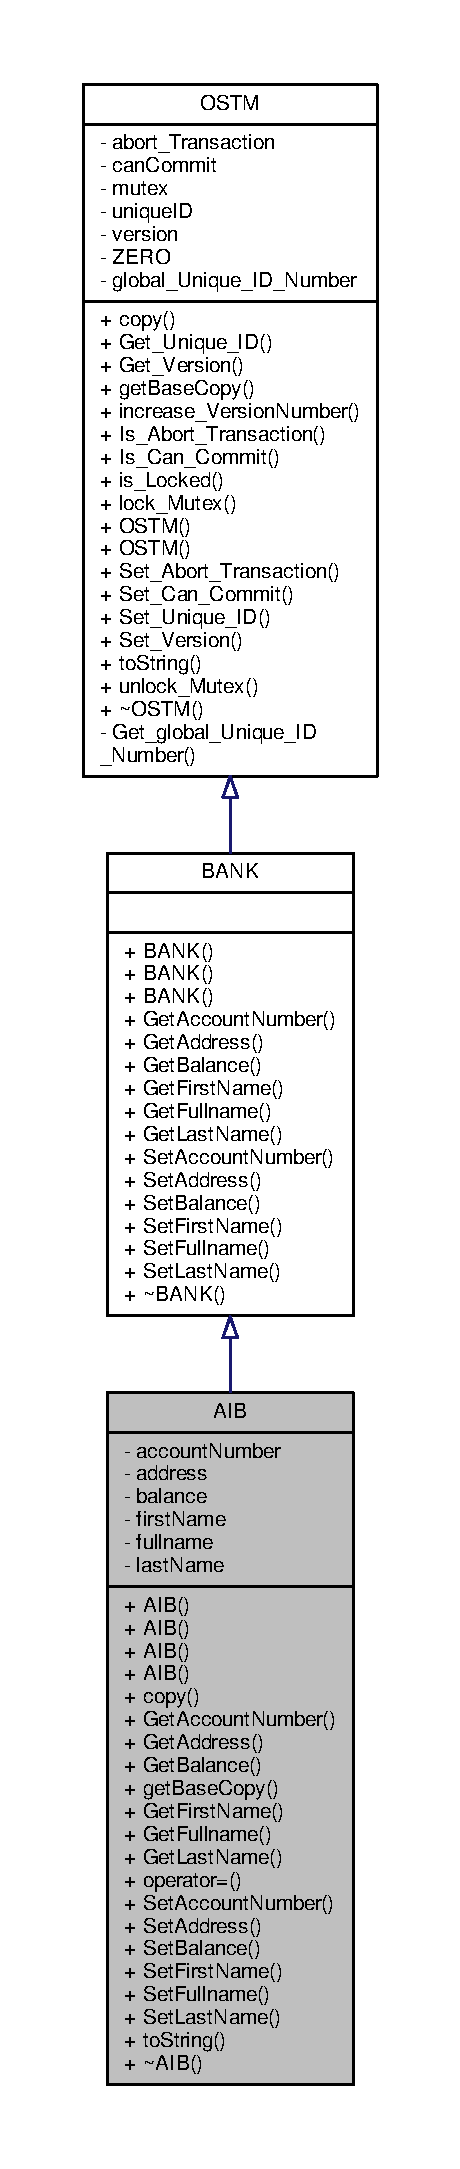
\includegraphics[height=550pt]{class_a_i_b__inherit__graph}
\end{center}
\end{figure}


Collaboration diagram for A\+IB\+:
\nopagebreak
\begin{figure}[H]
\begin{center}
\leavevmode
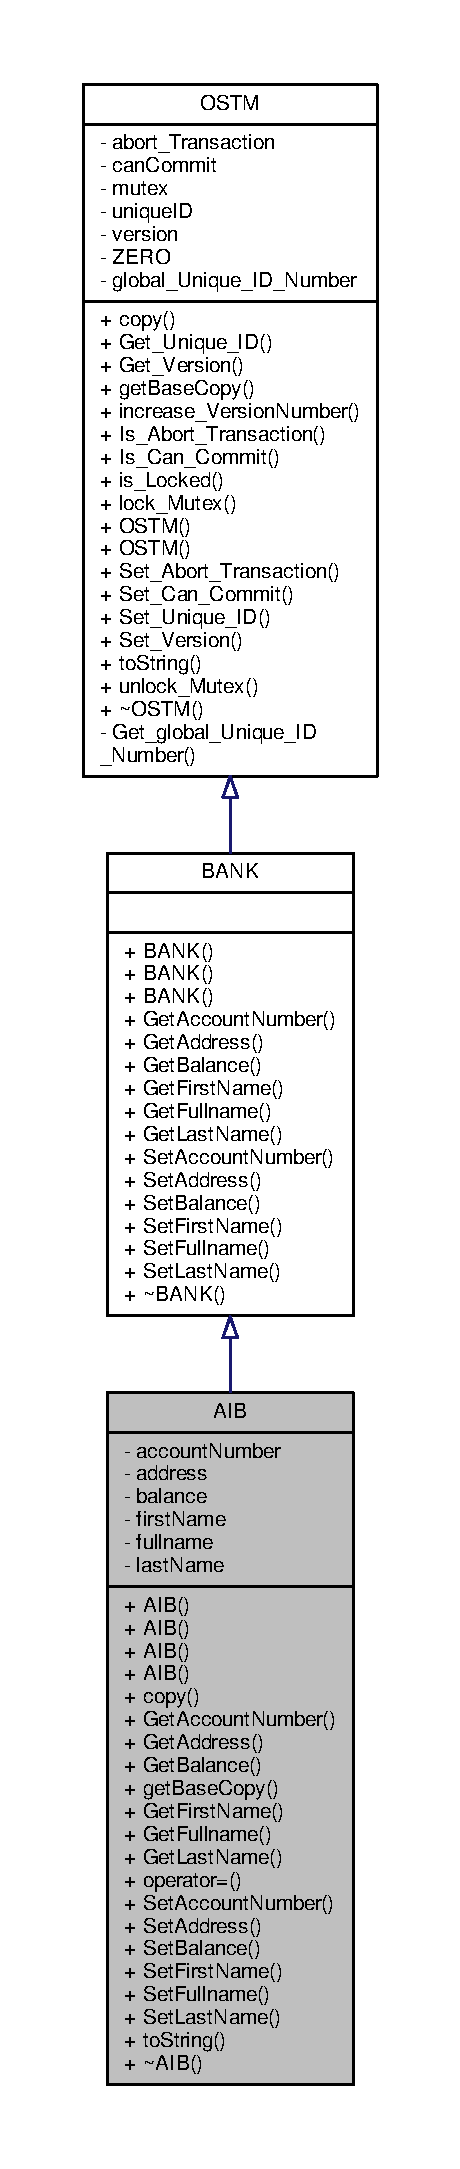
\includegraphics[height=550pt]{class_a_i_b__coll__graph}
\end{center}
\end{figure}
\subsubsection*{Public Member Functions}
\begin{DoxyCompactItemize}
\item 
\hyperlink{class_a_i_b_a4783110463bf12f937a85b62455faf38_a4783110463bf12f937a85b62455faf38}{A\+IB} ()
\item 
\hyperlink{class_a_i_b_a5fe3963becf294f6b1ce1a747f9122a0_a5fe3963becf294f6b1ce1a747f9122a0}{A\+IB} (int \hyperlink{class_a_i_b_aafc08efeec5b8c800c32ee32f20603a7_aafc08efeec5b8c800c32ee32f20603a7}{account\+Number}, double \hyperlink{class_a_i_b_a3c8d637bd997c1f062d844a88e2559ba_a3c8d637bd997c1f062d844a88e2559ba}{balance}, std\+::string \hyperlink{class_a_i_b_a869f72057cb63ebf0cfd257069e15c7c_a869f72057cb63ebf0cfd257069e15c7c}{first\+Name}, std\+::string \hyperlink{class_a_i_b_ace7b8b648d1b44b7ee2f4be002952b7a_ace7b8b648d1b44b7ee2f4be002952b7a}{last\+Name}, std\+::string \hyperlink{class_a_i_b_ae6a67cc33d1e5fa83a52a238e45ca3dc_ae6a67cc33d1e5fa83a52a238e45ca3dc}{address})
\item 
\hyperlink{class_a_i_b_aa0faccb7aadf423d12bddb2469ff5053_aa0faccb7aadf423d12bddb2469ff5053}{A\+IB} (std\+::shared\+\_\+ptr$<$ \hyperlink{class_b_a_n_k}{B\+A\+NK} $>$ obj, int \+\_\+version, int \+\_\+unique\+\_\+id)
\item 
\hyperlink{class_a_i_b_ab13d0db3498d59dbe6a946c469587c55_ab13d0db3498d59dbe6a946c469587c55}{A\+IB} (const \hyperlink{class_a_i_b}{A\+IB} \&orig)
\item 
virtual void \hyperlink{class_a_i_b_ad76f25ce86cb42028440f41c371903e0_ad76f25ce86cb42028440f41c371903e0}{copy} (std\+::shared\+\_\+ptr$<$ \hyperlink{class_o_s_t_m}{O\+S\+TM} $>$ to, std\+::shared\+\_\+ptr$<$ \hyperlink{class_o_s_t_m}{O\+S\+TM} $>$ from)
\begin{DoxyCompactList}\small\item\em copy function, make deep copy of the object/pointer \end{DoxyCompactList}\item 
virtual int \hyperlink{class_a_i_b_aef34bfbf20d767114e05b8b532cab777_aef34bfbf20d767114e05b8b532cab777}{Get\+Account\+Number} () const 
\begin{DoxyCompactList}\small\item\em Get\+Account\+Number getter for account\+Number private field. \end{DoxyCompactList}\item 
virtual std\+::string \hyperlink{class_a_i_b_a5092c8741fbe231531aa5aaa61d26b9c_a5092c8741fbe231531aa5aaa61d26b9c}{Get\+Address} () const 
\begin{DoxyCompactList}\small\item\em Get\+Address getter for address private field. \end{DoxyCompactList}\item 
virtual double \hyperlink{class_a_i_b_ac75087ae73c308bd946e47a71dc85b86_ac75087ae73c308bd946e47a71dc85b86}{Get\+Balance} () const 
\begin{DoxyCompactList}\small\item\em Get\+Balance getter for balance private field. \end{DoxyCompactList}\item 
virtual std\+::shared\+\_\+ptr$<$ \hyperlink{class_o_s_t_m}{O\+S\+TM} $>$ \hyperlink{class_a_i_b_a987107f3d7a04790f84c1e7eeee37575_a987107f3d7a04790f84c1e7eeee37575}{get\+Base\+Copy} (std\+::shared\+\_\+ptr$<$ \hyperlink{class_o_s_t_m}{O\+S\+TM} $>$ object)
\begin{DoxyCompactList}\small\item\em get\+Base\+Copy function, make deep copy of the object/pointer and Return a new std\+::shared\+\_\+ptr$<$\+B\+A\+N\+K$>$ type object \end{DoxyCompactList}\item 
virtual std\+::string \hyperlink{class_a_i_b_aa0833919c1c211481560cd88cb5b381b_aa0833919c1c211481560cd88cb5b381b}{Get\+First\+Name} () const 
\begin{DoxyCompactList}\small\item\em Get\+First\+Name getter for first\+Name private field. \end{DoxyCompactList}\item 
virtual std\+::string \hyperlink{class_a_i_b_a4fbad1d62d84d47e78b2b7065be14942_a4fbad1d62d84d47e78b2b7065be14942}{Get\+Fullname} () const 
\begin{DoxyCompactList}\small\item\em Get\+Fullname getter for fullname private field. \end{DoxyCompactList}\item 
virtual std\+::string \hyperlink{class_a_i_b_a1b09db7268734beeaf6a9e7e9d8feb02_a1b09db7268734beeaf6a9e7e9d8feb02}{Get\+Last\+Name} () const 
\begin{DoxyCompactList}\small\item\em Get\+Last\+Name getter for last\+Name private field. \end{DoxyCompactList}\item 
\hyperlink{class_a_i_b}{A\+IB} \hyperlink{class_a_i_b_a77b6f74ea3ef39cb1ccb916db7a48740_a77b6f74ea3ef39cb1ccb916db7a48740}{operator=} (const \hyperlink{class_a_i_b}{A\+IB} \&orig)
\item 
virtual void \hyperlink{class_a_i_b_ae582677d2d890f1728dedb9f43965df6_ae582677d2d890f1728dedb9f43965df6}{Set\+Account\+Number} (int \hyperlink{class_a_i_b_aafc08efeec5b8c800c32ee32f20603a7_aafc08efeec5b8c800c32ee32f20603a7}{account\+Number})
\begin{DoxyCompactList}\small\item\em Set\+Account\+Number setter for account\+Number private field. \end{DoxyCompactList}\item 
virtual void \hyperlink{class_a_i_b_ab5fd22fbbc0ea75a022aaeb7174fc450_ab5fd22fbbc0ea75a022aaeb7174fc450}{Set\+Address} (std\+::string \hyperlink{class_a_i_b_ae6a67cc33d1e5fa83a52a238e45ca3dc_ae6a67cc33d1e5fa83a52a238e45ca3dc}{address})
\begin{DoxyCompactList}\small\item\em Set\+Address setter for address private field. \end{DoxyCompactList}\item 
virtual void \hyperlink{class_a_i_b_ac286e13b8cf985bc88ce356b0eaada81_ac286e13b8cf985bc88ce356b0eaada81}{Set\+Balance} (double \hyperlink{class_a_i_b_a3c8d637bd997c1f062d844a88e2559ba_a3c8d637bd997c1f062d844a88e2559ba}{balance})
\begin{DoxyCompactList}\small\item\em Set\+Balance setter for balance private field. \end{DoxyCompactList}\item 
virtual void \hyperlink{class_a_i_b_a671e44bdbf1286d97d7a22295177dd2e_a671e44bdbf1286d97d7a22295177dd2e}{Set\+First\+Name} (std\+::string \hyperlink{class_a_i_b_a869f72057cb63ebf0cfd257069e15c7c_a869f72057cb63ebf0cfd257069e15c7c}{first\+Name})
\begin{DoxyCompactList}\small\item\em Set\+First\+Name setter for first\+Name private field. \end{DoxyCompactList}\item 
virtual void \hyperlink{class_a_i_b_a03def15426e627042951369ea18b97f6_a03def15426e627042951369ea18b97f6}{Set\+Fullname} (std\+::string \hyperlink{class_a_i_b_a818b0cc283af23127c067fb3fc751058_a818b0cc283af23127c067fb3fc751058}{fullname})
\begin{DoxyCompactList}\small\item\em Set\+Fullname setter for fullname private field. \end{DoxyCompactList}\item 
virtual void \hyperlink{class_a_i_b_afe4e3c7b481bf87437968dde2cc75882_afe4e3c7b481bf87437968dde2cc75882}{Set\+Last\+Name} (std\+::string \hyperlink{class_a_i_b_ace7b8b648d1b44b7ee2f4be002952b7a_ace7b8b648d1b44b7ee2f4be002952b7a}{last\+Name})
\begin{DoxyCompactList}\small\item\em Set\+Last\+Name setter for last\+Name private field. \end{DoxyCompactList}\item 
virtual void \hyperlink{class_a_i_b_aff0f0a0db75a17efec4bd500b888232d_aff0f0a0db75a17efec4bd500b888232d}{to\+String} ()
\begin{DoxyCompactList}\small\item\em to\+String function, displays the object values in formatted way \end{DoxyCompactList}\item 
virtual \hyperlink{class_a_i_b_a22b11c50b0986326c86315957528bf79_a22b11c50b0986326c86315957528bf79}{$\sim$\+A\+IB} ()
\end{DoxyCompactItemize}
\subsubsection*{Private Attributes}
\begin{DoxyCompactItemize}
\item 
int \hyperlink{class_a_i_b_aafc08efeec5b8c800c32ee32f20603a7_aafc08efeec5b8c800c32ee32f20603a7}{account\+Number}
\item 
std\+::string \hyperlink{class_a_i_b_ae6a67cc33d1e5fa83a52a238e45ca3dc_ae6a67cc33d1e5fa83a52a238e45ca3dc}{address}
\item 
double \hyperlink{class_a_i_b_a3c8d637bd997c1f062d844a88e2559ba_a3c8d637bd997c1f062d844a88e2559ba}{balance}
\item 
std\+::string \hyperlink{class_a_i_b_a869f72057cb63ebf0cfd257069e15c7c_a869f72057cb63ebf0cfd257069e15c7c}{first\+Name}
\item 
std\+::string \hyperlink{class_a_i_b_a818b0cc283af23127c067fb3fc751058_a818b0cc283af23127c067fb3fc751058}{fullname}
\item 
std\+::string \hyperlink{class_a_i_b_ace7b8b648d1b44b7ee2f4be002952b7a_ace7b8b648d1b44b7ee2f4be002952b7a}{last\+Name}
\end{DoxyCompactItemize}


\subsubsection{Detailed Description}
Class \hyperlink{class_a_i_b}{A\+IB} Inherit from \hyperlink{class_b_a_n_k}{B\+A\+NK} class 

Definition at line \hyperlink{_a_i_b_8h_source_l00023}{23} of file \hyperlink{_a_i_b_8h_source}{A\+I\+B.\+h}.



\subsubsection{Constructor \& Destructor Documentation}
\index{A\+IB@{A\+IB}!A\+IB@{A\+IB}}
\index{A\+IB@{A\+IB}!A\+IB@{A\+IB}}
\paragraph[{\texorpdfstring{A\+I\+B()}{AIB()}}]{\setlength{\rightskip}{0pt plus 5cm}A\+I\+B\+::\+A\+IB (
\begin{DoxyParamCaption}
{}
\end{DoxyParamCaption}
)\hspace{0.3cm}{\ttfamily [inline]}}\hypertarget{class_a_i_b_a4783110463bf12f937a85b62455faf38_a4783110463bf12f937a85b62455faf38}{}\label{class_a_i_b_a4783110463bf12f937a85b62455faf38_a4783110463bf12f937a85b62455faf38}
Constructor 

Definition at line \hyperlink{_a_i_b_8h_source_l00028}{28} of file \hyperlink{_a_i_b_8h_source}{A\+I\+B.\+h}.



References \hyperlink{_a_i_b_8h_source_l00123}{account\+Number}, \hyperlink{_a_i_b_8h_source_l00131}{address}, \hyperlink{_a_i_b_8h_source_l00127}{balance}, \hyperlink{_a_i_b_8h_source_l00115}{first\+Name}, \hyperlink{_a_i_b_8h_source_l00111}{fullname}, and \hyperlink{_a_i_b_8h_source_l00119}{last\+Name}.



Referenced by \hyperlink{_a_i_b_8h_source_l00061}{A\+I\+B()}, and \hyperlink{_a_i_b_8cpp_source_l00025}{get\+Base\+Copy()}.


\begin{DoxyCode}
00028          : \hyperlink{class_b_a_n_k_a0bc938356cebff14fb0560264abe5a34_a0bc938356cebff14fb0560264abe5a34}{BANK}()
00029     \{
00030         this->\hyperlink{class_a_i_b_aafc08efeec5b8c800c32ee32f20603a7_aafc08efeec5b8c800c32ee32f20603a7}{accountNumber} = 0;
00031         this->\hyperlink{class_a_i_b_a3c8d637bd997c1f062d844a88e2559ba_a3c8d637bd997c1f062d844a88e2559ba}{balance} = 50;
00032         this->\hyperlink{class_a_i_b_a869f72057cb63ebf0cfd257069e15c7c_a869f72057cb63ebf0cfd257069e15c7c}{firstName} = \textcolor{stringliteral}{"Joe"};
00033         this->\hyperlink{class_a_i_b_ace7b8b648d1b44b7ee2f4be002952b7a_ace7b8b648d1b44b7ee2f4be002952b7a}{lastName} = \textcolor{stringliteral}{"Blog"};
00034         this->\hyperlink{class_a_i_b_ae6a67cc33d1e5fa83a52a238e45ca3dc_ae6a67cc33d1e5fa83a52a238e45ca3dc}{address} = \textcolor{stringliteral}{"High street, Carlow"};
00035         this->\hyperlink{class_a_i_b_a818b0cc283af23127c067fb3fc751058_a818b0cc283af23127c067fb3fc751058}{fullname} = \hyperlink{class_a_i_b_a869f72057cb63ebf0cfd257069e15c7c_a869f72057cb63ebf0cfd257069e15c7c}{firstName} + \textcolor{stringliteral}{" "} + \hyperlink{class_a_i_b_ace7b8b648d1b44b7ee2f4be002952b7a_ace7b8b648d1b44b7ee2f4be002952b7a}{lastName};
00036     
00037     \};
\end{DoxyCode}


Here is the caller graph for this function\+:\nopagebreak
\begin{figure}[H]
\begin{center}
\leavevmode
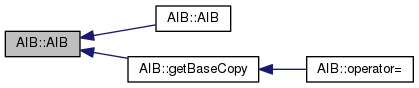
\includegraphics[width=350pt]{class_a_i_b_a4783110463bf12f937a85b62455faf38_a4783110463bf12f937a85b62455faf38_icgraph}
\end{center}
\end{figure}


\index{A\+IB@{A\+IB}!A\+IB@{A\+IB}}
\index{A\+IB@{A\+IB}!A\+IB@{A\+IB}}
\paragraph[{\texorpdfstring{A\+I\+B(int account\+Number, double balance, std\+::string first\+Name, std\+::string last\+Name, std\+::string address)}{AIB(int accountNumber, double balance, std::string firstName, std::string lastName, std::string address)}}]{\setlength{\rightskip}{0pt plus 5cm}A\+I\+B\+::\+A\+IB (
\begin{DoxyParamCaption}
\item[{int}]{account\+Number, }
\item[{double}]{balance, }
\item[{std\+::string}]{first\+Name, }
\item[{std\+::string}]{last\+Name, }
\item[{std\+::string}]{address}
\end{DoxyParamCaption}
)\hspace{0.3cm}{\ttfamily [inline]}}\hypertarget{class_a_i_b_a5fe3963becf294f6b1ce1a747f9122a0_a5fe3963becf294f6b1ce1a747f9122a0}{}\label{class_a_i_b_a5fe3963becf294f6b1ce1a747f9122a0_a5fe3963becf294f6b1ce1a747f9122a0}
Custom constructor 
\begin{DoxyParams}{Parameters}
{\em account\+Number} & integer \\
\hline
{\em balance} & double \\
\hline
{\em first\+Name} & string \\
\hline
{\em last\+Name} & string \\
\hline
{\em address} & string \\
\hline
\end{DoxyParams}


Definition at line \hyperlink{_a_i_b_8h_source_l00046}{46} of file \hyperlink{_a_i_b_8h_source}{A\+I\+B.\+h}.



References \hyperlink{_a_i_b_8h_source_l00123}{account\+Number}, \hyperlink{_a_i_b_8h_source_l00131}{address}, \hyperlink{_a_i_b_8h_source_l00127}{balance}, \hyperlink{_a_i_b_8h_source_l00115}{first\+Name}, \hyperlink{_a_i_b_8h_source_l00111}{fullname}, and \hyperlink{_a_i_b_8h_source_l00119}{last\+Name}.


\begin{DoxyCode}
00046                                                                                                       : 
      \hyperlink{class_b_a_n_k_a0bc938356cebff14fb0560264abe5a34_a0bc938356cebff14fb0560264abe5a34}{BANK}()
00047     \{
00048         this->\hyperlink{class_a_i_b_aafc08efeec5b8c800c32ee32f20603a7_aafc08efeec5b8c800c32ee32f20603a7}{accountNumber} = \hyperlink{class_a_i_b_aafc08efeec5b8c800c32ee32f20603a7_aafc08efeec5b8c800c32ee32f20603a7}{accountNumber};
00049         this->\hyperlink{class_a_i_b_a3c8d637bd997c1f062d844a88e2559ba_a3c8d637bd997c1f062d844a88e2559ba}{balance} = \hyperlink{class_a_i_b_a3c8d637bd997c1f062d844a88e2559ba_a3c8d637bd997c1f062d844a88e2559ba}{balance};
00050         this->\hyperlink{class_a_i_b_a869f72057cb63ebf0cfd257069e15c7c_a869f72057cb63ebf0cfd257069e15c7c}{firstName} = \hyperlink{class_a_i_b_a869f72057cb63ebf0cfd257069e15c7c_a869f72057cb63ebf0cfd257069e15c7c}{firstName};
00051         this->\hyperlink{class_a_i_b_ace7b8b648d1b44b7ee2f4be002952b7a_ace7b8b648d1b44b7ee2f4be002952b7a}{lastName} = \hyperlink{class_a_i_b_ace7b8b648d1b44b7ee2f4be002952b7a_ace7b8b648d1b44b7ee2f4be002952b7a}{lastName};
00052         this->\hyperlink{class_a_i_b_ae6a67cc33d1e5fa83a52a238e45ca3dc_ae6a67cc33d1e5fa83a52a238e45ca3dc}{address} = \hyperlink{class_a_i_b_ae6a67cc33d1e5fa83a52a238e45ca3dc_ae6a67cc33d1e5fa83a52a238e45ca3dc}{address};
00053         this->\hyperlink{class_a_i_b_a818b0cc283af23127c067fb3fc751058_a818b0cc283af23127c067fb3fc751058}{fullname} = \hyperlink{class_a_i_b_a869f72057cb63ebf0cfd257069e15c7c_a869f72057cb63ebf0cfd257069e15c7c}{firstName} + \textcolor{stringliteral}{" "} + \hyperlink{class_a_i_b_ace7b8b648d1b44b7ee2f4be002952b7a_ace7b8b648d1b44b7ee2f4be002952b7a}{lastName};
00054     \}; 
\end{DoxyCode}
\index{A\+IB@{A\+IB}!A\+IB@{A\+IB}}
\index{A\+IB@{A\+IB}!A\+IB@{A\+IB}}
\paragraph[{\texorpdfstring{A\+I\+B(std\+::shared\+\_\+ptr$<$ B\+A\+N\+K $>$ obj, int \+\_\+version, int \+\_\+unique\+\_\+id)}{AIB(std::shared_ptr< BANK > obj, int _version, int _unique_id)}}]{\setlength{\rightskip}{0pt plus 5cm}A\+I\+B\+::\+A\+IB (
\begin{DoxyParamCaption}
\item[{std\+::shared\+\_\+ptr$<$ {\bf B\+A\+NK} $>$}]{obj, }
\item[{int}]{\+\_\+version, }
\item[{int}]{\+\_\+unique\+\_\+id}
\end{DoxyParamCaption}
)\hspace{0.3cm}{\ttfamily [inline]}}\hypertarget{class_a_i_b_aa0faccb7aadf423d12bddb2469ff5053_aa0faccb7aadf423d12bddb2469ff5053}{}\label{class_a_i_b_aa0faccb7aadf423d12bddb2469ff5053_aa0faccb7aadf423d12bddb2469ff5053}
Custom constructor, used by the library for deep copying 
\begin{DoxyParams}{Parameters}
{\em obj} & std\+::shared\+\_\+ptr$<$\+B\+A\+N\+K$>$ \\
\hline
{\em \+\_\+version} & integer \\
\hline
{\em \+\_\+unique\+\_\+id} & integer \\
\hline
\end{DoxyParams}


Definition at line \hyperlink{_a_i_b_8h_source_l00061}{61} of file \hyperlink{_a_i_b_8h_source}{A\+I\+B.\+h}.



References \hyperlink{_a_i_b_8h_source_l00123}{account\+Number}, \hyperlink{_a_i_b_8h_source_l00131}{address}, \hyperlink{_a_i_b_8h_source_l00028}{A\+I\+B()}, \hyperlink{_a_i_b_8h_source_l00127}{balance}, \hyperlink{_a_i_b_8h_source_l00115}{first\+Name}, \hyperlink{_a_i_b_8h_source_l00111}{fullname}, and \hyperlink{_a_i_b_8h_source_l00119}{last\+Name}.


\begin{DoxyCode}
00061                                                               : \hyperlink{class_b_a_n_k_a0bc938356cebff14fb0560264abe5a34_a0bc938356cebff14fb0560264abe5a34}{BANK}(\_version, \_unique\_id)
00062     \{
00063         this->\hyperlink{class_a_i_b_aafc08efeec5b8c800c32ee32f20603a7_aafc08efeec5b8c800c32ee32f20603a7}{accountNumber} = obj->GetAccountNumber();
00064         this->\hyperlink{class_a_i_b_a3c8d637bd997c1f062d844a88e2559ba_a3c8d637bd997c1f062d844a88e2559ba}{balance} = obj->GetBalance();
00065         this->\hyperlink{class_a_i_b_a869f72057cb63ebf0cfd257069e15c7c_a869f72057cb63ebf0cfd257069e15c7c}{firstName} = obj->GetFirstName();
00066         this->\hyperlink{class_a_i_b_ace7b8b648d1b44b7ee2f4be002952b7a_ace7b8b648d1b44b7ee2f4be002952b7a}{lastName} = obj->GetLastName();
00067         this->\hyperlink{class_a_i_b_ae6a67cc33d1e5fa83a52a238e45ca3dc_ae6a67cc33d1e5fa83a52a238e45ca3dc}{address} = obj->GetAddress();
00068         this->\hyperlink{class_a_i_b_a818b0cc283af23127c067fb3fc751058_a818b0cc283af23127c067fb3fc751058}{fullname} = obj->GetFirstName() + \textcolor{stringliteral}{" "} + obj->GetLastName(); 
00069         
00070     \};
\end{DoxyCode}


Here is the call graph for this function\+:\nopagebreak
\begin{figure}[H]
\begin{center}
\leavevmode
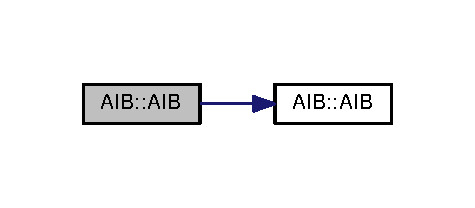
\includegraphics[width=228pt]{class_a_i_b_aa0faccb7aadf423d12bddb2469ff5053_aa0faccb7aadf423d12bddb2469ff5053_cgraph}
\end{center}
\end{figure}


\index{A\+IB@{A\+IB}!A\+IB@{A\+IB}}
\index{A\+IB@{A\+IB}!A\+IB@{A\+IB}}
\paragraph[{\texorpdfstring{A\+I\+B(const A\+I\+B \&orig)}{AIB(const AIB &orig)}}]{\setlength{\rightskip}{0pt plus 5cm}A\+I\+B\+::\+A\+IB (
\begin{DoxyParamCaption}
\item[{const {\bf A\+IB} \&}]{orig}
\end{DoxyParamCaption}
)}\hypertarget{class_a_i_b_ab13d0db3498d59dbe6a946c469587c55_ab13d0db3498d59dbe6a946c469587c55}{}\label{class_a_i_b_ab13d0db3498d59dbe6a946c469587c55_ab13d0db3498d59dbe6a946c469587c55}
Copy constructor \index{A\+IB@{A\+IB}!````~A\+IB@{$\sim$\+A\+IB}}
\index{````~A\+IB@{$\sim$\+A\+IB}!A\+IB@{A\+IB}}
\paragraph[{\texorpdfstring{$\sim$\+A\+I\+B()}{~AIB()}}]{\setlength{\rightskip}{0pt plus 5cm}A\+I\+B\+::$\sim$\+A\+IB (
\begin{DoxyParamCaption}
{}
\end{DoxyParamCaption}
)\hspace{0.3cm}{\ttfamily [virtual]}}\hypertarget{class_a_i_b_a22b11c50b0986326c86315957528bf79_a22b11c50b0986326c86315957528bf79}{}\label{class_a_i_b_a22b11c50b0986326c86315957528bf79_a22b11c50b0986326c86315957528bf79}
de-\/constructor 

Definition at line \hyperlink{_a_i_b_8cpp_source_l00019}{19} of file \hyperlink{_a_i_b_8cpp_source}{A\+I\+B.\+cpp}.



Referenced by \hyperlink{_a_i_b_8h_source_l00078}{operator=()}.


\begin{DoxyCode}
00019           \{
00020 \}
\end{DoxyCode}


Here is the caller graph for this function\+:\nopagebreak
\begin{figure}[H]
\begin{center}
\leavevmode
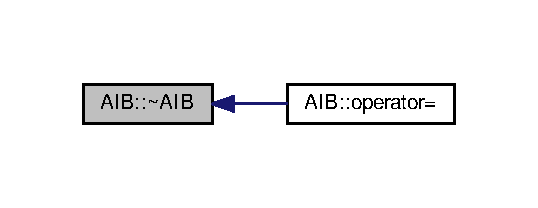
\includegraphics[width=258pt]{class_a_i_b_a22b11c50b0986326c86315957528bf79_a22b11c50b0986326c86315957528bf79_icgraph}
\end{center}
\end{figure}




\subsubsection{Member Function Documentation}
\index{A\+IB@{A\+IB}!copy@{copy}}
\index{copy@{copy}!A\+IB@{A\+IB}}
\paragraph[{\texorpdfstring{copy(std\+::shared\+\_\+ptr$<$ O\+S\+T\+M $>$ to, std\+::shared\+\_\+ptr$<$ O\+S\+T\+M $>$ from)}{copy(std::shared_ptr< OSTM > to, std::shared_ptr< OSTM > from)}}]{\setlength{\rightskip}{0pt plus 5cm}void A\+I\+B\+::copy (
\begin{DoxyParamCaption}
\item[{std\+::shared\+\_\+ptr$<$ {\bf O\+S\+TM} $>$}]{to, }
\item[{std\+::shared\+\_\+ptr$<$ {\bf O\+S\+TM} $>$}]{from}
\end{DoxyParamCaption}
)\hspace{0.3cm}{\ttfamily [virtual]}}\hypertarget{class_a_i_b_ad76f25ce86cb42028440f41c371903e0_ad76f25ce86cb42028440f41c371903e0}{}\label{class_a_i_b_ad76f25ce86cb42028440f41c371903e0_ad76f25ce86cb42028440f41c371903e0}


copy function, make deep copy of the object/pointer 

Implement \hyperlink{class_o_s_t_m}{O\+S\+TM} virtual methods in cpp class


\begin{DoxyParams}{Parameters}
{\em to} & std\+::shared\+\_\+ptr$<$\+O\+S\+T\+M$>$, \hyperlink{class_b_a_n_k}{B\+A\+NK} type shared pointer used to copy into the values \\
\hline
{\em from} & std\+::shared\+\_\+ptr$<$\+O\+S\+T\+M$>$, \hyperlink{class_b_a_n_k}{B\+A\+NK} type shared ponter used to get object values tfrom copy \\
\hline
\end{DoxyParams}
Dynamic cast from \hyperlink{class_o_s_t_m}{O\+S\+TM} to \hyperlink{class_a_i_b}{A\+IB}

Dynamic cast from \hyperlink{class_o_s_t_m}{O\+S\+TM} to \hyperlink{class_a_i_b}{A\+IB}

Set values fro object to object

Set values fro object to object

Set values fro object to object

Set values fro object to object 

Reimplemented from \hyperlink{class_o_s_t_m_a535d90fced5adbb70312c92f3778e08d_a535d90fced5adbb70312c92f3778e08d}{O\+S\+TM}.



Definition at line \hyperlink{_a_i_b_8cpp_source_l00041}{41} of file \hyperlink{_a_i_b_8cpp_source}{A\+I\+B.\+cpp}.



References \hyperlink{_o_s_t_m_8cpp_source_l00075}{O\+S\+T\+M\+::\+Set\+\_\+\+Unique\+\_\+\+I\+D()}.



Referenced by \hyperlink{_a_i_b_8h_source_l00078}{operator=()}.


\begin{DoxyCode}
00041                                                               \{
00042 
00044     std::shared\_ptr<AIB> objTO = std::dynamic\_pointer\_cast<\hyperlink{class_a_i_b}{AIB}>(to);
00046     std::shared\_ptr<AIB> objFROM = std::dynamic\_pointer\_cast<\hyperlink{class_a_i_b}{AIB}>(from);
00048     objTO->\hyperlink{class_o_s_t_m_ab5019a32185631c08abbf826422f2d93_ab5019a32185631c08abbf826422f2d93}{Set\_Unique\_ID}(objFROM->Get\_Unique\_ID());
00050     objTO->Set\_Version(objFROM->Get\_Version());
00052     objTO->SetAccountNumber(objFROM->GetAccountNumber());
00054     objTO->SetBalance(objFROM->GetBalance());
00055 \}
\end{DoxyCode}


Here is the call graph for this function\+:\nopagebreak
\begin{figure}[H]
\begin{center}
\leavevmode
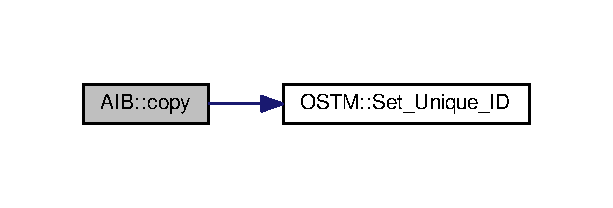
\includegraphics[width=294pt]{class_a_i_b_ad76f25ce86cb42028440f41c371903e0_ad76f25ce86cb42028440f41c371903e0_cgraph}
\end{center}
\end{figure}




Here is the caller graph for this function\+:\nopagebreak
\begin{figure}[H]
\begin{center}
\leavevmode
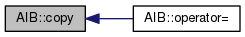
\includegraphics[width=256pt]{class_a_i_b_ad76f25ce86cb42028440f41c371903e0_ad76f25ce86cb42028440f41c371903e0_icgraph}
\end{center}
\end{figure}


\index{A\+IB@{A\+IB}!Get\+Account\+Number@{Get\+Account\+Number}}
\index{Get\+Account\+Number@{Get\+Account\+Number}!A\+IB@{A\+IB}}
\paragraph[{\texorpdfstring{Get\+Account\+Number() const }{GetAccountNumber() const }}]{\setlength{\rightskip}{0pt plus 5cm}int A\+I\+B\+::\+Get\+Account\+Number (
\begin{DoxyParamCaption}
{}
\end{DoxyParamCaption}
) const\hspace{0.3cm}{\ttfamily [virtual]}}\hypertarget{class_a_i_b_aef34bfbf20d767114e05b8b532cab777_aef34bfbf20d767114e05b8b532cab777}{}\label{class_a_i_b_aef34bfbf20d767114e05b8b532cab777_aef34bfbf20d767114e05b8b532cab777}


Get\+Account\+Number getter for account\+Number private field. 



Reimplemented from \hyperlink{class_b_a_n_k_a62adf3cea60d863a4a10eeee485fa1aa_a62adf3cea60d863a4a10eeee485fa1aa}{B\+A\+NK}.



Definition at line \hyperlink{_a_i_b_8cpp_source_l00096}{96} of file \hyperlink{_a_i_b_8cpp_source}{A\+I\+B.\+cpp}.



References \hyperlink{_a_i_b_8h_source_l00123}{account\+Number}.



Referenced by \hyperlink{_a_i_b_8h_source_l00078}{operator=()}, and \hyperlink{_a_i_b_8cpp_source_l00059}{to\+String()}.


\begin{DoxyCode}
00096                                 \{
00097     \textcolor{keywordflow}{return} \hyperlink{class_a_i_b_aafc08efeec5b8c800c32ee32f20603a7_aafc08efeec5b8c800c32ee32f20603a7}{accountNumber};
00098 \}
\end{DoxyCode}


Here is the caller graph for this function\+:\nopagebreak
\begin{figure}[H]
\begin{center}
\leavevmode
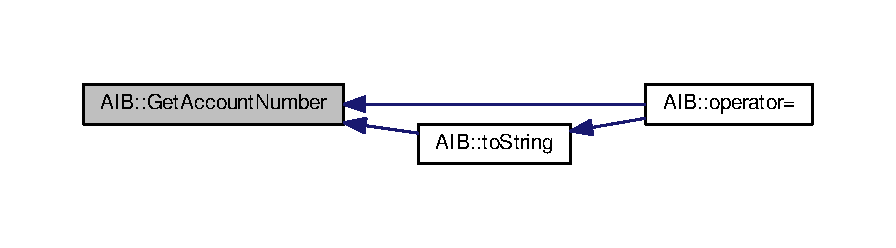
\includegraphics[width=350pt]{class_a_i_b_aef34bfbf20d767114e05b8b532cab777_aef34bfbf20d767114e05b8b532cab777_icgraph}
\end{center}
\end{figure}


\index{A\+IB@{A\+IB}!Get\+Address@{Get\+Address}}
\index{Get\+Address@{Get\+Address}!A\+IB@{A\+IB}}
\paragraph[{\texorpdfstring{Get\+Address() const }{GetAddress() const }}]{\setlength{\rightskip}{0pt plus 5cm}std\+::string A\+I\+B\+::\+Get\+Address (
\begin{DoxyParamCaption}
{}
\end{DoxyParamCaption}
) const\hspace{0.3cm}{\ttfamily [virtual]}}\hypertarget{class_a_i_b_a5092c8741fbe231531aa5aaa61d26b9c_a5092c8741fbe231531aa5aaa61d26b9c}{}\label{class_a_i_b_a5092c8741fbe231531aa5aaa61d26b9c_a5092c8741fbe231531aa5aaa61d26b9c}


Get\+Address getter for address private field. 



Reimplemented from \hyperlink{class_b_a_n_k_a358741f647f9494026e02fd3fd27cde6_a358741f647f9494026e02fd3fd27cde6}{B\+A\+NK}.



Definition at line \hyperlink{_a_i_b_8cpp_source_l00072}{72} of file \hyperlink{_a_i_b_8cpp_source}{A\+I\+B.\+cpp}.



References \hyperlink{_a_i_b_8h_source_l00131}{address}.



Referenced by \hyperlink{_a_i_b_8h_source_l00078}{operator=()}.


\begin{DoxyCode}
00072                                 \{
00073     \textcolor{keywordflow}{return} \hyperlink{class_a_i_b_ae6a67cc33d1e5fa83a52a238e45ca3dc_ae6a67cc33d1e5fa83a52a238e45ca3dc}{address};
00074 \}
\end{DoxyCode}


Here is the caller graph for this function\+:\nopagebreak
\begin{figure}[H]
\begin{center}
\leavevmode
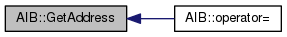
\includegraphics[width=287pt]{class_a_i_b_a5092c8741fbe231531aa5aaa61d26b9c_a5092c8741fbe231531aa5aaa61d26b9c_icgraph}
\end{center}
\end{figure}


\index{A\+IB@{A\+IB}!Get\+Balance@{Get\+Balance}}
\index{Get\+Balance@{Get\+Balance}!A\+IB@{A\+IB}}
\paragraph[{\texorpdfstring{Get\+Balance() const }{GetBalance() const }}]{\setlength{\rightskip}{0pt plus 5cm}double A\+I\+B\+::\+Get\+Balance (
\begin{DoxyParamCaption}
{}
\end{DoxyParamCaption}
) const\hspace{0.3cm}{\ttfamily [virtual]}}\hypertarget{class_a_i_b_ac75087ae73c308bd946e47a71dc85b86_ac75087ae73c308bd946e47a71dc85b86}{}\label{class_a_i_b_ac75087ae73c308bd946e47a71dc85b86_ac75087ae73c308bd946e47a71dc85b86}


Get\+Balance getter for balance private field. 



Reimplemented from \hyperlink{class_b_a_n_k_a7ac46c74859cebdc933cb27e148d18b1_a7ac46c74859cebdc933cb27e148d18b1}{B\+A\+NK}.



Definition at line \hyperlink{_a_i_b_8cpp_source_l00084}{84} of file \hyperlink{_a_i_b_8cpp_source}{A\+I\+B.\+cpp}.



References \hyperlink{_a_i_b_8h_source_l00127}{balance}.



Referenced by \hyperlink{_a_i_b_8h_source_l00078}{operator=()}, and \hyperlink{_a_i_b_8cpp_source_l00059}{to\+String()}.


\begin{DoxyCode}
00084                              \{
00085     \textcolor{keywordflow}{return} \hyperlink{class_a_i_b_a3c8d637bd997c1f062d844a88e2559ba_a3c8d637bd997c1f062d844a88e2559ba}{balance};
00086 \}
\end{DoxyCode}


Here is the caller graph for this function\+:\nopagebreak
\begin{figure}[H]
\begin{center}
\leavevmode
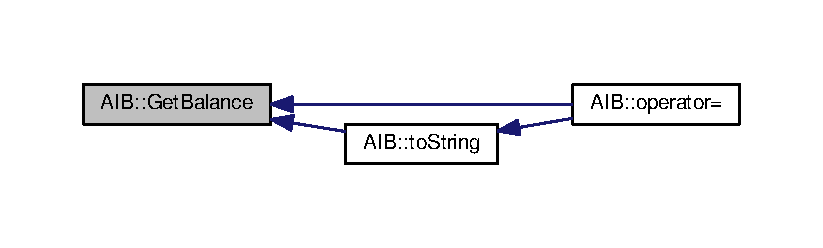
\includegraphics[width=350pt]{class_a_i_b_ac75087ae73c308bd946e47a71dc85b86_ac75087ae73c308bd946e47a71dc85b86_icgraph}
\end{center}
\end{figure}


\index{A\+IB@{A\+IB}!get\+Base\+Copy@{get\+Base\+Copy}}
\index{get\+Base\+Copy@{get\+Base\+Copy}!A\+IB@{A\+IB}}
\paragraph[{\texorpdfstring{get\+Base\+Copy(std\+::shared\+\_\+ptr$<$ O\+S\+T\+M $>$ object)}{getBaseCopy(std::shared_ptr< OSTM > object)}}]{\setlength{\rightskip}{0pt plus 5cm}std\+::shared\+\_\+ptr$<$ {\bf O\+S\+TM} $>$ A\+I\+B\+::get\+Base\+Copy (
\begin{DoxyParamCaption}
\item[{std\+::shared\+\_\+ptr$<$ {\bf O\+S\+TM} $>$}]{object}
\end{DoxyParamCaption}
)\hspace{0.3cm}{\ttfamily [virtual]}}\hypertarget{class_a_i_b_a987107f3d7a04790f84c1e7eeee37575_a987107f3d7a04790f84c1e7eeee37575}{}\label{class_a_i_b_a987107f3d7a04790f84c1e7eeee37575_a987107f3d7a04790f84c1e7eeee37575}


get\+Base\+Copy function, make deep copy of the object/pointer and Return a new std\+::shared\+\_\+ptr$<$\+B\+A\+N\+K$>$ type object 


\begin{DoxyParams}{Parameters}
{\em object} & is a \hyperlink{class_o_s_t_m}{O\+S\+TM} type shared pointer use to create a new copy of the pointer \\
\hline
\end{DoxyParams}
Dynamic cast from \hyperlink{class_o_s_t_m}{O\+S\+TM} to \hyperlink{class_b_a_n_k}{B\+A\+NK} type

\hyperlink{class_b_a_n_k}{B\+A\+NK} type Instance creation shared pointer

Dynamic cast from \hyperlink{class_b_a_n_k}{B\+A\+NK} to \hyperlink{class_o_s_t_m}{O\+S\+TM} type

Return new \hyperlink{class_o_s_t_m}{O\+S\+TM} copy onject 

Reimplemented from \hyperlink{class_o_s_t_m_a0bfa3763bd441407dd6365f42714f94c_a0bfa3763bd441407dd6365f42714f94c}{O\+S\+TM}.



Definition at line \hyperlink{_a_i_b_8cpp_source_l00025}{25} of file \hyperlink{_a_i_b_8cpp_source}{A\+I\+B.\+cpp}.



References \hyperlink{_a_i_b_8h_source_l00028}{A\+I\+B()}.



Referenced by \hyperlink{_a_i_b_8h_source_l00078}{operator=()}.


\begin{DoxyCode}
00026 \{
00028     std::shared\_ptr<BANK> objTO = std::dynamic\_pointer\_cast<\hyperlink{class_b_a_n_k}{BANK}>(object);
00030     std::shared\_ptr<BANK> obj(\textcolor{keyword}{new} \hyperlink{class_a_i_b_a4783110463bf12f937a85b62455faf38_a4783110463bf12f937a85b62455faf38}{AIB}(objTO, object->Get\_Version(),\textcolor{keywordtype}{object}->Get\_Unique\_ID()));
00032     std::shared\_ptr<OSTM> ostm\_obj = std::dynamic\_pointer\_cast<\hyperlink{class_o_s_t_m}{OSTM}>(obj);
00034     \textcolor{keywordflow}{return} ostm\_obj;
00035 \}
\end{DoxyCode}


Here is the call graph for this function\+:\nopagebreak
\begin{figure}[H]
\begin{center}
\leavevmode
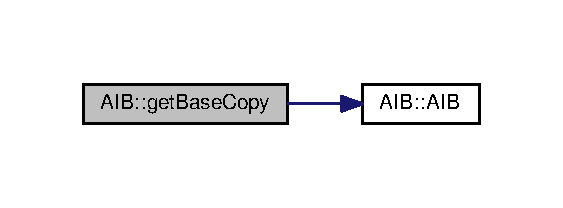
\includegraphics[width=270pt]{class_a_i_b_a987107f3d7a04790f84c1e7eeee37575_a987107f3d7a04790f84c1e7eeee37575_cgraph}
\end{center}
\end{figure}




Here is the caller graph for this function\+:\nopagebreak
\begin{figure}[H]
\begin{center}
\leavevmode
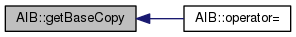
\includegraphics[width=294pt]{class_a_i_b_a987107f3d7a04790f84c1e7eeee37575_a987107f3d7a04790f84c1e7eeee37575_icgraph}
\end{center}
\end{figure}


\index{A\+IB@{A\+IB}!Get\+First\+Name@{Get\+First\+Name}}
\index{Get\+First\+Name@{Get\+First\+Name}!A\+IB@{A\+IB}}
\paragraph[{\texorpdfstring{Get\+First\+Name() const }{GetFirstName() const }}]{\setlength{\rightskip}{0pt plus 5cm}std\+::string A\+I\+B\+::\+Get\+First\+Name (
\begin{DoxyParamCaption}
{}
\end{DoxyParamCaption}
) const\hspace{0.3cm}{\ttfamily [virtual]}}\hypertarget{class_a_i_b_aa0833919c1c211481560cd88cb5b381b_aa0833919c1c211481560cd88cb5b381b}{}\label{class_a_i_b_aa0833919c1c211481560cd88cb5b381b_aa0833919c1c211481560cd88cb5b381b}


Get\+First\+Name getter for first\+Name private field. 



Reimplemented from \hyperlink{class_b_a_n_k_ad0ba1c785c67e7d4760dc8776f3d4bca_ad0ba1c785c67e7d4760dc8776f3d4bca}{B\+A\+NK}.



Definition at line \hyperlink{_a_i_b_8cpp_source_l00120}{120} of file \hyperlink{_a_i_b_8cpp_source}{A\+I\+B.\+cpp}.



References \hyperlink{_a_i_b_8h_source_l00115}{first\+Name}.



Referenced by \hyperlink{_a_i_b_8h_source_l00078}{operator=()}, and \hyperlink{_a_i_b_8cpp_source_l00059}{to\+String()}.


\begin{DoxyCode}
00120                                   \{
00121     \textcolor{keywordflow}{return} \hyperlink{class_a_i_b_a869f72057cb63ebf0cfd257069e15c7c_a869f72057cb63ebf0cfd257069e15c7c}{firstName};
00122 \}
\end{DoxyCode}


Here is the caller graph for this function\+:\nopagebreak
\begin{figure}[H]
\begin{center}
\leavevmode
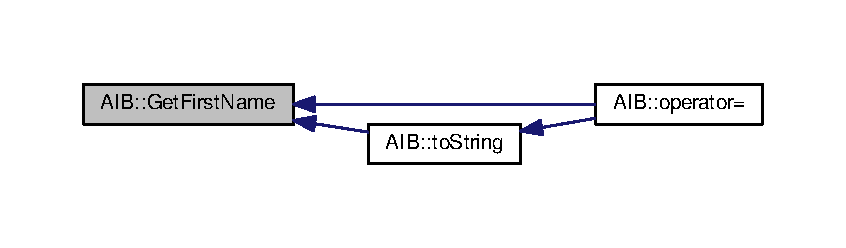
\includegraphics[width=350pt]{class_a_i_b_aa0833919c1c211481560cd88cb5b381b_aa0833919c1c211481560cd88cb5b381b_icgraph}
\end{center}
\end{figure}


\index{A\+IB@{A\+IB}!Get\+Fullname@{Get\+Fullname}}
\index{Get\+Fullname@{Get\+Fullname}!A\+IB@{A\+IB}}
\paragraph[{\texorpdfstring{Get\+Fullname() const }{GetFullname() const }}]{\setlength{\rightskip}{0pt plus 5cm}std\+::string A\+I\+B\+::\+Get\+Fullname (
\begin{DoxyParamCaption}
{}
\end{DoxyParamCaption}
) const\hspace{0.3cm}{\ttfamily [virtual]}}\hypertarget{class_a_i_b_a4fbad1d62d84d47e78b2b7065be14942_a4fbad1d62d84d47e78b2b7065be14942}{}\label{class_a_i_b_a4fbad1d62d84d47e78b2b7065be14942_a4fbad1d62d84d47e78b2b7065be14942}


Get\+Fullname getter for fullname private field. 



Reimplemented from \hyperlink{class_b_a_n_k_aa1528c533bf6389bc8d7f3eeca114bab_aa1528c533bf6389bc8d7f3eeca114bab}{B\+A\+NK}.



Definition at line \hyperlink{_a_i_b_8cpp_source_l00132}{132} of file \hyperlink{_a_i_b_8cpp_source}{A\+I\+B.\+cpp}.



References \hyperlink{_a_i_b_8h_source_l00111}{fullname}.



Referenced by \hyperlink{_a_i_b_8h_source_l00078}{operator=()}.


\begin{DoxyCode}
00132                                  \{
00133     \textcolor{keywordflow}{return} \hyperlink{class_a_i_b_a818b0cc283af23127c067fb3fc751058_a818b0cc283af23127c067fb3fc751058}{fullname};
00134 \}
\end{DoxyCode}


Here is the caller graph for this function\+:\nopagebreak
\begin{figure}[H]
\begin{center}
\leavevmode
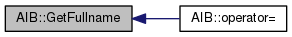
\includegraphics[width=291pt]{class_a_i_b_a4fbad1d62d84d47e78b2b7065be14942_a4fbad1d62d84d47e78b2b7065be14942_icgraph}
\end{center}
\end{figure}


\index{A\+IB@{A\+IB}!Get\+Last\+Name@{Get\+Last\+Name}}
\index{Get\+Last\+Name@{Get\+Last\+Name}!A\+IB@{A\+IB}}
\paragraph[{\texorpdfstring{Get\+Last\+Name() const }{GetLastName() const }}]{\setlength{\rightskip}{0pt plus 5cm}std\+::string A\+I\+B\+::\+Get\+Last\+Name (
\begin{DoxyParamCaption}
{}
\end{DoxyParamCaption}
) const\hspace{0.3cm}{\ttfamily [virtual]}}\hypertarget{class_a_i_b_a1b09db7268734beeaf6a9e7e9d8feb02_a1b09db7268734beeaf6a9e7e9d8feb02}{}\label{class_a_i_b_a1b09db7268734beeaf6a9e7e9d8feb02_a1b09db7268734beeaf6a9e7e9d8feb02}


Get\+Last\+Name getter for last\+Name private field. 



Reimplemented from \hyperlink{class_b_a_n_k_a4612063ec2bfd6d883a77a0d3697af90_a4612063ec2bfd6d883a77a0d3697af90}{B\+A\+NK}.



Definition at line \hyperlink{_a_i_b_8cpp_source_l00108}{108} of file \hyperlink{_a_i_b_8cpp_source}{A\+I\+B.\+cpp}.



References \hyperlink{_a_i_b_8h_source_l00119}{last\+Name}.



Referenced by \hyperlink{_a_i_b_8h_source_l00078}{operator=()}, and \hyperlink{_a_i_b_8cpp_source_l00059}{to\+String()}.


\begin{DoxyCode}
00108                                  \{
00109     \textcolor{keywordflow}{return} \hyperlink{class_a_i_b_ace7b8b648d1b44b7ee2f4be002952b7a_ace7b8b648d1b44b7ee2f4be002952b7a}{lastName};
00110 \}
\end{DoxyCode}


Here is the caller graph for this function\+:\nopagebreak
\begin{figure}[H]
\begin{center}
\leavevmode
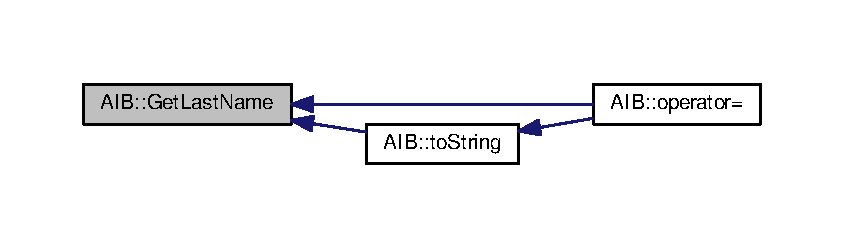
\includegraphics[width=350pt]{class_a_i_b_a1b09db7268734beeaf6a9e7e9d8feb02_a1b09db7268734beeaf6a9e7e9d8feb02_icgraph}
\end{center}
\end{figure}


\index{A\+IB@{A\+IB}!operator=@{operator=}}
\index{operator=@{operator=}!A\+IB@{A\+IB}}
\paragraph[{\texorpdfstring{operator=(const A\+I\+B \&orig)}{operator=(const AIB &orig)}}]{\setlength{\rightskip}{0pt plus 5cm}{\bf A\+IB} A\+I\+B\+::operator= (
\begin{DoxyParamCaption}
\item[{const {\bf A\+IB} \&}]{orig}
\end{DoxyParamCaption}
)\hspace{0.3cm}{\ttfamily [inline]}}\hypertarget{class_a_i_b_a77b6f74ea3ef39cb1ccb916db7a48740_a77b6f74ea3ef39cb1ccb916db7a48740}{}\label{class_a_i_b_a77b6f74ea3ef39cb1ccb916db7a48740_a77b6f74ea3ef39cb1ccb916db7a48740}
Operator function 

Definition at line \hyperlink{_a_i_b_8h_source_l00078}{78} of file \hyperlink{_a_i_b_8h_source}{A\+I\+B.\+h}.



References \hyperlink{_a_i_b_8h_source_l00123}{account\+Number}, \hyperlink{_a_i_b_8h_source_l00131}{address}, \hyperlink{_a_i_b_8h_source_l00127}{balance}, \hyperlink{_a_i_b_8cpp_source_l00041}{copy()}, \hyperlink{_a_i_b_8h_source_l00115}{first\+Name}, \hyperlink{_a_i_b_8h_source_l00111}{fullname}, \hyperlink{_a_i_b_8cpp_source_l00096}{Get\+Account\+Number()}, \hyperlink{_a_i_b_8cpp_source_l00072}{Get\+Address()}, \hyperlink{_a_i_b_8cpp_source_l00084}{Get\+Balance()}, \hyperlink{_a_i_b_8cpp_source_l00025}{get\+Base\+Copy()}, \hyperlink{_a_i_b_8cpp_source_l00120}{Get\+First\+Name()}, \hyperlink{_a_i_b_8cpp_source_l00132}{Get\+Fullname()}, \hyperlink{_a_i_b_8cpp_source_l00108}{Get\+Last\+Name()}, \hyperlink{_a_i_b_8h_source_l00119}{last\+Name}, \hyperlink{_a_i_b_8cpp_source_l00090}{Set\+Account\+Number()}, \hyperlink{_a_i_b_8cpp_source_l00066}{Set\+Address()}, \hyperlink{_a_i_b_8cpp_source_l00078}{Set\+Balance()}, \hyperlink{_a_i_b_8cpp_source_l00114}{Set\+First\+Name()}, \hyperlink{_a_i_b_8cpp_source_l00126}{Set\+Fullname()}, \hyperlink{_a_i_b_8cpp_source_l00102}{Set\+Last\+Name()}, \hyperlink{_a_i_b_8cpp_source_l00059}{to\+String()}, and \hyperlink{_a_i_b_8cpp_source_l00019}{$\sim$\+A\+I\+B()}.


\begin{DoxyCode}
00078 \{\};
\end{DoxyCode}


Here is the call graph for this function\+:\nopagebreak
\begin{figure}[H]
\begin{center}
\leavevmode
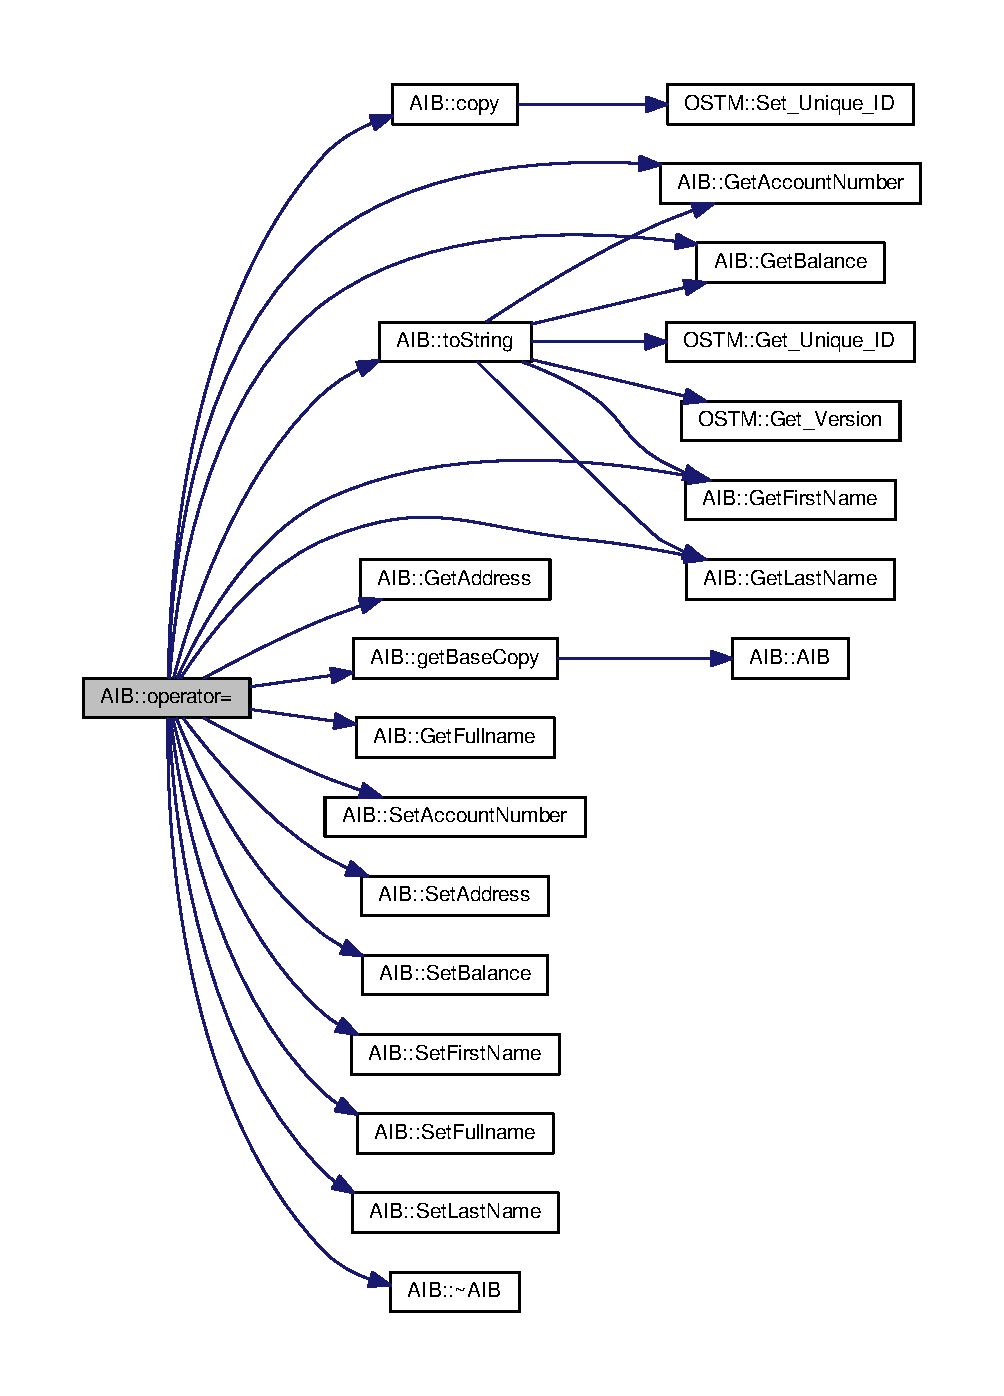
\includegraphics[width=350pt]{class_a_i_b_a77b6f74ea3ef39cb1ccb916db7a48740_a77b6f74ea3ef39cb1ccb916db7a48740_cgraph}
\end{center}
\end{figure}


\index{A\+IB@{A\+IB}!Set\+Account\+Number@{Set\+Account\+Number}}
\index{Set\+Account\+Number@{Set\+Account\+Number}!A\+IB@{A\+IB}}
\paragraph[{\texorpdfstring{Set\+Account\+Number(int account\+Number)}{SetAccountNumber(int accountNumber)}}]{\setlength{\rightskip}{0pt plus 5cm}void A\+I\+B\+::\+Set\+Account\+Number (
\begin{DoxyParamCaption}
\item[{int}]{account\+Number}
\end{DoxyParamCaption}
)\hspace{0.3cm}{\ttfamily [virtual]}}\hypertarget{class_a_i_b_ae582677d2d890f1728dedb9f43965df6_ae582677d2d890f1728dedb9f43965df6}{}\label{class_a_i_b_ae582677d2d890f1728dedb9f43965df6_ae582677d2d890f1728dedb9f43965df6}


Set\+Account\+Number setter for account\+Number private field. 



Reimplemented from \hyperlink{class_b_a_n_k_a9d8fb8bde35d63eca7e9f87d22b45752_a9d8fb8bde35d63eca7e9f87d22b45752}{B\+A\+NK}.



Definition at line \hyperlink{_a_i_b_8cpp_source_l00090}{90} of file \hyperlink{_a_i_b_8cpp_source}{A\+I\+B.\+cpp}.



References \hyperlink{_a_i_b_8h_source_l00123}{account\+Number}.



Referenced by \hyperlink{_a_i_b_8h_source_l00078}{operator=()}.


\begin{DoxyCode}
00090                                             \{
00091     this->\hyperlink{class_a_i_b_aafc08efeec5b8c800c32ee32f20603a7_aafc08efeec5b8c800c32ee32f20603a7}{accountNumber} = \hyperlink{class_a_i_b_aafc08efeec5b8c800c32ee32f20603a7_aafc08efeec5b8c800c32ee32f20603a7}{accountNumber};
00092 \}
\end{DoxyCode}


Here is the caller graph for this function\+:\nopagebreak
\begin{figure}[H]
\begin{center}
\leavevmode
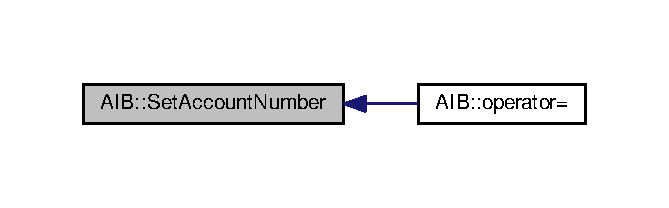
\includegraphics[width=321pt]{class_a_i_b_ae582677d2d890f1728dedb9f43965df6_ae582677d2d890f1728dedb9f43965df6_icgraph}
\end{center}
\end{figure}


\index{A\+IB@{A\+IB}!Set\+Address@{Set\+Address}}
\index{Set\+Address@{Set\+Address}!A\+IB@{A\+IB}}
\paragraph[{\texorpdfstring{Set\+Address(std\+::string address)}{SetAddress(std::string address)}}]{\setlength{\rightskip}{0pt plus 5cm}void A\+I\+B\+::\+Set\+Address (
\begin{DoxyParamCaption}
\item[{std\+::string}]{address}
\end{DoxyParamCaption}
)\hspace{0.3cm}{\ttfamily [virtual]}}\hypertarget{class_a_i_b_ab5fd22fbbc0ea75a022aaeb7174fc450_ab5fd22fbbc0ea75a022aaeb7174fc450}{}\label{class_a_i_b_ab5fd22fbbc0ea75a022aaeb7174fc450_ab5fd22fbbc0ea75a022aaeb7174fc450}


Set\+Address setter for address private field. 



Reimplemented from \hyperlink{class_b_a_n_k_a52ad99454b2059d44967868157208393_a52ad99454b2059d44967868157208393}{B\+A\+NK}.



Definition at line \hyperlink{_a_i_b_8cpp_source_l00066}{66} of file \hyperlink{_a_i_b_8cpp_source}{A\+I\+B.\+cpp}.



References \hyperlink{_a_i_b_8h_source_l00131}{address}.



Referenced by \hyperlink{_a_i_b_8h_source_l00078}{operator=()}.


\begin{DoxyCode}
00066                                       \{
00067     this->\hyperlink{class_a_i_b_ae6a67cc33d1e5fa83a52a238e45ca3dc_ae6a67cc33d1e5fa83a52a238e45ca3dc}{address} = \hyperlink{class_a_i_b_ae6a67cc33d1e5fa83a52a238e45ca3dc_ae6a67cc33d1e5fa83a52a238e45ca3dc}{address};
00068 \}
\end{DoxyCode}


Here is the caller graph for this function\+:\nopagebreak
\begin{figure}[H]
\begin{center}
\leavevmode
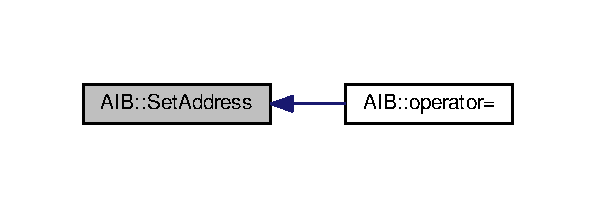
\includegraphics[width=286pt]{class_a_i_b_ab5fd22fbbc0ea75a022aaeb7174fc450_ab5fd22fbbc0ea75a022aaeb7174fc450_icgraph}
\end{center}
\end{figure}


\index{A\+IB@{A\+IB}!Set\+Balance@{Set\+Balance}}
\index{Set\+Balance@{Set\+Balance}!A\+IB@{A\+IB}}
\paragraph[{\texorpdfstring{Set\+Balance(double balance)}{SetBalance(double balance)}}]{\setlength{\rightskip}{0pt plus 5cm}void A\+I\+B\+::\+Set\+Balance (
\begin{DoxyParamCaption}
\item[{double}]{balance}
\end{DoxyParamCaption}
)\hspace{0.3cm}{\ttfamily [virtual]}}\hypertarget{class_a_i_b_ac286e13b8cf985bc88ce356b0eaada81_ac286e13b8cf985bc88ce356b0eaada81}{}\label{class_a_i_b_ac286e13b8cf985bc88ce356b0eaada81_ac286e13b8cf985bc88ce356b0eaada81}


Set\+Balance setter for balance private field. 



Reimplemented from \hyperlink{class_b_a_n_k_ae3e45b407bf8ec7175662442ea24b7c0_ae3e45b407bf8ec7175662442ea24b7c0}{B\+A\+NK}.



Definition at line \hyperlink{_a_i_b_8cpp_source_l00078}{78} of file \hyperlink{_a_i_b_8cpp_source}{A\+I\+B.\+cpp}.



References \hyperlink{_a_i_b_8h_source_l00127}{balance}.



Referenced by \hyperlink{_a_i_b_8h_source_l00078}{operator=()}.


\begin{DoxyCode}
00078                                    \{
00079     this->\hyperlink{class_a_i_b_a3c8d637bd997c1f062d844a88e2559ba_a3c8d637bd997c1f062d844a88e2559ba}{balance} = \hyperlink{class_a_i_b_a3c8d637bd997c1f062d844a88e2559ba_a3c8d637bd997c1f062d844a88e2559ba}{balance};
00080 \}
\end{DoxyCode}


Here is the caller graph for this function\+:\nopagebreak
\begin{figure}[H]
\begin{center}
\leavevmode
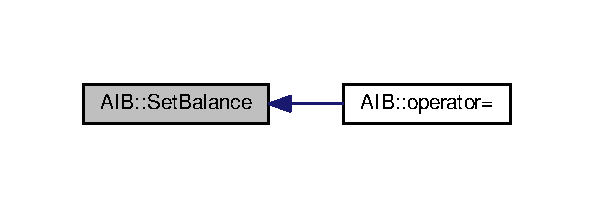
\includegraphics[width=285pt]{class_a_i_b_ac286e13b8cf985bc88ce356b0eaada81_ac286e13b8cf985bc88ce356b0eaada81_icgraph}
\end{center}
\end{figure}


\index{A\+IB@{A\+IB}!Set\+First\+Name@{Set\+First\+Name}}
\index{Set\+First\+Name@{Set\+First\+Name}!A\+IB@{A\+IB}}
\paragraph[{\texorpdfstring{Set\+First\+Name(std\+::string first\+Name)}{SetFirstName(std::string firstName)}}]{\setlength{\rightskip}{0pt plus 5cm}void A\+I\+B\+::\+Set\+First\+Name (
\begin{DoxyParamCaption}
\item[{std\+::string}]{first\+Name}
\end{DoxyParamCaption}
)\hspace{0.3cm}{\ttfamily [virtual]}}\hypertarget{class_a_i_b_a671e44bdbf1286d97d7a22295177dd2e_a671e44bdbf1286d97d7a22295177dd2e}{}\label{class_a_i_b_a671e44bdbf1286d97d7a22295177dd2e_a671e44bdbf1286d97d7a22295177dd2e}


Set\+First\+Name setter for first\+Name private field. 



Reimplemented from \hyperlink{class_b_a_n_k_a547cb9f21be894f045bb3cec6b12525c_a547cb9f21be894f045bb3cec6b12525c}{B\+A\+NK}.



Definition at line \hyperlink{_a_i_b_8cpp_source_l00114}{114} of file \hyperlink{_a_i_b_8cpp_source}{A\+I\+B.\+cpp}.



References \hyperlink{_a_i_b_8h_source_l00115}{first\+Name}.



Referenced by \hyperlink{_a_i_b_8h_source_l00078}{operator=()}.


\begin{DoxyCode}
00114                                           \{
00115     this->\hyperlink{class_a_i_b_a869f72057cb63ebf0cfd257069e15c7c_a869f72057cb63ebf0cfd257069e15c7c}{firstName} = \hyperlink{class_a_i_b_a869f72057cb63ebf0cfd257069e15c7c_a869f72057cb63ebf0cfd257069e15c7c}{firstName};
00116 \}
\end{DoxyCode}


Here is the caller graph for this function\+:\nopagebreak
\begin{figure}[H]
\begin{center}
\leavevmode
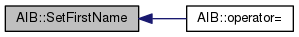
\includegraphics[width=296pt]{class_a_i_b_a671e44bdbf1286d97d7a22295177dd2e_a671e44bdbf1286d97d7a22295177dd2e_icgraph}
\end{center}
\end{figure}


\index{A\+IB@{A\+IB}!Set\+Fullname@{Set\+Fullname}}
\index{Set\+Fullname@{Set\+Fullname}!A\+IB@{A\+IB}}
\paragraph[{\texorpdfstring{Set\+Fullname(std\+::string fullname)}{SetFullname(std::string fullname)}}]{\setlength{\rightskip}{0pt plus 5cm}void A\+I\+B\+::\+Set\+Fullname (
\begin{DoxyParamCaption}
\item[{std\+::string}]{fullname}
\end{DoxyParamCaption}
)\hspace{0.3cm}{\ttfamily [virtual]}}\hypertarget{class_a_i_b_a03def15426e627042951369ea18b97f6_a03def15426e627042951369ea18b97f6}{}\label{class_a_i_b_a03def15426e627042951369ea18b97f6_a03def15426e627042951369ea18b97f6}


Set\+Fullname setter for fullname private field. 



Reimplemented from \hyperlink{class_b_a_n_k_a8845dbfc7ddfbc2e0c0efda561a70ec3_a8845dbfc7ddfbc2e0c0efda561a70ec3}{B\+A\+NK}.



Definition at line \hyperlink{_a_i_b_8cpp_source_l00126}{126} of file \hyperlink{_a_i_b_8cpp_source}{A\+I\+B.\+cpp}.



References \hyperlink{_a_i_b_8h_source_l00111}{fullname}.



Referenced by \hyperlink{_a_i_b_8h_source_l00078}{operator=()}.


\begin{DoxyCode}
00126                                         \{
00127     this->\hyperlink{class_a_i_b_a818b0cc283af23127c067fb3fc751058_a818b0cc283af23127c067fb3fc751058}{fullname} = \hyperlink{class_a_i_b_a818b0cc283af23127c067fb3fc751058_a818b0cc283af23127c067fb3fc751058}{fullname};
00128 \}
\end{DoxyCode}


Here is the caller graph for this function\+:\nopagebreak
\begin{figure}[H]
\begin{center}
\leavevmode
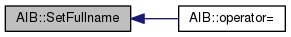
\includegraphics[width=290pt]{class_a_i_b_a03def15426e627042951369ea18b97f6_a03def15426e627042951369ea18b97f6_icgraph}
\end{center}
\end{figure}


\index{A\+IB@{A\+IB}!Set\+Last\+Name@{Set\+Last\+Name}}
\index{Set\+Last\+Name@{Set\+Last\+Name}!A\+IB@{A\+IB}}
\paragraph[{\texorpdfstring{Set\+Last\+Name(std\+::string last\+Name)}{SetLastName(std::string lastName)}}]{\setlength{\rightskip}{0pt plus 5cm}void A\+I\+B\+::\+Set\+Last\+Name (
\begin{DoxyParamCaption}
\item[{std\+::string}]{last\+Name}
\end{DoxyParamCaption}
)\hspace{0.3cm}{\ttfamily [virtual]}}\hypertarget{class_a_i_b_afe4e3c7b481bf87437968dde2cc75882_afe4e3c7b481bf87437968dde2cc75882}{}\label{class_a_i_b_afe4e3c7b481bf87437968dde2cc75882_afe4e3c7b481bf87437968dde2cc75882}


Set\+Last\+Name setter for last\+Name private field. 



Reimplemented from \hyperlink{class_b_a_n_k_a2dc1b7664f9e3b005cb33e71b2ba42ee_a2dc1b7664f9e3b005cb33e71b2ba42ee}{B\+A\+NK}.



Definition at line \hyperlink{_a_i_b_8cpp_source_l00102}{102} of file \hyperlink{_a_i_b_8cpp_source}{A\+I\+B.\+cpp}.



References \hyperlink{_a_i_b_8h_source_l00119}{last\+Name}.



Referenced by \hyperlink{_a_i_b_8h_source_l00078}{operator=()}.


\begin{DoxyCode}
00102                                         \{
00103     this->\hyperlink{class_a_i_b_ace7b8b648d1b44b7ee2f4be002952b7a_ace7b8b648d1b44b7ee2f4be002952b7a}{lastName} = \hyperlink{class_a_i_b_ace7b8b648d1b44b7ee2f4be002952b7a_ace7b8b648d1b44b7ee2f4be002952b7a}{lastName};
00104 \}
\end{DoxyCode}


Here is the caller graph for this function\+:\nopagebreak
\begin{figure}[H]
\begin{center}
\leavevmode
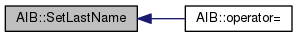
\includegraphics[width=295pt]{class_a_i_b_afe4e3c7b481bf87437968dde2cc75882_afe4e3c7b481bf87437968dde2cc75882_icgraph}
\end{center}
\end{figure}


\index{A\+IB@{A\+IB}!to\+String@{to\+String}}
\index{to\+String@{to\+String}!A\+IB@{A\+IB}}
\paragraph[{\texorpdfstring{to\+String()}{toString()}}]{\setlength{\rightskip}{0pt plus 5cm}void A\+I\+B\+::to\+String (
\begin{DoxyParamCaption}
{}
\end{DoxyParamCaption}
)\hspace{0.3cm}{\ttfamily [virtual]}}\hypertarget{class_a_i_b_aff0f0a0db75a17efec4bd500b888232d_aff0f0a0db75a17efec4bd500b888232d}{}\label{class_a_i_b_aff0f0a0db75a17efec4bd500b888232d_aff0f0a0db75a17efec4bd500b888232d}


to\+String function, displays the object values in formatted way 



Reimplemented from \hyperlink{class_o_s_t_m_a513396a115f2987fd07c203309ae8a59_a513396a115f2987fd07c203309ae8a59}{O\+S\+TM}.



Definition at line \hyperlink{_a_i_b_8cpp_source_l00059}{59} of file \hyperlink{_a_i_b_8cpp_source}{A\+I\+B.\+cpp}.



References \hyperlink{_o_s_t_m_8cpp_source_l00082}{O\+S\+T\+M\+::\+Get\+\_\+\+Unique\+\_\+\+I\+D()}, \hyperlink{_o_s_t_m_8cpp_source_l00100}{O\+S\+T\+M\+::\+Get\+\_\+\+Version()}, \hyperlink{_a_i_b_8cpp_source_l00096}{Get\+Account\+Number()}, \hyperlink{_a_i_b_8cpp_source_l00084}{Get\+Balance()}, \hyperlink{_a_i_b_8cpp_source_l00120}{Get\+First\+Name()}, and \hyperlink{_a_i_b_8cpp_source_l00108}{Get\+Last\+Name()}.



Referenced by \hyperlink{_a_i_b_8h_source_l00078}{operator=()}.


\begin{DoxyCode}
00060 \{
00061     std::cout << \textcolor{stringliteral}{"\(\backslash\)nAIB BANK"} << \textcolor{stringliteral}{"\(\backslash\)nUnique ID : "} << this->\hyperlink{class_o_s_t_m_a5a01a8b98d16b1d1904ecf9356e7b71d_a5a01a8b98d16b1d1904ecf9356e7b71d}{Get\_Unique\_ID}() << \textcolor{stringliteral}{"\(\backslash\)nInt account :
       "} << this->\hyperlink{class_a_i_b_aef34bfbf20d767114e05b8b532cab777_aef34bfbf20d767114e05b8b532cab777}{GetAccountNumber}() << \textcolor{stringliteral}{"\(\backslash\)nDouble value : "} << this->
      \hyperlink{class_a_i_b_ac75087ae73c308bd946e47a71dc85b86_ac75087ae73c308bd946e47a71dc85b86}{GetBalance}() << \textcolor{stringliteral}{"\(\backslash\)nFirst name: "} << this->\hyperlink{class_a_i_b_aa0833919c1c211481560cd88cb5b381b_aa0833919c1c211481560cd88cb5b381b}{GetFirstName}() << \textcolor{stringliteral}{"\(\backslash\)nLast name : "} << 
      this->\hyperlink{class_a_i_b_a1b09db7268734beeaf6a9e7e9d8feb02_a1b09db7268734beeaf6a9e7e9d8feb02}{GetLastName}()  << \textcolor{stringliteral}{"\(\backslash\)nVersion number : "} << this->\hyperlink{class_o_s_t_m_a1f1db9d482f22c8e7caa17dfb340626b_a1f1db9d482f22c8e7caa17dfb340626b}{Get\_Version}() << std::endl;
00062 \}
\end{DoxyCode}


Here is the call graph for this function\+:\nopagebreak
\begin{figure}[H]
\begin{center}
\leavevmode
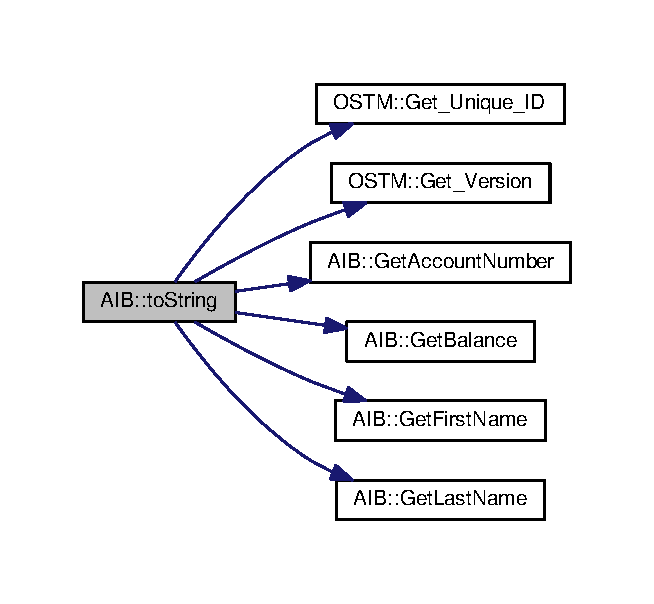
\includegraphics[width=314pt]{class_a_i_b_aff0f0a0db75a17efec4bd500b888232d_aff0f0a0db75a17efec4bd500b888232d_cgraph}
\end{center}
\end{figure}




Here is the caller graph for this function\+:\nopagebreak
\begin{figure}[H]
\begin{center}
\leavevmode
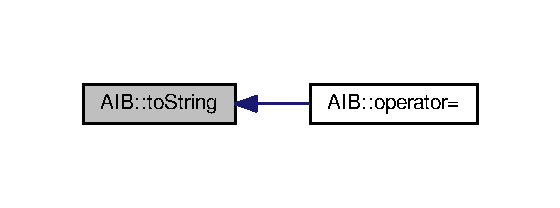
\includegraphics[width=269pt]{class_a_i_b_aff0f0a0db75a17efec4bd500b888232d_aff0f0a0db75a17efec4bd500b888232d_icgraph}
\end{center}
\end{figure}




\subsubsection{Member Data Documentation}
\index{A\+IB@{A\+IB}!account\+Number@{account\+Number}}
\index{account\+Number@{account\+Number}!A\+IB@{A\+IB}}
\paragraph[{\texorpdfstring{account\+Number}{accountNumber}}]{\setlength{\rightskip}{0pt plus 5cm}int A\+I\+B\+::account\+Number\hspace{0.3cm}{\ttfamily [private]}}\hypertarget{class_a_i_b_aafc08efeec5b8c800c32ee32f20603a7_aafc08efeec5b8c800c32ee32f20603a7}{}\label{class_a_i_b_aafc08efeec5b8c800c32ee32f20603a7_aafc08efeec5b8c800c32ee32f20603a7}
account\+Number int object private filed 

Definition at line \hyperlink{_a_i_b_8h_source_l00123}{123} of file \hyperlink{_a_i_b_8h_source}{A\+I\+B.\+h}.



Referenced by \hyperlink{_a_i_b_8h_source_l00028}{A\+I\+B()}, \hyperlink{_a_i_b_8cpp_source_l00096}{Get\+Account\+Number()}, \hyperlink{_a_i_b_8h_source_l00078}{operator=()}, and \hyperlink{_a_i_b_8cpp_source_l00090}{Set\+Account\+Number()}.

\index{A\+IB@{A\+IB}!address@{address}}
\index{address@{address}!A\+IB@{A\+IB}}
\paragraph[{\texorpdfstring{address}{address}}]{\setlength{\rightskip}{0pt plus 5cm}std\+::string A\+I\+B\+::address\hspace{0.3cm}{\ttfamily [private]}}\hypertarget{class_a_i_b_ae6a67cc33d1e5fa83a52a238e45ca3dc_ae6a67cc33d1e5fa83a52a238e45ca3dc}{}\label{class_a_i_b_ae6a67cc33d1e5fa83a52a238e45ca3dc_ae6a67cc33d1e5fa83a52a238e45ca3dc}
address string object private filed 

Definition at line \hyperlink{_a_i_b_8h_source_l00131}{131} of file \hyperlink{_a_i_b_8h_source}{A\+I\+B.\+h}.



Referenced by \hyperlink{_a_i_b_8h_source_l00028}{A\+I\+B()}, \hyperlink{_a_i_b_8cpp_source_l00072}{Get\+Address()}, \hyperlink{_a_i_b_8h_source_l00078}{operator=()}, and \hyperlink{_a_i_b_8cpp_source_l00066}{Set\+Address()}.

\index{A\+IB@{A\+IB}!balance@{balance}}
\index{balance@{balance}!A\+IB@{A\+IB}}
\paragraph[{\texorpdfstring{balance}{balance}}]{\setlength{\rightskip}{0pt plus 5cm}double A\+I\+B\+::balance\hspace{0.3cm}{\ttfamily [private]}}\hypertarget{class_a_i_b_a3c8d637bd997c1f062d844a88e2559ba_a3c8d637bd997c1f062d844a88e2559ba}{}\label{class_a_i_b_a3c8d637bd997c1f062d844a88e2559ba_a3c8d637bd997c1f062d844a88e2559ba}
balance double object private filed 

Definition at line \hyperlink{_a_i_b_8h_source_l00127}{127} of file \hyperlink{_a_i_b_8h_source}{A\+I\+B.\+h}.



Referenced by \hyperlink{_a_i_b_8h_source_l00028}{A\+I\+B()}, \hyperlink{_a_i_b_8cpp_source_l00084}{Get\+Balance()}, \hyperlink{_a_i_b_8h_source_l00078}{operator=()}, and \hyperlink{_a_i_b_8cpp_source_l00078}{Set\+Balance()}.

\index{A\+IB@{A\+IB}!first\+Name@{first\+Name}}
\index{first\+Name@{first\+Name}!A\+IB@{A\+IB}}
\paragraph[{\texorpdfstring{first\+Name}{firstName}}]{\setlength{\rightskip}{0pt plus 5cm}std\+::string A\+I\+B\+::first\+Name\hspace{0.3cm}{\ttfamily [private]}}\hypertarget{class_a_i_b_a869f72057cb63ebf0cfd257069e15c7c_a869f72057cb63ebf0cfd257069e15c7c}{}\label{class_a_i_b_a869f72057cb63ebf0cfd257069e15c7c_a869f72057cb63ebf0cfd257069e15c7c}
first\+Name string object private filed 

Definition at line \hyperlink{_a_i_b_8h_source_l00115}{115} of file \hyperlink{_a_i_b_8h_source}{A\+I\+B.\+h}.



Referenced by \hyperlink{_a_i_b_8h_source_l00028}{A\+I\+B()}, \hyperlink{_a_i_b_8cpp_source_l00120}{Get\+First\+Name()}, \hyperlink{_a_i_b_8h_source_l00078}{operator=()}, and \hyperlink{_a_i_b_8cpp_source_l00114}{Set\+First\+Name()}.

\index{A\+IB@{A\+IB}!fullname@{fullname}}
\index{fullname@{fullname}!A\+IB@{A\+IB}}
\paragraph[{\texorpdfstring{fullname}{fullname}}]{\setlength{\rightskip}{0pt plus 5cm}std\+::string A\+I\+B\+::fullname\hspace{0.3cm}{\ttfamily [private]}}\hypertarget{class_a_i_b_a818b0cc283af23127c067fb3fc751058_a818b0cc283af23127c067fb3fc751058}{}\label{class_a_i_b_a818b0cc283af23127c067fb3fc751058_a818b0cc283af23127c067fb3fc751058}
fullname string object private filed 

Definition at line \hyperlink{_a_i_b_8h_source_l00111}{111} of file \hyperlink{_a_i_b_8h_source}{A\+I\+B.\+h}.



Referenced by \hyperlink{_a_i_b_8h_source_l00028}{A\+I\+B()}, \hyperlink{_a_i_b_8cpp_source_l00132}{Get\+Fullname()}, \hyperlink{_a_i_b_8h_source_l00078}{operator=()}, and \hyperlink{_a_i_b_8cpp_source_l00126}{Set\+Fullname()}.

\index{A\+IB@{A\+IB}!last\+Name@{last\+Name}}
\index{last\+Name@{last\+Name}!A\+IB@{A\+IB}}
\paragraph[{\texorpdfstring{last\+Name}{lastName}}]{\setlength{\rightskip}{0pt plus 5cm}std\+::string A\+I\+B\+::last\+Name\hspace{0.3cm}{\ttfamily [private]}}\hypertarget{class_a_i_b_ace7b8b648d1b44b7ee2f4be002952b7a_ace7b8b648d1b44b7ee2f4be002952b7a}{}\label{class_a_i_b_ace7b8b648d1b44b7ee2f4be002952b7a_ace7b8b648d1b44b7ee2f4be002952b7a}
last\+Name string object private filed 

Definition at line \hyperlink{_a_i_b_8h_source_l00119}{119} of file \hyperlink{_a_i_b_8h_source}{A\+I\+B.\+h}.



Referenced by \hyperlink{_a_i_b_8h_source_l00028}{A\+I\+B()}, \hyperlink{_a_i_b_8cpp_source_l00108}{Get\+Last\+Name()}, \hyperlink{_a_i_b_8h_source_l00078}{operator=()}, and \hyperlink{_a_i_b_8cpp_source_l00102}{Set\+Last\+Name()}.



The documentation for this class was generated from the following files\+:\begin{DoxyCompactItemize}
\item 
\hyperlink{_a_i_b_8h}{A\+I\+B.\+h}\item 
\hyperlink{_a_i_b_8cpp}{A\+I\+B.\+cpp}\end{DoxyCompactItemize}

\section{B\+A\+NK Class Reference}
\label{class_b_a_n_k}\index{B\+A\+NK@{B\+A\+NK}}


{\ttfamily \#include $<$B\+A\+N\+K.\+h$>$}

Inheritance diagram for B\+A\+NK\+:\begin{figure}[H]
\begin{center}
\leavevmode
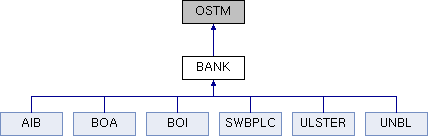
\includegraphics[height=3.000000cm]{class_b_a_n_k}
\end{center}
\end{figure}
\subsection*{Public Member Functions}
\begin{DoxyCompactItemize}
\item 
{\bf B\+A\+NK} ()
\item 
{\bf B\+A\+NK} (int \+\_\+version, int \+\_\+unique\+\_\+id)
\item 
{\bf B\+A\+NK} (const {\bf B\+A\+NK} \&orig)
\item 
virtual {\bf $\sim$\+B\+A\+NK} ()
\item 
virtual void {\bfseries Set\+Address} (std\+::string address)\label{class_b_a_n_k_a52ad99454b2059d44967868157208393}

\item 
virtual std\+::string {\bfseries Get\+Address} () const \label{class_b_a_n_k_a358741f647f9494026e02fd3fd27cde6}

\item 
virtual void {\bfseries Set\+Balance} (double balance)\label{class_b_a_n_k_ae3e45b407bf8ec7175662442ea24b7c0}

\item 
virtual double {\bfseries Get\+Balance} () const \label{class_b_a_n_k_a7ac46c74859cebdc933cb27e148d18b1}

\item 
virtual void {\bfseries Set\+Account\+Number} (int account\+Number)\label{class_b_a_n_k_a9d8fb8bde35d63eca7e9f87d22b45752}

\item 
virtual int {\bfseries Get\+Account\+Number} () const \label{class_b_a_n_k_a62adf3cea60d863a4a10eeee485fa1aa}

\item 
virtual void {\bfseries Set\+Last\+Name} (std\+::string last\+Name)\label{class_b_a_n_k_a2dc1b7664f9e3b005cb33e71b2ba42ee}

\item 
virtual std\+::string {\bfseries Get\+Last\+Name} () const \label{class_b_a_n_k_a4612063ec2bfd6d883a77a0d3697af90}

\item 
virtual void {\bfseries Set\+First\+Name} (std\+::string first\+Name)\label{class_b_a_n_k_a547cb9f21be894f045bb3cec6b12525c}

\item 
virtual std\+::string {\bfseries Get\+First\+Name} () const \label{class_b_a_n_k_ad0ba1c785c67e7d4760dc8776f3d4bca}

\item 
virtual void {\bfseries Set\+Fullname} (std\+::string fullname)\label{class_b_a_n_k_a8845dbfc7ddfbc2e0c0efda561a70ec3}

\item 
virtual std\+::string {\bfseries Get\+Fullname} () const \label{class_b_a_n_k_aa1528c533bf6389bc8d7f3eeca114bab}

\end{DoxyCompactItemize}


\subsection{Detailed Description}
\doxyref{B\+A\+NK}{p.}{class_b_a_n_k} inherit from the \doxyref{O\+S\+TM}{p.}{class_o_s_t_m} library. It is declares the common functions in the child classes as a virtual function. 

Definition at line 16 of file B\+A\+N\+K.\+h.



\subsection{Constructor \& Destructor Documentation}
\index{B\+A\+NK@{B\+A\+NK}!B\+A\+NK@{B\+A\+NK}}
\index{B\+A\+NK@{B\+A\+NK}!B\+A\+NK@{B\+A\+NK}}
\subsubsection[{B\+A\+N\+K()}]{\setlength{\rightskip}{0pt plus 5cm}B\+A\+N\+K\+::\+B\+A\+NK (
\begin{DoxyParamCaption}
{}
\end{DoxyParamCaption}
)\hspace{0.3cm}{\ttfamily [inline]}}\label{class_b_a_n_k_a0bc938356cebff14fb0560264abe5a34}
Constructor 

Definition at line 23 of file B\+A\+N\+K.\+h.

\index{B\+A\+NK@{B\+A\+NK}!B\+A\+NK@{B\+A\+NK}}
\index{B\+A\+NK@{B\+A\+NK}!B\+A\+NK@{B\+A\+NK}}
\subsubsection[{B\+A\+N\+K(int \+\_\+version, int \+\_\+unique\+\_\+id)}]{\setlength{\rightskip}{0pt plus 5cm}B\+A\+N\+K\+::\+B\+A\+NK (
\begin{DoxyParamCaption}
\item[{int}]{\+\_\+version, }
\item[{int}]{\+\_\+unique\+\_\+id}
\end{DoxyParamCaption}
)\hspace{0.3cm}{\ttfamily [inline]}}\label{class_b_a_n_k_a7382dd275d8f4f10a8b53ccbc93e1e87}
Custom Constructor 

Definition at line 29 of file B\+A\+N\+K.\+h.

\index{B\+A\+NK@{B\+A\+NK}!B\+A\+NK@{B\+A\+NK}}
\index{B\+A\+NK@{B\+A\+NK}!B\+A\+NK@{B\+A\+NK}}
\subsubsection[{B\+A\+N\+K(const B\+A\+N\+K \&orig)}]{\setlength{\rightskip}{0pt plus 5cm}B\+A\+N\+K\+::\+B\+A\+NK (
\begin{DoxyParamCaption}
\item[{const {\bf B\+A\+NK} \&}]{orig}
\end{DoxyParamCaption}
)}\label{class_b_a_n_k_a4dd657c30039ea00a040e6226c23ccd4}
Copy constructor 

Definition at line 11 of file B\+A\+N\+K.\+cpp.

\index{B\+A\+NK@{B\+A\+NK}!````~B\+A\+NK@{$\sim$\+B\+A\+NK}}
\index{````~B\+A\+NK@{$\sim$\+B\+A\+NK}!B\+A\+NK@{B\+A\+NK}}
\subsubsection[{$\sim$\+B\+A\+N\+K()}]{\setlength{\rightskip}{0pt plus 5cm}B\+A\+N\+K\+::$\sim$\+B\+A\+NK (
\begin{DoxyParamCaption}
{}
\end{DoxyParamCaption}
)\hspace{0.3cm}{\ttfamily [virtual]}}\label{class_b_a_n_k_ad609a1e004efdebab6495d95eced2346}
de-\/constructor 

Definition at line 14 of file B\+A\+N\+K.\+cpp.



The documentation for this class was generated from the following files\+:\begin{DoxyCompactItemize}
\item 
/media/zoltan/\+Data/00\+\_\+2018\+\_\+\+I\+T\+Carlow/00\+\_\+\+Modules/06\+\_\+\+Project/\+Documents/\+Git\+\_\+\+Sync/\+Main Tests for Linux/\+Test01/B\+A\+N\+K.\+h\item 
/media/zoltan/\+Data/00\+\_\+2018\+\_\+\+I\+T\+Carlow/00\+\_\+\+Modules/06\+\_\+\+Project/\+Documents/\+Git\+\_\+\+Sync/\+Main Tests for Linux/\+Test01/B\+A\+N\+K.\+cpp\end{DoxyCompactItemize}

\section{B\+OA Class Reference}
\label{class_b_o_a}\index{B\+OA@{B\+OA}}


{\ttfamily \#include $<$B\+O\+A.\+h$>$}

Inheritance diagram for B\+OA\+:\begin{figure}[H]
\begin{center}
\leavevmode
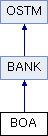
\includegraphics[height=3.000000cm]{class_b_o_a}
\end{center}
\end{figure}
\subsection*{Public Member Functions}
\begin{DoxyCompactItemize}
\item 
{\bf B\+OA} ()
\item 
{\bf B\+OA} (int account\+Number, double balance, std\+::string first\+Name, std\+::string last\+Name, std\+::string address)
\item 
{\bf B\+OA} (std\+::shared\+\_\+ptr$<$ {\bf B\+A\+NK} $>$ obj, int \+\_\+version, int \+\_\+unique\+\_\+id)
\item 
{\bf B\+OA} (const {\bf B\+OA} \&orig)
\item 
{\bf B\+OA} {\bf operator=} (const {\bf B\+OA} \&orig)
\item 
virtual {\bf $\sim$\+B\+OA} ()
\item 
virtual void {\bf copy} (std\+::shared\+\_\+ptr$<$ {\bf O\+S\+TM} $>$ to, std\+::shared\+\_\+ptr$<$ {\bf O\+S\+TM} $>$ from)
\begin{DoxyCompactList}\small\item\em copy function, make deep copy of the object/pointer \end{DoxyCompactList}\item 
virtual std\+::shared\+\_\+ptr$<$ {\bf O\+S\+TM} $>$ {\bf get\+Base\+Copy} (std\+::shared\+\_\+ptr$<$ {\bf O\+S\+TM} $>$ object)
\begin{DoxyCompactList}\small\item\em get\+Base\+Copy function, make deep copy of the object/pointer and Return a new std\+::shared\+\_\+ptr$<$\+B\+A\+N\+K$>$ type object \end{DoxyCompactList}\item 
virtual void {\bf to\+String} ()
\begin{DoxyCompactList}\small\item\em \+\_\+cast, is use to cast bak the std\+::shared\+\_\+ptr$<$\+O\+S\+T\+M$>$ to the required type \end{DoxyCompactList}\item 
virtual void {\bfseries Set\+Address} (std\+::string address)\label{class_b_o_a_a2568c0027af6534bd08dde882e892caf}

\item 
virtual std\+::string {\bfseries Get\+Address} () const \label{class_b_o_a_aa4aa2cf1ef0e876bb7911c00b5374493}

\item 
virtual void {\bfseries Set\+Balance} (double balance)\label{class_b_o_a_a0e06a7b7669b6a26a41b37d68f0a87b8}

\item 
virtual double {\bfseries Get\+Balance} () const \label{class_b_o_a_a07e30b7e5f5f20392b94af7344fd550c}

\item 
virtual void {\bfseries Set\+Account\+Number} (int account\+Number)\label{class_b_o_a_a6b85963680344bd719ab862a50a09588}

\item 
virtual int {\bfseries Get\+Account\+Number} () const \label{class_b_o_a_ad64bd63675f8902153aa6767994f05dc}

\item 
virtual void {\bfseries Set\+Last\+Name} (std\+::string last\+Name)\label{class_b_o_a_a7ea44308c05532cd11ff3ce8f14ea4c2}

\item 
virtual std\+::string {\bfseries Get\+Last\+Name} () const \label{class_b_o_a_a081383edefc1f66b80c3fb8862ab070b}

\item 
virtual void {\bfseries Set\+First\+Name} (std\+::string first\+Name)\label{class_b_o_a_a32fabc2b3acde832f3749696b302a0fe}

\item 
virtual std\+::string {\bfseries Get\+First\+Name} () const \label{class_b_o_a_ae6bb3df4e1fb210610325ffd1985c7c0}

\item 
virtual void {\bfseries Set\+Fullname} (std\+::string fullname)\label{class_b_o_a_a7ff134d56805088f46df8eb6f21a0a45}

\item 
virtual std\+::string {\bfseries Get\+Fullname} () const \label{class_b_o_a_afafa24a20fda93382782cab66a3079ee}

\end{DoxyCompactItemize}


\subsection{Detailed Description}
Inherit from \doxyref{B\+A\+NK}{p.}{class_b_a_n_k} 

Definition at line 18 of file B\+O\+A.\+h.



\subsection{Constructor \& Destructor Documentation}
\index{B\+OA@{B\+OA}!B\+OA@{B\+OA}}
\index{B\+OA@{B\+OA}!B\+OA@{B\+OA}}
\subsubsection[{B\+O\+A()}]{\setlength{\rightskip}{0pt plus 5cm}B\+O\+A\+::\+B\+OA (
\begin{DoxyParamCaption}
{}
\end{DoxyParamCaption}
)\hspace{0.3cm}{\ttfamily [inline]}}\label{class_b_o_a_ad42dc670d422172c9bcf9b3d354c8a3c}
Constructor 

Definition at line 24 of file B\+O\+A.\+h.

\index{B\+OA@{B\+OA}!B\+OA@{B\+OA}}
\index{B\+OA@{B\+OA}!B\+OA@{B\+OA}}
\subsubsection[{B\+O\+A(int account\+Number, double balance, std\+::string first\+Name, std\+::string last\+Name, std\+::string address)}]{\setlength{\rightskip}{0pt plus 5cm}B\+O\+A\+::\+B\+OA (
\begin{DoxyParamCaption}
\item[{int}]{account\+Number, }
\item[{double}]{balance, }
\item[{std\+::string}]{first\+Name, }
\item[{std\+::string}]{last\+Name, }
\item[{std\+::string}]{address}
\end{DoxyParamCaption}
)\hspace{0.3cm}{\ttfamily [inline]}}\label{class_b_o_a_a898c8627b8976bbe1a7d0fc780642b25}
Custom constructor 

Definition at line 35 of file B\+O\+A.\+h.

\index{B\+OA@{B\+OA}!B\+OA@{B\+OA}}
\index{B\+OA@{B\+OA}!B\+OA@{B\+OA}}
\subsubsection[{B\+O\+A(std\+::shared\+\_\+ptr$<$ B\+A\+N\+K $>$ obj, int \+\_\+version, int \+\_\+unique\+\_\+id)}]{\setlength{\rightskip}{0pt plus 5cm}B\+O\+A\+::\+B\+OA (
\begin{DoxyParamCaption}
\item[{std\+::shared\+\_\+ptr$<$ {\bf B\+A\+NK} $>$}]{obj, }
\item[{int}]{\+\_\+version, }
\item[{int}]{\+\_\+unique\+\_\+id}
\end{DoxyParamCaption}
)\hspace{0.3cm}{\ttfamily [inline]}}\label{class_b_o_a_ab87192ed986e601c2eb682ea3745daf0}
Custom constructor, used by the library for deep copying 

Definition at line 46 of file B\+O\+A.\+h.

\index{B\+OA@{B\+OA}!B\+OA@{B\+OA}}
\index{B\+OA@{B\+OA}!B\+OA@{B\+OA}}
\subsubsection[{B\+O\+A(const B\+O\+A \&orig)}]{\setlength{\rightskip}{0pt plus 5cm}B\+O\+A\+::\+B\+OA (
\begin{DoxyParamCaption}
\item[{const {\bf B\+OA} \&}]{orig}
\end{DoxyParamCaption}
)}\label{class_b_o_a_a99ebf22a8d824761dc82e7e191e6f173}
Copy constructor 

Definition at line 12 of file B\+O\+A.\+cpp.

\index{B\+OA@{B\+OA}!````~B\+OA@{$\sim$\+B\+OA}}
\index{````~B\+OA@{$\sim$\+B\+OA}!B\+OA@{B\+OA}}
\subsubsection[{$\sim$\+B\+O\+A()}]{\setlength{\rightskip}{0pt plus 5cm}B\+O\+A\+::$\sim$\+B\+OA (
\begin{DoxyParamCaption}
{}
\end{DoxyParamCaption}
)\hspace{0.3cm}{\ttfamily [virtual]}}\label{class_b_o_a_abe27b17a23ceffc6269dbe6d81de5212}
de-\/constructor 

Definition at line 15 of file B\+O\+A.\+cpp.



\subsection{Member Function Documentation}
\index{B\+OA@{B\+OA}!copy@{copy}}
\index{copy@{copy}!B\+OA@{B\+OA}}
\subsubsection[{copy(std\+::shared\+\_\+ptr$<$ O\+S\+T\+M $>$ to, std\+::shared\+\_\+ptr$<$ O\+S\+T\+M $>$ from)}]{\setlength{\rightskip}{0pt plus 5cm}void B\+O\+A\+::copy (
\begin{DoxyParamCaption}
\item[{std\+::shared\+\_\+ptr$<$ {\bf O\+S\+TM} $>$}]{to, }
\item[{std\+::shared\+\_\+ptr$<$ {\bf O\+S\+TM} $>$}]{from}
\end{DoxyParamCaption}
)\hspace{0.3cm}{\ttfamily [virtual]}}\label{class_b_o_a_a54fbcabb55b22fb72f45986768974403}


copy function, make deep copy of the object/pointer 


\begin{DoxyParams}{Parameters}
{\em obj\+TO} & is a std\+::shared\+\_\+ptr$<$\+B\+A\+N\+K$>$ type object casted back from std\+::shared\+\_\+ptr$<$\+O\+S\+T\+M$>$ \\
\hline
{\em obj\+F\+R\+OM} & is a std\+::shared\+\_\+ptr$<$\+B\+A\+N\+K$>$ type object casted back from std\+::shared\+\_\+ptr$<$\+O\+S\+T\+M$>$ \\
\hline
\end{DoxyParams}


Reimplemented from {\bf O\+S\+TM} \doxyref{}{p.}{class_o_s_t_m_a535d90fced5adbb70312c92f3778e08d}.



Definition at line 34 of file B\+O\+A.\+cpp.

\index{B\+OA@{B\+OA}!get\+Base\+Copy@{get\+Base\+Copy}}
\index{get\+Base\+Copy@{get\+Base\+Copy}!B\+OA@{B\+OA}}
\subsubsection[{get\+Base\+Copy(std\+::shared\+\_\+ptr$<$ O\+S\+T\+M $>$ object)}]{\setlength{\rightskip}{0pt plus 5cm}std\+::shared\+\_\+ptr$<$ {\bf O\+S\+TM} $>$ B\+O\+A\+::get\+Base\+Copy (
\begin{DoxyParamCaption}
\item[{std\+::shared\+\_\+ptr$<$ {\bf O\+S\+TM} $>$}]{object}
\end{DoxyParamCaption}
)\hspace{0.3cm}{\ttfamily [virtual]}}\label{class_b_o_a_a46ace5d3c945a423e93912673cadfad5}


get\+Base\+Copy function, make deep copy of the object/pointer and Return a new std\+::shared\+\_\+ptr$<$\+B\+A\+N\+K$>$ type object 


\begin{DoxyParams}{Parameters}
{\em obj\+TO} & is a \doxyref{B\+A\+NK}{p.}{class_b_a_n_k} type pointer for casting \\
\hline
{\em obj} & is a std\+::shared\+\_\+ptr$<$\+B\+A\+N\+K$>$ return type \\
\hline
\end{DoxyParams}


Reimplemented from {\bf O\+S\+TM} \doxyref{}{p.}{class_o_s_t_m_a0bfa3763bd441407dd6365f42714f94c}.



Definition at line 22 of file B\+O\+A.\+cpp.

\index{B\+OA@{B\+OA}!operator=@{operator=}}
\index{operator=@{operator=}!B\+OA@{B\+OA}}
\subsubsection[{operator=(const B\+O\+A \&orig)}]{\setlength{\rightskip}{0pt plus 5cm}{\bf B\+OA} B\+O\+A\+::operator= (
\begin{DoxyParamCaption}
\item[{const {\bf B\+OA} \&}]{orig}
\end{DoxyParamCaption}
)\hspace{0.3cm}{\ttfamily [inline]}}\label{class_b_o_a_af24b66f0e072b29abbbe5812cab48369}
Operator 

Definition at line 64 of file B\+O\+A.\+h.

\index{B\+OA@{B\+OA}!to\+String@{to\+String}}
\index{to\+String@{to\+String}!B\+OA@{B\+OA}}
\subsubsection[{to\+String()}]{\setlength{\rightskip}{0pt plus 5cm}void B\+O\+A\+::to\+String (
\begin{DoxyParamCaption}
{}
\end{DoxyParamCaption}
)\hspace{0.3cm}{\ttfamily [virtual]}}\label{class_b_o_a_a348df0299997f81bcad0ec034dab0b8d}


\+\_\+cast, is use to cast bak the std\+::shared\+\_\+ptr$<$\+O\+S\+T\+M$>$ to the required type 

to\+String function, displays the object values in formatted way 

Reimplemented from {\bf O\+S\+TM} \doxyref{}{p.}{class_o_s_t_m_a513396a115f2987fd07c203309ae8a59}.



Definition at line 54 of file B\+O\+A.\+cpp.



The documentation for this class was generated from the following files\+:\begin{DoxyCompactItemize}
\item 
/media/zoltan/\+Data/00\+\_\+2018\+\_\+\+I\+T\+Carlow/00\+\_\+\+Modules/06\+\_\+\+Project/\+Documents/\+Git\+\_\+\+Sync/\+Main Tests for Linux/\+Test01/B\+O\+A.\+h\item 
/media/zoltan/\+Data/00\+\_\+2018\+\_\+\+I\+T\+Carlow/00\+\_\+\+Modules/06\+\_\+\+Project/\+Documents/\+Git\+\_\+\+Sync/\+Main Tests for Linux/\+Test01/B\+O\+A.\+cpp\end{DoxyCompactItemize}

\hypertarget{class_b_o_i}{}\subsection{B\+OI Class Reference}
\label{class_b_o_i}\index{B\+OI@{B\+OI}}


{\ttfamily \#include $<$B\+O\+I.\+h$>$}



Inheritance diagram for B\+OI\+:
\nopagebreak
\begin{figure}[H]
\begin{center}
\leavevmode
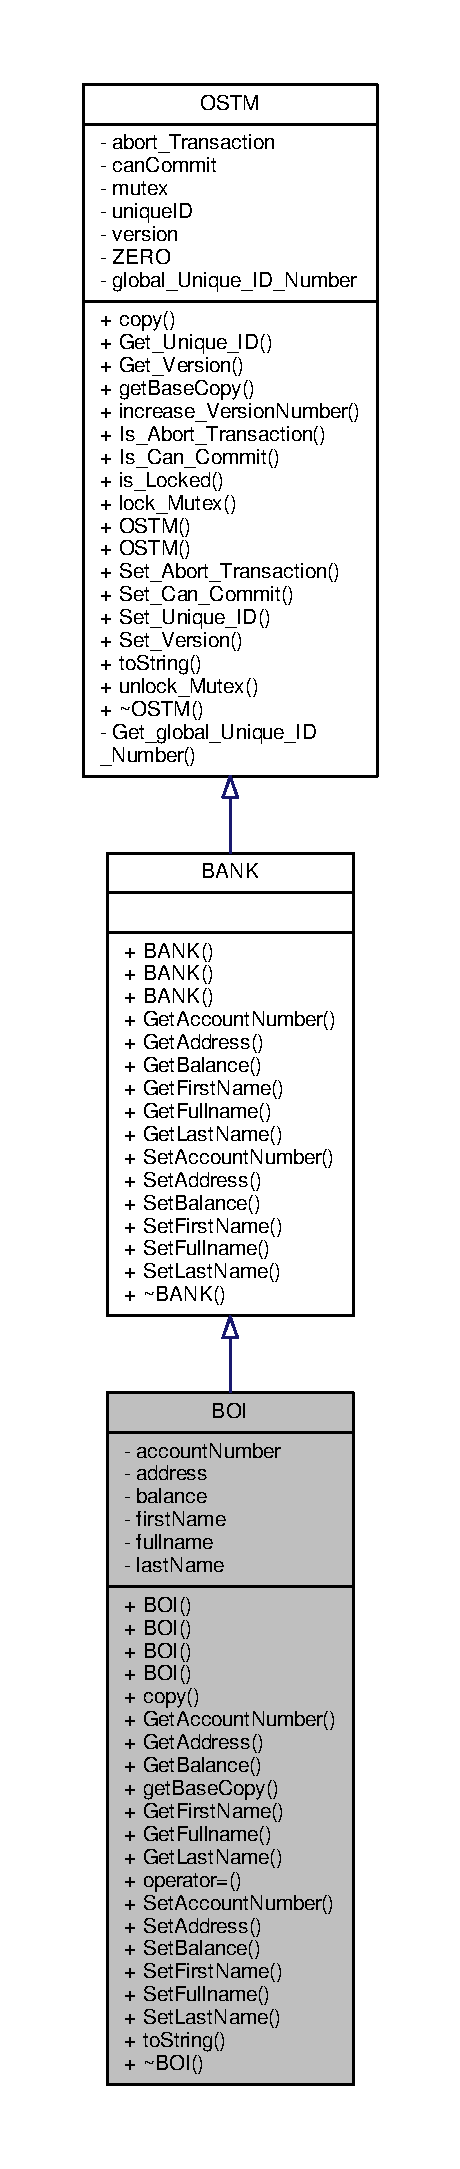
\includegraphics[width=198pt]{class_b_o_i__inherit__graph}
\end{center}
\end{figure}


Collaboration diagram for B\+OI\+:
\nopagebreak
\begin{figure}[H]
\begin{center}
\leavevmode
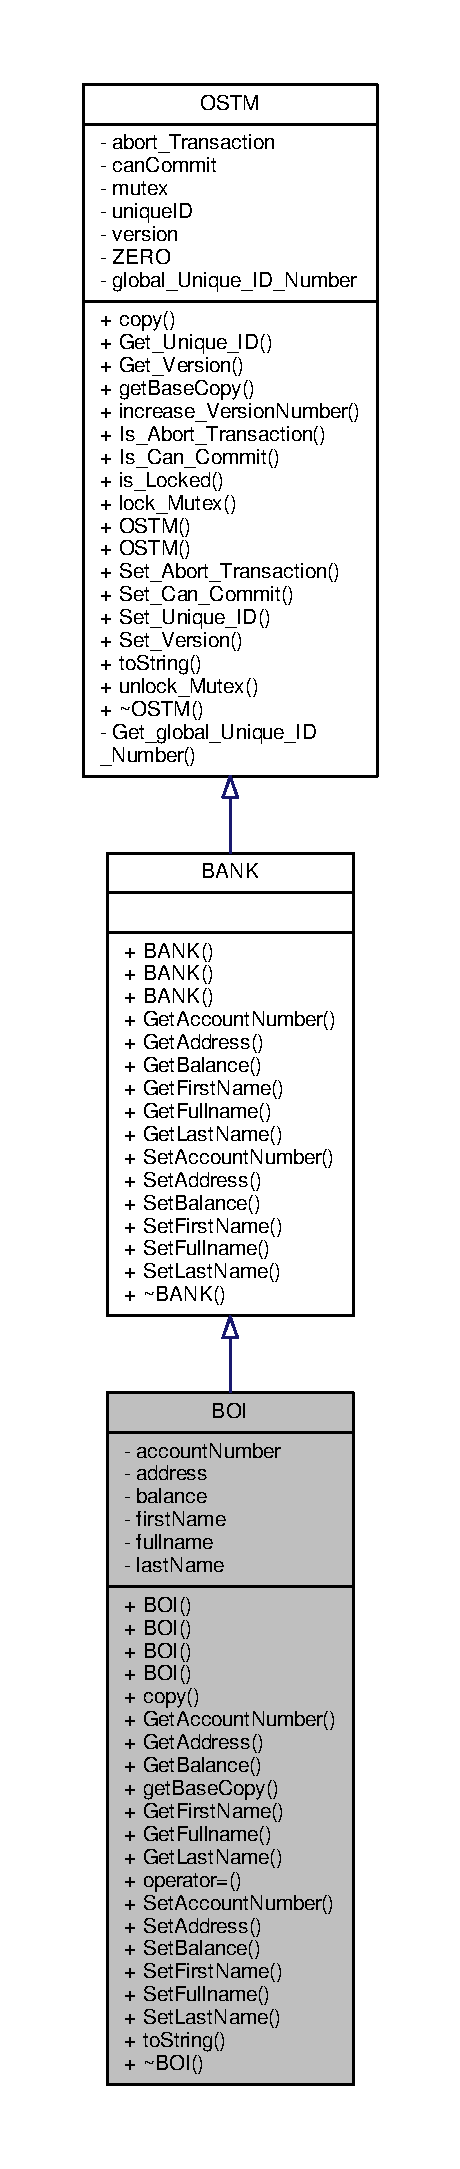
\includegraphics[width=198pt]{class_b_o_i__coll__graph}
\end{center}
\end{figure}
\subsubsection*{Public Member Functions}
\begin{DoxyCompactItemize}
\item 
\hyperlink{class_b_o_i_a6af682a5f199a029681f0cb2b8658706}{B\+OI} ()
\item 
\hyperlink{class_b_o_i_a1807bd07cad08109c974edbb2c32591c}{B\+OI} (int account\+Number, double balance, std\+::string first\+Name, std\+::string last\+Name, std\+::string address)
\item 
\hyperlink{class_b_o_i_ae4263940f8ffdd40d5f01a714b20f791}{B\+OI} (std\+::shared\+\_\+ptr$<$ \hyperlink{class_b_o_i}{B\+OI} $>$ obj, int \+\_\+version, int \+\_\+unique\+\_\+id)
\item 
\hyperlink{class_b_o_i_a7757de8d3ac656871bed4b07d77457ff}{B\+OI} (const \hyperlink{class_b_o_i}{B\+OI} \&orig)
\item 
\hyperlink{class_b_o_i}{B\+OI} \hyperlink{class_b_o_i_a4b4a3976cc13c4d3de0d7ff8882a7af3}{operator=} (const \hyperlink{class_b_o_i}{B\+OI} \&orig)
\item 
virtual \hyperlink{class_b_o_i_a617f46a599129178c6b11b4846759a6c}{$\sim$\+B\+OI} ()
\item 
virtual std\+::shared\+\_\+ptr$<$ O\+S\+TM $>$ \hyperlink{class_b_o_i_ad53ae2918a656793b9d7a670d35ecfa3}{get\+Base\+Copy} (std\+::shared\+\_\+ptr$<$ O\+S\+TM $>$ object)
\begin{DoxyCompactList}\small\item\em get\+Base\+Copy function, make deep copy of the object/pointer and Return a new B\+A\+N\+K$\ast$ type object \end{DoxyCompactList}\item 
virtual void \hyperlink{class_b_o_i_a9ff2d32c25c23a1bea6316f50c3bf677}{copy} (std\+::shared\+\_\+ptr$<$ O\+S\+TM $>$ to, std\+::shared\+\_\+ptr$<$ O\+S\+TM $>$ from)
\begin{DoxyCompactList}\small\item\em copy function, make deep copy of the object/pointer \end{DoxyCompactList}\item 
virtual void \hyperlink{class_b_o_i_ab02a4dd4ebcc5b2abfaca19f2dff2006}{to\+String} ()
\begin{DoxyCompactList}\small\item\em \+\_\+cast, is use to cast bak the std\+::shared\+\_\+ptr$<$\+O\+S\+T\+M$>$ to the required type \end{DoxyCompactList}\item 
virtual void \hyperlink{class_b_o_i_a00c9386c862cf2442968bf7fc30102b3}{Set\+Address} (std\+::string address)
\item 
virtual std\+::string \hyperlink{class_b_o_i_a8920e1f47b22445ba954e86012207462}{Get\+Address} () const 
\item 
virtual void \hyperlink{class_b_o_i_a416667693c10f5e4120eec97a9269348}{Set\+Balance} (double balance)
\item 
virtual double \hyperlink{class_b_o_i_a25b289dece2a1685bb9d1a9332c9be0b}{Get\+Balance} () const 
\item 
virtual void \hyperlink{class_b_o_i_affc9e7e2a36214b3790f250b7108bb65}{Set\+Account\+Number} (int account\+Number)
\item 
virtual int \hyperlink{class_b_o_i_a5b18e1538f3d37835234946cdf9f240f}{Get\+Account\+Number} () const 
\item 
virtual void \hyperlink{class_b_o_i_a663906e9a59ffa970fb928746c01e8af}{Set\+Last\+Name} (std\+::string last\+Name)
\item 
virtual std\+::string \hyperlink{class_b_o_i_a37828f3fa4a32f522966e2cad90eaab2}{Get\+Last\+Name} () const 
\item 
virtual void \hyperlink{class_b_o_i_ae9042f87be085c2cec799981c30d7d19}{Set\+First\+Name} (std\+::string first\+Name)
\item 
virtual std\+::string \hyperlink{class_b_o_i_ab4b9d50c6008a666aa4382def580e7d1}{Get\+First\+Name} () const 
\item 
virtual void \hyperlink{class_b_o_i_a93091f16610f1a1474aea31fd5f81ffd}{Set\+Fullname} (std\+::string fullname)
\item 
virtual std\+::string \hyperlink{class_b_o_i_af56446a377068cd65526e40e8b31b878}{Get\+Fullname} () const 
\end{DoxyCompactItemize}


\subsubsection{Detailed Description}
Inherit from \hyperlink{class_b_a_n_k}{B\+A\+NK} 

Definition at line \hyperlink{_b_o_i_8h_source_l00019}{19} of file \hyperlink{_b_o_i_8h_source}{B\+O\+I.\+h}.



\subsubsection{Constructor \& Destructor Documentation}
\index{B\+OI@{B\+OI}!B\+OI@{B\+OI}}
\index{B\+OI@{B\+OI}!B\+OI@{B\+OI}}
\paragraph[{\texorpdfstring{B\+O\+I()}{BOI()}}]{\setlength{\rightskip}{0pt plus 5cm}B\+O\+I\+::\+B\+OI (
\begin{DoxyParamCaption}
{}
\end{DoxyParamCaption}
)\hspace{0.3cm}{\ttfamily [inline]}}\hypertarget{class_b_o_i_a6af682a5f199a029681f0cb2b8658706}{}\label{class_b_o_i_a6af682a5f199a029681f0cb2b8658706}
Constructor 

Definition at line \hyperlink{_b_o_i_8h_source_l00024}{24} of file \hyperlink{_b_o_i_8h_source}{B\+O\+I.\+h}.



Referenced by \hyperlink{_b_o_i_8h_source_l00049}{B\+O\+I()}, and \hyperlink{_b_o_i_8cpp_source_l00022}{get\+Base\+Copy()}.


\begin{DoxyCode}
00024          : \hyperlink{class_b_a_n_k_a0bc938356cebff14fb0560264abe5a34}{BANK}()
00025     \{
00026         this->accountNumber = 0;
00027         this->balance = 50;
00028         this->firstName = \textcolor{stringliteral}{"Joe"};
00029         this->lastName = \textcolor{stringliteral}{"Blog"};
00030         this->address = \textcolor{stringliteral}{"High street, Carlow"};
00031         this->fullname = firstName + \textcolor{stringliteral}{" "} + lastName;
00032         
00033     \}
\end{DoxyCode}


Here is the caller graph for this function\+:\nopagebreak
\begin{figure}[H]
\begin{center}
\leavevmode
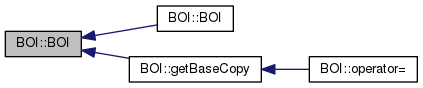
\includegraphics[width=350pt]{class_b_o_i_a6af682a5f199a029681f0cb2b8658706_icgraph}
\end{center}
\end{figure}


\index{B\+OI@{B\+OI}!B\+OI@{B\+OI}}
\index{B\+OI@{B\+OI}!B\+OI@{B\+OI}}
\paragraph[{\texorpdfstring{B\+O\+I(int account\+Number, double balance, std\+::string first\+Name, std\+::string last\+Name, std\+::string address)}{BOI(int accountNumber, double balance, std::string firstName, std::string lastName, std::string address)}}]{\setlength{\rightskip}{0pt plus 5cm}B\+O\+I\+::\+B\+OI (
\begin{DoxyParamCaption}
\item[{int}]{account\+Number, }
\item[{double}]{balance, }
\item[{std\+::string}]{first\+Name, }
\item[{std\+::string}]{last\+Name, }
\item[{std\+::string}]{address}
\end{DoxyParamCaption}
)\hspace{0.3cm}{\ttfamily [inline]}}\hypertarget{class_b_o_i_a1807bd07cad08109c974edbb2c32591c}{}\label{class_b_o_i_a1807bd07cad08109c974edbb2c32591c}
Custom constructor 

Definition at line \hyperlink{_b_o_i_8h_source_l00037}{37} of file \hyperlink{_b_o_i_8h_source}{B\+O\+I.\+h}.


\begin{DoxyCode}
00037                                                                                                       : 
      \hyperlink{class_b_a_n_k_a0bc938356cebff14fb0560264abe5a34}{BANK}()
00038     \{
00039         this->accountNumber = accountNumber;
00040         this->balance = balance;
00041         this->firstName = firstName;
00042         this->lastName = lastName;
00043         this->address = address;
00044         this->fullname = firstName + \textcolor{stringliteral}{" "} + lastName;
00045     \};
\end{DoxyCode}
\index{B\+OI@{B\+OI}!B\+OI@{B\+OI}}
\index{B\+OI@{B\+OI}!B\+OI@{B\+OI}}
\paragraph[{\texorpdfstring{B\+O\+I(std\+::shared\+\_\+ptr$<$ B\+O\+I $>$ obj, int \+\_\+version, int \+\_\+unique\+\_\+id)}{BOI(std::shared_ptr< BOI > obj, int _version, int _unique_id)}}]{\setlength{\rightskip}{0pt plus 5cm}B\+O\+I\+::\+B\+OI (
\begin{DoxyParamCaption}
\item[{std\+::shared\+\_\+ptr$<$ {\bf B\+OI} $>$}]{obj, }
\item[{int}]{\+\_\+version, }
\item[{int}]{\+\_\+unique\+\_\+id}
\end{DoxyParamCaption}
)\hspace{0.3cm}{\ttfamily [inline]}}\hypertarget{class_b_o_i_ae4263940f8ffdd40d5f01a714b20f791}{}\label{class_b_o_i_ae4263940f8ffdd40d5f01a714b20f791}
Custom constructor, used by the library for deep copying 

Definition at line \hyperlink{_b_o_i_8h_source_l00049}{49} of file \hyperlink{_b_o_i_8h_source}{B\+O\+I.\+h}.



References \hyperlink{_b_o_i_8h_source_l00024}{B\+O\+I()}.


\begin{DoxyCode}
00049                                                              : \hyperlink{class_b_a_n_k_a0bc938356cebff14fb0560264abe5a34}{BANK}(\_version, \_unique\_id)
00050     \{
00051         this->accountNumber = obj->GetAccountNumber();
00052         this->balance = obj->GetBalance();
00053         this->firstName = obj->GetFirstName();
00054         this->lastName = obj->GetLastName();
00055         this->address = obj->GetAddress();
00056         this->fullname = obj->GetFirstName() + \textcolor{stringliteral}{" "} + obj->GetLastName(); 
00057     \};
\end{DoxyCode}


Here is the call graph for this function\+:\nopagebreak
\begin{figure}[H]
\begin{center}
\leavevmode
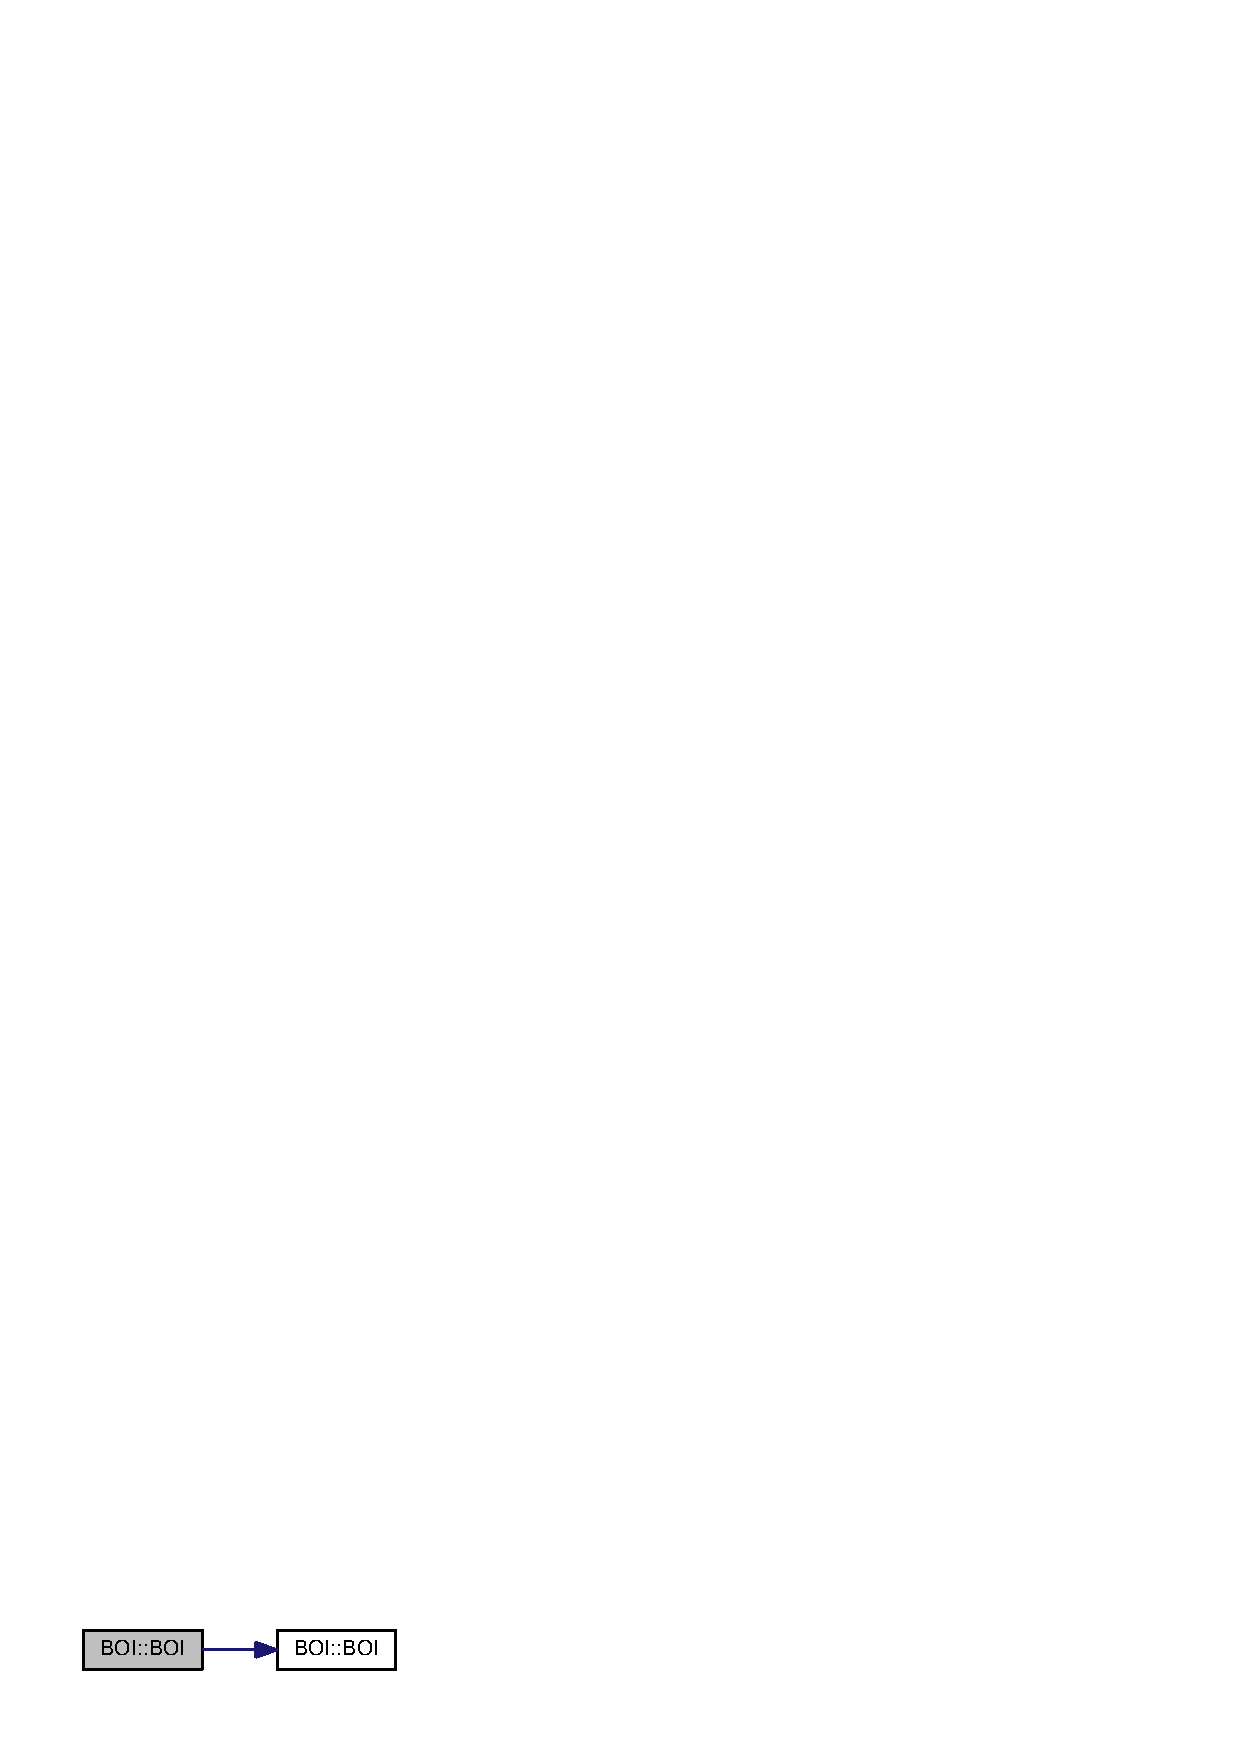
\includegraphics[width=230pt]{class_b_o_i_ae4263940f8ffdd40d5f01a714b20f791_cgraph}
\end{center}
\end{figure}


\index{B\+OI@{B\+OI}!B\+OI@{B\+OI}}
\index{B\+OI@{B\+OI}!B\+OI@{B\+OI}}
\paragraph[{\texorpdfstring{B\+O\+I(const B\+O\+I \&orig)}{BOI(const BOI &orig)}}]{\setlength{\rightskip}{0pt plus 5cm}B\+O\+I\+::\+B\+OI (
\begin{DoxyParamCaption}
\item[{const {\bf B\+OI} \&}]{orig}
\end{DoxyParamCaption}
)}\hypertarget{class_b_o_i_a7757de8d3ac656871bed4b07d77457ff}{}\label{class_b_o_i_a7757de8d3ac656871bed4b07d77457ff}
Copy constructor 

Definition at line \hyperlink{_b_o_i_8cpp_source_l00015}{15} of file \hyperlink{_b_o_i_8cpp_source}{B\+O\+I.\+cpp}.


\begin{DoxyCode}
00015                         \{
00016 \}
\end{DoxyCode}
\index{B\+OI@{B\+OI}!````~B\+OI@{$\sim$\+B\+OI}}
\index{````~B\+OI@{$\sim$\+B\+OI}!B\+OI@{B\+OI}}
\paragraph[{\texorpdfstring{$\sim$\+B\+O\+I()}{~BOI()}}]{\setlength{\rightskip}{0pt plus 5cm}B\+O\+I\+::$\sim$\+B\+OI (
\begin{DoxyParamCaption}
{}
\end{DoxyParamCaption}
)\hspace{0.3cm}{\ttfamily [virtual]}}\hypertarget{class_b_o_i_a617f46a599129178c6b11b4846759a6c}{}\label{class_b_o_i_a617f46a599129178c6b11b4846759a6c}
de-\/constructor 

Definition at line \hyperlink{_b_o_i_8cpp_source_l00012}{12} of file \hyperlink{_b_o_i_8cpp_source}{B\+O\+I.\+cpp}.



Referenced by \hyperlink{_b_o_i_8h_source_l00065}{operator=()}.


\begin{DoxyCode}
00012           \{
00013 \}
\end{DoxyCode}


Here is the caller graph for this function\+:\nopagebreak
\begin{figure}[H]
\begin{center}
\leavevmode
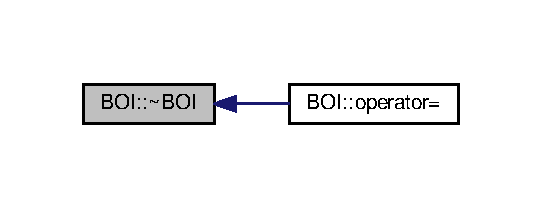
\includegraphics[width=260pt]{class_b_o_i_a617f46a599129178c6b11b4846759a6c_icgraph}
\end{center}
\end{figure}




\subsubsection{Member Function Documentation}
\index{B\+OI@{B\+OI}!copy@{copy}}
\index{copy@{copy}!B\+OI@{B\+OI}}
\paragraph[{\texorpdfstring{copy(std\+::shared\+\_\+ptr$<$ O\+S\+T\+M $>$ to, std\+::shared\+\_\+ptr$<$ O\+S\+T\+M $>$ from)}{copy(std::shared_ptr< OSTM > to, std::shared_ptr< OSTM > from)}}]{\setlength{\rightskip}{0pt plus 5cm}void B\+O\+I\+::copy (
\begin{DoxyParamCaption}
\item[{std\+::shared\+\_\+ptr$<$ O\+S\+TM $>$}]{to, }
\item[{std\+::shared\+\_\+ptr$<$ O\+S\+TM $>$}]{from}
\end{DoxyParamCaption}
)\hspace{0.3cm}{\ttfamily [virtual]}}\hypertarget{class_b_o_i_a9ff2d32c25c23a1bea6316f50c3bf677}{}\label{class_b_o_i_a9ff2d32c25c23a1bea6316f50c3bf677}


copy function, make deep copy of the object/pointer 


\begin{DoxyParams}{Parameters}
{\em obj\+TO} & is a B\+A\+N\+K$\ast$ type object casted back from std\+::shared\+\_\+ptr$<$\+O\+S\+T\+M$>$ \\
\hline
{\em obj\+F\+R\+OM} & is a B\+A\+N\+K$\ast$ type object casted back from std\+::shared\+\_\+ptr$<$\+O\+S\+T\+M$>$ \\
\hline
\end{DoxyParams}


Definition at line \hyperlink{_b_o_i_8cpp_source_l00035}{35} of file \hyperlink{_b_o_i_8cpp_source}{B\+O\+I.\+cpp}.



References \hyperlink{_b_o_i_8cpp_source_l00074}{Set\+Account\+Number()}.



Referenced by \hyperlink{_b_o_i_8h_source_l00065}{operator=()}.


\begin{DoxyCode}
00035                                                               \{
00036 
00037     std::shared\_ptr<BOI> objTO = std::dynamic\_pointer\_cast<\hyperlink{class_b_o_i}{BOI}>(to);
00038     std::shared\_ptr<BOI> objFROM = std::dynamic\_pointer\_cast<\hyperlink{class_b_o_i}{BOI}>(from);
00039     objTO->Set\_Unique\_ID(objFROM->Get\_Unique\_ID());
00040     objTO->Set\_Version(objFROM->Get\_Version());
00041     objTO->\hyperlink{class_b_o_i_affc9e7e2a36214b3790f250b7108bb65}{SetAccountNumber}(objFROM->GetAccountNumber());
00042     objTO->SetBalance(objFROM->GetBalance());
00043 \}
\end{DoxyCode}


Here is the call graph for this function\+:\nopagebreak
\begin{figure}[H]
\begin{center}
\leavevmode
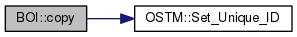
\includegraphics[width=302pt]{class_b_o_i_a9ff2d32c25c23a1bea6316f50c3bf677_cgraph}
\end{center}
\end{figure}




Here is the caller graph for this function\+:\nopagebreak
\begin{figure}[H]
\begin{center}
\leavevmode
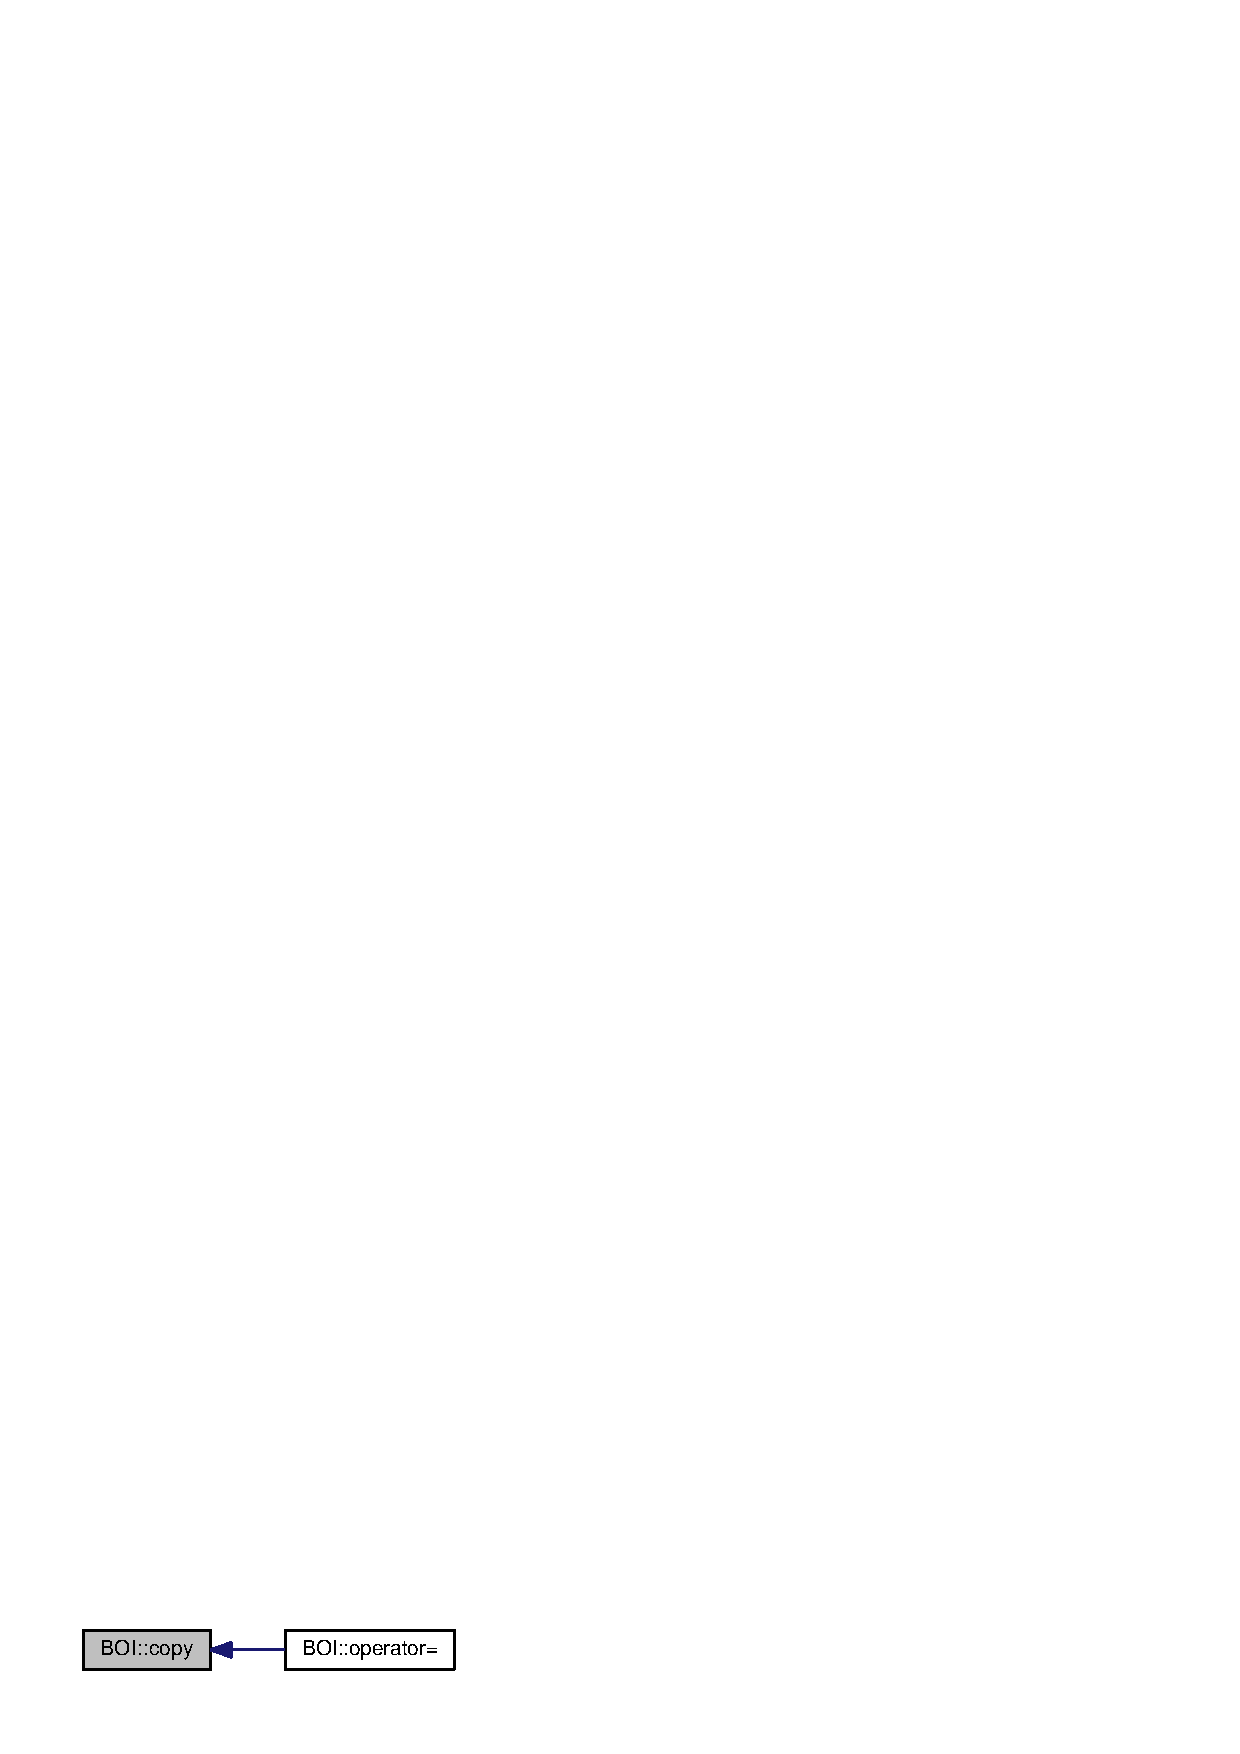
\includegraphics[width=258pt]{class_b_o_i_a9ff2d32c25c23a1bea6316f50c3bf677_icgraph}
\end{center}
\end{figure}


\index{B\+OI@{B\+OI}!Get\+Account\+Number@{Get\+Account\+Number}}
\index{Get\+Account\+Number@{Get\+Account\+Number}!B\+OI@{B\+OI}}
\paragraph[{\texorpdfstring{Get\+Account\+Number() const }{GetAccountNumber() const }}]{\setlength{\rightskip}{0pt plus 5cm}int B\+O\+I\+::\+Get\+Account\+Number (
\begin{DoxyParamCaption}
{}
\end{DoxyParamCaption}
) const\hspace{0.3cm}{\ttfamily [virtual]}}\hypertarget{class_b_o_i_a5b18e1538f3d37835234946cdf9f240f}{}\label{class_b_o_i_a5b18e1538f3d37835234946cdf9f240f}


Implements \hyperlink{class_b_a_n_k_a781f774d1b3fd7437563811b015cbc8c}{B\+A\+NK}.



Definition at line \hyperlink{_b_o_i_8cpp_source_l00078}{78} of file \hyperlink{_b_o_i_8cpp_source}{B\+O\+I.\+cpp}.



Referenced by \hyperlink{_b_o_i_8h_source_l00065}{operator=()}, and \hyperlink{_b_o_i_8cpp_source_l00054}{to\+String()}.


\begin{DoxyCode}
00078                                 \{
00079     \textcolor{keywordflow}{return} accountNumber;
00080 \}
\end{DoxyCode}


Here is the caller graph for this function\+:\nopagebreak
\begin{figure}[H]
\begin{center}
\leavevmode
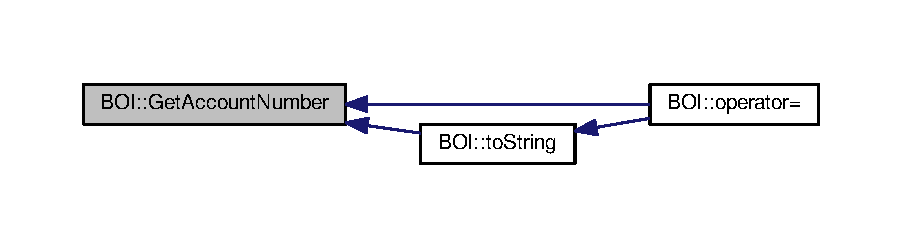
\includegraphics[width=350pt]{class_b_o_i_a5b18e1538f3d37835234946cdf9f240f_icgraph}
\end{center}
\end{figure}


\index{B\+OI@{B\+OI}!Get\+Address@{Get\+Address}}
\index{Get\+Address@{Get\+Address}!B\+OI@{B\+OI}}
\paragraph[{\texorpdfstring{Get\+Address() const }{GetAddress() const }}]{\setlength{\rightskip}{0pt plus 5cm}std\+::string B\+O\+I\+::\+Get\+Address (
\begin{DoxyParamCaption}
{}
\end{DoxyParamCaption}
) const\hspace{0.3cm}{\ttfamily [virtual]}}\hypertarget{class_b_o_i_a8920e1f47b22445ba954e86012207462}{}\label{class_b_o_i_a8920e1f47b22445ba954e86012207462}


Implements \hyperlink{class_b_a_n_k_af1847278d240ceb2b831f03c7e039e07}{B\+A\+NK}.



Definition at line \hyperlink{_b_o_i_8cpp_source_l00062}{62} of file \hyperlink{_b_o_i_8cpp_source}{B\+O\+I.\+cpp}.



Referenced by \hyperlink{_b_o_i_8h_source_l00065}{operator=()}.


\begin{DoxyCode}
00062                                 \{
00063     \textcolor{keywordflow}{return} address;
00064 \}
\end{DoxyCode}


Here is the caller graph for this function\+:\nopagebreak
\begin{figure}[H]
\begin{center}
\leavevmode
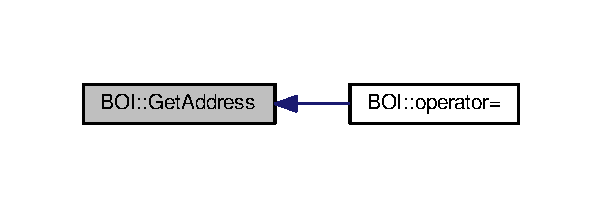
\includegraphics[width=289pt]{class_b_o_i_a8920e1f47b22445ba954e86012207462_icgraph}
\end{center}
\end{figure}


\index{B\+OI@{B\+OI}!Get\+Balance@{Get\+Balance}}
\index{Get\+Balance@{Get\+Balance}!B\+OI@{B\+OI}}
\paragraph[{\texorpdfstring{Get\+Balance() const }{GetBalance() const }}]{\setlength{\rightskip}{0pt plus 5cm}double B\+O\+I\+::\+Get\+Balance (
\begin{DoxyParamCaption}
{}
\end{DoxyParamCaption}
) const\hspace{0.3cm}{\ttfamily [virtual]}}\hypertarget{class_b_o_i_a25b289dece2a1685bb9d1a9332c9be0b}{}\label{class_b_o_i_a25b289dece2a1685bb9d1a9332c9be0b}


Implements \hyperlink{class_b_a_n_k_ae0fc62108895cddad418b23cb6d15f58}{B\+A\+NK}.



Definition at line \hyperlink{_b_o_i_8cpp_source_l00070}{70} of file \hyperlink{_b_o_i_8cpp_source}{B\+O\+I.\+cpp}.



Referenced by \hyperlink{_b_o_i_8h_source_l00065}{operator=()}, and \hyperlink{_b_o_i_8cpp_source_l00054}{to\+String()}.


\begin{DoxyCode}
00070                              \{
00071     \textcolor{keywordflow}{return} balance;
00072 \}
\end{DoxyCode}


Here is the caller graph for this function\+:\nopagebreak
\begin{figure}[H]
\begin{center}
\leavevmode
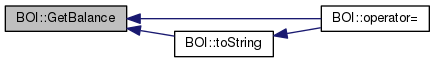
\includegraphics[width=350pt]{class_b_o_i_a25b289dece2a1685bb9d1a9332c9be0b_icgraph}
\end{center}
\end{figure}


\index{B\+OI@{B\+OI}!get\+Base\+Copy@{get\+Base\+Copy}}
\index{get\+Base\+Copy@{get\+Base\+Copy}!B\+OI@{B\+OI}}
\paragraph[{\texorpdfstring{get\+Base\+Copy(std\+::shared\+\_\+ptr$<$ O\+S\+T\+M $>$ object)}{getBaseCopy(std::shared_ptr< OSTM > object)}}]{\setlength{\rightskip}{0pt plus 5cm}std\+::shared\+\_\+ptr$<$ O\+S\+TM $>$ B\+O\+I\+::get\+Base\+Copy (
\begin{DoxyParamCaption}
\item[{std\+::shared\+\_\+ptr$<$ O\+S\+TM $>$}]{object}
\end{DoxyParamCaption}
)\hspace{0.3cm}{\ttfamily [virtual]}}\hypertarget{class_b_o_i_ad53ae2918a656793b9d7a670d35ecfa3}{}\label{class_b_o_i_ad53ae2918a656793b9d7a670d35ecfa3}


get\+Base\+Copy function, make deep copy of the object/pointer and Return a new B\+A\+N\+K$\ast$ type object 


\begin{DoxyParams}{Parameters}
{\em obj\+TO} & is a \hyperlink{class_b_a_n_k}{B\+A\+NK} type pointer for casting \\
\hline
{\em obj} & is a B\+A\+N\+K$\ast$ return type \\
\hline
\end{DoxyParams}


Definition at line \hyperlink{_b_o_i_8cpp_source_l00022}{22} of file \hyperlink{_b_o_i_8cpp_source}{B\+O\+I.\+cpp}.



References \hyperlink{_b_o_i_8h_source_l00024}{B\+O\+I()}.



Referenced by \hyperlink{_b_o_i_8h_source_l00065}{operator=()}.


\begin{DoxyCode}
00023 \{
00024 
00025     std::shared\_ptr<BOI> objTO = std::dynamic\_pointer\_cast<\hyperlink{class_b_o_i}{BOI}>(object);
00026     std::shared\_ptr<BOI> obj(\textcolor{keyword}{new} \hyperlink{class_b_o_i_a6af682a5f199a029681f0cb2b8658706}{BOI}(objTO,object->Get\_Version(),\textcolor{keywordtype}{object}->Get\_Unique\_ID())); 
00027     std::shared\_ptr<OSTM> ostm\_obj = std::dynamic\_pointer\_cast<OSTM>(obj);
00028     \textcolor{keywordflow}{return} ostm\_obj;
00029 \}
\end{DoxyCode}


Here is the call graph for this function\+:\nopagebreak
\begin{figure}[H]
\begin{center}
\leavevmode
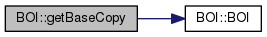
\includegraphics[width=272pt]{class_b_o_i_ad53ae2918a656793b9d7a670d35ecfa3_cgraph}
\end{center}
\end{figure}




Here is the caller graph for this function\+:\nopagebreak
\begin{figure}[H]
\begin{center}
\leavevmode
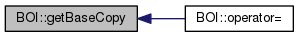
\includegraphics[width=296pt]{class_b_o_i_ad53ae2918a656793b9d7a670d35ecfa3_icgraph}
\end{center}
\end{figure}


\index{B\+OI@{B\+OI}!Get\+First\+Name@{Get\+First\+Name}}
\index{Get\+First\+Name@{Get\+First\+Name}!B\+OI@{B\+OI}}
\paragraph[{\texorpdfstring{Get\+First\+Name() const }{GetFirstName() const }}]{\setlength{\rightskip}{0pt plus 5cm}std\+::string B\+O\+I\+::\+Get\+First\+Name (
\begin{DoxyParamCaption}
{}
\end{DoxyParamCaption}
) const\hspace{0.3cm}{\ttfamily [virtual]}}\hypertarget{class_b_o_i_ab4b9d50c6008a666aa4382def580e7d1}{}\label{class_b_o_i_ab4b9d50c6008a666aa4382def580e7d1}


Implements \hyperlink{class_b_a_n_k_a6b50fbebbe0d807ff3bc36ad6dbe01b8}{B\+A\+NK}.



Definition at line \hyperlink{_b_o_i_8cpp_source_l00094}{94} of file \hyperlink{_b_o_i_8cpp_source}{B\+O\+I.\+cpp}.



Referenced by \hyperlink{_b_o_i_8h_source_l00065}{operator=()}, and \hyperlink{_b_o_i_8cpp_source_l00054}{to\+String()}.


\begin{DoxyCode}
00094                                   \{
00095     \textcolor{keywordflow}{return} firstName;
00096 \}
\end{DoxyCode}


Here is the caller graph for this function\+:\nopagebreak
\begin{figure}[H]
\begin{center}
\leavevmode
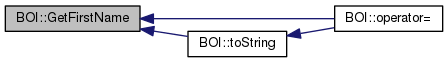
\includegraphics[width=350pt]{class_b_o_i_ab4b9d50c6008a666aa4382def580e7d1_icgraph}
\end{center}
\end{figure}


\index{B\+OI@{B\+OI}!Get\+Fullname@{Get\+Fullname}}
\index{Get\+Fullname@{Get\+Fullname}!B\+OI@{B\+OI}}
\paragraph[{\texorpdfstring{Get\+Fullname() const }{GetFullname() const }}]{\setlength{\rightskip}{0pt plus 5cm}std\+::string B\+O\+I\+::\+Get\+Fullname (
\begin{DoxyParamCaption}
{}
\end{DoxyParamCaption}
) const\hspace{0.3cm}{\ttfamily [virtual]}}\hypertarget{class_b_o_i_af56446a377068cd65526e40e8b31b878}{}\label{class_b_o_i_af56446a377068cd65526e40e8b31b878}


Implements \hyperlink{class_b_a_n_k_a05d6f0670c42e995ebd72cd4ade4305f}{B\+A\+NK}.



Definition at line \hyperlink{_b_o_i_8cpp_source_l00102}{102} of file \hyperlink{_b_o_i_8cpp_source}{B\+O\+I.\+cpp}.



Referenced by \hyperlink{_b_o_i_8h_source_l00065}{operator=()}.


\begin{DoxyCode}
00102                                  \{
00103     \textcolor{keywordflow}{return} fullname;
00104 \}
\end{DoxyCode}


Here is the caller graph for this function\+:\nopagebreak
\begin{figure}[H]
\begin{center}
\leavevmode
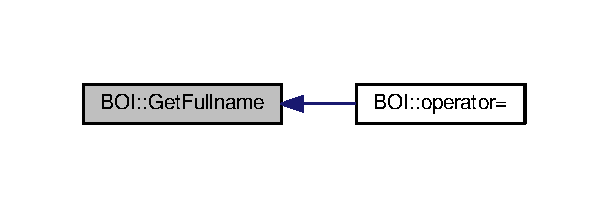
\includegraphics[width=292pt]{class_b_o_i_af56446a377068cd65526e40e8b31b878_icgraph}
\end{center}
\end{figure}


\index{B\+OI@{B\+OI}!Get\+Last\+Name@{Get\+Last\+Name}}
\index{Get\+Last\+Name@{Get\+Last\+Name}!B\+OI@{B\+OI}}
\paragraph[{\texorpdfstring{Get\+Last\+Name() const }{GetLastName() const }}]{\setlength{\rightskip}{0pt plus 5cm}std\+::string B\+O\+I\+::\+Get\+Last\+Name (
\begin{DoxyParamCaption}
{}
\end{DoxyParamCaption}
) const\hspace{0.3cm}{\ttfamily [virtual]}}\hypertarget{class_b_o_i_a37828f3fa4a32f522966e2cad90eaab2}{}\label{class_b_o_i_a37828f3fa4a32f522966e2cad90eaab2}


Implements \hyperlink{class_b_a_n_k_a6588652e6baae302caa39228ecf1606a}{B\+A\+NK}.



Definition at line \hyperlink{_b_o_i_8cpp_source_l00086}{86} of file \hyperlink{_b_o_i_8cpp_source}{B\+O\+I.\+cpp}.



Referenced by \hyperlink{_b_o_i_8h_source_l00065}{operator=()}, and \hyperlink{_b_o_i_8cpp_source_l00054}{to\+String()}.


\begin{DoxyCode}
00086                                  \{
00087     \textcolor{keywordflow}{return} lastName;
00088 \}
\end{DoxyCode}


Here is the caller graph for this function\+:\nopagebreak
\begin{figure}[H]
\begin{center}
\leavevmode
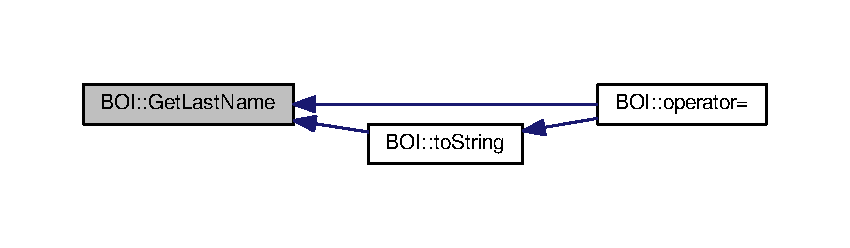
\includegraphics[width=350pt]{class_b_o_i_a37828f3fa4a32f522966e2cad90eaab2_icgraph}
\end{center}
\end{figure}


\index{B\+OI@{B\+OI}!operator=@{operator=}}
\index{operator=@{operator=}!B\+OI@{B\+OI}}
\paragraph[{\texorpdfstring{operator=(const B\+O\+I \&orig)}{operator=(const BOI &orig)}}]{\setlength{\rightskip}{0pt plus 5cm}{\bf B\+OI} B\+O\+I\+::operator= (
\begin{DoxyParamCaption}
\item[{const {\bf B\+OI} \&}]{orig}
\end{DoxyParamCaption}
)\hspace{0.3cm}{\ttfamily [inline]}}\hypertarget{class_b_o_i_a4b4a3976cc13c4d3de0d7ff8882a7af3}{}\label{class_b_o_i_a4b4a3976cc13c4d3de0d7ff8882a7af3}
Operator 

Definition at line \hyperlink{_b_o_i_8h_source_l00065}{65} of file \hyperlink{_b_o_i_8h_source}{B\+O\+I.\+h}.



References \hyperlink{_b_o_i_8cpp_source_l00035}{copy()}, \hyperlink{_b_o_i_8cpp_source_l00078}{Get\+Account\+Number()}, \hyperlink{_b_o_i_8cpp_source_l00062}{Get\+Address()}, \hyperlink{_b_o_i_8cpp_source_l00070}{Get\+Balance()}, \hyperlink{_b_o_i_8cpp_source_l00022}{get\+Base\+Copy()}, \hyperlink{_b_o_i_8cpp_source_l00094}{Get\+First\+Name()}, \hyperlink{_b_o_i_8cpp_source_l00102}{Get\+Fullname()}, \hyperlink{_b_o_i_8cpp_source_l00086}{Get\+Last\+Name()}, \hyperlink{_b_o_i_8cpp_source_l00074}{Set\+Account\+Number()}, \hyperlink{_b_o_i_8cpp_source_l00058}{Set\+Address()}, \hyperlink{_b_o_i_8cpp_source_l00066}{Set\+Balance()}, \hyperlink{_b_o_i_8cpp_source_l00090}{Set\+First\+Name()}, \hyperlink{_b_o_i_8cpp_source_l00098}{Set\+Fullname()}, \hyperlink{_b_o_i_8cpp_source_l00082}{Set\+Last\+Name()}, \hyperlink{_b_o_i_8cpp_source_l00054}{to\+String()}, and \hyperlink{_b_o_i_8cpp_source_l00012}{$\sim$\+B\+O\+I()}.


\begin{DoxyCode}
00065 \{\};
\end{DoxyCode}


Here is the call graph for this function\+:\nopagebreak
\begin{figure}[H]
\begin{center}
\leavevmode
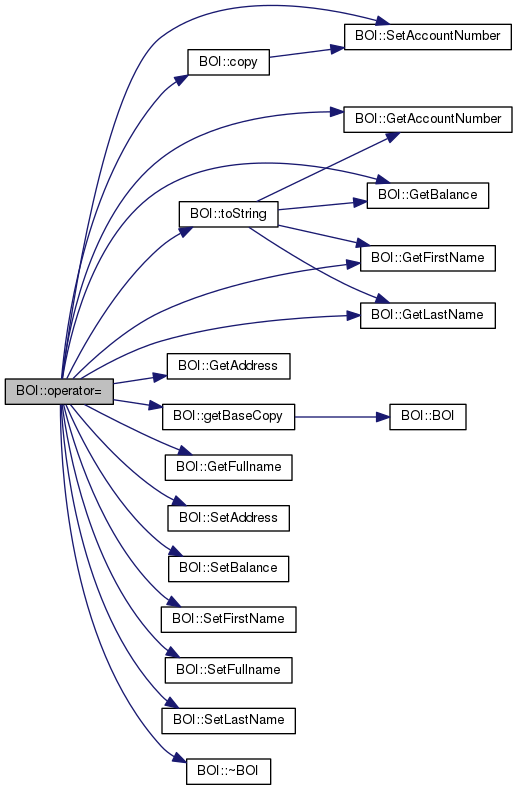
\includegraphics[width=350pt]{class_b_o_i_a4b4a3976cc13c4d3de0d7ff8882a7af3_cgraph}
\end{center}
\end{figure}


\index{B\+OI@{B\+OI}!Set\+Account\+Number@{Set\+Account\+Number}}
\index{Set\+Account\+Number@{Set\+Account\+Number}!B\+OI@{B\+OI}}
\paragraph[{\texorpdfstring{Set\+Account\+Number(int account\+Number)}{SetAccountNumber(int accountNumber)}}]{\setlength{\rightskip}{0pt plus 5cm}void B\+O\+I\+::\+Set\+Account\+Number (
\begin{DoxyParamCaption}
\item[{int}]{account\+Number}
\end{DoxyParamCaption}
)\hspace{0.3cm}{\ttfamily [virtual]}}\hypertarget{class_b_o_i_affc9e7e2a36214b3790f250b7108bb65}{}\label{class_b_o_i_affc9e7e2a36214b3790f250b7108bb65}


Implements \hyperlink{class_b_a_n_k_a1134e7e3d219b7a3aaee42410aa19dfb}{B\+A\+NK}.



Definition at line \hyperlink{_b_o_i_8cpp_source_l00074}{74} of file \hyperlink{_b_o_i_8cpp_source}{B\+O\+I.\+cpp}.



Referenced by \hyperlink{_b_o_i_8cpp_source_l00035}{copy()}, and \hyperlink{_b_o_i_8h_source_l00065}{operator=()}.


\begin{DoxyCode}
00074                                             \{
00075     this->accountNumber = accountNumber;
00076 \}
\end{DoxyCode}


Here is the caller graph for this function\+:\nopagebreak
\begin{figure}[H]
\begin{center}
\leavevmode
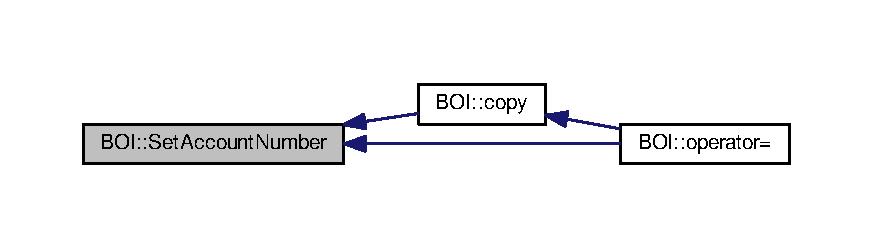
\includegraphics[width=350pt]{class_b_o_i_affc9e7e2a36214b3790f250b7108bb65_icgraph}
\end{center}
\end{figure}


\index{B\+OI@{B\+OI}!Set\+Address@{Set\+Address}}
\index{Set\+Address@{Set\+Address}!B\+OI@{B\+OI}}
\paragraph[{\texorpdfstring{Set\+Address(std\+::string address)}{SetAddress(std::string address)}}]{\setlength{\rightskip}{0pt plus 5cm}void B\+O\+I\+::\+Set\+Address (
\begin{DoxyParamCaption}
\item[{std\+::string}]{address}
\end{DoxyParamCaption}
)\hspace{0.3cm}{\ttfamily [virtual]}}\hypertarget{class_b_o_i_a00c9386c862cf2442968bf7fc30102b3}{}\label{class_b_o_i_a00c9386c862cf2442968bf7fc30102b3}


Implements \hyperlink{class_b_a_n_k_a4044c2f37c8b55b65ed5d57f1867e508}{B\+A\+NK}.



Definition at line \hyperlink{_b_o_i_8cpp_source_l00058}{58} of file \hyperlink{_b_o_i_8cpp_source}{B\+O\+I.\+cpp}.



Referenced by \hyperlink{_b_o_i_8h_source_l00065}{operator=()}.


\begin{DoxyCode}
00058                                       \{
00059     this->address = address;
00060 \}
\end{DoxyCode}


Here is the caller graph for this function\+:\nopagebreak
\begin{figure}[H]
\begin{center}
\leavevmode
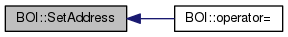
\includegraphics[width=288pt]{class_b_o_i_a00c9386c862cf2442968bf7fc30102b3_icgraph}
\end{center}
\end{figure}


\index{B\+OI@{B\+OI}!Set\+Balance@{Set\+Balance}}
\index{Set\+Balance@{Set\+Balance}!B\+OI@{B\+OI}}
\paragraph[{\texorpdfstring{Set\+Balance(double balance)}{SetBalance(double balance)}}]{\setlength{\rightskip}{0pt plus 5cm}void B\+O\+I\+::\+Set\+Balance (
\begin{DoxyParamCaption}
\item[{double}]{balance}
\end{DoxyParamCaption}
)\hspace{0.3cm}{\ttfamily [virtual]}}\hypertarget{class_b_o_i_a416667693c10f5e4120eec97a9269348}{}\label{class_b_o_i_a416667693c10f5e4120eec97a9269348}


Implements \hyperlink{class_b_a_n_k_a43bef9f486c88a2dc4906eee0e38a394}{B\+A\+NK}.



Definition at line \hyperlink{_b_o_i_8cpp_source_l00066}{66} of file \hyperlink{_b_o_i_8cpp_source}{B\+O\+I.\+cpp}.



Referenced by \hyperlink{_b_o_i_8h_source_l00065}{operator=()}.


\begin{DoxyCode}
00066                                    \{
00067     this->balance = balance;
00068 \}
\end{DoxyCode}


Here is the caller graph for this function\+:\nopagebreak
\begin{figure}[H]
\begin{center}
\leavevmode
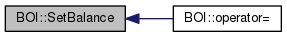
\includegraphics[width=287pt]{class_b_o_i_a416667693c10f5e4120eec97a9269348_icgraph}
\end{center}
\end{figure}


\index{B\+OI@{B\+OI}!Set\+First\+Name@{Set\+First\+Name}}
\index{Set\+First\+Name@{Set\+First\+Name}!B\+OI@{B\+OI}}
\paragraph[{\texorpdfstring{Set\+First\+Name(std\+::string first\+Name)}{SetFirstName(std::string firstName)}}]{\setlength{\rightskip}{0pt plus 5cm}void B\+O\+I\+::\+Set\+First\+Name (
\begin{DoxyParamCaption}
\item[{std\+::string}]{first\+Name}
\end{DoxyParamCaption}
)\hspace{0.3cm}{\ttfamily [virtual]}}\hypertarget{class_b_o_i_ae9042f87be085c2cec799981c30d7d19}{}\label{class_b_o_i_ae9042f87be085c2cec799981c30d7d19}


Implements \hyperlink{class_b_a_n_k_a4baa20e9389c4a592cb0d172c053bf4e}{B\+A\+NK}.



Definition at line \hyperlink{_b_o_i_8cpp_source_l00090}{90} of file \hyperlink{_b_o_i_8cpp_source}{B\+O\+I.\+cpp}.



Referenced by \hyperlink{_b_o_i_8h_source_l00065}{operator=()}.


\begin{DoxyCode}
00090                                           \{
00091     this->firstName = firstName;
00092 \}
\end{DoxyCode}


Here is the caller graph for this function\+:\nopagebreak
\begin{figure}[H]
\begin{center}
\leavevmode
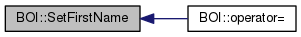
\includegraphics[width=298pt]{class_b_o_i_ae9042f87be085c2cec799981c30d7d19_icgraph}
\end{center}
\end{figure}


\index{B\+OI@{B\+OI}!Set\+Fullname@{Set\+Fullname}}
\index{Set\+Fullname@{Set\+Fullname}!B\+OI@{B\+OI}}
\paragraph[{\texorpdfstring{Set\+Fullname(std\+::string fullname)}{SetFullname(std::string fullname)}}]{\setlength{\rightskip}{0pt plus 5cm}void B\+O\+I\+::\+Set\+Fullname (
\begin{DoxyParamCaption}
\item[{std\+::string}]{fullname}
\end{DoxyParamCaption}
)\hspace{0.3cm}{\ttfamily [virtual]}}\hypertarget{class_b_o_i_a93091f16610f1a1474aea31fd5f81ffd}{}\label{class_b_o_i_a93091f16610f1a1474aea31fd5f81ffd}


Implements \hyperlink{class_b_a_n_k_a02a2f543667403bad41ad614ac9bbde2}{B\+A\+NK}.



Definition at line \hyperlink{_b_o_i_8cpp_source_l00098}{98} of file \hyperlink{_b_o_i_8cpp_source}{B\+O\+I.\+cpp}.



Referenced by \hyperlink{_b_o_i_8h_source_l00065}{operator=()}.


\begin{DoxyCode}
00098                                         \{
00099     this->fullname = fullname;
00100 \}
\end{DoxyCode}


Here is the caller graph for this function\+:\nopagebreak
\begin{figure}[H]
\begin{center}
\leavevmode
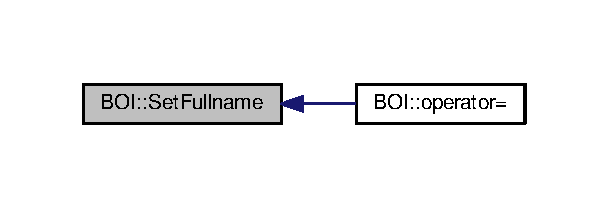
\includegraphics[width=292pt]{class_b_o_i_a93091f16610f1a1474aea31fd5f81ffd_icgraph}
\end{center}
\end{figure}


\index{B\+OI@{B\+OI}!Set\+Last\+Name@{Set\+Last\+Name}}
\index{Set\+Last\+Name@{Set\+Last\+Name}!B\+OI@{B\+OI}}
\paragraph[{\texorpdfstring{Set\+Last\+Name(std\+::string last\+Name)}{SetLastName(std::string lastName)}}]{\setlength{\rightskip}{0pt plus 5cm}void B\+O\+I\+::\+Set\+Last\+Name (
\begin{DoxyParamCaption}
\item[{std\+::string}]{last\+Name}
\end{DoxyParamCaption}
)\hspace{0.3cm}{\ttfamily [virtual]}}\hypertarget{class_b_o_i_a663906e9a59ffa970fb928746c01e8af}{}\label{class_b_o_i_a663906e9a59ffa970fb928746c01e8af}


Implements \hyperlink{class_b_a_n_k_a480fa0973e3e27df92be6767b2f9a652}{B\+A\+NK}.



Definition at line \hyperlink{_b_o_i_8cpp_source_l00082}{82} of file \hyperlink{_b_o_i_8cpp_source}{B\+O\+I.\+cpp}.



Referenced by \hyperlink{_b_o_i_8h_source_l00065}{operator=()}.


\begin{DoxyCode}
00082                                         \{
00083     this->lastName = lastName;
00084 \}
\end{DoxyCode}


Here is the caller graph for this function\+:\nopagebreak
\begin{figure}[H]
\begin{center}
\leavevmode
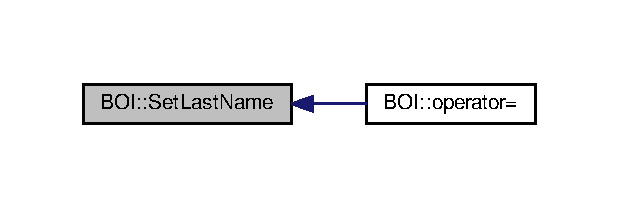
\includegraphics[width=297pt]{class_b_o_i_a663906e9a59ffa970fb928746c01e8af_icgraph}
\end{center}
\end{figure}


\index{B\+OI@{B\+OI}!to\+String@{to\+String}}
\index{to\+String@{to\+String}!B\+OI@{B\+OI}}
\paragraph[{\texorpdfstring{to\+String()}{toString()}}]{\setlength{\rightskip}{0pt plus 5cm}void B\+O\+I\+::to\+String (
\begin{DoxyParamCaption}
{}
\end{DoxyParamCaption}
)\hspace{0.3cm}{\ttfamily [virtual]}}\hypertarget{class_b_o_i_ab02a4dd4ebcc5b2abfaca19f2dff2006}{}\label{class_b_o_i_ab02a4dd4ebcc5b2abfaca19f2dff2006}


\+\_\+cast, is use to cast bak the std\+::shared\+\_\+ptr$<$\+O\+S\+T\+M$>$ to the required type 

to\+String function, displays the object values in formatted way 

Definition at line \hyperlink{_b_o_i_8cpp_source_l00054}{54} of file \hyperlink{_b_o_i_8cpp_source}{B\+O\+I.\+cpp}.



References \hyperlink{_b_o_i_8cpp_source_l00078}{Get\+Account\+Number()}, \hyperlink{_b_o_i_8cpp_source_l00070}{Get\+Balance()}, \hyperlink{_b_o_i_8cpp_source_l00094}{Get\+First\+Name()}, and \hyperlink{_b_o_i_8cpp_source_l00086}{Get\+Last\+Name()}.



Referenced by \hyperlink{_b_o_i_8h_source_l00065}{operator=()}.


\begin{DoxyCode}
00055 \{
00056    std::cout << \textcolor{stringliteral}{"\(\backslash\)nBOI BANK"} << \textcolor{stringliteral}{"\(\backslash\)nUnique ID : "} << this->Get\_Unique\_ID() << \textcolor{stringliteral}{"\(\backslash\)nInt account : "} << this->
      \hyperlink{class_b_o_i_a5b18e1538f3d37835234946cdf9f240f}{GetAccountNumber}() << \textcolor{stringliteral}{"\(\backslash\)nDouble value : "} << this->\hyperlink{class_b_o_i_a25b289dece2a1685bb9d1a9332c9be0b}{GetBalance}() << \textcolor{stringliteral}{"\(\backslash\)nFirst name:
       "} << this->\hyperlink{class_b_o_i_ab4b9d50c6008a666aa4382def580e7d1}{GetFirstName}() << \textcolor{stringliteral}{"\(\backslash\)nLast name : "} << this->\hyperlink{class_b_o_i_a37828f3fa4a32f522966e2cad90eaab2}{GetLastName}()  << \textcolor{stringliteral}{"\(\backslash\)nVersion
       number : "} << this->Get\_Version() << std::endl;
00057 \}
\end{DoxyCode}


Here is the call graph for this function\+:\nopagebreak
\begin{figure}[H]
\begin{center}
\leavevmode
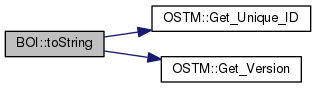
\includegraphics[width=316pt]{class_b_o_i_ab02a4dd4ebcc5b2abfaca19f2dff2006_cgraph}
\end{center}
\end{figure}




Here is the caller graph for this function\+:\nopagebreak
\begin{figure}[H]
\begin{center}
\leavevmode
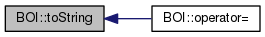
\includegraphics[width=271pt]{class_b_o_i_ab02a4dd4ebcc5b2abfaca19f2dff2006_icgraph}
\end{center}
\end{figure}




The documentation for this class was generated from the following files\+:\begin{DoxyCompactItemize}
\item 
\hyperlink{_b_o_i_8h}{B\+O\+I.\+h}\item 
\hyperlink{_b_o_i_8cpp}{B\+O\+I.\+cpp}\end{DoxyCompactItemize}

\hypertarget{classclient}{}\subsection{client Class Reference}
\label{classclient}\index{client@{client}}


{\ttfamily \#include $<$client.\+h$>$}



Collaboration diagram for client\+:
\nopagebreak
\begin{figure}[H]
\begin{center}
\leavevmode
\includegraphics[width=216pt]{classclient__coll__graph}
\end{center}
\end{figure}
\subsubsection*{Public Member Functions}
\begin{DoxyCompactItemize}
\item 
void \hyperlink{classclient_a3c5e378b6df49d2d2eea4a073da5a594_a3c5e378b6df49d2d2eea4a073da5a594}{\+\_\+complex\+\_\+transfer\+\_\+} (std\+::shared\+\_\+ptr$<$ \hyperlink{class_o_s_t_m}{O\+S\+TM} $>$ \+\_\+from\+\_\+, std\+::shared\+\_\+ptr$<$ \hyperlink{class_o_s_t_m}{O\+S\+TM} $>$ \+\_\+from\+\_\+two\+\_\+, std\+::vector$<$ std\+::shared\+\_\+ptr$<$ \hyperlink{class_o_s_t_m}{O\+S\+TM} $>$$>$ \+\_\+customer\+\_\+vec, \hyperlink{class_t_m}{TM} \&\+\_\+tm, double \+\_\+amount)
\item 
void \hyperlink{classclient_ac0ebebd379895869c22f8919ad3bd37f_ac0ebebd379895869c22f8919ad3bd37f}{\+\_\+nesting\+\_\+} (std\+::shared\+\_\+ptr$<$ \hyperlink{class_o_s_t_m}{O\+S\+TM} $>$ \+\_\+to\+\_\+, std\+::shared\+\_\+ptr$<$ \hyperlink{class_o_s_t_m}{O\+S\+TM} $>$ \+\_\+from\+\_\+, \hyperlink{class_t_m}{TM} \&tm, double \+\_\+amount)
\item 
void \hyperlink{classclient_a94fb0b42124860568a011ed94f8bc9d5_a94fb0b42124860568a011ed94f8bc9d5}{\+\_\+six\+\_\+account\+\_\+transfer\+\_\+} (std\+::shared\+\_\+ptr$<$ \hyperlink{class_o_s_t_m}{O\+S\+TM} $>$ \+\_\+to\+\_\+, std\+::shared\+\_\+ptr$<$ \hyperlink{class_o_s_t_m}{O\+S\+TM} $>$ \+\_\+from\+\_\+one\+\_\+, std\+::shared\+\_\+ptr$<$ \hyperlink{class_o_s_t_m}{O\+S\+TM} $>$ \+\_\+from\+\_\+two\+\_\+, std\+::shared\+\_\+ptr$<$ \hyperlink{class_o_s_t_m}{O\+S\+TM} $>$ \+\_\+from\+\_\+three\+\_\+, std\+::shared\+\_\+ptr$<$ \hyperlink{class_o_s_t_m}{O\+S\+TM} $>$ \+\_\+from\+\_\+four\+\_\+, std\+::shared\+\_\+ptr$<$ \hyperlink{class_o_s_t_m}{O\+S\+TM} $>$ \+\_\+from\+\_\+five\+\_\+, \hyperlink{class_t_m}{TM} \&\+\_\+tm, double \+\_\+amount)
\item 
void \hyperlink{classclient_a71edd1265ba9ae03f71b5dbf54548696_a71edd1265ba9ae03f71b5dbf54548696}{\+\_\+two\+\_\+account\+\_\+transfer\+\_\+} (std\+::shared\+\_\+ptr$<$ \hyperlink{class_o_s_t_m}{O\+S\+TM} $>$ \+\_\+to\+\_\+, std\+::shared\+\_\+ptr$<$ \hyperlink{class_o_s_t_m}{O\+S\+TM} $>$ \+\_\+from\+\_\+, \hyperlink{class_t_m}{TM} \&tm, double \+\_\+amount)
\item 
\hyperlink{classclient_a62e0309db8390260d05d8c3084c6fdd4_a62e0309db8390260d05d8c3084c6fdd4}{client} (int \hyperlink{classclient_a30e2070077d9ba875bfa6616a43d879c_a30e2070077d9ba875bfa6616a43d879c}{value})
\end{DoxyCompactItemize}
\subsubsection*{Public Attributes}
\begin{DoxyCompactItemize}
\item 
int \hyperlink{classclient_a30e2070077d9ba875bfa6616a43d879c_a30e2070077d9ba875bfa6616a43d879c}{value} = 0
\end{DoxyCompactItemize}


\subsubsection{Detailed Description}


Definition at line \hyperlink{client_8h_source_l00034}{34} of file \hyperlink{client_8h_source}{client.\+h}.



\subsubsection{Constructor \& Destructor Documentation}
\index{client@{client}!client@{client}}
\index{client@{client}!client@{client}}
\paragraph[{\texorpdfstring{client(int value)}{client(int value)}}]{\setlength{\rightskip}{0pt plus 5cm}client\+::client (
\begin{DoxyParamCaption}
\item[{int}]{value}
\end{DoxyParamCaption}
)\hspace{0.3cm}{\ttfamily [inline]}}\hypertarget{classclient_a62e0309db8390260d05d8c3084c6fdd4_a62e0309db8390260d05d8c3084c6fdd4}{}\label{classclient_a62e0309db8390260d05d8c3084c6fdd4_a62e0309db8390260d05d8c3084c6fdd4}


Definition at line \hyperlink{client_8h_source_l00039}{39} of file \hyperlink{client_8h_source}{client.\+h}.



References \hyperlink{client_8h_source_l00038}{value}.


\begin{DoxyCode}
00039 \{ this->\hyperlink{classclient_a30e2070077d9ba875bfa6616a43d879c_a30e2070077d9ba875bfa6616a43d879c}{value} = \hyperlink{classclient_a30e2070077d9ba875bfa6616a43d879c_a30e2070077d9ba875bfa6616a43d879c}{value}; \};
\end{DoxyCode}


\subsubsection{Member Function Documentation}
\index{client@{client}!\+\_\+complex\+\_\+transfer\+\_\+@{\+\_\+complex\+\_\+transfer\+\_\+}}
\index{\+\_\+complex\+\_\+transfer\+\_\+@{\+\_\+complex\+\_\+transfer\+\_\+}!client@{client}}
\paragraph[{\texorpdfstring{\+\_\+complex\+\_\+transfer\+\_\+(std\+::shared\+\_\+ptr$<$ O\+S\+T\+M $>$ \+\_\+from\+\_\+, std\+::shared\+\_\+ptr$<$ O\+S\+T\+M $>$ \+\_\+from\+\_\+two\+\_\+, std\+::vector$<$ std\+::shared\+\_\+ptr$<$ O\+S\+T\+M $>$$>$ \+\_\+customer\+\_\+vec, T\+M \&\+\_\+tm, double \+\_\+amount)}{_complex_transfer_(std::shared_ptr< OSTM > _from_, std::shared_ptr< OSTM > _from_two_, std::vector< std::shared_ptr< OSTM >> _customer_vec, TM &_tm, double _amount)}}]{\setlength{\rightskip}{0pt plus 5cm}void client\+::\+\_\+complex\+\_\+transfer\+\_\+ (
\begin{DoxyParamCaption}
\item[{std\+::shared\+\_\+ptr$<$ {\bf O\+S\+TM} $>$}]{\+\_\+from\+\_\+, }
\item[{std\+::shared\+\_\+ptr$<$ {\bf O\+S\+TM} $>$}]{\+\_\+from\+\_\+two\+\_\+, }
\item[{std\+::vector$<$ std\+::shared\+\_\+ptr$<$ {\bf O\+S\+TM} $>$$>$}]{\+\_\+customer\+\_\+vec, }
\item[{{\bf TM} \&}]{\+\_\+tm, }
\item[{double}]{\+\_\+amount}
\end{DoxyParamCaption}
)\hspace{0.3cm}{\ttfamily [inline]}}\hypertarget{classclient_a3c5e378b6df49d2d2eea4a073da5a594_a3c5e378b6df49d2d2eea4a073da5a594}{}\label{classclient_a3c5e378b6df49d2d2eea4a073da5a594_a3c5e378b6df49d2d2eea4a073da5a594}


Definition at line \hyperlink{client_8h_source_l00236}{236} of file \hyperlink{client_8h_source}{client.\+h}.



References \hyperlink{_t_m_8cpp_source_l00079}{T\+M\+::\+\_\+get\+\_\+tx()}, and \hyperlink{_b_a_n_k_8h_source_l00046}{B\+A\+N\+K\+::\+Set\+Balance()}.


\begin{DoxyCode}
00236                                                                                                            
                                                      \{
00237     std::shared\_ptr<TX> tx = \_tm.\hyperlink{class_t_m_a41cb0226cc4080c931651b13f74a0075_a41cb0226cc4080c931651b13f74a0075}{\_get\_tx}();
00238     \textcolor{comment}{/* Register the two single account*/}
00239     tx->\_register(\_from\_);
00240     tx->\_register(\_from\_two\_);
00241     \textcolor{comment}{/* Declare required pointers */}
00242     std::shared\_ptr<OSTM> \_FROM\_OSTM\_ONE\_, \_FROM\_OSTM\_TWO\_, \_TO\_OSTM\_;
00243     std::shared\_ptr<BANK> \_FROM\_, \_FROM\_TWO\_, \_TO\_;
00244 
00245     \textcolor{keywordtype}{bool} done = \textcolor{keyword}{false};
00246     \textcolor{keywordflow}{try} \{
00247         \textcolor{keywordflow}{while} (!done) \{
00248             \textcolor{keywordflow}{for} (\textcolor{keyword}{auto}&& obj : \_customer\_vec) \{
00249                 \textcolor{comment}{/* Register customers accounts from the collection (vector) */}
00250                 tx->\_register(obj);
00251                 \textcolor{comment}{/* From std::shared\_ptr<OSTM> to std::shared\_ptr<BANK> to access the virtual methods  */}
00252                 \_FROM\_ = std::dynamic\_pointer\_cast<\hyperlink{class_b_a_n_k}{BANK}> (tx->load(\_from\_));
00253                 \_FROM\_TWO\_ = std::dynamic\_pointer\_cast<\hyperlink{class_b_a_n_k}{BANK}> (tx->load(\_from\_two\_));
00254                 \_TO\_ = std::dynamic\_pointer\_cast<\hyperlink{class_b_a_n_k}{BANK}> (tx->load(obj));
00255                 \textcolor{comment}{/* Make changes with the objects */}
00256                 \_FROM\_->\hyperlink{class_b_a_n_k_ae3e45b407bf8ec7175662442ea24b7c0_ae3e45b407bf8ec7175662442ea24b7c0}{SetBalance}(\_FROM\_->GetBalance() - \_amount);
00257                 \_FROM\_TWO\_->SetBalance(\_FROM\_TWO\_->GetBalance() - \_amount);
00258                 \_TO\_->SetBalance(\_TO\_->GetBalance() + (\_amount * 2));
00259                 \textcolor{comment}{/* From std::shared\_ptr<BANK> to std::shared\_ptr<OSTM> to store the memory spaces */}
00260                 \_FROM\_OSTM\_ONE\_ = std::dynamic\_pointer\_cast<\hyperlink{class_o_s_t_m}{OSTM}> (\_FROM\_);
00261                 \_FROM\_OSTM\_TWO\_ = std::dynamic\_pointer\_cast<\hyperlink{class_o_s_t_m}{OSTM}> (\_FROM\_TWO\_);
00262                 \_TO\_OSTM\_ = std::dynamic\_pointer\_cast<\hyperlink{class_o_s_t_m}{OSTM}> (\_TO\_);
00263                 \textcolor{comment}{/* Store changes */}
00264                 tx->store(\_FROM\_OSTM\_ONE\_);
00265                 tx->store(\_FROM\_OSTM\_TWO\_);
00266                 tx->store(\_TO\_OSTM\_);
00267             \}
00268             \textcolor{comment}{/* Commit changes */}
00269             done = tx->commit();
00270         \}
00271     \} \textcolor{keywordflow}{catch} (std::runtime\_error& e) \{
00272         std::cout << e.what() << std::endl;
00273     \}
00274 \}
\end{DoxyCode}


Here is the call graph for this function\+:
\nopagebreak
\begin{figure}[H]
\begin{center}
\leavevmode
\includegraphics[width=350pt]{classclient_a3c5e378b6df49d2d2eea4a073da5a594_a3c5e378b6df49d2d2eea4a073da5a594_cgraph}
\end{center}
\end{figure}


\index{client@{client}!\+\_\+nesting\+\_\+@{\+\_\+nesting\+\_\+}}
\index{\+\_\+nesting\+\_\+@{\+\_\+nesting\+\_\+}!client@{client}}
\paragraph[{\texorpdfstring{\+\_\+nesting\+\_\+(std\+::shared\+\_\+ptr$<$ O\+S\+T\+M $>$ \+\_\+to\+\_\+, std\+::shared\+\_\+ptr$<$ O\+S\+T\+M $>$ \+\_\+from\+\_\+, T\+M \&tm, double \+\_\+amount)}{_nesting_(std::shared_ptr< OSTM > _to_, std::shared_ptr< OSTM > _from_, TM &tm, double _amount)}}]{\setlength{\rightskip}{0pt plus 5cm}void client\+::\+\_\+nesting\+\_\+ (
\begin{DoxyParamCaption}
\item[{std\+::shared\+\_\+ptr$<$ {\bf O\+S\+TM} $>$}]{\+\_\+to\+\_\+, }
\item[{std\+::shared\+\_\+ptr$<$ {\bf O\+S\+TM} $>$}]{\+\_\+from\+\_\+, }
\item[{{\bf TM} \&}]{tm, }
\item[{double}]{\+\_\+amount}
\end{DoxyParamCaption}
)\hspace{0.3cm}{\ttfamily [inline]}}\hypertarget{classclient_ac0ebebd379895869c22f8919ad3bd37f_ac0ebebd379895869c22f8919ad3bd37f}{}\label{classclient_ac0ebebd379895869c22f8919ad3bd37f_ac0ebebd379895869c22f8919ad3bd37f}


Definition at line \hyperlink{client_8h_source_l00089}{89} of file \hyperlink{client_8h_source}{client.\+h}.



References \hyperlink{_t_m_8cpp_source_l00079}{T\+M\+::\+\_\+get\+\_\+tx()}, \hyperlink{client_8h_source_l00041}{\+\_\+two\+\_\+account\+\_\+transfer\+\_\+()}, and \hyperlink{_b_a_n_k_8h_source_l00046}{B\+A\+N\+K\+::\+Set\+Balance()}.



Referenced by \hyperlink{_my_test_c_ase_8cpp_source_l00787}{My\+Test\+C\+Ase\+::nested\+\_\+transaction\+\_\+object\+\_\+test()}.


\begin{DoxyCode}
00089                                                                                              \{
00090     std::shared\_ptr<TX> tx = tm.\hyperlink{class_t_m_a41cb0226cc4080c931651b13f74a0075_a41cb0226cc4080c931651b13f74a0075}{\_get\_tx}();
00091     \textcolor{comment}{/*}
00092 \textcolor{comment}{     * Register the two single account}
00093 \textcolor{comment}{     */}
00094     tx->\_register(\_to\_);
00095     tx->\_register(\_from\_);
00096     \textcolor{comment}{/*}
00097 \textcolor{comment}{     * Declare required pointers }
00098 \textcolor{comment}{     */}
00099     std::shared\_ptr<BANK> \_TO\_BANK\_, \_FROM\_BANK\_;
00100     std::shared\_ptr<OSTM> \_TO\_OSTM\_, \_FROM\_OSTM\_;
00101 
00102 
00103     \textcolor{keywordtype}{bool} done = \textcolor{keyword}{false};
00104     \textcolor{keywordflow}{try} \{
00105         \textcolor{keywordflow}{while} (!done) \{
00106             \textcolor{comment}{/*}
00107 \textcolor{comment}{             * From std::shared\_ptr<OSTM> to std::shared\_ptr<BANK> to access the virtual methods}
00108 \textcolor{comment}{             */}
00109             \_TO\_BANK\_ = std::dynamic\_pointer\_cast<\hyperlink{class_b_a_n_k}{BANK}> (tx->load(\_to\_));
00110             \_FROM\_BANK\_ = std::dynamic\_pointer\_cast<\hyperlink{class_b_a_n_k}{BANK}> (tx->load(\_from\_));
00111             \textcolor{comment}{/*}
00112 \textcolor{comment}{             * Make changes with the objects}
00113 \textcolor{comment}{             */}
00114             \_TO\_BANK\_->\hyperlink{class_b_a_n_k_ae3e45b407bf8ec7175662442ea24b7c0_ae3e45b407bf8ec7175662442ea24b7c0}{SetBalance}(\_TO\_BANK\_->GetBalance() + \_amount);
00115             \_FROM\_BANK\_->SetBalance(\_FROM\_BANK\_->GetBalance() - \_amount);
00116             \textcolor{comment}{/*}
00117 \textcolor{comment}{             * From std::shared\_ptr<BANK> to std::shared\_ptr<OSTM> to store the memory spaces}
00118 \textcolor{comment}{             */}
00119             \_TO\_OSTM\_ = std::dynamic\_pointer\_cast<\hyperlink{class_o_s_t_m}{OSTM}> (\_TO\_BANK\_);
00120             \_FROM\_OSTM\_ = std::dynamic\_pointer\_cast<\hyperlink{class_o_s_t_m}{OSTM}> (\_FROM\_BANK\_);
00121             \textcolor{comment}{/*}
00122 \textcolor{comment}{             * Store changes}
00123 \textcolor{comment}{             */}
00124             tx->store(\_TO\_OSTM\_);
00125             tx->store(\_FROM\_OSTM\_);
00126 
00127             \textcolor{comment}{/*}
00128 \textcolor{comment}{             * NESTED TRANSACTION}
00129 \textcolor{comment}{             */}
00130             std::shared\_ptr<TX> txTwo = tm.\hyperlink{class_t_m_a41cb0226cc4080c931651b13f74a0075_a41cb0226cc4080c931651b13f74a0075}{\_get\_tx}();
00131 
00132             \textcolor{keywordtype}{bool} nestedDone = \textcolor{keyword}{false};
00133             \textcolor{keywordflow}{while} (!nestedDone) \{
00134                 \_TO\_BANK\_ = std::dynamic\_pointer\_cast<\hyperlink{class_b_a_n_k}{BANK}> (txTwo->load(\_to\_));
00135                 \_FROM\_BANK\_ = std::dynamic\_pointer\_cast<\hyperlink{class_b_a_n_k}{BANK}> (txTwo->load(\_from\_));
00136                 \textcolor{comment}{/*}
00137 \textcolor{comment}{                 * Make changes with the objects}
00138 \textcolor{comment}{                 */}
00139                 \_TO\_BANK\_->\hyperlink{class_b_a_n_k_ae3e45b407bf8ec7175662442ea24b7c0_ae3e45b407bf8ec7175662442ea24b7c0}{SetBalance}(\_TO\_BANK\_->GetBalance() + \_amount);
00140                 \_FROM\_BANK\_->SetBalance(\_FROM\_BANK\_->GetBalance() - \_amount);
00141                 \textcolor{comment}{/*}
00142 \textcolor{comment}{                 * From std::shared\_ptr<BANK> to std::shared\_ptr<OSTM> to store the memory spaces}
00143 \textcolor{comment}{                 */}
00144                 \_TO\_OSTM\_ = std::dynamic\_pointer\_cast<\hyperlink{class_o_s_t_m}{OSTM}> (\_TO\_BANK\_);
00145                 \_FROM\_OSTM\_ = std::dynamic\_pointer\_cast<\hyperlink{class_o_s_t_m}{OSTM}> (\_FROM\_BANK\_);
00146                 \textcolor{comment}{/*}
00147 \textcolor{comment}{                 * Store changes}
00148 \textcolor{comment}{                 */}
00149                 txTwo->store(\_TO\_OSTM\_);
00150                 txTwo->store(\_FROM\_OSTM\_);
00151                 \textcolor{comment}{/*}
00152 \textcolor{comment}{                 * NESTED TRANSACTION IN THE NESTED TRANSACTION}
00153 \textcolor{comment}{                 * \_two\_account\_transfer\_ function call}
00154 \textcolor{comment}{                 */}
00155                 \hyperlink{classclient_a71edd1265ba9ae03f71b5dbf54548696_a71edd1265ba9ae03f71b5dbf54548696}{\_two\_account\_transfer\_}(\_to\_, \_from\_, tm, \_amount);
00156 
00157                 nestedDone = txTwo->commit();
00158             \}
00159 
00160             \textcolor{comment}{/*}
00161 \textcolor{comment}{             * Commit changes}
00162 \textcolor{comment}{             */}
00163             done = tx->commit();
00164         \}
00165     \} \textcolor{keywordflow}{catch} (std::runtime\_error& e) \{
00166         std::cout << e.what() << std::endl;
00167     \}
00168 \}
\end{DoxyCode}


Here is the call graph for this function\+:
\nopagebreak
\begin{figure}[H]
\begin{center}
\leavevmode
\includegraphics[width=350pt]{classclient_ac0ebebd379895869c22f8919ad3bd37f_ac0ebebd379895869c22f8919ad3bd37f_cgraph}
\end{center}
\end{figure}


\index{client@{client}!\+\_\+six\+\_\+account\+\_\+transfer\+\_\+@{\+\_\+six\+\_\+account\+\_\+transfer\+\_\+}}
\index{\+\_\+six\+\_\+account\+\_\+transfer\+\_\+@{\+\_\+six\+\_\+account\+\_\+transfer\+\_\+}!client@{client}}
\paragraph[{\texorpdfstring{\+\_\+six\+\_\+account\+\_\+transfer\+\_\+(std\+::shared\+\_\+ptr$<$ O\+S\+T\+M $>$ \+\_\+to\+\_\+, std\+::shared\+\_\+ptr$<$ O\+S\+T\+M $>$ \+\_\+from\+\_\+one\+\_\+, std\+::shared\+\_\+ptr$<$ O\+S\+T\+M $>$ \+\_\+from\+\_\+two\+\_\+, std\+::shared\+\_\+ptr$<$ O\+S\+T\+M $>$ \+\_\+from\+\_\+three\+\_\+, std\+::shared\+\_\+ptr$<$ O\+S\+T\+M $>$ \+\_\+from\+\_\+four\+\_\+, std\+::shared\+\_\+ptr$<$ O\+S\+T\+M $>$ \+\_\+from\+\_\+five\+\_\+, T\+M \&\+\_\+tm, double \+\_\+amount)}{_six_account_transfer_(std::shared_ptr< OSTM > _to_, std::shared_ptr< OSTM > _from_one_, std::shared_ptr< OSTM > _from_two_, std::shared_ptr< OSTM > _from_three_, std::shared_ptr< OSTM > _from_four_, std::shared_ptr< OSTM > _from_five_, TM &_tm, double _amount)}}]{\setlength{\rightskip}{0pt plus 5cm}void client\+::\+\_\+six\+\_\+account\+\_\+transfer\+\_\+ (
\begin{DoxyParamCaption}
\item[{std\+::shared\+\_\+ptr$<$ {\bf O\+S\+TM} $>$}]{\+\_\+to\+\_\+, }
\item[{std\+::shared\+\_\+ptr$<$ {\bf O\+S\+TM} $>$}]{\+\_\+from\+\_\+one\+\_\+, }
\item[{std\+::shared\+\_\+ptr$<$ {\bf O\+S\+TM} $>$}]{\+\_\+from\+\_\+two\+\_\+, }
\item[{std\+::shared\+\_\+ptr$<$ {\bf O\+S\+TM} $>$}]{\+\_\+from\+\_\+three\+\_\+, }
\item[{std\+::shared\+\_\+ptr$<$ {\bf O\+S\+TM} $>$}]{\+\_\+from\+\_\+four\+\_\+, }
\item[{std\+::shared\+\_\+ptr$<$ {\bf O\+S\+TM} $>$}]{\+\_\+from\+\_\+five\+\_\+, }
\item[{{\bf TM} \&}]{\+\_\+tm, }
\item[{double}]{\+\_\+amount}
\end{DoxyParamCaption}
)\hspace{0.3cm}{\ttfamily [inline]}}\hypertarget{classclient_a94fb0b42124860568a011ed94f8bc9d5_a94fb0b42124860568a011ed94f8bc9d5}{}\label{classclient_a94fb0b42124860568a011ed94f8bc9d5_a94fb0b42124860568a011ed94f8bc9d5}


Definition at line \hyperlink{client_8h_source_l00170}{170} of file \hyperlink{client_8h_source}{client.\+h}.



References \hyperlink{_t_m_8cpp_source_l00079}{T\+M\+::\+\_\+get\+\_\+tx()}, and \hyperlink{_b_a_n_k_8h_source_l00046}{B\+A\+N\+K\+::\+Set\+Balance()}.


\begin{DoxyCode}
00170                                                                                                            
                                                                                                                  
                                  \{
00171     std::shared\_ptr<TX> tx = \_tm.\hyperlink{class_t_m_a41cb0226cc4080c931651b13f74a0075_a41cb0226cc4080c931651b13f74a0075}{\_get\_tx}();
00172     \textcolor{comment}{/*}
00173 \textcolor{comment}{     * Register the two single account}
00174 \textcolor{comment}{     */}
00175     tx->\_register(\_to\_);
00176     tx->\_register(\_from\_one\_);
00177     tx->\_register(\_from\_two\_);
00178     tx->\_register(\_from\_three\_);
00179     tx->\_register(\_from\_four\_);
00180     tx->\_register(\_from\_five\_);
00181 
00182     \textcolor{comment}{/*}
00183 \textcolor{comment}{     * Required pointers to use in transaction}
00184 \textcolor{comment}{     */}
00185     std::shared\_ptr<OSTM> \_TO\_OSTM, \_FROM\_ONE\_OSTM, \_FROM\_TWO\_OSTM, \_FROM\_THREE\_OSTM, \_FROM\_FOUR\_OSTM, 
      \_FROM\_FIVE\_OSTM;
00186     std::shared\_ptr<BANK> \_TO\_, \_FROM\_ONE\_, \_FROM\_TWO\_, \_FROM\_THREE\_, \_FROM\_FOUR\_, \_FROM\_FIVE\_;
00187     \textcolor{keywordflow}{try} \{
00188         \textcolor{keywordtype}{bool} done = \textcolor{keyword}{false};
00189         \textcolor{keywordflow}{while} (!done) \{
00190             \textcolor{comment}{/*}
00191 \textcolor{comment}{             * From std::shared\_ptr<OSTM> to std::shared\_ptr<BANK> to access the virtual methods}
00192 \textcolor{comment}{             */}
00193             \_TO\_ = std::dynamic\_pointer\_cast<\hyperlink{class_b_a_n_k}{BANK}> (tx->load(\_to\_));
00194             \_FROM\_ONE\_ = std::dynamic\_pointer\_cast<\hyperlink{class_b_a_n_k}{BANK}> (tx->load(\_from\_one\_));
00195             \_FROM\_TWO\_ = std::dynamic\_pointer\_cast<\hyperlink{class_b_a_n_k}{BANK}> (tx->load(\_from\_two\_));
00196             \_FROM\_THREE\_ = std::dynamic\_pointer\_cast<\hyperlink{class_b_a_n_k}{BANK}> (tx->load(\_from\_three\_));
00197             \_FROM\_FOUR\_ = std::dynamic\_pointer\_cast<\hyperlink{class_b_a_n_k}{BANK}> (tx->load(\_from\_four\_));
00198             \_FROM\_FIVE\_ = std::dynamic\_pointer\_cast<\hyperlink{class_b_a_n_k}{BANK}> (tx->load(\_from\_five\_));
00199             \textcolor{comment}{/*}
00200 \textcolor{comment}{             * Make changes with the objects}
00201 \textcolor{comment}{             */}
00202             \_TO\_->\hyperlink{class_b_a_n_k_ae3e45b407bf8ec7175662442ea24b7c0_ae3e45b407bf8ec7175662442ea24b7c0}{SetBalance}(\_TO\_->GetBalance() + (\_amount * 5));
00203             \_FROM\_ONE\_->SetBalance(\_FROM\_ONE\_->GetBalance() - \_amount);
00204             \_FROM\_TWO\_->SetBalance(\_FROM\_TWO\_->GetBalance() - \_amount);
00205             \_FROM\_THREE\_->SetBalance(\_FROM\_THREE\_->GetBalance() - \_amount);
00206             \_FROM\_FOUR\_->SetBalance(\_FROM\_FOUR\_->GetBalance() - \_amount);
00207             \_FROM\_FIVE\_->SetBalance(\_FROM\_FIVE\_->GetBalance() - \_amount);
00208             \textcolor{comment}{/*}
00209 \textcolor{comment}{             * From std::shared\_ptr<BANK> to std::shared\_ptr<OSTM> to store the memory spaces}
00210 \textcolor{comment}{             */}
00211             \_TO\_OSTM = std::dynamic\_pointer\_cast<\hyperlink{class_o_s_t_m}{OSTM}> (\_TO\_);
00212             \_FROM\_ONE\_OSTM = std::dynamic\_pointer\_cast<\hyperlink{class_o_s_t_m}{OSTM}> (\_FROM\_ONE\_);
00213             \_FROM\_TWO\_OSTM = std::dynamic\_pointer\_cast<\hyperlink{class_o_s_t_m}{OSTM}> (\_FROM\_TWO\_);
00214             \_FROM\_THREE\_OSTM = std::dynamic\_pointer\_cast<\hyperlink{class_o_s_t_m}{OSTM}> (\_FROM\_THREE\_);
00215             \_FROM\_FOUR\_OSTM = std::dynamic\_pointer\_cast<\hyperlink{class_o_s_t_m}{OSTM}> (\_FROM\_FOUR\_);
00216             \_FROM\_FIVE\_OSTM = std::dynamic\_pointer\_cast<\hyperlink{class_o_s_t_m}{OSTM}> (\_FROM\_FIVE\_);
00217             \textcolor{comment}{/*}
00218 \textcolor{comment}{             * Store changes}
00219 \textcolor{comment}{             */}
00220             tx->store(\_TO\_OSTM);
00221             tx->store(\_FROM\_ONE\_OSTM);
00222             tx->store(\_FROM\_TWO\_OSTM);
00223             tx->store(\_FROM\_THREE\_OSTM);
00224             tx->store(\_FROM\_FOUR\_OSTM);
00225             tx->store(\_FROM\_FIVE\_OSTM);
00226             \textcolor{comment}{/*}
00227 \textcolor{comment}{             * Commit changes}
00228 \textcolor{comment}{             */}
00229             done = tx->commit();
00230         \}
00231     \} \textcolor{keywordflow}{catch} (std::runtime\_error& e) \{
00232         std::cout << e.what() << std::endl;
00233     \}
00234 \}
\end{DoxyCode}


Here is the call graph for this function\+:
\nopagebreak
\begin{figure}[H]
\begin{center}
\leavevmode
\includegraphics[width=350pt]{classclient_a94fb0b42124860568a011ed94f8bc9d5_a94fb0b42124860568a011ed94f8bc9d5_cgraph}
\end{center}
\end{figure}


\index{client@{client}!\+\_\+two\+\_\+account\+\_\+transfer\+\_\+@{\+\_\+two\+\_\+account\+\_\+transfer\+\_\+}}
\index{\+\_\+two\+\_\+account\+\_\+transfer\+\_\+@{\+\_\+two\+\_\+account\+\_\+transfer\+\_\+}!client@{client}}
\paragraph[{\texorpdfstring{\+\_\+two\+\_\+account\+\_\+transfer\+\_\+(std\+::shared\+\_\+ptr$<$ O\+S\+T\+M $>$ \+\_\+to\+\_\+, std\+::shared\+\_\+ptr$<$ O\+S\+T\+M $>$ \+\_\+from\+\_\+, T\+M \&tm, double \+\_\+amount)}{_two_account_transfer_(std::shared_ptr< OSTM > _to_, std::shared_ptr< OSTM > _from_, TM &tm, double _amount)}}]{\setlength{\rightskip}{0pt plus 5cm}void client\+::\+\_\+two\+\_\+account\+\_\+transfer\+\_\+ (
\begin{DoxyParamCaption}
\item[{std\+::shared\+\_\+ptr$<$ {\bf O\+S\+TM} $>$}]{\+\_\+to\+\_\+, }
\item[{std\+::shared\+\_\+ptr$<$ {\bf O\+S\+TM} $>$}]{\+\_\+from\+\_\+, }
\item[{{\bf TM} \&}]{tm, }
\item[{double}]{\+\_\+amount}
\end{DoxyParamCaption}
)\hspace{0.3cm}{\ttfamily [inline]}}\hypertarget{classclient_a71edd1265ba9ae03f71b5dbf54548696_a71edd1265ba9ae03f71b5dbf54548696}{}\label{classclient_a71edd1265ba9ae03f71b5dbf54548696_a71edd1265ba9ae03f71b5dbf54548696}


Definition at line \hyperlink{client_8h_source_l00041}{41} of file \hyperlink{client_8h_source}{client.\+h}.



References \hyperlink{_t_m_8cpp_source_l00079}{T\+M\+::\+\_\+get\+\_\+tx()}, and \hyperlink{_b_a_n_k_8h_source_l00046}{B\+A\+N\+K\+::\+Set\+Balance()}.



Referenced by \hyperlink{client_8h_source_l00089}{\+\_\+nesting\+\_\+()}, \hyperlink{_my_test_c_ase_8cpp_source_l00748}{My\+Test\+C\+Ase\+::two\+\_\+object\+\_\+transfer\+\_\+complete()}, and \hyperlink{_my_test_c_ase_8cpp_source_l00765}{My\+Test\+C\+Ase\+::two\+\_\+object\+\_\+transfer\+\_\+state\+\_\+change()}.


\begin{DoxyCode}
00041                                                                                                            
         \{
00042 
00043     std::shared\_ptr<TX> tx = tm.\hyperlink{class_t_m_a41cb0226cc4080c931651b13f74a0075_a41cb0226cc4080c931651b13f74a0075}{\_get\_tx}();
00044     \textcolor{comment}{/*}
00045 \textcolor{comment}{     * Register the two single account}
00046 \textcolor{comment}{     */}
00047     tx->\_register(\_to\_);
00048     tx->\_register(\_from\_);
00049     \textcolor{comment}{/*}
00050 \textcolor{comment}{     * Declare required pointers }
00051 \textcolor{comment}{     */}
00052     std::shared\_ptr<BANK> \_TO\_BANK\_, \_FROM\_BANK\_;
00053     std::shared\_ptr<OSTM> \_TO\_OSTM\_, \_FROM\_OSTM\_;
00054 
00055     \textcolor{keywordtype}{bool} done = \textcolor{keyword}{false};
00056     \textcolor{keywordflow}{try} \{
00057         \textcolor{keywordflow}{while} (!done) \{
00058             \textcolor{comment}{/*}
00059 \textcolor{comment}{             * From std::shared\_ptr<OSTM> to std::shared\_ptr<BANK> to access the virtual methods}
00060 \textcolor{comment}{             */}
00061             \_TO\_BANK\_ = std::dynamic\_pointer\_cast<\hyperlink{class_b_a_n_k}{BANK}> (tx->load(\_to\_));
00062             \_FROM\_BANK\_ = std::dynamic\_pointer\_cast<\hyperlink{class_b_a_n_k}{BANK}> (tx->load(\_from\_));
00063             \textcolor{comment}{/*}
00064 \textcolor{comment}{             * Make changes with the objects}
00065 \textcolor{comment}{             */}
00066             \_TO\_BANK\_->\hyperlink{class_b_a_n_k_ae3e45b407bf8ec7175662442ea24b7c0_ae3e45b407bf8ec7175662442ea24b7c0}{SetBalance}(\_TO\_BANK\_->GetBalance() + \_amount);
00067             \_FROM\_BANK\_->SetBalance(\_FROM\_BANK\_->GetBalance() - \_amount);
00068             \textcolor{comment}{/*}
00069 \textcolor{comment}{             * From std::shared\_ptr<BANK> to std::shared\_ptr<OSTM> to store the memory spaces}
00070 \textcolor{comment}{             */}
00071             \_TO\_OSTM\_ = std::dynamic\_pointer\_cast<\hyperlink{class_o_s_t_m}{OSTM}> (\_TO\_BANK\_);
00072             \_FROM\_OSTM\_ = std::dynamic\_pointer\_cast<\hyperlink{class_o_s_t_m}{OSTM}> (\_FROM\_BANK\_);
00073             \textcolor{comment}{/*}
00074 \textcolor{comment}{             * Store changes}
00075 \textcolor{comment}{             */}
00076             tx->store(\_TO\_OSTM\_);
00077             tx->store(\_FROM\_OSTM\_);
00078 
00079             \textcolor{comment}{/*}
00080 \textcolor{comment}{             * Commit changes}
00081 \textcolor{comment}{             */}
00082             done = tx->commit();
00083         \}
00084     \} \textcolor{keywordflow}{catch} (std::runtime\_error& e) \{
00085         std::cout << e.what() << std::endl;
00086     \}
00087 \}
\end{DoxyCode}


Here is the call graph for this function\+:
\nopagebreak
\begin{figure}[H]
\begin{center}
\leavevmode
\includegraphics[width=350pt]{classclient_a71edd1265ba9ae03f71b5dbf54548696_a71edd1265ba9ae03f71b5dbf54548696_cgraph}
\end{center}
\end{figure}




\subsubsection{Member Data Documentation}
\index{client@{client}!value@{value}}
\index{value@{value}!client@{client}}
\paragraph[{\texorpdfstring{value}{value}}]{\setlength{\rightskip}{0pt plus 5cm}int client\+::value = 0}\hypertarget{classclient_a30e2070077d9ba875bfa6616a43d879c_a30e2070077d9ba875bfa6616a43d879c}{}\label{classclient_a30e2070077d9ba875bfa6616a43d879c_a30e2070077d9ba875bfa6616a43d879c}


Definition at line \hyperlink{client_8h_source_l00038}{38} of file \hyperlink{client_8h_source}{client.\+h}.



Referenced by \hyperlink{client_8h_source_l00039}{client()}.



The documentation for this class was generated from the following file\+:\begin{DoxyCompactItemize}
\item 
\hyperlink{client_8h}{client.\+h}\end{DoxyCompactItemize}

\hypertarget{class_my_test_c_ase}{}\subsection{My\+Test\+C\+Ase Class Reference}
\label{class_my_test_c_ase}\index{My\+Test\+C\+Ase@{My\+Test\+C\+Ase}}


{\ttfamily \#include $<$My\+Test\+C\+Ase.\+h$>$}



Inheritance diagram for My\+Test\+C\+Ase\+:
\nopagebreak
\begin{figure}[H]
\begin{center}
\leavevmode
\includegraphics[height=550pt]{class_my_test_c_ase__inherit__graph}
\end{center}
\end{figure}


Collaboration diagram for My\+Test\+C\+Ase\+:
\nopagebreak
\begin{figure}[H]
\begin{center}
\leavevmode
\includegraphics[height=550pt]{class_my_test_c_ase__coll__graph}
\end{center}
\end{figure}
\subsubsection*{Public Member Functions}
\begin{DoxyCompactItemize}
\item 
void \hyperlink{class_my_test_c_ase_a9ec1ddfc6e7f727446e1a8355086c2dd_a9ec1ddfc6e7f727446e1a8355086c2dd}{\+\_\+collection\+\_\+bject\+\_\+} (std\+::vector$<$ std\+::shared\+\_\+ptr$<$ \hyperlink{class_o_s_t_m}{O\+S\+TM} $>$$>$ \+\_\+customer\+\_\+vec, \hyperlink{class_t_m}{TM} \&\+\_\+tm, double \+\_\+amount, int loop)
\begin{DoxyCompactList}\small\item\em Test with a vector collection. \end{DoxyCompactList}\item 
void \hyperlink{class_my_test_c_ase_a2367b87338c4f61cc3ac3193651580d4_a2367b87338c4f61cc3ac3193651580d4}{\+\_\+complex\+\_\+transfer\+\_\+} (std\+::shared\+\_\+ptr$<$ \hyperlink{class_o_s_t_m}{O\+S\+TM} $>$ \+\_\+from\+\_\+, std\+::shared\+\_\+ptr$<$ \hyperlink{class_o_s_t_m}{O\+S\+TM} $>$ \+\_\+from\+\_\+two\+\_\+, std\+::vector$<$ std\+::shared\+\_\+ptr$<$ \hyperlink{class_o_s_t_m}{O\+S\+TM} $>$$>$ \+\_\+customer\+\_\+vec, \hyperlink{class_t_m}{TM} \&\+\_\+tm, double \+\_\+amount)
\begin{DoxyCompactList}\small\item\em This function use two single objects and a collection of objects in the transaction. The two single object transfer 1 -\/ 1 (2) unit to every object in the collection. \end{DoxyCompactList}\item 
void \hyperlink{class_my_test_c_ase_abb973a1396c1083891d76845e2cfaf64_abb973a1396c1083891d76845e2cfaf64}{\+\_\+nesting\+\_\+} (std\+::shared\+\_\+ptr$<$ \hyperlink{class_o_s_t_m}{O\+S\+TM} $>$ \+\_\+to\+\_\+, std\+::shared\+\_\+ptr$<$ \hyperlink{class_o_s_t_m}{O\+S\+TM} $>$ \+\_\+from\+\_\+, \hyperlink{class_t_m}{TM} \&\+\_\+tm, double \+\_\+amount)
\begin{DoxyCompactList}\small\item\em Testing nested transaction. \end{DoxyCompactList}\item 
void \hyperlink{class_my_test_c_ase_afe25c2ed3a8ab035f472fff6575f0e48_afe25c2ed3a8ab035f472fff6575f0e48}{\+\_\+one\+\_\+account\+\_\+transfer\+\_\+} (std\+::shared\+\_\+ptr$<$ \hyperlink{class_o_s_t_m}{O\+S\+TM} $>$ \+\_\+to\+\_\+, \hyperlink{class_t_m}{TM} \&\+\_\+tm, double \+\_\+amount)
\begin{DoxyCompactList}\small\item\em one object in the trasaction \end{DoxyCompactList}\item 
void \hyperlink{class_my_test_c_ase_a72ce436fb3c78c3d76b6c48a5a2e6a76_a72ce436fb3c78c3d76b6c48a5a2e6a76}{\+\_\+six\+\_\+account\+\_\+transfer\+\_\+} (std\+::shared\+\_\+ptr$<$ \hyperlink{class_o_s_t_m}{O\+S\+TM} $>$ \+\_\+to\+\_\+, std\+::shared\+\_\+ptr$<$ \hyperlink{class_o_s_t_m}{O\+S\+TM} $>$ \+\_\+from\+\_\+one\+\_\+, std\+::shared\+\_\+ptr$<$ \hyperlink{class_o_s_t_m}{O\+S\+TM} $>$ \+\_\+from\+\_\+two\+\_\+, std\+::shared\+\_\+ptr$<$ \hyperlink{class_o_s_t_m}{O\+S\+TM} $>$ \+\_\+from\+\_\+three\+\_\+, std\+::shared\+\_\+ptr$<$ \hyperlink{class_o_s_t_m}{O\+S\+TM} $>$ \+\_\+from\+\_\+four\+\_\+, std\+::shared\+\_\+ptr$<$ \hyperlink{class_o_s_t_m}{O\+S\+TM} $>$ \+\_\+from\+\_\+five\+\_\+, \hyperlink{class_t_m}{TM} \&\+\_\+tm, double \+\_\+amount)
\begin{DoxyCompactList}\small\item\em Testing the transactions between six object. \end{DoxyCompactList}\item 
void \hyperlink{class_my_test_c_ase_af0cc86421d281cc4a583a394ae86dbdd_af0cc86421d281cc4a583a394ae86dbdd}{\+\_\+two\+\_\+account\+\_\+transfer\+\_\+} (std\+::shared\+\_\+ptr$<$ \hyperlink{class_o_s_t_m}{O\+S\+TM} $>$ \+\_\+to\+\_\+, std\+::shared\+\_\+ptr$<$ \hyperlink{class_o_s_t_m}{O\+S\+TM} $>$ \+\_\+from\+\_\+, \hyperlink{class_t_m}{TM} \&\hyperlink{class_my_test_c_ase_a422e6e5d4ddedea384be96031c89b72b_a422e6e5d4ddedea384be96031c89b72b}{tm}, double \+\_\+amount)
\begin{DoxyCompactList}\small\item\em Testin transaction between two pointer. \end{DoxyCompactList}\item 
void \hyperlink{class_my_test_c_ase_a124c2540c72219b92c477a1fbda21409_a124c2540c72219b92c477a1fbda21409}{compare\+\_\+\+Transaction\+\_\+\+Manager\+\_\+singleton\+\_\+instance} ()
\begin{DoxyCompactList}\small\item\em This testing function comparing the Transaction Manager to make sure the application using a Singleton object. \end{DoxyCompactList}\item 
void \hyperlink{class_my_test_c_ase_a8a198d6ef96a8a07ea7fa839ad068ffb_a8a198d6ef96a8a07ea7fa839ad068ffb}{complex\+\_\+threaded\+\_\+functionality\+\_\+hundred\+\_\+threads} ()
\item 
void \hyperlink{class_my_test_c_ase_ad91f8c37cd32055b834c84f10edeb979_ad91f8c37cd32055b834c84f10edeb979}{complex\+\_\+threaded\+\_\+functionality\+\_\+ten\+\_\+threads} ()
\begin{DoxyCompactList}\small\item\em Testing the library consistent behavior This test transfer 1 -\/ 1 unit by 10 threads = 10 $\ast$ 1 = 10 to evey object in the collection (-\/600) by single objects After transfer from account has -\/10 $\ast$ 600 for both single objects and + 2 unit $\ast$ 10 to every objects. \end{DoxyCompactList}\item 
void \hyperlink{class_my_test_c_ase_a2da7267d6799893e898032f5ae54c1e1_a2da7267d6799893e898032f5ae54c1e1}{decrease\+\_\+nesting} ()
\begin{DoxyCompactList}\small\item\em Testing the nesting decrease function. \end{DoxyCompactList}\item 
void \hyperlink{class_my_test_c_ase_ad2bec86c60b7992f24c4d59a00a1433b_ad2bec86c60b7992f24c4d59a00a1433b}{decrease\+\_\+nesting\+\_\+fail} ()
\begin{DoxyCompactList}\small\item\em Testing the nesting decrease function to make sure the variable state changing. \end{DoxyCompactList}\item 
void \hyperlink{class_my_test_c_ase_aadf771b5eefc5f32984cb6c177d217d0_aadf771b5eefc5f32984cb6c177d217d0}{increase\+\_\+nesting} ()
\begin{DoxyCompactList}\small\item\em Testing the nesting increase function. \end{DoxyCompactList}\item 
void \hyperlink{class_my_test_c_ase_af72ca0f6e19543b2bc80f8fc5181dae7_af72ca0f6e19543b2bc80f8fc5181dae7}{increase\+\_\+nesting\+\_\+fail} ()
\begin{DoxyCompactList}\small\item\em Testing the nesting increase function to make sure the variable state changing. \end{DoxyCompactList}\item 
void \hyperlink{class_my_test_c_ase_a41c93b64fb95fa83809b6457b608e2da_a41c93b64fb95fa83809b6457b608e2da}{multi\+\_\+threaded\+\_\+multiple\+\_\+object\+\_\+exchange\+\_\+test} ()
\begin{DoxyCompactList}\small\item\em Design Manual document based tests Implementations. \end{DoxyCompactList}\item 
void \hyperlink{class_my_test_c_ase_ae49b83ddf0fa297dbb8639001644fa5c_ae49b83ddf0fa297dbb8639001644fa5c}{multi\+\_\+threaded\+\_\+multiple\+\_\+objects\+\_\+test} ()
\begin{DoxyCompactList}\small\item\em 
\begin{DoxyEnumerate}
\item Multi-\/threaded multiple Objects test. 
\end{DoxyEnumerate}\end{DoxyCompactList}\item 
void \hyperlink{class_my_test_c_ase_afea0c5983bf1fcc38d8962cfa6277da4_afea0c5983bf1fcc38d8962cfa6277da4}{multi\+\_\+threaded\+\_\+single\+\_\+object\+\_\+test\+\_\+with\+\_\+ten\+\_\+threads} ()
\begin{DoxyCompactList}\small\item\em 
\begin{DoxyEnumerate}
\item Multi-\/threaded single Object test with 10 threads. 
\end{DoxyEnumerate}\end{DoxyCompactList}\item 
\hyperlink{class_my_test_c_ase_a17e7a9246f54f74dacf88f8d6556aa92_a17e7a9246f54f74dacf88f8d6556aa92}{My\+Test\+C\+Ase} ()
\item 
\hyperlink{class_my_test_c_ase_a742539c4ae7c357cc96295641d2c604d_a742539c4ae7c357cc96295641d2c604d}{My\+Test\+C\+Ase} (const \hyperlink{class_my_test_c_ase}{My\+Test\+C\+Ase} \&orig)
\item 
void \hyperlink{class_my_test_c_ase_a13635e729bf660619c7f6a75b414bc3f_a13635e729bf660619c7f6a75b414bc3f}{nested\+\_\+hundred\+\_\+thread\+\_\+functionality} ()
\begin{DoxyCompactList}\small\item\em Testing the library consistent behavior Nested threaded function \+: 3 level of nesting, every thread transfer 3 unit from one object to the another object so, at end of the 100 thransaction the from object transfer 100 $\ast$ 3 (300) to the another object 500 -\/ 300 = 200 A\+ND 500 + 300 = 800. \end{DoxyCompactList}\item 
void \hyperlink{class_my_test_c_ase_a3937532fe2a85f7e61518b8abffdb09a_a3937532fe2a85f7e61518b8abffdb09a}{nested\+\_\+thousand\+\_\+thread\+\_\+functionality} ()
\begin{DoxyCompactList}\small\item\em Testing the library consistent behavior Nested threaded function \+: 3 level of nesting, every thread transfer 3 unit from one object to the another object so, at end of the 100 thransaction the from object transfer 1000 $\ast$ 3 (3000) to the another object 500 -\/ 3000 = -\/2500 A\+ND 500 + 3000 = 3500. \end{DoxyCompactList}\item 
void \hyperlink{class_my_test_c_ase_ad5d3718a6ed5ef68ad711456d6defd62_ad5d3718a6ed5ef68ad711456d6defd62}{nested\+\_\+transaction\+\_\+object\+\_\+test} ()
\begin{DoxyCompactList}\small\item\em Testing the library consistent behavior This test calls the nested function, where every thread transfer 3 unit in the nested transactions. Because this test in not threaded, the 3 level deep nesting transfer 3$\ast$20 = 60 from one object to the another object. 500 -\/ 60 = 440 A\+ND 500 + 60 = 560. \end{DoxyCompactList}\item 
void \hyperlink{class_my_test_c_ase_aa3a8c942db63dcf082f85013b7a09ee1_aa3a8c942db63dcf082f85013b7a09ee1}{object\+\_\+not\+\_\+registered\+\_\+throw\+\_\+runtime\+\_\+error} ()
\begin{DoxyCompactList}\small\item\em The library function throws runtime error if the client application tries to load a working pointer from the library of a not registered pointer by the client application. Runtime error should be thrown. \end{DoxyCompactList}\item 
void \hyperlink{class_my_test_c_ase_a80f9123880a0b79e4119f2f4699847ec_a80f9123880a0b79e4119f2f4699847ec}{register\+\_\+null\+\_\+pointer\+\_\+throw\+\_\+runtime\+\_\+error} ()
\item 
void \hyperlink{class_my_test_c_ase_a387cf3ea316c793a7b5f34418a2ee3d4_a387cf3ea316c793a7b5f34418a2ee3d4}{set\+Up} ()
\item 
void \hyperlink{class_my_test_c_ase_a2f75b781b07bdbc3649c10d6845cb3cc_a2f75b781b07bdbc3649c10d6845cb3cc}{single\+\_\+threaded\+\_\+multiple\+\_\+object\+\_\+test} ()
\begin{DoxyCompactList}\small\item\em 
\begin{DoxyEnumerate}
\item Single-\/threaded multiple object test. 
\end{DoxyEnumerate}\end{DoxyCompactList}\item 
void \hyperlink{class_my_test_c_ase_aae8eeb07dfdc5411255b064bc57b855d_aae8eeb07dfdc5411255b064bc57b855d}{store\+\_\+null\+\_\+pointer\+\_\+throw\+\_\+runtime\+\_\+error} ()
\begin{DoxyCompactList}\small\item\em The test function throws runtime error if the client application tries to store the changed working pointer as a null pointer. Runtime error should be thrown. \end{DoxyCompactList}\item 
void \hyperlink{class_my_test_c_ase_aeb24ab2614834b9c3b02fd15d288ea0c_aeb24ab2614834b9c3b02fd15d288ea0c}{tear\+Down} ()
\item 
void \hyperlink{class_my_test_c_ase_afdb39bda80c1305ac1c4cc0e5ce022f4_afdb39bda80c1305ac1c4cc0e5ce022f4}{threaded\+\_\+functionality\+\_\+hundred\+\_\+threads} ()
\item 
void \hyperlink{class_my_test_c_ase_acdc0278b6fa7c0102b9e5cdfb68a41a1_acdc0278b6fa7c0102b9e5cdfb68a41a1}{threaded\+\_\+functionality\+\_\+hundred\+\_\+threads\+\_\+six\+\_\+account} ()
\begin{DoxyCompactList}\small\item\em Testing the library consistent behavior This test transfer 1 unit by 100 threads from five account to one account After transfer from account has -\/ 100$\ast$1 from the accounts, and to account has +100$\ast$5. \end{DoxyCompactList}\item 
void \hyperlink{class_my_test_c_ase_a03f867cf5e2295e4055fe88d825b1710_a03f867cf5e2295e4055fe88d825b1710}{threaded\+\_\+functionality\+\_\+thousand\+\_\+threads} ()
\begin{DoxyCompactList}\small\item\em Testing the library consistent behavior This test transfer 1 unit by 1000 threads = 1000 $\ast$1 = 100 After transfer from account has -\/1000, and to account has +1000. \end{DoxyCompactList}\item 
void \hyperlink{class_my_test_c_ase_ab7d15a71958588c6402f234e106668b1_ab7d15a71958588c6402f234e106668b1}{threaded\+\_\+functionality\+\_\+thousand\+\_\+threads\+\_\+six\+\_\+account} ()
\begin{DoxyCompactList}\small\item\em Testing the library consistent behavior This test transfer 1 unit by 1000 threads from five account to one account After transfer from account has -\/ 1000$\ast$1 from the accounts, and to account has +1000$\ast$5. \end{DoxyCompactList}\item 
void \hyperlink{class_my_test_c_ase_abbb762450dffd3be8bf9d1b6ec757466_abbb762450dffd3be8bf9d1b6ec757466}{T\+M\+\_\+get\+\_\+thread\+\_\+map} ()
\begin{DoxyCompactList}\small\item\em This function testing the returned map from the Transaction Manager class. \end{DoxyCompactList}\item 
void \hyperlink{class_my_test_c_ase_a6399ca8bca3f10a0f114a070d3e3a570_a6399ca8bca3f10a0f114a070d3e3a570}{two\+\_\+object\+\_\+transfer\+\_\+complete} ()
\begin{DoxyCompactList}\small\item\em Testing the library consistent behavior Transfer between two objects \+: the from object transfer 20 to the another object 500 -\/ 20 = 480 A\+ND 500 + 20 = 520. \end{DoxyCompactList}\item 
void \hyperlink{class_my_test_c_ase_ab9c76eb2dfd565a353ae9a5f604b36d9_ab9c76eb2dfd565a353ae9a5f604b36d9}{two\+\_\+object\+\_\+transfer\+\_\+state\+\_\+change} ()
\begin{DoxyCompactList}\small\item\em This function proves the objects states must change from the base values. \end{DoxyCompactList}\item 
virtual \hyperlink{class_my_test_c_ase_a6e57067745a7e72a8073c945e0266c56_a6e57067745a7e72a8073c945e0266c56}{$\sim$\+My\+Test\+C\+Ase} ()
\end{DoxyCompactItemize}
\subsubsection*{Public Attributes}
\begin{DoxyCompactItemize}
\item 
std\+::shared\+\_\+ptr$<$ \hyperlink{class_o_s_t_m}{O\+S\+TM} $>$ \hyperlink{class_my_test_c_ase_adad50e8278b64aa0321000b528e5362c_adad50e8278b64aa0321000b528e5362c}{aib\+\_\+ptr}
\item 
std\+::shared\+\_\+ptr$<$ \hyperlink{class_o_s_t_m}{O\+S\+TM} $>$ \hyperlink{class_my_test_c_ase_ae0b2db5d35e25b3139beeda0705494f0_ae0b2db5d35e25b3139beeda0705494f0}{boa\+\_\+ptr}
\item 
std\+::shared\+\_\+ptr$<$ \hyperlink{class_o_s_t_m}{O\+S\+TM} $>$ \hyperlink{class_my_test_c_ase_a5554de9e3e6393a89c66c036c529720b_a5554de9e3e6393a89c66c036c529720b}{boi\+\_\+ptr}
\item 
std\+::shared\+\_\+ptr$<$ \hyperlink{class_o_s_t_m}{O\+S\+TM} $>$ \hyperlink{class_my_test_c_ase_aa8ccae9a5a7feb5bc47591c55a82d0cd_aa8ccae9a5a7feb5bc47591c55a82d0cd}{swplc\+\_\+ptr}
\item 
\hyperlink{class_t_m}{TM} \& \hyperlink{class_my_test_c_ase_a422e6e5d4ddedea384be96031c89b72b_a422e6e5d4ddedea384be96031c89b72b}{tm} = \hyperlink{class_t_m_a7ce5f35e0dae76df4fe116cf905bbe60_a7ce5f35e0dae76df4fe116cf905bbe60}{T\+M\+::\+Instance}()
\item 
std\+::shared\+\_\+ptr$<$ \hyperlink{class_o_s_t_m}{O\+S\+TM} $>$ \hyperlink{class_my_test_c_ase_a4f9f72374d3d15be7cdf16412c4d7ed3_a4f9f72374d3d15be7cdf16412c4d7ed3}{ulster\+\_\+ptr}
\item 
std\+::shared\+\_\+ptr$<$ \hyperlink{class_o_s_t_m}{O\+S\+TM} $>$ \hyperlink{class_my_test_c_ase_a0ca634b597d6c0e136d632268853d5a7_a0ca634b597d6c0e136d632268853d5a7}{unbl\+\_\+ptr}
\end{DoxyCompactItemize}
\subsubsection*{Private Member Functions}
\begin{DoxyCompactItemize}
\item 
\hyperlink{class_my_test_c_ase_ab20fea05727a78fe4c6663032df5f910_ab20fea05727a78fe4c6663032df5f910}{C\+P\+P\+U\+N\+I\+T\+\_\+\+T\+E\+ST} (\hyperlink{class_my_test_c_ase_afdb39bda80c1305ac1c4cc0e5ce022f4_afdb39bda80c1305ac1c4cc0e5ce022f4}{threaded\+\_\+functionality\+\_\+hundred\+\_\+threads})
\item 
\hyperlink{class_my_test_c_ase_aa7230b64f391ddc9d42787d6710fe564_aa7230b64f391ddc9d42787d6710fe564}{C\+P\+P\+U\+N\+I\+T\+\_\+\+T\+E\+ST} (\hyperlink{class_my_test_c_ase_a03f867cf5e2295e4055fe88d825b1710_a03f867cf5e2295e4055fe88d825b1710}{threaded\+\_\+functionality\+\_\+thousand\+\_\+threads})
\item 
\hyperlink{class_my_test_c_ase_a4e110dab660b4b63ec89ee58d1e44c09_a4e110dab660b4b63ec89ee58d1e44c09}{C\+P\+P\+U\+N\+I\+T\+\_\+\+T\+E\+ST} (\hyperlink{class_my_test_c_ase_acdc0278b6fa7c0102b9e5cdfb68a41a1_acdc0278b6fa7c0102b9e5cdfb68a41a1}{threaded\+\_\+functionality\+\_\+hundred\+\_\+threads\+\_\+six\+\_\+account})
\item 
\hyperlink{class_my_test_c_ase_aa0173ddb3fd4951247cfaaade0c9548b_aa0173ddb3fd4951247cfaaade0c9548b}{C\+P\+P\+U\+N\+I\+T\+\_\+\+T\+E\+ST} (\hyperlink{class_my_test_c_ase_ab7d15a71958588c6402f234e106668b1_ab7d15a71958588c6402f234e106668b1}{threaded\+\_\+functionality\+\_\+thousand\+\_\+threads\+\_\+six\+\_\+account})
\item 
\hyperlink{class_my_test_c_ase_a5419a4e3fdf581d37e740631d24f339f_a5419a4e3fdf581d37e740631d24f339f}{C\+P\+P\+U\+N\+I\+T\+\_\+\+T\+E\+ST} (\hyperlink{class_my_test_c_ase_a13635e729bf660619c7f6a75b414bc3f_a13635e729bf660619c7f6a75b414bc3f}{nested\+\_\+hundred\+\_\+thread\+\_\+functionality})
\item 
\hyperlink{class_my_test_c_ase_ab31dd163acdbc4b7592872ee9c658517_ab31dd163acdbc4b7592872ee9c658517}{C\+P\+P\+U\+N\+I\+T\+\_\+\+T\+E\+ST} (\hyperlink{class_my_test_c_ase_a3937532fe2a85f7e61518b8abffdb09a_a3937532fe2a85f7e61518b8abffdb09a}{nested\+\_\+thousand\+\_\+thread\+\_\+functionality})
\item 
\hyperlink{class_my_test_c_ase_aff9753ab243b154152b9a2a5e9521ac5_aff9753ab243b154152b9a2a5e9521ac5}{C\+P\+P\+U\+N\+I\+T\+\_\+\+T\+E\+ST} (\hyperlink{class_my_test_c_ase_a8a198d6ef96a8a07ea7fa839ad068ffb_a8a198d6ef96a8a07ea7fa839ad068ffb}{complex\+\_\+threaded\+\_\+functionality\+\_\+hundred\+\_\+threads})
\item 
\hyperlink{class_my_test_c_ase_a584ea0c3da69c7533b9bf6d30c747f5c_a584ea0c3da69c7533b9bf6d30c747f5c}{C\+P\+P\+U\+N\+I\+T\+\_\+\+T\+E\+ST} (\hyperlink{class_my_test_c_ase_ad91f8c37cd32055b834c84f10edeb979_ad91f8c37cd32055b834c84f10edeb979}{complex\+\_\+threaded\+\_\+functionality\+\_\+ten\+\_\+threads})
\item 
\hyperlink{class_my_test_c_ase_a3f3a97080a6553264e15c414c70faa44_a3f3a97080a6553264e15c414c70faa44}{C\+P\+P\+U\+N\+I\+T\+\_\+\+T\+E\+ST} (\hyperlink{class_my_test_c_ase_a6399ca8bca3f10a0f114a070d3e3a570_a6399ca8bca3f10a0f114a070d3e3a570}{two\+\_\+object\+\_\+transfer\+\_\+complete})
\item 
\hyperlink{class_my_test_c_ase_a74ba217b63d4a21ff11575b136bc5c67_a74ba217b63d4a21ff11575b136bc5c67}{C\+P\+P\+U\+N\+I\+T\+\_\+\+T\+E\+ST} (\hyperlink{class_my_test_c_ase_ab9c76eb2dfd565a353ae9a5f604b36d9_ab9c76eb2dfd565a353ae9a5f604b36d9}{two\+\_\+object\+\_\+transfer\+\_\+state\+\_\+change})
\item 
\hyperlink{class_my_test_c_ase_a7f076df702b7b2b857b662140cf8b93d_a7f076df702b7b2b857b662140cf8b93d}{C\+P\+P\+U\+N\+I\+T\+\_\+\+T\+E\+ST} (\hyperlink{class_my_test_c_ase_ad5d3718a6ed5ef68ad711456d6defd62_ad5d3718a6ed5ef68ad711456d6defd62}{nested\+\_\+transaction\+\_\+object\+\_\+test})
\item 
\hyperlink{class_my_test_c_ase_a0e32aa7667d827d00324260a5f7d977b_a0e32aa7667d827d00324260a5f7d977b}{C\+P\+P\+U\+N\+I\+T\+\_\+\+T\+E\+ST} (\hyperlink{class_my_test_c_ase_a41c93b64fb95fa83809b6457b608e2da_a41c93b64fb95fa83809b6457b608e2da}{multi\+\_\+threaded\+\_\+multiple\+\_\+object\+\_\+exchange\+\_\+test})
\item 
\hyperlink{class_my_test_c_ase_a94e17267727e26bc7eafcff1c21daf02_a94e17267727e26bc7eafcff1c21daf02}{C\+P\+P\+U\+N\+I\+T\+\_\+\+T\+E\+ST} (\hyperlink{class_my_test_c_ase_afea0c5983bf1fcc38d8962cfa6277da4_afea0c5983bf1fcc38d8962cfa6277da4}{multi\+\_\+threaded\+\_\+single\+\_\+object\+\_\+test\+\_\+with\+\_\+ten\+\_\+threads})
\item 
\hyperlink{class_my_test_c_ase_a20a2a3fb557870c30b7d61aa99a5da7b_a20a2a3fb557870c30b7d61aa99a5da7b}{C\+P\+P\+U\+N\+I\+T\+\_\+\+T\+E\+ST} (\hyperlink{class_my_test_c_ase_a2f75b781b07bdbc3649c10d6845cb3cc_a2f75b781b07bdbc3649c10d6845cb3cc}{single\+\_\+threaded\+\_\+multiple\+\_\+object\+\_\+test})
\item 
\hyperlink{class_my_test_c_ase_a2ecaeaada1bd14eab53bdd4d35d64b31_a2ecaeaada1bd14eab53bdd4d35d64b31}{C\+P\+P\+U\+N\+I\+T\+\_\+\+T\+E\+ST} (\hyperlink{class_my_test_c_ase_ae49b83ddf0fa297dbb8639001644fa5c_ae49b83ddf0fa297dbb8639001644fa5c}{multi\+\_\+threaded\+\_\+multiple\+\_\+objects\+\_\+test})
\item 
\hyperlink{class_my_test_c_ase_ac1ca5590a2f11b04c0021e48109f2a39_ac1ca5590a2f11b04c0021e48109f2a39}{C\+P\+P\+U\+N\+I\+T\+\_\+\+T\+E\+ST} (\hyperlink{class_my_test_c_ase_aadf771b5eefc5f32984cb6c177d217d0_aadf771b5eefc5f32984cb6c177d217d0}{increase\+\_\+nesting})
\item 
\hyperlink{class_my_test_c_ase_afca90d71ebf3e266df30e28f75b37756_afca90d71ebf3e266df30e28f75b37756}{C\+P\+P\+U\+N\+I\+T\+\_\+\+T\+E\+ST} (\hyperlink{class_my_test_c_ase_af72ca0f6e19543b2bc80f8fc5181dae7_af72ca0f6e19543b2bc80f8fc5181dae7}{increase\+\_\+nesting\+\_\+fail})
\item 
\hyperlink{class_my_test_c_ase_acef5c7ba4b93a1a85a654fefaccb4c72_acef5c7ba4b93a1a85a654fefaccb4c72}{C\+P\+P\+U\+N\+I\+T\+\_\+\+T\+E\+ST} (\hyperlink{class_my_test_c_ase_a2da7267d6799893e898032f5ae54c1e1_a2da7267d6799893e898032f5ae54c1e1}{decrease\+\_\+nesting})
\item 
\hyperlink{class_my_test_c_ase_a5ad6974a949d62985da268f0f8842420_a5ad6974a949d62985da268f0f8842420}{C\+P\+P\+U\+N\+I\+T\+\_\+\+T\+E\+ST} (\hyperlink{class_my_test_c_ase_ad2bec86c60b7992f24c4d59a00a1433b_ad2bec86c60b7992f24c4d59a00a1433b}{decrease\+\_\+nesting\+\_\+fail})
\item 
\hyperlink{class_my_test_c_ase_a74ba217b63d4a21ff11575b136bc5c67_a74ba217b63d4a21ff11575b136bc5c67}{C\+P\+P\+U\+N\+I\+T\+\_\+\+T\+E\+ST} (\hyperlink{class_my_test_c_ase_ab9c76eb2dfd565a353ae9a5f604b36d9_ab9c76eb2dfd565a353ae9a5f604b36d9}{two\+\_\+object\+\_\+transfer\+\_\+state\+\_\+change})
\item 
\hyperlink{class_my_test_c_ase_ad47d929e89186d8863484d07346d7d58_ad47d929e89186d8863484d07346d7d58}{C\+P\+P\+U\+N\+I\+T\+\_\+\+T\+E\+ST} (\hyperlink{class_my_test_c_ase_a124c2540c72219b92c477a1fbda21409_a124c2540c72219b92c477a1fbda21409}{compare\+\_\+\+Transaction\+\_\+\+Manager\+\_\+singleton\+\_\+instance})
\item 
\hyperlink{class_my_test_c_ase_a0400857ee37161bb9cf89c7a78e430cf_a0400857ee37161bb9cf89c7a78e430cf}{C\+P\+P\+U\+N\+I\+T\+\_\+\+T\+E\+ST} (\hyperlink{class_my_test_c_ase_abbb762450dffd3be8bf9d1b6ec757466_abbb762450dffd3be8bf9d1b6ec757466}{T\+M\+\_\+get\+\_\+thread\+\_\+map})
\item 
\hyperlink{class_my_test_c_ase_a83102af0b30f86266f143148ebb0b730_a83102af0b30f86266f143148ebb0b730}{C\+P\+P\+U\+N\+I\+T\+\_\+\+T\+E\+S\+T\+\_\+\+E\+X\+C\+E\+P\+T\+I\+ON} (\hyperlink{class_my_test_c_ase_a80f9123880a0b79e4119f2f4699847ec_a80f9123880a0b79e4119f2f4699847ec}{register\+\_\+null\+\_\+pointer\+\_\+throw\+\_\+runtime\+\_\+error}, std\+::runtime\+\_\+error)
\item 
\hyperlink{class_my_test_c_ase_a859adfd9c5b8837b2a5a5acc49a6feae_a859adfd9c5b8837b2a5a5acc49a6feae}{C\+P\+P\+U\+N\+I\+T\+\_\+\+T\+E\+S\+T\+\_\+\+E\+X\+C\+E\+P\+T\+I\+ON} (\hyperlink{class_my_test_c_ase_aa3a8c942db63dcf082f85013b7a09ee1_aa3a8c942db63dcf082f85013b7a09ee1}{object\+\_\+not\+\_\+registered\+\_\+throw\+\_\+runtime\+\_\+error}, std\+::runtime\+\_\+error)
\item 
\hyperlink{class_my_test_c_ase_ac738d6c87d7816318eb66d21adddba1a_ac738d6c87d7816318eb66d21adddba1a}{C\+P\+P\+U\+N\+I\+T\+\_\+\+T\+E\+S\+T\+\_\+\+E\+X\+C\+E\+P\+T\+I\+ON} (\hyperlink{class_my_test_c_ase_aae8eeb07dfdc5411255b064bc57b855d_aae8eeb07dfdc5411255b064bc57b855d}{store\+\_\+null\+\_\+pointer\+\_\+throw\+\_\+runtime\+\_\+error}, std\+::runtime\+\_\+error)
\item 
\hyperlink{class_my_test_c_ase_a58a546b24e4fb77be2a7b277efa40dc4_a58a546b24e4fb77be2a7b277efa40dc4}{C\+P\+P\+U\+N\+I\+T\+\_\+\+T\+E\+S\+T\+\_\+\+S\+U\+I\+TE} (\hyperlink{class_my_test_c_ase}{My\+Test\+C\+Ase})
\item 
\hyperlink{class_my_test_c_ase_adccb5bad07847e68427e9fd919cb45b6_adccb5bad07847e68427e9fd919cb45b6}{C\+P\+P\+U\+N\+I\+T\+\_\+\+T\+E\+S\+T\+\_\+\+S\+U\+I\+T\+E\+\_\+\+E\+ND} ()
\end{DoxyCompactItemize}
\subsubsection*{Private Attributes}
\begin{DoxyCompactItemize}
\item 
\hyperlink{classclient}{client} $\ast$ \hyperlink{class_my_test_c_ase_a08f3a55850ffce171406f81f2f6c9c74_a08f3a55850ffce171406f81f2f6c9c74}{a}
\item 
\hyperlink{classclient}{client} $\ast$ \hyperlink{class_my_test_c_ase_a2bc5d9aab740678cb8a81ee945ed5dfb_a2bc5d9aab740678cb8a81ee945ed5dfb}{b}
\item 
\hyperlink{classclient}{client} $\ast$ \hyperlink{class_my_test_c_ase_a9b2a4413041a47316ddc140e862e3bcc_a9b2a4413041a47316ddc140e862e3bcc}{c}
\end{DoxyCompactItemize}


\subsubsection{Detailed Description}


Definition at line \hyperlink{_my_test_c_ase_8h_source_l00018}{18} of file \hyperlink{_my_test_c_ase_8h_source}{My\+Test\+C\+Ase.\+h}.



\subsubsection{Constructor \& Destructor Documentation}
\index{My\+Test\+C\+Ase@{My\+Test\+C\+Ase}!My\+Test\+C\+Ase@{My\+Test\+C\+Ase}}
\index{My\+Test\+C\+Ase@{My\+Test\+C\+Ase}!My\+Test\+C\+Ase@{My\+Test\+C\+Ase}}
\paragraph[{\texorpdfstring{My\+Test\+C\+Ase()}{MyTestCAse()}}]{\setlength{\rightskip}{0pt plus 5cm}My\+Test\+C\+Ase\+::\+My\+Test\+C\+Ase (
\begin{DoxyParamCaption}
{}
\end{DoxyParamCaption}
)\hspace{0.3cm}{\ttfamily [inline]}}\hypertarget{class_my_test_c_ase_a17e7a9246f54f74dacf88f8d6556aa92_a17e7a9246f54f74dacf88f8d6556aa92}{}\label{class_my_test_c_ase_a17e7a9246f54f74dacf88f8d6556aa92_a17e7a9246f54f74dacf88f8d6556aa92}


Definition at line \hyperlink{_my_test_c_ase_8h_source_l00061}{61} of file \hyperlink{_my_test_c_ase_8h_source}{My\+Test\+C\+Ase.\+h}.


\begin{DoxyCode}
00061 \{\};
\end{DoxyCode}
\index{My\+Test\+C\+Ase@{My\+Test\+C\+Ase}!My\+Test\+C\+Ase@{My\+Test\+C\+Ase}}
\index{My\+Test\+C\+Ase@{My\+Test\+C\+Ase}!My\+Test\+C\+Ase@{My\+Test\+C\+Ase}}
\paragraph[{\texorpdfstring{My\+Test\+C\+Ase(const My\+Test\+C\+Ase \&orig)}{MyTestCAse(const MyTestCAse &orig)}}]{\setlength{\rightskip}{0pt plus 5cm}My\+Test\+C\+Ase\+::\+My\+Test\+C\+Ase (
\begin{DoxyParamCaption}
\item[{const {\bf My\+Test\+C\+Ase} \&}]{orig}
\end{DoxyParamCaption}
)}\hypertarget{class_my_test_c_ase_a742539c4ae7c357cc96295641d2c604d_a742539c4ae7c357cc96295641d2c604d}{}\label{class_my_test_c_ase_a742539c4ae7c357cc96295641d2c604d_a742539c4ae7c357cc96295641d2c604d}


Definition at line \hyperlink{_my_test_c_ase_8cpp_source_l00009}{9} of file \hyperlink{_my_test_c_ase_8cpp_source}{My\+Test\+C\+Ase.\+cpp}.


\begin{DoxyCode}
00009                                              \{
00010 \}
\end{DoxyCode}
\index{My\+Test\+C\+Ase@{My\+Test\+C\+Ase}!````~My\+Test\+C\+Ase@{$\sim$\+My\+Test\+C\+Ase}}
\index{````~My\+Test\+C\+Ase@{$\sim$\+My\+Test\+C\+Ase}!My\+Test\+C\+Ase@{My\+Test\+C\+Ase}}
\paragraph[{\texorpdfstring{$\sim$\+My\+Test\+C\+Ase()}{~MyTestCAse()}}]{\setlength{\rightskip}{0pt plus 5cm}My\+Test\+C\+Ase\+::$\sim$\+My\+Test\+C\+Ase (
\begin{DoxyParamCaption}
{}
\end{DoxyParamCaption}
)\hspace{0.3cm}{\ttfamily [virtual]}}\hypertarget{class_my_test_c_ase_a6e57067745a7e72a8073c945e0266c56_a6e57067745a7e72a8073c945e0266c56}{}\label{class_my_test_c_ase_a6e57067745a7e72a8073c945e0266c56_a6e57067745a7e72a8073c945e0266c56}


Definition at line \hyperlink{_my_test_c_ase_8cpp_source_l00012}{12} of file \hyperlink{_my_test_c_ase_8cpp_source}{My\+Test\+C\+Ase.\+cpp}.


\begin{DoxyCode}
00012                         \{
00013 \}
\end{DoxyCode}


\subsubsection{Member Function Documentation}
\index{My\+Test\+C\+Ase@{My\+Test\+C\+Ase}!\+\_\+collection\+\_\+bject\+\_\+@{\+\_\+collection\+\_\+bject\+\_\+}}
\index{\+\_\+collection\+\_\+bject\+\_\+@{\+\_\+collection\+\_\+bject\+\_\+}!My\+Test\+C\+Ase@{My\+Test\+C\+Ase}}
\paragraph[{\texorpdfstring{\+\_\+collection\+\_\+bject\+\_\+(std\+::vector$<$ std\+::shared\+\_\+ptr$<$ O\+S\+T\+M $>$$>$ \+\_\+customer\+\_\+vec, T\+M \&\+\_\+tm, double \+\_\+amount, int loop)}{_collection_bject_(std::vector< std::shared_ptr< OSTM >> _customer_vec, TM &_tm, double _amount, int loop)}}]{\setlength{\rightskip}{0pt plus 5cm}void My\+Test\+C\+Ase\+::\+\_\+collection\+\_\+bject\+\_\+ (
\begin{DoxyParamCaption}
\item[{std\+::vector$<$ std\+::shared\+\_\+ptr$<$ {\bf O\+S\+TM} $>$$>$}]{\+\_\+customer\+\_\+vec, }
\item[{{\bf TM} \&}]{\+\_\+tm, }
\item[{double}]{\+\_\+amount, }
\item[{int}]{loop}
\end{DoxyParamCaption}
)}\hypertarget{class_my_test_c_ase_a9ec1ddfc6e7f727446e1a8355086c2dd_a9ec1ddfc6e7f727446e1a8355086c2dd}{}\label{class_my_test_c_ase_a9ec1ddfc6e7f727446e1a8355086c2dd_a9ec1ddfc6e7f727446e1a8355086c2dd}


Test with a vector collection. 


\begin{DoxyParams}{Parameters}
{\em \+\_\+customer\+\_\+vec} & collection of \hyperlink{class_o_s_t_m}{O\+S\+TM} type objects \\
\hline
{\em \+\_\+tm} & T\+Ransaction Manager \\
\hline
{\em \+\_\+amount} & value used in the transaction \\
\hline
\end{DoxyParams}
Declare required pointers

Register customers accounts from the collection (vector)

From std\+::shared\+\_\+ptr$<$\+O\+S\+T\+M$>$ to std\+::shared\+\_\+ptr$<$\+B\+A\+N\+K$>$ to access the virtual methods

Make changes with the objects

From std\+::shared\+\_\+ptr$<$\+B\+A\+N\+K$>$ to std\+::shared\+\_\+ptr$<$\+O\+S\+T\+M$>$ to store the memory spaces

Store changes

Commit changes

Definition at line \hyperlink{_my_test_c_ase_8cpp_source_l00020}{20} of file \hyperlink{_my_test_c_ase_8cpp_source}{My\+Test\+C\+Ase.\+cpp}.



References \hyperlink{_t_m_8cpp_source_l00079}{T\+M\+::\+\_\+get\+\_\+tx()}, and \hyperlink{_b_a_n_k_8h_source_l00046}{B\+A\+N\+K\+::\+Set\+Balance()}.



Referenced by \hyperlink{_my_test_c_ase_8cpp_source_l01040}{multi\+\_\+threaded\+\_\+multiple\+\_\+objects\+\_\+test()}, and \hyperlink{_my_test_c_ase_8cpp_source_l00983}{single\+\_\+threaded\+\_\+multiple\+\_\+object\+\_\+test()}.


\begin{DoxyCode}
00020                                                                                                            
              \{
00021     
00022      std::shared\_ptr<TX> tx = \_tm.\hyperlink{class_t_m_a41cb0226cc4080c931651b13f74a0075_a41cb0226cc4080c931651b13f74a0075}{\_get\_tx}();
00023 
00027     std::shared\_ptr<OSTM> \_TO\_OSTM\_;
00028     std::shared\_ptr<BANK>  \_TO\_;
00029 
00030     \textcolor{keywordtype}{bool} done = \textcolor{keyword}{false};
00031     \textcolor{keywordflow}{try} \{
00032         \textcolor{keywordflow}{while} (!done) \{
00033             \textcolor{keywordflow}{for} (\textcolor{keywordtype}{int} i = 0; i < loop; ++i) \{
00034                 \textcolor{keywordflow}{for} (\textcolor{keyword}{auto}&& obj : \_customer\_vec) \{
00038                     \textcolor{comment}{// auto&& obj = \_customer\_vec.at(i);}
00039                     tx->\_register(obj);
00043                     \_TO\_ = std::dynamic\_pointer\_cast<\hyperlink{class_b_a_n_k}{BANK}> (tx->load(obj));
00047                     \_TO\_->\hyperlink{class_b_a_n_k_ae3e45b407bf8ec7175662442ea24b7c0_ae3e45b407bf8ec7175662442ea24b7c0}{SetBalance}(\_TO\_->GetBalance() + (\_amount));
00051                     \_TO\_OSTM\_ = std::dynamic\_pointer\_cast<\hyperlink{class_o_s_t_m}{OSTM}> (\_TO\_);
00055                     tx->store(\_TO\_OSTM\_);
00056                 \}
00057             \}
00061             done = tx->commit();
00062         \}
00063     \} \textcolor{keywordflow}{catch} (std::runtime\_error& e) \{
00064         std::cout << e.what() << std::endl;
00065     \}
00066 \}
\end{DoxyCode}


Here is the call graph for this function\+:
\nopagebreak
\begin{figure}[H]
\begin{center}
\leavevmode
\includegraphics[width=350pt]{class_my_test_c_ase_a9ec1ddfc6e7f727446e1a8355086c2dd_a9ec1ddfc6e7f727446e1a8355086c2dd_cgraph}
\end{center}
\end{figure}


\index{My\+Test\+C\+Ase@{My\+Test\+C\+Ase}!\+\_\+complex\+\_\+transfer\+\_\+@{\+\_\+complex\+\_\+transfer\+\_\+}}
\index{\+\_\+complex\+\_\+transfer\+\_\+@{\+\_\+complex\+\_\+transfer\+\_\+}!My\+Test\+C\+Ase@{My\+Test\+C\+Ase}}
\paragraph[{\texorpdfstring{\+\_\+complex\+\_\+transfer\+\_\+(std\+::shared\+\_\+ptr$<$ O\+S\+T\+M $>$ \+\_\+from\+\_\+, std\+::shared\+\_\+ptr$<$ O\+S\+T\+M $>$ \+\_\+from\+\_\+two\+\_\+, std\+::vector$<$ std\+::shared\+\_\+ptr$<$ O\+S\+T\+M $>$$>$ \+\_\+customer\+\_\+vec, T\+M \&\+\_\+tm, double \+\_\+amount)}{_complex_transfer_(std::shared_ptr< OSTM > _from_, std::shared_ptr< OSTM > _from_two_, std::vector< std::shared_ptr< OSTM >> _customer_vec, TM &_tm, double _amount)}}]{\setlength{\rightskip}{0pt plus 5cm}void My\+Test\+C\+Ase\+::\+\_\+complex\+\_\+transfer\+\_\+ (
\begin{DoxyParamCaption}
\item[{std\+::shared\+\_\+ptr$<$ {\bf O\+S\+TM} $>$}]{\+\_\+from\+\_\+, }
\item[{std\+::shared\+\_\+ptr$<$ {\bf O\+S\+TM} $>$}]{\+\_\+from\+\_\+two\+\_\+, }
\item[{std\+::vector$<$ std\+::shared\+\_\+ptr$<$ {\bf O\+S\+TM} $>$$>$}]{\+\_\+customer\+\_\+vec, }
\item[{{\bf TM} \&}]{\+\_\+tm, }
\item[{double}]{\+\_\+amount}
\end{DoxyParamCaption}
)}\hypertarget{class_my_test_c_ase_a2367b87338c4f61cc3ac3193651580d4_a2367b87338c4f61cc3ac3193651580d4}{}\label{class_my_test_c_ase_a2367b87338c4f61cc3ac3193651580d4_a2367b87338c4f61cc3ac3193651580d4}


This function use two single objects and a collection of objects in the transaction. The two single object transfer 1 -\/ 1 (2) unit to every object in the collection. 


\begin{DoxyParams}{Parameters}
{\em $<$em$>$from$<$/em$>$} & pointer used in transaction \\
\hline
{\em $<$em$>$from\+\_\+two$<$/em$>$} & pointer used in transaction \\
\hline
{\em \+\_\+customer\+\_\+vec} & collection of pointer \\
\hline
{\em \+\_\+tm} & T\+Ransaction Manager \\
\hline
{\em \+\_\+amount} & value used in the transaction \\
\hline
\end{DoxyParams}
Register the two single account

Declare required pointers

Register customers accounts from the collection (vector)

From std\+::shared\+\_\+ptr$<$\+O\+S\+T\+M$>$ to std\+::shared\+\_\+ptr$<$\+B\+A\+N\+K$>$ to access the virtual methods

Make changes with the objects

From std\+::shared\+\_\+ptr$<$\+B\+A\+N\+K$>$ to std\+::shared\+\_\+ptr$<$\+O\+S\+T\+M$>$ to store the memory spaces

Store changes

Commit changes

Definition at line \hyperlink{_my_test_c_ase_8cpp_source_l00126}{126} of file \hyperlink{_my_test_c_ase_8cpp_source}{My\+Test\+C\+Ase.\+cpp}.



References \hyperlink{_t_m_8cpp_source_l00079}{T\+M\+::\+\_\+get\+\_\+tx()}, and \hyperlink{_b_a_n_k_8h_source_l00046}{B\+A\+N\+K\+::\+Set\+Balance()}.



Referenced by \hyperlink{_my_test_c_ase_8cpp_source_l00412}{complex\+\_\+threaded\+\_\+functionality\+\_\+hundred\+\_\+threads()}, and \hyperlink{_my_test_c_ase_8cpp_source_l00467}{complex\+\_\+threaded\+\_\+functionality\+\_\+ten\+\_\+threads()}.


\begin{DoxyCode}
00126                                                                                                            
                                                                \{
00127     std::shared\_ptr<TX> tx = \_tm.\hyperlink{class_t_m_a41cb0226cc4080c931651b13f74a0075_a41cb0226cc4080c931651b13f74a0075}{\_get\_tx}();
00131     tx->\_register(\_from\_);
00132     tx->\_register(\_from\_two\_);
00136     std::shared\_ptr<OSTM> \_FROM\_OSTM\_ONE\_, \_FROM\_OSTM\_TWO\_, \_TO\_OSTM\_;
00137     std::shared\_ptr<BANK> \_FROM\_, \_FROM\_TWO\_, \_TO\_;
00138 
00139     \textcolor{keywordtype}{bool} done = \textcolor{keyword}{false};
00140     \textcolor{keywordflow}{try} \{
00141         \textcolor{keywordflow}{while} (!done) \{
00142             \textcolor{comment}{// for (int i = 0; i < vector\_number; ++i) \{}
00143             \textcolor{keywordflow}{for} (\textcolor{keyword}{auto}&& obj : \_customer\_vec) \{
00147                 \textcolor{comment}{// auto&& obj = \_customer\_vec.at(i);}
00148                 tx->\_register(obj);
00152                 \_FROM\_ = std::dynamic\_pointer\_cast<\hyperlink{class_b_a_n_k}{BANK}> (tx->load(\_from\_));
00153                 \_FROM\_TWO\_ = std::dynamic\_pointer\_cast<\hyperlink{class_b_a_n_k}{BANK}> (tx->load(\_from\_two\_));
00154                 \_TO\_ = std::dynamic\_pointer\_cast<\hyperlink{class_b_a_n_k}{BANK}> (tx->load(obj));
00158                 \_FROM\_->\hyperlink{class_b_a_n_k_ae3e45b407bf8ec7175662442ea24b7c0_ae3e45b407bf8ec7175662442ea24b7c0}{SetBalance}(\_FROM\_->GetBalance() - \_amount);
00159                 \_FROM\_TWO\_->SetBalance(\_FROM\_TWO\_->GetBalance() - \_amount);
00160                 \_TO\_->SetBalance(\_TO\_->GetBalance() + (\_amount * 2));
00164                 \_FROM\_OSTM\_ONE\_ = std::dynamic\_pointer\_cast<\hyperlink{class_o_s_t_m}{OSTM}> (\_FROM\_);
00165                 \_FROM\_OSTM\_TWO\_ = std::dynamic\_pointer\_cast<\hyperlink{class_o_s_t_m}{OSTM}> (\_FROM\_TWO\_);
00166                 \_TO\_OSTM\_ = std::dynamic\_pointer\_cast<\hyperlink{class_o_s_t_m}{OSTM}> (\_TO\_);
00170                 tx->store(\_FROM\_OSTM\_ONE\_);
00171                 tx->store(\_FROM\_OSTM\_TWO\_);
00172                 tx->store(\_TO\_OSTM\_);
00173             \}
00177             done = tx->commit();
00178         \}
00179     \} \textcolor{keywordflow}{catch} (std::runtime\_error& e) \{
00180         std::cout << e.what() << std::endl;
00181     \}
00182 \}
\end{DoxyCode}


Here is the call graph for this function\+:
\nopagebreak
\begin{figure}[H]
\begin{center}
\leavevmode
\includegraphics[width=350pt]{class_my_test_c_ase_a2367b87338c4f61cc3ac3193651580d4_a2367b87338c4f61cc3ac3193651580d4_cgraph}
\end{center}
\end{figure}


\index{My\+Test\+C\+Ase@{My\+Test\+C\+Ase}!\+\_\+nesting\+\_\+@{\+\_\+nesting\+\_\+}}
\index{\+\_\+nesting\+\_\+@{\+\_\+nesting\+\_\+}!My\+Test\+C\+Ase@{My\+Test\+C\+Ase}}
\paragraph[{\texorpdfstring{\+\_\+nesting\+\_\+(std\+::shared\+\_\+ptr$<$ O\+S\+T\+M $>$ \+\_\+to\+\_\+, std\+::shared\+\_\+ptr$<$ O\+S\+T\+M $>$ \+\_\+from\+\_\+, T\+M \&\+\_\+tm, double \+\_\+amount)}{_nesting_(std::shared_ptr< OSTM > _to_, std::shared_ptr< OSTM > _from_, TM &_tm, double _amount)}}]{\setlength{\rightskip}{0pt plus 5cm}void My\+Test\+C\+Ase\+::\+\_\+nesting\+\_\+ (
\begin{DoxyParamCaption}
\item[{std\+::shared\+\_\+ptr$<$ {\bf O\+S\+TM} $>$}]{\+\_\+to\+\_\+, }
\item[{std\+::shared\+\_\+ptr$<$ {\bf O\+S\+TM} $>$}]{\+\_\+from\+\_\+, }
\item[{{\bf TM} \&}]{\+\_\+tm, }
\item[{double}]{\+\_\+amount}
\end{DoxyParamCaption}
)}\hypertarget{class_my_test_c_ase_abb973a1396c1083891d76845e2cfaf64_abb973a1396c1083891d76845e2cfaf64}{}\label{class_my_test_c_ase_abb973a1396c1083891d76845e2cfaf64_abb973a1396c1083891d76845e2cfaf64}


Testing nested transaction. 


\begin{DoxyParams}{Parameters}
{\em $<$em$>$to$<$/em$>$} & pointer used in transaction \\
\hline
{\em $<$em$>$from$<$/em$>$} & pointer used in transaction \\
\hline
{\em \+\_\+tm} & Transaction Manager \\
\hline
{\em \+\_\+amount} & value used in the transaction \\
\hline
\end{DoxyParams}
Register the two single account

Declare required pointers

From std\+::shared\+\_\+ptr$<$\+O\+S\+T\+M$>$ to std\+::shared\+\_\+ptr$<$\+B\+A\+N\+K$>$ to access the virtual methods

Make changes with the objects

From std\+::shared\+\_\+ptr$<$\+B\+A\+N\+K$>$ to std\+::shared\+\_\+ptr$<$\+O\+S\+T\+M$>$ to store the memory spaces

Store changes

N\+E\+S\+T\+ED T\+R\+A\+N\+S\+A\+C\+T\+I\+ON

Make changes with the objects

From std\+::shared\+\_\+ptr$<$\+B\+A\+N\+K$>$ to std\+::shared\+\_\+ptr$<$\+O\+S\+T\+M$>$ to store the memory spaces

Store changes

N\+E\+S\+T\+ED T\+R\+A\+N\+S\+A\+C\+T\+I\+ON IN T\+HE N\+E\+S\+T\+ED T\+R\+A\+N\+S\+A\+C\+T\+I\+ON {\itshape two\+\_\+account\+\_\+transfer} function call

Commit changes

Definition at line \hyperlink{_my_test_c_ase_8cpp_source_l00320}{320} of file \hyperlink{_my_test_c_ase_8cpp_source}{My\+Test\+C\+Ase.\+cpp}.



References \hyperlink{_t_m_8cpp_source_l00079}{T\+M\+::\+\_\+get\+\_\+tx()}, \hyperlink{_my_test_c_ase_8cpp_source_l00266}{\+\_\+two\+\_\+account\+\_\+transfer\+\_\+()}, and \hyperlink{_b_a_n_k_8h_source_l00046}{B\+A\+N\+K\+::\+Set\+Balance()}.



Referenced by \hyperlink{_my_test_c_ase_8cpp_source_l00680}{nested\+\_\+hundred\+\_\+thread\+\_\+functionality()}, and \hyperlink{_my_test_c_ase_8cpp_source_l00715}{nested\+\_\+thousand\+\_\+thread\+\_\+functionality()}.


\begin{DoxyCode}
00320                                                                                                         \{
00321     std::shared\_ptr<TX> tx = \_tm.\hyperlink{class_t_m_a41cb0226cc4080c931651b13f74a0075_a41cb0226cc4080c931651b13f74a0075}{\_get\_tx}();
00325     tx->\_register(\_to\_);
00326     tx->\_register(\_from\_);
00330     std::shared\_ptr<BANK> \_TO\_BANK\_, \_FROM\_BANK\_;
00331     std::shared\_ptr<OSTM> \_TO\_OSTM\_, \_FROM\_OSTM\_;
00332 
00333 
00334     \textcolor{keywordtype}{bool} done = \textcolor{keyword}{false};
00335     \textcolor{keywordflow}{try} \{
00336         \textcolor{keywordflow}{while} (!done) \{
00340             \_TO\_BANK\_ = std::dynamic\_pointer\_cast<\hyperlink{class_b_a_n_k}{BANK}> (tx->load(\_to\_));
00341             \_FROM\_BANK\_ = std::dynamic\_pointer\_cast<\hyperlink{class_b_a_n_k}{BANK}> (tx->load(\_from\_));
00345             \_TO\_BANK\_->\hyperlink{class_b_a_n_k_ae3e45b407bf8ec7175662442ea24b7c0_ae3e45b407bf8ec7175662442ea24b7c0}{SetBalance}(\_TO\_BANK\_->GetBalance() + \_amount);
00346             \_FROM\_BANK\_->SetBalance(\_FROM\_BANK\_->GetBalance() - \_amount);
00350             \_TO\_OSTM\_ = std::dynamic\_pointer\_cast<\hyperlink{class_o_s_t_m}{OSTM}> (\_TO\_BANK\_);
00351             \_FROM\_OSTM\_ = std::dynamic\_pointer\_cast<\hyperlink{class_o_s_t_m}{OSTM}> (\_FROM\_BANK\_);
00355             tx->store(\_TO\_OSTM\_);
00356             tx->store(\_FROM\_OSTM\_);
00357 
00361             std::shared\_ptr<TX> txTwo = \_tm.\hyperlink{class_t_m_a41cb0226cc4080c931651b13f74a0075_a41cb0226cc4080c931651b13f74a0075}{\_get\_tx}();
00362 
00363             \textcolor{keywordtype}{bool} nestedDone = \textcolor{keyword}{false};
00364             \textcolor{keywordflow}{while} (!nestedDone) \{
00365                 \_TO\_BANK\_ = std::dynamic\_pointer\_cast<\hyperlink{class_b_a_n_k}{BANK}> (txTwo->load(\_to\_));
00366                 \_FROM\_BANK\_ = std::dynamic\_pointer\_cast<\hyperlink{class_b_a_n_k}{BANK}> (txTwo->load(\_from\_));
00370                 \_TO\_BANK\_->\hyperlink{class_b_a_n_k_ae3e45b407bf8ec7175662442ea24b7c0_ae3e45b407bf8ec7175662442ea24b7c0}{SetBalance}(\_TO\_BANK\_->GetBalance() + \_amount);
00371                 \_FROM\_BANK\_->SetBalance(\_FROM\_BANK\_->GetBalance() - \_amount);
00375                 \_TO\_OSTM\_ = std::dynamic\_pointer\_cast<\hyperlink{class_o_s_t_m}{OSTM}> (\_TO\_BANK\_);
00376                 \_FROM\_OSTM\_ = std::dynamic\_pointer\_cast<\hyperlink{class_o_s_t_m}{OSTM}> (\_FROM\_BANK\_);
00380                 txTwo->store(\_TO\_OSTM\_);
00381                 txTwo->store(\_FROM\_OSTM\_);
00386                 \hyperlink{class_my_test_c_ase_af0cc86421d281cc4a583a394ae86dbdd_af0cc86421d281cc4a583a394ae86dbdd}{\_two\_account\_transfer\_}(\_to\_, \_from\_, \_tm, \_amount);
00387 
00388                 nestedDone = txTwo->commit();
00389             \}
00390 
00394             done = tx->commit();
00395         \}
00396     \} \textcolor{keywordflow}{catch} (std::runtime\_error& e) \{
00397         std::cout << e.what() << std::endl;
00398     \}
00399 \}
\end{DoxyCode}


Here is the call graph for this function\+:
\nopagebreak
\begin{figure}[H]
\begin{center}
\leavevmode
\includegraphics[width=350pt]{class_my_test_c_ase_abb973a1396c1083891d76845e2cfaf64_abb973a1396c1083891d76845e2cfaf64_cgraph}
\end{center}
\end{figure}


\index{My\+Test\+C\+Ase@{My\+Test\+C\+Ase}!\+\_\+one\+\_\+account\+\_\+transfer\+\_\+@{\+\_\+one\+\_\+account\+\_\+transfer\+\_\+}}
\index{\+\_\+one\+\_\+account\+\_\+transfer\+\_\+@{\+\_\+one\+\_\+account\+\_\+transfer\+\_\+}!My\+Test\+C\+Ase@{My\+Test\+C\+Ase}}
\paragraph[{\texorpdfstring{\+\_\+one\+\_\+account\+\_\+transfer\+\_\+(std\+::shared\+\_\+ptr$<$ O\+S\+T\+M $>$ \+\_\+to\+\_\+, T\+M \&\+\_\+tm, double \+\_\+amount)}{_one_account_transfer_(std::shared_ptr< OSTM > _to_, TM &_tm, double _amount)}}]{\setlength{\rightskip}{0pt plus 5cm}void My\+Test\+C\+Ase\+::\+\_\+one\+\_\+account\+\_\+transfer\+\_\+ (
\begin{DoxyParamCaption}
\item[{std\+::shared\+\_\+ptr$<$ {\bf O\+S\+TM} $>$}]{\+\_\+to\+\_\+, }
\item[{{\bf TM} \&}]{\+\_\+tm, }
\item[{double}]{\+\_\+amount}
\end{DoxyParamCaption}
)}\hypertarget{class_my_test_c_ase_afe25c2ed3a8ab035f472fff6575f0e48_afe25c2ed3a8ab035f472fff6575f0e48}{}\label{class_my_test_c_ase_afe25c2ed3a8ab035f472fff6575f0e48_afe25c2ed3a8ab035f472fff6575f0e48}


one object in the trasaction 


\begin{DoxyParams}{Parameters}
{\em $<$em$>$to$<$/em$>$} & pointer used in transaction \\
\hline
{\em \+\_\+tm} & T\+Ransaction Manager \\
\hline
{\em \+\_\+amount} & value used in the transaction \\
\hline
\end{DoxyParams}
Register the two single account

From std\+::shared\+\_\+ptr$<$\+O\+S\+T\+M$>$ to std\+::shared\+\_\+ptr$<$\+B\+A\+N\+K$>$ to access the virtual methods

Make changes with the objects

From std\+::shared\+\_\+ptr$<$\+B\+A\+N\+K$>$ to std\+::shared\+\_\+ptr$<$\+O\+S\+T\+M$>$ to store the memory spaces

Store changes

Commit changes

Definition at line \hyperlink{_my_test_c_ase_8cpp_source_l00074}{74} of file \hyperlink{_my_test_c_ase_8cpp_source}{My\+Test\+C\+Ase.\+cpp}.



References \hyperlink{_t_m_8cpp_source_l00079}{T\+M\+::\+\_\+get\+\_\+tx()}, \hyperlink{_b_a_n_k_8h_source_l00046}{B\+A\+N\+K\+::\+Set\+Balance()}, and \hyperlink{_my_test_c_ase_8h_source_l00065}{tm}.



Referenced by \hyperlink{_my_test_c_ase_8cpp_source_l00954}{multi\+\_\+threaded\+\_\+single\+\_\+object\+\_\+test\+\_\+with\+\_\+ten\+\_\+threads()}.


\begin{DoxyCode}
00074                                                                                         \{
00075      std::shared\_ptr<TX> tx = \hyperlink{class_my_test_c_ase_a422e6e5d4ddedea384be96031c89b72b_a422e6e5d4ddedea384be96031c89b72b}{tm}.\hyperlink{class_t_m_a41cb0226cc4080c931651b13f74a0075_a41cb0226cc4080c931651b13f74a0075}{\_get\_tx}();
00079     tx->\_register(\_to\_);
00080     
00081     std::shared\_ptr<OSTM> \_TO\_OSTM\_;
00082     std::shared\_ptr<BANK> \_TO\_;
00083     
00084     \textcolor{keywordflow}{try} \{
00085         \textcolor{keywordtype}{bool} done = \textcolor{keyword}{false};
00086         \textcolor{keywordflow}{while} (!done) \{
00090             \_TO\_ = std::dynamic\_pointer\_cast<\hyperlink{class_b_a_n_k}{BANK}> (tx->load(\_to\_));
00094             \_TO\_->\hyperlink{class_b_a_n_k_ae3e45b407bf8ec7175662442ea24b7c0_ae3e45b407bf8ec7175662442ea24b7c0}{SetBalance}(\_TO\_->GetBalance() + (\_amount ));
00095 
00099             \_TO\_OSTM\_ = std::dynamic\_pointer\_cast<\hyperlink{class_o_s_t_m}{OSTM}> (\_TO\_);
00103             tx->store(\_TO\_OSTM\_);
00104 
00108             done = tx->commit();
00109         \}
00110     \} \textcolor{keywordflow}{catch} (std::runtime\_error& e) \{
00111         std::cout << e.what() << std::endl;
00112     \}
00113     
00114     
00115     
00116 \}
\end{DoxyCode}


Here is the call graph for this function\+:
\nopagebreak
\begin{figure}[H]
\begin{center}
\leavevmode
\includegraphics[width=350pt]{class_my_test_c_ase_afe25c2ed3a8ab035f472fff6575f0e48_afe25c2ed3a8ab035f472fff6575f0e48_cgraph}
\end{center}
\end{figure}


\index{My\+Test\+C\+Ase@{My\+Test\+C\+Ase}!\+\_\+six\+\_\+account\+\_\+transfer\+\_\+@{\+\_\+six\+\_\+account\+\_\+transfer\+\_\+}}
\index{\+\_\+six\+\_\+account\+\_\+transfer\+\_\+@{\+\_\+six\+\_\+account\+\_\+transfer\+\_\+}!My\+Test\+C\+Ase@{My\+Test\+C\+Ase}}
\paragraph[{\texorpdfstring{\+\_\+six\+\_\+account\+\_\+transfer\+\_\+(std\+::shared\+\_\+ptr$<$ O\+S\+T\+M $>$ \+\_\+to\+\_\+, std\+::shared\+\_\+ptr$<$ O\+S\+T\+M $>$ \+\_\+from\+\_\+one\+\_\+, std\+::shared\+\_\+ptr$<$ O\+S\+T\+M $>$ \+\_\+from\+\_\+two\+\_\+, std\+::shared\+\_\+ptr$<$ O\+S\+T\+M $>$ \+\_\+from\+\_\+three\+\_\+, std\+::shared\+\_\+ptr$<$ O\+S\+T\+M $>$ \+\_\+from\+\_\+four\+\_\+, std\+::shared\+\_\+ptr$<$ O\+S\+T\+M $>$ \+\_\+from\+\_\+five\+\_\+, T\+M \&\+\_\+tm, double \+\_\+amount)}{_six_account_transfer_(std::shared_ptr< OSTM > _to_, std::shared_ptr< OSTM > _from_one_, std::shared_ptr< OSTM > _from_two_, std::shared_ptr< OSTM > _from_three_, std::shared_ptr< OSTM > _from_four_, std::shared_ptr< OSTM > _from_five_, TM &_tm, double _amount)}}]{\setlength{\rightskip}{0pt plus 5cm}void My\+Test\+C\+Ase\+::\+\_\+six\+\_\+account\+\_\+transfer\+\_\+ (
\begin{DoxyParamCaption}
\item[{std\+::shared\+\_\+ptr$<$ {\bf O\+S\+TM} $>$}]{\+\_\+to\+\_\+, }
\item[{std\+::shared\+\_\+ptr$<$ {\bf O\+S\+TM} $>$}]{\+\_\+from\+\_\+one\+\_\+, }
\item[{std\+::shared\+\_\+ptr$<$ {\bf O\+S\+TM} $>$}]{\+\_\+from\+\_\+two\+\_\+, }
\item[{std\+::shared\+\_\+ptr$<$ {\bf O\+S\+TM} $>$}]{\+\_\+from\+\_\+three\+\_\+, }
\item[{std\+::shared\+\_\+ptr$<$ {\bf O\+S\+TM} $>$}]{\+\_\+from\+\_\+four\+\_\+, }
\item[{std\+::shared\+\_\+ptr$<$ {\bf O\+S\+TM} $>$}]{\+\_\+from\+\_\+five\+\_\+, }
\item[{{\bf TM} \&}]{\+\_\+tm, }
\item[{double}]{\+\_\+amount}
\end{DoxyParamCaption}
)}\hypertarget{class_my_test_c_ase_a72ce436fb3c78c3d76b6c48a5a2e6a76_a72ce436fb3c78c3d76b6c48a5a2e6a76}{}\label{class_my_test_c_ase_a72ce436fb3c78c3d76b6c48a5a2e6a76_a72ce436fb3c78c3d76b6c48a5a2e6a76}


Testing the transactions between six object. 


\begin{DoxyParams}{Parameters}
{\em $<$em$>$to$<$/em$>$} & pointer used in transaction \\
\hline
{\em $<$em$>$from\+\_\+one$<$/em$>$} & pointer used in transaction \\
\hline
{\em $<$em$>$from\+\_\+two$<$/em$>$} & pointer used in transaction \\
\hline
{\em $<$em$>$from\+\_\+three$<$/em$>$} & pointer used in transaction \\
\hline
{\em $<$em$>$from\+\_\+four$<$/em$>$} & pointer used in transaction \\
\hline
{\em $<$em$>$from\+\_\+five$<$/em$>$} & pointer used in transaction \\
\hline
{\em \+\_\+tm} & Transaction Manager \\
\hline
{\em \+\_\+amount} & value used in the transaction \\
\hline
\end{DoxyParams}
Register the two single account

Required pointers to use in transaction

From std\+::shared\+\_\+ptr$<$\+O\+S\+T\+M$>$ to std\+::shared\+\_\+ptr$<$\+B\+A\+N\+K$>$ to access the virtual methods

Make changes with the objects

From std\+::shared\+\_\+ptr$<$\+B\+A\+N\+K$>$ to std\+::shared\+\_\+ptr$<$\+O\+S\+T\+M$>$ to store the memory spaces

Store changes

Commit changes

Definition at line \hyperlink{_my_test_c_ase_8cpp_source_l00194}{194} of file \hyperlink{_my_test_c_ase_8cpp_source}{My\+Test\+C\+Ase.\+cpp}.



References \hyperlink{_t_m_8cpp_source_l00079}{T\+M\+::\+\_\+get\+\_\+tx()}, and \hyperlink{_b_a_n_k_8h_source_l00046}{B\+A\+N\+K\+::\+Set\+Balance()}.



Referenced by \hyperlink{_my_test_c_ase_8cpp_source_l00589}{threaded\+\_\+functionality\+\_\+hundred\+\_\+threads\+\_\+six\+\_\+account()}, and \hyperlink{_my_test_c_ase_8cpp_source_l00634}{threaded\+\_\+functionality\+\_\+thousand\+\_\+threads\+\_\+six\+\_\+account()}.


\begin{DoxyCode}
00194                                                                                                            
                                                                                                                  
                                            \{
00195     std::shared\_ptr<TX> tx = \_tm.\hyperlink{class_t_m_a41cb0226cc4080c931651b13f74a0075_a41cb0226cc4080c931651b13f74a0075}{\_get\_tx}();
00199     tx->\_register(\_to\_);
00200     tx->\_register(\_from\_one\_);
00201     tx->\_register(\_from\_two\_);
00202     tx->\_register(\_from\_three\_);
00203     tx->\_register(\_from\_four\_);
00204     tx->\_register(\_from\_five\_);
00205 
00209     std::shared\_ptr<OSTM> \_TO\_OSTM, \_FROM\_ONE\_OSTM, \_FROM\_TWO\_OSTM, \_FROM\_THREE\_OSTM, \_FROM\_FOUR\_OSTM, 
      \_FROM\_FIVE\_OSTM;
00210     std::shared\_ptr<BANK> \_TO\_, \_FROM\_ONE\_, \_FROM\_TWO\_, \_FROM\_THREE\_, \_FROM\_FOUR\_, \_FROM\_FIVE\_;
00211     \textcolor{keywordflow}{try} \{
00212         \textcolor{keywordtype}{bool} done = \textcolor{keyword}{false};
00213         \textcolor{keywordflow}{while} (!done) \{
00217             \_TO\_ = std::dynamic\_pointer\_cast<\hyperlink{class_b_a_n_k}{BANK}> (tx->load(\_to\_));
00218             \_FROM\_ONE\_ = std::dynamic\_pointer\_cast<\hyperlink{class_b_a_n_k}{BANK}> (tx->load(\_from\_one\_));
00219             \_FROM\_TWO\_ = std::dynamic\_pointer\_cast<\hyperlink{class_b_a_n_k}{BANK}> (tx->load(\_from\_two\_));
00220             \_FROM\_THREE\_ = std::dynamic\_pointer\_cast<\hyperlink{class_b_a_n_k}{BANK}> (tx->load(\_from\_three\_));
00221             \_FROM\_FOUR\_ = std::dynamic\_pointer\_cast<\hyperlink{class_b_a_n_k}{BANK}> (tx->load(\_from\_four\_));
00222             \_FROM\_FIVE\_ = std::dynamic\_pointer\_cast<\hyperlink{class_b_a_n_k}{BANK}> (tx->load(\_from\_five\_));
00226             \_TO\_->\hyperlink{class_b_a_n_k_ae3e45b407bf8ec7175662442ea24b7c0_ae3e45b407bf8ec7175662442ea24b7c0}{SetBalance}(\_TO\_->GetBalance() + (\_amount * 5));
00227             \_FROM\_ONE\_->SetBalance(\_FROM\_ONE\_->GetBalance() - \_amount);
00228             \_FROM\_TWO\_->SetBalance(\_FROM\_TWO\_->GetBalance() - \_amount);
00229             \_FROM\_THREE\_->SetBalance(\_FROM\_THREE\_->GetBalance() - \_amount);
00230             \_FROM\_FOUR\_->SetBalance(\_FROM\_FOUR\_->GetBalance() - \_amount);
00231             \_FROM\_FIVE\_->SetBalance(\_FROM\_FIVE\_->GetBalance() - \_amount);
00235             \_TO\_OSTM = std::dynamic\_pointer\_cast<\hyperlink{class_o_s_t_m}{OSTM}> (\_TO\_);
00236             \_FROM\_ONE\_OSTM = std::dynamic\_pointer\_cast<\hyperlink{class_o_s_t_m}{OSTM}> (\_FROM\_ONE\_);
00237             \_FROM\_TWO\_OSTM = std::dynamic\_pointer\_cast<\hyperlink{class_o_s_t_m}{OSTM}> (\_FROM\_TWO\_);
00238             \_FROM\_THREE\_OSTM = std::dynamic\_pointer\_cast<\hyperlink{class_o_s_t_m}{OSTM}> (\_FROM\_THREE\_);
00239             \_FROM\_FOUR\_OSTM = std::dynamic\_pointer\_cast<\hyperlink{class_o_s_t_m}{OSTM}> (\_FROM\_FOUR\_);
00240             \_FROM\_FIVE\_OSTM = std::dynamic\_pointer\_cast<\hyperlink{class_o_s_t_m}{OSTM}> (\_FROM\_FIVE\_);
00244             tx->store(\_TO\_OSTM);
00245             tx->store(\_FROM\_ONE\_OSTM);
00246             tx->store(\_FROM\_TWO\_OSTM);
00247             tx->store(\_FROM\_THREE\_OSTM);
00248             tx->store(\_FROM\_FOUR\_OSTM);
00249             tx->store(\_FROM\_FIVE\_OSTM);
00253             done = tx->commit();
00254         \}
00255     \} \textcolor{keywordflow}{catch} (std::runtime\_error& e) \{
00256         std::cout << e.what() << std::endl;
00257     \}
00258 \}
\end{DoxyCode}


Here is the call graph for this function\+:
\nopagebreak
\begin{figure}[H]
\begin{center}
\leavevmode
\includegraphics[width=350pt]{class_my_test_c_ase_a72ce436fb3c78c3d76b6c48a5a2e6a76_a72ce436fb3c78c3d76b6c48a5a2e6a76_cgraph}
\end{center}
\end{figure}


\index{My\+Test\+C\+Ase@{My\+Test\+C\+Ase}!\+\_\+two\+\_\+account\+\_\+transfer\+\_\+@{\+\_\+two\+\_\+account\+\_\+transfer\+\_\+}}
\index{\+\_\+two\+\_\+account\+\_\+transfer\+\_\+@{\+\_\+two\+\_\+account\+\_\+transfer\+\_\+}!My\+Test\+C\+Ase@{My\+Test\+C\+Ase}}
\paragraph[{\texorpdfstring{\+\_\+two\+\_\+account\+\_\+transfer\+\_\+(std\+::shared\+\_\+ptr$<$ O\+S\+T\+M $>$ \+\_\+to\+\_\+, std\+::shared\+\_\+ptr$<$ O\+S\+T\+M $>$ \+\_\+from\+\_\+, T\+M \&tm, double \+\_\+amount)}{_two_account_transfer_(std::shared_ptr< OSTM > _to_, std::shared_ptr< OSTM > _from_, TM &tm, double _amount)}}]{\setlength{\rightskip}{0pt plus 5cm}void My\+Test\+C\+Ase\+::\+\_\+two\+\_\+account\+\_\+transfer\+\_\+ (
\begin{DoxyParamCaption}
\item[{std\+::shared\+\_\+ptr$<$ {\bf O\+S\+TM} $>$}]{\+\_\+to\+\_\+, }
\item[{std\+::shared\+\_\+ptr$<$ {\bf O\+S\+TM} $>$}]{\+\_\+from\+\_\+, }
\item[{{\bf TM} \&}]{tm, }
\item[{double}]{\+\_\+amount}
\end{DoxyParamCaption}
)}\hypertarget{class_my_test_c_ase_af0cc86421d281cc4a583a394ae86dbdd_af0cc86421d281cc4a583a394ae86dbdd}{}\label{class_my_test_c_ase_af0cc86421d281cc4a583a394ae86dbdd_af0cc86421d281cc4a583a394ae86dbdd}


Testin transaction between two pointer. 


\begin{DoxyParams}{Parameters}
{\em $<$em$>$to$<$/em$>$} & pointer used in transaction \\
\hline
{\em $<$em$>$from$<$/em$>$} & pointer used in transaction \\
\hline
{\em tm} & T\+Ransaction Manager \\
\hline
{\em \+\_\+amount} & value used in the transaction \\
\hline
\end{DoxyParams}
Register the two single account

Declare required pointers

From std\+::shared\+\_\+ptr$<$\+O\+S\+T\+M$>$ to std\+::shared\+\_\+ptr$<$\+B\+A\+N\+K$>$ to access the virtual methods

Make changes with the objects

From std\+::shared\+\_\+ptr$<$\+B\+A\+N\+K$>$ to std\+::shared\+\_\+ptr$<$\+O\+S\+T\+M$>$ to store the memory spaces

Store changes

Commit changes

Definition at line \hyperlink{_my_test_c_ase_8cpp_source_l00266}{266} of file \hyperlink{_my_test_c_ase_8cpp_source}{My\+Test\+C\+Ase.\+cpp}.



References \hyperlink{_t_m_8cpp_source_l00079}{T\+M\+::\+\_\+get\+\_\+tx()}, and \hyperlink{_b_a_n_k_8h_source_l00046}{B\+A\+N\+K\+::\+Set\+Balance()}.



Referenced by \hyperlink{_my_test_c_ase_8cpp_source_l00320}{\+\_\+nesting\+\_\+()}, \hyperlink{_my_test_c_ase_8cpp_source_l00922}{multi\+\_\+threaded\+\_\+multiple\+\_\+object\+\_\+exchange\+\_\+test()}, \hyperlink{_my_test_c_ase_8cpp_source_l00523}{threaded\+\_\+functionality\+\_\+hundred\+\_\+threads()}, and \hyperlink{_my_test_c_ase_8cpp_source_l00556}{threaded\+\_\+functionality\+\_\+thousand\+\_\+threads()}.


\begin{DoxyCode}
00266                                                                                                            
                \{
00267 
00268     std::shared\_ptr<TX> tx = tm.\hyperlink{class_t_m_a41cb0226cc4080c931651b13f74a0075_a41cb0226cc4080c931651b13f74a0075}{\_get\_tx}();
00272     tx->\_register(\_to\_);
00273     tx->\_register(\_from\_);
00277     std::shared\_ptr<BANK> \_TO\_BANK\_, \_FROM\_BANK\_;
00278     std::shared\_ptr<OSTM> \_TO\_OSTM\_, \_FROM\_OSTM\_;
00279 
00280     \textcolor{keywordtype}{bool} done = \textcolor{keyword}{false};
00281     \textcolor{keywordflow}{try} \{
00282         \textcolor{keywordflow}{while} (!done) \{
00286             \_TO\_BANK\_ = std::dynamic\_pointer\_cast<\hyperlink{class_b_a_n_k}{BANK}> (tx->load(\_to\_));
00287             \_FROM\_BANK\_ = std::dynamic\_pointer\_cast<\hyperlink{class_b_a_n_k}{BANK}> (tx->load(\_from\_));
00291             \_TO\_BANK\_->\hyperlink{class_b_a_n_k_ae3e45b407bf8ec7175662442ea24b7c0_ae3e45b407bf8ec7175662442ea24b7c0}{SetBalance}(\_TO\_BANK\_->GetBalance() + \_amount);
00292             \_FROM\_BANK\_->SetBalance(\_FROM\_BANK\_->GetBalance() - \_amount);
00296             \_TO\_OSTM\_ = std::dynamic\_pointer\_cast<\hyperlink{class_o_s_t_m}{OSTM}> (\_TO\_BANK\_);
00297             \_FROM\_OSTM\_ = std::dynamic\_pointer\_cast<\hyperlink{class_o_s_t_m}{OSTM}> (\_FROM\_BANK\_);
00301             tx->store(\_TO\_OSTM\_);
00302             tx->store(\_FROM\_OSTM\_);
00303 
00307             done = tx->commit();
00308         \}
00309     \} \textcolor{keywordflow}{catch} (std::runtime\_error& e) \{
00310         std::cout << e.what() << std::endl;
00311     \}
00312 \}
\end{DoxyCode}


Here is the call graph for this function\+:
\nopagebreak
\begin{figure}[H]
\begin{center}
\leavevmode
\includegraphics[width=350pt]{class_my_test_c_ase_af0cc86421d281cc4a583a394ae86dbdd_af0cc86421d281cc4a583a394ae86dbdd_cgraph}
\end{center}
\end{figure}


\index{My\+Test\+C\+Ase@{My\+Test\+C\+Ase}!compare\+\_\+\+Transaction\+\_\+\+Manager\+\_\+singleton\+\_\+instance@{compare\+\_\+\+Transaction\+\_\+\+Manager\+\_\+singleton\+\_\+instance}}
\index{compare\+\_\+\+Transaction\+\_\+\+Manager\+\_\+singleton\+\_\+instance@{compare\+\_\+\+Transaction\+\_\+\+Manager\+\_\+singleton\+\_\+instance}!My\+Test\+C\+Ase@{My\+Test\+C\+Ase}}
\paragraph[{\texorpdfstring{compare\+\_\+\+Transaction\+\_\+\+Manager\+\_\+singleton\+\_\+instance()}{compare_Transaction_Manager_singleton_instance()}}]{\setlength{\rightskip}{0pt plus 5cm}void My\+Test\+C\+Ase\+::compare\+\_\+\+Transaction\+\_\+\+Manager\+\_\+singleton\+\_\+instance (
\begin{DoxyParamCaption}
{}
\end{DoxyParamCaption}
)}\hypertarget{class_my_test_c_ase_a124c2540c72219b92c477a1fbda21409_a124c2540c72219b92c477a1fbda21409}{}\label{class_my_test_c_ase_a124c2540c72219b92c477a1fbda21409_a124c2540c72219b92c477a1fbda21409}


This testing function comparing the Transaction Manager to make sure the application using a Singleton object. 



Definition at line \hyperlink{_my_test_c_ase_8cpp_source_l00896}{896} of file \hyperlink{_my_test_c_ase_8cpp_source}{My\+Test\+C\+Ase.\+cpp}.



References \hyperlink{_t_m_8cpp_source_l00028}{T\+M\+::\+Instance()}, and \hyperlink{_my_test_c_ase_8h_source_l00065}{tm}.


\begin{DoxyCode}
00896                                                                \{
00897     \hyperlink{class_t_m}{TM}& tm\_copy = \hyperlink{class_t_m_a7ce5f35e0dae76df4fe116cf905bbe60_a7ce5f35e0dae76df4fe116cf905bbe60}{TM::Instance}();
00898     CPPUNIT\_ASSERT( \hyperlink{class_my_test_c_ase_a422e6e5d4ddedea384be96031c89b72b_a422e6e5d4ddedea384be96031c89b72b}{tm} == tm\_copy );
00899 \}
\end{DoxyCode}


Here is the call graph for this function\+:
\nopagebreak
\begin{figure}[H]
\begin{center}
\leavevmode
\includegraphics[width=308pt]{class_my_test_c_ase_a124c2540c72219b92c477a1fbda21409_a124c2540c72219b92c477a1fbda21409_cgraph}
\end{center}
\end{figure}


\index{My\+Test\+C\+Ase@{My\+Test\+C\+Ase}!complex\+\_\+threaded\+\_\+functionality\+\_\+hundred\+\_\+threads@{complex\+\_\+threaded\+\_\+functionality\+\_\+hundred\+\_\+threads}}
\index{complex\+\_\+threaded\+\_\+functionality\+\_\+hundred\+\_\+threads@{complex\+\_\+threaded\+\_\+functionality\+\_\+hundred\+\_\+threads}!My\+Test\+C\+Ase@{My\+Test\+C\+Ase}}
\paragraph[{\texorpdfstring{complex\+\_\+threaded\+\_\+functionality\+\_\+hundred\+\_\+threads()}{complex_threaded_functionality_hundred_threads()}}]{\setlength{\rightskip}{0pt plus 5cm}void My\+Test\+C\+Ase\+::complex\+\_\+threaded\+\_\+functionality\+\_\+hundred\+\_\+threads (
\begin{DoxyParamCaption}
{}
\end{DoxyParamCaption}
)}\hypertarget{class_my_test_c_ase_a8a198d6ef96a8a07ea7fa839ad068ffb_a8a198d6ef96a8a07ea7fa839ad068ffb}{}\label{class_my_test_c_ase_a8a198d6ef96a8a07ea7fa839ad068ffb_a8a198d6ef96a8a07ea7fa839ad068ffb}
\textbackslash{} brief Testing the library consistent behavior L\+O\+NG R\+U\+N\+N\+I\+NG P\+R\+O\+C\+E\+SS !!!! 1.\+5 -\/ 2 Minutes !!! This test transfer 1 -\/ 1 unit by 100 threads = 100 $\ast$ 1 = 100 to every object in the collection (-\/6000) by single objects After transfer from account has -\/100 $\ast$ 600 for both single objects and + 2 unit $\ast$ 100 to every objects 

Definition at line \hyperlink{_my_test_c_ase_8cpp_source_l00412}{412} of file \hyperlink{_my_test_c_ase_8cpp_source}{My\+Test\+C\+Ase.\+cpp}.



References \hyperlink{_my_test_c_ase_8cpp_source_l00126}{\+\_\+complex\+\_\+transfer\+\_\+()}, \hyperlink{_t_m_8cpp_source_l00102}{T\+M\+::\+\_\+\+T\+X\+\_\+\+E\+X\+I\+T()}, \hyperlink{_my_test_c_ase_8h_source_l00066}{aib\+\_\+ptr}, \hyperlink{_my_test_c_ase_8h_source_l00067}{boi\+\_\+ptr}, and \hyperlink{_my_test_c_ase_8h_source_l00065}{tm}.


\begin{DoxyCode}
00412                                                                \{
00413     \hyperlink{class_my_test_c_ase_a422e6e5d4ddedea384be96031c89b72b_a422e6e5d4ddedea384be96031c89b72b}{tm}.\hyperlink{class_t_m_a5e2d1127f2429f2f524d25f430eade06_a5e2d1127f2429f2f524d25f430eade06}{\_TX\_EXIT}();
00414      std::vector<std::shared\_ptr < OSTM>>\_customer\_vec; 
00415      \textcolor{keywordflow}{for} (\textcolor{keywordtype}{int} i = 0; i < 600; ++i) \{
00416         \textcolor{keywordflow}{if} (i % 6 == 0) \{
00417             std::shared\_ptr<OSTM> sharedptr(\textcolor{keyword}{new} \hyperlink{class_a_i_b}{AIB}(i, 50, \textcolor{stringliteral}{"Joe"}, \textcolor{stringliteral}{"Blog"}, \textcolor{stringliteral}{"High street, Kilkenny,
       Co.Kilkenny"}));
00418             \_customer\_vec.push\_back(std::move(sharedptr));
00419         \} \textcolor{keywordflow}{else} \textcolor{keywordflow}{if} (i % 5 == 0) \{
00420             std::shared\_ptr<OSTM> sharedptr(\textcolor{keyword}{new} \hyperlink{class_b_o_i}{BOI}(i, 50, \textcolor{stringliteral}{"Joe"}, \textcolor{stringliteral}{"Blog"}, \textcolor{stringliteral}{"High street, Kilkenny,
       Co.Kilkenny"}));
00421             \_customer\_vec.push\_back(std::move(sharedptr));
00422         \} \textcolor{keywordflow}{else} \textcolor{keywordflow}{if} (i % 4 == 0) \{
00423             std::shared\_ptr<OSTM> sharedptr(\textcolor{keyword}{new} \hyperlink{class_b_o_a}{BOA}(i, 50, \textcolor{stringliteral}{"Joe"}, \textcolor{stringliteral}{"Blog"}, \textcolor{stringliteral}{"High street, Kilkenny,
       Co.Kilkenny"}));
00424             \_customer\_vec.push\_back(std::move(sharedptr));
00425         \} \textcolor{keywordflow}{else} \textcolor{keywordflow}{if} (i % 3 == 0) \{
00426             std::shared\_ptr<OSTM> sharedptr(\textcolor{keyword}{new} \hyperlink{class_s_w_b_p_l_c}{SWBPLC}(i, 50, \textcolor{stringliteral}{"Joe"}, \textcolor{stringliteral}{"Blog"}, \textcolor{stringliteral}{"High street, Kilkenny,
       Co.Kilkenny"}));
00427             \_customer\_vec.push\_back(std::move(sharedptr));
00428         \} \textcolor{keywordflow}{else} \textcolor{keywordflow}{if} (i % 2 == 0) \{
00429             std::shared\_ptr<OSTM> sharedptr(\textcolor{keyword}{new} \hyperlink{class_u_l_s_t_e_r}{ULSTER}(i, 50, \textcolor{stringliteral}{"Joe"}, \textcolor{stringliteral}{"Blog"}, \textcolor{stringliteral}{"High street, Kilkenny,
       Co.Kilkenny"}));
00430             \_customer\_vec.push\_back(std::move(sharedptr));
00431         \} \textcolor{keywordflow}{else} \textcolor{keywordflow}{if} (i % 1 == 0) \{
00432             std::shared\_ptr<OSTM> sharedptr(\textcolor{keyword}{new} \hyperlink{class_u_n_b_l}{UNBL}(i, 50, \textcolor{stringliteral}{"Joe"}, \textcolor{stringliteral}{"Blog"}, \textcolor{stringliteral}{"High street, Kilkenny,
       Co.Kilkenny"}));
00433             \_customer\_vec.push\_back(std::move(sharedptr));
00434         \}
00435     \}
00436     std::shared\_ptr<BANK> \_FROM\_BANK\_;
00437     std::shared\_ptr<BANK> \_TO\_BANK\_;
00438     
00439     std::shared\_ptr<OSTM> \hyperlink{class_my_test_c_ase_adad50e8278b64aa0321000b528e5362c_adad50e8278b64aa0321000b528e5362c}{aib\_ptr}(\textcolor{keyword}{new} \hyperlink{class_a_i_b}{AIB}(100, 500, \textcolor{stringliteral}{"Joe"}, \textcolor{stringliteral}{"Blog"}, \textcolor{stringliteral}{"High street, Kilkenny,
       Co.Kilkenny"}));
00440     std::shared\_ptr<OSTM> \hyperlink{class_my_test_c_ase_a5554de9e3e6393a89c66c036c529720b_a5554de9e3e6393a89c66c036c529720b}{boi\_ptr}(\textcolor{keyword}{new} \hyperlink{class_b_o_i}{BOI}(200, 500, \textcolor{stringliteral}{"Joe"}, \textcolor{stringliteral}{"Blog"}, \textcolor{stringliteral}{"High street, Kilkenny,
       Co.Kilkenny"}));
00441     
00442     \textcolor{keywordtype}{int} transferAmount = 1;
00443     \textcolor{keywordtype}{int} threadArraySize = 100; 
00444     std::thread thArray[threadArraySize];
00445    
00446     \textcolor{keywordflow}{for} (\textcolor{keywordtype}{int} i = 0; i < threadArraySize; ++i) \{
00447         thArray[i] = std::thread(&\hyperlink{class_my_test_c_ase_a2367b87338c4f61cc3ac3193651580d4_a2367b87338c4f61cc3ac3193651580d4}{MyTestCAse::\_complex\_transfer\_}, \textcolor{keyword}{this}, 
      \hyperlink{class_my_test_c_ase_adad50e8278b64aa0321000b528e5362c_adad50e8278b64aa0321000b528e5362c}{aib\_ptr}, \hyperlink{class_my_test_c_ase_a5554de9e3e6393a89c66c036c529720b_a5554de9e3e6393a89c66c036c529720b}{boi\_ptr}, std::ref(\_customer\_vec),  std::ref(\hyperlink{class_my_test_c_ase_a422e6e5d4ddedea384be96031c89b72b_a422e6e5d4ddedea384be96031c89b72b}{tm}), transferAmount);
00448     \}
00449     
00450     \textcolor{keywordflow}{for} (\textcolor{keywordtype}{int} i = 0; i < threadArraySize; ++i) \{
00451         thArray[i].join();
00452     \}
00453     
00454     \_FROM\_BANK\_ = std::dynamic\_pointer\_cast<\hyperlink{class_b_a_n_k}{BANK}> (\hyperlink{class_my_test_c_ase_a5554de9e3e6393a89c66c036c529720b_a5554de9e3e6393a89c66c036c529720b}{boi\_ptr});
00455     \_TO\_BANK\_ = std::dynamic\_pointer\_cast<\hyperlink{class_b_a_n_k}{BANK}> (\hyperlink{class_my_test_c_ase_adad50e8278b64aa0321000b528e5362c_adad50e8278b64aa0321000b528e5362c}{aib\_ptr});
00456     
00457     CPPUNIT\_ASSERT(\_FROM\_BANK\_->GetBalance() == -59500);
00458     CPPUNIT\_ASSERT(\_TO\_BANK\_->GetBalance() == -59500);
00459     
00460 \}
\end{DoxyCode}


Here is the call graph for this function\+:
\nopagebreak
\begin{figure}[H]
\begin{center}
\leavevmode
\includegraphics[width=350pt]{class_my_test_c_ase_a8a198d6ef96a8a07ea7fa839ad068ffb_a8a198d6ef96a8a07ea7fa839ad068ffb_cgraph}
\end{center}
\end{figure}


\index{My\+Test\+C\+Ase@{My\+Test\+C\+Ase}!complex\+\_\+threaded\+\_\+functionality\+\_\+ten\+\_\+threads@{complex\+\_\+threaded\+\_\+functionality\+\_\+ten\+\_\+threads}}
\index{complex\+\_\+threaded\+\_\+functionality\+\_\+ten\+\_\+threads@{complex\+\_\+threaded\+\_\+functionality\+\_\+ten\+\_\+threads}!My\+Test\+C\+Ase@{My\+Test\+C\+Ase}}
\paragraph[{\texorpdfstring{complex\+\_\+threaded\+\_\+functionality\+\_\+ten\+\_\+threads()}{complex_threaded_functionality_ten_threads()}}]{\setlength{\rightskip}{0pt plus 5cm}void My\+Test\+C\+Ase\+::complex\+\_\+threaded\+\_\+functionality\+\_\+ten\+\_\+threads (
\begin{DoxyParamCaption}
{}
\end{DoxyParamCaption}
)}\hypertarget{class_my_test_c_ase_ad91f8c37cd32055b834c84f10edeb979_ad91f8c37cd32055b834c84f10edeb979}{}\label{class_my_test_c_ase_ad91f8c37cd32055b834c84f10edeb979_ad91f8c37cd32055b834c84f10edeb979}


Testing the library consistent behavior This test transfer 1 -\/ 1 unit by 10 threads = 10 $\ast$ 1 = 10 to evey object in the collection (-\/600) by single objects After transfer from account has -\/10 $\ast$ 600 for both single objects and + 2 unit $\ast$ 10 to every objects. 



Definition at line \hyperlink{_my_test_c_ase_8cpp_source_l00467}{467} of file \hyperlink{_my_test_c_ase_8cpp_source}{My\+Test\+C\+Ase.\+cpp}.



References \hyperlink{_my_test_c_ase_8cpp_source_l00126}{\+\_\+complex\+\_\+transfer\+\_\+()}, \hyperlink{_t_m_8cpp_source_l00102}{T\+M\+::\+\_\+\+T\+X\+\_\+\+E\+X\+I\+T()}, \hyperlink{_my_test_c_ase_8h_source_l00066}{aib\+\_\+ptr}, \hyperlink{_my_test_c_ase_8h_source_l00067}{boi\+\_\+ptr}, and \hyperlink{_my_test_c_ase_8h_source_l00065}{tm}.


\begin{DoxyCode}
00467                                                            \{
00468     \hyperlink{class_my_test_c_ase_a422e6e5d4ddedea384be96031c89b72b_a422e6e5d4ddedea384be96031c89b72b}{tm}.\hyperlink{class_t_m_a5e2d1127f2429f2f524d25f430eade06_a5e2d1127f2429f2f524d25f430eade06}{\_TX\_EXIT}();
00469     std::vector<std::shared\_ptr < OSTM>>\_customer\_vec; 
00470      \textcolor{keywordflow}{for} (\textcolor{keywordtype}{int} i = 0; i < 600; ++i) \{
00471         \textcolor{keywordflow}{if} (i % 6 == 0) \{
00472             std::shared\_ptr<OSTM> sharedptr(\textcolor{keyword}{new} \hyperlink{class_a_i_b}{AIB}(i, 50, \textcolor{stringliteral}{"Joe"}, \textcolor{stringliteral}{"Blog"}, \textcolor{stringliteral}{"High street, Kilkenny,
       Co.Kilkenny"}));
00473             \_customer\_vec.push\_back(std::move(sharedptr));
00474         \} \textcolor{keywordflow}{else} \textcolor{keywordflow}{if} (i % 5 == 0) \{
00475             std::shared\_ptr<OSTM> sharedptr(\textcolor{keyword}{new} \hyperlink{class_b_o_i}{BOI}(i, 50, \textcolor{stringliteral}{"Joe"}, \textcolor{stringliteral}{"Blog"}, \textcolor{stringliteral}{"High street, Kilkenny,
       Co.Kilkenny"}));
00476             \_customer\_vec.push\_back(std::move(sharedptr));
00477         \} \textcolor{keywordflow}{else} \textcolor{keywordflow}{if} (i % 4 == 0) \{
00478             std::shared\_ptr<OSTM> sharedptr(\textcolor{keyword}{new} \hyperlink{class_b_o_a}{BOA}(i, 50, \textcolor{stringliteral}{"Joe"}, \textcolor{stringliteral}{"Blog"}, \textcolor{stringliteral}{"High street, Kilkenny,
       Co.Kilkenny"}));
00479             \_customer\_vec.push\_back(std::move(sharedptr));
00480         \} \textcolor{keywordflow}{else} \textcolor{keywordflow}{if} (i % 3 == 0) \{
00481             std::shared\_ptr<OSTM> sharedptr(\textcolor{keyword}{new} \hyperlink{class_s_w_b_p_l_c}{SWBPLC}(i, 50, \textcolor{stringliteral}{"Joe"}, \textcolor{stringliteral}{"Blog"}, \textcolor{stringliteral}{"High street, Kilkenny,
       Co.Kilkenny"}));
00482             \_customer\_vec.push\_back(std::move(sharedptr));
00483         \} \textcolor{keywordflow}{else} \textcolor{keywordflow}{if} (i % 2 == 0) \{
00484             std::shared\_ptr<OSTM> sharedptr(\textcolor{keyword}{new} \hyperlink{class_u_l_s_t_e_r}{ULSTER}(i, 50, \textcolor{stringliteral}{"Joe"}, \textcolor{stringliteral}{"Blog"}, \textcolor{stringliteral}{"High street, Kilkenny,
       Co.Kilkenny"}));
00485             \_customer\_vec.push\_back(std::move(sharedptr));
00486         \} \textcolor{keywordflow}{else} \textcolor{keywordflow}{if} (i % 1 == 0) \{
00487             std::shared\_ptr<OSTM> sharedptr(\textcolor{keyword}{new} \hyperlink{class_u_n_b_l}{UNBL}(i, 50, \textcolor{stringliteral}{"Joe"}, \textcolor{stringliteral}{"Blog"}, \textcolor{stringliteral}{"High street, Kilkenny,
       Co.Kilkenny"}));
00488             \_customer\_vec.push\_back(std::move(sharedptr));
00489         \}
00490     \}
00491     std::shared\_ptr<BANK> \_FROM\_BANK\_;
00492     std::shared\_ptr<BANK> \_TO\_BANK\_;
00493     
00494     std::shared\_ptr<OSTM> \hyperlink{class_my_test_c_ase_adad50e8278b64aa0321000b528e5362c_adad50e8278b64aa0321000b528e5362c}{aib\_ptr}(\textcolor{keyword}{new} \hyperlink{class_a_i_b}{AIB}(100, 500, \textcolor{stringliteral}{"Joe"}, \textcolor{stringliteral}{"Blog"}, \textcolor{stringliteral}{"High street, Kilkenny,
       Co.Kilkenny"}));
00495     std::shared\_ptr<OSTM> \hyperlink{class_my_test_c_ase_a5554de9e3e6393a89c66c036c529720b_a5554de9e3e6393a89c66c036c529720b}{boi\_ptr}(\textcolor{keyword}{new} \hyperlink{class_b_o_i}{BOI}(200, 500, \textcolor{stringliteral}{"Joe"}, \textcolor{stringliteral}{"Blog"}, \textcolor{stringliteral}{"High street, Kilkenny,
       Co.Kilkenny"}));
00496     
00497     \textcolor{keywordtype}{int} transferAmount = 1;
00498     \textcolor{keywordtype}{int} threadArraySize = 10; 
00499     std::thread thArray[threadArraySize];
00500 
00501     \textcolor{keywordflow}{for} (\textcolor{keywordtype}{int} i = 0; i < threadArraySize; ++i) \{
00502         thArray[i] = std::thread(&\hyperlink{class_my_test_c_ase_a2367b87338c4f61cc3ac3193651580d4_a2367b87338c4f61cc3ac3193651580d4}{MyTestCAse::\_complex\_transfer\_}, \textcolor{keyword}{this}, 
      \hyperlink{class_my_test_c_ase_adad50e8278b64aa0321000b528e5362c_adad50e8278b64aa0321000b528e5362c}{aib\_ptr}, \hyperlink{class_my_test_c_ase_a5554de9e3e6393a89c66c036c529720b_a5554de9e3e6393a89c66c036c529720b}{boi\_ptr}, std::ref(\_customer\_vec),  std::ref(\hyperlink{class_my_test_c_ase_a422e6e5d4ddedea384be96031c89b72b_a422e6e5d4ddedea384be96031c89b72b}{tm}), transferAmount);
00503     \}
00504     
00505     \textcolor{keywordflow}{for} (\textcolor{keywordtype}{int} i = 0; i < threadArraySize; ++i) \{
00506         thArray[i].join();
00507     \}
00508     
00509     \_FROM\_BANK\_ = std::dynamic\_pointer\_cast<\hyperlink{class_b_a_n_k}{BANK}> (\hyperlink{class_my_test_c_ase_a5554de9e3e6393a89c66c036c529720b_a5554de9e3e6393a89c66c036c529720b}{boi\_ptr});
00510     \_TO\_BANK\_ = std::dynamic\_pointer\_cast<\hyperlink{class_b_a_n_k}{BANK}> (\hyperlink{class_my_test_c_ase_adad50e8278b64aa0321000b528e5362c_adad50e8278b64aa0321000b528e5362c}{aib\_ptr});
00511     
00512     CPPUNIT\_ASSERT(\_FROM\_BANK\_->GetBalance() == -5500);
00513     CPPUNIT\_ASSERT(\_TO\_BANK\_->GetBalance() == -5500);
00514     
00515 \}
\end{DoxyCode}


Here is the call graph for this function\+:
\nopagebreak
\begin{figure}[H]
\begin{center}
\leavevmode
\includegraphics[width=350pt]{class_my_test_c_ase_ad91f8c37cd32055b834c84f10edeb979_ad91f8c37cd32055b834c84f10edeb979_cgraph}
\end{center}
\end{figure}


\index{My\+Test\+C\+Ase@{My\+Test\+C\+Ase}!C\+P\+P\+U\+N\+I\+T\+\_\+\+T\+E\+ST@{C\+P\+P\+U\+N\+I\+T\+\_\+\+T\+E\+ST}}
\index{C\+P\+P\+U\+N\+I\+T\+\_\+\+T\+E\+ST@{C\+P\+P\+U\+N\+I\+T\+\_\+\+T\+E\+ST}!My\+Test\+C\+Ase@{My\+Test\+C\+Ase}}
\paragraph[{\texorpdfstring{C\+P\+P\+U\+N\+I\+T\+\_\+\+T\+E\+S\+T(threaded\+\_\+functionality\+\_\+hundred\+\_\+threads)}{CPPUNIT_TEST(threaded_functionality_hundred_threads)}}]{\setlength{\rightskip}{0pt plus 5cm}My\+Test\+C\+Ase\+::\+C\+P\+P\+U\+N\+I\+T\+\_\+\+T\+E\+ST (
\begin{DoxyParamCaption}
\item[{{\bf threaded\+\_\+functionality\+\_\+hundred\+\_\+threads}}]{}
\end{DoxyParamCaption}
)\hspace{0.3cm}{\ttfamily [private]}}\hypertarget{class_my_test_c_ase_ab20fea05727a78fe4c6663032df5f910_ab20fea05727a78fe4c6663032df5f910}{}\label{class_my_test_c_ase_ab20fea05727a78fe4c6663032df5f910_ab20fea05727a78fe4c6663032df5f910}
\index{My\+Test\+C\+Ase@{My\+Test\+C\+Ase}!C\+P\+P\+U\+N\+I\+T\+\_\+\+T\+E\+ST@{C\+P\+P\+U\+N\+I\+T\+\_\+\+T\+E\+ST}}
\index{C\+P\+P\+U\+N\+I\+T\+\_\+\+T\+E\+ST@{C\+P\+P\+U\+N\+I\+T\+\_\+\+T\+E\+ST}!My\+Test\+C\+Ase@{My\+Test\+C\+Ase}}
\paragraph[{\texorpdfstring{C\+P\+P\+U\+N\+I\+T\+\_\+\+T\+E\+S\+T(threaded\+\_\+functionality\+\_\+thousand\+\_\+threads)}{CPPUNIT_TEST(threaded_functionality_thousand_threads)}}]{\setlength{\rightskip}{0pt plus 5cm}My\+Test\+C\+Ase\+::\+C\+P\+P\+U\+N\+I\+T\+\_\+\+T\+E\+ST (
\begin{DoxyParamCaption}
\item[{{\bf threaded\+\_\+functionality\+\_\+thousand\+\_\+threads}}]{}
\end{DoxyParamCaption}
)\hspace{0.3cm}{\ttfamily [private]}}\hypertarget{class_my_test_c_ase_aa7230b64f391ddc9d42787d6710fe564_aa7230b64f391ddc9d42787d6710fe564}{}\label{class_my_test_c_ase_aa7230b64f391ddc9d42787d6710fe564_aa7230b64f391ddc9d42787d6710fe564}
\index{My\+Test\+C\+Ase@{My\+Test\+C\+Ase}!C\+P\+P\+U\+N\+I\+T\+\_\+\+T\+E\+ST@{C\+P\+P\+U\+N\+I\+T\+\_\+\+T\+E\+ST}}
\index{C\+P\+P\+U\+N\+I\+T\+\_\+\+T\+E\+ST@{C\+P\+P\+U\+N\+I\+T\+\_\+\+T\+E\+ST}!My\+Test\+C\+Ase@{My\+Test\+C\+Ase}}
\paragraph[{\texorpdfstring{C\+P\+P\+U\+N\+I\+T\+\_\+\+T\+E\+S\+T(threaded\+\_\+functionality\+\_\+hundred\+\_\+threads\+\_\+six\+\_\+account)}{CPPUNIT_TEST(threaded_functionality_hundred_threads_six_account)}}]{\setlength{\rightskip}{0pt plus 5cm}My\+Test\+C\+Ase\+::\+C\+P\+P\+U\+N\+I\+T\+\_\+\+T\+E\+ST (
\begin{DoxyParamCaption}
\item[{{\bf threaded\+\_\+functionality\+\_\+hundred\+\_\+threads\+\_\+six\+\_\+account}}]{}
\end{DoxyParamCaption}
)\hspace{0.3cm}{\ttfamily [private]}}\hypertarget{class_my_test_c_ase_a4e110dab660b4b63ec89ee58d1e44c09_a4e110dab660b4b63ec89ee58d1e44c09}{}\label{class_my_test_c_ase_a4e110dab660b4b63ec89ee58d1e44c09_a4e110dab660b4b63ec89ee58d1e44c09}
\index{My\+Test\+C\+Ase@{My\+Test\+C\+Ase}!C\+P\+P\+U\+N\+I\+T\+\_\+\+T\+E\+ST@{C\+P\+P\+U\+N\+I\+T\+\_\+\+T\+E\+ST}}
\index{C\+P\+P\+U\+N\+I\+T\+\_\+\+T\+E\+ST@{C\+P\+P\+U\+N\+I\+T\+\_\+\+T\+E\+ST}!My\+Test\+C\+Ase@{My\+Test\+C\+Ase}}
\paragraph[{\texorpdfstring{C\+P\+P\+U\+N\+I\+T\+\_\+\+T\+E\+S\+T(threaded\+\_\+functionality\+\_\+thousand\+\_\+threads\+\_\+six\+\_\+account)}{CPPUNIT_TEST(threaded_functionality_thousand_threads_six_account)}}]{\setlength{\rightskip}{0pt plus 5cm}My\+Test\+C\+Ase\+::\+C\+P\+P\+U\+N\+I\+T\+\_\+\+T\+E\+ST (
\begin{DoxyParamCaption}
\item[{{\bf threaded\+\_\+functionality\+\_\+thousand\+\_\+threads\+\_\+six\+\_\+account}}]{}
\end{DoxyParamCaption}
)\hspace{0.3cm}{\ttfamily [private]}}\hypertarget{class_my_test_c_ase_aa0173ddb3fd4951247cfaaade0c9548b_aa0173ddb3fd4951247cfaaade0c9548b}{}\label{class_my_test_c_ase_aa0173ddb3fd4951247cfaaade0c9548b_aa0173ddb3fd4951247cfaaade0c9548b}
\index{My\+Test\+C\+Ase@{My\+Test\+C\+Ase}!C\+P\+P\+U\+N\+I\+T\+\_\+\+T\+E\+ST@{C\+P\+P\+U\+N\+I\+T\+\_\+\+T\+E\+ST}}
\index{C\+P\+P\+U\+N\+I\+T\+\_\+\+T\+E\+ST@{C\+P\+P\+U\+N\+I\+T\+\_\+\+T\+E\+ST}!My\+Test\+C\+Ase@{My\+Test\+C\+Ase}}
\paragraph[{\texorpdfstring{C\+P\+P\+U\+N\+I\+T\+\_\+\+T\+E\+S\+T(nested\+\_\+hundred\+\_\+thread\+\_\+functionality)}{CPPUNIT_TEST(nested_hundred_thread_functionality)}}]{\setlength{\rightskip}{0pt plus 5cm}My\+Test\+C\+Ase\+::\+C\+P\+P\+U\+N\+I\+T\+\_\+\+T\+E\+ST (
\begin{DoxyParamCaption}
\item[{{\bf nested\+\_\+hundred\+\_\+thread\+\_\+functionality}}]{}
\end{DoxyParamCaption}
)\hspace{0.3cm}{\ttfamily [private]}}\hypertarget{class_my_test_c_ase_a5419a4e3fdf581d37e740631d24f339f_a5419a4e3fdf581d37e740631d24f339f}{}\label{class_my_test_c_ase_a5419a4e3fdf581d37e740631d24f339f_a5419a4e3fdf581d37e740631d24f339f}
\index{My\+Test\+C\+Ase@{My\+Test\+C\+Ase}!C\+P\+P\+U\+N\+I\+T\+\_\+\+T\+E\+ST@{C\+P\+P\+U\+N\+I\+T\+\_\+\+T\+E\+ST}}
\index{C\+P\+P\+U\+N\+I\+T\+\_\+\+T\+E\+ST@{C\+P\+P\+U\+N\+I\+T\+\_\+\+T\+E\+ST}!My\+Test\+C\+Ase@{My\+Test\+C\+Ase}}
\paragraph[{\texorpdfstring{C\+P\+P\+U\+N\+I\+T\+\_\+\+T\+E\+S\+T(nested\+\_\+thousand\+\_\+thread\+\_\+functionality)}{CPPUNIT_TEST(nested_thousand_thread_functionality)}}]{\setlength{\rightskip}{0pt plus 5cm}My\+Test\+C\+Ase\+::\+C\+P\+P\+U\+N\+I\+T\+\_\+\+T\+E\+ST (
\begin{DoxyParamCaption}
\item[{{\bf nested\+\_\+thousand\+\_\+thread\+\_\+functionality}}]{}
\end{DoxyParamCaption}
)\hspace{0.3cm}{\ttfamily [private]}}\hypertarget{class_my_test_c_ase_ab31dd163acdbc4b7592872ee9c658517_ab31dd163acdbc4b7592872ee9c658517}{}\label{class_my_test_c_ase_ab31dd163acdbc4b7592872ee9c658517_ab31dd163acdbc4b7592872ee9c658517}
\index{My\+Test\+C\+Ase@{My\+Test\+C\+Ase}!C\+P\+P\+U\+N\+I\+T\+\_\+\+T\+E\+ST@{C\+P\+P\+U\+N\+I\+T\+\_\+\+T\+E\+ST}}
\index{C\+P\+P\+U\+N\+I\+T\+\_\+\+T\+E\+ST@{C\+P\+P\+U\+N\+I\+T\+\_\+\+T\+E\+ST}!My\+Test\+C\+Ase@{My\+Test\+C\+Ase}}
\paragraph[{\texorpdfstring{C\+P\+P\+U\+N\+I\+T\+\_\+\+T\+E\+S\+T(complex\+\_\+threaded\+\_\+functionality\+\_\+hundred\+\_\+threads)}{CPPUNIT_TEST(complex_threaded_functionality_hundred_threads)}}]{\setlength{\rightskip}{0pt plus 5cm}My\+Test\+C\+Ase\+::\+C\+P\+P\+U\+N\+I\+T\+\_\+\+T\+E\+ST (
\begin{DoxyParamCaption}
\item[{{\bf complex\+\_\+threaded\+\_\+functionality\+\_\+hundred\+\_\+threads}}]{}
\end{DoxyParamCaption}
)\hspace{0.3cm}{\ttfamily [private]}}\hypertarget{class_my_test_c_ase_aff9753ab243b154152b9a2a5e9521ac5_aff9753ab243b154152b9a2a5e9521ac5}{}\label{class_my_test_c_ase_aff9753ab243b154152b9a2a5e9521ac5_aff9753ab243b154152b9a2a5e9521ac5}
\index{My\+Test\+C\+Ase@{My\+Test\+C\+Ase}!C\+P\+P\+U\+N\+I\+T\+\_\+\+T\+E\+ST@{C\+P\+P\+U\+N\+I\+T\+\_\+\+T\+E\+ST}}
\index{C\+P\+P\+U\+N\+I\+T\+\_\+\+T\+E\+ST@{C\+P\+P\+U\+N\+I\+T\+\_\+\+T\+E\+ST}!My\+Test\+C\+Ase@{My\+Test\+C\+Ase}}
\paragraph[{\texorpdfstring{C\+P\+P\+U\+N\+I\+T\+\_\+\+T\+E\+S\+T(complex\+\_\+threaded\+\_\+functionality\+\_\+ten\+\_\+threads)}{CPPUNIT_TEST(complex_threaded_functionality_ten_threads)}}]{\setlength{\rightskip}{0pt plus 5cm}My\+Test\+C\+Ase\+::\+C\+P\+P\+U\+N\+I\+T\+\_\+\+T\+E\+ST (
\begin{DoxyParamCaption}
\item[{{\bf complex\+\_\+threaded\+\_\+functionality\+\_\+ten\+\_\+threads}}]{}
\end{DoxyParamCaption}
)\hspace{0.3cm}{\ttfamily [private]}}\hypertarget{class_my_test_c_ase_a584ea0c3da69c7533b9bf6d30c747f5c_a584ea0c3da69c7533b9bf6d30c747f5c}{}\label{class_my_test_c_ase_a584ea0c3da69c7533b9bf6d30c747f5c_a584ea0c3da69c7533b9bf6d30c747f5c}
\index{My\+Test\+C\+Ase@{My\+Test\+C\+Ase}!C\+P\+P\+U\+N\+I\+T\+\_\+\+T\+E\+ST@{C\+P\+P\+U\+N\+I\+T\+\_\+\+T\+E\+ST}}
\index{C\+P\+P\+U\+N\+I\+T\+\_\+\+T\+E\+ST@{C\+P\+P\+U\+N\+I\+T\+\_\+\+T\+E\+ST}!My\+Test\+C\+Ase@{My\+Test\+C\+Ase}}
\paragraph[{\texorpdfstring{C\+P\+P\+U\+N\+I\+T\+\_\+\+T\+E\+S\+T(two\+\_\+object\+\_\+transfer\+\_\+complete)}{CPPUNIT_TEST(two_object_transfer_complete)}}]{\setlength{\rightskip}{0pt plus 5cm}My\+Test\+C\+Ase\+::\+C\+P\+P\+U\+N\+I\+T\+\_\+\+T\+E\+ST (
\begin{DoxyParamCaption}
\item[{{\bf two\+\_\+object\+\_\+transfer\+\_\+complete}}]{}
\end{DoxyParamCaption}
)\hspace{0.3cm}{\ttfamily [private]}}\hypertarget{class_my_test_c_ase_a3f3a97080a6553264e15c414c70faa44_a3f3a97080a6553264e15c414c70faa44}{}\label{class_my_test_c_ase_a3f3a97080a6553264e15c414c70faa44_a3f3a97080a6553264e15c414c70faa44}
\index{My\+Test\+C\+Ase@{My\+Test\+C\+Ase}!C\+P\+P\+U\+N\+I\+T\+\_\+\+T\+E\+ST@{C\+P\+P\+U\+N\+I\+T\+\_\+\+T\+E\+ST}}
\index{C\+P\+P\+U\+N\+I\+T\+\_\+\+T\+E\+ST@{C\+P\+P\+U\+N\+I\+T\+\_\+\+T\+E\+ST}!My\+Test\+C\+Ase@{My\+Test\+C\+Ase}}
\paragraph[{\texorpdfstring{C\+P\+P\+U\+N\+I\+T\+\_\+\+T\+E\+S\+T(two\+\_\+object\+\_\+transfer\+\_\+state\+\_\+change)}{CPPUNIT_TEST(two_object_transfer_state_change)}}]{\setlength{\rightskip}{0pt plus 5cm}My\+Test\+C\+Ase\+::\+C\+P\+P\+U\+N\+I\+T\+\_\+\+T\+E\+ST (
\begin{DoxyParamCaption}
\item[{{\bf two\+\_\+object\+\_\+transfer\+\_\+state\+\_\+change}}]{}
\end{DoxyParamCaption}
)\hspace{0.3cm}{\ttfamily [private]}}\hypertarget{class_my_test_c_ase_a74ba217b63d4a21ff11575b136bc5c67_a74ba217b63d4a21ff11575b136bc5c67}{}\label{class_my_test_c_ase_a74ba217b63d4a21ff11575b136bc5c67_a74ba217b63d4a21ff11575b136bc5c67}
\index{My\+Test\+C\+Ase@{My\+Test\+C\+Ase}!C\+P\+P\+U\+N\+I\+T\+\_\+\+T\+E\+ST@{C\+P\+P\+U\+N\+I\+T\+\_\+\+T\+E\+ST}}
\index{C\+P\+P\+U\+N\+I\+T\+\_\+\+T\+E\+ST@{C\+P\+P\+U\+N\+I\+T\+\_\+\+T\+E\+ST}!My\+Test\+C\+Ase@{My\+Test\+C\+Ase}}
\paragraph[{\texorpdfstring{C\+P\+P\+U\+N\+I\+T\+\_\+\+T\+E\+S\+T(nested\+\_\+transaction\+\_\+object\+\_\+test)}{CPPUNIT_TEST(nested_transaction_object_test)}}]{\setlength{\rightskip}{0pt plus 5cm}My\+Test\+C\+Ase\+::\+C\+P\+P\+U\+N\+I\+T\+\_\+\+T\+E\+ST (
\begin{DoxyParamCaption}
\item[{{\bf nested\+\_\+transaction\+\_\+object\+\_\+test}}]{}
\end{DoxyParamCaption}
)\hspace{0.3cm}{\ttfamily [private]}}\hypertarget{class_my_test_c_ase_a7f076df702b7b2b857b662140cf8b93d_a7f076df702b7b2b857b662140cf8b93d}{}\label{class_my_test_c_ase_a7f076df702b7b2b857b662140cf8b93d_a7f076df702b7b2b857b662140cf8b93d}
\index{My\+Test\+C\+Ase@{My\+Test\+C\+Ase}!C\+P\+P\+U\+N\+I\+T\+\_\+\+T\+E\+ST@{C\+P\+P\+U\+N\+I\+T\+\_\+\+T\+E\+ST}}
\index{C\+P\+P\+U\+N\+I\+T\+\_\+\+T\+E\+ST@{C\+P\+P\+U\+N\+I\+T\+\_\+\+T\+E\+ST}!My\+Test\+C\+Ase@{My\+Test\+C\+Ase}}
\paragraph[{\texorpdfstring{C\+P\+P\+U\+N\+I\+T\+\_\+\+T\+E\+S\+T(multi\+\_\+threaded\+\_\+multiple\+\_\+object\+\_\+exchange\+\_\+test)}{CPPUNIT_TEST(multi_threaded_multiple_object_exchange_test)}}]{\setlength{\rightskip}{0pt plus 5cm}My\+Test\+C\+Ase\+::\+C\+P\+P\+U\+N\+I\+T\+\_\+\+T\+E\+ST (
\begin{DoxyParamCaption}
\item[{{\bf multi\+\_\+threaded\+\_\+multiple\+\_\+object\+\_\+exchange\+\_\+test}}]{}
\end{DoxyParamCaption}
)\hspace{0.3cm}{\ttfamily [private]}}\hypertarget{class_my_test_c_ase_a0e32aa7667d827d00324260a5f7d977b_a0e32aa7667d827d00324260a5f7d977b}{}\label{class_my_test_c_ase_a0e32aa7667d827d00324260a5f7d977b_a0e32aa7667d827d00324260a5f7d977b}
\index{My\+Test\+C\+Ase@{My\+Test\+C\+Ase}!C\+P\+P\+U\+N\+I\+T\+\_\+\+T\+E\+ST@{C\+P\+P\+U\+N\+I\+T\+\_\+\+T\+E\+ST}}
\index{C\+P\+P\+U\+N\+I\+T\+\_\+\+T\+E\+ST@{C\+P\+P\+U\+N\+I\+T\+\_\+\+T\+E\+ST}!My\+Test\+C\+Ase@{My\+Test\+C\+Ase}}
\paragraph[{\texorpdfstring{C\+P\+P\+U\+N\+I\+T\+\_\+\+T\+E\+S\+T(multi\+\_\+threaded\+\_\+single\+\_\+object\+\_\+test\+\_\+with\+\_\+ten\+\_\+threads)}{CPPUNIT_TEST(multi_threaded_single_object_test_with_ten_threads)}}]{\setlength{\rightskip}{0pt plus 5cm}My\+Test\+C\+Ase\+::\+C\+P\+P\+U\+N\+I\+T\+\_\+\+T\+E\+ST (
\begin{DoxyParamCaption}
\item[{{\bf multi\+\_\+threaded\+\_\+single\+\_\+object\+\_\+test\+\_\+with\+\_\+ten\+\_\+threads}}]{}
\end{DoxyParamCaption}
)\hspace{0.3cm}{\ttfamily [private]}}\hypertarget{class_my_test_c_ase_a94e17267727e26bc7eafcff1c21daf02_a94e17267727e26bc7eafcff1c21daf02}{}\label{class_my_test_c_ase_a94e17267727e26bc7eafcff1c21daf02_a94e17267727e26bc7eafcff1c21daf02}
\index{My\+Test\+C\+Ase@{My\+Test\+C\+Ase}!C\+P\+P\+U\+N\+I\+T\+\_\+\+T\+E\+ST@{C\+P\+P\+U\+N\+I\+T\+\_\+\+T\+E\+ST}}
\index{C\+P\+P\+U\+N\+I\+T\+\_\+\+T\+E\+ST@{C\+P\+P\+U\+N\+I\+T\+\_\+\+T\+E\+ST}!My\+Test\+C\+Ase@{My\+Test\+C\+Ase}}
\paragraph[{\texorpdfstring{C\+P\+P\+U\+N\+I\+T\+\_\+\+T\+E\+S\+T(single\+\_\+threaded\+\_\+multiple\+\_\+object\+\_\+test)}{CPPUNIT_TEST(single_threaded_multiple_object_test)}}]{\setlength{\rightskip}{0pt plus 5cm}My\+Test\+C\+Ase\+::\+C\+P\+P\+U\+N\+I\+T\+\_\+\+T\+E\+ST (
\begin{DoxyParamCaption}
\item[{{\bf single\+\_\+threaded\+\_\+multiple\+\_\+object\+\_\+test}}]{}
\end{DoxyParamCaption}
)\hspace{0.3cm}{\ttfamily [private]}}\hypertarget{class_my_test_c_ase_a20a2a3fb557870c30b7d61aa99a5da7b_a20a2a3fb557870c30b7d61aa99a5da7b}{}\label{class_my_test_c_ase_a20a2a3fb557870c30b7d61aa99a5da7b_a20a2a3fb557870c30b7d61aa99a5da7b}
\index{My\+Test\+C\+Ase@{My\+Test\+C\+Ase}!C\+P\+P\+U\+N\+I\+T\+\_\+\+T\+E\+ST@{C\+P\+P\+U\+N\+I\+T\+\_\+\+T\+E\+ST}}
\index{C\+P\+P\+U\+N\+I\+T\+\_\+\+T\+E\+ST@{C\+P\+P\+U\+N\+I\+T\+\_\+\+T\+E\+ST}!My\+Test\+C\+Ase@{My\+Test\+C\+Ase}}
\paragraph[{\texorpdfstring{C\+P\+P\+U\+N\+I\+T\+\_\+\+T\+E\+S\+T(multi\+\_\+threaded\+\_\+multiple\+\_\+objects\+\_\+test)}{CPPUNIT_TEST(multi_threaded_multiple_objects_test)}}]{\setlength{\rightskip}{0pt plus 5cm}My\+Test\+C\+Ase\+::\+C\+P\+P\+U\+N\+I\+T\+\_\+\+T\+E\+ST (
\begin{DoxyParamCaption}
\item[{{\bf multi\+\_\+threaded\+\_\+multiple\+\_\+objects\+\_\+test}}]{}
\end{DoxyParamCaption}
)\hspace{0.3cm}{\ttfamily [private]}}\hypertarget{class_my_test_c_ase_a2ecaeaada1bd14eab53bdd4d35d64b31_a2ecaeaada1bd14eab53bdd4d35d64b31}{}\label{class_my_test_c_ase_a2ecaeaada1bd14eab53bdd4d35d64b31_a2ecaeaada1bd14eab53bdd4d35d64b31}
\index{My\+Test\+C\+Ase@{My\+Test\+C\+Ase}!C\+P\+P\+U\+N\+I\+T\+\_\+\+T\+E\+ST@{C\+P\+P\+U\+N\+I\+T\+\_\+\+T\+E\+ST}}
\index{C\+P\+P\+U\+N\+I\+T\+\_\+\+T\+E\+ST@{C\+P\+P\+U\+N\+I\+T\+\_\+\+T\+E\+ST}!My\+Test\+C\+Ase@{My\+Test\+C\+Ase}}
\paragraph[{\texorpdfstring{C\+P\+P\+U\+N\+I\+T\+\_\+\+T\+E\+S\+T(increase\+\_\+nesting)}{CPPUNIT_TEST(increase_nesting)}}]{\setlength{\rightskip}{0pt plus 5cm}My\+Test\+C\+Ase\+::\+C\+P\+P\+U\+N\+I\+T\+\_\+\+T\+E\+ST (
\begin{DoxyParamCaption}
\item[{{\bf increase\+\_\+nesting}}]{}
\end{DoxyParamCaption}
)\hspace{0.3cm}{\ttfamily [private]}}\hypertarget{class_my_test_c_ase_ac1ca5590a2f11b04c0021e48109f2a39_ac1ca5590a2f11b04c0021e48109f2a39}{}\label{class_my_test_c_ase_ac1ca5590a2f11b04c0021e48109f2a39_ac1ca5590a2f11b04c0021e48109f2a39}
\index{My\+Test\+C\+Ase@{My\+Test\+C\+Ase}!C\+P\+P\+U\+N\+I\+T\+\_\+\+T\+E\+ST@{C\+P\+P\+U\+N\+I\+T\+\_\+\+T\+E\+ST}}
\index{C\+P\+P\+U\+N\+I\+T\+\_\+\+T\+E\+ST@{C\+P\+P\+U\+N\+I\+T\+\_\+\+T\+E\+ST}!My\+Test\+C\+Ase@{My\+Test\+C\+Ase}}
\paragraph[{\texorpdfstring{C\+P\+P\+U\+N\+I\+T\+\_\+\+T\+E\+S\+T(increase\+\_\+nesting\+\_\+fail)}{CPPUNIT_TEST(increase_nesting_fail)}}]{\setlength{\rightskip}{0pt plus 5cm}My\+Test\+C\+Ase\+::\+C\+P\+P\+U\+N\+I\+T\+\_\+\+T\+E\+ST (
\begin{DoxyParamCaption}
\item[{{\bf increase\+\_\+nesting\+\_\+fail}}]{}
\end{DoxyParamCaption}
)\hspace{0.3cm}{\ttfamily [private]}}\hypertarget{class_my_test_c_ase_afca90d71ebf3e266df30e28f75b37756_afca90d71ebf3e266df30e28f75b37756}{}\label{class_my_test_c_ase_afca90d71ebf3e266df30e28f75b37756_afca90d71ebf3e266df30e28f75b37756}
\index{My\+Test\+C\+Ase@{My\+Test\+C\+Ase}!C\+P\+P\+U\+N\+I\+T\+\_\+\+T\+E\+ST@{C\+P\+P\+U\+N\+I\+T\+\_\+\+T\+E\+ST}}
\index{C\+P\+P\+U\+N\+I\+T\+\_\+\+T\+E\+ST@{C\+P\+P\+U\+N\+I\+T\+\_\+\+T\+E\+ST}!My\+Test\+C\+Ase@{My\+Test\+C\+Ase}}
\paragraph[{\texorpdfstring{C\+P\+P\+U\+N\+I\+T\+\_\+\+T\+E\+S\+T(decrease\+\_\+nesting)}{CPPUNIT_TEST(decrease_nesting)}}]{\setlength{\rightskip}{0pt plus 5cm}My\+Test\+C\+Ase\+::\+C\+P\+P\+U\+N\+I\+T\+\_\+\+T\+E\+ST (
\begin{DoxyParamCaption}
\item[{{\bf decrease\+\_\+nesting}}]{}
\end{DoxyParamCaption}
)\hspace{0.3cm}{\ttfamily [private]}}\hypertarget{class_my_test_c_ase_acef5c7ba4b93a1a85a654fefaccb4c72_acef5c7ba4b93a1a85a654fefaccb4c72}{}\label{class_my_test_c_ase_acef5c7ba4b93a1a85a654fefaccb4c72_acef5c7ba4b93a1a85a654fefaccb4c72}
\index{My\+Test\+C\+Ase@{My\+Test\+C\+Ase}!C\+P\+P\+U\+N\+I\+T\+\_\+\+T\+E\+ST@{C\+P\+P\+U\+N\+I\+T\+\_\+\+T\+E\+ST}}
\index{C\+P\+P\+U\+N\+I\+T\+\_\+\+T\+E\+ST@{C\+P\+P\+U\+N\+I\+T\+\_\+\+T\+E\+ST}!My\+Test\+C\+Ase@{My\+Test\+C\+Ase}}
\paragraph[{\texorpdfstring{C\+P\+P\+U\+N\+I\+T\+\_\+\+T\+E\+S\+T(decrease\+\_\+nesting\+\_\+fail)}{CPPUNIT_TEST(decrease_nesting_fail)}}]{\setlength{\rightskip}{0pt plus 5cm}My\+Test\+C\+Ase\+::\+C\+P\+P\+U\+N\+I\+T\+\_\+\+T\+E\+ST (
\begin{DoxyParamCaption}
\item[{{\bf decrease\+\_\+nesting\+\_\+fail}}]{}
\end{DoxyParamCaption}
)\hspace{0.3cm}{\ttfamily [private]}}\hypertarget{class_my_test_c_ase_a5ad6974a949d62985da268f0f8842420_a5ad6974a949d62985da268f0f8842420}{}\label{class_my_test_c_ase_a5ad6974a949d62985da268f0f8842420_a5ad6974a949d62985da268f0f8842420}
\index{My\+Test\+C\+Ase@{My\+Test\+C\+Ase}!C\+P\+P\+U\+N\+I\+T\+\_\+\+T\+E\+ST@{C\+P\+P\+U\+N\+I\+T\+\_\+\+T\+E\+ST}}
\index{C\+P\+P\+U\+N\+I\+T\+\_\+\+T\+E\+ST@{C\+P\+P\+U\+N\+I\+T\+\_\+\+T\+E\+ST}!My\+Test\+C\+Ase@{My\+Test\+C\+Ase}}
\paragraph[{\texorpdfstring{C\+P\+P\+U\+N\+I\+T\+\_\+\+T\+E\+S\+T(two\+\_\+object\+\_\+transfer\+\_\+state\+\_\+change)}{CPPUNIT_TEST(two_object_transfer_state_change)}}]{\setlength{\rightskip}{0pt plus 5cm}My\+Test\+C\+Ase\+::\+C\+P\+P\+U\+N\+I\+T\+\_\+\+T\+E\+ST (
\begin{DoxyParamCaption}
\item[{{\bf two\+\_\+object\+\_\+transfer\+\_\+state\+\_\+change}}]{}
\end{DoxyParamCaption}
)\hspace{0.3cm}{\ttfamily [private]}}\hypertarget{class_my_test_c_ase_a74ba217b63d4a21ff11575b136bc5c67_a74ba217b63d4a21ff11575b136bc5c67}{}\label{class_my_test_c_ase_a74ba217b63d4a21ff11575b136bc5c67_a74ba217b63d4a21ff11575b136bc5c67}
\index{My\+Test\+C\+Ase@{My\+Test\+C\+Ase}!C\+P\+P\+U\+N\+I\+T\+\_\+\+T\+E\+ST@{C\+P\+P\+U\+N\+I\+T\+\_\+\+T\+E\+ST}}
\index{C\+P\+P\+U\+N\+I\+T\+\_\+\+T\+E\+ST@{C\+P\+P\+U\+N\+I\+T\+\_\+\+T\+E\+ST}!My\+Test\+C\+Ase@{My\+Test\+C\+Ase}}
\paragraph[{\texorpdfstring{C\+P\+P\+U\+N\+I\+T\+\_\+\+T\+E\+S\+T(compare\+\_\+\+Transaction\+\_\+\+Manager\+\_\+singleton\+\_\+instance)}{CPPUNIT_TEST(compare_Transaction_Manager_singleton_instance)}}]{\setlength{\rightskip}{0pt plus 5cm}My\+Test\+C\+Ase\+::\+C\+P\+P\+U\+N\+I\+T\+\_\+\+T\+E\+ST (
\begin{DoxyParamCaption}
\item[{{\bf compare\+\_\+\+Transaction\+\_\+\+Manager\+\_\+singleton\+\_\+instance}}]{}
\end{DoxyParamCaption}
)\hspace{0.3cm}{\ttfamily [private]}}\hypertarget{class_my_test_c_ase_ad47d929e89186d8863484d07346d7d58_ad47d929e89186d8863484d07346d7d58}{}\label{class_my_test_c_ase_ad47d929e89186d8863484d07346d7d58_ad47d929e89186d8863484d07346d7d58}
\index{My\+Test\+C\+Ase@{My\+Test\+C\+Ase}!C\+P\+P\+U\+N\+I\+T\+\_\+\+T\+E\+ST@{C\+P\+P\+U\+N\+I\+T\+\_\+\+T\+E\+ST}}
\index{C\+P\+P\+U\+N\+I\+T\+\_\+\+T\+E\+ST@{C\+P\+P\+U\+N\+I\+T\+\_\+\+T\+E\+ST}!My\+Test\+C\+Ase@{My\+Test\+C\+Ase}}
\paragraph[{\texorpdfstring{C\+P\+P\+U\+N\+I\+T\+\_\+\+T\+E\+S\+T(\+T\+M\+\_\+get\+\_\+thread\+\_\+map)}{CPPUNIT_TEST(TM_get_thread_map)}}]{\setlength{\rightskip}{0pt plus 5cm}My\+Test\+C\+Ase\+::\+C\+P\+P\+U\+N\+I\+T\+\_\+\+T\+E\+ST (
\begin{DoxyParamCaption}
\item[{{\bf T\+M\+\_\+get\+\_\+thread\+\_\+map}}]{}
\end{DoxyParamCaption}
)\hspace{0.3cm}{\ttfamily [private]}}\hypertarget{class_my_test_c_ase_a0400857ee37161bb9cf89c7a78e430cf_a0400857ee37161bb9cf89c7a78e430cf}{}\label{class_my_test_c_ase_a0400857ee37161bb9cf89c7a78e430cf_a0400857ee37161bb9cf89c7a78e430cf}
\index{My\+Test\+C\+Ase@{My\+Test\+C\+Ase}!C\+P\+P\+U\+N\+I\+T\+\_\+\+T\+E\+S\+T\+\_\+\+E\+X\+C\+E\+P\+T\+I\+ON@{C\+P\+P\+U\+N\+I\+T\+\_\+\+T\+E\+S\+T\+\_\+\+E\+X\+C\+E\+P\+T\+I\+ON}}
\index{C\+P\+P\+U\+N\+I\+T\+\_\+\+T\+E\+S\+T\+\_\+\+E\+X\+C\+E\+P\+T\+I\+ON@{C\+P\+P\+U\+N\+I\+T\+\_\+\+T\+E\+S\+T\+\_\+\+E\+X\+C\+E\+P\+T\+I\+ON}!My\+Test\+C\+Ase@{My\+Test\+C\+Ase}}
\paragraph[{\texorpdfstring{C\+P\+P\+U\+N\+I\+T\+\_\+\+T\+E\+S\+T\+\_\+\+E\+X\+C\+E\+P\+T\+I\+O\+N(register\+\_\+null\+\_\+pointer\+\_\+throw\+\_\+runtime\+\_\+error, std\+::runtime\+\_\+error)}{CPPUNIT_TEST_EXCEPTION(register_null_pointer_throw_runtime_error, std::runtime_error)}}]{\setlength{\rightskip}{0pt plus 5cm}My\+Test\+C\+Ase\+::\+C\+P\+P\+U\+N\+I\+T\+\_\+\+T\+E\+S\+T\+\_\+\+E\+X\+C\+E\+P\+T\+I\+ON (
\begin{DoxyParamCaption}
\item[{{\bf register\+\_\+null\+\_\+pointer\+\_\+throw\+\_\+runtime\+\_\+error}}]{, }
\item[{std\+::runtime\+\_\+error}]{}
\end{DoxyParamCaption}
)\hspace{0.3cm}{\ttfamily [private]}}\hypertarget{class_my_test_c_ase_a83102af0b30f86266f143148ebb0b730_a83102af0b30f86266f143148ebb0b730}{}\label{class_my_test_c_ase_a83102af0b30f86266f143148ebb0b730_a83102af0b30f86266f143148ebb0b730}
\index{My\+Test\+C\+Ase@{My\+Test\+C\+Ase}!C\+P\+P\+U\+N\+I\+T\+\_\+\+T\+E\+S\+T\+\_\+\+E\+X\+C\+E\+P\+T\+I\+ON@{C\+P\+P\+U\+N\+I\+T\+\_\+\+T\+E\+S\+T\+\_\+\+E\+X\+C\+E\+P\+T\+I\+ON}}
\index{C\+P\+P\+U\+N\+I\+T\+\_\+\+T\+E\+S\+T\+\_\+\+E\+X\+C\+E\+P\+T\+I\+ON@{C\+P\+P\+U\+N\+I\+T\+\_\+\+T\+E\+S\+T\+\_\+\+E\+X\+C\+E\+P\+T\+I\+ON}!My\+Test\+C\+Ase@{My\+Test\+C\+Ase}}
\paragraph[{\texorpdfstring{C\+P\+P\+U\+N\+I\+T\+\_\+\+T\+E\+S\+T\+\_\+\+E\+X\+C\+E\+P\+T\+I\+O\+N(object\+\_\+not\+\_\+registered\+\_\+throw\+\_\+runtime\+\_\+error, std\+::runtime\+\_\+error)}{CPPUNIT_TEST_EXCEPTION(object_not_registered_throw_runtime_error, std::runtime_error)}}]{\setlength{\rightskip}{0pt plus 5cm}My\+Test\+C\+Ase\+::\+C\+P\+P\+U\+N\+I\+T\+\_\+\+T\+E\+S\+T\+\_\+\+E\+X\+C\+E\+P\+T\+I\+ON (
\begin{DoxyParamCaption}
\item[{{\bf object\+\_\+not\+\_\+registered\+\_\+throw\+\_\+runtime\+\_\+error}}]{, }
\item[{std\+::runtime\+\_\+error}]{}
\end{DoxyParamCaption}
)\hspace{0.3cm}{\ttfamily [private]}}\hypertarget{class_my_test_c_ase_a859adfd9c5b8837b2a5a5acc49a6feae_a859adfd9c5b8837b2a5a5acc49a6feae}{}\label{class_my_test_c_ase_a859adfd9c5b8837b2a5a5acc49a6feae_a859adfd9c5b8837b2a5a5acc49a6feae}
\index{My\+Test\+C\+Ase@{My\+Test\+C\+Ase}!C\+P\+P\+U\+N\+I\+T\+\_\+\+T\+E\+S\+T\+\_\+\+E\+X\+C\+E\+P\+T\+I\+ON@{C\+P\+P\+U\+N\+I\+T\+\_\+\+T\+E\+S\+T\+\_\+\+E\+X\+C\+E\+P\+T\+I\+ON}}
\index{C\+P\+P\+U\+N\+I\+T\+\_\+\+T\+E\+S\+T\+\_\+\+E\+X\+C\+E\+P\+T\+I\+ON@{C\+P\+P\+U\+N\+I\+T\+\_\+\+T\+E\+S\+T\+\_\+\+E\+X\+C\+E\+P\+T\+I\+ON}!My\+Test\+C\+Ase@{My\+Test\+C\+Ase}}
\paragraph[{\texorpdfstring{C\+P\+P\+U\+N\+I\+T\+\_\+\+T\+E\+S\+T\+\_\+\+E\+X\+C\+E\+P\+T\+I\+O\+N(store\+\_\+null\+\_\+pointer\+\_\+throw\+\_\+runtime\+\_\+error, std\+::runtime\+\_\+error)}{CPPUNIT_TEST_EXCEPTION(store_null_pointer_throw_runtime_error, std::runtime_error)}}]{\setlength{\rightskip}{0pt plus 5cm}My\+Test\+C\+Ase\+::\+C\+P\+P\+U\+N\+I\+T\+\_\+\+T\+E\+S\+T\+\_\+\+E\+X\+C\+E\+P\+T\+I\+ON (
\begin{DoxyParamCaption}
\item[{{\bf store\+\_\+null\+\_\+pointer\+\_\+throw\+\_\+runtime\+\_\+error}}]{, }
\item[{std\+::runtime\+\_\+error}]{}
\end{DoxyParamCaption}
)\hspace{0.3cm}{\ttfamily [private]}}\hypertarget{class_my_test_c_ase_ac738d6c87d7816318eb66d21adddba1a_ac738d6c87d7816318eb66d21adddba1a}{}\label{class_my_test_c_ase_ac738d6c87d7816318eb66d21adddba1a_ac738d6c87d7816318eb66d21adddba1a}
\index{My\+Test\+C\+Ase@{My\+Test\+C\+Ase}!C\+P\+P\+U\+N\+I\+T\+\_\+\+T\+E\+S\+T\+\_\+\+S\+U\+I\+TE@{C\+P\+P\+U\+N\+I\+T\+\_\+\+T\+E\+S\+T\+\_\+\+S\+U\+I\+TE}}
\index{C\+P\+P\+U\+N\+I\+T\+\_\+\+T\+E\+S\+T\+\_\+\+S\+U\+I\+TE@{C\+P\+P\+U\+N\+I\+T\+\_\+\+T\+E\+S\+T\+\_\+\+S\+U\+I\+TE}!My\+Test\+C\+Ase@{My\+Test\+C\+Ase}}
\paragraph[{\texorpdfstring{C\+P\+P\+U\+N\+I\+T\+\_\+\+T\+E\+S\+T\+\_\+\+S\+U\+I\+T\+E(\+My\+Test\+C\+Ase)}{CPPUNIT_TEST_SUITE(MyTestCAse)}}]{\setlength{\rightskip}{0pt plus 5cm}My\+Test\+C\+Ase\+::\+C\+P\+P\+U\+N\+I\+T\+\_\+\+T\+E\+S\+T\+\_\+\+S\+U\+I\+TE (
\begin{DoxyParamCaption}
\item[{{\bf My\+Test\+C\+Ase}}]{}
\end{DoxyParamCaption}
)\hspace{0.3cm}{\ttfamily [private]}}\hypertarget{class_my_test_c_ase_a58a546b24e4fb77be2a7b277efa40dc4_a58a546b24e4fb77be2a7b277efa40dc4}{}\label{class_my_test_c_ase_a58a546b24e4fb77be2a7b277efa40dc4_a58a546b24e4fb77be2a7b277efa40dc4}
\index{My\+Test\+C\+Ase@{My\+Test\+C\+Ase}!C\+P\+P\+U\+N\+I\+T\+\_\+\+T\+E\+S\+T\+\_\+\+S\+U\+I\+T\+E\+\_\+\+E\+ND@{C\+P\+P\+U\+N\+I\+T\+\_\+\+T\+E\+S\+T\+\_\+\+S\+U\+I\+T\+E\+\_\+\+E\+ND}}
\index{C\+P\+P\+U\+N\+I\+T\+\_\+\+T\+E\+S\+T\+\_\+\+S\+U\+I\+T\+E\+\_\+\+E\+ND@{C\+P\+P\+U\+N\+I\+T\+\_\+\+T\+E\+S\+T\+\_\+\+S\+U\+I\+T\+E\+\_\+\+E\+ND}!My\+Test\+C\+Ase@{My\+Test\+C\+Ase}}
\paragraph[{\texorpdfstring{C\+P\+P\+U\+N\+I\+T\+\_\+\+T\+E\+S\+T\+\_\+\+S\+U\+I\+T\+E\+\_\+\+E\+N\+D()}{CPPUNIT_TEST_SUITE_END()}}]{\setlength{\rightskip}{0pt plus 5cm}My\+Test\+C\+Ase\+::\+C\+P\+P\+U\+N\+I\+T\+\_\+\+T\+E\+S\+T\+\_\+\+S\+U\+I\+T\+E\+\_\+\+E\+ND (
\begin{DoxyParamCaption}
{}
\end{DoxyParamCaption}
)\hspace{0.3cm}{\ttfamily [private]}}\hypertarget{class_my_test_c_ase_adccb5bad07847e68427e9fd919cb45b6_adccb5bad07847e68427e9fd919cb45b6}{}\label{class_my_test_c_ase_adccb5bad07847e68427e9fd919cb45b6_adccb5bad07847e68427e9fd919cb45b6}
\index{My\+Test\+C\+Ase@{My\+Test\+C\+Ase}!decrease\+\_\+nesting@{decrease\+\_\+nesting}}
\index{decrease\+\_\+nesting@{decrease\+\_\+nesting}!My\+Test\+C\+Ase@{My\+Test\+C\+Ase}}
\paragraph[{\texorpdfstring{decrease\+\_\+nesting()}{decrease_nesting()}}]{\setlength{\rightskip}{0pt plus 5cm}void My\+Test\+C\+Ase\+::decrease\+\_\+nesting (
\begin{DoxyParamCaption}
{}
\end{DoxyParamCaption}
)}\hypertarget{class_my_test_c_ase_a2da7267d6799893e898032f5ae54c1e1_a2da7267d6799893e898032f5ae54c1e1}{}\label{class_my_test_c_ase_a2da7267d6799893e898032f5ae54c1e1_a2da7267d6799893e898032f5ae54c1e1}


Testing the nesting decrease function. 



Definition at line \hyperlink{_my_test_c_ase_8cpp_source_l00853}{853} of file \hyperlink{_my_test_c_ase_8cpp_source}{My\+Test\+C\+Ase.\+cpp}.



References \hyperlink{_t_m_8cpp_source_l00079}{T\+M\+::\+\_\+get\+\_\+tx()}, and \hyperlink{_my_test_c_ase_8h_source_l00065}{tm}.


\begin{DoxyCode}
00853                                  \{
00854     
00855     std::shared\_ptr<TX> tx = \hyperlink{class_my_test_c_ase_a422e6e5d4ddedea384be96031c89b72b_a422e6e5d4ddedea384be96031c89b72b}{tm}.\hyperlink{class_t_m_a41cb0226cc4080c931651b13f74a0075_a41cb0226cc4080c931651b13f74a0075}{\_get\_tx}();
00856     tx->setTx\_nesting\_level(10);
00857     tx->\_decrease\_tx\_nesting();
00858     tx->\_decrease\_tx\_nesting();
00859     tx->\_decrease\_tx\_nesting();
00860     
00861     CPPUNIT\_ASSERT( tx->getTx\_nesting\_level() == 7);
00862     tx->\_decrease\_tx\_nesting();
00863     CPPUNIT\_ASSERT( tx->getTx\_nesting\_level() == 6);
00864 \}
\end{DoxyCode}


Here is the call graph for this function\+:
\nopagebreak
\begin{figure}[H]
\begin{center}
\leavevmode
\includegraphics[width=350pt]{class_my_test_c_ase_a2da7267d6799893e898032f5ae54c1e1_a2da7267d6799893e898032f5ae54c1e1_cgraph}
\end{center}
\end{figure}


\index{My\+Test\+C\+Ase@{My\+Test\+C\+Ase}!decrease\+\_\+nesting\+\_\+fail@{decrease\+\_\+nesting\+\_\+fail}}
\index{decrease\+\_\+nesting\+\_\+fail@{decrease\+\_\+nesting\+\_\+fail}!My\+Test\+C\+Ase@{My\+Test\+C\+Ase}}
\paragraph[{\texorpdfstring{decrease\+\_\+nesting\+\_\+fail()}{decrease_nesting_fail()}}]{\setlength{\rightskip}{0pt plus 5cm}void My\+Test\+C\+Ase\+::decrease\+\_\+nesting\+\_\+fail (
\begin{DoxyParamCaption}
{}
\end{DoxyParamCaption}
)}\hypertarget{class_my_test_c_ase_ad2bec86c60b7992f24c4d59a00a1433b_ad2bec86c60b7992f24c4d59a00a1433b}{}\label{class_my_test_c_ase_ad2bec86c60b7992f24c4d59a00a1433b_ad2bec86c60b7992f24c4d59a00a1433b}


Testing the nesting decrease function to make sure the variable state changing. 



Definition at line \hyperlink{_my_test_c_ase_8cpp_source_l00881}{881} of file \hyperlink{_my_test_c_ase_8cpp_source}{My\+Test\+C\+Ase.\+cpp}.



References \hyperlink{_t_m_8cpp_source_l00079}{T\+M\+::\+\_\+get\+\_\+tx()}, and \hyperlink{_my_test_c_ase_8h_source_l00065}{tm}.


\begin{DoxyCode}
00881                                       \{
00882     
00883     std::shared\_ptr<TX> tx = \hyperlink{class_my_test_c_ase_a422e6e5d4ddedea384be96031c89b72b_a422e6e5d4ddedea384be96031c89b72b}{tm}.\hyperlink{class_t_m_a41cb0226cc4080c931651b13f74a0075_a41cb0226cc4080c931651b13f74a0075}{\_get\_tx}();
00884     tx->setTx\_nesting\_level(10);
00885     tx->\_decrease\_tx\_nesting();
00886     tx->\_decrease\_tx\_nesting();
00887     tx->\_decrease\_tx\_nesting();
00888     
00889     CPPUNIT\_ASSERT( !(tx->getTx\_nesting\_level() == 10));
00890     tx->\_decrease\_tx\_nesting();
00891     CPPUNIT\_ASSERT( !(tx->getTx\_nesting\_level() == 12));
00892 \}
\end{DoxyCode}


Here is the call graph for this function\+:
\nopagebreak
\begin{figure}[H]
\begin{center}
\leavevmode
\includegraphics[width=350pt]{class_my_test_c_ase_ad2bec86c60b7992f24c4d59a00a1433b_ad2bec86c60b7992f24c4d59a00a1433b_cgraph}
\end{center}
\end{figure}


\index{My\+Test\+C\+Ase@{My\+Test\+C\+Ase}!increase\+\_\+nesting@{increase\+\_\+nesting}}
\index{increase\+\_\+nesting@{increase\+\_\+nesting}!My\+Test\+C\+Ase@{My\+Test\+C\+Ase}}
\paragraph[{\texorpdfstring{increase\+\_\+nesting()}{increase_nesting()}}]{\setlength{\rightskip}{0pt plus 5cm}void My\+Test\+C\+Ase\+::increase\+\_\+nesting (
\begin{DoxyParamCaption}
{}
\end{DoxyParamCaption}
)}\hypertarget{class_my_test_c_ase_aadf771b5eefc5f32984cb6c177d217d0_aadf771b5eefc5f32984cb6c177d217d0}{}\label{class_my_test_c_ase_aadf771b5eefc5f32984cb6c177d217d0_aadf771b5eefc5f32984cb6c177d217d0}


Testing the nesting increase function. 



Definition at line \hyperlink{_my_test_c_ase_8cpp_source_l00841}{841} of file \hyperlink{_my_test_c_ase_8cpp_source}{My\+Test\+C\+Ase.\+cpp}.



References \hyperlink{_t_m_8cpp_source_l00079}{T\+M\+::\+\_\+get\+\_\+tx()}, and \hyperlink{_my_test_c_ase_8h_source_l00065}{tm}.


\begin{DoxyCode}
00841                                  \{
00842     std::shared\_ptr<TX> tx = \hyperlink{class_my_test_c_ase_a422e6e5d4ddedea384be96031c89b72b_a422e6e5d4ddedea384be96031c89b72b}{tm}.\hyperlink{class_t_m_a41cb0226cc4080c931651b13f74a0075_a41cb0226cc4080c931651b13f74a0075}{\_get\_tx}();
00843     tx->setTx\_nesting\_level(0);
00844     tx->\_increase\_tx\_nesting();
00845     tx->\_increase\_tx\_nesting();
00846     tx->\_increase\_tx\_nesting();
00847 
00848     CPPUNIT\_ASSERT( tx->getTx\_nesting\_level() == 3);
00849 \}
\end{DoxyCode}


Here is the call graph for this function\+:
\nopagebreak
\begin{figure}[H]
\begin{center}
\leavevmode
\includegraphics[width=350pt]{class_my_test_c_ase_aadf771b5eefc5f32984cb6c177d217d0_aadf771b5eefc5f32984cb6c177d217d0_cgraph}
\end{center}
\end{figure}


\index{My\+Test\+C\+Ase@{My\+Test\+C\+Ase}!increase\+\_\+nesting\+\_\+fail@{increase\+\_\+nesting\+\_\+fail}}
\index{increase\+\_\+nesting\+\_\+fail@{increase\+\_\+nesting\+\_\+fail}!My\+Test\+C\+Ase@{My\+Test\+C\+Ase}}
\paragraph[{\texorpdfstring{increase\+\_\+nesting\+\_\+fail()}{increase_nesting_fail()}}]{\setlength{\rightskip}{0pt plus 5cm}void My\+Test\+C\+Ase\+::increase\+\_\+nesting\+\_\+fail (
\begin{DoxyParamCaption}
{}
\end{DoxyParamCaption}
)}\hypertarget{class_my_test_c_ase_af72ca0f6e19543b2bc80f8fc5181dae7_af72ca0f6e19543b2bc80f8fc5181dae7}{}\label{class_my_test_c_ase_af72ca0f6e19543b2bc80f8fc5181dae7_af72ca0f6e19543b2bc80f8fc5181dae7}


Testing the nesting increase function to make sure the variable state changing. 



Definition at line \hyperlink{_my_test_c_ase_8cpp_source_l00868}{868} of file \hyperlink{_my_test_c_ase_8cpp_source}{My\+Test\+C\+Ase.\+cpp}.



References \hyperlink{_t_m_8cpp_source_l00079}{T\+M\+::\+\_\+get\+\_\+tx()}, and \hyperlink{_my_test_c_ase_8h_source_l00065}{tm}.


\begin{DoxyCode}
00868                                       \{
00869     std::shared\_ptr<TX> tx = \hyperlink{class_my_test_c_ase_a422e6e5d4ddedea384be96031c89b72b_a422e6e5d4ddedea384be96031c89b72b}{tm}.\hyperlink{class_t_m_a41cb0226cc4080c931651b13f74a0075_a41cb0226cc4080c931651b13f74a0075}{\_get\_tx}();
00870     tx->setTx\_nesting\_level(0);
00871     tx->\_increase\_tx\_nesting();
00872     tx->\_increase\_tx\_nesting();
00873     tx->\_increase\_tx\_nesting();
00874 
00875     CPPUNIT\_ASSERT( !(tx->getTx\_nesting\_level() == 0));
00876 
00877 \}
\end{DoxyCode}


Here is the call graph for this function\+:
\nopagebreak
\begin{figure}[H]
\begin{center}
\leavevmode
\includegraphics[width=350pt]{class_my_test_c_ase_af72ca0f6e19543b2bc80f8fc5181dae7_af72ca0f6e19543b2bc80f8fc5181dae7_cgraph}
\end{center}
\end{figure}


\index{My\+Test\+C\+Ase@{My\+Test\+C\+Ase}!multi\+\_\+threaded\+\_\+multiple\+\_\+object\+\_\+exchange\+\_\+test@{multi\+\_\+threaded\+\_\+multiple\+\_\+object\+\_\+exchange\+\_\+test}}
\index{multi\+\_\+threaded\+\_\+multiple\+\_\+object\+\_\+exchange\+\_\+test@{multi\+\_\+threaded\+\_\+multiple\+\_\+object\+\_\+exchange\+\_\+test}!My\+Test\+C\+Ase@{My\+Test\+C\+Ase}}
\paragraph[{\texorpdfstring{multi\+\_\+threaded\+\_\+multiple\+\_\+object\+\_\+exchange\+\_\+test()}{multi_threaded_multiple_object_exchange_test()}}]{\setlength{\rightskip}{0pt plus 5cm}void My\+Test\+C\+Ase\+::multi\+\_\+threaded\+\_\+multiple\+\_\+object\+\_\+exchange\+\_\+test (
\begin{DoxyParamCaption}
{}
\end{DoxyParamCaption}
)}\hypertarget{class_my_test_c_ase_a41c93b64fb95fa83809b6457b608e2da_a41c93b64fb95fa83809b6457b608e2da}{}\label{class_my_test_c_ase_a41c93b64fb95fa83809b6457b608e2da_a41c93b64fb95fa83809b6457b608e2da}


Design Manual document based tests Implementations. 


\begin{DoxyEnumerate}
\item Single thread multiple transactional object exchange test
\item Multi-\/threaded single Object test with 10 threads.
\item Single-\/threaded multiple object test.
\item Multi-\/threaded multiple Objects test.
\end{DoxyEnumerate}
\begin{DoxyEnumerate}
\item Single thread multiple transactional object exchange test 
\end{DoxyEnumerate}

Definition at line \hyperlink{_my_test_c_ase_8cpp_source_l00922}{922} of file \hyperlink{_my_test_c_ase_8cpp_source}{My\+Test\+C\+Ase.\+cpp}.



References \hyperlink{_my_test_c_ase_8cpp_source_l00266}{\+\_\+two\+\_\+account\+\_\+transfer\+\_\+()}, \hyperlink{_t_m_8cpp_source_l00102}{T\+M\+::\+\_\+\+T\+X\+\_\+\+E\+X\+I\+T()}, \hyperlink{_my_test_c_ase_8h_source_l00066}{aib\+\_\+ptr}, \hyperlink{_my_test_c_ase_8h_source_l00067}{boi\+\_\+ptr}, and \hyperlink{_my_test_c_ase_8h_source_l00065}{tm}.


\begin{DoxyCode}
00922                                                              \{
00923     \textcolor{comment}{//ten threads using same objects}
00924     \hyperlink{class_my_test_c_ase_a422e6e5d4ddedea384be96031c89b72b_a422e6e5d4ddedea384be96031c89b72b}{tm}.\hyperlink{class_t_m_a5e2d1127f2429f2f524d25f430eade06_a5e2d1127f2429f2f524d25f430eade06}{\_TX\_EXIT}();
00925     std::shared\_ptr<BANK> \_FROM\_BANK\_;
00926     std::shared\_ptr<BANK> \_TO\_BANK\_;
00927     
00928     std::shared\_ptr<OSTM> \hyperlink{class_my_test_c_ase_adad50e8278b64aa0321000b528e5362c_adad50e8278b64aa0321000b528e5362c}{aib\_ptr}(\textcolor{keyword}{new} \hyperlink{class_a_i_b}{AIB}(100, 100, \textcolor{stringliteral}{"Joe"}, \textcolor{stringliteral}{"Blog"}, \textcolor{stringliteral}{"High street, Kilkenny,
       Co.Kilkenny"}));
00929     std::shared\_ptr<OSTM> \hyperlink{class_my_test_c_ase_a5554de9e3e6393a89c66c036c529720b_a5554de9e3e6393a89c66c036c529720b}{boi\_ptr}(\textcolor{keyword}{new} \hyperlink{class_b_o_i}{BOI}(200, 100, \textcolor{stringliteral}{"Joe"}, \textcolor{stringliteral}{"Blog"}, \textcolor{stringliteral}{"High street, Kilkenny,
       Co.Kilkenny"}));
00930     
00931     \textcolor{keywordtype}{int} transferAmount = 5;
00932     \textcolor{keywordtype}{int} threadArraySize = 10; 
00933     std::thread thArray[threadArraySize];
00934 
00935     \textcolor{keywordflow}{for} (\textcolor{keywordtype}{int} i = 0; i < threadArraySize; ++i) \{
00936         thArray[i] = std::thread(&\hyperlink{class_my_test_c_ase_af0cc86421d281cc4a583a394ae86dbdd_af0cc86421d281cc4a583a394ae86dbdd}{MyTestCAse::\_two\_account\_transfer\_}, \textcolor{keyword}{
      this}, \hyperlink{class_my_test_c_ase_adad50e8278b64aa0321000b528e5362c_adad50e8278b64aa0321000b528e5362c}{aib\_ptr}, \hyperlink{class_my_test_c_ase_a5554de9e3e6393a89c66c036c529720b_a5554de9e3e6393a89c66c036c529720b}{boi\_ptr}, std::ref(\hyperlink{class_my_test_c_ase_a422e6e5d4ddedea384be96031c89b72b_a422e6e5d4ddedea384be96031c89b72b}{tm}), transferAmount);
00937     \}
00938     
00939     \textcolor{keywordflow}{for} (\textcolor{keywordtype}{int} i = 0; i < threadArraySize; ++i) \{
00940         thArray[i].join();
00941     \}
00942     
00943     \_FROM\_BANK\_ = std::dynamic\_pointer\_cast<\hyperlink{class_b_a_n_k}{BANK}> (\hyperlink{class_my_test_c_ase_a5554de9e3e6393a89c66c036c529720b_a5554de9e3e6393a89c66c036c529720b}{boi\_ptr});
00944     \_TO\_BANK\_ = std::dynamic\_pointer\_cast<\hyperlink{class_b_a_n_k}{BANK}> (\hyperlink{class_my_test_c_ase_adad50e8278b64aa0321000b528e5362c_adad50e8278b64aa0321000b528e5362c}{aib\_ptr});
00945 
00946     CPPUNIT\_ASSERT(\_FROM\_BANK\_->GetBalance() == 50);
00947     CPPUNIT\_ASSERT(\_TO\_BANK\_->GetBalance() == 150);
00948     
00949 \}
\end{DoxyCode}


Here is the call graph for this function\+:
\nopagebreak
\begin{figure}[H]
\begin{center}
\leavevmode
\includegraphics[width=350pt]{class_my_test_c_ase_a41c93b64fb95fa83809b6457b608e2da_a41c93b64fb95fa83809b6457b608e2da_cgraph}
\end{center}
\end{figure}


\index{My\+Test\+C\+Ase@{My\+Test\+C\+Ase}!multi\+\_\+threaded\+\_\+multiple\+\_\+objects\+\_\+test@{multi\+\_\+threaded\+\_\+multiple\+\_\+objects\+\_\+test}}
\index{multi\+\_\+threaded\+\_\+multiple\+\_\+objects\+\_\+test@{multi\+\_\+threaded\+\_\+multiple\+\_\+objects\+\_\+test}!My\+Test\+C\+Ase@{My\+Test\+C\+Ase}}
\paragraph[{\texorpdfstring{multi\+\_\+threaded\+\_\+multiple\+\_\+objects\+\_\+test()}{multi_threaded_multiple_objects_test()}}]{\setlength{\rightskip}{0pt plus 5cm}void My\+Test\+C\+Ase\+::multi\+\_\+threaded\+\_\+multiple\+\_\+objects\+\_\+test (
\begin{DoxyParamCaption}
{}
\end{DoxyParamCaption}
)}\hypertarget{class_my_test_c_ase_ae49b83ddf0fa297dbb8639001644fa5c_ae49b83ddf0fa297dbb8639001644fa5c}{}\label{class_my_test_c_ase_ae49b83ddf0fa297dbb8639001644fa5c_ae49b83ddf0fa297dbb8639001644fa5c}



\begin{DoxyEnumerate}
\item Multi-\/threaded multiple Objects test. 
\end{DoxyEnumerate}



Definition at line \hyperlink{_my_test_c_ase_8cpp_source_l01040}{1040} of file \hyperlink{_my_test_c_ase_8cpp_source}{My\+Test\+C\+Ase.\+cpp}.



References \hyperlink{_my_test_c_ase_8cpp_source_l00020}{\+\_\+collection\+\_\+bject\+\_\+()}, \hyperlink{_t_m_8cpp_source_l00102}{T\+M\+::\+\_\+\+T\+X\+\_\+\+E\+X\+I\+T()}, and \hyperlink{_my_test_c_ase_8h_source_l00065}{tm}.


\begin{DoxyCode}
01040                                                      \{
01041     \textcolor{comment}{//three threads all thread use different objects }
01042 
01043     \hyperlink{class_my_test_c_ase_a422e6e5d4ddedea384be96031c89b72b_a422e6e5d4ddedea384be96031c89b72b}{tm}.\hyperlink{class_t_m_a5e2d1127f2429f2f524d25f430eade06_a5e2d1127f2429f2f524d25f430eade06}{\_TX\_EXIT}();
01044     std::vector<std::shared\_ptr < OSTM>>\_customer\_vec; 
01045      \textcolor{keywordflow}{for} (\textcolor{keywordtype}{int} i = 0; i < 10; ++i) \{
01046         \textcolor{keywordflow}{if} (i % 6 == 0) \{
01047             std::shared\_ptr<OSTM> sharedptr(\textcolor{keyword}{new} \hyperlink{class_a_i_b}{AIB}(i, 10, \textcolor{stringliteral}{"Joe"}, \textcolor{stringliteral}{"Blog"}, \textcolor{stringliteral}{"High street, Kilkenny,
       Co.Kilkenny"}));
01048             \_customer\_vec.push\_back(std::move(sharedptr));
01049         \} \textcolor{keywordflow}{else} \textcolor{keywordflow}{if} (i % 5 == 0) \{
01050             std::shared\_ptr<OSTM> sharedptr(\textcolor{keyword}{new} \hyperlink{class_b_o_i}{BOI}(i, 10, \textcolor{stringliteral}{"Joe"}, \textcolor{stringliteral}{"Blog"}, \textcolor{stringliteral}{"High street, Kilkenny,
       Co.Kilkenny"}));
01051             \_customer\_vec.push\_back(std::move(sharedptr));
01052         \} \textcolor{keywordflow}{else} \textcolor{keywordflow}{if} (i % 4 == 0) \{
01053             std::shared\_ptr<OSTM> sharedptr(\textcolor{keyword}{new} \hyperlink{class_b_o_a}{BOA}(i, 10, \textcolor{stringliteral}{"Joe"}, \textcolor{stringliteral}{"Blog"}, \textcolor{stringliteral}{"High street, Kilkenny,
       Co.Kilkenny"}));
01054             \_customer\_vec.push\_back(std::move(sharedptr));
01055         \} \textcolor{keywordflow}{else} \textcolor{keywordflow}{if} (i % 3 == 0) \{
01056             std::shared\_ptr<OSTM> sharedptr(\textcolor{keyword}{new} \hyperlink{class_s_w_b_p_l_c}{SWBPLC}(i, 10, \textcolor{stringliteral}{"Joe"}, \textcolor{stringliteral}{"Blog"}, \textcolor{stringliteral}{"High street, Kilkenny,
       Co.Kilkenny"}));
01057             \_customer\_vec.push\_back(std::move(sharedptr));
01058         \} \textcolor{keywordflow}{else} \textcolor{keywordflow}{if} (i % 2 == 0) \{
01059             std::shared\_ptr<OSTM> sharedptr(\textcolor{keyword}{new} \hyperlink{class_u_l_s_t_e_r}{ULSTER}(i, 10, \textcolor{stringliteral}{"Joe"}, \textcolor{stringliteral}{"Blog"}, \textcolor{stringliteral}{"High street, Kilkenny,
       Co.Kilkenny"}));
01060             \_customer\_vec.push\_back(std::move(sharedptr));
01061         \} \textcolor{keywordflow}{else} \textcolor{keywordflow}{if} (i % 1 == 0) \{
01062             std::shared\_ptr<OSTM> sharedptr(\textcolor{keyword}{new} \hyperlink{class_u_n_b_l}{UNBL}(i, 10, \textcolor{stringliteral}{"Joe"}, \textcolor{stringliteral}{"Blog"}, \textcolor{stringliteral}{"High street, Kilkenny,
       Co.Kilkenny"}));
01063             \_customer\_vec.push\_back(std::move(sharedptr));
01064         \}
01065     \}
01066     std::shared\_ptr<BANK> \_one\_, \_two\_, \_three\_, \_four\_, \_five\_, \_six\_;
01067     \textcolor{keywordtype}{int} loop = 1;
01068     \textcolor{keywordtype}{int} transferAmount = 1;
01069     \textcolor{keywordtype}{int} threadArraySize = 10; 
01070     std::thread thArray[threadArraySize];
01071 
01072     \textcolor{keywordflow}{for} (\textcolor{keywordtype}{int} i = 0; i < threadArraySize; ++i) \{ 
01073         thArray[i] = std::thread(&\hyperlink{class_my_test_c_ase_a9ec1ddfc6e7f727446e1a8355086c2dd_a9ec1ddfc6e7f727446e1a8355086c2dd}{MyTestCAse::\_collection\_bject\_}, \textcolor{keyword}{this}, 
      std::ref(\_customer\_vec),  std::ref(\hyperlink{class_my_test_c_ase_a422e6e5d4ddedea384be96031c89b72b_a422e6e5d4ddedea384be96031c89b72b}{tm}), transferAmount , loop);
01074     \}
01075     
01076     \textcolor{keywordflow}{for} (\textcolor{keywordtype}{int} i = 0; i < threadArraySize; ++i) \{
01077         thArray[i].join();
01078     \}
01079     
01080     \_one\_ = std::dynamic\_pointer\_cast<\hyperlink{class_b_a_n_k}{BANK}> (\_customer\_vec[0]);
01081     \_two\_ = std::dynamic\_pointer\_cast<\hyperlink{class_b_a_n_k}{BANK}> (\_customer\_vec[1]);
01082     \_three\_ = std::dynamic\_pointer\_cast<\hyperlink{class_b_a_n_k}{BANK}> (\_customer\_vec[2]);
01083     \_four\_ = std::dynamic\_pointer\_cast<\hyperlink{class_b_a_n_k}{BANK}> (\_customer\_vec[3]);
01084     \_five\_ = std::dynamic\_pointer\_cast<\hyperlink{class_b_a_n_k}{BANK}> (\_customer\_vec[4]);
01085     \_six\_ = std::dynamic\_pointer\_cast<\hyperlink{class_b_a_n_k}{BANK}> (\_customer\_vec[5]);
01086  
01087     CPPUNIT\_ASSERT(\_one\_->GetBalance() == 20);
01088     CPPUNIT\_ASSERT(\_two\_->GetBalance() == 20);
01089     CPPUNIT\_ASSERT(\_three\_->GetBalance() == 20);
01090     CPPUNIT\_ASSERT(\_four\_->GetBalance() == 20);
01091     CPPUNIT\_ASSERT(\_five\_->GetBalance() == 20);
01092     CPPUNIT\_ASSERT(\_six\_->GetBalance() == 20);
01093 \}\end{DoxyCode}


Here is the call graph for this function\+:
\nopagebreak
\begin{figure}[H]
\begin{center}
\leavevmode
\includegraphics[width=350pt]{class_my_test_c_ase_ae49b83ddf0fa297dbb8639001644fa5c_ae49b83ddf0fa297dbb8639001644fa5c_cgraph}
\end{center}
\end{figure}


\index{My\+Test\+C\+Ase@{My\+Test\+C\+Ase}!multi\+\_\+threaded\+\_\+single\+\_\+object\+\_\+test\+\_\+with\+\_\+ten\+\_\+threads@{multi\+\_\+threaded\+\_\+single\+\_\+object\+\_\+test\+\_\+with\+\_\+ten\+\_\+threads}}
\index{multi\+\_\+threaded\+\_\+single\+\_\+object\+\_\+test\+\_\+with\+\_\+ten\+\_\+threads@{multi\+\_\+threaded\+\_\+single\+\_\+object\+\_\+test\+\_\+with\+\_\+ten\+\_\+threads}!My\+Test\+C\+Ase@{My\+Test\+C\+Ase}}
\paragraph[{\texorpdfstring{multi\+\_\+threaded\+\_\+single\+\_\+object\+\_\+test\+\_\+with\+\_\+ten\+\_\+threads()}{multi_threaded_single_object_test_with_ten_threads()}}]{\setlength{\rightskip}{0pt plus 5cm}void My\+Test\+C\+Ase\+::multi\+\_\+threaded\+\_\+single\+\_\+object\+\_\+test\+\_\+with\+\_\+ten\+\_\+threads (
\begin{DoxyParamCaption}
{}
\end{DoxyParamCaption}
)}\hypertarget{class_my_test_c_ase_afea0c5983bf1fcc38d8962cfa6277da4_afea0c5983bf1fcc38d8962cfa6277da4}{}\label{class_my_test_c_ase_afea0c5983bf1fcc38d8962cfa6277da4_afea0c5983bf1fcc38d8962cfa6277da4}



\begin{DoxyEnumerate}
\item Multi-\/threaded single Object test with 10 threads. 
\end{DoxyEnumerate}



Definition at line \hyperlink{_my_test_c_ase_8cpp_source_l00954}{954} of file \hyperlink{_my_test_c_ase_8cpp_source}{My\+Test\+C\+Ase.\+cpp}.



References \hyperlink{_my_test_c_ase_8cpp_source_l00074}{\+\_\+one\+\_\+account\+\_\+transfer\+\_\+()}, \hyperlink{_t_m_8cpp_source_l00102}{T\+M\+::\+\_\+\+T\+X\+\_\+\+E\+X\+I\+T()}, \hyperlink{_my_test_c_ase_8h_source_l00066}{aib\+\_\+ptr}, and \hyperlink{_my_test_c_ase_8h_source_l00065}{tm}.


\begin{DoxyCode}
00954                                                                    \{
00955     \textcolor{comment}{//one object ten threads}
00956     \hyperlink{class_my_test_c_ase_a422e6e5d4ddedea384be96031c89b72b_a422e6e5d4ddedea384be96031c89b72b}{tm}.\hyperlink{class_t_m_a5e2d1127f2429f2f524d25f430eade06_a5e2d1127f2429f2f524d25f430eade06}{\_TX\_EXIT}();
00957     std::shared\_ptr<BANK> \_TO\_BANK\_;
00958     
00959     std::shared\_ptr<OSTM> \hyperlink{class_my_test_c_ase_adad50e8278b64aa0321000b528e5362c_adad50e8278b64aa0321000b528e5362c}{aib\_ptr}(\textcolor{keyword}{new} \hyperlink{class_a_i_b}{AIB}(100, 100, \textcolor{stringliteral}{"Joe"}, \textcolor{stringliteral}{"Blog"}, \textcolor{stringliteral}{"High street, Kilkenny,
       Co.Kilkenny"}));
00960     
00961     \textcolor{keywordtype}{int} transferAmount = 1;
00962     \textcolor{keywordtype}{int} threadArraySize = 10; 
00963     std::thread thArray[threadArraySize];
00964 
00965     \textcolor{keywordflow}{for} (\textcolor{keywordtype}{int} i = 0; i < threadArraySize; ++i) \{
00966         thArray[i] = std::thread(&\hyperlink{class_my_test_c_ase_afe25c2ed3a8ab035f472fff6575f0e48_afe25c2ed3a8ab035f472fff6575f0e48}{MyTestCAse::\_one\_account\_transfer\_}, \textcolor{keyword}{
      this}, \hyperlink{class_my_test_c_ase_adad50e8278b64aa0321000b528e5362c_adad50e8278b64aa0321000b528e5362c}{aib\_ptr}, std::ref(\hyperlink{class_my_test_c_ase_a422e6e5d4ddedea384be96031c89b72b_a422e6e5d4ddedea384be96031c89b72b}{tm}), transferAmount);
00967     \}
00968     
00969     \textcolor{keywordflow}{for} (\textcolor{keywordtype}{int} i = 0; i < threadArraySize; ++i) \{
00970         thArray[i].join();
00971     \}
00972     
00973 
00974     \_TO\_BANK\_ = std::dynamic\_pointer\_cast<\hyperlink{class_b_a_n_k}{BANK}> (\hyperlink{class_my_test_c_ase_adad50e8278b64aa0321000b528e5362c_adad50e8278b64aa0321000b528e5362c}{aib\_ptr});
00975     
00976     CPPUNIT\_ASSERT(\_TO\_BANK\_->GetBalance() == 110);
00977 
00978 \}
\end{DoxyCode}


Here is the call graph for this function\+:
\nopagebreak
\begin{figure}[H]
\begin{center}
\leavevmode
\includegraphics[width=350pt]{class_my_test_c_ase_afea0c5983bf1fcc38d8962cfa6277da4_afea0c5983bf1fcc38d8962cfa6277da4_cgraph}
\end{center}
\end{figure}


\index{My\+Test\+C\+Ase@{My\+Test\+C\+Ase}!nested\+\_\+hundred\+\_\+thread\+\_\+functionality@{nested\+\_\+hundred\+\_\+thread\+\_\+functionality}}
\index{nested\+\_\+hundred\+\_\+thread\+\_\+functionality@{nested\+\_\+hundred\+\_\+thread\+\_\+functionality}!My\+Test\+C\+Ase@{My\+Test\+C\+Ase}}
\paragraph[{\texorpdfstring{nested\+\_\+hundred\+\_\+thread\+\_\+functionality()}{nested_hundred_thread_functionality()}}]{\setlength{\rightskip}{0pt plus 5cm}void My\+Test\+C\+Ase\+::nested\+\_\+hundred\+\_\+thread\+\_\+functionality (
\begin{DoxyParamCaption}
{}
\end{DoxyParamCaption}
)}\hypertarget{class_my_test_c_ase_a13635e729bf660619c7f6a75b414bc3f_a13635e729bf660619c7f6a75b414bc3f}{}\label{class_my_test_c_ase_a13635e729bf660619c7f6a75b414bc3f_a13635e729bf660619c7f6a75b414bc3f}


Testing the library consistent behavior Nested threaded function \+: 3 level of nesting, every thread transfer 3 unit from one object to the another object so, at end of the 100 thransaction the from object transfer 100 $\ast$ 3 (300) to the another object 500 -\/ 300 = 200 A\+ND 500 + 300 = 800. 



Definition at line \hyperlink{_my_test_c_ase_8cpp_source_l00680}{680} of file \hyperlink{_my_test_c_ase_8cpp_source}{My\+Test\+C\+Ase.\+cpp}.



References \hyperlink{_my_test_c_ase_8cpp_source_l00320}{\+\_\+nesting\+\_\+()}, \hyperlink{_t_m_8cpp_source_l00102}{T\+M\+::\+\_\+\+T\+X\+\_\+\+E\+X\+I\+T()}, \hyperlink{_my_test_c_ase_8h_source_l00066}{aib\+\_\+ptr}, \hyperlink{_my_test_c_ase_8h_source_l00067}{boi\+\_\+ptr}, and \hyperlink{_my_test_c_ase_8h_source_l00065}{tm}.


\begin{DoxyCode}
00680                                                     \{
00681     \hyperlink{class_my_test_c_ase_a422e6e5d4ddedea384be96031c89b72b_a422e6e5d4ddedea384be96031c89b72b}{tm}.\hyperlink{class_t_m_a5e2d1127f2429f2f524d25f430eade06_a5e2d1127f2429f2f524d25f430eade06}{\_TX\_EXIT}();
00682     std::shared\_ptr<BANK> \_FROM\_BANK\_;
00683     std::shared\_ptr<BANK> \_TO\_BANK\_;
00684     
00685     std::shared\_ptr<OSTM> \hyperlink{class_my_test_c_ase_adad50e8278b64aa0321000b528e5362c_adad50e8278b64aa0321000b528e5362c}{aib\_ptr}(\textcolor{keyword}{new} \hyperlink{class_a_i_b}{AIB}(100, 500, \textcolor{stringliteral}{"Joe"}, \textcolor{stringliteral}{"Blog"}, \textcolor{stringliteral}{"High street, Kilkenny,
       Co.Kilkenny"}));
00686     std::shared\_ptr<OSTM> \hyperlink{class_my_test_c_ase_a5554de9e3e6393a89c66c036c529720b_a5554de9e3e6393a89c66c036c529720b}{boi\_ptr}(\textcolor{keyword}{new} \hyperlink{class_b_o_i}{BOI}(200, 500, \textcolor{stringliteral}{"Joe"}, \textcolor{stringliteral}{"Blog"}, \textcolor{stringliteral}{"High street, Kilkenny,
       Co.Kilkenny"}));
00687     
00688     \textcolor{keywordtype}{int} transferAmount = 1;
00689     \textcolor{keywordtype}{int} threadArraySize = 100; 
00690     std::thread thArray[threadArraySize];
00691 
00692     \textcolor{keywordflow}{for} (\textcolor{keywordtype}{int} i = 0; i < threadArraySize; ++i) \{
00693         thArray[i] = std::thread(&\hyperlink{class_my_test_c_ase_abb973a1396c1083891d76845e2cfaf64_abb973a1396c1083891d76845e2cfaf64}{MyTestCAse::\_nesting\_}, \textcolor{keyword}{this}, 
      \hyperlink{class_my_test_c_ase_adad50e8278b64aa0321000b528e5362c_adad50e8278b64aa0321000b528e5362c}{aib\_ptr}, \hyperlink{class_my_test_c_ase_a5554de9e3e6393a89c66c036c529720b_a5554de9e3e6393a89c66c036c529720b}{boi\_ptr}, std::ref(\hyperlink{class_my_test_c_ase_a422e6e5d4ddedea384be96031c89b72b_a422e6e5d4ddedea384be96031c89b72b}{tm}), transferAmount);
00694     \}
00695     
00696     \textcolor{keywordflow}{for} (\textcolor{keywordtype}{int} i = 0; i < threadArraySize; ++i) \{
00697         thArray[i].join();
00698     \}
00699     
00700     \_FROM\_BANK\_ = std::dynamic\_pointer\_cast<\hyperlink{class_b_a_n_k}{BANK}> (\hyperlink{class_my_test_c_ase_a5554de9e3e6393a89c66c036c529720b_a5554de9e3e6393a89c66c036c529720b}{boi\_ptr});
00701     \_TO\_BANK\_ = std::dynamic\_pointer\_cast<\hyperlink{class_b_a_n_k}{BANK}> (\hyperlink{class_my_test_c_ase_adad50e8278b64aa0321000b528e5362c_adad50e8278b64aa0321000b528e5362c}{aib\_ptr});
00702     
00703     CPPUNIT\_ASSERT(\_FROM\_BANK\_->GetBalance() == 200);
00704     CPPUNIT\_ASSERT(\_TO\_BANK\_->GetBalance() == 800);
00705     
00706 \}
\end{DoxyCode}


Here is the call graph for this function\+:
\nopagebreak
\begin{figure}[H]
\begin{center}
\leavevmode
\includegraphics[width=350pt]{class_my_test_c_ase_a13635e729bf660619c7f6a75b414bc3f_a13635e729bf660619c7f6a75b414bc3f_cgraph}
\end{center}
\end{figure}


\index{My\+Test\+C\+Ase@{My\+Test\+C\+Ase}!nested\+\_\+thousand\+\_\+thread\+\_\+functionality@{nested\+\_\+thousand\+\_\+thread\+\_\+functionality}}
\index{nested\+\_\+thousand\+\_\+thread\+\_\+functionality@{nested\+\_\+thousand\+\_\+thread\+\_\+functionality}!My\+Test\+C\+Ase@{My\+Test\+C\+Ase}}
\paragraph[{\texorpdfstring{nested\+\_\+thousand\+\_\+thread\+\_\+functionality()}{nested_thousand_thread_functionality()}}]{\setlength{\rightskip}{0pt plus 5cm}void My\+Test\+C\+Ase\+::nested\+\_\+thousand\+\_\+thread\+\_\+functionality (
\begin{DoxyParamCaption}
{}
\end{DoxyParamCaption}
)}\hypertarget{class_my_test_c_ase_a3937532fe2a85f7e61518b8abffdb09a_a3937532fe2a85f7e61518b8abffdb09a}{}\label{class_my_test_c_ase_a3937532fe2a85f7e61518b8abffdb09a_a3937532fe2a85f7e61518b8abffdb09a}


Testing the library consistent behavior Nested threaded function \+: 3 level of nesting, every thread transfer 3 unit from one object to the another object so, at end of the 100 thransaction the from object transfer 1000 $\ast$ 3 (3000) to the another object 500 -\/ 3000 = -\/2500 A\+ND 500 + 3000 = 3500. 



Definition at line \hyperlink{_my_test_c_ase_8cpp_source_l00715}{715} of file \hyperlink{_my_test_c_ase_8cpp_source}{My\+Test\+C\+Ase.\+cpp}.



References \hyperlink{_my_test_c_ase_8cpp_source_l00320}{\+\_\+nesting\+\_\+()}, \hyperlink{_t_m_8cpp_source_l00102}{T\+M\+::\+\_\+\+T\+X\+\_\+\+E\+X\+I\+T()}, \hyperlink{_my_test_c_ase_8h_source_l00066}{aib\+\_\+ptr}, \hyperlink{_my_test_c_ase_8h_source_l00067}{boi\+\_\+ptr}, and \hyperlink{_my_test_c_ase_8h_source_l00065}{tm}.


\begin{DoxyCode}
00715                                                      \{
00716     \hyperlink{class_my_test_c_ase_a422e6e5d4ddedea384be96031c89b72b_a422e6e5d4ddedea384be96031c89b72b}{tm}.\hyperlink{class_t_m_a5e2d1127f2429f2f524d25f430eade06_a5e2d1127f2429f2f524d25f430eade06}{\_TX\_EXIT}();
00717     std::shared\_ptr<BANK> \_FROM\_BANK\_;
00718     std::shared\_ptr<BANK> \_TO\_BANK\_;
00719     
00720     std::shared\_ptr<OSTM> \hyperlink{class_my_test_c_ase_adad50e8278b64aa0321000b528e5362c_adad50e8278b64aa0321000b528e5362c}{aib\_ptr}(\textcolor{keyword}{new} \hyperlink{class_a_i_b}{AIB}(100, 500, \textcolor{stringliteral}{"Joe"}, \textcolor{stringliteral}{"Blog"}, \textcolor{stringliteral}{"High street, Kilkenny,
       Co.Kilkenny"}));
00721     std::shared\_ptr<OSTM> \hyperlink{class_my_test_c_ase_a5554de9e3e6393a89c66c036c529720b_a5554de9e3e6393a89c66c036c529720b}{boi\_ptr}(\textcolor{keyword}{new} \hyperlink{class_b_o_i}{BOI}(200, 500, \textcolor{stringliteral}{"Joe"}, \textcolor{stringliteral}{"Blog"}, \textcolor{stringliteral}{"High street, Kilkenny,
       Co.Kilkenny"}));
00722     
00723     \textcolor{keywordtype}{int} transferAmount = 1;
00724     \textcolor{keywordtype}{int} threadArraySize = 1000; 
00725     std::thread thArray[threadArraySize];
00726 
00727     \textcolor{keywordflow}{for} (\textcolor{keywordtype}{int} i = 0; i < threadArraySize; ++i) \{
00728         thArray[i] = std::thread(&\hyperlink{class_my_test_c_ase_abb973a1396c1083891d76845e2cfaf64_abb973a1396c1083891d76845e2cfaf64}{MyTestCAse::\_nesting\_}, \textcolor{keyword}{this}, 
      \hyperlink{class_my_test_c_ase_adad50e8278b64aa0321000b528e5362c_adad50e8278b64aa0321000b528e5362c}{aib\_ptr}, \hyperlink{class_my_test_c_ase_a5554de9e3e6393a89c66c036c529720b_a5554de9e3e6393a89c66c036c529720b}{boi\_ptr}, std::ref(\hyperlink{class_my_test_c_ase_a422e6e5d4ddedea384be96031c89b72b_a422e6e5d4ddedea384be96031c89b72b}{tm}), transferAmount);
00729     \}
00730     
00731     \textcolor{keywordflow}{for} (\textcolor{keywordtype}{int} i = 0; i < threadArraySize; ++i) \{
00732         thArray[i].join();
00733     \}
00734     
00735     \_FROM\_BANK\_ = std::dynamic\_pointer\_cast<\hyperlink{class_b_a_n_k}{BANK}> (\hyperlink{class_my_test_c_ase_a5554de9e3e6393a89c66c036c529720b_a5554de9e3e6393a89c66c036c529720b}{boi\_ptr});
00736     \_TO\_BANK\_ = std::dynamic\_pointer\_cast<\hyperlink{class_b_a_n_k}{BANK}> (\hyperlink{class_my_test_c_ase_adad50e8278b64aa0321000b528e5362c_adad50e8278b64aa0321000b528e5362c}{aib\_ptr});
00737     
00738     CPPUNIT\_ASSERT(\_FROM\_BANK\_->GetBalance() == -2500);
00739     CPPUNIT\_ASSERT(\_TO\_BANK\_->GetBalance() == 3500);
00740     
00741 \}
\end{DoxyCode}


Here is the call graph for this function\+:
\nopagebreak
\begin{figure}[H]
\begin{center}
\leavevmode
\includegraphics[width=350pt]{class_my_test_c_ase_a3937532fe2a85f7e61518b8abffdb09a_a3937532fe2a85f7e61518b8abffdb09a_cgraph}
\end{center}
\end{figure}


\index{My\+Test\+C\+Ase@{My\+Test\+C\+Ase}!nested\+\_\+transaction\+\_\+object\+\_\+test@{nested\+\_\+transaction\+\_\+object\+\_\+test}}
\index{nested\+\_\+transaction\+\_\+object\+\_\+test@{nested\+\_\+transaction\+\_\+object\+\_\+test}!My\+Test\+C\+Ase@{My\+Test\+C\+Ase}}
\paragraph[{\texorpdfstring{nested\+\_\+transaction\+\_\+object\+\_\+test()}{nested_transaction_object_test()}}]{\setlength{\rightskip}{0pt plus 5cm}void My\+Test\+C\+Ase\+::nested\+\_\+transaction\+\_\+object\+\_\+test (
\begin{DoxyParamCaption}
{}
\end{DoxyParamCaption}
)}\hypertarget{class_my_test_c_ase_ad5d3718a6ed5ef68ad711456d6defd62_ad5d3718a6ed5ef68ad711456d6defd62}{}\label{class_my_test_c_ase_ad5d3718a6ed5ef68ad711456d6defd62_ad5d3718a6ed5ef68ad711456d6defd62}


Testing the library consistent behavior This test calls the nested function, where every thread transfer 3 unit in the nested transactions. Because this test in not threaded, the 3 level deep nesting transfer 3$\ast$20 = 60 from one object to the another object. 500 -\/ 60 = 440 A\+ND 500 + 60 = 560. 



Definition at line \hyperlink{_my_test_c_ase_8cpp_source_l00787}{787} of file \hyperlink{_my_test_c_ase_8cpp_source}{My\+Test\+C\+Ase.\+cpp}.



References \hyperlink{client_8h_source_l00089}{client\+::\+\_\+nesting\+\_\+()}, \hyperlink{_t_m_8cpp_source_l00102}{T\+M\+::\+\_\+\+T\+X\+\_\+\+E\+X\+I\+T()}, \hyperlink{_my_test_c_ase_8h_source_l00126}{a}, \hyperlink{_my_test_c_ase_8h_source_l00065}{tm}, \hyperlink{_my_test_c_ase_8h_source_l00070}{ulster\+\_\+ptr}, and \hyperlink{_my_test_c_ase_8h_source_l00071}{unbl\+\_\+ptr}.


\begin{DoxyCode}
00787                                                \{
00788     \hyperlink{class_my_test_c_ase_a422e6e5d4ddedea384be96031c89b72b_a422e6e5d4ddedea384be96031c89b72b}{tm}.\hyperlink{class_t_m_a5e2d1127f2429f2f524d25f430eade06_a5e2d1127f2429f2f524d25f430eade06}{\_TX\_EXIT}();
00789     std::shared\_ptr<OSTM> \hyperlink{class_my_test_c_ase_a4f9f72374d3d15be7cdf16412c4d7ed3_a4f9f72374d3d15be7cdf16412c4d7ed3}{ulster\_ptr}(\textcolor{keyword}{new} \hyperlink{class_u_l_s_t_e_r}{ULSTER}(500, 500, \textcolor{stringliteral}{"Joe"}, \textcolor{stringliteral}{"Blog"}, \textcolor{stringliteral}{"High street,
       Kilkenny, Co.Kilkenny"}));
00790     std::shared\_ptr<OSTM> \hyperlink{class_my_test_c_ase_a0ca634b597d6c0e136d632268853d5a7_a0ca634b597d6c0e136d632268853d5a7}{unbl\_ptr}(\textcolor{keyword}{new} \hyperlink{class_u_n_b_l}{UNBL}(600, 500, \textcolor{stringliteral}{"Joe"}, \textcolor{stringliteral}{"Blog"}, \textcolor{stringliteral}{"High street, Kilkenny,
       Co.Kilkenny"}));
00791     std::shared\_ptr<BANK> \_FROM\_BANK\_;
00792     std::shared\_ptr<BANK> \_TO\_BANK\_;
00793     \hyperlink{class_my_test_c_ase_a08f3a55850ffce171406f81f2f6c9c74_a08f3a55850ffce171406f81f2f6c9c74}{a}->\hyperlink{classclient_ac0ebebd379895869c22f8919ad3bd37f_ac0ebebd379895869c22f8919ad3bd37f}{\_nesting\_}(\hyperlink{class_my_test_c_ase_a4f9f72374d3d15be7cdf16412c4d7ed3_a4f9f72374d3d15be7cdf16412c4d7ed3}{ulster\_ptr}, \hyperlink{class_my_test_c_ase_a0ca634b597d6c0e136d632268853d5a7_a0ca634b597d6c0e136d632268853d5a7}{unbl\_ptr}, \hyperlink{class_my_test_c_ase_a422e6e5d4ddedea384be96031c89b72b_a422e6e5d4ddedea384be96031c89b72b}{tm}, 20);
00794     \_FROM\_BANK\_ = std::dynamic\_pointer\_cast<\hyperlink{class_b_a_n_k}{BANK}> (\hyperlink{class_my_test_c_ase_a0ca634b597d6c0e136d632268853d5a7_a0ca634b597d6c0e136d632268853d5a7}{unbl\_ptr});
00795     \_TO\_BANK\_ = std::dynamic\_pointer\_cast<\hyperlink{class_b_a_n_k}{BANK}> (\hyperlink{class_my_test_c_ase_a4f9f72374d3d15be7cdf16412c4d7ed3_a4f9f72374d3d15be7cdf16412c4d7ed3}{ulster\_ptr});
00796     
00797     CPPUNIT\_ASSERT(\_FROM\_BANK\_->GetBalance() == 440);
00798     CPPUNIT\_ASSERT(\_TO\_BANK\_->GetBalance() == 560);
00799     
00800 \}
\end{DoxyCode}


Here is the call graph for this function\+:
\nopagebreak
\begin{figure}[H]
\begin{center}
\leavevmode
\includegraphics[width=350pt]{class_my_test_c_ase_ad5d3718a6ed5ef68ad711456d6defd62_ad5d3718a6ed5ef68ad711456d6defd62_cgraph}
\end{center}
\end{figure}


\index{My\+Test\+C\+Ase@{My\+Test\+C\+Ase}!object\+\_\+not\+\_\+registered\+\_\+throw\+\_\+runtime\+\_\+error@{object\+\_\+not\+\_\+registered\+\_\+throw\+\_\+runtime\+\_\+error}}
\index{object\+\_\+not\+\_\+registered\+\_\+throw\+\_\+runtime\+\_\+error@{object\+\_\+not\+\_\+registered\+\_\+throw\+\_\+runtime\+\_\+error}!My\+Test\+C\+Ase@{My\+Test\+C\+Ase}}
\paragraph[{\texorpdfstring{object\+\_\+not\+\_\+registered\+\_\+throw\+\_\+runtime\+\_\+error()}{object_not_registered_throw_runtime_error()}}]{\setlength{\rightskip}{0pt plus 5cm}void My\+Test\+C\+Ase\+::object\+\_\+not\+\_\+registered\+\_\+throw\+\_\+runtime\+\_\+error (
\begin{DoxyParamCaption}
{}
\end{DoxyParamCaption}
)}\hypertarget{class_my_test_c_ase_aa3a8c942db63dcf082f85013b7a09ee1_aa3a8c942db63dcf082f85013b7a09ee1}{}\label{class_my_test_c_ase_aa3a8c942db63dcf082f85013b7a09ee1_aa3a8c942db63dcf082f85013b7a09ee1}


The library function throws runtime error if the client application tries to load a working pointer from the library of a not registered pointer by the client application. Runtime error should be thrown. 



Definition at line \hyperlink{_my_test_c_ase_8cpp_source_l00818}{818} of file \hyperlink{_my_test_c_ase_8cpp_source}{My\+Test\+C\+Ase.\+cpp}.



References \hyperlink{_t_m_8cpp_source_l00079}{T\+M\+::\+\_\+get\+\_\+tx()}, and \hyperlink{_my_test_c_ase_8h_source_l00065}{tm}.


\begin{DoxyCode}
00818                                                           \{
00819     
00820     std::shared\_ptr<OSTM> not\_registered\_object(\textcolor{keyword}{new} \hyperlink{class_b_o_a}{BOA}(300, 500, \textcolor{stringliteral}{"Joe"}, \textcolor{stringliteral}{"Blog"}, \textcolor{stringliteral}{"High street, Kilkenny,
       Co.Kilkenny"}));
00821     std::shared\_ptr<TX> tx = \hyperlink{class_my_test_c_ase_a422e6e5d4ddedea384be96031c89b72b_a422e6e5d4ddedea384be96031c89b72b}{tm}.\hyperlink{class_t_m_a41cb0226cc4080c931651b13f74a0075_a41cb0226cc4080c931651b13f74a0075}{\_get\_tx}();
00822 
00823     tx->load(not\_registered\_object);
00824 \}
\end{DoxyCode}


Here is the call graph for this function\+:
\nopagebreak
\begin{figure}[H]
\begin{center}
\leavevmode
\includegraphics[width=350pt]{class_my_test_c_ase_aa3a8c942db63dcf082f85013b7a09ee1_aa3a8c942db63dcf082f85013b7a09ee1_cgraph}
\end{center}
\end{figure}


\index{My\+Test\+C\+Ase@{My\+Test\+C\+Ase}!register\+\_\+null\+\_\+pointer\+\_\+throw\+\_\+runtime\+\_\+error@{register\+\_\+null\+\_\+pointer\+\_\+throw\+\_\+runtime\+\_\+error}}
\index{register\+\_\+null\+\_\+pointer\+\_\+throw\+\_\+runtime\+\_\+error@{register\+\_\+null\+\_\+pointer\+\_\+throw\+\_\+runtime\+\_\+error}!My\+Test\+C\+Ase@{My\+Test\+C\+Ase}}
\paragraph[{\texorpdfstring{register\+\_\+null\+\_\+pointer\+\_\+throw\+\_\+runtime\+\_\+error()}{register_null_pointer_throw_runtime_error()}}]{\setlength{\rightskip}{0pt plus 5cm}void My\+Test\+C\+Ase\+::register\+\_\+null\+\_\+pointer\+\_\+throw\+\_\+runtime\+\_\+error (
\begin{DoxyParamCaption}
{}
\end{DoxyParamCaption}
)}\hypertarget{class_my_test_c_ase_a80f9123880a0b79e4119f2f4699847ec_a80f9123880a0b79e4119f2f4699847ec}{}\label{class_my_test_c_ase_a80f9123880a0b79e4119f2f4699847ec_a80f9123880a0b79e4119f2f4699847ec}


Definition at line \hyperlink{_my_test_c_ase_8cpp_source_l00805}{805} of file \hyperlink{_my_test_c_ase_8cpp_source}{My\+Test\+C\+Ase.\+cpp}.



References \hyperlink{_t_m_8cpp_source_l00079}{T\+M\+::\+\_\+get\+\_\+tx()}, and \hyperlink{_my_test_c_ase_8h_source_l00065}{tm}.


\begin{DoxyCode}
00805                                                           \{
00806     
00807     std::shared\_ptr<OSTM> null\_ptr; 
00808     std::shared\_ptr<TX> tx = \hyperlink{class_my_test_c_ase_a422e6e5d4ddedea384be96031c89b72b_a422e6e5d4ddedea384be96031c89b72b}{tm}.\hyperlink{class_t_m_a41cb0226cc4080c931651b13f74a0075_a41cb0226cc4080c931651b13f74a0075}{\_get\_tx}();
00809 
00810     tx->\_register(null\_ptr);
00811 \}
\end{DoxyCode}


Here is the call graph for this function\+:
\nopagebreak
\begin{figure}[H]
\begin{center}
\leavevmode
\includegraphics[width=350pt]{class_my_test_c_ase_a80f9123880a0b79e4119f2f4699847ec_a80f9123880a0b79e4119f2f4699847ec_cgraph}
\end{center}
\end{figure}


\index{My\+Test\+C\+Ase@{My\+Test\+C\+Ase}!set\+Up@{set\+Up}}
\index{set\+Up@{set\+Up}!My\+Test\+C\+Ase@{My\+Test\+C\+Ase}}
\paragraph[{\texorpdfstring{set\+Up()}{setUp()}}]{\setlength{\rightskip}{0pt plus 5cm}void My\+Test\+C\+Ase\+::set\+Up (
\begin{DoxyParamCaption}
{}
\end{DoxyParamCaption}
)\hspace{0.3cm}{\ttfamily [inline]}}\hypertarget{class_my_test_c_ase_a387cf3ea316c793a7b5f34418a2ee3d4_a387cf3ea316c793a7b5f34418a2ee3d4}{}\label{class_my_test_c_ase_a387cf3ea316c793a7b5f34418a2ee3d4_a387cf3ea316c793a7b5f34418a2ee3d4}


Definition at line \hyperlink{_my_test_c_ase_8h_source_l00108}{108} of file \hyperlink{_my_test_c_ase_8h_source}{My\+Test\+C\+Ase.\+h}.


\begin{DoxyCode}
00109   \{
00110       \hyperlink{class_my_test_c_ase_a08f3a55850ffce171406f81f2f6c9c74_a08f3a55850ffce171406f81f2f6c9c74}{a} = \textcolor{keyword}{new} \hyperlink{classclient}{client}(1);
00111       \hyperlink{class_my_test_c_ase_a2bc5d9aab740678cb8a81ee945ed5dfb_a2bc5d9aab740678cb8a81ee945ed5dfb}{b} = \textcolor{keyword}{new} \hyperlink{classclient}{client}(1);
00112       \hyperlink{class_my_test_c_ase_a9b2a4413041a47316ddc140e862e3bcc_a9b2a4413041a47316ddc140e862e3bcc}{c} = \textcolor{keyword}{new} \hyperlink{classclient}{client}(1);
00113 
00114   \}
\end{DoxyCode}
\index{My\+Test\+C\+Ase@{My\+Test\+C\+Ase}!single\+\_\+threaded\+\_\+multiple\+\_\+object\+\_\+test@{single\+\_\+threaded\+\_\+multiple\+\_\+object\+\_\+test}}
\index{single\+\_\+threaded\+\_\+multiple\+\_\+object\+\_\+test@{single\+\_\+threaded\+\_\+multiple\+\_\+object\+\_\+test}!My\+Test\+C\+Ase@{My\+Test\+C\+Ase}}
\paragraph[{\texorpdfstring{single\+\_\+threaded\+\_\+multiple\+\_\+object\+\_\+test()}{single_threaded_multiple_object_test()}}]{\setlength{\rightskip}{0pt plus 5cm}void My\+Test\+C\+Ase\+::single\+\_\+threaded\+\_\+multiple\+\_\+object\+\_\+test (
\begin{DoxyParamCaption}
{}
\end{DoxyParamCaption}
)}\hypertarget{class_my_test_c_ase_a2f75b781b07bdbc3649c10d6845cb3cc_a2f75b781b07bdbc3649c10d6845cb3cc}{}\label{class_my_test_c_ase_a2f75b781b07bdbc3649c10d6845cb3cc_a2f75b781b07bdbc3649c10d6845cb3cc}



\begin{DoxyEnumerate}
\item Single-\/threaded multiple object test. 
\end{DoxyEnumerate}



Definition at line \hyperlink{_my_test_c_ase_8cpp_source_l00983}{983} of file \hyperlink{_my_test_c_ase_8cpp_source}{My\+Test\+C\+Ase.\+cpp}.



References \hyperlink{_my_test_c_ase_8cpp_source_l00020}{\+\_\+collection\+\_\+bject\+\_\+()}, \hyperlink{_t_m_8cpp_source_l00102}{T\+M\+::\+\_\+\+T\+X\+\_\+\+E\+X\+I\+T()}, and \hyperlink{_my_test_c_ase_8h_source_l00065}{tm}.


\begin{DoxyCode}
00983                                                      \{
00984     \textcolor{comment}{//one transaction multiple objects six object function}
00985     \hyperlink{class_my_test_c_ase_a422e6e5d4ddedea384be96031c89b72b_a422e6e5d4ddedea384be96031c89b72b}{tm}.\hyperlink{class_t_m_a5e2d1127f2429f2f524d25f430eade06_a5e2d1127f2429f2f524d25f430eade06}{\_TX\_EXIT}();
00986     std::vector<std::shared\_ptr < OSTM>>\_customer\_vec; 
00987      \textcolor{keywordflow}{for} (\textcolor{keywordtype}{int} i = 0; i < 10; ++i) \{
00988         \textcolor{keywordflow}{if} (i % 6 == 0) \{
00989             std::shared\_ptr<OSTM> sharedptr(\textcolor{keyword}{new} \hyperlink{class_a_i_b}{AIB}(i, 10, \textcolor{stringliteral}{"Joe"}, \textcolor{stringliteral}{"Blog"}, \textcolor{stringliteral}{"High street, Kilkenny,
       Co.Kilkenny"}));
00990             \_customer\_vec.push\_back(std::move(sharedptr));
00991         \} \textcolor{keywordflow}{else} \textcolor{keywordflow}{if} (i % 5 == 0) \{
00992             std::shared\_ptr<OSTM> sharedptr(\textcolor{keyword}{new} \hyperlink{class_b_o_i}{BOI}(i, 10, \textcolor{stringliteral}{"Joe"}, \textcolor{stringliteral}{"Blog"}, \textcolor{stringliteral}{"High street, Kilkenny,
       Co.Kilkenny"}));
00993             \_customer\_vec.push\_back(std::move(sharedptr));
00994         \} \textcolor{keywordflow}{else} \textcolor{keywordflow}{if} (i % 4 == 0) \{
00995             std::shared\_ptr<OSTM> sharedptr(\textcolor{keyword}{new} \hyperlink{class_b_o_a}{BOA}(i, 10, \textcolor{stringliteral}{"Joe"}, \textcolor{stringliteral}{"Blog"}, \textcolor{stringliteral}{"High street, Kilkenny,
       Co.Kilkenny"}));
00996             \_customer\_vec.push\_back(std::move(sharedptr));
00997         \} \textcolor{keywordflow}{else} \textcolor{keywordflow}{if} (i % 3 == 0) \{
00998             std::shared\_ptr<OSTM> sharedptr(\textcolor{keyword}{new} \hyperlink{class_s_w_b_p_l_c}{SWBPLC}(i, 10, \textcolor{stringliteral}{"Joe"}, \textcolor{stringliteral}{"Blog"}, \textcolor{stringliteral}{"High street, Kilkenny,
       Co.Kilkenny"}));
00999             \_customer\_vec.push\_back(std::move(sharedptr));
01000         \} \textcolor{keywordflow}{else} \textcolor{keywordflow}{if} (i % 2 == 0) \{
01001             std::shared\_ptr<OSTM> sharedptr(\textcolor{keyword}{new} \hyperlink{class_u_l_s_t_e_r}{ULSTER}(i, 10, \textcolor{stringliteral}{"Joe"}, \textcolor{stringliteral}{"Blog"}, \textcolor{stringliteral}{"High street, Kilkenny,
       Co.Kilkenny"}));
01002             \_customer\_vec.push\_back(std::move(sharedptr));
01003         \} \textcolor{keywordflow}{else} \textcolor{keywordflow}{if} (i % 1 == 0) \{
01004             std::shared\_ptr<OSTM> sharedptr(\textcolor{keyword}{new} \hyperlink{class_u_n_b_l}{UNBL}(i, 10, \textcolor{stringliteral}{"Joe"}, \textcolor{stringliteral}{"Blog"}, \textcolor{stringliteral}{"High street, Kilkenny,
       Co.Kilkenny"}));
01005             \_customer\_vec.push\_back(std::move(sharedptr));
01006         \}
01007     \}
01008     std::shared\_ptr<BANK> \_one\_, \_two\_, \_three\_, \_four\_, \_five\_, \_six\_;
01009     \textcolor{keywordtype}{int} loop = 5;
01010     \textcolor{keywordtype}{int} transferAmount = 1;
01011     \textcolor{keywordtype}{int} threadArraySize = 1; 
01012     std::thread thArray[threadArraySize];
01013 
01014     \textcolor{keywordflow}{for} (\textcolor{keywordtype}{int} i = 0; i < threadArraySize; ++i) \{ 
01015         thArray[i] = std::thread(&\hyperlink{class_my_test_c_ase_a9ec1ddfc6e7f727446e1a8355086c2dd_a9ec1ddfc6e7f727446e1a8355086c2dd}{MyTestCAse::\_collection\_bject\_}, \textcolor{keyword}{this}, 
      std::ref(\_customer\_vec),  std::ref(\hyperlink{class_my_test_c_ase_a422e6e5d4ddedea384be96031c89b72b_a422e6e5d4ddedea384be96031c89b72b}{tm}), transferAmount , loop);
01016     \}
01017     
01018     \textcolor{keywordflow}{for} (\textcolor{keywordtype}{int} i = 0; i < threadArraySize; ++i) \{
01019         thArray[i].join();
01020     \}
01021     
01022     \_one\_ = std::dynamic\_pointer\_cast<\hyperlink{class_b_a_n_k}{BANK}> (\_customer\_vec[0]);
01023     \_two\_ = std::dynamic\_pointer\_cast<\hyperlink{class_b_a_n_k}{BANK}> (\_customer\_vec[1]);
01024     \_three\_ = std::dynamic\_pointer\_cast<\hyperlink{class_b_a_n_k}{BANK}> (\_customer\_vec[2]);
01025     \_four\_ = std::dynamic\_pointer\_cast<\hyperlink{class_b_a_n_k}{BANK}> (\_customer\_vec[3]);
01026     \_five\_ = std::dynamic\_pointer\_cast<\hyperlink{class_b_a_n_k}{BANK}> (\_customer\_vec[4]);
01027     \_six\_ = std::dynamic\_pointer\_cast<\hyperlink{class_b_a_n_k}{BANK}> (\_customer\_vec[5]);
01028     
01029     CPPUNIT\_ASSERT(\_one\_->GetBalance() == 15);
01030     CPPUNIT\_ASSERT(\_two\_->GetBalance() == 15);
01031     CPPUNIT\_ASSERT(\_three\_->GetBalance() == 15);
01032     CPPUNIT\_ASSERT(\_four\_->GetBalance() == 15);
01033     CPPUNIT\_ASSERT(\_five\_->GetBalance() == 15);
01034     CPPUNIT\_ASSERT(\_six\_->GetBalance() == 15);
01035 \}
\end{DoxyCode}


Here is the call graph for this function\+:
\nopagebreak
\begin{figure}[H]
\begin{center}
\leavevmode
\includegraphics[width=350pt]{class_my_test_c_ase_a2f75b781b07bdbc3649c10d6845cb3cc_a2f75b781b07bdbc3649c10d6845cb3cc_cgraph}
\end{center}
\end{figure}


\index{My\+Test\+C\+Ase@{My\+Test\+C\+Ase}!store\+\_\+null\+\_\+pointer\+\_\+throw\+\_\+runtime\+\_\+error@{store\+\_\+null\+\_\+pointer\+\_\+throw\+\_\+runtime\+\_\+error}}
\index{store\+\_\+null\+\_\+pointer\+\_\+throw\+\_\+runtime\+\_\+error@{store\+\_\+null\+\_\+pointer\+\_\+throw\+\_\+runtime\+\_\+error}!My\+Test\+C\+Ase@{My\+Test\+C\+Ase}}
\paragraph[{\texorpdfstring{store\+\_\+null\+\_\+pointer\+\_\+throw\+\_\+runtime\+\_\+error()}{store_null_pointer_throw_runtime_error()}}]{\setlength{\rightskip}{0pt plus 5cm}void My\+Test\+C\+Ase\+::store\+\_\+null\+\_\+pointer\+\_\+throw\+\_\+runtime\+\_\+error (
\begin{DoxyParamCaption}
{}
\end{DoxyParamCaption}
)}\hypertarget{class_my_test_c_ase_aae8eeb07dfdc5411255b064bc57b855d_aae8eeb07dfdc5411255b064bc57b855d}{}\label{class_my_test_c_ase_aae8eeb07dfdc5411255b064bc57b855d_aae8eeb07dfdc5411255b064bc57b855d}


The test function throws runtime error if the client application tries to store the changed working pointer as a null pointer. Runtime error should be thrown. 



Definition at line \hyperlink{_my_test_c_ase_8cpp_source_l00831}{831} of file \hyperlink{_my_test_c_ase_8cpp_source}{My\+Test\+C\+Ase.\+cpp}.



References \hyperlink{_t_m_8cpp_source_l00079}{T\+M\+::\+\_\+get\+\_\+tx()}, and \hyperlink{_my_test_c_ase_8h_source_l00065}{tm}.


\begin{DoxyCode}
00831                                                        \{
00832     
00833     std::shared\_ptr<OSTM> null\_ptr; 
00834     std::shared\_ptr<TX> tx = \hyperlink{class_my_test_c_ase_a422e6e5d4ddedea384be96031c89b72b_a422e6e5d4ddedea384be96031c89b72b}{tm}.\hyperlink{class_t_m_a41cb0226cc4080c931651b13f74a0075_a41cb0226cc4080c931651b13f74a0075}{\_get\_tx}();
00835 
00836     tx->store(null\_ptr);
00837 \}
\end{DoxyCode}


Here is the call graph for this function\+:
\nopagebreak
\begin{figure}[H]
\begin{center}
\leavevmode
\includegraphics[width=350pt]{class_my_test_c_ase_aae8eeb07dfdc5411255b064bc57b855d_aae8eeb07dfdc5411255b064bc57b855d_cgraph}
\end{center}
\end{figure}


\index{My\+Test\+C\+Ase@{My\+Test\+C\+Ase}!tear\+Down@{tear\+Down}}
\index{tear\+Down@{tear\+Down}!My\+Test\+C\+Ase@{My\+Test\+C\+Ase}}
\paragraph[{\texorpdfstring{tear\+Down()}{tearDown()}}]{\setlength{\rightskip}{0pt plus 5cm}void My\+Test\+C\+Ase\+::tear\+Down (
\begin{DoxyParamCaption}
{}
\end{DoxyParamCaption}
)\hspace{0.3cm}{\ttfamily [inline]}}\hypertarget{class_my_test_c_ase_aeb24ab2614834b9c3b02fd15d288ea0c_aeb24ab2614834b9c3b02fd15d288ea0c}{}\label{class_my_test_c_ase_aeb24ab2614834b9c3b02fd15d288ea0c_aeb24ab2614834b9c3b02fd15d288ea0c}


Definition at line \hyperlink{_my_test_c_ase_8h_source_l00116}{116} of file \hyperlink{_my_test_c_ase_8h_source}{My\+Test\+C\+Ase.\+h}.


\begin{DoxyCode}
00117   \{
00118       \textcolor{keyword}{delete} \hyperlink{class_my_test_c_ase_a08f3a55850ffce171406f81f2f6c9c74_a08f3a55850ffce171406f81f2f6c9c74}{a};
00119       \textcolor{keyword}{delete} \hyperlink{class_my_test_c_ase_a2bc5d9aab740678cb8a81ee945ed5dfb_a2bc5d9aab740678cb8a81ee945ed5dfb}{b};
00120       \textcolor{keyword}{delete} \hyperlink{class_my_test_c_ase_a9b2a4413041a47316ddc140e862e3bcc_a9b2a4413041a47316ddc140e862e3bcc}{c};
00121   \}
\end{DoxyCode}
\index{My\+Test\+C\+Ase@{My\+Test\+C\+Ase}!threaded\+\_\+functionality\+\_\+hundred\+\_\+threads@{threaded\+\_\+functionality\+\_\+hundred\+\_\+threads}}
\index{threaded\+\_\+functionality\+\_\+hundred\+\_\+threads@{threaded\+\_\+functionality\+\_\+hundred\+\_\+threads}!My\+Test\+C\+Ase@{My\+Test\+C\+Ase}}
\paragraph[{\texorpdfstring{threaded\+\_\+functionality\+\_\+hundred\+\_\+threads()}{threaded_functionality_hundred_threads()}}]{\setlength{\rightskip}{0pt plus 5cm}void My\+Test\+C\+Ase\+::threaded\+\_\+functionality\+\_\+hundred\+\_\+threads (
\begin{DoxyParamCaption}
{}
\end{DoxyParamCaption}
)}\hypertarget{class_my_test_c_ase_afdb39bda80c1305ac1c4cc0e5ce022f4_afdb39bda80c1305ac1c4cc0e5ce022f4}{}\label{class_my_test_c_ase_afdb39bda80c1305ac1c4cc0e5ce022f4_afdb39bda80c1305ac1c4cc0e5ce022f4}
Testing the library consistent behavior This test transfer 1 unit by 100 threads = 100 $\ast$1 = 100 After transfer from account has -\/100, and to account has +100 

Definition at line \hyperlink{_my_test_c_ase_8cpp_source_l00523}{523} of file \hyperlink{_my_test_c_ase_8cpp_source}{My\+Test\+C\+Ase.\+cpp}.



References \hyperlink{_my_test_c_ase_8cpp_source_l00266}{\+\_\+two\+\_\+account\+\_\+transfer\+\_\+()}, \hyperlink{_t_m_8cpp_source_l00102}{T\+M\+::\+\_\+\+T\+X\+\_\+\+E\+X\+I\+T()}, \hyperlink{_my_test_c_ase_8h_source_l00066}{aib\+\_\+ptr}, \hyperlink{_my_test_c_ase_8h_source_l00067}{boi\+\_\+ptr}, and \hyperlink{_my_test_c_ase_8h_source_l00065}{tm}.


\begin{DoxyCode}
00523                                                        \{
00524     \hyperlink{class_my_test_c_ase_a422e6e5d4ddedea384be96031c89b72b_a422e6e5d4ddedea384be96031c89b72b}{tm}.\hyperlink{class_t_m_a5e2d1127f2429f2f524d25f430eade06_a5e2d1127f2429f2f524d25f430eade06}{\_TX\_EXIT}();
00525     std::shared\_ptr<BANK> \_FROM\_BANK\_;
00526     std::shared\_ptr<BANK> \_TO\_BANK\_;
00527     
00528     std::shared\_ptr<OSTM> \hyperlink{class_my_test_c_ase_adad50e8278b64aa0321000b528e5362c_adad50e8278b64aa0321000b528e5362c}{aib\_ptr}(\textcolor{keyword}{new} \hyperlink{class_a_i_b}{AIB}(100, 500, \textcolor{stringliteral}{"Joe"}, \textcolor{stringliteral}{"Blog"}, \textcolor{stringliteral}{"High street, Kilkenny,
       Co.Kilkenny"}));
00529     std::shared\_ptr<OSTM> \hyperlink{class_my_test_c_ase_a5554de9e3e6393a89c66c036c529720b_a5554de9e3e6393a89c66c036c529720b}{boi\_ptr}(\textcolor{keyword}{new} \hyperlink{class_b_o_i}{BOI}(200, 500, \textcolor{stringliteral}{"Joe"}, \textcolor{stringliteral}{"Blog"}, \textcolor{stringliteral}{"High street, Kilkenny,
       Co.Kilkenny"}));
00530     
00531     \textcolor{keywordtype}{int} transferAmount = 1;
00532     \textcolor{keywordtype}{int} threadArraySize = 100; 
00533     std::thread thArray[threadArraySize];
00534 
00535     \textcolor{keywordflow}{for} (\textcolor{keywordtype}{int} i = 0; i < threadArraySize; ++i) \{
00536         thArray[i] = std::thread(&\hyperlink{class_my_test_c_ase_af0cc86421d281cc4a583a394ae86dbdd_af0cc86421d281cc4a583a394ae86dbdd}{MyTestCAse::\_two\_account\_transfer\_}, \textcolor{keyword}{
      this}, \hyperlink{class_my_test_c_ase_adad50e8278b64aa0321000b528e5362c_adad50e8278b64aa0321000b528e5362c}{aib\_ptr}, \hyperlink{class_my_test_c_ase_a5554de9e3e6393a89c66c036c529720b_a5554de9e3e6393a89c66c036c529720b}{boi\_ptr}, std::ref(\hyperlink{class_my_test_c_ase_a422e6e5d4ddedea384be96031c89b72b_a422e6e5d4ddedea384be96031c89b72b}{tm}), transferAmount);
00537     \}
00538     
00539     \textcolor{keywordflow}{for} (\textcolor{keywordtype}{int} i = 0; i < threadArraySize; ++i) \{
00540         thArray[i].join();
00541     \}
00542     
00543     \_FROM\_BANK\_ = std::dynamic\_pointer\_cast<\hyperlink{class_b_a_n_k}{BANK}> (\hyperlink{class_my_test_c_ase_a5554de9e3e6393a89c66c036c529720b_a5554de9e3e6393a89c66c036c529720b}{boi\_ptr});
00544     \_TO\_BANK\_ = std::dynamic\_pointer\_cast<\hyperlink{class_b_a_n_k}{BANK}> (\hyperlink{class_my_test_c_ase_adad50e8278b64aa0321000b528e5362c_adad50e8278b64aa0321000b528e5362c}{aib\_ptr});
00545     
00546     CPPUNIT\_ASSERT(\_FROM\_BANK\_->GetBalance() == 400);
00547     CPPUNIT\_ASSERT(\_TO\_BANK\_->GetBalance() == 600);
00548     
00549 \}
\end{DoxyCode}


Here is the call graph for this function\+:
\nopagebreak
\begin{figure}[H]
\begin{center}
\leavevmode
\includegraphics[width=350pt]{class_my_test_c_ase_afdb39bda80c1305ac1c4cc0e5ce022f4_afdb39bda80c1305ac1c4cc0e5ce022f4_cgraph}
\end{center}
\end{figure}


\index{My\+Test\+C\+Ase@{My\+Test\+C\+Ase}!threaded\+\_\+functionality\+\_\+hundred\+\_\+threads\+\_\+six\+\_\+account@{threaded\+\_\+functionality\+\_\+hundred\+\_\+threads\+\_\+six\+\_\+account}}
\index{threaded\+\_\+functionality\+\_\+hundred\+\_\+threads\+\_\+six\+\_\+account@{threaded\+\_\+functionality\+\_\+hundred\+\_\+threads\+\_\+six\+\_\+account}!My\+Test\+C\+Ase@{My\+Test\+C\+Ase}}
\paragraph[{\texorpdfstring{threaded\+\_\+functionality\+\_\+hundred\+\_\+threads\+\_\+six\+\_\+account()}{threaded_functionality_hundred_threads_six_account()}}]{\setlength{\rightskip}{0pt plus 5cm}void My\+Test\+C\+Ase\+::threaded\+\_\+functionality\+\_\+hundred\+\_\+threads\+\_\+six\+\_\+account (
\begin{DoxyParamCaption}
{}
\end{DoxyParamCaption}
)}\hypertarget{class_my_test_c_ase_acdc0278b6fa7c0102b9e5cdfb68a41a1_acdc0278b6fa7c0102b9e5cdfb68a41a1}{}\label{class_my_test_c_ase_acdc0278b6fa7c0102b9e5cdfb68a41a1_acdc0278b6fa7c0102b9e5cdfb68a41a1}


Testing the library consistent behavior This test transfer 1 unit by 100 threads from five account to one account After transfer from account has -\/ 100$\ast$1 from the accounts, and to account has +100$\ast$5. 



Definition at line \hyperlink{_my_test_c_ase_8cpp_source_l00589}{589} of file \hyperlink{_my_test_c_ase_8cpp_source}{My\+Test\+C\+Ase.\+cpp}.



References \hyperlink{_my_test_c_ase_8cpp_source_l00194}{\+\_\+six\+\_\+account\+\_\+transfer\+\_\+()}, \hyperlink{_t_m_8cpp_source_l00102}{T\+M\+::\+\_\+\+T\+X\+\_\+\+E\+X\+I\+T()}, \hyperlink{_my_test_c_ase_8h_source_l00066}{aib\+\_\+ptr}, \hyperlink{_my_test_c_ase_8h_source_l00068}{boa\+\_\+ptr}, \hyperlink{_my_test_c_ase_8h_source_l00067}{boi\+\_\+ptr}, \hyperlink{_my_test_c_ase_8h_source_l00069}{swplc\+\_\+ptr}, \hyperlink{_my_test_c_ase_8h_source_l00065}{tm}, \hyperlink{_my_test_c_ase_8h_source_l00070}{ulster\+\_\+ptr}, and \hyperlink{_my_test_c_ase_8h_source_l00071}{unbl\+\_\+ptr}.


\begin{DoxyCode}
00589                                                                    \{
00590     \hyperlink{class_my_test_c_ase_a422e6e5d4ddedea384be96031c89b72b_a422e6e5d4ddedea384be96031c89b72b}{tm}.\hyperlink{class_t_m_a5e2d1127f2429f2f524d25f430eade06_a5e2d1127f2429f2f524d25f430eade06}{\_TX\_EXIT}();
00591     std::shared\_ptr<BANK> \_FROM\_BANK\_ONE,\_FROM\_BANK\_TWO,\_FROM\_BANK\_THREE, \_FROM\_BANK\_FOUR, \_FROM\_BANK\_FIVE;
00592     std::shared\_ptr<BANK> \_TO\_BANK\_;
00593     
00594     std::shared\_ptr<OSTM> \hyperlink{class_my_test_c_ase_adad50e8278b64aa0321000b528e5362c_adad50e8278b64aa0321000b528e5362c}{aib\_ptr}(\textcolor{keyword}{new} \hyperlink{class_a_i_b}{AIB}(100, 500, \textcolor{stringliteral}{"Joe"}, \textcolor{stringliteral}{"Blog"}, \textcolor{stringliteral}{"High street, Kilkenny,
       Co.Kilkenny"}));
00595     std::shared\_ptr<OSTM> \hyperlink{class_my_test_c_ase_a5554de9e3e6393a89c66c036c529720b_a5554de9e3e6393a89c66c036c529720b}{boi\_ptr}(\textcolor{keyword}{new} \hyperlink{class_b_o_i}{BOI}(200, 500, \textcolor{stringliteral}{"Joe"}, \textcolor{stringliteral}{"Blog"}, \textcolor{stringliteral}{"High street, Kilkenny,
       Co.Kilkenny"}));
00596     std::shared\_ptr<OSTM> \hyperlink{class_my_test_c_ase_ae0b2db5d35e25b3139beeda0705494f0_ae0b2db5d35e25b3139beeda0705494f0}{boa\_ptr}(\textcolor{keyword}{new} \hyperlink{class_b_o_a}{BOA}(100, 500, \textcolor{stringliteral}{"Joe"}, \textcolor{stringliteral}{"Blog"}, \textcolor{stringliteral}{"High street, Kilkenny,
       Co.Kilkenny"}));
00597     std::shared\_ptr<OSTM> \hyperlink{class_my_test_c_ase_a4f9f72374d3d15be7cdf16412c4d7ed3_a4f9f72374d3d15be7cdf16412c4d7ed3}{ulster\_ptr}(\textcolor{keyword}{new} \hyperlink{class_u_l_s_t_e_r}{ULSTER}(200, 500, \textcolor{stringliteral}{"Joe"}, \textcolor{stringliteral}{"Blog"}, \textcolor{stringliteral}{"High street,
       Kilkenny, Co.Kilkenny"}));
00598     std::shared\_ptr<OSTM> \hyperlink{class_my_test_c_ase_a0ca634b597d6c0e136d632268853d5a7_a0ca634b597d6c0e136d632268853d5a7}{unbl\_ptr}(\textcolor{keyword}{new} \hyperlink{class_u_n_b_l}{UNBL}(100, 500, \textcolor{stringliteral}{"Joe"}, \textcolor{stringliteral}{"Blog"}, \textcolor{stringliteral}{"High street, Kilkenny,
       Co.Kilkenny"}));
00599     std::shared\_ptr<OSTM> \hyperlink{class_my_test_c_ase_aa8ccae9a5a7feb5bc47591c55a82d0cd_aa8ccae9a5a7feb5bc47591c55a82d0cd}{swplc\_ptr}(\textcolor{keyword}{new} \hyperlink{class_s_w_b_p_l_c}{SWBPLC}(200, 500, \textcolor{stringliteral}{"Joe"}, \textcolor{stringliteral}{"Blog"}, \textcolor{stringliteral}{"High street,
       Kilkenny, Co.Kilkenny"}));
00600     
00601     \textcolor{keywordtype}{int} transferAmount = 1;
00602     \textcolor{keywordtype}{int} threadArraySize = 100; 
00603     std::thread thArray[threadArraySize];
00604 
00605     \textcolor{keywordflow}{for} (\textcolor{keywordtype}{int} i = 0; i < threadArraySize; ++i) \{
00606         thArray[i] = std::thread(&\hyperlink{class_my_test_c_ase_a72ce436fb3c78c3d76b6c48a5a2e6a76_a72ce436fb3c78c3d76b6c48a5a2e6a76}{MyTestCAse::\_six\_account\_transfer\_}, \textcolor{keyword}{
      this}, \hyperlink{class_my_test_c_ase_adad50e8278b64aa0321000b528e5362c_adad50e8278b64aa0321000b528e5362c}{aib\_ptr}, \hyperlink{class_my_test_c_ase_a5554de9e3e6393a89c66c036c529720b_a5554de9e3e6393a89c66c036c529720b}{boi\_ptr}, \hyperlink{class_my_test_c_ase_ae0b2db5d35e25b3139beeda0705494f0_ae0b2db5d35e25b3139beeda0705494f0}{boa\_ptr}, \hyperlink{class_my_test_c_ase_a4f9f72374d3d15be7cdf16412c4d7ed3_a4f9f72374d3d15be7cdf16412c4d7ed3}{ulster\_ptr}, \hyperlink{class_my_test_c_ase_a0ca634b597d6c0e136d632268853d5a7_a0ca634b597d6c0e136d632268853d5a7}{unbl\_ptr}, 
      \hyperlink{class_my_test_c_ase_aa8ccae9a5a7feb5bc47591c55a82d0cd_aa8ccae9a5a7feb5bc47591c55a82d0cd}{swplc\_ptr}, std::ref(\hyperlink{class_my_test_c_ase_a422e6e5d4ddedea384be96031c89b72b_a422e6e5d4ddedea384be96031c89b72b}{tm}), transferAmount);
00607     \}
00608     
00609     \textcolor{keywordflow}{for} (\textcolor{keywordtype}{int} i = 0; i < threadArraySize; ++i) \{
00610         thArray[i].join();
00611     \}
00612     
00613     \_FROM\_BANK\_ONE = std::dynamic\_pointer\_cast<\hyperlink{class_b_a_n_k}{BANK}> (\hyperlink{class_my_test_c_ase_a5554de9e3e6393a89c66c036c529720b_a5554de9e3e6393a89c66c036c529720b}{boi\_ptr});
00614     \_FROM\_BANK\_TWO = std::dynamic\_pointer\_cast<\hyperlink{class_b_a_n_k}{BANK}> (\hyperlink{class_my_test_c_ase_ae0b2db5d35e25b3139beeda0705494f0_ae0b2db5d35e25b3139beeda0705494f0}{boa\_ptr});
00615     \_FROM\_BANK\_THREE = std::dynamic\_pointer\_cast<\hyperlink{class_b_a_n_k}{BANK}> (\hyperlink{class_my_test_c_ase_a4f9f72374d3d15be7cdf16412c4d7ed3_a4f9f72374d3d15be7cdf16412c4d7ed3}{ulster\_ptr});
00616     \_FROM\_BANK\_FOUR = std::dynamic\_pointer\_cast<\hyperlink{class_b_a_n_k}{BANK}> (\hyperlink{class_my_test_c_ase_a0ca634b597d6c0e136d632268853d5a7_a0ca634b597d6c0e136d632268853d5a7}{unbl\_ptr});
00617     \_FROM\_BANK\_FIVE = std::dynamic\_pointer\_cast<\hyperlink{class_b_a_n_k}{BANK}> (\hyperlink{class_my_test_c_ase_aa8ccae9a5a7feb5bc47591c55a82d0cd_aa8ccae9a5a7feb5bc47591c55a82d0cd}{swplc\_ptr});
00618     \_TO\_BANK\_ = std::dynamic\_pointer\_cast<\hyperlink{class_b_a_n_k}{BANK}> (\hyperlink{class_my_test_c_ase_adad50e8278b64aa0321000b528e5362c_adad50e8278b64aa0321000b528e5362c}{aib\_ptr});
00619     
00620     CPPUNIT\_ASSERT(\_FROM\_BANK\_ONE->GetBalance() == 400);
00621     CPPUNIT\_ASSERT(\_FROM\_BANK\_TWO->GetBalance() == 400);
00622     CPPUNIT\_ASSERT(\_FROM\_BANK\_THREE->GetBalance() == 400);
00623     CPPUNIT\_ASSERT(\_FROM\_BANK\_FOUR->GetBalance() == 400);
00624     CPPUNIT\_ASSERT(\_FROM\_BANK\_FIVE->GetBalance() == 400);
00625     CPPUNIT\_ASSERT(\_TO\_BANK\_->GetBalance() == 1000);
00626     
00627 \}
\end{DoxyCode}


Here is the call graph for this function\+:
\nopagebreak
\begin{figure}[H]
\begin{center}
\leavevmode
\includegraphics[width=350pt]{class_my_test_c_ase_acdc0278b6fa7c0102b9e5cdfb68a41a1_acdc0278b6fa7c0102b9e5cdfb68a41a1_cgraph}
\end{center}
\end{figure}


\index{My\+Test\+C\+Ase@{My\+Test\+C\+Ase}!threaded\+\_\+functionality\+\_\+thousand\+\_\+threads@{threaded\+\_\+functionality\+\_\+thousand\+\_\+threads}}
\index{threaded\+\_\+functionality\+\_\+thousand\+\_\+threads@{threaded\+\_\+functionality\+\_\+thousand\+\_\+threads}!My\+Test\+C\+Ase@{My\+Test\+C\+Ase}}
\paragraph[{\texorpdfstring{threaded\+\_\+functionality\+\_\+thousand\+\_\+threads()}{threaded_functionality_thousand_threads()}}]{\setlength{\rightskip}{0pt plus 5cm}void My\+Test\+C\+Ase\+::threaded\+\_\+functionality\+\_\+thousand\+\_\+threads (
\begin{DoxyParamCaption}
{}
\end{DoxyParamCaption}
)}\hypertarget{class_my_test_c_ase_a03f867cf5e2295e4055fe88d825b1710_a03f867cf5e2295e4055fe88d825b1710}{}\label{class_my_test_c_ase_a03f867cf5e2295e4055fe88d825b1710_a03f867cf5e2295e4055fe88d825b1710}


Testing the library consistent behavior This test transfer 1 unit by 1000 threads = 1000 $\ast$1 = 100 After transfer from account has -\/1000, and to account has +1000. 



Definition at line \hyperlink{_my_test_c_ase_8cpp_source_l00556}{556} of file \hyperlink{_my_test_c_ase_8cpp_source}{My\+Test\+C\+Ase.\+cpp}.



References \hyperlink{_my_test_c_ase_8cpp_source_l00266}{\+\_\+two\+\_\+account\+\_\+transfer\+\_\+()}, \hyperlink{_t_m_8cpp_source_l00102}{T\+M\+::\+\_\+\+T\+X\+\_\+\+E\+X\+I\+T()}, \hyperlink{_my_test_c_ase_8h_source_l00066}{aib\+\_\+ptr}, \hyperlink{_my_test_c_ase_8h_source_l00067}{boi\+\_\+ptr}, and \hyperlink{_my_test_c_ase_8h_source_l00065}{tm}.


\begin{DoxyCode}
00556                                                         \{
00557     \hyperlink{class_my_test_c_ase_a422e6e5d4ddedea384be96031c89b72b_a422e6e5d4ddedea384be96031c89b72b}{tm}.\hyperlink{class_t_m_a5e2d1127f2429f2f524d25f430eade06_a5e2d1127f2429f2f524d25f430eade06}{\_TX\_EXIT}();
00558     std::shared\_ptr<BANK> \_FROM\_BANK\_;
00559     std::shared\_ptr<BANK> \_TO\_BANK\_;
00560     
00561     std::shared\_ptr<OSTM> \hyperlink{class_my_test_c_ase_adad50e8278b64aa0321000b528e5362c_adad50e8278b64aa0321000b528e5362c}{aib\_ptr}(\textcolor{keyword}{new} \hyperlink{class_a_i_b}{AIB}(100, 500, \textcolor{stringliteral}{"Joe"}, \textcolor{stringliteral}{"Blog"}, \textcolor{stringliteral}{"High street, Kilkenny,
       Co.Kilkenny"}));
00562     std::shared\_ptr<OSTM> \hyperlink{class_my_test_c_ase_a5554de9e3e6393a89c66c036c529720b_a5554de9e3e6393a89c66c036c529720b}{boi\_ptr}(\textcolor{keyword}{new} \hyperlink{class_b_o_i}{BOI}(200, 500, \textcolor{stringliteral}{"Joe"}, \textcolor{stringliteral}{"Blog"}, \textcolor{stringliteral}{"High street, Kilkenny,
       Co.Kilkenny"}));
00563     
00564     \textcolor{keywordtype}{int} transferAmount = 1;
00565     \textcolor{keywordtype}{int} threadArraySize = 1000; 
00566     std::thread thArray[threadArraySize];
00567 
00568     \textcolor{keywordflow}{for} (\textcolor{keywordtype}{int} i = 0; i < threadArraySize; ++i) \{
00569         thArray[i] = std::thread(&\hyperlink{class_my_test_c_ase_af0cc86421d281cc4a583a394ae86dbdd_af0cc86421d281cc4a583a394ae86dbdd}{MyTestCAse::\_two\_account\_transfer\_}, \textcolor{keyword}{
      this}, \hyperlink{class_my_test_c_ase_adad50e8278b64aa0321000b528e5362c_adad50e8278b64aa0321000b528e5362c}{aib\_ptr}, \hyperlink{class_my_test_c_ase_a5554de9e3e6393a89c66c036c529720b_a5554de9e3e6393a89c66c036c529720b}{boi\_ptr}, std::ref(\hyperlink{class_my_test_c_ase_a422e6e5d4ddedea384be96031c89b72b_a422e6e5d4ddedea384be96031c89b72b}{tm}), transferAmount);
00570     \}
00571     
00572     \textcolor{keywordflow}{for} (\textcolor{keywordtype}{int} i = 0; i < threadArraySize; ++i) \{
00573         thArray[i].join();
00574     \}
00575     
00576     \_FROM\_BANK\_ = std::dynamic\_pointer\_cast<\hyperlink{class_b_a_n_k}{BANK}> (\hyperlink{class_my_test_c_ase_a5554de9e3e6393a89c66c036c529720b_a5554de9e3e6393a89c66c036c529720b}{boi\_ptr});
00577     \_TO\_BANK\_ = std::dynamic\_pointer\_cast<\hyperlink{class_b_a_n_k}{BANK}> (\hyperlink{class_my_test_c_ase_adad50e8278b64aa0321000b528e5362c_adad50e8278b64aa0321000b528e5362c}{aib\_ptr});
00578 
00579     CPPUNIT\_ASSERT(\_FROM\_BANK\_->GetBalance() == -500);
00580     CPPUNIT\_ASSERT(\_TO\_BANK\_->GetBalance() == 1500);
00581     
00582 \}
\end{DoxyCode}


Here is the call graph for this function\+:
\nopagebreak
\begin{figure}[H]
\begin{center}
\leavevmode
\includegraphics[width=350pt]{class_my_test_c_ase_a03f867cf5e2295e4055fe88d825b1710_a03f867cf5e2295e4055fe88d825b1710_cgraph}
\end{center}
\end{figure}


\index{My\+Test\+C\+Ase@{My\+Test\+C\+Ase}!threaded\+\_\+functionality\+\_\+thousand\+\_\+threads\+\_\+six\+\_\+account@{threaded\+\_\+functionality\+\_\+thousand\+\_\+threads\+\_\+six\+\_\+account}}
\index{threaded\+\_\+functionality\+\_\+thousand\+\_\+threads\+\_\+six\+\_\+account@{threaded\+\_\+functionality\+\_\+thousand\+\_\+threads\+\_\+six\+\_\+account}!My\+Test\+C\+Ase@{My\+Test\+C\+Ase}}
\paragraph[{\texorpdfstring{threaded\+\_\+functionality\+\_\+thousand\+\_\+threads\+\_\+six\+\_\+account()}{threaded_functionality_thousand_threads_six_account()}}]{\setlength{\rightskip}{0pt plus 5cm}void My\+Test\+C\+Ase\+::threaded\+\_\+functionality\+\_\+thousand\+\_\+threads\+\_\+six\+\_\+account (
\begin{DoxyParamCaption}
{}
\end{DoxyParamCaption}
)}\hypertarget{class_my_test_c_ase_ab7d15a71958588c6402f234e106668b1_ab7d15a71958588c6402f234e106668b1}{}\label{class_my_test_c_ase_ab7d15a71958588c6402f234e106668b1_ab7d15a71958588c6402f234e106668b1}


Testing the library consistent behavior This test transfer 1 unit by 1000 threads from five account to one account After transfer from account has -\/ 1000$\ast$1 from the accounts, and to account has +1000$\ast$5. 



Definition at line \hyperlink{_my_test_c_ase_8cpp_source_l00634}{634} of file \hyperlink{_my_test_c_ase_8cpp_source}{My\+Test\+C\+Ase.\+cpp}.



References \hyperlink{_my_test_c_ase_8cpp_source_l00194}{\+\_\+six\+\_\+account\+\_\+transfer\+\_\+()}, \hyperlink{_t_m_8cpp_source_l00102}{T\+M\+::\+\_\+\+T\+X\+\_\+\+E\+X\+I\+T()}, \hyperlink{_my_test_c_ase_8h_source_l00066}{aib\+\_\+ptr}, \hyperlink{_my_test_c_ase_8h_source_l00068}{boa\+\_\+ptr}, \hyperlink{_my_test_c_ase_8h_source_l00067}{boi\+\_\+ptr}, \hyperlink{_my_test_c_ase_8h_source_l00069}{swplc\+\_\+ptr}, \hyperlink{_my_test_c_ase_8h_source_l00065}{tm}, \hyperlink{_my_test_c_ase_8h_source_l00070}{ulster\+\_\+ptr}, and \hyperlink{_my_test_c_ase_8h_source_l00071}{unbl\+\_\+ptr}.


\begin{DoxyCode}
00634                                                                     \{
00635     \hyperlink{class_my_test_c_ase_a422e6e5d4ddedea384be96031c89b72b_a422e6e5d4ddedea384be96031c89b72b}{tm}.\hyperlink{class_t_m_a5e2d1127f2429f2f524d25f430eade06_a5e2d1127f2429f2f524d25f430eade06}{\_TX\_EXIT}();
00636     std::shared\_ptr<BANK> \_FROM\_BANK\_ONE,\_FROM\_BANK\_TWO,\_FROM\_BANK\_THREE, \_FROM\_BANK\_FOUR, \_FROM\_BANK\_FIVE;
00637     std::shared\_ptr<BANK> \_TO\_BANK\_;
00638     
00639     std::shared\_ptr<OSTM> \hyperlink{class_my_test_c_ase_adad50e8278b64aa0321000b528e5362c_adad50e8278b64aa0321000b528e5362c}{aib\_ptr}(\textcolor{keyword}{new} \hyperlink{class_a_i_b}{AIB}(100, 500, \textcolor{stringliteral}{"Joe"}, \textcolor{stringliteral}{"Blog"}, \textcolor{stringliteral}{"High street, Kilkenny,
       Co.Kilkenny"}));
00640     std::shared\_ptr<OSTM> \hyperlink{class_my_test_c_ase_a5554de9e3e6393a89c66c036c529720b_a5554de9e3e6393a89c66c036c529720b}{boi\_ptr}(\textcolor{keyword}{new} \hyperlink{class_b_o_i}{BOI}(200, 500, \textcolor{stringliteral}{"Joe"}, \textcolor{stringliteral}{"Blog"}, \textcolor{stringliteral}{"High street, Kilkenny,
       Co.Kilkenny"}));
00641     std::shared\_ptr<OSTM> \hyperlink{class_my_test_c_ase_ae0b2db5d35e25b3139beeda0705494f0_ae0b2db5d35e25b3139beeda0705494f0}{boa\_ptr}(\textcolor{keyword}{new} \hyperlink{class_b_o_a}{BOA}(100, 500, \textcolor{stringliteral}{"Joe"}, \textcolor{stringliteral}{"Blog"}, \textcolor{stringliteral}{"High street, Kilkenny,
       Co.Kilkenny"}));
00642     std::shared\_ptr<OSTM> \hyperlink{class_my_test_c_ase_a4f9f72374d3d15be7cdf16412c4d7ed3_a4f9f72374d3d15be7cdf16412c4d7ed3}{ulster\_ptr}(\textcolor{keyword}{new} \hyperlink{class_u_l_s_t_e_r}{ULSTER}(200, 500, \textcolor{stringliteral}{"Joe"}, \textcolor{stringliteral}{"Blog"}, \textcolor{stringliteral}{"High street,
       Kilkenny, Co.Kilkenny"}));
00643     std::shared\_ptr<OSTM> \hyperlink{class_my_test_c_ase_a0ca634b597d6c0e136d632268853d5a7_a0ca634b597d6c0e136d632268853d5a7}{unbl\_ptr}(\textcolor{keyword}{new} \hyperlink{class_u_n_b_l}{UNBL}(100, 500, \textcolor{stringliteral}{"Joe"}, \textcolor{stringliteral}{"Blog"}, \textcolor{stringliteral}{"High street, Kilkenny,
       Co.Kilkenny"}));
00644     std::shared\_ptr<OSTM> \hyperlink{class_my_test_c_ase_aa8ccae9a5a7feb5bc47591c55a82d0cd_aa8ccae9a5a7feb5bc47591c55a82d0cd}{swplc\_ptr}(\textcolor{keyword}{new} \hyperlink{class_s_w_b_p_l_c}{SWBPLC}(200, 500, \textcolor{stringliteral}{"Joe"}, \textcolor{stringliteral}{"Blog"}, \textcolor{stringliteral}{"High street,
       Kilkenny, Co.Kilkenny"}));
00645     
00646     \textcolor{keywordtype}{int} transferAmount = 1;
00647     \textcolor{keywordtype}{int} threadArraySize = 1000; 
00648     std::thread thArray[threadArraySize];
00649 
00650     \textcolor{keywordflow}{for} (\textcolor{keywordtype}{int} i = 0; i < threadArraySize; ++i) \{
00651         thArray[i] = std::thread(&\hyperlink{class_my_test_c_ase_a72ce436fb3c78c3d76b6c48a5a2e6a76_a72ce436fb3c78c3d76b6c48a5a2e6a76}{MyTestCAse::\_six\_account\_transfer\_}, \textcolor{keyword}{
      this}, \hyperlink{class_my_test_c_ase_adad50e8278b64aa0321000b528e5362c_adad50e8278b64aa0321000b528e5362c}{aib\_ptr}, \hyperlink{class_my_test_c_ase_a5554de9e3e6393a89c66c036c529720b_a5554de9e3e6393a89c66c036c529720b}{boi\_ptr}, \hyperlink{class_my_test_c_ase_ae0b2db5d35e25b3139beeda0705494f0_ae0b2db5d35e25b3139beeda0705494f0}{boa\_ptr}, \hyperlink{class_my_test_c_ase_a4f9f72374d3d15be7cdf16412c4d7ed3_a4f9f72374d3d15be7cdf16412c4d7ed3}{ulster\_ptr}, \hyperlink{class_my_test_c_ase_a0ca634b597d6c0e136d632268853d5a7_a0ca634b597d6c0e136d632268853d5a7}{unbl\_ptr}, 
      \hyperlink{class_my_test_c_ase_aa8ccae9a5a7feb5bc47591c55a82d0cd_aa8ccae9a5a7feb5bc47591c55a82d0cd}{swplc\_ptr}, std::ref(\hyperlink{class_my_test_c_ase_a422e6e5d4ddedea384be96031c89b72b_a422e6e5d4ddedea384be96031c89b72b}{tm}), transferAmount);
00652     \}
00653     
00654     \textcolor{keywordflow}{for} (\textcolor{keywordtype}{int} i = 0; i < threadArraySize; ++i) \{
00655         thArray[i].join();
00656     \}
00657     
00658     \_FROM\_BANK\_ONE = std::dynamic\_pointer\_cast<\hyperlink{class_b_a_n_k}{BANK}> (\hyperlink{class_my_test_c_ase_a5554de9e3e6393a89c66c036c529720b_a5554de9e3e6393a89c66c036c529720b}{boi\_ptr});
00659     \_FROM\_BANK\_TWO = std::dynamic\_pointer\_cast<\hyperlink{class_b_a_n_k}{BANK}> (\hyperlink{class_my_test_c_ase_ae0b2db5d35e25b3139beeda0705494f0_ae0b2db5d35e25b3139beeda0705494f0}{boa\_ptr});
00660     \_FROM\_BANK\_THREE = std::dynamic\_pointer\_cast<\hyperlink{class_b_a_n_k}{BANK}> (\hyperlink{class_my_test_c_ase_a4f9f72374d3d15be7cdf16412c4d7ed3_a4f9f72374d3d15be7cdf16412c4d7ed3}{ulster\_ptr});
00661     \_FROM\_BANK\_FOUR = std::dynamic\_pointer\_cast<\hyperlink{class_b_a_n_k}{BANK}> (\hyperlink{class_my_test_c_ase_a0ca634b597d6c0e136d632268853d5a7_a0ca634b597d6c0e136d632268853d5a7}{unbl\_ptr});
00662     \_FROM\_BANK\_FIVE = std::dynamic\_pointer\_cast<\hyperlink{class_b_a_n_k}{BANK}> (\hyperlink{class_my_test_c_ase_aa8ccae9a5a7feb5bc47591c55a82d0cd_aa8ccae9a5a7feb5bc47591c55a82d0cd}{swplc\_ptr});
00663     \_TO\_BANK\_ = std::dynamic\_pointer\_cast<\hyperlink{class_b_a_n_k}{BANK}> (\hyperlink{class_my_test_c_ase_adad50e8278b64aa0321000b528e5362c_adad50e8278b64aa0321000b528e5362c}{aib\_ptr});
00664     
00665     CPPUNIT\_ASSERT(\_FROM\_BANK\_ONE->GetBalance() == -500);
00666     CPPUNIT\_ASSERT(\_FROM\_BANK\_TWO->GetBalance() == -500);
00667     CPPUNIT\_ASSERT(\_FROM\_BANK\_THREE->GetBalance() == -500);
00668     CPPUNIT\_ASSERT(\_FROM\_BANK\_FOUR->GetBalance() == -500);
00669     CPPUNIT\_ASSERT(\_FROM\_BANK\_FIVE->GetBalance() == -500);
00670     CPPUNIT\_ASSERT(\_TO\_BANK\_->GetBalance() == 5500);
00671     
00672 \}
\end{DoxyCode}


Here is the call graph for this function\+:
\nopagebreak
\begin{figure}[H]
\begin{center}
\leavevmode
\includegraphics[width=350pt]{class_my_test_c_ase_ab7d15a71958588c6402f234e106668b1_ab7d15a71958588c6402f234e106668b1_cgraph}
\end{center}
\end{figure}


\index{My\+Test\+C\+Ase@{My\+Test\+C\+Ase}!T\+M\+\_\+get\+\_\+thread\+\_\+map@{T\+M\+\_\+get\+\_\+thread\+\_\+map}}
\index{T\+M\+\_\+get\+\_\+thread\+\_\+map@{T\+M\+\_\+get\+\_\+thread\+\_\+map}!My\+Test\+C\+Ase@{My\+Test\+C\+Ase}}
\paragraph[{\texorpdfstring{T\+M\+\_\+get\+\_\+thread\+\_\+map()}{TM_get_thread_map()}}]{\setlength{\rightskip}{0pt plus 5cm}void My\+Test\+C\+Ase\+::\+T\+M\+\_\+get\+\_\+thread\+\_\+map (
\begin{DoxyParamCaption}
{}
\end{DoxyParamCaption}
)}\hypertarget{class_my_test_c_ase_abbb762450dffd3be8bf9d1b6ec757466_abbb762450dffd3be8bf9d1b6ec757466}{}\label{class_my_test_c_ase_abbb762450dffd3be8bf9d1b6ec757466_abbb762450dffd3be8bf9d1b6ec757466}


This function testing the returned map from the Transaction Manager class. 



Definition at line \hyperlink{_my_test_c_ase_8cpp_source_l00903}{903} of file \hyperlink{_my_test_c_ase_8cpp_source}{My\+Test\+C\+Ase.\+cpp}.



References \hyperlink{_t_m_8cpp_source_l00134}{T\+M\+::get\+\_\+thread\+\_\+\+Map()}, and \hyperlink{_my_test_c_ase_8h_source_l00065}{tm}.


\begin{DoxyCode}
00903                                   \{
00904     
00905     std::map< std::thread::id, int > localMap;
00906     std::map< std::thread::id, int > tmMap = \hyperlink{class_my_test_c_ase_a422e6e5d4ddedea384be96031c89b72b_a422e6e5d4ddedea384be96031c89b72b}{tm}.\hyperlink{class_t_m_afb8bc9f42fe06c52747beb7f4c46915c_afb8bc9f42fe06c52747beb7f4c46915c}{get\_thread\_Map}();
00907     
00908     CPPUNIT\_ASSERT(localMap == tmMap);
00909 \}
\end{DoxyCode}


Here is the call graph for this function\+:
\nopagebreak
\begin{figure}[H]
\begin{center}
\leavevmode
\includegraphics[width=336pt]{class_my_test_c_ase_abbb762450dffd3be8bf9d1b6ec757466_abbb762450dffd3be8bf9d1b6ec757466_cgraph}
\end{center}
\end{figure}


\index{My\+Test\+C\+Ase@{My\+Test\+C\+Ase}!two\+\_\+object\+\_\+transfer\+\_\+complete@{two\+\_\+object\+\_\+transfer\+\_\+complete}}
\index{two\+\_\+object\+\_\+transfer\+\_\+complete@{two\+\_\+object\+\_\+transfer\+\_\+complete}!My\+Test\+C\+Ase@{My\+Test\+C\+Ase}}
\paragraph[{\texorpdfstring{two\+\_\+object\+\_\+transfer\+\_\+complete()}{two_object_transfer_complete()}}]{\setlength{\rightskip}{0pt plus 5cm}void My\+Test\+C\+Ase\+::two\+\_\+object\+\_\+transfer\+\_\+complete (
\begin{DoxyParamCaption}
{}
\end{DoxyParamCaption}
)}\hypertarget{class_my_test_c_ase_a6399ca8bca3f10a0f114a070d3e3a570_a6399ca8bca3f10a0f114a070d3e3a570}{}\label{class_my_test_c_ase_a6399ca8bca3f10a0f114a070d3e3a570_a6399ca8bca3f10a0f114a070d3e3a570}


Testing the library consistent behavior Transfer between two objects \+: the from object transfer 20 to the another object 500 -\/ 20 = 480 A\+ND 500 + 20 = 520. 



Definition at line \hyperlink{_my_test_c_ase_8cpp_source_l00748}{748} of file \hyperlink{_my_test_c_ase_8cpp_source}{My\+Test\+C\+Ase.\+cpp}.



References \hyperlink{client_8h_source_l00041}{client\+::\+\_\+two\+\_\+account\+\_\+transfer\+\_\+()}, \hyperlink{_t_m_8cpp_source_l00102}{T\+M\+::\+\_\+\+T\+X\+\_\+\+E\+X\+I\+T()}, \hyperlink{_my_test_c_ase_8h_source_l00126}{a}, \hyperlink{_my_test_c_ase_8h_source_l00066}{aib\+\_\+ptr}, \hyperlink{_my_test_c_ase_8h_source_l00067}{boi\+\_\+ptr}, and \hyperlink{_my_test_c_ase_8h_source_l00065}{tm}.


\begin{DoxyCode}
00748                                              \{
00749     \hyperlink{class_my_test_c_ase_a422e6e5d4ddedea384be96031c89b72b_a422e6e5d4ddedea384be96031c89b72b}{tm}.\hyperlink{class_t_m_a5e2d1127f2429f2f524d25f430eade06_a5e2d1127f2429f2f524d25f430eade06}{\_TX\_EXIT}();
00750     std::shared\_ptr<OSTM> \hyperlink{class_my_test_c_ase_adad50e8278b64aa0321000b528e5362c_adad50e8278b64aa0321000b528e5362c}{aib\_ptr}(\textcolor{keyword}{new} \hyperlink{class_a_i_b}{AIB}(100, 500, \textcolor{stringliteral}{"Joe"}, \textcolor{stringliteral}{"Blog"}, \textcolor{stringliteral}{"High street, Kilkenny,
       Co.Kilkenny"}));
00751     std::shared\_ptr<OSTM> \hyperlink{class_my_test_c_ase_a5554de9e3e6393a89c66c036c529720b_a5554de9e3e6393a89c66c036c529720b}{boi\_ptr}(\textcolor{keyword}{new} \hyperlink{class_b_o_i}{BOI}(200, 500, \textcolor{stringliteral}{"Joe"}, \textcolor{stringliteral}{"Blog"}, \textcolor{stringliteral}{"High street, Kilkenny,
       Co.Kilkenny"}));
00752     std::shared\_ptr<BANK> \_FROM\_BANK\_;
00753     std::shared\_ptr<BANK> \_TO\_BANK\_;
00754     \hyperlink{class_my_test_c_ase_a08f3a55850ffce171406f81f2f6c9c74_a08f3a55850ffce171406f81f2f6c9c74}{a}->\hyperlink{classclient_a71edd1265ba9ae03f71b5dbf54548696_a71edd1265ba9ae03f71b5dbf54548696}{\_two\_account\_transfer\_}(\hyperlink{class_my_test_c_ase_adad50e8278b64aa0321000b528e5362c_adad50e8278b64aa0321000b528e5362c}{aib\_ptr}, \hyperlink{class_my_test_c_ase_a5554de9e3e6393a89c66c036c529720b_a5554de9e3e6393a89c66c036c529720b}{boi\_ptr}, 
      \hyperlink{class_my_test_c_ase_a422e6e5d4ddedea384be96031c89b72b_a422e6e5d4ddedea384be96031c89b72b}{tm}, 20);
00755     \_FROM\_BANK\_ = std::dynamic\_pointer\_cast<\hyperlink{class_b_a_n_k}{BANK}> (\hyperlink{class_my_test_c_ase_a5554de9e3e6393a89c66c036c529720b_a5554de9e3e6393a89c66c036c529720b}{boi\_ptr});
00756     \_TO\_BANK\_ = std::dynamic\_pointer\_cast<\hyperlink{class_b_a_n_k}{BANK}> (\hyperlink{class_my_test_c_ase_adad50e8278b64aa0321000b528e5362c_adad50e8278b64aa0321000b528e5362c}{aib\_ptr});
00757     
00758     CPPUNIT\_ASSERT(\_FROM\_BANK\_->GetBalance() == 480);
00759     CPPUNIT\_ASSERT(\_TO\_BANK\_->GetBalance() == 520);
00760     
00761 \}
\end{DoxyCode}


Here is the call graph for this function\+:
\nopagebreak
\begin{figure}[H]
\begin{center}
\leavevmode
\includegraphics[width=350pt]{class_my_test_c_ase_a6399ca8bca3f10a0f114a070d3e3a570_a6399ca8bca3f10a0f114a070d3e3a570_cgraph}
\end{center}
\end{figure}


\index{My\+Test\+C\+Ase@{My\+Test\+C\+Ase}!two\+\_\+object\+\_\+transfer\+\_\+state\+\_\+change@{two\+\_\+object\+\_\+transfer\+\_\+state\+\_\+change}}
\index{two\+\_\+object\+\_\+transfer\+\_\+state\+\_\+change@{two\+\_\+object\+\_\+transfer\+\_\+state\+\_\+change}!My\+Test\+C\+Ase@{My\+Test\+C\+Ase}}
\paragraph[{\texorpdfstring{two\+\_\+object\+\_\+transfer\+\_\+state\+\_\+change()}{two_object_transfer_state_change()}}]{\setlength{\rightskip}{0pt plus 5cm}void My\+Test\+C\+Ase\+::two\+\_\+object\+\_\+transfer\+\_\+state\+\_\+change (
\begin{DoxyParamCaption}
{}
\end{DoxyParamCaption}
)}\hypertarget{class_my_test_c_ase_ab9c76eb2dfd565a353ae9a5f604b36d9_ab9c76eb2dfd565a353ae9a5f604b36d9}{}\label{class_my_test_c_ase_ab9c76eb2dfd565a353ae9a5f604b36d9_ab9c76eb2dfd565a353ae9a5f604b36d9}


This function proves the objects states must change from the base values. 



Definition at line \hyperlink{_my_test_c_ase_8cpp_source_l00765}{765} of file \hyperlink{_my_test_c_ase_8cpp_source}{My\+Test\+C\+Ase.\+cpp}.



References \hyperlink{client_8h_source_l00041}{client\+::\+\_\+two\+\_\+account\+\_\+transfer\+\_\+()}, \hyperlink{_t_m_8cpp_source_l00102}{T\+M\+::\+\_\+\+T\+X\+\_\+\+E\+X\+I\+T()}, \hyperlink{_my_test_c_ase_8h_source_l00126}{a}, \hyperlink{_my_test_c_ase_8h_source_l00068}{boa\+\_\+ptr}, \hyperlink{_my_test_c_ase_8h_source_l00069}{swplc\+\_\+ptr}, and \hyperlink{_my_test_c_ase_8h_source_l00065}{tm}.


\begin{DoxyCode}
00765                                                  \{
00766     \hyperlink{class_my_test_c_ase_a422e6e5d4ddedea384be96031c89b72b_a422e6e5d4ddedea384be96031c89b72b}{tm}.\hyperlink{class_t_m_a5e2d1127f2429f2f524d25f430eade06_a5e2d1127f2429f2f524d25f430eade06}{\_TX\_EXIT}();
00767     std::shared\_ptr<OSTM> \hyperlink{class_my_test_c_ase_ae0b2db5d35e25b3139beeda0705494f0_ae0b2db5d35e25b3139beeda0705494f0}{boa\_ptr}(\textcolor{keyword}{new} \hyperlink{class_b_o_a}{BOA}(300, 500, \textcolor{stringliteral}{"Joe"}, \textcolor{stringliteral}{"Blog"}, \textcolor{stringliteral}{"High street, Kilkenny,
       Co.Kilkenny"}));
00768     std::shared\_ptr<OSTM> \hyperlink{class_my_test_c_ase_aa8ccae9a5a7feb5bc47591c55a82d0cd_aa8ccae9a5a7feb5bc47591c55a82d0cd}{swplc\_ptr}(\textcolor{keyword}{new} \hyperlink{class_s_w_b_p_l_c}{SWBPLC}(400, 500, \textcolor{stringliteral}{"Joe"}, \textcolor{stringliteral}{"Blog"}, \textcolor{stringliteral}{"High street,
       Kilkenny, Co.Kilkenny"}));
00769     std::shared\_ptr<BANK> \_FROM\_BANK\_;
00770     std::shared\_ptr<BANK> \_TO\_BANK\_;
00771     \hyperlink{class_my_test_c_ase_a08f3a55850ffce171406f81f2f6c9c74_a08f3a55850ffce171406f81f2f6c9c74}{a}->\hyperlink{classclient_a71edd1265ba9ae03f71b5dbf54548696_a71edd1265ba9ae03f71b5dbf54548696}{\_two\_account\_transfer\_}(\hyperlink{class_my_test_c_ase_aa8ccae9a5a7feb5bc47591c55a82d0cd_aa8ccae9a5a7feb5bc47591c55a82d0cd}{swplc\_ptr}, \hyperlink{class_my_test_c_ase_ae0b2db5d35e25b3139beeda0705494f0_ae0b2db5d35e25b3139beeda0705494f0}{boa\_ptr}, 
      \hyperlink{class_my_test_c_ase_a422e6e5d4ddedea384be96031c89b72b_a422e6e5d4ddedea384be96031c89b72b}{tm}, 20);
00772     \_FROM\_BANK\_ = std::dynamic\_pointer\_cast<\hyperlink{class_b_a_n_k}{BANK}> (\hyperlink{class_my_test_c_ase_ae0b2db5d35e25b3139beeda0705494f0_ae0b2db5d35e25b3139beeda0705494f0}{boa\_ptr});
00773     \_TO\_BANK\_ = std::dynamic\_pointer\_cast<\hyperlink{class_b_a_n_k}{BANK}> (\hyperlink{class_my_test_c_ase_aa8ccae9a5a7feb5bc47591c55a82d0cd_aa8ccae9a5a7feb5bc47591c55a82d0cd}{swplc\_ptr});
00774 
00775    
00776     CPPUNIT\_ASSERT(!(\_FROM\_BANK\_->GetBalance() == 500));
00777     CPPUNIT\_ASSERT(!(\_TO\_BANK\_->GetBalance() == 500));
00778     
00779 \}
\end{DoxyCode}


Here is the call graph for this function\+:
\nopagebreak
\begin{figure}[H]
\begin{center}
\leavevmode
\includegraphics[width=350pt]{class_my_test_c_ase_ab9c76eb2dfd565a353ae9a5f604b36d9_ab9c76eb2dfd565a353ae9a5f604b36d9_cgraph}
\end{center}
\end{figure}




\subsubsection{Member Data Documentation}
\index{My\+Test\+C\+Ase@{My\+Test\+C\+Ase}!a@{a}}
\index{a@{a}!My\+Test\+C\+Ase@{My\+Test\+C\+Ase}}
\paragraph[{\texorpdfstring{a}{a}}]{\setlength{\rightskip}{0pt plus 5cm}{\bf client}$\ast$ My\+Test\+C\+Ase\+::a\hspace{0.3cm}{\ttfamily [private]}}\hypertarget{class_my_test_c_ase_a08f3a55850ffce171406f81f2f6c9c74_a08f3a55850ffce171406f81f2f6c9c74}{}\label{class_my_test_c_ase_a08f3a55850ffce171406f81f2f6c9c74_a08f3a55850ffce171406f81f2f6c9c74}


Definition at line \hyperlink{_my_test_c_ase_8h_source_l00126}{126} of file \hyperlink{_my_test_c_ase_8h_source}{My\+Test\+C\+Ase.\+h}.



Referenced by \hyperlink{_my_test_c_ase_8cpp_source_l00787}{nested\+\_\+transaction\+\_\+object\+\_\+test()}, \hyperlink{_my_test_c_ase_8cpp_source_l00748}{two\+\_\+object\+\_\+transfer\+\_\+complete()}, and \hyperlink{_my_test_c_ase_8cpp_source_l00765}{two\+\_\+object\+\_\+transfer\+\_\+state\+\_\+change()}.

\index{My\+Test\+C\+Ase@{My\+Test\+C\+Ase}!aib\+\_\+ptr@{aib\+\_\+ptr}}
\index{aib\+\_\+ptr@{aib\+\_\+ptr}!My\+Test\+C\+Ase@{My\+Test\+C\+Ase}}
\paragraph[{\texorpdfstring{aib\+\_\+ptr}{aib_ptr}}]{\setlength{\rightskip}{0pt plus 5cm}std\+::shared\+\_\+ptr$<${\bf O\+S\+TM}$>$ My\+Test\+C\+Ase\+::aib\+\_\+ptr}\hypertarget{class_my_test_c_ase_adad50e8278b64aa0321000b528e5362c_adad50e8278b64aa0321000b528e5362c}{}\label{class_my_test_c_ase_adad50e8278b64aa0321000b528e5362c_adad50e8278b64aa0321000b528e5362c}


Definition at line \hyperlink{_my_test_c_ase_8h_source_l00066}{66} of file \hyperlink{_my_test_c_ase_8h_source}{My\+Test\+C\+Ase.\+h}.



Referenced by \hyperlink{_my_test_c_ase_8cpp_source_l00412}{complex\+\_\+threaded\+\_\+functionality\+\_\+hundred\+\_\+threads()}, \hyperlink{_my_test_c_ase_8cpp_source_l00467}{complex\+\_\+threaded\+\_\+functionality\+\_\+ten\+\_\+threads()}, \hyperlink{_my_test_c_ase_8cpp_source_l00922}{multi\+\_\+threaded\+\_\+multiple\+\_\+object\+\_\+exchange\+\_\+test()}, \hyperlink{_my_test_c_ase_8cpp_source_l00954}{multi\+\_\+threaded\+\_\+single\+\_\+object\+\_\+test\+\_\+with\+\_\+ten\+\_\+threads()}, \hyperlink{_my_test_c_ase_8cpp_source_l00680}{nested\+\_\+hundred\+\_\+thread\+\_\+functionality()}, \hyperlink{_my_test_c_ase_8cpp_source_l00715}{nested\+\_\+thousand\+\_\+thread\+\_\+functionality()}, \hyperlink{_my_test_c_ase_8cpp_source_l00523}{threaded\+\_\+functionality\+\_\+hundred\+\_\+threads()}, \hyperlink{_my_test_c_ase_8cpp_source_l00589}{threaded\+\_\+functionality\+\_\+hundred\+\_\+threads\+\_\+six\+\_\+account()}, \hyperlink{_my_test_c_ase_8cpp_source_l00556}{threaded\+\_\+functionality\+\_\+thousand\+\_\+threads()}, \hyperlink{_my_test_c_ase_8cpp_source_l00634}{threaded\+\_\+functionality\+\_\+thousand\+\_\+threads\+\_\+six\+\_\+account()}, and \hyperlink{_my_test_c_ase_8cpp_source_l00748}{two\+\_\+object\+\_\+transfer\+\_\+complete()}.

\index{My\+Test\+C\+Ase@{My\+Test\+C\+Ase}!b@{b}}
\index{b@{b}!My\+Test\+C\+Ase@{My\+Test\+C\+Ase}}
\paragraph[{\texorpdfstring{b}{b}}]{\setlength{\rightskip}{0pt plus 5cm}{\bf client} $\ast$ My\+Test\+C\+Ase\+::b\hspace{0.3cm}{\ttfamily [private]}}\hypertarget{class_my_test_c_ase_a2bc5d9aab740678cb8a81ee945ed5dfb_a2bc5d9aab740678cb8a81ee945ed5dfb}{}\label{class_my_test_c_ase_a2bc5d9aab740678cb8a81ee945ed5dfb_a2bc5d9aab740678cb8a81ee945ed5dfb}


Definition at line \hyperlink{_my_test_c_ase_8h_source_l00126}{126} of file \hyperlink{_my_test_c_ase_8h_source}{My\+Test\+C\+Ase.\+h}.

\index{My\+Test\+C\+Ase@{My\+Test\+C\+Ase}!boa\+\_\+ptr@{boa\+\_\+ptr}}
\index{boa\+\_\+ptr@{boa\+\_\+ptr}!My\+Test\+C\+Ase@{My\+Test\+C\+Ase}}
\paragraph[{\texorpdfstring{boa\+\_\+ptr}{boa_ptr}}]{\setlength{\rightskip}{0pt plus 5cm}std\+::shared\+\_\+ptr$<${\bf O\+S\+TM}$>$ My\+Test\+C\+Ase\+::boa\+\_\+ptr}\hypertarget{class_my_test_c_ase_ae0b2db5d35e25b3139beeda0705494f0_ae0b2db5d35e25b3139beeda0705494f0}{}\label{class_my_test_c_ase_ae0b2db5d35e25b3139beeda0705494f0_ae0b2db5d35e25b3139beeda0705494f0}


Definition at line \hyperlink{_my_test_c_ase_8h_source_l00068}{68} of file \hyperlink{_my_test_c_ase_8h_source}{My\+Test\+C\+Ase.\+h}.



Referenced by \hyperlink{_my_test_c_ase_8cpp_source_l00589}{threaded\+\_\+functionality\+\_\+hundred\+\_\+threads\+\_\+six\+\_\+account()}, \hyperlink{_my_test_c_ase_8cpp_source_l00634}{threaded\+\_\+functionality\+\_\+thousand\+\_\+threads\+\_\+six\+\_\+account()}, and \hyperlink{_my_test_c_ase_8cpp_source_l00765}{two\+\_\+object\+\_\+transfer\+\_\+state\+\_\+change()}.

\index{My\+Test\+C\+Ase@{My\+Test\+C\+Ase}!boi\+\_\+ptr@{boi\+\_\+ptr}}
\index{boi\+\_\+ptr@{boi\+\_\+ptr}!My\+Test\+C\+Ase@{My\+Test\+C\+Ase}}
\paragraph[{\texorpdfstring{boi\+\_\+ptr}{boi_ptr}}]{\setlength{\rightskip}{0pt plus 5cm}std\+::shared\+\_\+ptr$<${\bf O\+S\+TM}$>$ My\+Test\+C\+Ase\+::boi\+\_\+ptr}\hypertarget{class_my_test_c_ase_a5554de9e3e6393a89c66c036c529720b_a5554de9e3e6393a89c66c036c529720b}{}\label{class_my_test_c_ase_a5554de9e3e6393a89c66c036c529720b_a5554de9e3e6393a89c66c036c529720b}


Definition at line \hyperlink{_my_test_c_ase_8h_source_l00067}{67} of file \hyperlink{_my_test_c_ase_8h_source}{My\+Test\+C\+Ase.\+h}.



Referenced by \hyperlink{_my_test_c_ase_8cpp_source_l00412}{complex\+\_\+threaded\+\_\+functionality\+\_\+hundred\+\_\+threads()}, \hyperlink{_my_test_c_ase_8cpp_source_l00467}{complex\+\_\+threaded\+\_\+functionality\+\_\+ten\+\_\+threads()}, \hyperlink{_my_test_c_ase_8cpp_source_l00922}{multi\+\_\+threaded\+\_\+multiple\+\_\+object\+\_\+exchange\+\_\+test()}, \hyperlink{_my_test_c_ase_8cpp_source_l00680}{nested\+\_\+hundred\+\_\+thread\+\_\+functionality()}, \hyperlink{_my_test_c_ase_8cpp_source_l00715}{nested\+\_\+thousand\+\_\+thread\+\_\+functionality()}, \hyperlink{_my_test_c_ase_8cpp_source_l00523}{threaded\+\_\+functionality\+\_\+hundred\+\_\+threads()}, \hyperlink{_my_test_c_ase_8cpp_source_l00589}{threaded\+\_\+functionality\+\_\+hundred\+\_\+threads\+\_\+six\+\_\+account()}, \hyperlink{_my_test_c_ase_8cpp_source_l00556}{threaded\+\_\+functionality\+\_\+thousand\+\_\+threads()}, \hyperlink{_my_test_c_ase_8cpp_source_l00634}{threaded\+\_\+functionality\+\_\+thousand\+\_\+threads\+\_\+six\+\_\+account()}, and \hyperlink{_my_test_c_ase_8cpp_source_l00748}{two\+\_\+object\+\_\+transfer\+\_\+complete()}.

\index{My\+Test\+C\+Ase@{My\+Test\+C\+Ase}!c@{c}}
\index{c@{c}!My\+Test\+C\+Ase@{My\+Test\+C\+Ase}}
\paragraph[{\texorpdfstring{c}{c}}]{\setlength{\rightskip}{0pt plus 5cm}{\bf client} $\ast$ My\+Test\+C\+Ase\+::c\hspace{0.3cm}{\ttfamily [private]}}\hypertarget{class_my_test_c_ase_a9b2a4413041a47316ddc140e862e3bcc_a9b2a4413041a47316ddc140e862e3bcc}{}\label{class_my_test_c_ase_a9b2a4413041a47316ddc140e862e3bcc_a9b2a4413041a47316ddc140e862e3bcc}


Definition at line \hyperlink{_my_test_c_ase_8h_source_l00126}{126} of file \hyperlink{_my_test_c_ase_8h_source}{My\+Test\+C\+Ase.\+h}.

\index{My\+Test\+C\+Ase@{My\+Test\+C\+Ase}!swplc\+\_\+ptr@{swplc\+\_\+ptr}}
\index{swplc\+\_\+ptr@{swplc\+\_\+ptr}!My\+Test\+C\+Ase@{My\+Test\+C\+Ase}}
\paragraph[{\texorpdfstring{swplc\+\_\+ptr}{swplc_ptr}}]{\setlength{\rightskip}{0pt plus 5cm}std\+::shared\+\_\+ptr$<${\bf O\+S\+TM}$>$ My\+Test\+C\+Ase\+::swplc\+\_\+ptr}\hypertarget{class_my_test_c_ase_aa8ccae9a5a7feb5bc47591c55a82d0cd_aa8ccae9a5a7feb5bc47591c55a82d0cd}{}\label{class_my_test_c_ase_aa8ccae9a5a7feb5bc47591c55a82d0cd_aa8ccae9a5a7feb5bc47591c55a82d0cd}


Definition at line \hyperlink{_my_test_c_ase_8h_source_l00069}{69} of file \hyperlink{_my_test_c_ase_8h_source}{My\+Test\+C\+Ase.\+h}.



Referenced by \hyperlink{_my_test_c_ase_8cpp_source_l00589}{threaded\+\_\+functionality\+\_\+hundred\+\_\+threads\+\_\+six\+\_\+account()}, \hyperlink{_my_test_c_ase_8cpp_source_l00634}{threaded\+\_\+functionality\+\_\+thousand\+\_\+threads\+\_\+six\+\_\+account()}, and \hyperlink{_my_test_c_ase_8cpp_source_l00765}{two\+\_\+object\+\_\+transfer\+\_\+state\+\_\+change()}.

\index{My\+Test\+C\+Ase@{My\+Test\+C\+Ase}!tm@{tm}}
\index{tm@{tm}!My\+Test\+C\+Ase@{My\+Test\+C\+Ase}}
\paragraph[{\texorpdfstring{tm}{tm}}]{\setlength{\rightskip}{0pt plus 5cm}{\bf TM}\& My\+Test\+C\+Ase\+::tm = {\bf T\+M\+::\+Instance}()}\hypertarget{class_my_test_c_ase_a422e6e5d4ddedea384be96031c89b72b_a422e6e5d4ddedea384be96031c89b72b}{}\label{class_my_test_c_ase_a422e6e5d4ddedea384be96031c89b72b_a422e6e5d4ddedea384be96031c89b72b}


Definition at line \hyperlink{_my_test_c_ase_8h_source_l00065}{65} of file \hyperlink{_my_test_c_ase_8h_source}{My\+Test\+C\+Ase.\+h}.



Referenced by \hyperlink{_my_test_c_ase_8cpp_source_l00074}{\+\_\+one\+\_\+account\+\_\+transfer\+\_\+()}, \hyperlink{_my_test_c_ase_8cpp_source_l00896}{compare\+\_\+\+Transaction\+\_\+\+Manager\+\_\+singleton\+\_\+instance()}, \hyperlink{_my_test_c_ase_8cpp_source_l00412}{complex\+\_\+threaded\+\_\+functionality\+\_\+hundred\+\_\+threads()}, \hyperlink{_my_test_c_ase_8cpp_source_l00467}{complex\+\_\+threaded\+\_\+functionality\+\_\+ten\+\_\+threads()}, \hyperlink{_my_test_c_ase_8cpp_source_l00853}{decrease\+\_\+nesting()}, \hyperlink{_my_test_c_ase_8cpp_source_l00881}{decrease\+\_\+nesting\+\_\+fail()}, \hyperlink{_my_test_c_ase_8cpp_source_l00841}{increase\+\_\+nesting()}, \hyperlink{_my_test_c_ase_8cpp_source_l00868}{increase\+\_\+nesting\+\_\+fail()}, \hyperlink{_my_test_c_ase_8cpp_source_l00922}{multi\+\_\+threaded\+\_\+multiple\+\_\+object\+\_\+exchange\+\_\+test()}, \hyperlink{_my_test_c_ase_8cpp_source_l01040}{multi\+\_\+threaded\+\_\+multiple\+\_\+objects\+\_\+test()}, \hyperlink{_my_test_c_ase_8cpp_source_l00954}{multi\+\_\+threaded\+\_\+single\+\_\+object\+\_\+test\+\_\+with\+\_\+ten\+\_\+threads()}, \hyperlink{_my_test_c_ase_8cpp_source_l00680}{nested\+\_\+hundred\+\_\+thread\+\_\+functionality()}, \hyperlink{_my_test_c_ase_8cpp_source_l00715}{nested\+\_\+thousand\+\_\+thread\+\_\+functionality()}, \hyperlink{_my_test_c_ase_8cpp_source_l00787}{nested\+\_\+transaction\+\_\+object\+\_\+test()}, \hyperlink{_my_test_c_ase_8cpp_source_l00818}{object\+\_\+not\+\_\+registered\+\_\+throw\+\_\+runtime\+\_\+error()}, \hyperlink{_my_test_c_ase_8cpp_source_l00805}{register\+\_\+null\+\_\+pointer\+\_\+throw\+\_\+runtime\+\_\+error()}, \hyperlink{_my_test_c_ase_8cpp_source_l00983}{single\+\_\+threaded\+\_\+multiple\+\_\+object\+\_\+test()}, \hyperlink{_my_test_c_ase_8cpp_source_l00831}{store\+\_\+null\+\_\+pointer\+\_\+throw\+\_\+runtime\+\_\+error()}, \hyperlink{_my_test_c_ase_8cpp_source_l00523}{threaded\+\_\+functionality\+\_\+hundred\+\_\+threads()}, \hyperlink{_my_test_c_ase_8cpp_source_l00589}{threaded\+\_\+functionality\+\_\+hundred\+\_\+threads\+\_\+six\+\_\+account()}, \hyperlink{_my_test_c_ase_8cpp_source_l00556}{threaded\+\_\+functionality\+\_\+thousand\+\_\+threads()}, \hyperlink{_my_test_c_ase_8cpp_source_l00634}{threaded\+\_\+functionality\+\_\+thousand\+\_\+threads\+\_\+six\+\_\+account()}, \hyperlink{_my_test_c_ase_8cpp_source_l00903}{T\+M\+\_\+get\+\_\+thread\+\_\+map()}, \hyperlink{_my_test_c_ase_8cpp_source_l00748}{two\+\_\+object\+\_\+transfer\+\_\+complete()}, and \hyperlink{_my_test_c_ase_8cpp_source_l00765}{two\+\_\+object\+\_\+transfer\+\_\+state\+\_\+change()}.

\index{My\+Test\+C\+Ase@{My\+Test\+C\+Ase}!ulster\+\_\+ptr@{ulster\+\_\+ptr}}
\index{ulster\+\_\+ptr@{ulster\+\_\+ptr}!My\+Test\+C\+Ase@{My\+Test\+C\+Ase}}
\paragraph[{\texorpdfstring{ulster\+\_\+ptr}{ulster_ptr}}]{\setlength{\rightskip}{0pt plus 5cm}std\+::shared\+\_\+ptr$<${\bf O\+S\+TM}$>$ My\+Test\+C\+Ase\+::ulster\+\_\+ptr}\hypertarget{class_my_test_c_ase_a4f9f72374d3d15be7cdf16412c4d7ed3_a4f9f72374d3d15be7cdf16412c4d7ed3}{}\label{class_my_test_c_ase_a4f9f72374d3d15be7cdf16412c4d7ed3_a4f9f72374d3d15be7cdf16412c4d7ed3}


Definition at line \hyperlink{_my_test_c_ase_8h_source_l00070}{70} of file \hyperlink{_my_test_c_ase_8h_source}{My\+Test\+C\+Ase.\+h}.



Referenced by \hyperlink{_my_test_c_ase_8cpp_source_l00787}{nested\+\_\+transaction\+\_\+object\+\_\+test()}, \hyperlink{_my_test_c_ase_8cpp_source_l00589}{threaded\+\_\+functionality\+\_\+hundred\+\_\+threads\+\_\+six\+\_\+account()}, and \hyperlink{_my_test_c_ase_8cpp_source_l00634}{threaded\+\_\+functionality\+\_\+thousand\+\_\+threads\+\_\+six\+\_\+account()}.

\index{My\+Test\+C\+Ase@{My\+Test\+C\+Ase}!unbl\+\_\+ptr@{unbl\+\_\+ptr}}
\index{unbl\+\_\+ptr@{unbl\+\_\+ptr}!My\+Test\+C\+Ase@{My\+Test\+C\+Ase}}
\paragraph[{\texorpdfstring{unbl\+\_\+ptr}{unbl_ptr}}]{\setlength{\rightskip}{0pt plus 5cm}std\+::shared\+\_\+ptr$<${\bf O\+S\+TM}$>$ My\+Test\+C\+Ase\+::unbl\+\_\+ptr}\hypertarget{class_my_test_c_ase_a0ca634b597d6c0e136d632268853d5a7_a0ca634b597d6c0e136d632268853d5a7}{}\label{class_my_test_c_ase_a0ca634b597d6c0e136d632268853d5a7_a0ca634b597d6c0e136d632268853d5a7}


Definition at line \hyperlink{_my_test_c_ase_8h_source_l00071}{71} of file \hyperlink{_my_test_c_ase_8h_source}{My\+Test\+C\+Ase.\+h}.



Referenced by \hyperlink{_my_test_c_ase_8cpp_source_l00787}{nested\+\_\+transaction\+\_\+object\+\_\+test()}, \hyperlink{_my_test_c_ase_8cpp_source_l00589}{threaded\+\_\+functionality\+\_\+hundred\+\_\+threads\+\_\+six\+\_\+account()}, and \hyperlink{_my_test_c_ase_8cpp_source_l00634}{threaded\+\_\+functionality\+\_\+thousand\+\_\+threads\+\_\+six\+\_\+account()}.



The documentation for this class was generated from the following files\+:\begin{DoxyCompactItemize}
\item 
\hyperlink{_my_test_c_ase_8h}{My\+Test\+C\+Ase.\+h}\item 
\hyperlink{_my_test_c_ase_8cpp}{My\+Test\+C\+Ase.\+cpp}\end{DoxyCompactItemize}

\hypertarget{class_o_s_t_m}{}\section{O\+S\+TM Class Reference}
\label{class_o_s_t_m}\index{O\+S\+TM@{O\+S\+TM}}


{\ttfamily \#include $<$O\+S\+T\+M.\+h$>$}

\subsection*{Public Member Functions}
\begin{DoxyCompactItemize}
\item 
\hyperlink{class_o_s_t_m_a968edf778668bd0ec7603f0571619196}{O\+S\+TM} ()
\begin{DoxyCompactList}\small\item\em \hyperlink{class_o_s_t_m}{O\+S\+TM} Constructor. \end{DoxyCompactList}\item 
\hyperlink{class_o_s_t_m_a2314f55a127b94aa8a51d19ba798401e}{O\+S\+TM} (int \+\_\+version\+\_\+number\+\_\+, int \+\_\+unique\+\_\+id\+\_\+)
\begin{DoxyCompactList}\small\item\em \hyperlink{class_o_s_t_m}{O\+S\+TM} Custom Constructor. \end{DoxyCompactList}\item 
virtual \hyperlink{class_o_s_t_m_a30a17d73d0259c60eeab72d6dfa9ceb1}{$\sim$\+O\+S\+TM} ()
\begin{DoxyCompactList}\small\item\em De-\/constructor. \end{DoxyCompactList}\item 
virtual void \hyperlink{class_o_s_t_m_a535d90fced5adbb70312c92f3778e08d}{copy} (std\+::shared\+\_\+ptr$<$ \hyperlink{class_o_s_t_m}{O\+S\+TM} $>$ from, std\+::shared\+\_\+ptr$<$ \hyperlink{class_o_s_t_m}{O\+S\+TM} $>$ to)
\begin{DoxyCompactList}\small\item\em \hyperlink{class_o_s_t_m}{O\+S\+TM} required virtual method for deep copy. \end{DoxyCompactList}\item 
virtual std\+::shared\+\_\+ptr$<$ \hyperlink{class_o_s_t_m}{O\+S\+TM} $>$ \hyperlink{class_o_s_t_m_a0bfa3763bd441407dd6365f42714f94c}{get\+Base\+Copy} (std\+::shared\+\_\+ptr$<$ \hyperlink{class_o_s_t_m}{O\+S\+TM} $>$ object)
\begin{DoxyCompactList}\small\item\em \hyperlink{class_o_s_t_m}{O\+S\+TM} required virtual method for returning a pointer that is copy of the original pointer. \end{DoxyCompactList}\item 
virtual void \hyperlink{class_o_s_t_m_a513396a115f2987fd07c203309ae8a59}{to\+String} ()
\begin{DoxyCompactList}\small\item\em \hyperlink{class_o_s_t_m}{O\+S\+TM} required virtual method for display object. \end{DoxyCompactList}\item 
void \hyperlink{class_o_s_t_m_ab5019a32185631c08abbf826422f2d93}{Set\+\_\+\+Unique\+\_\+\+ID} (int unique\+ID)
\begin{DoxyCompactList}\small\item\em setter for unique id \end{DoxyCompactList}\item 
int \hyperlink{class_o_s_t_m_a5a01a8b98d16b1d1904ecf9356e7b71d}{Get\+\_\+\+Unique\+\_\+\+ID} () const 
\begin{DoxyCompactList}\small\item\em getter for unique id \end{DoxyCompactList}\item 
void \hyperlink{class_o_s_t_m_a9529ad8d6d28c1f0cc9b86ed91df1ae1}{Set\+\_\+\+Version} (int version)
\begin{DoxyCompactList}\small\item\em setter for version number \end{DoxyCompactList}\item 
int \hyperlink{class_o_s_t_m_a1f1db9d482f22c8e7caa17dfb340626b}{Get\+\_\+\+Version} () const 
\begin{DoxyCompactList}\small\item\em getter for version number \end{DoxyCompactList}\item 
void \hyperlink{class_o_s_t_m_a5f90caa4384d371c16b7cac860d9f89a}{increase\+\_\+\+Version\+Number} ()
\begin{DoxyCompactList}\small\item\em commit time increase version number to child object \end{DoxyCompactList}\item 
bool \hyperlink{class_o_s_t_m_a8df39ced3b401aa466df97e26d14b1b7}{Is\+\_\+\+Can\+\_\+\+Commit} () const 
\begin{DoxyCompactList}\small\item\em N\+OT U\+S\+ED Y\+ET. \end{DoxyCompactList}\item 
void \hyperlink{class_o_s_t_m_a813ee61c9d1c83c6a6ae30d12aca8a5d}{Set\+\_\+\+Can\+\_\+\+Commit} (bool can\+Commit)
\begin{DoxyCompactList}\small\item\em N\+OT U\+S\+ED Y\+ET. \end{DoxyCompactList}\item 
void \hyperlink{class_o_s_t_m_aba384cf65c5f56f5b86833730c3c6ea4}{Set\+\_\+\+Abort\+\_\+\+Transaction} (bool abort\+Transaction)
\begin{DoxyCompactList}\small\item\em N\+OT U\+S\+ED Y\+ET. \end{DoxyCompactList}\item 
bool \hyperlink{class_o_s_t_m_afc2851abf5342c3c67342c2c14820115}{Is\+\_\+\+Abort\+\_\+\+Transaction} () const 
\begin{DoxyCompactList}\small\item\em N\+OT U\+S\+ED Y\+ET. \end{DoxyCompactList}\item 
void \hyperlink{class_o_s_t_m_af192c598a3c647f37aaba5757e60240f}{lock\+\_\+\+Mutex} ()
\begin{DoxyCompactList}\small\item\em object unique lock, locks mutex \end{DoxyCompactList}\item 
void \hyperlink{class_o_s_t_m_a6cd703bc26c719fd95b4f5362d050762}{unlock\+\_\+\+Mutex} ()
\begin{DoxyCompactList}\small\item\em object unique lock, unlocks mutex \end{DoxyCompactList}\item 
bool \hyperlink{class_o_s_t_m_afb6520023ed2c4a6188b688c46f192d0}{is\+\_\+\+Locked} ()
\begin{DoxyCompactList}\small\item\em object unique lock, try locks mutex return boolean value depends on the lock state \end{DoxyCompactList}\end{DoxyCompactItemize}


\subsection{Detailed Description}


Definition at line 17 of file O\+S\+T\+M.\+h.



\subsection{Constructor \& Destructor Documentation}
\index{O\+S\+TM@{O\+S\+TM}!O\+S\+TM@{O\+S\+TM}}
\index{O\+S\+TM@{O\+S\+TM}!O\+S\+TM@{O\+S\+TM}}
\subsubsection[{\texorpdfstring{O\+S\+T\+M()}{OSTM()}}]{\setlength{\rightskip}{0pt plus 5cm}O\+S\+T\+M\+::\+O\+S\+TM (
\begin{DoxyParamCaption}
{}
\end{DoxyParamCaption}
)}\hypertarget{class_o_s_t_m_a968edf778668bd0ec7603f0571619196}{}\label{class_o_s_t_m_a968edf778668bd0ec7603f0571619196}


\hyperlink{class_o_s_t_m}{O\+S\+TM} Constructor. 

Default constructor.


\begin{DoxyParams}{Parameters}
{\em version} & indicates the version number of the inherited child pointer \\
\hline
{\em unique\+ID} & is a unique identifier assigned to every object registered in \hyperlink{class_o_s_t_m}{O\+S\+TM} library \\
\hline
{\em can\+Commit} & N\+OT U\+S\+ED Y\+ET \\
\hline
{\em abort\+\_\+\+Transaction} & N\+OT U\+S\+ED Y\+ET \\
\hline
\end{DoxyParams}


Definition at line 20 of file O\+S\+T\+M.\+cpp.

\index{O\+S\+TM@{O\+S\+TM}!O\+S\+TM@{O\+S\+TM}}
\index{O\+S\+TM@{O\+S\+TM}!O\+S\+TM@{O\+S\+TM}}
\subsubsection[{\texorpdfstring{O\+S\+T\+M(int \+\_\+version\+\_\+number\+\_\+, int \+\_\+unique\+\_\+id\+\_\+)}{OSTM(int _version_number_, int _unique_id_)}}]{\setlength{\rightskip}{0pt plus 5cm}O\+S\+T\+M\+::\+O\+S\+TM (
\begin{DoxyParamCaption}
\item[{int}]{\+\_\+version\+\_\+number\+\_\+, }
\item[{int}]{\+\_\+unique\+\_\+id\+\_\+}
\end{DoxyParamCaption}
)}\hypertarget{class_o_s_t_m_a2314f55a127b94aa8a51d19ba798401e}{}\label{class_o_s_t_m_a2314f55a127b94aa8a51d19ba798401e}


\hyperlink{class_o_s_t_m}{O\+S\+TM} Custom Constructor. 

Custom Constructor Used for copy object.


\begin{DoxyParams}{Parameters}
{\em version} & indicates the version number of the inherited child pointer \\
\hline
{\em unique\+ID} & is a unique identifier assigned to every object registered in \hyperlink{class_o_s_t_m}{O\+S\+TM} library \\
\hline
{\em can\+Commit} & N\+OT U\+S\+ED Y\+ET \\
\hline
{\em abort\+\_\+\+Transaction} & N\+OT U\+S\+ED Y\+ET \\
\hline
\end{DoxyParams}


Definition at line 36 of file O\+S\+T\+M.\+cpp.

\index{O\+S\+TM@{O\+S\+TM}!````~O\+S\+TM@{$\sim$\+O\+S\+TM}}
\index{````~O\+S\+TM@{$\sim$\+O\+S\+TM}!O\+S\+TM@{O\+S\+TM}}
\subsubsection[{\texorpdfstring{$\sim$\+O\+S\+T\+M()}{~OSTM()}}]{\setlength{\rightskip}{0pt plus 5cm}O\+S\+T\+M\+::$\sim$\+O\+S\+TM (
\begin{DoxyParamCaption}
{}
\end{DoxyParamCaption}
)\hspace{0.3cm}{\ttfamily [virtual]}}\hypertarget{class_o_s_t_m_a30a17d73d0259c60eeab72d6dfa9ceb1}{}\label{class_o_s_t_m_a30a17d73d0259c60eeab72d6dfa9ceb1}


De-\/constructor. 

De-\/constructor 

Definition at line 48 of file O\+S\+T\+M.\+cpp.



\subsection{Member Function Documentation}
\index{O\+S\+TM@{O\+S\+TM}!copy@{copy}}
\index{copy@{copy}!O\+S\+TM@{O\+S\+TM}}
\subsubsection[{\texorpdfstring{copy(std\+::shared\+\_\+ptr$<$ O\+S\+T\+M $>$ from, std\+::shared\+\_\+ptr$<$ O\+S\+T\+M $>$ to)}{copy(std::shared_ptr< OSTM > from, std::shared_ptr< OSTM > to)}}]{\setlength{\rightskip}{0pt plus 5cm}virtual void O\+S\+T\+M\+::copy (
\begin{DoxyParamCaption}
\item[{std\+::shared\+\_\+ptr$<$ {\bf O\+S\+TM} $>$}]{from, }
\item[{std\+::shared\+\_\+ptr$<$ {\bf O\+S\+TM} $>$}]{to}
\end{DoxyParamCaption}
)\hspace{0.3cm}{\ttfamily [inline]}, {\ttfamily [virtual]}}\hypertarget{class_o_s_t_m_a535d90fced5adbb70312c92f3778e08d}{}\label{class_o_s_t_m_a535d90fced5adbb70312c92f3778e08d}


\hyperlink{class_o_s_t_m}{O\+S\+TM} required virtual method for deep copy. 



Definition at line 34 of file O\+S\+T\+M.\+h.

\index{O\+S\+TM@{O\+S\+TM}!Get\+\_\+\+Unique\+\_\+\+ID@{Get\+\_\+\+Unique\+\_\+\+ID}}
\index{Get\+\_\+\+Unique\+\_\+\+ID@{Get\+\_\+\+Unique\+\_\+\+ID}!O\+S\+TM@{O\+S\+TM}}
\subsubsection[{\texorpdfstring{Get\+\_\+\+Unique\+\_\+\+I\+D() const }{Get_Unique_ID() const }}]{\setlength{\rightskip}{0pt plus 5cm}int O\+S\+T\+M\+::\+Get\+\_\+\+Unique\+\_\+\+ID (
\begin{DoxyParamCaption}
{}
\end{DoxyParamCaption}
) const}\hypertarget{class_o_s_t_m_a5a01a8b98d16b1d1904ecf9356e7b71d}{}\label{class_o_s_t_m_a5a01a8b98d16b1d1904ecf9356e7b71d}


getter for unique id 


\begin{DoxyParams}{Parameters}
{\em unique\+ID} & int \\
\hline
\end{DoxyParams}


Definition at line 73 of file O\+S\+T\+M.\+cpp.



Here is the caller graph for this function\+:\nopagebreak
\begin{figure}[H]
\begin{center}
\leavevmode
\includegraphics[width=320pt]{class_o_s_t_m_a5a01a8b98d16b1d1904ecf9356e7b71d_icgraph}
\end{center}
\end{figure}


\index{O\+S\+TM@{O\+S\+TM}!Get\+\_\+\+Version@{Get\+\_\+\+Version}}
\index{Get\+\_\+\+Version@{Get\+\_\+\+Version}!O\+S\+TM@{O\+S\+TM}}
\subsubsection[{\texorpdfstring{Get\+\_\+\+Version() const }{Get_Version() const }}]{\setlength{\rightskip}{0pt plus 5cm}int O\+S\+T\+M\+::\+Get\+\_\+\+Version (
\begin{DoxyParamCaption}
{}
\end{DoxyParamCaption}
) const}\hypertarget{class_o_s_t_m_a1f1db9d482f22c8e7caa17dfb340626b}{}\label{class_o_s_t_m_a1f1db9d482f22c8e7caa17dfb340626b}


getter for version number 


\begin{DoxyParams}{Parameters}
{\em version} & int \\
\hline
\end{DoxyParams}


Definition at line 89 of file O\+S\+T\+M.\+cpp.



Here is the caller graph for this function\+:\nopagebreak
\begin{figure}[H]
\begin{center}
\leavevmode
\includegraphics[width=306pt]{class_o_s_t_m_a1f1db9d482f22c8e7caa17dfb340626b_icgraph}
\end{center}
\end{figure}


\index{O\+S\+TM@{O\+S\+TM}!get\+Base\+Copy@{get\+Base\+Copy}}
\index{get\+Base\+Copy@{get\+Base\+Copy}!O\+S\+TM@{O\+S\+TM}}
\subsubsection[{\texorpdfstring{get\+Base\+Copy(std\+::shared\+\_\+ptr$<$ O\+S\+T\+M $>$ object)}{getBaseCopy(std::shared_ptr< OSTM > object)}}]{\setlength{\rightskip}{0pt plus 5cm}virtual std\+::shared\+\_\+ptr$<${\bf O\+S\+TM}$>$ O\+S\+T\+M\+::get\+Base\+Copy (
\begin{DoxyParamCaption}
\item[{std\+::shared\+\_\+ptr$<$ {\bf O\+S\+TM} $>$}]{object}
\end{DoxyParamCaption}
)\hspace{0.3cm}{\ttfamily [inline]}, {\ttfamily [virtual]}}\hypertarget{class_o_s_t_m_a0bfa3763bd441407dd6365f42714f94c}{}\label{class_o_s_t_m_a0bfa3763bd441407dd6365f42714f94c}


\hyperlink{class_o_s_t_m}{O\+S\+TM} required virtual method for returning a pointer that is copy of the original pointer. 



Definition at line 38 of file O\+S\+T\+M.\+h.

\index{O\+S\+TM@{O\+S\+TM}!increase\+\_\+\+Version\+Number@{increase\+\_\+\+Version\+Number}}
\index{increase\+\_\+\+Version\+Number@{increase\+\_\+\+Version\+Number}!O\+S\+TM@{O\+S\+TM}}
\subsubsection[{\texorpdfstring{increase\+\_\+\+Version\+Number()}{increase_VersionNumber()}}]{\setlength{\rightskip}{0pt plus 5cm}void O\+S\+T\+M\+::increase\+\_\+\+Version\+Number (
\begin{DoxyParamCaption}
{}
\end{DoxyParamCaption}
)}\hypertarget{class_o_s_t_m_a5f90caa4384d371c16b7cac860d9f89a}{}\label{class_o_s_t_m_a5f90caa4384d371c16b7cac860d9f89a}


commit time increase version number to child object 


\begin{DoxyParams}{Parameters}
{\em version} & int \\
\hline
\end{DoxyParams}


Definition at line 97 of file O\+S\+T\+M.\+cpp.



Here is the caller graph for this function\+:\nopagebreak
\begin{figure}[H]
\begin{center}
\leavevmode
\includegraphics[width=350pt]{class_o_s_t_m_a5f90caa4384d371c16b7cac860d9f89a_icgraph}
\end{center}
\end{figure}


\index{O\+S\+TM@{O\+S\+TM}!Is\+\_\+\+Abort\+\_\+\+Transaction@{Is\+\_\+\+Abort\+\_\+\+Transaction}}
\index{Is\+\_\+\+Abort\+\_\+\+Transaction@{Is\+\_\+\+Abort\+\_\+\+Transaction}!O\+S\+TM@{O\+S\+TM}}
\subsubsection[{\texorpdfstring{Is\+\_\+\+Abort\+\_\+\+Transaction() const }{Is_Abort_Transaction() const }}]{\setlength{\rightskip}{0pt plus 5cm}bool O\+S\+T\+M\+::\+Is\+\_\+\+Abort\+\_\+\+Transaction (
\begin{DoxyParamCaption}
{}
\end{DoxyParamCaption}
) const}\hypertarget{class_o_s_t_m_afc2851abf5342c3c67342c2c14820115}{}\label{class_o_s_t_m_afc2851abf5342c3c67342c2c14820115}


N\+OT U\+S\+ED Y\+ET. 


\begin{DoxyParams}{Parameters}
{\em abort\+\_\+\+Transaction} & boolean \\
\hline
\end{DoxyParams}


Definition at line 126 of file O\+S\+T\+M.\+cpp.



Here is the caller graph for this function\+:\nopagebreak
\begin{figure}[H]
\begin{center}
\leavevmode
\includegraphics[width=345pt]{class_o_s_t_m_afc2851abf5342c3c67342c2c14820115_icgraph}
\end{center}
\end{figure}


\index{O\+S\+TM@{O\+S\+TM}!Is\+\_\+\+Can\+\_\+\+Commit@{Is\+\_\+\+Can\+\_\+\+Commit}}
\index{Is\+\_\+\+Can\+\_\+\+Commit@{Is\+\_\+\+Can\+\_\+\+Commit}!O\+S\+TM@{O\+S\+TM}}
\subsubsection[{\texorpdfstring{Is\+\_\+\+Can\+\_\+\+Commit() const }{Is_Can_Commit() const }}]{\setlength{\rightskip}{0pt plus 5cm}bool O\+S\+T\+M\+::\+Is\+\_\+\+Can\+\_\+\+Commit (
\begin{DoxyParamCaption}
{}
\end{DoxyParamCaption}
) const}\hypertarget{class_o_s_t_m_a8df39ced3b401aa466df97e26d14b1b7}{}\label{class_o_s_t_m_a8df39ced3b401aa466df97e26d14b1b7}


N\+OT U\+S\+ED Y\+ET. 


\begin{DoxyParams}{Parameters}
{\em can\+Commit} & boolean \\
\hline
\end{DoxyParams}


Definition at line 112 of file O\+S\+T\+M.\+cpp.



Here is the caller graph for this function\+:\nopagebreak
\begin{figure}[H]
\begin{center}
\leavevmode
\includegraphics[width=323pt]{class_o_s_t_m_a8df39ced3b401aa466df97e26d14b1b7_icgraph}
\end{center}
\end{figure}


\index{O\+S\+TM@{O\+S\+TM}!is\+\_\+\+Locked@{is\+\_\+\+Locked}}
\index{is\+\_\+\+Locked@{is\+\_\+\+Locked}!O\+S\+TM@{O\+S\+TM}}
\subsubsection[{\texorpdfstring{is\+\_\+\+Locked()}{is_Locked()}}]{\setlength{\rightskip}{0pt plus 5cm}bool O\+S\+T\+M\+::is\+\_\+\+Locked (
\begin{DoxyParamCaption}
{}
\end{DoxyParamCaption}
)}\hypertarget{class_o_s_t_m_afb6520023ed2c4a6188b688c46f192d0}{}\label{class_o_s_t_m_afb6520023ed2c4a6188b688c46f192d0}


object unique lock, try locks mutex return boolean value depends on the lock state 


\begin{DoxyParams}{Parameters}
{\em mutex} & std\+::mutex \\
\hline
\end{DoxyParams}


Definition at line 147 of file O\+S\+T\+M.\+cpp.



Here is the caller graph for this function\+:\nopagebreak
\begin{figure}[H]
\begin{center}
\leavevmode
\includegraphics[width=296pt]{class_o_s_t_m_afb6520023ed2c4a6188b688c46f192d0_icgraph}
\end{center}
\end{figure}


\index{O\+S\+TM@{O\+S\+TM}!lock\+\_\+\+Mutex@{lock\+\_\+\+Mutex}}
\index{lock\+\_\+\+Mutex@{lock\+\_\+\+Mutex}!O\+S\+TM@{O\+S\+TM}}
\subsubsection[{\texorpdfstring{lock\+\_\+\+Mutex()}{lock_Mutex()}}]{\setlength{\rightskip}{0pt plus 5cm}void O\+S\+T\+M\+::lock\+\_\+\+Mutex (
\begin{DoxyParamCaption}
{}
\end{DoxyParamCaption}
)}\hypertarget{class_o_s_t_m_af192c598a3c647f37aaba5757e60240f}{}\label{class_o_s_t_m_af192c598a3c647f37aaba5757e60240f}


object unique lock, locks mutex 


\begin{DoxyParams}{Parameters}
{\em mutex} & std\+::mutex \\
\hline
\end{DoxyParams}


Definition at line 133 of file O\+S\+T\+M.\+cpp.



Here is the caller graph for this function\+:\nopagebreak
\begin{figure}[H]
\begin{center}
\leavevmode
\includegraphics[width=302pt]{class_o_s_t_m_af192c598a3c647f37aaba5757e60240f_icgraph}
\end{center}
\end{figure}


\index{O\+S\+TM@{O\+S\+TM}!Set\+\_\+\+Abort\+\_\+\+Transaction@{Set\+\_\+\+Abort\+\_\+\+Transaction}}
\index{Set\+\_\+\+Abort\+\_\+\+Transaction@{Set\+\_\+\+Abort\+\_\+\+Transaction}!O\+S\+TM@{O\+S\+TM}}
\subsubsection[{\texorpdfstring{Set\+\_\+\+Abort\+\_\+\+Transaction(bool abort\+Transaction)}{Set_Abort_Transaction(bool abortTransaction)}}]{\setlength{\rightskip}{0pt plus 5cm}void O\+S\+T\+M\+::\+Set\+\_\+\+Abort\+\_\+\+Transaction (
\begin{DoxyParamCaption}
\item[{bool}]{abort\+Transaction}
\end{DoxyParamCaption}
)}\hypertarget{class_o_s_t_m_aba384cf65c5f56f5b86833730c3c6ea4}{}\label{class_o_s_t_m_aba384cf65c5f56f5b86833730c3c6ea4}


N\+OT U\+S\+ED Y\+ET. 


\begin{DoxyParams}{Parameters}
{\em abort\+\_\+\+Transaction} & boolean \\
\hline
\end{DoxyParams}


Definition at line 119 of file O\+S\+T\+M.\+cpp.



Here is the caller graph for this function\+:\nopagebreak
\begin{figure}[H]
\begin{center}
\leavevmode
\includegraphics[width=350pt]{class_o_s_t_m_aba384cf65c5f56f5b86833730c3c6ea4_icgraph}
\end{center}
\end{figure}


\index{O\+S\+TM@{O\+S\+TM}!Set\+\_\+\+Can\+\_\+\+Commit@{Set\+\_\+\+Can\+\_\+\+Commit}}
\index{Set\+\_\+\+Can\+\_\+\+Commit@{Set\+\_\+\+Can\+\_\+\+Commit}!O\+S\+TM@{O\+S\+TM}}
\subsubsection[{\texorpdfstring{Set\+\_\+\+Can\+\_\+\+Commit(bool can\+Commit)}{Set_Can_Commit(bool canCommit)}}]{\setlength{\rightskip}{0pt plus 5cm}void O\+S\+T\+M\+::\+Set\+\_\+\+Can\+\_\+\+Commit (
\begin{DoxyParamCaption}
\item[{bool}]{can\+Commit}
\end{DoxyParamCaption}
)}\hypertarget{class_o_s_t_m_a813ee61c9d1c83c6a6ae30d12aca8a5d}{}\label{class_o_s_t_m_a813ee61c9d1c83c6a6ae30d12aca8a5d}


N\+OT U\+S\+ED Y\+ET. 


\begin{DoxyParams}{Parameters}
{\em can\+Commit} & boolean \\
\hline
\end{DoxyParams}


Definition at line 105 of file O\+S\+T\+M.\+cpp.



Here is the caller graph for this function\+:\nopagebreak
\begin{figure}[H]
\begin{center}
\leavevmode
\includegraphics[width=330pt]{class_o_s_t_m_a813ee61c9d1c83c6a6ae30d12aca8a5d_icgraph}
\end{center}
\end{figure}


\index{O\+S\+TM@{O\+S\+TM}!Set\+\_\+\+Unique\+\_\+\+ID@{Set\+\_\+\+Unique\+\_\+\+ID}}
\index{Set\+\_\+\+Unique\+\_\+\+ID@{Set\+\_\+\+Unique\+\_\+\+ID}!O\+S\+TM@{O\+S\+TM}}
\subsubsection[{\texorpdfstring{Set\+\_\+\+Unique\+\_\+\+I\+D(int unique\+I\+D)}{Set_Unique_ID(int uniqueID)}}]{\setlength{\rightskip}{0pt plus 5cm}void O\+S\+T\+M\+::\+Set\+\_\+\+Unique\+\_\+\+ID (
\begin{DoxyParamCaption}
\item[{int}]{unique\+ID}
\end{DoxyParamCaption}
)}\hypertarget{class_o_s_t_m_ab5019a32185631c08abbf826422f2d93}{}\label{class_o_s_t_m_ab5019a32185631c08abbf826422f2d93}


setter for unique id 


\begin{DoxyParams}{Parameters}
{\em unique\+ID} & int \\
\hline
\end{DoxyParams}


Definition at line 66 of file O\+S\+T\+M.\+cpp.



Here is the caller graph for this function\+:\nopagebreak
\begin{figure}[H]
\begin{center}
\leavevmode
\includegraphics[width=319pt]{class_o_s_t_m_ab5019a32185631c08abbf826422f2d93_icgraph}
\end{center}
\end{figure}


\index{O\+S\+TM@{O\+S\+TM}!Set\+\_\+\+Version@{Set\+\_\+\+Version}}
\index{Set\+\_\+\+Version@{Set\+\_\+\+Version}!O\+S\+TM@{O\+S\+TM}}
\subsubsection[{\texorpdfstring{Set\+\_\+\+Version(int version)}{Set_Version(int version)}}]{\setlength{\rightskip}{0pt plus 5cm}void O\+S\+T\+M\+::\+Set\+\_\+\+Version (
\begin{DoxyParamCaption}
\item[{int}]{version}
\end{DoxyParamCaption}
)}\hypertarget{class_o_s_t_m_a9529ad8d6d28c1f0cc9b86ed91df1ae1}{}\label{class_o_s_t_m_a9529ad8d6d28c1f0cc9b86ed91df1ae1}


setter for version number 


\begin{DoxyParams}{Parameters}
{\em version} & int \\
\hline
\end{DoxyParams}


Definition at line 81 of file O\+S\+T\+M.\+cpp.



Here is the caller graph for this function\+:\nopagebreak
\begin{figure}[H]
\begin{center}
\leavevmode
\includegraphics[width=305pt]{class_o_s_t_m_a9529ad8d6d28c1f0cc9b86ed91df1ae1_icgraph}
\end{center}
\end{figure}


\index{O\+S\+TM@{O\+S\+TM}!to\+String@{to\+String}}
\index{to\+String@{to\+String}!O\+S\+TM@{O\+S\+TM}}
\subsubsection[{\texorpdfstring{to\+String()}{toString()}}]{\setlength{\rightskip}{0pt plus 5cm}virtual void O\+S\+T\+M\+::to\+String (
\begin{DoxyParamCaption}
{}
\end{DoxyParamCaption}
)\hspace{0.3cm}{\ttfamily [inline]}, {\ttfamily [virtual]}}\hypertarget{class_o_s_t_m_a513396a115f2987fd07c203309ae8a59}{}\label{class_o_s_t_m_a513396a115f2987fd07c203309ae8a59}


\hyperlink{class_o_s_t_m}{O\+S\+TM} required virtual method for display object. 



Definition at line 42 of file O\+S\+T\+M.\+h.



Here is the call graph for this function\+:\nopagebreak
\begin{figure}[H]
\begin{center}
\leavevmode
\includegraphics[width=350pt]{class_o_s_t_m_a513396a115f2987fd07c203309ae8a59_cgraph}
\end{center}
\end{figure}


\index{O\+S\+TM@{O\+S\+TM}!unlock\+\_\+\+Mutex@{unlock\+\_\+\+Mutex}}
\index{unlock\+\_\+\+Mutex@{unlock\+\_\+\+Mutex}!O\+S\+TM@{O\+S\+TM}}
\subsubsection[{\texorpdfstring{unlock\+\_\+\+Mutex()}{unlock_Mutex()}}]{\setlength{\rightskip}{0pt plus 5cm}void O\+S\+T\+M\+::unlock\+\_\+\+Mutex (
\begin{DoxyParamCaption}
{}
\end{DoxyParamCaption}
)}\hypertarget{class_o_s_t_m_a6cd703bc26c719fd95b4f5362d050762}{}\label{class_o_s_t_m_a6cd703bc26c719fd95b4f5362d050762}


object unique lock, unlocks mutex 


\begin{DoxyParams}{Parameters}
{\em mutex} & std\+::mutex \\
\hline
\end{DoxyParams}


Definition at line 140 of file O\+S\+T\+M.\+cpp.



Here is the caller graph for this function\+:\nopagebreak
\begin{figure}[H]
\begin{center}
\leavevmode
\includegraphics[width=313pt]{class_o_s_t_m_a6cd703bc26c719fd95b4f5362d050762_icgraph}
\end{center}
\end{figure}




The documentation for this class was generated from the following files\+:\begin{DoxyCompactItemize}
\item 
/media/zoltan/\+Data/00\+\_\+2018\+\_\+\+I\+T\+Carlow/00\+\_\+\+Modules/06\+\_\+\+Project/\+Documents/\+Git\+\_\+\+Sync/\+Shared\+\_\+\+O\+\_\+\+S\+T\+M/\hyperlink{_o_s_t_m_8h}{O\+S\+T\+M.\+h}\item 
/media/zoltan/\+Data/00\+\_\+2018\+\_\+\+I\+T\+Carlow/00\+\_\+\+Modules/06\+\_\+\+Project/\+Documents/\+Git\+\_\+\+Sync/\+Shared\+\_\+\+O\+\_\+\+S\+T\+M/\hyperlink{_o_s_t_m_8cpp}{O\+S\+T\+M.\+cpp}\end{DoxyCompactItemize}

\hypertarget{class_s_w_b_p_l_c}{}\subsection{S\+W\+B\+P\+LC Class Reference}
\label{class_s_w_b_p_l_c}\index{S\+W\+B\+P\+LC@{S\+W\+B\+P\+LC}}


{\ttfamily \#include $<$S\+W\+B\+P\+L\+C.\+h$>$}



Inheritance diagram for S\+W\+B\+P\+LC\+:\nopagebreak
\begin{figure}[H]
\begin{center}
\leavevmode
\includegraphics[height=550pt]{class_s_w_b_p_l_c__inherit__graph}
\end{center}
\end{figure}


Collaboration diagram for S\+W\+B\+P\+LC\+:\nopagebreak
\begin{figure}[H]
\begin{center}
\leavevmode
\includegraphics[height=550pt]{class_s_w_b_p_l_c__coll__graph}
\end{center}
\end{figure}
\subsubsection*{Public Member Functions}
\begin{DoxyCompactItemize}
\item 
virtual void \hyperlink{class_s_w_b_p_l_c_a9468640482a6cfb9bfb4115fc59191d5_a9468640482a6cfb9bfb4115fc59191d5}{copy} (std\+::shared\+\_\+ptr$<$ \hyperlink{class_o_s_t_m}{O\+S\+TM} $>$ to, std\+::shared\+\_\+ptr$<$ \hyperlink{class_o_s_t_m}{O\+S\+TM} $>$ from)
\begin{DoxyCompactList}\small\item\em copy function, make deep copy of the object/pointer \end{DoxyCompactList}\item 
virtual int \hyperlink{class_s_w_b_p_l_c_a1a997f6d333e5021970e50605431d7df_a1a997f6d333e5021970e50605431d7df}{Get\+Account\+Number} () const 
\item 
virtual std\+::string \hyperlink{class_s_w_b_p_l_c_a3a62a57b3ecdd06ed977ef372dab89ad_a3a62a57b3ecdd06ed977ef372dab89ad}{Get\+Address} () const 
\item 
virtual double \hyperlink{class_s_w_b_p_l_c_af7f5f662ab926bfb9c0c1c7156cde24c_af7f5f662ab926bfb9c0c1c7156cde24c}{Get\+Balance} () const 
\item 
virtual std\+::shared\+\_\+ptr$<$ \hyperlink{class_o_s_t_m}{O\+S\+TM} $>$ \hyperlink{class_s_w_b_p_l_c_a77f0e0d6c08a95066d277bf6b2073a5c_a77f0e0d6c08a95066d277bf6b2073a5c}{get\+Base\+Copy} (std\+::shared\+\_\+ptr$<$ \hyperlink{class_o_s_t_m}{O\+S\+TM} $>$ object)
\begin{DoxyCompactList}\small\item\em get\+Base\+Copy function, make deep copy of the object/pointer and Return a new std\+::shared\+\_\+ptr$<$\+B\+A\+N\+K$>$ type object \end{DoxyCompactList}\item 
virtual std\+::string \hyperlink{class_s_w_b_p_l_c_ace6bbcd6546896e581e3a2ee9504d090_ace6bbcd6546896e581e3a2ee9504d090}{Get\+First\+Name} () const 
\item 
virtual std\+::string \hyperlink{class_s_w_b_p_l_c_adb74b3cbc40a401bf7ca4dfb5269c336_adb74b3cbc40a401bf7ca4dfb5269c336}{Get\+Fullname} () const 
\item 
virtual std\+::string \hyperlink{class_s_w_b_p_l_c_a72b2595acea28dae9e4f5816dd3c4652_a72b2595acea28dae9e4f5816dd3c4652}{Get\+Last\+Name} () const 
\item 
\hyperlink{class_s_w_b_p_l_c}{S\+W\+B\+P\+LC} \hyperlink{class_s_w_b_p_l_c_a1e4b8f85d4e8e29429d691e258fea2e7_a1e4b8f85d4e8e29429d691e258fea2e7}{operator=} (const \hyperlink{class_s_w_b_p_l_c}{S\+W\+B\+P\+LC} \&orig)
\item 
virtual void \hyperlink{class_s_w_b_p_l_c_a45eb1e6a73fde0dc00824319d4e0b81a_a45eb1e6a73fde0dc00824319d4e0b81a}{Set\+Account\+Number} (int \hyperlink{class_s_w_b_p_l_c_a5d03f989254b88bdb7eb3deeec7e4217_a5d03f989254b88bdb7eb3deeec7e4217}{account\+Number})
\item 
virtual void \hyperlink{class_s_w_b_p_l_c_a99590e47dda8361b2d5869fd315f92f8_a99590e47dda8361b2d5869fd315f92f8}{Set\+Address} (std\+::string \hyperlink{class_s_w_b_p_l_c_a86edad3cbbc5903c8ab8a45b22c0dd15_a86edad3cbbc5903c8ab8a45b22c0dd15}{address})
\item 
virtual void \hyperlink{class_s_w_b_p_l_c_a9a0d94da8922f00ca4a3e5fa774e8b3f_a9a0d94da8922f00ca4a3e5fa774e8b3f}{Set\+Balance} (double \hyperlink{class_s_w_b_p_l_c_a34365efdc6dde37a4da9a6222dcde389_a34365efdc6dde37a4da9a6222dcde389}{balance})
\item 
virtual void \hyperlink{class_s_w_b_p_l_c_a8146eabca4648ef679188904f677df9d_a8146eabca4648ef679188904f677df9d}{Set\+First\+Name} (std\+::string \hyperlink{class_s_w_b_p_l_c_a38fd4817afe4aaac4993b0b4c7074b9c_a38fd4817afe4aaac4993b0b4c7074b9c}{first\+Name})
\item 
virtual void \hyperlink{class_s_w_b_p_l_c_a09376d46475bbceda897948714ff1e72_a09376d46475bbceda897948714ff1e72}{Set\+Fullname} (std\+::string \hyperlink{class_s_w_b_p_l_c_a5de90ba5cac0107fa5361458a0df839e_a5de90ba5cac0107fa5361458a0df839e}{fullname})
\item 
virtual void \hyperlink{class_s_w_b_p_l_c_aa5581ea5d2e0315b816876737e887f09_aa5581ea5d2e0315b816876737e887f09}{Set\+Last\+Name} (std\+::string \hyperlink{class_s_w_b_p_l_c_aa06b2e569dd1fef8e43dfda1b34d67f3_aa06b2e569dd1fef8e43dfda1b34d67f3}{last\+Name})
\item 
\hyperlink{class_s_w_b_p_l_c_a320f4e2b023038668d941ce5d0c46aeb_a320f4e2b023038668d941ce5d0c46aeb}{S\+W\+B\+P\+LC} ()
\item 
\hyperlink{class_s_w_b_p_l_c_a29c408f7ccb7c5962dab8ac858758a89_a29c408f7ccb7c5962dab8ac858758a89}{S\+W\+B\+P\+LC} (int \hyperlink{class_s_w_b_p_l_c_a5d03f989254b88bdb7eb3deeec7e4217_a5d03f989254b88bdb7eb3deeec7e4217}{account\+Number}, double \hyperlink{class_s_w_b_p_l_c_a34365efdc6dde37a4da9a6222dcde389_a34365efdc6dde37a4da9a6222dcde389}{balance}, std\+::string \hyperlink{class_s_w_b_p_l_c_a38fd4817afe4aaac4993b0b4c7074b9c_a38fd4817afe4aaac4993b0b4c7074b9c}{first\+Name}, std\+::string \hyperlink{class_s_w_b_p_l_c_aa06b2e569dd1fef8e43dfda1b34d67f3_aa06b2e569dd1fef8e43dfda1b34d67f3}{last\+Name}, std\+::string \hyperlink{class_s_w_b_p_l_c_a86edad3cbbc5903c8ab8a45b22c0dd15_a86edad3cbbc5903c8ab8a45b22c0dd15}{address})
\item 
\hyperlink{class_s_w_b_p_l_c_a33e460bff6f51b30209a6f5a25a24d7d_a33e460bff6f51b30209a6f5a25a24d7d}{S\+W\+B\+P\+LC} (std\+::shared\+\_\+ptr$<$ \hyperlink{class_b_a_n_k}{B\+A\+NK} $>$ obj, int \+\_\+version, int \+\_\+unique\+\_\+id)
\item 
\hyperlink{class_s_w_b_p_l_c_a767c6ae2b15f523b5ec6e35e137dcc96_a767c6ae2b15f523b5ec6e35e137dcc96}{S\+W\+B\+P\+LC} (const \hyperlink{class_s_w_b_p_l_c}{S\+W\+B\+P\+LC} \&orig)
\item 
virtual void \hyperlink{class_s_w_b_p_l_c_a761c77b5a204b4ae05ffb01bd602c3c2_a761c77b5a204b4ae05ffb01bd602c3c2}{to\+String} ()
\begin{DoxyCompactList}\small\item\em \+\_\+cast, is use to cast bak the std\+::shared\+\_\+ptr$<$\+O\+S\+T\+M$>$ to the required type \end{DoxyCompactList}\item 
virtual \hyperlink{class_s_w_b_p_l_c_a5d6f00a76145f32424ff6db9ac23c6fe_a5d6f00a76145f32424ff6db9ac23c6fe}{$\sim$\+S\+W\+B\+P\+LC} ()
\end{DoxyCompactItemize}
\subsubsection*{Private Attributes}
\begin{DoxyCompactItemize}
\item 
int \hyperlink{class_s_w_b_p_l_c_a5d03f989254b88bdb7eb3deeec7e4217_a5d03f989254b88bdb7eb3deeec7e4217}{account\+Number}
\item 
std\+::string \hyperlink{class_s_w_b_p_l_c_a86edad3cbbc5903c8ab8a45b22c0dd15_a86edad3cbbc5903c8ab8a45b22c0dd15}{address}
\item 
double \hyperlink{class_s_w_b_p_l_c_a34365efdc6dde37a4da9a6222dcde389_a34365efdc6dde37a4da9a6222dcde389}{balance}
\item 
std\+::string \hyperlink{class_s_w_b_p_l_c_a38fd4817afe4aaac4993b0b4c7074b9c_a38fd4817afe4aaac4993b0b4c7074b9c}{first\+Name}
\item 
std\+::string \hyperlink{class_s_w_b_p_l_c_a5de90ba5cac0107fa5361458a0df839e_a5de90ba5cac0107fa5361458a0df839e}{fullname}
\item 
std\+::string \hyperlink{class_s_w_b_p_l_c_aa06b2e569dd1fef8e43dfda1b34d67f3_aa06b2e569dd1fef8e43dfda1b34d67f3}{last\+Name}
\end{DoxyCompactItemize}


\subsubsection{Detailed Description}
Inherit from \hyperlink{class_b_a_n_k}{B\+A\+NK} 

Definition at line \hyperlink{_s_w_b_p_l_c_8h_source_l00019}{19} of file \hyperlink{_s_w_b_p_l_c_8h_source}{S\+W\+B\+P\+L\+C.\+h}.



\subsubsection{Constructor \& Destructor Documentation}
\index{S\+W\+B\+P\+LC@{S\+W\+B\+P\+LC}!S\+W\+B\+P\+LC@{S\+W\+B\+P\+LC}}
\index{S\+W\+B\+P\+LC@{S\+W\+B\+P\+LC}!S\+W\+B\+P\+LC@{S\+W\+B\+P\+LC}}
\paragraph[{\texorpdfstring{S\+W\+B\+P\+L\+C()}{SWBPLC()}}]{\setlength{\rightskip}{0pt plus 5cm}S\+W\+B\+P\+L\+C\+::\+S\+W\+B\+P\+LC (
\begin{DoxyParamCaption}
{}
\end{DoxyParamCaption}
)\hspace{0.3cm}{\ttfamily [inline]}}\hypertarget{class_s_w_b_p_l_c_a320f4e2b023038668d941ce5d0c46aeb_a320f4e2b023038668d941ce5d0c46aeb}{}\label{class_s_w_b_p_l_c_a320f4e2b023038668d941ce5d0c46aeb_a320f4e2b023038668d941ce5d0c46aeb}
Constructor 

Definition at line \hyperlink{_s_w_b_p_l_c_8h_source_l00024}{24} of file \hyperlink{_s_w_b_p_l_c_8h_source}{S\+W\+B\+P\+L\+C.\+h}.



References \hyperlink{_s_w_b_p_l_c_8h_source_l00096}{account\+Number}, \hyperlink{_s_w_b_p_l_c_8h_source_l00098}{address}, \hyperlink{_s_w_b_p_l_c_8h_source_l00097}{balance}, \hyperlink{_s_w_b_p_l_c_8h_source_l00094}{first\+Name}, \hyperlink{_s_w_b_p_l_c_8h_source_l00093}{fullname}, and \hyperlink{_s_w_b_p_l_c_8h_source_l00095}{last\+Name}.



Referenced by \hyperlink{_s_w_b_p_l_c_8cpp_source_l00022}{get\+Base\+Copy()}, and \hyperlink{_s_w_b_p_l_c_8h_source_l00046}{S\+W\+B\+P\+L\+C()}.


\begin{DoxyCode}
00024              : \hyperlink{class_b_a_n_k_a0bc938356cebff14fb0560264abe5a34_a0bc938356cebff14fb0560264abe5a34}{BANK}() \{
00025         this->\hyperlink{class_s_w_b_p_l_c_a5d03f989254b88bdb7eb3deeec7e4217_a5d03f989254b88bdb7eb3deeec7e4217}{accountNumber} = 0;
00026         this->\hyperlink{class_s_w_b_p_l_c_a34365efdc6dde37a4da9a6222dcde389_a34365efdc6dde37a4da9a6222dcde389}{balance} = 50;
00027         this->\hyperlink{class_s_w_b_p_l_c_a38fd4817afe4aaac4993b0b4c7074b9c_a38fd4817afe4aaac4993b0b4c7074b9c}{firstName} = \textcolor{stringliteral}{"Joe"};
00028         this->\hyperlink{class_s_w_b_p_l_c_aa06b2e569dd1fef8e43dfda1b34d67f3_aa06b2e569dd1fef8e43dfda1b34d67f3}{lastName} = \textcolor{stringliteral}{"Blog"};
00029         this->\hyperlink{class_s_w_b_p_l_c_a86edad3cbbc5903c8ab8a45b22c0dd15_a86edad3cbbc5903c8ab8a45b22c0dd15}{address} = \textcolor{stringliteral}{"High street, Carlow"};
00030         this->\hyperlink{class_s_w_b_p_l_c_a5de90ba5cac0107fa5361458a0df839e_a5de90ba5cac0107fa5361458a0df839e}{fullname} = \hyperlink{class_s_w_b_p_l_c_a38fd4817afe4aaac4993b0b4c7074b9c_a38fd4817afe4aaac4993b0b4c7074b9c}{firstName} + \textcolor{stringliteral}{" "} + \hyperlink{class_s_w_b_p_l_c_aa06b2e569dd1fef8e43dfda1b34d67f3_aa06b2e569dd1fef8e43dfda1b34d67f3}{lastName};
00031     \};
\end{DoxyCode}
\index{S\+W\+B\+P\+LC@{S\+W\+B\+P\+LC}!S\+W\+B\+P\+LC@{S\+W\+B\+P\+LC}}
\index{S\+W\+B\+P\+LC@{S\+W\+B\+P\+LC}!S\+W\+B\+P\+LC@{S\+W\+B\+P\+LC}}
\paragraph[{\texorpdfstring{S\+W\+B\+P\+L\+C(int account\+Number, double balance, std\+::string first\+Name, std\+::string last\+Name, std\+::string address)}{SWBPLC(int accountNumber, double balance, std::string firstName, std::string lastName, std::string address)}}]{\setlength{\rightskip}{0pt plus 5cm}S\+W\+B\+P\+L\+C\+::\+S\+W\+B\+P\+LC (
\begin{DoxyParamCaption}
\item[{int}]{account\+Number, }
\item[{double}]{balance, }
\item[{std\+::string}]{first\+Name, }
\item[{std\+::string}]{last\+Name, }
\item[{std\+::string}]{address}
\end{DoxyParamCaption}
)\hspace{0.3cm}{\ttfamily [inline]}}\hypertarget{class_s_w_b_p_l_c_a29c408f7ccb7c5962dab8ac858758a89_a29c408f7ccb7c5962dab8ac858758a89}{}\label{class_s_w_b_p_l_c_a29c408f7ccb7c5962dab8ac858758a89_a29c408f7ccb7c5962dab8ac858758a89}
Custom constructor 

Definition at line \hyperlink{_s_w_b_p_l_c_8h_source_l00035}{35} of file \hyperlink{_s_w_b_p_l_c_8h_source}{S\+W\+B\+P\+L\+C.\+h}.



References \hyperlink{_s_w_b_p_l_c_8h_source_l00096}{account\+Number}, \hyperlink{_s_w_b_p_l_c_8h_source_l00098}{address}, \hyperlink{_s_w_b_p_l_c_8h_source_l00097}{balance}, \hyperlink{_s_w_b_p_l_c_8h_source_l00094}{first\+Name}, \hyperlink{_s_w_b_p_l_c_8h_source_l00093}{fullname}, and \hyperlink{_s_w_b_p_l_c_8h_source_l00095}{last\+Name}.


\begin{DoxyCode}
00035                                                                                                           :
       \hyperlink{class_b_a_n_k_a0bc938356cebff14fb0560264abe5a34_a0bc938356cebff14fb0560264abe5a34}{BANK}() \{
00036         this->\hyperlink{class_s_w_b_p_l_c_a5d03f989254b88bdb7eb3deeec7e4217_a5d03f989254b88bdb7eb3deeec7e4217}{accountNumber} = \hyperlink{class_s_w_b_p_l_c_a5d03f989254b88bdb7eb3deeec7e4217_a5d03f989254b88bdb7eb3deeec7e4217}{accountNumber};
00037         this->\hyperlink{class_s_w_b_p_l_c_a34365efdc6dde37a4da9a6222dcde389_a34365efdc6dde37a4da9a6222dcde389}{balance} = \hyperlink{class_s_w_b_p_l_c_a34365efdc6dde37a4da9a6222dcde389_a34365efdc6dde37a4da9a6222dcde389}{balance};
00038         this->\hyperlink{class_s_w_b_p_l_c_a38fd4817afe4aaac4993b0b4c7074b9c_a38fd4817afe4aaac4993b0b4c7074b9c}{firstName} = \hyperlink{class_s_w_b_p_l_c_a38fd4817afe4aaac4993b0b4c7074b9c_a38fd4817afe4aaac4993b0b4c7074b9c}{firstName};
00039         this->\hyperlink{class_s_w_b_p_l_c_aa06b2e569dd1fef8e43dfda1b34d67f3_aa06b2e569dd1fef8e43dfda1b34d67f3}{lastName} = \hyperlink{class_s_w_b_p_l_c_aa06b2e569dd1fef8e43dfda1b34d67f3_aa06b2e569dd1fef8e43dfda1b34d67f3}{lastName};
00040         this->\hyperlink{class_s_w_b_p_l_c_a86edad3cbbc5903c8ab8a45b22c0dd15_a86edad3cbbc5903c8ab8a45b22c0dd15}{address} = \hyperlink{class_s_w_b_p_l_c_a86edad3cbbc5903c8ab8a45b22c0dd15_a86edad3cbbc5903c8ab8a45b22c0dd15}{address};
00041         this->\hyperlink{class_s_w_b_p_l_c_a5de90ba5cac0107fa5361458a0df839e_a5de90ba5cac0107fa5361458a0df839e}{fullname} = \hyperlink{class_s_w_b_p_l_c_a38fd4817afe4aaac4993b0b4c7074b9c_a38fd4817afe4aaac4993b0b4c7074b9c}{firstName} + \textcolor{stringliteral}{" "} + \hyperlink{class_s_w_b_p_l_c_aa06b2e569dd1fef8e43dfda1b34d67f3_aa06b2e569dd1fef8e43dfda1b34d67f3}{lastName};
00042     \};
\end{DoxyCode}
\index{S\+W\+B\+P\+LC@{S\+W\+B\+P\+LC}!S\+W\+B\+P\+LC@{S\+W\+B\+P\+LC}}
\index{S\+W\+B\+P\+LC@{S\+W\+B\+P\+LC}!S\+W\+B\+P\+LC@{S\+W\+B\+P\+LC}}
\paragraph[{\texorpdfstring{S\+W\+B\+P\+L\+C(std\+::shared\+\_\+ptr$<$ B\+A\+N\+K $>$ obj, int \+\_\+version, int \+\_\+unique\+\_\+id)}{SWBPLC(std::shared_ptr< BANK > obj, int _version, int _unique_id)}}]{\setlength{\rightskip}{0pt plus 5cm}S\+W\+B\+P\+L\+C\+::\+S\+W\+B\+P\+LC (
\begin{DoxyParamCaption}
\item[{std\+::shared\+\_\+ptr$<$ {\bf B\+A\+NK} $>$}]{obj, }
\item[{int}]{\+\_\+version, }
\item[{int}]{\+\_\+unique\+\_\+id}
\end{DoxyParamCaption}
)\hspace{0.3cm}{\ttfamily [inline]}}\hypertarget{class_s_w_b_p_l_c_a33e460bff6f51b30209a6f5a25a24d7d_a33e460bff6f51b30209a6f5a25a24d7d}{}\label{class_s_w_b_p_l_c_a33e460bff6f51b30209a6f5a25a24d7d_a33e460bff6f51b30209a6f5a25a24d7d}
Custom constructor, used by the library for deep copying 

Definition at line \hyperlink{_s_w_b_p_l_c_8h_source_l00046}{46} of file \hyperlink{_s_w_b_p_l_c_8h_source}{S\+W\+B\+P\+L\+C.\+h}.



References \hyperlink{_s_w_b_p_l_c_8h_source_l00096}{account\+Number}, \hyperlink{_s_w_b_p_l_c_8h_source_l00098}{address}, \hyperlink{_s_w_b_p_l_c_8h_source_l00097}{balance}, \hyperlink{_s_w_b_p_l_c_8h_source_l00094}{first\+Name}, \hyperlink{_s_w_b_p_l_c_8h_source_l00093}{fullname}, \hyperlink{_s_w_b_p_l_c_8h_source_l00095}{last\+Name}, and \hyperlink{_s_w_b_p_l_c_8h_source_l00024}{S\+W\+B\+P\+L\+C()}.


\begin{DoxyCode}
00046                                                                   : \hyperlink{class_b_a_n_k_a0bc938356cebff14fb0560264abe5a34_a0bc938356cebff14fb0560264abe5a34}{BANK}(\_version, \_unique\_id) \{
00047 
00048         this->\hyperlink{class_s_w_b_p_l_c_a5d03f989254b88bdb7eb3deeec7e4217_a5d03f989254b88bdb7eb3deeec7e4217}{accountNumber} = obj->GetAccountNumber();
00049         this->\hyperlink{class_s_w_b_p_l_c_a34365efdc6dde37a4da9a6222dcde389_a34365efdc6dde37a4da9a6222dcde389}{balance} = obj->GetBalance();
00050         this->\hyperlink{class_s_w_b_p_l_c_a38fd4817afe4aaac4993b0b4c7074b9c_a38fd4817afe4aaac4993b0b4c7074b9c}{firstName} = obj->GetFirstName();
00051         this->\hyperlink{class_s_w_b_p_l_c_aa06b2e569dd1fef8e43dfda1b34d67f3_aa06b2e569dd1fef8e43dfda1b34d67f3}{lastName} = obj->GetLastName();
00052         this->\hyperlink{class_s_w_b_p_l_c_a86edad3cbbc5903c8ab8a45b22c0dd15_a86edad3cbbc5903c8ab8a45b22c0dd15}{address} = obj->GetAddress();
00053         this->\hyperlink{class_s_w_b_p_l_c_a5de90ba5cac0107fa5361458a0df839e_a5de90ba5cac0107fa5361458a0df839e}{fullname} = obj->GetFirstName() + \textcolor{stringliteral}{" "} + obj->GetLastName();
00054         
00055     \};
\end{DoxyCode}


Here is the call graph for this function\+:\nopagebreak
\begin{figure}[H]
\begin{center}
\leavevmode
\includegraphics[width=332pt]{class_s_w_b_p_l_c_a33e460bff6f51b30209a6f5a25a24d7d_a33e460bff6f51b30209a6f5a25a24d7d_cgraph}
\end{center}
\end{figure}


\index{S\+W\+B\+P\+LC@{S\+W\+B\+P\+LC}!S\+W\+B\+P\+LC@{S\+W\+B\+P\+LC}}
\index{S\+W\+B\+P\+LC@{S\+W\+B\+P\+LC}!S\+W\+B\+P\+LC@{S\+W\+B\+P\+LC}}
\paragraph[{\texorpdfstring{S\+W\+B\+P\+L\+C(const S\+W\+B\+P\+L\+C \&orig)}{SWBPLC(const SWBPLC &orig)}}]{\setlength{\rightskip}{0pt plus 5cm}S\+W\+B\+P\+L\+C\+::\+S\+W\+B\+P\+LC (
\begin{DoxyParamCaption}
\item[{const {\bf S\+W\+B\+P\+LC} \&}]{orig}
\end{DoxyParamCaption}
)}\hypertarget{class_s_w_b_p_l_c_a767c6ae2b15f523b5ec6e35e137dcc96_a767c6ae2b15f523b5ec6e35e137dcc96}{}\label{class_s_w_b_p_l_c_a767c6ae2b15f523b5ec6e35e137dcc96_a767c6ae2b15f523b5ec6e35e137dcc96}
Copy constructor 

Definition at line \hyperlink{_s_w_b_p_l_c_8cpp_source_l00012}{12} of file \hyperlink{_s_w_b_p_l_c_8cpp_source}{S\+W\+B\+P\+L\+C.\+cpp}.


\begin{DoxyCode}
00012                                  \{
00013 \}
\end{DoxyCode}
\index{S\+W\+B\+P\+LC@{S\+W\+B\+P\+LC}!````~S\+W\+B\+P\+LC@{$\sim$\+S\+W\+B\+P\+LC}}
\index{````~S\+W\+B\+P\+LC@{$\sim$\+S\+W\+B\+P\+LC}!S\+W\+B\+P\+LC@{S\+W\+B\+P\+LC}}
\paragraph[{\texorpdfstring{$\sim$\+S\+W\+B\+P\+L\+C()}{~SWBPLC()}}]{\setlength{\rightskip}{0pt plus 5cm}S\+W\+B\+P\+L\+C\+::$\sim$\+S\+W\+B\+P\+LC (
\begin{DoxyParamCaption}
{}
\end{DoxyParamCaption}
)\hspace{0.3cm}{\ttfamily [virtual]}}\hypertarget{class_s_w_b_p_l_c_a5d6f00a76145f32424ff6db9ac23c6fe_a5d6f00a76145f32424ff6db9ac23c6fe}{}\label{class_s_w_b_p_l_c_a5d6f00a76145f32424ff6db9ac23c6fe_a5d6f00a76145f32424ff6db9ac23c6fe}
de-\/constructor 

Definition at line \hyperlink{_s_w_b_p_l_c_8cpp_source_l00015}{15} of file \hyperlink{_s_w_b_p_l_c_8cpp_source}{S\+W\+B\+P\+L\+C.\+cpp}.



Referenced by \hyperlink{_s_w_b_p_l_c_8h_source_l00063}{operator=()}.


\begin{DoxyCode}
00015                 \{
00016 \}
\end{DoxyCode}


\subsubsection{Member Function Documentation}
\index{S\+W\+B\+P\+LC@{S\+W\+B\+P\+LC}!copy@{copy}}
\index{copy@{copy}!S\+W\+B\+P\+LC@{S\+W\+B\+P\+LC}}
\paragraph[{\texorpdfstring{copy(std\+::shared\+\_\+ptr$<$ O\+S\+T\+M $>$ to, std\+::shared\+\_\+ptr$<$ O\+S\+T\+M $>$ from)}{copy(std::shared_ptr< OSTM > to, std::shared_ptr< OSTM > from)}}]{\setlength{\rightskip}{0pt plus 5cm}void S\+W\+B\+P\+L\+C\+::copy (
\begin{DoxyParamCaption}
\item[{std\+::shared\+\_\+ptr$<$ {\bf O\+S\+TM} $>$}]{to, }
\item[{std\+::shared\+\_\+ptr$<$ {\bf O\+S\+TM} $>$}]{from}
\end{DoxyParamCaption}
)\hspace{0.3cm}{\ttfamily [virtual]}}\hypertarget{class_s_w_b_p_l_c_a9468640482a6cfb9bfb4115fc59191d5_a9468640482a6cfb9bfb4115fc59191d5}{}\label{class_s_w_b_p_l_c_a9468640482a6cfb9bfb4115fc59191d5_a9468640482a6cfb9bfb4115fc59191d5}


copy function, make deep copy of the object/pointer 


\begin{DoxyParams}{Parameters}
{\em obj\+TO} & is a std\+::shared\+\_\+ptr$<$\+B\+A\+N\+K$>$ type object casted back from std\+::shared\+\_\+ptr$<$\+O\+S\+T\+M$>$ \\
\hline
{\em obj\+F\+R\+OM} & is a std\+::shared\+\_\+ptr$<$\+B\+A\+N\+K$>$ type object casted back from std\+::shared\+\_\+ptr$<$\+O\+S\+T\+M$>$ \\
\hline
\end{DoxyParams}


Reimplemented from \hyperlink{class_o_s_t_m_a535d90fced5adbb70312c92f3778e08d_a535d90fced5adbb70312c92f3778e08d}{O\+S\+TM}.



Definition at line \hyperlink{_s_w_b_p_l_c_8cpp_source_l00034}{34} of file \hyperlink{_s_w_b_p_l_c_8cpp_source}{S\+W\+B\+P\+L\+C.\+cpp}.



References \hyperlink{_o_s_t_m_8cpp_source_l00066}{O\+S\+T\+M\+::\+Set\+\_\+\+Unique\+\_\+\+I\+D()}.



Referenced by \hyperlink{_s_w_b_p_l_c_8h_source_l00063}{operator=()}.


\begin{DoxyCode}
00034                                                                  \{
00035 
00036     std::shared\_ptr<SWBPLC> objTO = std::dynamic\_pointer\_cast<\hyperlink{class_s_w_b_p_l_c}{SWBPLC}>(to);
00037     std::shared\_ptr<SWBPLC> objFROM = std::dynamic\_pointer\_cast<\hyperlink{class_s_w_b_p_l_c}{SWBPLC}>(from);
00038     objTO->\hyperlink{class_o_s_t_m_ab5019a32185631c08abbf826422f2d93_ab5019a32185631c08abbf826422f2d93}{Set\_Unique\_ID}(objFROM->Get\_Unique\_ID());
00039     objTO->Set\_Version(objFROM->Get\_Version());
00040     objTO->SetAccountNumber(objFROM->GetAccountNumber());
00041     objTO->SetBalance(objFROM->GetBalance());
00042 
00043     
00044 \}
\end{DoxyCode}


Here is the call graph for this function\+:\nopagebreak
\begin{figure}[H]
\begin{center}
\leavevmode
\includegraphics[width=320pt]{class_s_w_b_p_l_c_a9468640482a6cfb9bfb4115fc59191d5_a9468640482a6cfb9bfb4115fc59191d5_cgraph}
\end{center}
\end{figure}


\index{S\+W\+B\+P\+LC@{S\+W\+B\+P\+LC}!Get\+Account\+Number@{Get\+Account\+Number}}
\index{Get\+Account\+Number@{Get\+Account\+Number}!S\+W\+B\+P\+LC@{S\+W\+B\+P\+LC}}
\paragraph[{\texorpdfstring{Get\+Account\+Number() const }{GetAccountNumber() const }}]{\setlength{\rightskip}{0pt plus 5cm}int S\+W\+B\+P\+L\+C\+::\+Get\+Account\+Number (
\begin{DoxyParamCaption}
{}
\end{DoxyParamCaption}
) const\hspace{0.3cm}{\ttfamily [virtual]}}\hypertarget{class_s_w_b_p_l_c_a1a997f6d333e5021970e50605431d7df_a1a997f6d333e5021970e50605431d7df}{}\label{class_s_w_b_p_l_c_a1a997f6d333e5021970e50605431d7df_a1a997f6d333e5021970e50605431d7df}


Reimplemented from \hyperlink{class_b_a_n_k_a62adf3cea60d863a4a10eeee485fa1aa_a62adf3cea60d863a4a10eeee485fa1aa}{B\+A\+NK}.



Definition at line \hyperlink{_s_w_b_p_l_c_8cpp_source_l00080}{80} of file \hyperlink{_s_w_b_p_l_c_8cpp_source}{S\+W\+B\+P\+L\+C.\+cpp}.



References \hyperlink{_s_w_b_p_l_c_8h_source_l00096}{account\+Number}.



Referenced by \hyperlink{_s_w_b_p_l_c_8h_source_l00063}{operator=()}, and \hyperlink{_s_w_b_p_l_c_8cpp_source_l00055}{to\+String()}.


\begin{DoxyCode}
00080                                    \{
00081     \textcolor{keywordflow}{return} \hyperlink{class_s_w_b_p_l_c_a5d03f989254b88bdb7eb3deeec7e4217_a5d03f989254b88bdb7eb3deeec7e4217}{accountNumber};
00082 \}
\end{DoxyCode}
\index{S\+W\+B\+P\+LC@{S\+W\+B\+P\+LC}!Get\+Address@{Get\+Address}}
\index{Get\+Address@{Get\+Address}!S\+W\+B\+P\+LC@{S\+W\+B\+P\+LC}}
\paragraph[{\texorpdfstring{Get\+Address() const }{GetAddress() const }}]{\setlength{\rightskip}{0pt plus 5cm}std\+::string S\+W\+B\+P\+L\+C\+::\+Get\+Address (
\begin{DoxyParamCaption}
{}
\end{DoxyParamCaption}
) const\hspace{0.3cm}{\ttfamily [virtual]}}\hypertarget{class_s_w_b_p_l_c_a3a62a57b3ecdd06ed977ef372dab89ad_a3a62a57b3ecdd06ed977ef372dab89ad}{}\label{class_s_w_b_p_l_c_a3a62a57b3ecdd06ed977ef372dab89ad_a3a62a57b3ecdd06ed977ef372dab89ad}


Reimplemented from \hyperlink{class_b_a_n_k_a358741f647f9494026e02fd3fd27cde6_a358741f647f9494026e02fd3fd27cde6}{B\+A\+NK}.



Definition at line \hyperlink{_s_w_b_p_l_c_8cpp_source_l00064}{64} of file \hyperlink{_s_w_b_p_l_c_8cpp_source}{S\+W\+B\+P\+L\+C.\+cpp}.



References \hyperlink{_s_w_b_p_l_c_8h_source_l00098}{address}.



Referenced by \hyperlink{_s_w_b_p_l_c_8h_source_l00063}{operator=()}.


\begin{DoxyCode}
00064                                    \{
00065     \textcolor{keywordflow}{return} \hyperlink{class_s_w_b_p_l_c_a86edad3cbbc5903c8ab8a45b22c0dd15_a86edad3cbbc5903c8ab8a45b22c0dd15}{address};
00066 \}
\end{DoxyCode}
\index{S\+W\+B\+P\+LC@{S\+W\+B\+P\+LC}!Get\+Balance@{Get\+Balance}}
\index{Get\+Balance@{Get\+Balance}!S\+W\+B\+P\+LC@{S\+W\+B\+P\+LC}}
\paragraph[{\texorpdfstring{Get\+Balance() const }{GetBalance() const }}]{\setlength{\rightskip}{0pt plus 5cm}double S\+W\+B\+P\+L\+C\+::\+Get\+Balance (
\begin{DoxyParamCaption}
{}
\end{DoxyParamCaption}
) const\hspace{0.3cm}{\ttfamily [virtual]}}\hypertarget{class_s_w_b_p_l_c_af7f5f662ab926bfb9c0c1c7156cde24c_af7f5f662ab926bfb9c0c1c7156cde24c}{}\label{class_s_w_b_p_l_c_af7f5f662ab926bfb9c0c1c7156cde24c_af7f5f662ab926bfb9c0c1c7156cde24c}


Reimplemented from \hyperlink{class_b_a_n_k_a7ac46c74859cebdc933cb27e148d18b1_a7ac46c74859cebdc933cb27e148d18b1}{B\+A\+NK}.



Definition at line \hyperlink{_s_w_b_p_l_c_8cpp_source_l00072}{72} of file \hyperlink{_s_w_b_p_l_c_8cpp_source}{S\+W\+B\+P\+L\+C.\+cpp}.



References \hyperlink{_s_w_b_p_l_c_8h_source_l00097}{balance}.



Referenced by \hyperlink{_s_w_b_p_l_c_8h_source_l00063}{operator=()}, and \hyperlink{_s_w_b_p_l_c_8cpp_source_l00055}{to\+String()}.


\begin{DoxyCode}
00072                                 \{
00073     \textcolor{keywordflow}{return} \hyperlink{class_s_w_b_p_l_c_a34365efdc6dde37a4da9a6222dcde389_a34365efdc6dde37a4da9a6222dcde389}{balance};
00074 \}
\end{DoxyCode}
\index{S\+W\+B\+P\+LC@{S\+W\+B\+P\+LC}!get\+Base\+Copy@{get\+Base\+Copy}}
\index{get\+Base\+Copy@{get\+Base\+Copy}!S\+W\+B\+P\+LC@{S\+W\+B\+P\+LC}}
\paragraph[{\texorpdfstring{get\+Base\+Copy(std\+::shared\+\_\+ptr$<$ O\+S\+T\+M $>$ object)}{getBaseCopy(std::shared_ptr< OSTM > object)}}]{\setlength{\rightskip}{0pt plus 5cm}std\+::shared\+\_\+ptr$<$ {\bf O\+S\+TM} $>$ S\+W\+B\+P\+L\+C\+::get\+Base\+Copy (
\begin{DoxyParamCaption}
\item[{std\+::shared\+\_\+ptr$<$ {\bf O\+S\+TM} $>$}]{object}
\end{DoxyParamCaption}
)\hspace{0.3cm}{\ttfamily [virtual]}}\hypertarget{class_s_w_b_p_l_c_a77f0e0d6c08a95066d277bf6b2073a5c_a77f0e0d6c08a95066d277bf6b2073a5c}{}\label{class_s_w_b_p_l_c_a77f0e0d6c08a95066d277bf6b2073a5c_a77f0e0d6c08a95066d277bf6b2073a5c}


get\+Base\+Copy function, make deep copy of the object/pointer and Return a new std\+::shared\+\_\+ptr$<$\+B\+A\+N\+K$>$ type object 


\begin{DoxyParams}{Parameters}
{\em obj\+TO} & is a \hyperlink{class_b_a_n_k}{B\+A\+NK} type pointer for casting \\
\hline
{\em obj} & is a std\+::shared\+\_\+ptr$<$\+B\+A\+N\+K$>$ return type \\
\hline
\end{DoxyParams}


Reimplemented from \hyperlink{class_o_s_t_m_a0bfa3763bd441407dd6365f42714f94c_a0bfa3763bd441407dd6365f42714f94c}{O\+S\+TM}.



Definition at line \hyperlink{_s_w_b_p_l_c_8cpp_source_l00022}{22} of file \hyperlink{_s_w_b_p_l_c_8cpp_source}{S\+W\+B\+P\+L\+C.\+cpp}.



References \hyperlink{_s_w_b_p_l_c_8h_source_l00024}{S\+W\+B\+P\+L\+C()}.



Referenced by \hyperlink{_s_w_b_p_l_c_8h_source_l00063}{operator=()}.


\begin{DoxyCode}
00023 \{
00024     std::shared\_ptr<BANK> objTO = std::dynamic\_pointer\_cast<\hyperlink{class_b_a_n_k}{BANK}>(object);
00025     std::shared\_ptr<BANK> obj(\textcolor{keyword}{new} \hyperlink{class_s_w_b_p_l_c_a320f4e2b023038668d941ce5d0c46aeb_a320f4e2b023038668d941ce5d0c46aeb}{SWBPLC}(objTO,object->Get\_Version(),\textcolor{keywordtype}{object}->Get\_Unique\_ID())); 
00026     std::shared\_ptr<OSTM> ostm\_obj = std::dynamic\_pointer\_cast<\hyperlink{class_o_s_t_m}{OSTM}>(obj);                             
           
00027     \textcolor{keywordflow}{return} ostm\_obj;
00028 \}
\end{DoxyCode}


Here is the call graph for this function\+:\nopagebreak
\begin{figure}[H]
\begin{center}
\leavevmode
\includegraphics[width=349pt]{class_s_w_b_p_l_c_a77f0e0d6c08a95066d277bf6b2073a5c_a77f0e0d6c08a95066d277bf6b2073a5c_cgraph}
\end{center}
\end{figure}


\index{S\+W\+B\+P\+LC@{S\+W\+B\+P\+LC}!Get\+First\+Name@{Get\+First\+Name}}
\index{Get\+First\+Name@{Get\+First\+Name}!S\+W\+B\+P\+LC@{S\+W\+B\+P\+LC}}
\paragraph[{\texorpdfstring{Get\+First\+Name() const }{GetFirstName() const }}]{\setlength{\rightskip}{0pt plus 5cm}std\+::string S\+W\+B\+P\+L\+C\+::\+Get\+First\+Name (
\begin{DoxyParamCaption}
{}
\end{DoxyParamCaption}
) const\hspace{0.3cm}{\ttfamily [virtual]}}\hypertarget{class_s_w_b_p_l_c_ace6bbcd6546896e581e3a2ee9504d090_ace6bbcd6546896e581e3a2ee9504d090}{}\label{class_s_w_b_p_l_c_ace6bbcd6546896e581e3a2ee9504d090_ace6bbcd6546896e581e3a2ee9504d090}


Reimplemented from \hyperlink{class_b_a_n_k_ad0ba1c785c67e7d4760dc8776f3d4bca_ad0ba1c785c67e7d4760dc8776f3d4bca}{B\+A\+NK}.



Definition at line \hyperlink{_s_w_b_p_l_c_8cpp_source_l00096}{96} of file \hyperlink{_s_w_b_p_l_c_8cpp_source}{S\+W\+B\+P\+L\+C.\+cpp}.



References \hyperlink{_s_w_b_p_l_c_8h_source_l00094}{first\+Name}.



Referenced by \hyperlink{_s_w_b_p_l_c_8h_source_l00063}{operator=()}, and \hyperlink{_s_w_b_p_l_c_8cpp_source_l00055}{to\+String()}.


\begin{DoxyCode}
00096                                      \{
00097     \textcolor{keywordflow}{return} \hyperlink{class_s_w_b_p_l_c_a38fd4817afe4aaac4993b0b4c7074b9c_a38fd4817afe4aaac4993b0b4c7074b9c}{firstName};
00098 \}
\end{DoxyCode}
\index{S\+W\+B\+P\+LC@{S\+W\+B\+P\+LC}!Get\+Fullname@{Get\+Fullname}}
\index{Get\+Fullname@{Get\+Fullname}!S\+W\+B\+P\+LC@{S\+W\+B\+P\+LC}}
\paragraph[{\texorpdfstring{Get\+Fullname() const }{GetFullname() const }}]{\setlength{\rightskip}{0pt plus 5cm}std\+::string S\+W\+B\+P\+L\+C\+::\+Get\+Fullname (
\begin{DoxyParamCaption}
{}
\end{DoxyParamCaption}
) const\hspace{0.3cm}{\ttfamily [virtual]}}\hypertarget{class_s_w_b_p_l_c_adb74b3cbc40a401bf7ca4dfb5269c336_adb74b3cbc40a401bf7ca4dfb5269c336}{}\label{class_s_w_b_p_l_c_adb74b3cbc40a401bf7ca4dfb5269c336_adb74b3cbc40a401bf7ca4dfb5269c336}


Reimplemented from \hyperlink{class_b_a_n_k_aa1528c533bf6389bc8d7f3eeca114bab_aa1528c533bf6389bc8d7f3eeca114bab}{B\+A\+NK}.



Definition at line \hyperlink{_s_w_b_p_l_c_8cpp_source_l00104}{104} of file \hyperlink{_s_w_b_p_l_c_8cpp_source}{S\+W\+B\+P\+L\+C.\+cpp}.



References \hyperlink{_s_w_b_p_l_c_8h_source_l00093}{fullname}.



Referenced by \hyperlink{_s_w_b_p_l_c_8h_source_l00063}{operator=()}.


\begin{DoxyCode}
00104                                     \{
00105     \textcolor{keywordflow}{return} \hyperlink{class_s_w_b_p_l_c_a5de90ba5cac0107fa5361458a0df839e_a5de90ba5cac0107fa5361458a0df839e}{fullname};
00106 \}
\end{DoxyCode}
\index{S\+W\+B\+P\+LC@{S\+W\+B\+P\+LC}!Get\+Last\+Name@{Get\+Last\+Name}}
\index{Get\+Last\+Name@{Get\+Last\+Name}!S\+W\+B\+P\+LC@{S\+W\+B\+P\+LC}}
\paragraph[{\texorpdfstring{Get\+Last\+Name() const }{GetLastName() const }}]{\setlength{\rightskip}{0pt plus 5cm}std\+::string S\+W\+B\+P\+L\+C\+::\+Get\+Last\+Name (
\begin{DoxyParamCaption}
{}
\end{DoxyParamCaption}
) const\hspace{0.3cm}{\ttfamily [virtual]}}\hypertarget{class_s_w_b_p_l_c_a72b2595acea28dae9e4f5816dd3c4652_a72b2595acea28dae9e4f5816dd3c4652}{}\label{class_s_w_b_p_l_c_a72b2595acea28dae9e4f5816dd3c4652_a72b2595acea28dae9e4f5816dd3c4652}


Reimplemented from \hyperlink{class_b_a_n_k_a4612063ec2bfd6d883a77a0d3697af90_a4612063ec2bfd6d883a77a0d3697af90}{B\+A\+NK}.



Definition at line \hyperlink{_s_w_b_p_l_c_8cpp_source_l00088}{88} of file \hyperlink{_s_w_b_p_l_c_8cpp_source}{S\+W\+B\+P\+L\+C.\+cpp}.



References \hyperlink{_s_w_b_p_l_c_8h_source_l00095}{last\+Name}.



Referenced by \hyperlink{_s_w_b_p_l_c_8h_source_l00063}{operator=()}, and \hyperlink{_s_w_b_p_l_c_8cpp_source_l00055}{to\+String()}.


\begin{DoxyCode}
00088                                     \{
00089     \textcolor{keywordflow}{return} \hyperlink{class_s_w_b_p_l_c_aa06b2e569dd1fef8e43dfda1b34d67f3_aa06b2e569dd1fef8e43dfda1b34d67f3}{lastName};
00090 \}
\end{DoxyCode}
\index{S\+W\+B\+P\+LC@{S\+W\+B\+P\+LC}!operator=@{operator=}}
\index{operator=@{operator=}!S\+W\+B\+P\+LC@{S\+W\+B\+P\+LC}}
\paragraph[{\texorpdfstring{operator=(const S\+W\+B\+P\+L\+C \&orig)}{operator=(const SWBPLC &orig)}}]{\setlength{\rightskip}{0pt plus 5cm}{\bf S\+W\+B\+P\+LC} S\+W\+B\+P\+L\+C\+::operator= (
\begin{DoxyParamCaption}
\item[{const {\bf S\+W\+B\+P\+LC} \&}]{orig}
\end{DoxyParamCaption}
)\hspace{0.3cm}{\ttfamily [inline]}}\hypertarget{class_s_w_b_p_l_c_a1e4b8f85d4e8e29429d691e258fea2e7_a1e4b8f85d4e8e29429d691e258fea2e7}{}\label{class_s_w_b_p_l_c_a1e4b8f85d4e8e29429d691e258fea2e7_a1e4b8f85d4e8e29429d691e258fea2e7}
Operator 

Definition at line \hyperlink{_s_w_b_p_l_c_8h_source_l00063}{63} of file \hyperlink{_s_w_b_p_l_c_8h_source}{S\+W\+B\+P\+L\+C.\+h}.



References \hyperlink{_s_w_b_p_l_c_8h_source_l00096}{account\+Number}, \hyperlink{_s_w_b_p_l_c_8h_source_l00098}{address}, \hyperlink{_s_w_b_p_l_c_8h_source_l00097}{balance}, \hyperlink{_s_w_b_p_l_c_8cpp_source_l00034}{copy()}, \hyperlink{_s_w_b_p_l_c_8h_source_l00094}{first\+Name}, \hyperlink{_s_w_b_p_l_c_8h_source_l00093}{fullname}, \hyperlink{_s_w_b_p_l_c_8cpp_source_l00080}{Get\+Account\+Number()}, \hyperlink{_s_w_b_p_l_c_8cpp_source_l00064}{Get\+Address()}, \hyperlink{_s_w_b_p_l_c_8cpp_source_l00072}{Get\+Balance()}, \hyperlink{_s_w_b_p_l_c_8cpp_source_l00022}{get\+Base\+Copy()}, \hyperlink{_s_w_b_p_l_c_8cpp_source_l00096}{Get\+First\+Name()}, \hyperlink{_s_w_b_p_l_c_8cpp_source_l00104}{Get\+Fullname()}, \hyperlink{_s_w_b_p_l_c_8cpp_source_l00088}{Get\+Last\+Name()}, \hyperlink{_s_w_b_p_l_c_8h_source_l00095}{last\+Name}, \hyperlink{_s_w_b_p_l_c_8cpp_source_l00076}{Set\+Account\+Number()}, \hyperlink{_s_w_b_p_l_c_8cpp_source_l00060}{Set\+Address()}, \hyperlink{_s_w_b_p_l_c_8cpp_source_l00068}{Set\+Balance()}, \hyperlink{_s_w_b_p_l_c_8cpp_source_l00092}{Set\+First\+Name()}, \hyperlink{_s_w_b_p_l_c_8cpp_source_l00100}{Set\+Fullname()}, \hyperlink{_s_w_b_p_l_c_8cpp_source_l00084}{Set\+Last\+Name()}, \hyperlink{_s_w_b_p_l_c_8cpp_source_l00055}{to\+String()}, and \hyperlink{_s_w_b_p_l_c_8cpp_source_l00015}{$\sim$\+S\+W\+B\+P\+L\+C()}.


\begin{DoxyCode}
00063 \{\};
\end{DoxyCode}


Here is the call graph for this function\+:\nopagebreak
\begin{figure}[H]
\begin{center}
\leavevmode
\includegraphics[width=350pt]{class_s_w_b_p_l_c_a1e4b8f85d4e8e29429d691e258fea2e7_a1e4b8f85d4e8e29429d691e258fea2e7_cgraph}
\end{center}
\end{figure}


\index{S\+W\+B\+P\+LC@{S\+W\+B\+P\+LC}!Set\+Account\+Number@{Set\+Account\+Number}}
\index{Set\+Account\+Number@{Set\+Account\+Number}!S\+W\+B\+P\+LC@{S\+W\+B\+P\+LC}}
\paragraph[{\texorpdfstring{Set\+Account\+Number(int account\+Number)}{SetAccountNumber(int accountNumber)}}]{\setlength{\rightskip}{0pt plus 5cm}void S\+W\+B\+P\+L\+C\+::\+Set\+Account\+Number (
\begin{DoxyParamCaption}
\item[{int}]{account\+Number}
\end{DoxyParamCaption}
)\hspace{0.3cm}{\ttfamily [virtual]}}\hypertarget{class_s_w_b_p_l_c_a45eb1e6a73fde0dc00824319d4e0b81a_a45eb1e6a73fde0dc00824319d4e0b81a}{}\label{class_s_w_b_p_l_c_a45eb1e6a73fde0dc00824319d4e0b81a_a45eb1e6a73fde0dc00824319d4e0b81a}


Reimplemented from \hyperlink{class_b_a_n_k_a9d8fb8bde35d63eca7e9f87d22b45752_a9d8fb8bde35d63eca7e9f87d22b45752}{B\+A\+NK}.



Definition at line \hyperlink{_s_w_b_p_l_c_8cpp_source_l00076}{76} of file \hyperlink{_s_w_b_p_l_c_8cpp_source}{S\+W\+B\+P\+L\+C.\+cpp}.



References \hyperlink{_s_w_b_p_l_c_8h_source_l00096}{account\+Number}.



Referenced by \hyperlink{_s_w_b_p_l_c_8h_source_l00063}{operator=()}.


\begin{DoxyCode}
00076                                                \{
00077     this->\hyperlink{class_s_w_b_p_l_c_a5d03f989254b88bdb7eb3deeec7e4217_a5d03f989254b88bdb7eb3deeec7e4217}{accountNumber} = \hyperlink{class_s_w_b_p_l_c_a5d03f989254b88bdb7eb3deeec7e4217_a5d03f989254b88bdb7eb3deeec7e4217}{accountNumber};
00078 \}
\end{DoxyCode}
\index{S\+W\+B\+P\+LC@{S\+W\+B\+P\+LC}!Set\+Address@{Set\+Address}}
\index{Set\+Address@{Set\+Address}!S\+W\+B\+P\+LC@{S\+W\+B\+P\+LC}}
\paragraph[{\texorpdfstring{Set\+Address(std\+::string address)}{SetAddress(std::string address)}}]{\setlength{\rightskip}{0pt plus 5cm}void S\+W\+B\+P\+L\+C\+::\+Set\+Address (
\begin{DoxyParamCaption}
\item[{std\+::string}]{address}
\end{DoxyParamCaption}
)\hspace{0.3cm}{\ttfamily [virtual]}}\hypertarget{class_s_w_b_p_l_c_a99590e47dda8361b2d5869fd315f92f8_a99590e47dda8361b2d5869fd315f92f8}{}\label{class_s_w_b_p_l_c_a99590e47dda8361b2d5869fd315f92f8_a99590e47dda8361b2d5869fd315f92f8}


Reimplemented from \hyperlink{class_b_a_n_k_a52ad99454b2059d44967868157208393_a52ad99454b2059d44967868157208393}{B\+A\+NK}.



Definition at line \hyperlink{_s_w_b_p_l_c_8cpp_source_l00060}{60} of file \hyperlink{_s_w_b_p_l_c_8cpp_source}{S\+W\+B\+P\+L\+C.\+cpp}.



References \hyperlink{_s_w_b_p_l_c_8h_source_l00098}{address}.



Referenced by \hyperlink{_s_w_b_p_l_c_8h_source_l00063}{operator=()}.


\begin{DoxyCode}
00060                                          \{
00061     this->\hyperlink{class_s_w_b_p_l_c_a86edad3cbbc5903c8ab8a45b22c0dd15_a86edad3cbbc5903c8ab8a45b22c0dd15}{address} = \hyperlink{class_s_w_b_p_l_c_a86edad3cbbc5903c8ab8a45b22c0dd15_a86edad3cbbc5903c8ab8a45b22c0dd15}{address};
00062 \}
\end{DoxyCode}
\index{S\+W\+B\+P\+LC@{S\+W\+B\+P\+LC}!Set\+Balance@{Set\+Balance}}
\index{Set\+Balance@{Set\+Balance}!S\+W\+B\+P\+LC@{S\+W\+B\+P\+LC}}
\paragraph[{\texorpdfstring{Set\+Balance(double balance)}{SetBalance(double balance)}}]{\setlength{\rightskip}{0pt plus 5cm}void S\+W\+B\+P\+L\+C\+::\+Set\+Balance (
\begin{DoxyParamCaption}
\item[{double}]{balance}
\end{DoxyParamCaption}
)\hspace{0.3cm}{\ttfamily [virtual]}}\hypertarget{class_s_w_b_p_l_c_a9a0d94da8922f00ca4a3e5fa774e8b3f_a9a0d94da8922f00ca4a3e5fa774e8b3f}{}\label{class_s_w_b_p_l_c_a9a0d94da8922f00ca4a3e5fa774e8b3f_a9a0d94da8922f00ca4a3e5fa774e8b3f}


Reimplemented from \hyperlink{class_b_a_n_k_ae3e45b407bf8ec7175662442ea24b7c0_ae3e45b407bf8ec7175662442ea24b7c0}{B\+A\+NK}.



Definition at line \hyperlink{_s_w_b_p_l_c_8cpp_source_l00068}{68} of file \hyperlink{_s_w_b_p_l_c_8cpp_source}{S\+W\+B\+P\+L\+C.\+cpp}.



References \hyperlink{_s_w_b_p_l_c_8h_source_l00097}{balance}.



Referenced by \hyperlink{_s_w_b_p_l_c_8h_source_l00063}{operator=()}.


\begin{DoxyCode}
00068                                       \{
00069     this->\hyperlink{class_s_w_b_p_l_c_a34365efdc6dde37a4da9a6222dcde389_a34365efdc6dde37a4da9a6222dcde389}{balance} = \hyperlink{class_s_w_b_p_l_c_a34365efdc6dde37a4da9a6222dcde389_a34365efdc6dde37a4da9a6222dcde389}{balance};
00070 \}
\end{DoxyCode}
\index{S\+W\+B\+P\+LC@{S\+W\+B\+P\+LC}!Set\+First\+Name@{Set\+First\+Name}}
\index{Set\+First\+Name@{Set\+First\+Name}!S\+W\+B\+P\+LC@{S\+W\+B\+P\+LC}}
\paragraph[{\texorpdfstring{Set\+First\+Name(std\+::string first\+Name)}{SetFirstName(std::string firstName)}}]{\setlength{\rightskip}{0pt plus 5cm}void S\+W\+B\+P\+L\+C\+::\+Set\+First\+Name (
\begin{DoxyParamCaption}
\item[{std\+::string}]{first\+Name}
\end{DoxyParamCaption}
)\hspace{0.3cm}{\ttfamily [virtual]}}\hypertarget{class_s_w_b_p_l_c_a8146eabca4648ef679188904f677df9d_a8146eabca4648ef679188904f677df9d}{}\label{class_s_w_b_p_l_c_a8146eabca4648ef679188904f677df9d_a8146eabca4648ef679188904f677df9d}


Reimplemented from \hyperlink{class_b_a_n_k_a547cb9f21be894f045bb3cec6b12525c_a547cb9f21be894f045bb3cec6b12525c}{B\+A\+NK}.



Definition at line \hyperlink{_s_w_b_p_l_c_8cpp_source_l00092}{92} of file \hyperlink{_s_w_b_p_l_c_8cpp_source}{S\+W\+B\+P\+L\+C.\+cpp}.



References \hyperlink{_s_w_b_p_l_c_8h_source_l00094}{first\+Name}.



Referenced by \hyperlink{_s_w_b_p_l_c_8h_source_l00063}{operator=()}.


\begin{DoxyCode}
00092                                              \{
00093     this->\hyperlink{class_s_w_b_p_l_c_a38fd4817afe4aaac4993b0b4c7074b9c_a38fd4817afe4aaac4993b0b4c7074b9c}{firstName} = \hyperlink{class_s_w_b_p_l_c_a38fd4817afe4aaac4993b0b4c7074b9c_a38fd4817afe4aaac4993b0b4c7074b9c}{firstName};
00094 \}
\end{DoxyCode}
\index{S\+W\+B\+P\+LC@{S\+W\+B\+P\+LC}!Set\+Fullname@{Set\+Fullname}}
\index{Set\+Fullname@{Set\+Fullname}!S\+W\+B\+P\+LC@{S\+W\+B\+P\+LC}}
\paragraph[{\texorpdfstring{Set\+Fullname(std\+::string fullname)}{SetFullname(std::string fullname)}}]{\setlength{\rightskip}{0pt plus 5cm}void S\+W\+B\+P\+L\+C\+::\+Set\+Fullname (
\begin{DoxyParamCaption}
\item[{std\+::string}]{fullname}
\end{DoxyParamCaption}
)\hspace{0.3cm}{\ttfamily [virtual]}}\hypertarget{class_s_w_b_p_l_c_a09376d46475bbceda897948714ff1e72_a09376d46475bbceda897948714ff1e72}{}\label{class_s_w_b_p_l_c_a09376d46475bbceda897948714ff1e72_a09376d46475bbceda897948714ff1e72}


Reimplemented from \hyperlink{class_b_a_n_k_a8845dbfc7ddfbc2e0c0efda561a70ec3_a8845dbfc7ddfbc2e0c0efda561a70ec3}{B\+A\+NK}.



Definition at line \hyperlink{_s_w_b_p_l_c_8cpp_source_l00100}{100} of file \hyperlink{_s_w_b_p_l_c_8cpp_source}{S\+W\+B\+P\+L\+C.\+cpp}.



References \hyperlink{_s_w_b_p_l_c_8h_source_l00093}{fullname}.



Referenced by \hyperlink{_s_w_b_p_l_c_8h_source_l00063}{operator=()}.


\begin{DoxyCode}
00100                                            \{
00101     this->\hyperlink{class_s_w_b_p_l_c_a5de90ba5cac0107fa5361458a0df839e_a5de90ba5cac0107fa5361458a0df839e}{fullname} = \hyperlink{class_s_w_b_p_l_c_a5de90ba5cac0107fa5361458a0df839e_a5de90ba5cac0107fa5361458a0df839e}{fullname};
00102 \}
\end{DoxyCode}
\index{S\+W\+B\+P\+LC@{S\+W\+B\+P\+LC}!Set\+Last\+Name@{Set\+Last\+Name}}
\index{Set\+Last\+Name@{Set\+Last\+Name}!S\+W\+B\+P\+LC@{S\+W\+B\+P\+LC}}
\paragraph[{\texorpdfstring{Set\+Last\+Name(std\+::string last\+Name)}{SetLastName(std::string lastName)}}]{\setlength{\rightskip}{0pt plus 5cm}void S\+W\+B\+P\+L\+C\+::\+Set\+Last\+Name (
\begin{DoxyParamCaption}
\item[{std\+::string}]{last\+Name}
\end{DoxyParamCaption}
)\hspace{0.3cm}{\ttfamily [virtual]}}\hypertarget{class_s_w_b_p_l_c_aa5581ea5d2e0315b816876737e887f09_aa5581ea5d2e0315b816876737e887f09}{}\label{class_s_w_b_p_l_c_aa5581ea5d2e0315b816876737e887f09_aa5581ea5d2e0315b816876737e887f09}


Reimplemented from \hyperlink{class_b_a_n_k_a2dc1b7664f9e3b005cb33e71b2ba42ee_a2dc1b7664f9e3b005cb33e71b2ba42ee}{B\+A\+NK}.



Definition at line \hyperlink{_s_w_b_p_l_c_8cpp_source_l00084}{84} of file \hyperlink{_s_w_b_p_l_c_8cpp_source}{S\+W\+B\+P\+L\+C.\+cpp}.



References \hyperlink{_s_w_b_p_l_c_8h_source_l00095}{last\+Name}.



Referenced by \hyperlink{_s_w_b_p_l_c_8h_source_l00063}{operator=()}.


\begin{DoxyCode}
00084                                            \{
00085     this->\hyperlink{class_s_w_b_p_l_c_aa06b2e569dd1fef8e43dfda1b34d67f3_aa06b2e569dd1fef8e43dfda1b34d67f3}{lastName} = \hyperlink{class_s_w_b_p_l_c_aa06b2e569dd1fef8e43dfda1b34d67f3_aa06b2e569dd1fef8e43dfda1b34d67f3}{lastName};
00086 \}
\end{DoxyCode}
\index{S\+W\+B\+P\+LC@{S\+W\+B\+P\+LC}!to\+String@{to\+String}}
\index{to\+String@{to\+String}!S\+W\+B\+P\+LC@{S\+W\+B\+P\+LC}}
\paragraph[{\texorpdfstring{to\+String()}{toString()}}]{\setlength{\rightskip}{0pt plus 5cm}void S\+W\+B\+P\+L\+C\+::to\+String (
\begin{DoxyParamCaption}
{}
\end{DoxyParamCaption}
)\hspace{0.3cm}{\ttfamily [virtual]}}\hypertarget{class_s_w_b_p_l_c_a761c77b5a204b4ae05ffb01bd602c3c2_a761c77b5a204b4ae05ffb01bd602c3c2}{}\label{class_s_w_b_p_l_c_a761c77b5a204b4ae05ffb01bd602c3c2_a761c77b5a204b4ae05ffb01bd602c3c2}


\+\_\+cast, is use to cast bak the std\+::shared\+\_\+ptr$<$\+O\+S\+T\+M$>$ to the required type 

to\+String function, displays the object values in formatted way 

Reimplemented from \hyperlink{class_o_s_t_m_a513396a115f2987fd07c203309ae8a59_a513396a115f2987fd07c203309ae8a59}{O\+S\+TM}.



Definition at line \hyperlink{_s_w_b_p_l_c_8cpp_source_l00055}{55} of file \hyperlink{_s_w_b_p_l_c_8cpp_source}{S\+W\+B\+P\+L\+C.\+cpp}.



References \hyperlink{_o_s_t_m_8cpp_source_l00073}{O\+S\+T\+M\+::\+Get\+\_\+\+Unique\+\_\+\+I\+D()}, \hyperlink{_o_s_t_m_8cpp_source_l00089}{O\+S\+T\+M\+::\+Get\+\_\+\+Version()}, \hyperlink{_s_w_b_p_l_c_8cpp_source_l00080}{Get\+Account\+Number()}, \hyperlink{_s_w_b_p_l_c_8cpp_source_l00072}{Get\+Balance()}, \hyperlink{_s_w_b_p_l_c_8cpp_source_l00096}{Get\+First\+Name()}, and \hyperlink{_s_w_b_p_l_c_8cpp_source_l00088}{Get\+Last\+Name()}.



Referenced by \hyperlink{_s_w_b_p_l_c_8h_source_l00063}{operator=()}.


\begin{DoxyCode}
00056 \{
00057      std::cout << \textcolor{stringliteral}{"\(\backslash\)nSWBPLC BANK"} << \textcolor{stringliteral}{"\(\backslash\)nUnique ID : "} << this->\hyperlink{class_o_s_t_m_a5a01a8b98d16b1d1904ecf9356e7b71d_a5a01a8b98d16b1d1904ecf9356e7b71d}{Get\_Unique\_ID}() << \textcolor{stringliteral}{"\(\backslash\)nInt
       account : "} << this->\hyperlink{class_s_w_b_p_l_c_a1a997f6d333e5021970e50605431d7df_a1a997f6d333e5021970e50605431d7df}{GetAccountNumber}() << \textcolor{stringliteral}{"\(\backslash\)nDouble value : "} << this->
      \hyperlink{class_s_w_b_p_l_c_af7f5f662ab926bfb9c0c1c7156cde24c_af7f5f662ab926bfb9c0c1c7156cde24c}{GetBalance}() << \textcolor{stringliteral}{"\(\backslash\)nFirst name: "} << this->\hyperlink{class_s_w_b_p_l_c_ace6bbcd6546896e581e3a2ee9504d090_ace6bbcd6546896e581e3a2ee9504d090}{GetFirstName}() << \textcolor{stringliteral}{"\(\backslash\)nLast name : "} << 
      this->\hyperlink{class_s_w_b_p_l_c_a72b2595acea28dae9e4f5816dd3c4652_a72b2595acea28dae9e4f5816dd3c4652}{GetLastName}()  << \textcolor{stringliteral}{"\(\backslash\)nVersion number : "} << this->\hyperlink{class_o_s_t_m_a1f1db9d482f22c8e7caa17dfb340626b_a1f1db9d482f22c8e7caa17dfb340626b}{Get\_Version}() << std::endl;
00058 \}
\end{DoxyCode}


Here is the call graph for this function\+:\nopagebreak
\begin{figure}[H]
\begin{center}
\leavevmode
\includegraphics[width=350pt]{class_s_w_b_p_l_c_a761c77b5a204b4ae05ffb01bd602c3c2_a761c77b5a204b4ae05ffb01bd602c3c2_cgraph}
\end{center}
\end{figure}




\subsubsection{Member Data Documentation}
\index{S\+W\+B\+P\+LC@{S\+W\+B\+P\+LC}!account\+Number@{account\+Number}}
\index{account\+Number@{account\+Number}!S\+W\+B\+P\+LC@{S\+W\+B\+P\+LC}}
\paragraph[{\texorpdfstring{account\+Number}{accountNumber}}]{\setlength{\rightskip}{0pt plus 5cm}int S\+W\+B\+P\+L\+C\+::account\+Number\hspace{0.3cm}{\ttfamily [private]}}\hypertarget{class_s_w_b_p_l_c_a5d03f989254b88bdb7eb3deeec7e4217_a5d03f989254b88bdb7eb3deeec7e4217}{}\label{class_s_w_b_p_l_c_a5d03f989254b88bdb7eb3deeec7e4217_a5d03f989254b88bdb7eb3deeec7e4217}


Definition at line \hyperlink{_s_w_b_p_l_c_8h_source_l00096}{96} of file \hyperlink{_s_w_b_p_l_c_8h_source}{S\+W\+B\+P\+L\+C.\+h}.



Referenced by \hyperlink{_s_w_b_p_l_c_8cpp_source_l00080}{Get\+Account\+Number()}, \hyperlink{_s_w_b_p_l_c_8h_source_l00063}{operator=()}, \hyperlink{_s_w_b_p_l_c_8cpp_source_l00076}{Set\+Account\+Number()}, and \hyperlink{_s_w_b_p_l_c_8h_source_l00024}{S\+W\+B\+P\+L\+C()}.

\index{S\+W\+B\+P\+LC@{S\+W\+B\+P\+LC}!address@{address}}
\index{address@{address}!S\+W\+B\+P\+LC@{S\+W\+B\+P\+LC}}
\paragraph[{\texorpdfstring{address}{address}}]{\setlength{\rightskip}{0pt plus 5cm}std\+::string S\+W\+B\+P\+L\+C\+::address\hspace{0.3cm}{\ttfamily [private]}}\hypertarget{class_s_w_b_p_l_c_a86edad3cbbc5903c8ab8a45b22c0dd15_a86edad3cbbc5903c8ab8a45b22c0dd15}{}\label{class_s_w_b_p_l_c_a86edad3cbbc5903c8ab8a45b22c0dd15_a86edad3cbbc5903c8ab8a45b22c0dd15}


Definition at line \hyperlink{_s_w_b_p_l_c_8h_source_l00098}{98} of file \hyperlink{_s_w_b_p_l_c_8h_source}{S\+W\+B\+P\+L\+C.\+h}.



Referenced by \hyperlink{_s_w_b_p_l_c_8cpp_source_l00064}{Get\+Address()}, \hyperlink{_s_w_b_p_l_c_8h_source_l00063}{operator=()}, \hyperlink{_s_w_b_p_l_c_8cpp_source_l00060}{Set\+Address()}, and \hyperlink{_s_w_b_p_l_c_8h_source_l00024}{S\+W\+B\+P\+L\+C()}.

\index{S\+W\+B\+P\+LC@{S\+W\+B\+P\+LC}!balance@{balance}}
\index{balance@{balance}!S\+W\+B\+P\+LC@{S\+W\+B\+P\+LC}}
\paragraph[{\texorpdfstring{balance}{balance}}]{\setlength{\rightskip}{0pt plus 5cm}double S\+W\+B\+P\+L\+C\+::balance\hspace{0.3cm}{\ttfamily [private]}}\hypertarget{class_s_w_b_p_l_c_a34365efdc6dde37a4da9a6222dcde389_a34365efdc6dde37a4da9a6222dcde389}{}\label{class_s_w_b_p_l_c_a34365efdc6dde37a4da9a6222dcde389_a34365efdc6dde37a4da9a6222dcde389}


Definition at line \hyperlink{_s_w_b_p_l_c_8h_source_l00097}{97} of file \hyperlink{_s_w_b_p_l_c_8h_source}{S\+W\+B\+P\+L\+C.\+h}.



Referenced by \hyperlink{_s_w_b_p_l_c_8cpp_source_l00072}{Get\+Balance()}, \hyperlink{_s_w_b_p_l_c_8h_source_l00063}{operator=()}, \hyperlink{_s_w_b_p_l_c_8cpp_source_l00068}{Set\+Balance()}, and \hyperlink{_s_w_b_p_l_c_8h_source_l00024}{S\+W\+B\+P\+L\+C()}.

\index{S\+W\+B\+P\+LC@{S\+W\+B\+P\+LC}!first\+Name@{first\+Name}}
\index{first\+Name@{first\+Name}!S\+W\+B\+P\+LC@{S\+W\+B\+P\+LC}}
\paragraph[{\texorpdfstring{first\+Name}{firstName}}]{\setlength{\rightskip}{0pt plus 5cm}std\+::string S\+W\+B\+P\+L\+C\+::first\+Name\hspace{0.3cm}{\ttfamily [private]}}\hypertarget{class_s_w_b_p_l_c_a38fd4817afe4aaac4993b0b4c7074b9c_a38fd4817afe4aaac4993b0b4c7074b9c}{}\label{class_s_w_b_p_l_c_a38fd4817afe4aaac4993b0b4c7074b9c_a38fd4817afe4aaac4993b0b4c7074b9c}


Definition at line \hyperlink{_s_w_b_p_l_c_8h_source_l00094}{94} of file \hyperlink{_s_w_b_p_l_c_8h_source}{S\+W\+B\+P\+L\+C.\+h}.



Referenced by \hyperlink{_s_w_b_p_l_c_8cpp_source_l00096}{Get\+First\+Name()}, \hyperlink{_s_w_b_p_l_c_8h_source_l00063}{operator=()}, \hyperlink{_s_w_b_p_l_c_8cpp_source_l00092}{Set\+First\+Name()}, and \hyperlink{_s_w_b_p_l_c_8h_source_l00024}{S\+W\+B\+P\+L\+C()}.

\index{S\+W\+B\+P\+LC@{S\+W\+B\+P\+LC}!fullname@{fullname}}
\index{fullname@{fullname}!S\+W\+B\+P\+LC@{S\+W\+B\+P\+LC}}
\paragraph[{\texorpdfstring{fullname}{fullname}}]{\setlength{\rightskip}{0pt plus 5cm}std\+::string S\+W\+B\+P\+L\+C\+::fullname\hspace{0.3cm}{\ttfamily [private]}}\hypertarget{class_s_w_b_p_l_c_a5de90ba5cac0107fa5361458a0df839e_a5de90ba5cac0107fa5361458a0df839e}{}\label{class_s_w_b_p_l_c_a5de90ba5cac0107fa5361458a0df839e_a5de90ba5cac0107fa5361458a0df839e}


Definition at line \hyperlink{_s_w_b_p_l_c_8h_source_l00093}{93} of file \hyperlink{_s_w_b_p_l_c_8h_source}{S\+W\+B\+P\+L\+C.\+h}.



Referenced by \hyperlink{_s_w_b_p_l_c_8cpp_source_l00104}{Get\+Fullname()}, \hyperlink{_s_w_b_p_l_c_8h_source_l00063}{operator=()}, \hyperlink{_s_w_b_p_l_c_8cpp_source_l00100}{Set\+Fullname()}, and \hyperlink{_s_w_b_p_l_c_8h_source_l00024}{S\+W\+B\+P\+L\+C()}.

\index{S\+W\+B\+P\+LC@{S\+W\+B\+P\+LC}!last\+Name@{last\+Name}}
\index{last\+Name@{last\+Name}!S\+W\+B\+P\+LC@{S\+W\+B\+P\+LC}}
\paragraph[{\texorpdfstring{last\+Name}{lastName}}]{\setlength{\rightskip}{0pt plus 5cm}std\+::string S\+W\+B\+P\+L\+C\+::last\+Name\hspace{0.3cm}{\ttfamily [private]}}\hypertarget{class_s_w_b_p_l_c_aa06b2e569dd1fef8e43dfda1b34d67f3_aa06b2e569dd1fef8e43dfda1b34d67f3}{}\label{class_s_w_b_p_l_c_aa06b2e569dd1fef8e43dfda1b34d67f3_aa06b2e569dd1fef8e43dfda1b34d67f3}


Definition at line \hyperlink{_s_w_b_p_l_c_8h_source_l00095}{95} of file \hyperlink{_s_w_b_p_l_c_8h_source}{S\+W\+B\+P\+L\+C.\+h}.



Referenced by \hyperlink{_s_w_b_p_l_c_8cpp_source_l00088}{Get\+Last\+Name()}, \hyperlink{_s_w_b_p_l_c_8h_source_l00063}{operator=()}, \hyperlink{_s_w_b_p_l_c_8cpp_source_l00084}{Set\+Last\+Name()}, and \hyperlink{_s_w_b_p_l_c_8h_source_l00024}{S\+W\+B\+P\+L\+C()}.



The documentation for this class was generated from the following files\+:\begin{DoxyCompactItemize}
\item 
\hyperlink{_s_w_b_p_l_c_8h}{S\+W\+B\+P\+L\+C.\+h}\item 
\hyperlink{_s_w_b_p_l_c_8cpp}{S\+W\+B\+P\+L\+C.\+cpp}\end{DoxyCompactItemize}

\hypertarget{class_t_m}{}\section{TM Class Reference}
\label{class_t_m}\index{TM@{TM}}


{\ttfamily \#include $<$T\+M.\+h$>$}

\subsection*{Public Member Functions}
\begin{DoxyCompactItemize}
\item 
std\+::shared\+\_\+ptr$<$ \hyperlink{class_t_x}{TX} $>$ const \hyperlink{class_t_m_a41cb0226cc4080c931651b13f74a0075}{\+\_\+get\+\_\+tx} ()
\begin{DoxyCompactList}\small\item\em \+\_\+get\+\_\+tx std\+::shared\+\_\+ptr$<$\+T\+X$>$, returning a shared pointer with the transaction \end{DoxyCompactList}\item 
void \hyperlink{class_t_m_a5e2d1127f2429f2f524d25f430eade06}{\+\_\+\+T\+X\+\_\+\+E\+X\+IT} ()
\begin{DoxyCompactList}\small\item\em \+\_\+\+T\+X\+\_\+\+E\+X\+IT void, the thread calls the ostm\+\_\+exit function in the transaction, and clear all elements from the shared global collection associated with the main process \end{DoxyCompactList}\item 
void \hyperlink{class_t_m_a1d6891b1d3e71cc0acef54e7afe71c09}{print\+\_\+all} ()
\begin{DoxyCompactList}\small\item\em O\+N\+LY F\+OR T\+E\+S\+T\+I\+NG print\+\_\+all void, print out all object key from tx\+M\+AP collection. \end{DoxyCompactList}\end{DoxyCompactItemize}
\subsection*{Static Public Member Functions}
\begin{DoxyCompactItemize}
\item 
static \hyperlink{class_t_m}{TM} \& \hyperlink{class_t_m_a7ce5f35e0dae76df4fe116cf905bbe60}{Instance} ()
\begin{DoxyCompactList}\small\item\em Scott Meyer\textquotesingle{}s Singleton creation, what is thread safe. \end{DoxyCompactList}\end{DoxyCompactItemize}


\subsection{Detailed Description}


Definition at line 58 of file T\+M.\+h.



\subsection{Member Function Documentation}
\index{TM@{TM}!\+\_\+get\+\_\+tx@{\+\_\+get\+\_\+tx}}
\index{\+\_\+get\+\_\+tx@{\+\_\+get\+\_\+tx}!TM@{TM}}
\subsubsection[{\texorpdfstring{\+\_\+get\+\_\+tx()}{_get_tx()}}]{\setlength{\rightskip}{0pt plus 5cm}std\+::shared\+\_\+ptr$<$ {\bf TX} $>$ const T\+M\+::\+\_\+get\+\_\+tx (
\begin{DoxyParamCaption}
{}
\end{DoxyParamCaption}
)}\hypertarget{class_t_m_a41cb0226cc4080c931651b13f74a0075}{}\label{class_t_m_a41cb0226cc4080c931651b13f74a0075}


\+\_\+get\+\_\+tx std\+::shared\+\_\+ptr$<$\+T\+X$>$, returning a shared pointer with the transaction 

\+\_\+get\+\_\+tx std\+::shared\+\_\+ptr$<$\+T\+X$>$, return a shared\+\_\+ptr with the Transaction object, if \hyperlink{class_t_x}{TX} not exists then create one, else increasing the nesting level  std\+::mutex, protect shared collection from critical section


\begin{DoxyParams}{Parameters}
{\em guard} & std\+::lock\+\_\+guard, locks the register\+\_\+\+Lock mutex, unlock automatically when goes out of the scope \\
\hline
\end{DoxyParams}


Definition at line 78 of file T\+M.\+cpp.



Here is the caller graph for this function\+:
% FIG 0


\index{TM@{TM}!\+\_\+\+T\+X\+\_\+\+E\+X\+IT@{\+\_\+\+T\+X\+\_\+\+E\+X\+IT}}
\index{\+\_\+\+T\+X\+\_\+\+E\+X\+IT@{\+\_\+\+T\+X\+\_\+\+E\+X\+IT}!TM@{TM}}
\subsubsection[{\texorpdfstring{\+\_\+\+T\+X\+\_\+\+E\+X\+I\+T()}{_TX_EXIT()}}]{\setlength{\rightskip}{0pt plus 5cm}void T\+M\+::\+\_\+\+T\+X\+\_\+\+E\+X\+IT (
\begin{DoxyParamCaption}
{}
\end{DoxyParamCaption}
)}\hypertarget{class_t_m_a5e2d1127f2429f2f524d25f430eade06}{}\label{class_t_m_a5e2d1127f2429f2f524d25f430eade06}


\+\_\+\+T\+X\+\_\+\+E\+X\+IT void, the thread calls the ostm\+\_\+exit function in the transaction, and clear all elements from the shared global collection associated with the main process 

\+\_\+\+T\+X\+\_\+\+E\+X\+IT void, the thread calls the ostm\+\_\+exit function in the transaction, and clear all elements from the shared global collection associated with the main process  tx \hyperlink{class_t_x}{TX}, local object to function in transaction 

Definition at line 101 of file T\+M.\+cpp.



Here is the call graph for this function\+:
% FIG 1




Here is the caller graph for this function\+:
% FIG 2


\index{TM@{TM}!Instance@{Instance}}
\index{Instance@{Instance}!TM@{TM}}
\subsubsection[{\texorpdfstring{Instance()}{Instance()}}]{\setlength{\rightskip}{0pt plus 5cm}{\bf TM} \& T\+M\+::\+Instance (
\begin{DoxyParamCaption}
{}
\end{DoxyParamCaption}
)\hspace{0.3cm}{\ttfamily [static]}}\hypertarget{class_t_m_a7ce5f35e0dae76df4fe116cf905bbe60}{}\label{class_t_m_a7ce5f35e0dae76df4fe116cf905bbe60}


Scott Meyer\textquotesingle{}s Singleton creation, what is thread safe. 

Instance \hyperlink{class_t_m}{TM}, return the same singleton object to any process.


\begin{DoxyParams}{Parameters}
{\em \+\_\+instance} & \hyperlink{class_t_m}{TM}, static class reference to the instance of the Transaction Manager class \\
\hline
{\em \+\_\+instance} & ppid, assigning the process id whoever created the Singleton instance \\
\hline
\end{DoxyParams}


Definition at line 28 of file T\+M.\+cpp.



Here is the caller graph for this function\+:
% FIG 3


\index{TM@{TM}!print\+\_\+all@{print\+\_\+all}}
\index{print\+\_\+all@{print\+\_\+all}!TM@{TM}}
\subsubsection[{\texorpdfstring{print\+\_\+all()}{print_all()}}]{\setlength{\rightskip}{0pt plus 5cm}void T\+M\+::print\+\_\+all (
\begin{DoxyParamCaption}
{}
\end{DoxyParamCaption}
)}\hypertarget{class_t_m_a1d6891b1d3e71cc0acef54e7afe71c09}{}\label{class_t_m_a1d6891b1d3e71cc0acef54e7afe71c09}


O\+N\+LY F\+OR T\+E\+S\+T\+I\+NG print\+\_\+all void, print out all object key from tx\+M\+AP collection. 

O\+N\+LY F\+OR T\+E\+S\+T\+I\+NG print\+\_\+all void, prints all object in the tx\+Map 

Definition at line 121 of file T\+M.\+cpp.



Here is the caller graph for this function\+:
% FIG 4




The documentation for this class was generated from the following files\+:\begin{DoxyCompactItemize}
\item 
\hyperlink{_t_m_8h}{T\+M.\+h}\item 
\hyperlink{_t_m_8cpp}{T\+M.\+cpp}\end{DoxyCompactItemize}

\hypertarget{class_t_x}{}\subsection{TX Class Reference}
\label{class_t_x}\index{TX@{TX}}


Collaboration diagram for TX\+:\nopagebreak
\begin{figure}[H]
\begin{center}
\leavevmode
\includegraphics[width=207pt]{class_t_x__coll__graph}
\end{center}
\end{figure}
\subsubsection*{Public Member Functions}
\begin{DoxyCompactItemize}
\item 
\hyperlink{class_t_x_a8a4b83eab0171ae834bfa92bbced1094}{TX} (std\+::thread\+::id id)
\begin{DoxyCompactList}\small\item\em Constructor. \end{DoxyCompactList}\item 
\hyperlink{class_t_x_abecf854cc3228ab6dd51175b3cd1c70a}{$\sim$\+TX} ()\hypertarget{class_t_x_abecf854cc3228ab6dd51175b3cd1c70a}{}\label{class_t_x_abecf854cc3228ab6dd51175b3cd1c70a}

\begin{DoxyCompactList}\small\item\em De-\/constructor. \end{DoxyCompactList}\item 
\hyperlink{class_t_x_ab96b3dd2bfd621b47307f0af3ec4f35c}{TX} (const \hyperlink{class_t_x}{TX} \&orig)\hypertarget{class_t_x_ab96b3dd2bfd621b47307f0af3ec4f35c}{}\label{class_t_x_ab96b3dd2bfd621b47307f0af3ec4f35c}

\begin{DoxyCompactList}\small\item\em Default copy constructor. \end{DoxyCompactList}\item 
void \hyperlink{class_t_x_aa9739c5c2077454c779098db7baefc2b}{ostm\+\_\+exit} ()
\begin{DoxyCompactList}\small\item\em Delete all map entries associated with the main process. \end{DoxyCompactList}\item 
void \hyperlink{class_t_x_abc32af2f51df97ac483e5bfe7db6ca6e}{\+\_\+register} (std\+::shared\+\_\+ptr$<$ \hyperlink{class_o_s_t_m}{O\+S\+TM} $>$ object)
\begin{DoxyCompactList}\small\item\em Register \hyperlink{class_o_s_t_m}{O\+S\+TM} pointer into S\+TM library. \end{DoxyCompactList}\item 
std\+::shared\+\_\+ptr$<$ \hyperlink{class_o_s_t_m}{O\+S\+TM} $>$ \hyperlink{class_t_x_a1d78262b8831ddd042ed491f2e600e24}{load} (std\+::shared\+\_\+ptr$<$ \hyperlink{class_o_s_t_m}{O\+S\+TM} $>$ object)
\begin{DoxyCompactList}\small\item\em load std\+::shared\+\_\+ptr$<$\+O\+S\+T\+M$>$, returning an std\+::shared\+\_\+ptr$<$\+O\+S\+T\+M$>$ copy of the original pointer, to work with during transaction life time \end{DoxyCompactList}\item 
void \hyperlink{class_t_x_a7dbcb369aa4a3370b6c6829d278ece5d}{store} (std\+::shared\+\_\+ptr$<$ \hyperlink{class_o_s_t_m}{O\+S\+TM} $>$ object)
\begin{DoxyCompactList}\small\item\em Store transactional changes. \end{DoxyCompactList}\item 
bool \hyperlink{class_t_x_a9dde5d356b35e557448e58d260087356}{commit} ()
\begin{DoxyCompactList}\small\item\em Commit transactional changes. \end{DoxyCompactList}\item 
void \hyperlink{class_t_x_a1384bdf12d795854b5d32e7f61ffbdb8}{\+\_\+increase\+\_\+tx\+\_\+nesting} ()
\begin{DoxyCompactList}\small\item\em Add \hyperlink{class_t_x}{TX} nesting level by one. \end{DoxyCompactList}\item 
void \hyperlink{class_t_x_aa3ac499f576326588628ade96b27b4b1}{\+\_\+decrease\+\_\+tx\+\_\+nesting} ()
\begin{DoxyCompactList}\small\item\em Remove \hyperlink{class_t_x}{TX} nesting level by one. \end{DoxyCompactList}\item 
int \hyperlink{class_t_x_ae9bf97930c4670f59d334b345353a71e}{get\+Test\+\_\+counter} ()\hypertarget{class_t_x_ae9bf97930c4670f59d334b345353a71e}{}\label{class_t_x_ae9bf97930c4670f59d334b345353a71e}

\begin{DoxyCompactList}\small\item\em get\+Test\+\_\+counter T\+E\+S\+T\+I\+NG O\+N\+L\+Y!!! returning the value of the test\+\_\+counter stored, number of rollbacks \end{DoxyCompactList}\item 
void \hyperlink{class_t_x_a3d96ed91eb9ec73e16589f705661c5a7}{\+\_\+print\+\_\+all\+\_\+tx} ()
\end{DoxyCompactItemize}
\subsubsection*{Static Public Attributes}
\begin{DoxyCompactItemize}
\item 
static int \hyperlink{class_t_x_a25838234aab99ae891a90eb8623a8b3c}{test\+\_\+counter} = 0
\end{DoxyCompactItemize}
\subsubsection*{Friends}
\begin{DoxyCompactItemize}
\item 
class \hyperlink{class_t_x_adf1ccda799ef5c419cb43b8ae55eb45c}{TM}
\end{DoxyCompactItemize}


\subsubsection{Detailed Description}


Definition at line \hyperlink{_t_x_8h_source_l00024}{24} of file \hyperlink{_t_x_8h_source}{T\+X.\+h}.



\subsubsection{Constructor \& Destructor Documentation}
\index{TX@{TX}!TX@{TX}}
\index{TX@{TX}!TX@{TX}}
\paragraph[{\texorpdfstring{T\+X(std\+::thread\+::id id)}{TX(std::thread::id id)}}]{\setlength{\rightskip}{0pt plus 5cm}T\+X\+::\+TX (
\begin{DoxyParamCaption}
\item[{std\+::thread\+::id}]{id}
\end{DoxyParamCaption}
)}\hypertarget{class_t_x_a8a4b83eab0171ae834bfa92bbced1094}{}\label{class_t_x_a8a4b83eab0171ae834bfa92bbced1094}


Constructor. 


\begin{DoxyParams}{Parameters}
{\em transaction\+\_\+\+Number} & int, to store associated thread \\
\hline
{\em \+\_\+tx\+\_\+nesting\+\_\+level} & int, to store and indicate nesting level of transactions within transaction \\
\hline
\end{DoxyParams}


Definition at line \hyperlink{_t_x_8cpp_source_l00031}{31} of file \hyperlink{_t_x_8cpp_source}{T\+X.\+cpp}.


\begin{DoxyCode}
00031                      \{
00032     this->transaction\_Number = id;
00033     this->\_tx\_nesting\_level = 0;
00034 \}
\end{DoxyCode}


\subsubsection{Member Function Documentation}
\index{TX@{TX}!\+\_\+decrease\+\_\+tx\+\_\+nesting@{\+\_\+decrease\+\_\+tx\+\_\+nesting}}
\index{\+\_\+decrease\+\_\+tx\+\_\+nesting@{\+\_\+decrease\+\_\+tx\+\_\+nesting}!TX@{TX}}
\paragraph[{\texorpdfstring{\+\_\+decrease\+\_\+tx\+\_\+nesting()}{_decrease_tx_nesting()}}]{\setlength{\rightskip}{0pt plus 5cm}void T\+X\+::\+\_\+decrease\+\_\+tx\+\_\+nesting (
\begin{DoxyParamCaption}
{}
\end{DoxyParamCaption}
)}\hypertarget{class_t_x_aa3ac499f576326588628ade96b27b4b1}{}\label{class_t_x_aa3ac499f576326588628ade96b27b4b1}


Remove \hyperlink{class_t_x}{TX} nesting level by one. 

\+\_\+decrease\+\_\+tx\+\_\+nesting decrease the value stored in \+\_\+tx\+\_\+nesting\+\_\+level by one, when outer transactions commiting


\begin{DoxyParams}{Parameters}
{\em \+\_\+tx\+\_\+nesting\+\_\+level} & int \\
\hline
\end{DoxyParams}


Definition at line \hyperlink{_t_x_8cpp_source_l00316}{316} of file \hyperlink{_t_x_8cpp_source}{T\+X.\+cpp}.



Referenced by \hyperlink{_t_x_8cpp_source_l00202}{commit()}.


\begin{DoxyCode}
00316                               \{
00317    \textcolor{comment}{// std::cout << "[this->\_tx\_nesting\_level] = " << this->\_tx\_nesting\_level << std::endl;}
00318     this->\_tx\_nesting\_level -= 1;
00319 ;
00320 \}
\end{DoxyCode}


Here is the caller graph for this function\+:\nopagebreak
\begin{figure}[H]
\begin{center}
\leavevmode
\includegraphics[width=315pt]{class_t_x_aa3ac499f576326588628ade96b27b4b1_icgraph}
\end{center}
\end{figure}


\index{TX@{TX}!\+\_\+increase\+\_\+tx\+\_\+nesting@{\+\_\+increase\+\_\+tx\+\_\+nesting}}
\index{\+\_\+increase\+\_\+tx\+\_\+nesting@{\+\_\+increase\+\_\+tx\+\_\+nesting}!TX@{TX}}
\paragraph[{\texorpdfstring{\+\_\+increase\+\_\+tx\+\_\+nesting()}{_increase_tx_nesting()}}]{\setlength{\rightskip}{0pt plus 5cm}void T\+X\+::\+\_\+increase\+\_\+tx\+\_\+nesting (
\begin{DoxyParamCaption}
{}
\end{DoxyParamCaption}
)}\hypertarget{class_t_x_a1384bdf12d795854b5d32e7f61ffbdb8}{}\label{class_t_x_a1384bdf12d795854b5d32e7f61ffbdb8}


Add \hyperlink{class_t_x}{TX} nesting level by one. 

\+\_\+increase\+\_\+tx\+\_\+nesting increase the value stored in \+\_\+tx\+\_\+nesting\+\_\+level by one, indicate that the transaction nested


\begin{DoxyParams}{Parameters}
{\em \+\_\+tx\+\_\+nesting\+\_\+level} & int \\
\hline
\end{DoxyParams}


Definition at line \hyperlink{_t_x_8cpp_source_l00307}{307} of file \hyperlink{_t_x_8cpp_source}{T\+X.\+cpp}.


\begin{DoxyCode}
00307                               \{
00308       
00309     this->\_tx\_nesting\_level += 1;
00310     \textcolor{comment}{// std::cout << "[this->\_tx\_nesting\_level] = " << this->\_tx\_nesting\_level << std::endl;}
00311 \}
\end{DoxyCode}
\index{TX@{TX}!\+\_\+print\+\_\+all\+\_\+tx@{\+\_\+print\+\_\+all\+\_\+tx}}
\index{\+\_\+print\+\_\+all\+\_\+tx@{\+\_\+print\+\_\+all\+\_\+tx}!TX@{TX}}
\paragraph[{\texorpdfstring{\+\_\+print\+\_\+all\+\_\+tx()}{_print_all_tx()}}]{\setlength{\rightskip}{0pt plus 5cm}void T\+X\+::\+\_\+print\+\_\+all\+\_\+tx (
\begin{DoxyParamCaption}
{}
\end{DoxyParamCaption}
)}\hypertarget{class_t_x_a3d96ed91eb9ec73e16589f705661c5a7}{}\label{class_t_x_a3d96ed91eb9ec73e16589f705661c5a7}
O\+N\+LY F\+OR T\+E\+S\+T\+I\+NG C\+H\+E\+CK T\+HE M\+AP A\+F\+T\+ER T\+H\+R\+E\+AD E\+X\+IT A\+ND A\+LL S\+H\+O\+U\+LD BE D\+E\+L\+E\+T\+E\+D!!!!!!! 

Definition at line \hyperlink{_t_x_8cpp_source_l00346}{346} of file \hyperlink{_t_x_8cpp_source}{T\+X.\+cpp}.


\begin{DoxyCode}
00346                        \{
00347 
00348     std::cout << \textcolor{stringliteral}{"[PRINTALLTHREAD]"} << std::endl;
00349     std::map< int, std::shared\_ptr<OSTM> >::iterator it;
00350     \textcolor{comment}{/*}
00351 \textcolor{comment}{     * All registered thread id in the TX global 
}
00352 \textcolor{comment}{     */}
00353      pid\_t ppid = getppid();
00354     std::map<pid\_t, std::map< int, int >>::iterator process\_map\_collection\_Iterator = 
      TX::process\_map\_collection.find(ppid);
00355     \textcolor{keywordflow}{if} (process\_map\_collection\_Iterator != TX::process\_map\_collection.end()) \{
00356 
00357         \textcolor{keywordflow}{for} (\textcolor{keyword}{auto} current = process\_map\_collection\_Iterator->second.begin(); current != 
      process\_map\_collection\_Iterator->second.end(); ++current) \{
00358             it = working\_Map\_collection.find(current->first);
00359             \textcolor{keywordflow}{if}(it != working\_Map\_collection.end())\{
00360                 std::cout << \textcolor{stringliteral}{"[Unique number ] : "} <<it->second->Get\_Unique\_ID() << std::endl;
00361             \}
00362 
00363             
00364         \}
00365      
00366     \}
00367 \}\end{DoxyCode}
\index{TX@{TX}!\+\_\+register@{\+\_\+register}}
\index{\+\_\+register@{\+\_\+register}!TX@{TX}}
\paragraph[{\texorpdfstring{\+\_\+register(std\+::shared\+\_\+ptr$<$ O\+S\+T\+M $>$ object)}{_register(std::shared_ptr< OSTM > object)}}]{\setlength{\rightskip}{0pt plus 5cm}void T\+X\+::\+\_\+register (
\begin{DoxyParamCaption}
\item[{std\+::shared\+\_\+ptr$<$ {\bf O\+S\+TM} $>$}]{object}
\end{DoxyParamCaption}
)}\hypertarget{class_t_x_abc32af2f51df97ac483e5bfe7db6ca6e}{}\label{class_t_x_abc32af2f51df97ac483e5bfe7db6ca6e}


Register \hyperlink{class_o_s_t_m}{O\+S\+TM} pointer into S\+TM library. 

register void, receives an std\+::shared\+\_\+ptr$<$\+O\+S\+T\+M$>$ that point to the original memory space to protect from reca conditions


\begin{DoxyParams}{Parameters}
{\em working\+\_\+\+Map\+\_\+collection} & std\+::map, store all the std\+::shared\+\_\+ptr$<$\+O\+S\+T\+M$>$ pointer in the transaction \\
\hline
{\em main\+\_\+\+Process\+\_\+\+Map\+\_\+collection} & std\+::map, store all std\+::shared\+\_\+ptr$<$\+O\+S\+T\+M$>$ from all transaction, used to lock and compare the objects \\
\hline
{\em process\+\_\+map\+\_\+collection} & std\+::map, store all std\+::shared\+\_\+ptr$<$\+O\+S\+T\+M$>$ unique ID from all transaction, used to delete all pointers used by the main process, from all transaction before the program exit. \\
\hline
{\em std\+::lock\+\_\+guard} & use register\+\_\+\+Lock(mutex) shared lock between all transaction \\
\hline
{\em ppid} & int, store main process number \\
\hline
\end{DoxyParams}


Definition at line \hyperlink{_t_x_8cpp_source_l00104}{104} of file \hyperlink{_t_x_8cpp_source}{T\+X.\+cpp}.


\begin{DoxyCode}
00104                                              \{
00105     \textcolor{comment}{/*}
00106 \textcolor{comment}{     * MUST USE SHARED LOCK TO PROTECT SHARED GLOBAL MAP/COLLECTION 
}
00107 \textcolor{comment}{     */}
00108     std::lock\_guard<std::mutex> guard(TX::register\_Lock);
00109     
00110     \textcolor{comment}{/*}
00111 \textcolor{comment}{     * Check for null pointer !
}
00112 \textcolor{comment}{     * Null pointer can cause segmentation fault!!!
}
00113 \textcolor{comment}{     */}
00114     \textcolor{keywordflow}{if}(\textcolor{keywordtype}{object} == \textcolor{keyword}{nullptr})\{
00115         \textcolor{keywordflow}{throw} std::runtime\_error(std::string(\textcolor{stringliteral}{"[RUNTIME ERROR : NULL POINTER IN REGISTER FUNCTION]"}) );
00116     \}
00117     
00118     pid\_t ppid = getppid();
00119     std::map<pid\_t, std::map< int, int >>::iterator process\_map\_collection\_Iterator = 
      TX::process\_map\_collection.find(ppid);
00120     \textcolor{keywordflow}{if} (process\_map\_collection\_Iterator == TX::process\_map\_collection.end()) \{
00121         \textcolor{comment}{/*}
00122 \textcolor{comment}{         * Register main process/application to the global map
}
00123 \textcolor{comment}{         */}
00124         std::map< int, int >map =  get\_thread\_Map();
00125         TX::process\_map\_collection.insert(\{ppid, map\});
00126         \textcolor{comment}{/*}
00127 \textcolor{comment}{         * Get the map if registered first time
}
00128 \textcolor{comment}{         */}
00129         process\_map\_collection\_Iterator = TX::process\_map\_collection.find(ppid);
00130     \}
00131     std::map<int, std::shared\_ptr<OSTM>>::iterator main\_Process\_Map\_collection\_Iterator = 
      TX::main\_Process\_Map\_collection.find(object->Get\_Unique\_ID());
00132     \textcolor{keywordflow}{if} (main\_Process\_Map\_collection\_Iterator == TX::main\_Process\_Map\_collection.end()) \{
00133         \textcolor{comment}{/*}
00134 \textcolor{comment}{         * Insert to the GLOBAL MAP 
}
00135 \textcolor{comment}{         */}
00136         TX::main\_Process\_Map\_collection.insert(\{\textcolor{keywordtype}{object}->Get\_Unique\_ID(), \textcolor{keywordtype}{object}\});
00137         \textcolor{comment}{/*}
00138 \textcolor{comment}{         * Insert to the GLOBAL MAP as a helper to clean up at end of main process 
}
00139 \textcolor{comment}{         */}
00140         process\_map\_collection\_Iterator->second.insert(\{\textcolor{keywordtype}{object}->Get\_Unique\_ID(), 1\});
00141     \} 
00142 
00143 
00144     std::map< int, std::shared\_ptr<OSTM> >::iterator working\_Map\_collection\_Object\_Shared\_Pointer\_Iterator 
      = working\_Map\_collection.find(object->Get\_Unique\_ID());
00145     \textcolor{keywordflow}{if} (working\_Map\_collection\_Object\_Shared\_Pointer\_Iterator == working\_Map\_collection.end()) \{
00146 
00147         working\_Map\_collection.insert(\{\textcolor{keywordtype}{object}->Get\_Unique\_ID(), \textcolor{keywordtype}{object}->getBaseCopy(\textcolor{keywordtype}{object})\});
00148     \}
00149 
00150 \}
\end{DoxyCode}
\index{TX@{TX}!commit@{commit}}
\index{commit@{commit}!TX@{TX}}
\paragraph[{\texorpdfstring{commit()}{commit()}}]{\setlength{\rightskip}{0pt plus 5cm}bool T\+X\+::commit (
\begin{DoxyParamCaption}
{}
\end{DoxyParamCaption}
)}\hypertarget{class_t_x_a9dde5d356b35e557448e58d260087356}{}\label{class_t_x_a9dde5d356b35e557448e58d260087356}


Commit transactional changes. 

commit bool, returns boolean value T\+R\+U\+E/\+F\+A\+L\+SE depends on the action taken within the function


\begin{DoxyParams}{Parameters}
{\em working\+\_\+\+Map\+\_\+collection} & std\+::map, store all the std\+::shared\+\_\+ptr$<$\+O\+S\+T\+M$>$ pointer in the transaction \\
\hline
{\em main\+\_\+\+Process\+\_\+\+Map\+\_\+collection} & std\+::map, store all std\+::shared\+\_\+ptr$<$\+O\+S\+T\+M$>$ from all transaction, used to lock and compare the objects \\
\hline
{\em can\+\_\+\+Commit} & bool, helps to make decision that the transaction can commit or rollback \\
\hline
\end{DoxyParams}


Definition at line \hyperlink{_t_x_8cpp_source_l00202}{202} of file \hyperlink{_t_x_8cpp_source}{T\+X.\+cpp}.



References \hyperlink{_t_x_8cpp_source_l00316}{\+\_\+decrease\+\_\+tx\+\_\+nesting()}, and \hyperlink{_t_x_8h_source_l00078}{test\+\_\+counter}.


\begin{DoxyCode}
00202                 \{
00203 
00204     \textcolor{keywordtype}{bool} can\_Commit = \textcolor{keyword}{true};
00205  
00206     \textcolor{comment}{/*}
00207 \textcolor{comment}{     * Dealing with nested transactions first 
}
00208 \textcolor{comment}{     */}
00209     \textcolor{keywordflow}{if} (this->\_tx\_nesting\_level > 0) \{
00210         \hyperlink{class_t_x_aa3ac499f576326588628ade96b27b4b1}{\_decrease\_tx\_nesting}();
00211         \textcolor{keywordflow}{return} \textcolor{keyword}{true};
00212     \} 
00213     
00214     std::map< int, std::shared\_ptr<OSTM> >::iterator working\_Map\_collection\_Object\_Shared\_Pointer\_Iterator;
00215 
00216     std::map<int, std::shared\_ptr<OSTM>>::iterator main\_Process\_Map\_collection\_Iterator;
00217     \textcolor{keywordflow}{for} (working\_Map\_collection\_Object\_Shared\_Pointer\_Iterator = working\_Map\_collection.begin(); 
      working\_Map\_collection\_Object\_Shared\_Pointer\_Iterator != working\_Map\_collection.end(); 
      working\_Map\_collection\_Object\_Shared\_Pointer\_Iterator++) \{
00218 
00219             main\_Process\_Map\_collection\_Iterator = TX::main\_Process\_Map\_collection.find(
      working\_Map\_collection\_Object\_Shared\_Pointer\_Iterator->second->Get\_Unique\_ID());
00220             \textcolor{comment}{/*}
00221 \textcolor{comment}{             * Throws runtime error if object can not find
}
00222 \textcolor{comment}{             */}
00223             \textcolor{keywordflow}{if}(main\_Process\_Map\_collection\_Iterator == TX::main\_Process\_Map\_collection.end())
00224             \{
00225                 \textcolor{keywordflow}{throw} std::runtime\_error(std::string(\textcolor{stringliteral}{"[RUNTIME ERROR : CAN'T FIND OBJECT COMMIT FUNCTION]"})
      );
00226             \}
00227 
00228         \textcolor{comment}{/*}
00229 \textcolor{comment}{         * Busy wait WHILE object locked by other thread
}
00230 \textcolor{comment}{         */}
00231         \textcolor{keywordflow}{while}(!(main\_Process\_Map\_collection\_Iterator->second)->is\_Locked());
00232 
00233         \textcolor{keywordflow}{if} (main\_Process\_Map\_collection\_Iterator->second->Get\_Version() > 
      working\_Map\_collection\_Object\_Shared\_Pointer\_Iterator->second->Get\_Version()) \{
00234 
00235             working\_Map\_collection\_Object\_Shared\_Pointer\_Iterator->second->Set\_Can\_Commit(\textcolor{keyword}{false});
00236             can\_Commit = \textcolor{keyword}{false};
00237             \textcolor{keywordflow}{break};
00238         \} \textcolor{keywordflow}{else} \{
00239 
00240             working\_Map\_collection\_Object\_Shared\_Pointer\_Iterator->second->Set\_Can\_Commit(\textcolor{keyword}{true});
00241         \}
00242     \}
00243     \textcolor{keywordflow}{if} (!can\_Commit) \{
00244         \hyperlink{class_t_x_a25838234aab99ae891a90eb8623a8b3c}{TX::test\_counter} += 1;
00245         \textcolor{keywordflow}{for} (working\_Map\_collection\_Object\_Shared\_Pointer\_Iterator = working\_Map\_collection.begin(); 
      working\_Map\_collection\_Object\_Shared\_Pointer\_Iterator != working\_Map\_collection.end(); 
      working\_Map\_collection\_Object\_Shared\_Pointer\_Iterator++) \{
00246           
00247             main\_Process\_Map\_collection\_Iterator  = TX::main\_Process\_Map\_collection.find(
      working\_Map\_collection\_Object\_Shared\_Pointer\_Iterator->second->Get\_Unique\_ID());
00248             (working\_Map\_collection\_Object\_Shared\_Pointer\_Iterator->second)->copy(
      working\_Map\_collection\_Object\_Shared\_Pointer\_Iterator->second, main\_Process\_Map\_collection\_Iterator->second);
00249 
00250         \}
00251         
00252         \_release\_object\_lock();
00253 
00254         \textcolor{keywordflow}{return} \textcolor{keyword}{false};
00255     \} \textcolor{keywordflow}{else} \{
00256         \textcolor{comment}{/*}
00257 \textcolor{comment}{         * Commit changes
}
00258 \textcolor{comment}{         */}
00259         \textcolor{keywordflow}{for} (working\_Map\_collection\_Object\_Shared\_Pointer\_Iterator = working\_Map\_collection.begin(); 
      working\_Map\_collection\_Object\_Shared\_Pointer\_Iterator != working\_Map\_collection.end(); 
      working\_Map\_collection\_Object\_Shared\_Pointer\_Iterator++) \{
00260             
00261                 main\_Process\_Map\_collection\_Iterator = TX::main\_Process\_Map\_collection.find((
      working\_Map\_collection\_Object\_Shared\_Pointer\_Iterator->second)->Get\_Unique\_ID());
00262                 \textcolor{keywordflow}{if} (main\_Process\_Map\_collection\_Iterator != TX::main\_Process\_Map\_collection.end()) \{
00263 
00264                     (main\_Process\_Map\_collection\_Iterator->second)->copy(
      main\_Process\_Map\_collection\_Iterator->second, working\_Map\_collection\_Object\_Shared\_Pointer\_Iterator->second);
00265                     main\_Process\_Map\_collection\_Iterator->second->increase\_VersionNumber();
00266 
00267 
00268                 \} \textcolor{keywordflow}{else} \{
00269                     \textcolor{keywordflow}{throw} std::runtime\_error(std::string(\textcolor{stringliteral}{"[RUNTIME ERROR : CAN'T FIND OBJECT COMMIT
       FUNCTION]"}));
00270 
00271                 \}
00272         \}
00273 
00274 
00275         \_release\_object\_lock();
00276         this->th\_exit();
00277         \textcolor{keywordflow}{return} \textcolor{keyword}{true};
00278     \}
00279 \}\textcolor{comment}{//Commit finish}
\end{DoxyCode}


Here is the call graph for this function\+:\nopagebreak
\begin{figure}[H]
\begin{center}
\leavevmode
\includegraphics[width=315pt]{class_t_x_a9dde5d356b35e557448e58d260087356_cgraph}
\end{center}
\end{figure}


\index{TX@{TX}!load@{load}}
\index{load@{load}!TX@{TX}}
\paragraph[{\texorpdfstring{load(std\+::shared\+\_\+ptr$<$ O\+S\+T\+M $>$ object)}{load(std::shared_ptr< OSTM > object)}}]{\setlength{\rightskip}{0pt plus 5cm}std\+::shared\+\_\+ptr$<$ {\bf O\+S\+TM} $>$ T\+X\+::load (
\begin{DoxyParamCaption}
\item[{std\+::shared\+\_\+ptr$<$ {\bf O\+S\+TM} $>$}]{object}
\end{DoxyParamCaption}
)}\hypertarget{class_t_x_a1d78262b8831ddd042ed491f2e600e24}{}\label{class_t_x_a1d78262b8831ddd042ed491f2e600e24}


load std\+::shared\+\_\+ptr$<$\+O\+S\+T\+M$>$, returning an std\+::shared\+\_\+ptr$<$\+O\+S\+T\+M$>$ copy of the original pointer, to work with during transaction life time 

Register \hyperlink{class_o_s_t_m}{O\+S\+TM} pointer into S\+TM library


\begin{DoxyParams}{Parameters}
{\em working\+\_\+\+Map\+\_\+collection} & std\+::map, store all the std\+::shared\+\_\+ptr$<$\+O\+S\+T\+M$>$ pointer in the transaction \\
\hline
\end{DoxyParams}


Definition at line \hyperlink{_t_x_8cpp_source_l00155}{155} of file \hyperlink{_t_x_8cpp_source}{T\+X.\+cpp}.


\begin{DoxyCode}
00155                                                        \{
00156 
00157     std::map< int, std::shared\_ptr<OSTM> >::iterator working\_Map\_collection\_Object\_Shared\_Pointer\_Iterator;
00158     \textcolor{comment}{/*}
00159 \textcolor{comment}{     * Check for null pointer !
}
00160 \textcolor{comment}{     * Null pointer can cause segmentation fault!!!
}
00161 \textcolor{comment}{     */}
00162     \textcolor{keywordflow}{if}(\textcolor{keywordtype}{object} == \textcolor{keyword}{nullptr})\{
00163         \textcolor{keywordflow}{throw} std::runtime\_error(std::string(\textcolor{stringliteral}{"[RUNTIME ERROR : NULL POINTER IN LOAD FUNCTION]"}) );
00164     \}
00165 
00166         working\_Map\_collection\_Object\_Shared\_Pointer\_Iterator = working\_Map\_collection.find(object->
      Get\_Unique\_ID());
00167 
00168     \textcolor{keywordflow}{if} (working\_Map\_collection\_Object\_Shared\_Pointer\_Iterator != working\_Map\_collection.end()) \{
00169 
00170         \textcolor{keywordflow}{return} working\_Map\_collection\_Object\_Shared\_Pointer\_Iterator->second->getBaseCopy(
      working\_Map\_collection\_Object\_Shared\_Pointer\_Iterator->second);
00171         
00172     \} \textcolor{keywordflow}{else} \{ \textcolor{keywordflow}{throw} std::runtime\_error(std::string(\textcolor{stringliteral}{"[RUNTIME ERROR : NO OBJECT FOUND LOAD FUNCTION]"}) );\}
00173 \}
\end{DoxyCode}
\index{TX@{TX}!ostm\+\_\+exit@{ostm\+\_\+exit}}
\index{ostm\+\_\+exit@{ostm\+\_\+exit}!TX@{TX}}
\paragraph[{\texorpdfstring{ostm\+\_\+exit()}{ostm_exit()}}]{\setlength{\rightskip}{0pt plus 5cm}void T\+X\+::ostm\+\_\+exit (
\begin{DoxyParamCaption}
{}
\end{DoxyParamCaption}
)}\hypertarget{class_t_x_aa9739c5c2077454c779098db7baefc2b}{}\label{class_t_x_aa9739c5c2077454c779098db7baefc2b}


Delete all map entries associated with the main process. 

ostm\+\_\+exit void, clear all elements from the shared global collections associated with the main process


\begin{DoxyParams}{Parameters}
{\em main\+\_\+\+Process\+\_\+\+Map\+\_\+collection} & std\+::map, store all std\+::shared\+\_\+ptr$<$\+O\+S\+T\+M$>$ from all transaction shared between multiple processes \\
\hline
{\em process\+\_\+map\+\_\+collection} & std\+::map, store all unique id from all transaction within main process DO N\+OT C\+A\+LL T\+H\+IS M\+E\+T\+H\+OD E\+X\+P\+L\+I\+C\+I\+T\+L\+Y!!!!!! W\+I\+LL D\+E\+L\+E\+TE A\+LL P\+R\+O\+C\+E\+SS A\+S\+S\+O\+C\+I\+A\+T\+ED E\+L\+E\+M\+E\+N\+T\+S!!!! \\
\hline
\end{DoxyParams}


Definition at line \hyperlink{_t_x_8cpp_source_l00072}{72} of file \hyperlink{_t_x_8cpp_source}{T\+X.\+cpp}.



Referenced by \hyperlink{_t_m_8cpp_source_l00100}{T\+M\+::\+\_\+\+T\+X\+\_\+\+E\+X\+I\+T()}.


\begin{DoxyCode}
00072                    \{
00073     std::map<int, std::shared\_ptr<OSTM>>::iterator main\_Process\_Map\_collection\_Iterator;
00074      
00075     pid\_t ppid = getppid();
00076     std::map<pid\_t, std::map< int, int >>::iterator process\_map\_collection\_Iterator = 
      TX::process\_map\_collection.find(ppid);
00077     \textcolor{keywordflow}{if} (process\_map\_collection\_Iterator != TX::process\_map\_collection.end()) \{
00078 
00079         \textcolor{keywordflow}{for} (\textcolor{keyword}{auto} current = process\_map\_collection\_Iterator->second.begin(); current != 
      process\_map\_collection\_Iterator->second.end(); ++current) \{
00080             main\_Process\_Map\_collection\_Iterator = TX::main\_Process\_Map\_collection.find(current->first);
00081 
00082             \textcolor{keywordflow}{if} (main\_Process\_Map\_collection\_Iterator != TX::main\_Process\_Map\_collection.end())\{
00083                 \textcolor{comment}{/*}
00084 \textcolor{comment}{                 * Delete element from shared main\_Process\_Map\_collection by object unique key value,
       shared\_ptr will destroy automatically
}
00085 \textcolor{comment}{                 */}
00086                 TX::main\_Process\_Map\_collection.erase(main\_Process\_Map\_collection\_Iterator->first);      
00087             \}
00088         \}
00089         \textcolor{comment}{/*}
00090 \textcolor{comment}{         * Delete from Process\_map\_collection, Main process exits delete association with library
}
00091 \textcolor{comment}{         */}
00092         TX::process\_map\_collection.erase(process\_map\_collection\_Iterator->first);
00093     \}
00094 \}
\end{DoxyCode}


Here is the caller graph for this function\+:\nopagebreak
\begin{figure}[H]
\begin{center}
\leavevmode
\includegraphics[width=277pt]{class_t_x_aa9739c5c2077454c779098db7baefc2b_icgraph}
\end{center}
\end{figure}


\index{TX@{TX}!store@{store}}
\index{store@{store}!TX@{TX}}
\paragraph[{\texorpdfstring{store(std\+::shared\+\_\+ptr$<$ O\+S\+T\+M $>$ object)}{store(std::shared_ptr< OSTM > object)}}]{\setlength{\rightskip}{0pt plus 5cm}void T\+X\+::store (
\begin{DoxyParamCaption}
\item[{std\+::shared\+\_\+ptr$<$ {\bf O\+S\+TM} $>$}]{object}
\end{DoxyParamCaption}
)}\hypertarget{class_t_x_a7dbcb369aa4a3370b6c6829d278ece5d}{}\label{class_t_x_a7dbcb369aa4a3370b6c6829d278ece5d}


Store transactional changes. 

store void, receive an std\+::shared\+\_\+ptr$<$\+O\+S\+T\+M$>$ object to store the changes within the transaction, depends the user action


\begin{DoxyParams}{Parameters}
{\em working\+\_\+\+Map\+\_\+collection} & std\+::map, store all the std\+::shared\+\_\+ptr$<$\+O\+S\+T\+M$>$ pointer in the transaction \\
\hline
\end{DoxyParams}


Definition at line \hyperlink{_t_x_8cpp_source_l00178}{178} of file \hyperlink{_t_x_8cpp_source}{T\+X.\+cpp}.


\begin{DoxyCode}
00178                                          \{
00179     \textcolor{comment}{/*}
00180 \textcolor{comment}{     * Check for null pointer !
}
00181 \textcolor{comment}{     * Null pointer can cause segmentation fault!!!
}
00182 \textcolor{comment}{     */}
00183     \textcolor{keywordflow}{if}(\textcolor{keywordtype}{object} == \textcolor{keyword}{nullptr})\{
00184         \textcolor{keywordflow}{throw} std::runtime\_error(std::string(\textcolor{stringliteral}{"[RUNTIME ERROR : NULL POINTER IN STORE FUNCTION]"}) );
00185     \}
00186     
00187     std::map< int, std::shared\_ptr<OSTM> >::iterator working\_Map\_collection\_Object\_Shared\_Pointer\_Iterator;
00188 
00189     working\_Map\_collection\_Object\_Shared\_Pointer\_Iterator = working\_Map\_collection.find(object->
      Get\_Unique\_ID());
00190     \textcolor{keywordflow}{if} (working\_Map\_collection\_Object\_Shared\_Pointer\_Iterator != working\_Map\_collection.end()) \{
00191 
00192         working\_Map\_collection\_Object\_Shared\_Pointer\_Iterator->second = object;
00193 
00194     \} \textcolor{keywordflow}{else} \{ std::cout << \textcolor{stringliteral}{"[ERROR STORE]"} << std::endl; \}
00195 \}
\end{DoxyCode}


\subsubsection{Friends And Related Function Documentation}
\index{TX@{TX}!TM@{TM}}
\index{TM@{TM}!TX@{TX}}
\paragraph[{\texorpdfstring{TM}{TM}}]{\setlength{\rightskip}{0pt plus 5cm}friend class {\bf TM}\hspace{0.3cm}{\ttfamily [friend]}}\hypertarget{class_t_x_adf1ccda799ef5c419cb43b8ae55eb45c}{}\label{class_t_x_adf1ccda799ef5c419cb43b8ae55eb45c}
Only \hyperlink{class_t_m}{TM} Transaction Manager can create instance of \hyperlink{class_t_x}{TX} Transaction 

Definition at line \hyperlink{_t_x_8h_source_l00070}{70} of file \hyperlink{_t_x_8h_source}{T\+X.\+h}.



\subsubsection{Member Data Documentation}
\index{TX@{TX}!test\+\_\+counter@{test\+\_\+counter}}
\index{test\+\_\+counter@{test\+\_\+counter}!TX@{TX}}
\paragraph[{\texorpdfstring{test\+\_\+counter}{test_counter}}]{\setlength{\rightskip}{0pt plus 5cm}int T\+X\+::test\+\_\+counter = 0\hspace{0.3cm}{\ttfamily [static]}}\hypertarget{class_t_x_a25838234aab99ae891a90eb8623a8b3c}{}\label{class_t_x_a25838234aab99ae891a90eb8623a8b3c}

\begin{DoxyParams}{Parameters}
{\em test\+\_\+counter} & int O\+N\+LY F\+OR T\+E\+S\+T\+I\+N\+G!!!\\
\hline
{\em static} & Global counter for rollback \\
\hline
\end{DoxyParams}


Definition at line \hyperlink{_t_x_8h_source_l00078}{78} of file \hyperlink{_t_x_8h_source}{T\+X.\+h}.



Referenced by \hyperlink{_t_x_8cpp_source_l00202}{commit()}, and \hyperlink{_t_x_8cpp_source_l00324}{get\+Test\+\_\+counter()}.



The documentation for this class was generated from the following files\+:\begin{DoxyCompactItemize}
\item 
T\+X.\+h\item 
T\+X.\+cpp\end{DoxyCompactItemize}

\hypertarget{class_u_l_s_t_e_r}{}\subsection{U\+L\+S\+T\+ER Class Reference}
\label{class_u_l_s_t_e_r}\index{U\+L\+S\+T\+ER@{U\+L\+S\+T\+ER}}


{\ttfamily \#include $<$U\+L\+S\+T\+E\+R.\+h$>$}



Inheritance diagram for U\+L\+S\+T\+ER\+:
\nopagebreak
\begin{figure}[H]
\begin{center}
\leavevmode
\includegraphics[height=550pt]{class_u_l_s_t_e_r__inherit__graph}
\end{center}
\end{figure}


Collaboration diagram for U\+L\+S\+T\+ER\+:
\nopagebreak
\begin{figure}[H]
\begin{center}
\leavevmode
\includegraphics[height=550pt]{class_u_l_s_t_e_r__coll__graph}
\end{center}
\end{figure}
\subsubsection*{Public Member Functions}
\begin{DoxyCompactItemize}
\item 
virtual void \hyperlink{class_u_l_s_t_e_r_aeef5c3e20f2a82344b4b83e5ccf4cc40_aeef5c3e20f2a82344b4b83e5ccf4cc40}{copy} (std\+::shared\+\_\+ptr$<$ \hyperlink{class_o_s_t_m}{O\+S\+TM} $>$ to, std\+::shared\+\_\+ptr$<$ \hyperlink{class_o_s_t_m}{O\+S\+TM} $>$ from)
\begin{DoxyCompactList}\small\item\em \hyperlink{class_o_s_t_m}{O\+S\+TM} required virtual method for deep copy. \end{DoxyCompactList}\item 
virtual int \hyperlink{class_u_l_s_t_e_r_a1ad672ae865a9f559bf4d3c33c243d63_a1ad672ae865a9f559bf4d3c33c243d63}{Get\+Account\+Number} () const 
\item 
virtual std\+::string \hyperlink{class_u_l_s_t_e_r_ac31a16a960e53ea592b0d809a3ba167d_ac31a16a960e53ea592b0d809a3ba167d}{Get\+Address} () const 
\item 
virtual double \hyperlink{class_u_l_s_t_e_r_ae70da9686ac038862900182a984e56eb_ae70da9686ac038862900182a984e56eb}{Get\+Balance} () const 
\item 
virtual std\+::shared\+\_\+ptr$<$ \hyperlink{class_o_s_t_m}{O\+S\+TM} $>$ \hyperlink{class_u_l_s_t_e_r_ad0c05e562b0c67283edfa4940c9aa728_ad0c05e562b0c67283edfa4940c9aa728}{get\+Base\+Copy} (std\+::shared\+\_\+ptr$<$ \hyperlink{class_o_s_t_m}{O\+S\+TM} $>$ object)
\begin{DoxyCompactList}\small\item\em \hyperlink{class_o_s_t_m}{O\+S\+TM} required virtual method for returning a pointer that is copy of the original pointer. \end{DoxyCompactList}\item 
virtual std\+::string \hyperlink{class_u_l_s_t_e_r_a85ee4e42d9b309608d8dfbedac65ff27_a85ee4e42d9b309608d8dfbedac65ff27}{Get\+First\+Name} () const 
\item 
virtual std\+::string \hyperlink{class_u_l_s_t_e_r_abb93ac2163f908782d00cbae169ebb91_abb93ac2163f908782d00cbae169ebb91}{Get\+Fullname} () const 
\item 
virtual std\+::string \hyperlink{class_u_l_s_t_e_r_a9320b012bccda4ebf6b41c9ed972743c_a9320b012bccda4ebf6b41c9ed972743c}{Get\+Last\+Name} () const 
\item 
\hyperlink{class_u_l_s_t_e_r}{U\+L\+S\+T\+ER} \hyperlink{class_u_l_s_t_e_r_aa096fc13a27cf4c4238af3aad8382a13_aa096fc13a27cf4c4238af3aad8382a13}{operator=} (const \hyperlink{class_u_l_s_t_e_r}{U\+L\+S\+T\+ER} \&orig)
\item 
virtual void \hyperlink{class_u_l_s_t_e_r_ae28bbc54174cd9b3b268d827c122c412_ae28bbc54174cd9b3b268d827c122c412}{Set\+Account\+Number} (int \hyperlink{class_u_l_s_t_e_r_a13f0c2ce30f9e66e896633d81c9af979_a13f0c2ce30f9e66e896633d81c9af979}{account\+Number})
\item 
virtual void \hyperlink{class_u_l_s_t_e_r_a5b0662f0524ce8ce710881a05b431fad_a5b0662f0524ce8ce710881a05b431fad}{Set\+Address} (std\+::string \hyperlink{class_u_l_s_t_e_r_a7a13c5988ddafa47b8d6eea3e77fd786_a7a13c5988ddafa47b8d6eea3e77fd786}{address})
\item 
virtual void \hyperlink{class_u_l_s_t_e_r_a288ded3e96cf65a066f13529db94b182_a288ded3e96cf65a066f13529db94b182}{Set\+Balance} (double \hyperlink{class_u_l_s_t_e_r_af98d3ed41f452b28f26994552465815c_af98d3ed41f452b28f26994552465815c}{balance})
\item 
virtual void \hyperlink{class_u_l_s_t_e_r_a07b57449397c42be1c2b512851dceebd_a07b57449397c42be1c2b512851dceebd}{Set\+First\+Name} (std\+::string \hyperlink{class_u_l_s_t_e_r_af8d138fdca14b59130b8b4ddd3d73b16_af8d138fdca14b59130b8b4ddd3d73b16}{first\+Name})
\item 
virtual void \hyperlink{class_u_l_s_t_e_r_a38d245bc2b6bb14bbb39c3347766140d_a38d245bc2b6bb14bbb39c3347766140d}{Set\+Fullname} (std\+::string \hyperlink{class_u_l_s_t_e_r_a5dc42cbd515825463ba31c8d3dcfe1b6_a5dc42cbd515825463ba31c8d3dcfe1b6}{fullname})
\item 
virtual void \hyperlink{class_u_l_s_t_e_r_ab2fec6b440c29b1953296ad23d4b432c_ab2fec6b440c29b1953296ad23d4b432c}{Set\+Last\+Name} (std\+::string \hyperlink{class_u_l_s_t_e_r_afa319e559a6a7653aa67e6d8f801d7ee_afa319e559a6a7653aa67e6d8f801d7ee}{last\+Name})
\item 
virtual void \hyperlink{class_u_l_s_t_e_r_a341bbcb3f7d6ef10f30d4734ceed10ee_a341bbcb3f7d6ef10f30d4734ceed10ee}{to\+String} ()
\begin{DoxyCompactList}\small\item\em \hyperlink{class_o_s_t_m}{O\+S\+TM} required virtual method for display object. \end{DoxyCompactList}\item 
\hyperlink{class_u_l_s_t_e_r_a637ad8cb5537167ab51cd079637a8323_a637ad8cb5537167ab51cd079637a8323}{U\+L\+S\+T\+ER} ()
\item 
\hyperlink{class_u_l_s_t_e_r_ad80944864d4f907dd30b02a1d1a563cc_ad80944864d4f907dd30b02a1d1a563cc}{U\+L\+S\+T\+ER} (int \hyperlink{class_u_l_s_t_e_r_a13f0c2ce30f9e66e896633d81c9af979_a13f0c2ce30f9e66e896633d81c9af979}{account\+Number}, double \hyperlink{class_u_l_s_t_e_r_af98d3ed41f452b28f26994552465815c_af98d3ed41f452b28f26994552465815c}{balance}, std\+::string \hyperlink{class_u_l_s_t_e_r_af8d138fdca14b59130b8b4ddd3d73b16_af8d138fdca14b59130b8b4ddd3d73b16}{first\+Name}, std\+::string \hyperlink{class_u_l_s_t_e_r_afa319e559a6a7653aa67e6d8f801d7ee_afa319e559a6a7653aa67e6d8f801d7ee}{last\+Name}, std\+::string \hyperlink{class_u_l_s_t_e_r_a7a13c5988ddafa47b8d6eea3e77fd786_a7a13c5988ddafa47b8d6eea3e77fd786}{address})
\item 
\hyperlink{class_u_l_s_t_e_r_ac7207ca64f86ef3081e176deb222805d_ac7207ca64f86ef3081e176deb222805d}{U\+L\+S\+T\+ER} (std\+::shared\+\_\+ptr$<$ \hyperlink{class_b_a_n_k}{B\+A\+NK} $>$ obj, int \+\_\+version, int \+\_\+unique\+\_\+id)
\item 
\hyperlink{class_u_l_s_t_e_r_ad8847497742850609cd4748bbb6d0a8e_ad8847497742850609cd4748bbb6d0a8e}{U\+L\+S\+T\+ER} (const \hyperlink{class_u_l_s_t_e_r}{U\+L\+S\+T\+ER} \&orig)
\item 
virtual \hyperlink{class_u_l_s_t_e_r_a4ceb68bdbc806f74f9e55096f8223453_a4ceb68bdbc806f74f9e55096f8223453}{$\sim$\+U\+L\+S\+T\+ER} ()
\end{DoxyCompactItemize}
\subsubsection*{Private Attributes}
\begin{DoxyCompactItemize}
\item 
int \hyperlink{class_u_l_s_t_e_r_a13f0c2ce30f9e66e896633d81c9af979_a13f0c2ce30f9e66e896633d81c9af979}{account\+Number}
\item 
std\+::string \hyperlink{class_u_l_s_t_e_r_a7a13c5988ddafa47b8d6eea3e77fd786_a7a13c5988ddafa47b8d6eea3e77fd786}{address}
\item 
double \hyperlink{class_u_l_s_t_e_r_af98d3ed41f452b28f26994552465815c_af98d3ed41f452b28f26994552465815c}{balance}
\item 
std\+::string \hyperlink{class_u_l_s_t_e_r_af8d138fdca14b59130b8b4ddd3d73b16_af8d138fdca14b59130b8b4ddd3d73b16}{first\+Name}
\item 
std\+::string \hyperlink{class_u_l_s_t_e_r_a5dc42cbd515825463ba31c8d3dcfe1b6_a5dc42cbd515825463ba31c8d3dcfe1b6}{fullname}
\item 
std\+::string \hyperlink{class_u_l_s_t_e_r_afa319e559a6a7653aa67e6d8f801d7ee_afa319e559a6a7653aa67e6d8f801d7ee}{last\+Name}
\end{DoxyCompactItemize}


\subsubsection{Detailed Description}


Definition at line \hyperlink{_u_l_s_t_e_r_8h_source_l00019}{19} of file \hyperlink{_u_l_s_t_e_r_8h_source}{U\+L\+S\+T\+E\+R.\+h}.



\subsubsection{Constructor \& Destructor Documentation}
\index{U\+L\+S\+T\+ER@{U\+L\+S\+T\+ER}!U\+L\+S\+T\+ER@{U\+L\+S\+T\+ER}}
\index{U\+L\+S\+T\+ER@{U\+L\+S\+T\+ER}!U\+L\+S\+T\+ER@{U\+L\+S\+T\+ER}}
\paragraph[{\texorpdfstring{U\+L\+S\+T\+E\+R()}{ULSTER()}}]{\setlength{\rightskip}{0pt plus 5cm}U\+L\+S\+T\+E\+R\+::\+U\+L\+S\+T\+ER (
\begin{DoxyParamCaption}
{}
\end{DoxyParamCaption}
)\hspace{0.3cm}{\ttfamily [inline]}}\hypertarget{class_u_l_s_t_e_r_a637ad8cb5537167ab51cd079637a8323_a637ad8cb5537167ab51cd079637a8323}{}\label{class_u_l_s_t_e_r_a637ad8cb5537167ab51cd079637a8323_a637ad8cb5537167ab51cd079637a8323}


Definition at line \hyperlink{_u_l_s_t_e_r_8h_source_l00024}{24} of file \hyperlink{_u_l_s_t_e_r_8h_source}{U\+L\+S\+T\+E\+R.\+h}.



References \hyperlink{_u_l_s_t_e_r_8h_source_l00095}{account\+Number}, \hyperlink{_u_l_s_t_e_r_8h_source_l00097}{address}, \hyperlink{_u_l_s_t_e_r_8h_source_l00096}{balance}, \hyperlink{_u_l_s_t_e_r_8h_source_l00093}{first\+Name}, \hyperlink{_u_l_s_t_e_r_8h_source_l00092}{fullname}, and \hyperlink{_u_l_s_t_e_r_8h_source_l00094}{last\+Name}.



Referenced by \hyperlink{_u_l_s_t_e_r_8cpp_source_l00023}{get\+Base\+Copy()}, and \hyperlink{_u_l_s_t_e_r_8h_source_l00046}{U\+L\+S\+T\+E\+R()}.


\begin{DoxyCode}
00024              : \hyperlink{class_b_a_n_k_a0bc938356cebff14fb0560264abe5a34_a0bc938356cebff14fb0560264abe5a34}{BANK}() \{
00025         this->\hyperlink{class_u_l_s_t_e_r_a13f0c2ce30f9e66e896633d81c9af979_a13f0c2ce30f9e66e896633d81c9af979}{accountNumber} = 0;
00026         this->\hyperlink{class_u_l_s_t_e_r_af98d3ed41f452b28f26994552465815c_af98d3ed41f452b28f26994552465815c}{balance} = 50;
00027         this->\hyperlink{class_u_l_s_t_e_r_af8d138fdca14b59130b8b4ddd3d73b16_af8d138fdca14b59130b8b4ddd3d73b16}{firstName} = \textcolor{stringliteral}{"Joe"};
00028         this->\hyperlink{class_u_l_s_t_e_r_afa319e559a6a7653aa67e6d8f801d7ee_afa319e559a6a7653aa67e6d8f801d7ee}{lastName} = \textcolor{stringliteral}{"Blog"};
00029         this->\hyperlink{class_u_l_s_t_e_r_a7a13c5988ddafa47b8d6eea3e77fd786_a7a13c5988ddafa47b8d6eea3e77fd786}{address} = \textcolor{stringliteral}{"High street, Carlow"};
00030         this->\hyperlink{class_u_l_s_t_e_r_a5dc42cbd515825463ba31c8d3dcfe1b6_a5dc42cbd515825463ba31c8d3dcfe1b6}{fullname} = \hyperlink{class_u_l_s_t_e_r_af8d138fdca14b59130b8b4ddd3d73b16_af8d138fdca14b59130b8b4ddd3d73b16}{firstName} + \textcolor{stringliteral}{" "} + \hyperlink{class_u_l_s_t_e_r_afa319e559a6a7653aa67e6d8f801d7ee_afa319e559a6a7653aa67e6d8f801d7ee}{lastName};
00031     \};
\end{DoxyCode}
\index{U\+L\+S\+T\+ER@{U\+L\+S\+T\+ER}!U\+L\+S\+T\+ER@{U\+L\+S\+T\+ER}}
\index{U\+L\+S\+T\+ER@{U\+L\+S\+T\+ER}!U\+L\+S\+T\+ER@{U\+L\+S\+T\+ER}}
\paragraph[{\texorpdfstring{U\+L\+S\+T\+E\+R(int account\+Number, double balance, std\+::string first\+Name, std\+::string last\+Name, std\+::string address)}{ULSTER(int accountNumber, double balance, std::string firstName, std::string lastName, std::string address)}}]{\setlength{\rightskip}{0pt plus 5cm}U\+L\+S\+T\+E\+R\+::\+U\+L\+S\+T\+ER (
\begin{DoxyParamCaption}
\item[{int}]{account\+Number, }
\item[{double}]{balance, }
\item[{std\+::string}]{first\+Name, }
\item[{std\+::string}]{last\+Name, }
\item[{std\+::string}]{address}
\end{DoxyParamCaption}
)\hspace{0.3cm}{\ttfamily [inline]}}\hypertarget{class_u_l_s_t_e_r_ad80944864d4f907dd30b02a1d1a563cc_ad80944864d4f907dd30b02a1d1a563cc}{}\label{class_u_l_s_t_e_r_ad80944864d4f907dd30b02a1d1a563cc_ad80944864d4f907dd30b02a1d1a563cc}


Definition at line \hyperlink{_u_l_s_t_e_r_8h_source_l00035}{35} of file \hyperlink{_u_l_s_t_e_r_8h_source}{U\+L\+S\+T\+E\+R.\+h}.



References \hyperlink{_u_l_s_t_e_r_8h_source_l00095}{account\+Number}, \hyperlink{_u_l_s_t_e_r_8h_source_l00097}{address}, \hyperlink{_u_l_s_t_e_r_8h_source_l00096}{balance}, \hyperlink{_u_l_s_t_e_r_8h_source_l00093}{first\+Name}, \hyperlink{_u_l_s_t_e_r_8h_source_l00092}{fullname}, and \hyperlink{_u_l_s_t_e_r_8h_source_l00094}{last\+Name}.


\begin{DoxyCode}
00035                                                                                                           :
       \hyperlink{class_b_a_n_k_a0bc938356cebff14fb0560264abe5a34_a0bc938356cebff14fb0560264abe5a34}{BANK}() \{
00036         this->\hyperlink{class_u_l_s_t_e_r_a13f0c2ce30f9e66e896633d81c9af979_a13f0c2ce30f9e66e896633d81c9af979}{accountNumber} = \hyperlink{class_u_l_s_t_e_r_a13f0c2ce30f9e66e896633d81c9af979_a13f0c2ce30f9e66e896633d81c9af979}{accountNumber};
00037         this->\hyperlink{class_u_l_s_t_e_r_af98d3ed41f452b28f26994552465815c_af98d3ed41f452b28f26994552465815c}{balance} = \hyperlink{class_u_l_s_t_e_r_af98d3ed41f452b28f26994552465815c_af98d3ed41f452b28f26994552465815c}{balance};
00038         this->\hyperlink{class_u_l_s_t_e_r_af8d138fdca14b59130b8b4ddd3d73b16_af8d138fdca14b59130b8b4ddd3d73b16}{firstName} = \hyperlink{class_u_l_s_t_e_r_af8d138fdca14b59130b8b4ddd3d73b16_af8d138fdca14b59130b8b4ddd3d73b16}{firstName};
00039         this->\hyperlink{class_u_l_s_t_e_r_afa319e559a6a7653aa67e6d8f801d7ee_afa319e559a6a7653aa67e6d8f801d7ee}{lastName} = \hyperlink{class_u_l_s_t_e_r_afa319e559a6a7653aa67e6d8f801d7ee_afa319e559a6a7653aa67e6d8f801d7ee}{lastName};
00040         this->\hyperlink{class_u_l_s_t_e_r_a7a13c5988ddafa47b8d6eea3e77fd786_a7a13c5988ddafa47b8d6eea3e77fd786}{address} = \hyperlink{class_u_l_s_t_e_r_a7a13c5988ddafa47b8d6eea3e77fd786_a7a13c5988ddafa47b8d6eea3e77fd786}{address};
00041         this->\hyperlink{class_u_l_s_t_e_r_a5dc42cbd515825463ba31c8d3dcfe1b6_a5dc42cbd515825463ba31c8d3dcfe1b6}{fullname} = \hyperlink{class_u_l_s_t_e_r_af8d138fdca14b59130b8b4ddd3d73b16_af8d138fdca14b59130b8b4ddd3d73b16}{firstName} + \textcolor{stringliteral}{" "} + \hyperlink{class_u_l_s_t_e_r_afa319e559a6a7653aa67e6d8f801d7ee_afa319e559a6a7653aa67e6d8f801d7ee}{lastName};
00042     \};
\end{DoxyCode}
\index{U\+L\+S\+T\+ER@{U\+L\+S\+T\+ER}!U\+L\+S\+T\+ER@{U\+L\+S\+T\+ER}}
\index{U\+L\+S\+T\+ER@{U\+L\+S\+T\+ER}!U\+L\+S\+T\+ER@{U\+L\+S\+T\+ER}}
\paragraph[{\texorpdfstring{U\+L\+S\+T\+E\+R(std\+::shared\+\_\+ptr$<$ B\+A\+N\+K $>$ obj, int \+\_\+version, int \+\_\+unique\+\_\+id)}{ULSTER(std::shared_ptr< BANK > obj, int _version, int _unique_id)}}]{\setlength{\rightskip}{0pt plus 5cm}U\+L\+S\+T\+E\+R\+::\+U\+L\+S\+T\+ER (
\begin{DoxyParamCaption}
\item[{std\+::shared\+\_\+ptr$<$ {\bf B\+A\+NK} $>$}]{obj, }
\item[{int}]{\+\_\+version, }
\item[{int}]{\+\_\+unique\+\_\+id}
\end{DoxyParamCaption}
)\hspace{0.3cm}{\ttfamily [inline]}}\hypertarget{class_u_l_s_t_e_r_ac7207ca64f86ef3081e176deb222805d_ac7207ca64f86ef3081e176deb222805d}{}\label{class_u_l_s_t_e_r_ac7207ca64f86ef3081e176deb222805d_ac7207ca64f86ef3081e176deb222805d}


Definition at line \hyperlink{_u_l_s_t_e_r_8h_source_l00046}{46} of file \hyperlink{_u_l_s_t_e_r_8h_source}{U\+L\+S\+T\+E\+R.\+h}.



References \hyperlink{_u_l_s_t_e_r_8h_source_l00095}{account\+Number}, \hyperlink{_u_l_s_t_e_r_8h_source_l00097}{address}, \hyperlink{_u_l_s_t_e_r_8h_source_l00096}{balance}, \hyperlink{_u_l_s_t_e_r_8h_source_l00093}{first\+Name}, \hyperlink{_u_l_s_t_e_r_8h_source_l00092}{fullname}, \hyperlink{_u_l_s_t_e_r_8h_source_l00094}{last\+Name}, and \hyperlink{_u_l_s_t_e_r_8h_source_l00024}{U\+L\+S\+T\+E\+R()}.


\begin{DoxyCode}
00046                                                                   : \hyperlink{class_b_a_n_k_a0bc938356cebff14fb0560264abe5a34_a0bc938356cebff14fb0560264abe5a34}{BANK}(\_version, \_unique\_id) \{
00047 
00048         this->\hyperlink{class_u_l_s_t_e_r_a13f0c2ce30f9e66e896633d81c9af979_a13f0c2ce30f9e66e896633d81c9af979}{accountNumber} = obj->GetAccountNumber();
00049         this->\hyperlink{class_u_l_s_t_e_r_af98d3ed41f452b28f26994552465815c_af98d3ed41f452b28f26994552465815c}{balance} = obj->GetBalance();
00050         this->\hyperlink{class_u_l_s_t_e_r_af8d138fdca14b59130b8b4ddd3d73b16_af8d138fdca14b59130b8b4ddd3d73b16}{firstName} = obj->GetFirstName();
00051         this->\hyperlink{class_u_l_s_t_e_r_afa319e559a6a7653aa67e6d8f801d7ee_afa319e559a6a7653aa67e6d8f801d7ee}{lastName} = obj->GetLastName();
00052         this->\hyperlink{class_u_l_s_t_e_r_a7a13c5988ddafa47b8d6eea3e77fd786_a7a13c5988ddafa47b8d6eea3e77fd786}{address} = obj->GetAddress();
00053         this->\hyperlink{class_u_l_s_t_e_r_a5dc42cbd515825463ba31c8d3dcfe1b6_a5dc42cbd515825463ba31c8d3dcfe1b6}{fullname} = obj->GetFirstName() + \textcolor{stringliteral}{" "} + obj->GetLastName(); 
00054     \};
\end{DoxyCode}


Here is the call graph for this function\+:
\nopagebreak
\begin{figure}[H]
\begin{center}
\leavevmode
\includegraphics[width=320pt]{class_u_l_s_t_e_r_ac7207ca64f86ef3081e176deb222805d_ac7207ca64f86ef3081e176deb222805d_cgraph}
\end{center}
\end{figure}


\index{U\+L\+S\+T\+ER@{U\+L\+S\+T\+ER}!U\+L\+S\+T\+ER@{U\+L\+S\+T\+ER}}
\index{U\+L\+S\+T\+ER@{U\+L\+S\+T\+ER}!U\+L\+S\+T\+ER@{U\+L\+S\+T\+ER}}
\paragraph[{\texorpdfstring{U\+L\+S\+T\+E\+R(const U\+L\+S\+T\+E\+R \&orig)}{ULSTER(const ULSTER &orig)}}]{\setlength{\rightskip}{0pt plus 5cm}U\+L\+S\+T\+E\+R\+::\+U\+L\+S\+T\+ER (
\begin{DoxyParamCaption}
\item[{const {\bf U\+L\+S\+T\+ER} \&}]{orig}
\end{DoxyParamCaption}
)}\hypertarget{class_u_l_s_t_e_r_ad8847497742850609cd4748bbb6d0a8e_ad8847497742850609cd4748bbb6d0a8e}{}\label{class_u_l_s_t_e_r_ad8847497742850609cd4748bbb6d0a8e_ad8847497742850609cd4748bbb6d0a8e}


Definition at line \hyperlink{_u_l_s_t_e_r_8cpp_source_l00013}{13} of file \hyperlink{_u_l_s_t_e_r_8cpp_source}{U\+L\+S\+T\+E\+R.\+cpp}.


\begin{DoxyCode}
00013                                  \{
00014 \}
\end{DoxyCode}
\index{U\+L\+S\+T\+ER@{U\+L\+S\+T\+ER}!````~U\+L\+S\+T\+ER@{$\sim$\+U\+L\+S\+T\+ER}}
\index{````~U\+L\+S\+T\+ER@{$\sim$\+U\+L\+S\+T\+ER}!U\+L\+S\+T\+ER@{U\+L\+S\+T\+ER}}
\paragraph[{\texorpdfstring{$\sim$\+U\+L\+S\+T\+E\+R()}{~ULSTER()}}]{\setlength{\rightskip}{0pt plus 5cm}U\+L\+S\+T\+E\+R\+::$\sim$\+U\+L\+S\+T\+ER (
\begin{DoxyParamCaption}
{}
\end{DoxyParamCaption}
)\hspace{0.3cm}{\ttfamily [virtual]}}\hypertarget{class_u_l_s_t_e_r_a4ceb68bdbc806f74f9e55096f8223453_a4ceb68bdbc806f74f9e55096f8223453}{}\label{class_u_l_s_t_e_r_a4ceb68bdbc806f74f9e55096f8223453_a4ceb68bdbc806f74f9e55096f8223453}


Definition at line \hyperlink{_u_l_s_t_e_r_8cpp_source_l00016}{16} of file \hyperlink{_u_l_s_t_e_r_8cpp_source}{U\+L\+S\+T\+E\+R.\+cpp}.



Referenced by \hyperlink{_u_l_s_t_e_r_8h_source_l00062}{operator=()}.


\begin{DoxyCode}
00016                 \{
00017 \}
\end{DoxyCode}


\subsubsection{Member Function Documentation}
\index{U\+L\+S\+T\+ER@{U\+L\+S\+T\+ER}!copy@{copy}}
\index{copy@{copy}!U\+L\+S\+T\+ER@{U\+L\+S\+T\+ER}}
\paragraph[{\texorpdfstring{copy(std\+::shared\+\_\+ptr$<$ O\+S\+T\+M $>$ to, std\+::shared\+\_\+ptr$<$ O\+S\+T\+M $>$ from)}{copy(std::shared_ptr< OSTM > to, std::shared_ptr< OSTM > from)}}]{\setlength{\rightskip}{0pt plus 5cm}void U\+L\+S\+T\+E\+R\+::copy (
\begin{DoxyParamCaption}
\item[{std\+::shared\+\_\+ptr$<$ {\bf O\+S\+TM} $>$}]{from, }
\item[{std\+::shared\+\_\+ptr$<$ {\bf O\+S\+TM} $>$}]{to}
\end{DoxyParamCaption}
)\hspace{0.3cm}{\ttfamily [virtual]}}\hypertarget{class_u_l_s_t_e_r_aeef5c3e20f2a82344b4b83e5ccf4cc40_aeef5c3e20f2a82344b4b83e5ccf4cc40}{}\label{class_u_l_s_t_e_r_aeef5c3e20f2a82344b4b83e5ccf4cc40_aeef5c3e20f2a82344b4b83e5ccf4cc40}


\hyperlink{class_o_s_t_m}{O\+S\+TM} required virtual method for deep copy. 



Reimplemented from \hyperlink{class_o_s_t_m_a535d90fced5adbb70312c92f3778e08d_a535d90fced5adbb70312c92f3778e08d}{O\+S\+TM}.



Definition at line \hyperlink{_u_l_s_t_e_r_8cpp_source_l00035}{35} of file \hyperlink{_u_l_s_t_e_r_8cpp_source}{U\+L\+S\+T\+E\+R.\+cpp}.



References \hyperlink{_o_s_t_m_8cpp_source_l00066}{O\+S\+T\+M\+::\+Set\+\_\+\+Unique\+\_\+\+I\+D()}.



Referenced by \hyperlink{_u_l_s_t_e_r_8h_source_l00062}{operator=()}.


\begin{DoxyCode}
00035                                                                  \{
00036 
00037     std::shared\_ptr<ULSTER> objTO = std::dynamic\_pointer\_cast<\hyperlink{class_u_l_s_t_e_r}{ULSTER}>(to);
00038     std::shared\_ptr<ULSTER> objFROM = std::dynamic\_pointer\_cast<\hyperlink{class_u_l_s_t_e_r}{ULSTER}>(from);
00039     objTO->\hyperlink{class_o_s_t_m_ab5019a32185631c08abbf826422f2d93_ab5019a32185631c08abbf826422f2d93}{Set\_Unique\_ID}(objFROM->Get\_Unique\_ID());
00040     objTO->Set\_Version(objFROM->Get\_Version());
00041     objTO->SetAccountNumber(objFROM->GetAccountNumber());
00042     objTO->SetBalance(objFROM->GetBalance());
00043 
00044     
00045 \}
\end{DoxyCode}


Here is the call graph for this function\+:
\nopagebreak
\begin{figure}[H]
\begin{center}
\leavevmode
\includegraphics[width=317pt]{class_u_l_s_t_e_r_aeef5c3e20f2a82344b4b83e5ccf4cc40_aeef5c3e20f2a82344b4b83e5ccf4cc40_cgraph}
\end{center}
\end{figure}


\index{U\+L\+S\+T\+ER@{U\+L\+S\+T\+ER}!Get\+Account\+Number@{Get\+Account\+Number}}
\index{Get\+Account\+Number@{Get\+Account\+Number}!U\+L\+S\+T\+ER@{U\+L\+S\+T\+ER}}
\paragraph[{\texorpdfstring{Get\+Account\+Number() const }{GetAccountNumber() const }}]{\setlength{\rightskip}{0pt plus 5cm}int U\+L\+S\+T\+E\+R\+::\+Get\+Account\+Number (
\begin{DoxyParamCaption}
{}
\end{DoxyParamCaption}
) const\hspace{0.3cm}{\ttfamily [virtual]}}\hypertarget{class_u_l_s_t_e_r_a1ad672ae865a9f559bf4d3c33c243d63_a1ad672ae865a9f559bf4d3c33c243d63}{}\label{class_u_l_s_t_e_r_a1ad672ae865a9f559bf4d3c33c243d63_a1ad672ae865a9f559bf4d3c33c243d63}


Reimplemented from \hyperlink{class_b_a_n_k_a62adf3cea60d863a4a10eeee485fa1aa_a62adf3cea60d863a4a10eeee485fa1aa}{B\+A\+NK}.



Definition at line \hyperlink{_u_l_s_t_e_r_8cpp_source_l00078}{78} of file \hyperlink{_u_l_s_t_e_r_8cpp_source}{U\+L\+S\+T\+E\+R.\+cpp}.



References \hyperlink{_u_l_s_t_e_r_8h_source_l00095}{account\+Number}.



Referenced by \hyperlink{_u_l_s_t_e_r_8h_source_l00062}{operator=()}, and \hyperlink{_u_l_s_t_e_r_8cpp_source_l00053}{to\+String()}.


\begin{DoxyCode}
00078                                    \{
00079     \textcolor{keywordflow}{return} \hyperlink{class_u_l_s_t_e_r_a13f0c2ce30f9e66e896633d81c9af979_a13f0c2ce30f9e66e896633d81c9af979}{accountNumber};
00080 \}
\end{DoxyCode}
\index{U\+L\+S\+T\+ER@{U\+L\+S\+T\+ER}!Get\+Address@{Get\+Address}}
\index{Get\+Address@{Get\+Address}!U\+L\+S\+T\+ER@{U\+L\+S\+T\+ER}}
\paragraph[{\texorpdfstring{Get\+Address() const }{GetAddress() const }}]{\setlength{\rightskip}{0pt plus 5cm}std\+::string U\+L\+S\+T\+E\+R\+::\+Get\+Address (
\begin{DoxyParamCaption}
{}
\end{DoxyParamCaption}
) const\hspace{0.3cm}{\ttfamily [virtual]}}\hypertarget{class_u_l_s_t_e_r_ac31a16a960e53ea592b0d809a3ba167d_ac31a16a960e53ea592b0d809a3ba167d}{}\label{class_u_l_s_t_e_r_ac31a16a960e53ea592b0d809a3ba167d_ac31a16a960e53ea592b0d809a3ba167d}


Reimplemented from \hyperlink{class_b_a_n_k_a358741f647f9494026e02fd3fd27cde6_a358741f647f9494026e02fd3fd27cde6}{B\+A\+NK}.



Definition at line \hyperlink{_u_l_s_t_e_r_8cpp_source_l00062}{62} of file \hyperlink{_u_l_s_t_e_r_8cpp_source}{U\+L\+S\+T\+E\+R.\+cpp}.



References \hyperlink{_u_l_s_t_e_r_8h_source_l00097}{address}.



Referenced by \hyperlink{_u_l_s_t_e_r_8h_source_l00062}{operator=()}.


\begin{DoxyCode}
00062                                    \{
00063     \textcolor{keywordflow}{return} \hyperlink{class_u_l_s_t_e_r_a7a13c5988ddafa47b8d6eea3e77fd786_a7a13c5988ddafa47b8d6eea3e77fd786}{address};
00064 \}
\end{DoxyCode}
\index{U\+L\+S\+T\+ER@{U\+L\+S\+T\+ER}!Get\+Balance@{Get\+Balance}}
\index{Get\+Balance@{Get\+Balance}!U\+L\+S\+T\+ER@{U\+L\+S\+T\+ER}}
\paragraph[{\texorpdfstring{Get\+Balance() const }{GetBalance() const }}]{\setlength{\rightskip}{0pt plus 5cm}double U\+L\+S\+T\+E\+R\+::\+Get\+Balance (
\begin{DoxyParamCaption}
{}
\end{DoxyParamCaption}
) const\hspace{0.3cm}{\ttfamily [virtual]}}\hypertarget{class_u_l_s_t_e_r_ae70da9686ac038862900182a984e56eb_ae70da9686ac038862900182a984e56eb}{}\label{class_u_l_s_t_e_r_ae70da9686ac038862900182a984e56eb_ae70da9686ac038862900182a984e56eb}


Reimplemented from \hyperlink{class_b_a_n_k_a7ac46c74859cebdc933cb27e148d18b1_a7ac46c74859cebdc933cb27e148d18b1}{B\+A\+NK}.



Definition at line \hyperlink{_u_l_s_t_e_r_8cpp_source_l00070}{70} of file \hyperlink{_u_l_s_t_e_r_8cpp_source}{U\+L\+S\+T\+E\+R.\+cpp}.



References \hyperlink{_u_l_s_t_e_r_8h_source_l00096}{balance}.



Referenced by \hyperlink{_u_l_s_t_e_r_8h_source_l00062}{operator=()}, and \hyperlink{_u_l_s_t_e_r_8cpp_source_l00053}{to\+String()}.


\begin{DoxyCode}
00070                                 \{
00071     \textcolor{keywordflow}{return} \hyperlink{class_u_l_s_t_e_r_af98d3ed41f452b28f26994552465815c_af98d3ed41f452b28f26994552465815c}{balance};
00072 \}
\end{DoxyCode}
\index{U\+L\+S\+T\+ER@{U\+L\+S\+T\+ER}!get\+Base\+Copy@{get\+Base\+Copy}}
\index{get\+Base\+Copy@{get\+Base\+Copy}!U\+L\+S\+T\+ER@{U\+L\+S\+T\+ER}}
\paragraph[{\texorpdfstring{get\+Base\+Copy(std\+::shared\+\_\+ptr$<$ O\+S\+T\+M $>$ object)}{getBaseCopy(std::shared_ptr< OSTM > object)}}]{\setlength{\rightskip}{0pt plus 5cm}std\+::shared\+\_\+ptr$<$ {\bf O\+S\+TM} $>$ U\+L\+S\+T\+E\+R\+::get\+Base\+Copy (
\begin{DoxyParamCaption}
\item[{std\+::shared\+\_\+ptr$<$ {\bf O\+S\+TM} $>$}]{object}
\end{DoxyParamCaption}
)\hspace{0.3cm}{\ttfamily [virtual]}}\hypertarget{class_u_l_s_t_e_r_ad0c05e562b0c67283edfa4940c9aa728_ad0c05e562b0c67283edfa4940c9aa728}{}\label{class_u_l_s_t_e_r_ad0c05e562b0c67283edfa4940c9aa728_ad0c05e562b0c67283edfa4940c9aa728}


\hyperlink{class_o_s_t_m}{O\+S\+TM} required virtual method for returning a pointer that is copy of the original pointer. 



Reimplemented from \hyperlink{class_o_s_t_m_a0bfa3763bd441407dd6365f42714f94c_a0bfa3763bd441407dd6365f42714f94c}{O\+S\+TM}.



Definition at line \hyperlink{_u_l_s_t_e_r_8cpp_source_l00023}{23} of file \hyperlink{_u_l_s_t_e_r_8cpp_source}{U\+L\+S\+T\+E\+R.\+cpp}.



References \hyperlink{_u_l_s_t_e_r_8h_source_l00024}{U\+L\+S\+T\+E\+R()}.



Referenced by \hyperlink{_u_l_s_t_e_r_8h_source_l00062}{operator=()}.


\begin{DoxyCode}
00024 \{
00025     std::shared\_ptr<BANK> objTO = std::dynamic\_pointer\_cast<\hyperlink{class_b_a_n_k}{BANK}>(object);
00026     std::shared\_ptr<BANK> obj(\textcolor{keyword}{new} \hyperlink{class_u_l_s_t_e_r_a637ad8cb5537167ab51cd079637a8323_a637ad8cb5537167ab51cd079637a8323}{ULSTER}(objTO,object->Get\_Version(),\textcolor{keywordtype}{object}->Get\_Unique\_ID())); 
00027     std::shared\_ptr<OSTM> ostm\_obj = std::dynamic\_pointer\_cast<\hyperlink{class_o_s_t_m}{OSTM}>(obj);                             
           
00028     \textcolor{keywordflow}{return} ostm\_obj;
00029 \}
\end{DoxyCode}


Here is the call graph for this function\+:
\nopagebreak
\begin{figure}[H]
\begin{center}
\leavevmode
\includegraphics[width=340pt]{class_u_l_s_t_e_r_ad0c05e562b0c67283edfa4940c9aa728_ad0c05e562b0c67283edfa4940c9aa728_cgraph}
\end{center}
\end{figure}


\index{U\+L\+S\+T\+ER@{U\+L\+S\+T\+ER}!Get\+First\+Name@{Get\+First\+Name}}
\index{Get\+First\+Name@{Get\+First\+Name}!U\+L\+S\+T\+ER@{U\+L\+S\+T\+ER}}
\paragraph[{\texorpdfstring{Get\+First\+Name() const }{GetFirstName() const }}]{\setlength{\rightskip}{0pt plus 5cm}std\+::string U\+L\+S\+T\+E\+R\+::\+Get\+First\+Name (
\begin{DoxyParamCaption}
{}
\end{DoxyParamCaption}
) const\hspace{0.3cm}{\ttfamily [virtual]}}\hypertarget{class_u_l_s_t_e_r_a85ee4e42d9b309608d8dfbedac65ff27_a85ee4e42d9b309608d8dfbedac65ff27}{}\label{class_u_l_s_t_e_r_a85ee4e42d9b309608d8dfbedac65ff27_a85ee4e42d9b309608d8dfbedac65ff27}


Reimplemented from \hyperlink{class_b_a_n_k_ad0ba1c785c67e7d4760dc8776f3d4bca_ad0ba1c785c67e7d4760dc8776f3d4bca}{B\+A\+NK}.



Definition at line \hyperlink{_u_l_s_t_e_r_8cpp_source_l00094}{94} of file \hyperlink{_u_l_s_t_e_r_8cpp_source}{U\+L\+S\+T\+E\+R.\+cpp}.



References \hyperlink{_u_l_s_t_e_r_8h_source_l00093}{first\+Name}.



Referenced by \hyperlink{_u_l_s_t_e_r_8h_source_l00062}{operator=()}, and \hyperlink{_u_l_s_t_e_r_8cpp_source_l00053}{to\+String()}.


\begin{DoxyCode}
00094                                      \{
00095     \textcolor{keywordflow}{return} \hyperlink{class_u_l_s_t_e_r_af8d138fdca14b59130b8b4ddd3d73b16_af8d138fdca14b59130b8b4ddd3d73b16}{firstName};
00096 \}
\end{DoxyCode}
\index{U\+L\+S\+T\+ER@{U\+L\+S\+T\+ER}!Get\+Fullname@{Get\+Fullname}}
\index{Get\+Fullname@{Get\+Fullname}!U\+L\+S\+T\+ER@{U\+L\+S\+T\+ER}}
\paragraph[{\texorpdfstring{Get\+Fullname() const }{GetFullname() const }}]{\setlength{\rightskip}{0pt plus 5cm}std\+::string U\+L\+S\+T\+E\+R\+::\+Get\+Fullname (
\begin{DoxyParamCaption}
{}
\end{DoxyParamCaption}
) const\hspace{0.3cm}{\ttfamily [virtual]}}\hypertarget{class_u_l_s_t_e_r_abb93ac2163f908782d00cbae169ebb91_abb93ac2163f908782d00cbae169ebb91}{}\label{class_u_l_s_t_e_r_abb93ac2163f908782d00cbae169ebb91_abb93ac2163f908782d00cbae169ebb91}


Reimplemented from \hyperlink{class_b_a_n_k_aa1528c533bf6389bc8d7f3eeca114bab_aa1528c533bf6389bc8d7f3eeca114bab}{B\+A\+NK}.



Definition at line \hyperlink{_u_l_s_t_e_r_8cpp_source_l00102}{102} of file \hyperlink{_u_l_s_t_e_r_8cpp_source}{U\+L\+S\+T\+E\+R.\+cpp}.



References \hyperlink{_u_l_s_t_e_r_8h_source_l00092}{fullname}.



Referenced by \hyperlink{_u_l_s_t_e_r_8h_source_l00062}{operator=()}.


\begin{DoxyCode}
00102                                     \{
00103     \textcolor{keywordflow}{return} \hyperlink{class_u_l_s_t_e_r_a5dc42cbd515825463ba31c8d3dcfe1b6_a5dc42cbd515825463ba31c8d3dcfe1b6}{fullname};
00104 \}
\end{DoxyCode}
\index{U\+L\+S\+T\+ER@{U\+L\+S\+T\+ER}!Get\+Last\+Name@{Get\+Last\+Name}}
\index{Get\+Last\+Name@{Get\+Last\+Name}!U\+L\+S\+T\+ER@{U\+L\+S\+T\+ER}}
\paragraph[{\texorpdfstring{Get\+Last\+Name() const }{GetLastName() const }}]{\setlength{\rightskip}{0pt plus 5cm}std\+::string U\+L\+S\+T\+E\+R\+::\+Get\+Last\+Name (
\begin{DoxyParamCaption}
{}
\end{DoxyParamCaption}
) const\hspace{0.3cm}{\ttfamily [virtual]}}\hypertarget{class_u_l_s_t_e_r_a9320b012bccda4ebf6b41c9ed972743c_a9320b012bccda4ebf6b41c9ed972743c}{}\label{class_u_l_s_t_e_r_a9320b012bccda4ebf6b41c9ed972743c_a9320b012bccda4ebf6b41c9ed972743c}


Reimplemented from \hyperlink{class_b_a_n_k_a4612063ec2bfd6d883a77a0d3697af90_a4612063ec2bfd6d883a77a0d3697af90}{B\+A\+NK}.



Definition at line \hyperlink{_u_l_s_t_e_r_8cpp_source_l00086}{86} of file \hyperlink{_u_l_s_t_e_r_8cpp_source}{U\+L\+S\+T\+E\+R.\+cpp}.



References \hyperlink{_u_l_s_t_e_r_8h_source_l00094}{last\+Name}.



Referenced by \hyperlink{_u_l_s_t_e_r_8h_source_l00062}{operator=()}, and \hyperlink{_u_l_s_t_e_r_8cpp_source_l00053}{to\+String()}.


\begin{DoxyCode}
00086                                     \{
00087     \textcolor{keywordflow}{return} \hyperlink{class_u_l_s_t_e_r_afa319e559a6a7653aa67e6d8f801d7ee_afa319e559a6a7653aa67e6d8f801d7ee}{lastName};
00088 \}
\end{DoxyCode}
\index{U\+L\+S\+T\+ER@{U\+L\+S\+T\+ER}!operator=@{operator=}}
\index{operator=@{operator=}!U\+L\+S\+T\+ER@{U\+L\+S\+T\+ER}}
\paragraph[{\texorpdfstring{operator=(const U\+L\+S\+T\+E\+R \&orig)}{operator=(const ULSTER &orig)}}]{\setlength{\rightskip}{0pt plus 5cm}{\bf U\+L\+S\+T\+ER} U\+L\+S\+T\+E\+R\+::operator= (
\begin{DoxyParamCaption}
\item[{const {\bf U\+L\+S\+T\+ER} \&}]{orig}
\end{DoxyParamCaption}
)\hspace{0.3cm}{\ttfamily [inline]}}\hypertarget{class_u_l_s_t_e_r_aa096fc13a27cf4c4238af3aad8382a13_aa096fc13a27cf4c4238af3aad8382a13}{}\label{class_u_l_s_t_e_r_aa096fc13a27cf4c4238af3aad8382a13_aa096fc13a27cf4c4238af3aad8382a13}


Definition at line \hyperlink{_u_l_s_t_e_r_8h_source_l00062}{62} of file \hyperlink{_u_l_s_t_e_r_8h_source}{U\+L\+S\+T\+E\+R.\+h}.



References \hyperlink{_u_l_s_t_e_r_8h_source_l00095}{account\+Number}, \hyperlink{_u_l_s_t_e_r_8h_source_l00097}{address}, \hyperlink{_u_l_s_t_e_r_8h_source_l00096}{balance}, \hyperlink{_u_l_s_t_e_r_8cpp_source_l00035}{copy()}, \hyperlink{_u_l_s_t_e_r_8h_source_l00093}{first\+Name}, \hyperlink{_u_l_s_t_e_r_8h_source_l00092}{fullname}, \hyperlink{_u_l_s_t_e_r_8cpp_source_l00078}{Get\+Account\+Number()}, \hyperlink{_u_l_s_t_e_r_8cpp_source_l00062}{Get\+Address()}, \hyperlink{_u_l_s_t_e_r_8cpp_source_l00070}{Get\+Balance()}, \hyperlink{_u_l_s_t_e_r_8cpp_source_l00023}{get\+Base\+Copy()}, \hyperlink{_u_l_s_t_e_r_8cpp_source_l00094}{Get\+First\+Name()}, \hyperlink{_u_l_s_t_e_r_8cpp_source_l00102}{Get\+Fullname()}, \hyperlink{_u_l_s_t_e_r_8cpp_source_l00086}{Get\+Last\+Name()}, \hyperlink{_u_l_s_t_e_r_8h_source_l00094}{last\+Name}, \hyperlink{_u_l_s_t_e_r_8cpp_source_l00074}{Set\+Account\+Number()}, \hyperlink{_u_l_s_t_e_r_8cpp_source_l00058}{Set\+Address()}, \hyperlink{_u_l_s_t_e_r_8cpp_source_l00066}{Set\+Balance()}, \hyperlink{_u_l_s_t_e_r_8cpp_source_l00090}{Set\+First\+Name()}, \hyperlink{_u_l_s_t_e_r_8cpp_source_l00098}{Set\+Fullname()}, \hyperlink{_u_l_s_t_e_r_8cpp_source_l00082}{Set\+Last\+Name()}, \hyperlink{_u_l_s_t_e_r_8cpp_source_l00053}{to\+String()}, and \hyperlink{_u_l_s_t_e_r_8cpp_source_l00016}{$\sim$\+U\+L\+S\+T\+E\+R()}.


\begin{DoxyCode}
00062 \{\};
\end{DoxyCode}


Here is the call graph for this function\+:
\nopagebreak
\begin{figure}[H]
\begin{center}
\leavevmode
\includegraphics[width=350pt]{class_u_l_s_t_e_r_aa096fc13a27cf4c4238af3aad8382a13_aa096fc13a27cf4c4238af3aad8382a13_cgraph}
\end{center}
\end{figure}


\index{U\+L\+S\+T\+ER@{U\+L\+S\+T\+ER}!Set\+Account\+Number@{Set\+Account\+Number}}
\index{Set\+Account\+Number@{Set\+Account\+Number}!U\+L\+S\+T\+ER@{U\+L\+S\+T\+ER}}
\paragraph[{\texorpdfstring{Set\+Account\+Number(int account\+Number)}{SetAccountNumber(int accountNumber)}}]{\setlength{\rightskip}{0pt plus 5cm}void U\+L\+S\+T\+E\+R\+::\+Set\+Account\+Number (
\begin{DoxyParamCaption}
\item[{int}]{account\+Number}
\end{DoxyParamCaption}
)\hspace{0.3cm}{\ttfamily [virtual]}}\hypertarget{class_u_l_s_t_e_r_ae28bbc54174cd9b3b268d827c122c412_ae28bbc54174cd9b3b268d827c122c412}{}\label{class_u_l_s_t_e_r_ae28bbc54174cd9b3b268d827c122c412_ae28bbc54174cd9b3b268d827c122c412}


Reimplemented from \hyperlink{class_b_a_n_k_a9d8fb8bde35d63eca7e9f87d22b45752_a9d8fb8bde35d63eca7e9f87d22b45752}{B\+A\+NK}.



Definition at line \hyperlink{_u_l_s_t_e_r_8cpp_source_l00074}{74} of file \hyperlink{_u_l_s_t_e_r_8cpp_source}{U\+L\+S\+T\+E\+R.\+cpp}.



References \hyperlink{_u_l_s_t_e_r_8h_source_l00095}{account\+Number}.



Referenced by \hyperlink{_u_l_s_t_e_r_8h_source_l00062}{operator=()}.


\begin{DoxyCode}
00074                                                \{
00075     this->\hyperlink{class_u_l_s_t_e_r_a13f0c2ce30f9e66e896633d81c9af979_a13f0c2ce30f9e66e896633d81c9af979}{accountNumber} = \hyperlink{class_u_l_s_t_e_r_a13f0c2ce30f9e66e896633d81c9af979_a13f0c2ce30f9e66e896633d81c9af979}{accountNumber};
00076 \}
\end{DoxyCode}
\index{U\+L\+S\+T\+ER@{U\+L\+S\+T\+ER}!Set\+Address@{Set\+Address}}
\index{Set\+Address@{Set\+Address}!U\+L\+S\+T\+ER@{U\+L\+S\+T\+ER}}
\paragraph[{\texorpdfstring{Set\+Address(std\+::string address)}{SetAddress(std::string address)}}]{\setlength{\rightskip}{0pt plus 5cm}void U\+L\+S\+T\+E\+R\+::\+Set\+Address (
\begin{DoxyParamCaption}
\item[{std\+::string}]{address}
\end{DoxyParamCaption}
)\hspace{0.3cm}{\ttfamily [virtual]}}\hypertarget{class_u_l_s_t_e_r_a5b0662f0524ce8ce710881a05b431fad_a5b0662f0524ce8ce710881a05b431fad}{}\label{class_u_l_s_t_e_r_a5b0662f0524ce8ce710881a05b431fad_a5b0662f0524ce8ce710881a05b431fad}


Reimplemented from \hyperlink{class_b_a_n_k_a52ad99454b2059d44967868157208393_a52ad99454b2059d44967868157208393}{B\+A\+NK}.



Definition at line \hyperlink{_u_l_s_t_e_r_8cpp_source_l00058}{58} of file \hyperlink{_u_l_s_t_e_r_8cpp_source}{U\+L\+S\+T\+E\+R.\+cpp}.



References \hyperlink{_u_l_s_t_e_r_8h_source_l00097}{address}.



Referenced by \hyperlink{_u_l_s_t_e_r_8h_source_l00062}{operator=()}.


\begin{DoxyCode}
00058                                          \{
00059     this->\hyperlink{class_u_l_s_t_e_r_a7a13c5988ddafa47b8d6eea3e77fd786_a7a13c5988ddafa47b8d6eea3e77fd786}{address} = \hyperlink{class_u_l_s_t_e_r_a7a13c5988ddafa47b8d6eea3e77fd786_a7a13c5988ddafa47b8d6eea3e77fd786}{address};
00060 \}
\end{DoxyCode}
\index{U\+L\+S\+T\+ER@{U\+L\+S\+T\+ER}!Set\+Balance@{Set\+Balance}}
\index{Set\+Balance@{Set\+Balance}!U\+L\+S\+T\+ER@{U\+L\+S\+T\+ER}}
\paragraph[{\texorpdfstring{Set\+Balance(double balance)}{SetBalance(double balance)}}]{\setlength{\rightskip}{0pt plus 5cm}void U\+L\+S\+T\+E\+R\+::\+Set\+Balance (
\begin{DoxyParamCaption}
\item[{double}]{balance}
\end{DoxyParamCaption}
)\hspace{0.3cm}{\ttfamily [virtual]}}\hypertarget{class_u_l_s_t_e_r_a288ded3e96cf65a066f13529db94b182_a288ded3e96cf65a066f13529db94b182}{}\label{class_u_l_s_t_e_r_a288ded3e96cf65a066f13529db94b182_a288ded3e96cf65a066f13529db94b182}


Reimplemented from \hyperlink{class_b_a_n_k_ae3e45b407bf8ec7175662442ea24b7c0_ae3e45b407bf8ec7175662442ea24b7c0}{B\+A\+NK}.



Definition at line \hyperlink{_u_l_s_t_e_r_8cpp_source_l00066}{66} of file \hyperlink{_u_l_s_t_e_r_8cpp_source}{U\+L\+S\+T\+E\+R.\+cpp}.



References \hyperlink{_u_l_s_t_e_r_8h_source_l00096}{balance}.



Referenced by \hyperlink{_u_l_s_t_e_r_8h_source_l00062}{operator=()}.


\begin{DoxyCode}
00066                                       \{
00067     this->\hyperlink{class_u_l_s_t_e_r_af98d3ed41f452b28f26994552465815c_af98d3ed41f452b28f26994552465815c}{balance} = \hyperlink{class_u_l_s_t_e_r_af98d3ed41f452b28f26994552465815c_af98d3ed41f452b28f26994552465815c}{balance};
00068 \}
\end{DoxyCode}
\index{U\+L\+S\+T\+ER@{U\+L\+S\+T\+ER}!Set\+First\+Name@{Set\+First\+Name}}
\index{Set\+First\+Name@{Set\+First\+Name}!U\+L\+S\+T\+ER@{U\+L\+S\+T\+ER}}
\paragraph[{\texorpdfstring{Set\+First\+Name(std\+::string first\+Name)}{SetFirstName(std::string firstName)}}]{\setlength{\rightskip}{0pt plus 5cm}void U\+L\+S\+T\+E\+R\+::\+Set\+First\+Name (
\begin{DoxyParamCaption}
\item[{std\+::string}]{first\+Name}
\end{DoxyParamCaption}
)\hspace{0.3cm}{\ttfamily [virtual]}}\hypertarget{class_u_l_s_t_e_r_a07b57449397c42be1c2b512851dceebd_a07b57449397c42be1c2b512851dceebd}{}\label{class_u_l_s_t_e_r_a07b57449397c42be1c2b512851dceebd_a07b57449397c42be1c2b512851dceebd}


Reimplemented from \hyperlink{class_b_a_n_k_a547cb9f21be894f045bb3cec6b12525c_a547cb9f21be894f045bb3cec6b12525c}{B\+A\+NK}.



Definition at line \hyperlink{_u_l_s_t_e_r_8cpp_source_l00090}{90} of file \hyperlink{_u_l_s_t_e_r_8cpp_source}{U\+L\+S\+T\+E\+R.\+cpp}.



References \hyperlink{_u_l_s_t_e_r_8h_source_l00093}{first\+Name}.



Referenced by \hyperlink{_u_l_s_t_e_r_8h_source_l00062}{operator=()}.


\begin{DoxyCode}
00090                                              \{
00091     this->\hyperlink{class_u_l_s_t_e_r_af8d138fdca14b59130b8b4ddd3d73b16_af8d138fdca14b59130b8b4ddd3d73b16}{firstName} = \hyperlink{class_u_l_s_t_e_r_af8d138fdca14b59130b8b4ddd3d73b16_af8d138fdca14b59130b8b4ddd3d73b16}{firstName};
00092 \}
\end{DoxyCode}
\index{U\+L\+S\+T\+ER@{U\+L\+S\+T\+ER}!Set\+Fullname@{Set\+Fullname}}
\index{Set\+Fullname@{Set\+Fullname}!U\+L\+S\+T\+ER@{U\+L\+S\+T\+ER}}
\paragraph[{\texorpdfstring{Set\+Fullname(std\+::string fullname)}{SetFullname(std::string fullname)}}]{\setlength{\rightskip}{0pt plus 5cm}void U\+L\+S\+T\+E\+R\+::\+Set\+Fullname (
\begin{DoxyParamCaption}
\item[{std\+::string}]{fullname}
\end{DoxyParamCaption}
)\hspace{0.3cm}{\ttfamily [virtual]}}\hypertarget{class_u_l_s_t_e_r_a38d245bc2b6bb14bbb39c3347766140d_a38d245bc2b6bb14bbb39c3347766140d}{}\label{class_u_l_s_t_e_r_a38d245bc2b6bb14bbb39c3347766140d_a38d245bc2b6bb14bbb39c3347766140d}


Reimplemented from \hyperlink{class_b_a_n_k_a8845dbfc7ddfbc2e0c0efda561a70ec3_a8845dbfc7ddfbc2e0c0efda561a70ec3}{B\+A\+NK}.



Definition at line \hyperlink{_u_l_s_t_e_r_8cpp_source_l00098}{98} of file \hyperlink{_u_l_s_t_e_r_8cpp_source}{U\+L\+S\+T\+E\+R.\+cpp}.



References \hyperlink{_u_l_s_t_e_r_8h_source_l00092}{fullname}.



Referenced by \hyperlink{_u_l_s_t_e_r_8h_source_l00062}{operator=()}.


\begin{DoxyCode}
00098                                            \{
00099     this->\hyperlink{class_u_l_s_t_e_r_a5dc42cbd515825463ba31c8d3dcfe1b6_a5dc42cbd515825463ba31c8d3dcfe1b6}{fullname} = \hyperlink{class_u_l_s_t_e_r_a5dc42cbd515825463ba31c8d3dcfe1b6_a5dc42cbd515825463ba31c8d3dcfe1b6}{fullname};
00100 \}
\end{DoxyCode}
\index{U\+L\+S\+T\+ER@{U\+L\+S\+T\+ER}!Set\+Last\+Name@{Set\+Last\+Name}}
\index{Set\+Last\+Name@{Set\+Last\+Name}!U\+L\+S\+T\+ER@{U\+L\+S\+T\+ER}}
\paragraph[{\texorpdfstring{Set\+Last\+Name(std\+::string last\+Name)}{SetLastName(std::string lastName)}}]{\setlength{\rightskip}{0pt plus 5cm}void U\+L\+S\+T\+E\+R\+::\+Set\+Last\+Name (
\begin{DoxyParamCaption}
\item[{std\+::string}]{last\+Name}
\end{DoxyParamCaption}
)\hspace{0.3cm}{\ttfamily [virtual]}}\hypertarget{class_u_l_s_t_e_r_ab2fec6b440c29b1953296ad23d4b432c_ab2fec6b440c29b1953296ad23d4b432c}{}\label{class_u_l_s_t_e_r_ab2fec6b440c29b1953296ad23d4b432c_ab2fec6b440c29b1953296ad23d4b432c}


Reimplemented from \hyperlink{class_b_a_n_k_a2dc1b7664f9e3b005cb33e71b2ba42ee_a2dc1b7664f9e3b005cb33e71b2ba42ee}{B\+A\+NK}.



Definition at line \hyperlink{_u_l_s_t_e_r_8cpp_source_l00082}{82} of file \hyperlink{_u_l_s_t_e_r_8cpp_source}{U\+L\+S\+T\+E\+R.\+cpp}.



References \hyperlink{_u_l_s_t_e_r_8h_source_l00094}{last\+Name}.



Referenced by \hyperlink{_u_l_s_t_e_r_8h_source_l00062}{operator=()}.


\begin{DoxyCode}
00082                                            \{
00083     this->\hyperlink{class_u_l_s_t_e_r_afa319e559a6a7653aa67e6d8f801d7ee_afa319e559a6a7653aa67e6d8f801d7ee}{lastName} = \hyperlink{class_u_l_s_t_e_r_afa319e559a6a7653aa67e6d8f801d7ee_afa319e559a6a7653aa67e6d8f801d7ee}{lastName};
00084 \}
\end{DoxyCode}
\index{U\+L\+S\+T\+ER@{U\+L\+S\+T\+ER}!to\+String@{to\+String}}
\index{to\+String@{to\+String}!U\+L\+S\+T\+ER@{U\+L\+S\+T\+ER}}
\paragraph[{\texorpdfstring{to\+String()}{toString()}}]{\setlength{\rightskip}{0pt plus 5cm}void U\+L\+S\+T\+E\+R\+::to\+String (
\begin{DoxyParamCaption}
{}
\end{DoxyParamCaption}
)\hspace{0.3cm}{\ttfamily [virtual]}}\hypertarget{class_u_l_s_t_e_r_a341bbcb3f7d6ef10f30d4734ceed10ee_a341bbcb3f7d6ef10f30d4734ceed10ee}{}\label{class_u_l_s_t_e_r_a341bbcb3f7d6ef10f30d4734ceed10ee_a341bbcb3f7d6ef10f30d4734ceed10ee}


\hyperlink{class_o_s_t_m}{O\+S\+TM} required virtual method for display object. 



Reimplemented from \hyperlink{class_o_s_t_m_a513396a115f2987fd07c203309ae8a59_a513396a115f2987fd07c203309ae8a59}{O\+S\+TM}.



Definition at line \hyperlink{_u_l_s_t_e_r_8cpp_source_l00053}{53} of file \hyperlink{_u_l_s_t_e_r_8cpp_source}{U\+L\+S\+T\+E\+R.\+cpp}.



References \hyperlink{_o_s_t_m_8cpp_source_l00073}{O\+S\+T\+M\+::\+Get\+\_\+\+Unique\+\_\+\+I\+D()}, \hyperlink{_o_s_t_m_8cpp_source_l00089}{O\+S\+T\+M\+::\+Get\+\_\+\+Version()}, \hyperlink{_u_l_s_t_e_r_8cpp_source_l00078}{Get\+Account\+Number()}, \hyperlink{_u_l_s_t_e_r_8cpp_source_l00070}{Get\+Balance()}, \hyperlink{_u_l_s_t_e_r_8cpp_source_l00094}{Get\+First\+Name()}, and \hyperlink{_u_l_s_t_e_r_8cpp_source_l00086}{Get\+Last\+Name()}.



Referenced by \hyperlink{_u_l_s_t_e_r_8h_source_l00062}{operator=()}.


\begin{DoxyCode}
00054 \{
00055    std::cout << \textcolor{stringliteral}{"\(\backslash\)nULSTER BANK"} << \textcolor{stringliteral}{"\(\backslash\)nUnique ID : "} << this->\hyperlink{class_o_s_t_m_a5a01a8b98d16b1d1904ecf9356e7b71d_a5a01a8b98d16b1d1904ecf9356e7b71d}{Get\_Unique\_ID}() << \textcolor{stringliteral}{"\(\backslash\)nInt account
       : "} << this->\hyperlink{class_u_l_s_t_e_r_a1ad672ae865a9f559bf4d3c33c243d63_a1ad672ae865a9f559bf4d3c33c243d63}{GetAccountNumber}() << \textcolor{stringliteral}{"\(\backslash\)nDouble value : "} << this->
      \hyperlink{class_u_l_s_t_e_r_ae70da9686ac038862900182a984e56eb_ae70da9686ac038862900182a984e56eb}{GetBalance}() << \textcolor{stringliteral}{"\(\backslash\)nFirst name: "} << this->\hyperlink{class_u_l_s_t_e_r_a85ee4e42d9b309608d8dfbedac65ff27_a85ee4e42d9b309608d8dfbedac65ff27}{GetFirstName}() << \textcolor{stringliteral}{"\(\backslash\)nLast name : "} << 
      this->\hyperlink{class_u_l_s_t_e_r_a9320b012bccda4ebf6b41c9ed972743c_a9320b012bccda4ebf6b41c9ed972743c}{GetLastName}()  << \textcolor{stringliteral}{"\(\backslash\)nVersion number : "} << this->\hyperlink{class_o_s_t_m_a1f1db9d482f22c8e7caa17dfb340626b_a1f1db9d482f22c8e7caa17dfb340626b}{Get\_Version}() << std::endl;
00056 \}
\end{DoxyCode}


Here is the call graph for this function\+:
\nopagebreak
\begin{figure}[H]
\begin{center}
\leavevmode
\includegraphics[width=350pt]{class_u_l_s_t_e_r_a341bbcb3f7d6ef10f30d4734ceed10ee_a341bbcb3f7d6ef10f30d4734ceed10ee_cgraph}
\end{center}
\end{figure}




\subsubsection{Member Data Documentation}
\index{U\+L\+S\+T\+ER@{U\+L\+S\+T\+ER}!account\+Number@{account\+Number}}
\index{account\+Number@{account\+Number}!U\+L\+S\+T\+ER@{U\+L\+S\+T\+ER}}
\paragraph[{\texorpdfstring{account\+Number}{accountNumber}}]{\setlength{\rightskip}{0pt plus 5cm}int U\+L\+S\+T\+E\+R\+::account\+Number\hspace{0.3cm}{\ttfamily [private]}}\hypertarget{class_u_l_s_t_e_r_a13f0c2ce30f9e66e896633d81c9af979_a13f0c2ce30f9e66e896633d81c9af979}{}\label{class_u_l_s_t_e_r_a13f0c2ce30f9e66e896633d81c9af979_a13f0c2ce30f9e66e896633d81c9af979}


Definition at line \hyperlink{_u_l_s_t_e_r_8h_source_l00095}{95} of file \hyperlink{_u_l_s_t_e_r_8h_source}{U\+L\+S\+T\+E\+R.\+h}.



Referenced by \hyperlink{_u_l_s_t_e_r_8cpp_source_l00078}{Get\+Account\+Number()}, \hyperlink{_u_l_s_t_e_r_8h_source_l00062}{operator=()}, \hyperlink{_u_l_s_t_e_r_8cpp_source_l00074}{Set\+Account\+Number()}, and \hyperlink{_u_l_s_t_e_r_8h_source_l00024}{U\+L\+S\+T\+E\+R()}.

\index{U\+L\+S\+T\+ER@{U\+L\+S\+T\+ER}!address@{address}}
\index{address@{address}!U\+L\+S\+T\+ER@{U\+L\+S\+T\+ER}}
\paragraph[{\texorpdfstring{address}{address}}]{\setlength{\rightskip}{0pt plus 5cm}std\+::string U\+L\+S\+T\+E\+R\+::address\hspace{0.3cm}{\ttfamily [private]}}\hypertarget{class_u_l_s_t_e_r_a7a13c5988ddafa47b8d6eea3e77fd786_a7a13c5988ddafa47b8d6eea3e77fd786}{}\label{class_u_l_s_t_e_r_a7a13c5988ddafa47b8d6eea3e77fd786_a7a13c5988ddafa47b8d6eea3e77fd786}


Definition at line \hyperlink{_u_l_s_t_e_r_8h_source_l00097}{97} of file \hyperlink{_u_l_s_t_e_r_8h_source}{U\+L\+S\+T\+E\+R.\+h}.



Referenced by \hyperlink{_u_l_s_t_e_r_8cpp_source_l00062}{Get\+Address()}, \hyperlink{_u_l_s_t_e_r_8h_source_l00062}{operator=()}, \hyperlink{_u_l_s_t_e_r_8cpp_source_l00058}{Set\+Address()}, and \hyperlink{_u_l_s_t_e_r_8h_source_l00024}{U\+L\+S\+T\+E\+R()}.

\index{U\+L\+S\+T\+ER@{U\+L\+S\+T\+ER}!balance@{balance}}
\index{balance@{balance}!U\+L\+S\+T\+ER@{U\+L\+S\+T\+ER}}
\paragraph[{\texorpdfstring{balance}{balance}}]{\setlength{\rightskip}{0pt plus 5cm}double U\+L\+S\+T\+E\+R\+::balance\hspace{0.3cm}{\ttfamily [private]}}\hypertarget{class_u_l_s_t_e_r_af98d3ed41f452b28f26994552465815c_af98d3ed41f452b28f26994552465815c}{}\label{class_u_l_s_t_e_r_af98d3ed41f452b28f26994552465815c_af98d3ed41f452b28f26994552465815c}


Definition at line \hyperlink{_u_l_s_t_e_r_8h_source_l00096}{96} of file \hyperlink{_u_l_s_t_e_r_8h_source}{U\+L\+S\+T\+E\+R.\+h}.



Referenced by \hyperlink{_u_l_s_t_e_r_8cpp_source_l00070}{Get\+Balance()}, \hyperlink{_u_l_s_t_e_r_8h_source_l00062}{operator=()}, \hyperlink{_u_l_s_t_e_r_8cpp_source_l00066}{Set\+Balance()}, and \hyperlink{_u_l_s_t_e_r_8h_source_l00024}{U\+L\+S\+T\+E\+R()}.

\index{U\+L\+S\+T\+ER@{U\+L\+S\+T\+ER}!first\+Name@{first\+Name}}
\index{first\+Name@{first\+Name}!U\+L\+S\+T\+ER@{U\+L\+S\+T\+ER}}
\paragraph[{\texorpdfstring{first\+Name}{firstName}}]{\setlength{\rightskip}{0pt plus 5cm}std\+::string U\+L\+S\+T\+E\+R\+::first\+Name\hspace{0.3cm}{\ttfamily [private]}}\hypertarget{class_u_l_s_t_e_r_af8d138fdca14b59130b8b4ddd3d73b16_af8d138fdca14b59130b8b4ddd3d73b16}{}\label{class_u_l_s_t_e_r_af8d138fdca14b59130b8b4ddd3d73b16_af8d138fdca14b59130b8b4ddd3d73b16}


Definition at line \hyperlink{_u_l_s_t_e_r_8h_source_l00093}{93} of file \hyperlink{_u_l_s_t_e_r_8h_source}{U\+L\+S\+T\+E\+R.\+h}.



Referenced by \hyperlink{_u_l_s_t_e_r_8cpp_source_l00094}{Get\+First\+Name()}, \hyperlink{_u_l_s_t_e_r_8h_source_l00062}{operator=()}, \hyperlink{_u_l_s_t_e_r_8cpp_source_l00090}{Set\+First\+Name()}, and \hyperlink{_u_l_s_t_e_r_8h_source_l00024}{U\+L\+S\+T\+E\+R()}.

\index{U\+L\+S\+T\+ER@{U\+L\+S\+T\+ER}!fullname@{fullname}}
\index{fullname@{fullname}!U\+L\+S\+T\+ER@{U\+L\+S\+T\+ER}}
\paragraph[{\texorpdfstring{fullname}{fullname}}]{\setlength{\rightskip}{0pt plus 5cm}std\+::string U\+L\+S\+T\+E\+R\+::fullname\hspace{0.3cm}{\ttfamily [private]}}\hypertarget{class_u_l_s_t_e_r_a5dc42cbd515825463ba31c8d3dcfe1b6_a5dc42cbd515825463ba31c8d3dcfe1b6}{}\label{class_u_l_s_t_e_r_a5dc42cbd515825463ba31c8d3dcfe1b6_a5dc42cbd515825463ba31c8d3dcfe1b6}


Definition at line \hyperlink{_u_l_s_t_e_r_8h_source_l00092}{92} of file \hyperlink{_u_l_s_t_e_r_8h_source}{U\+L\+S\+T\+E\+R.\+h}.



Referenced by \hyperlink{_u_l_s_t_e_r_8cpp_source_l00102}{Get\+Fullname()}, \hyperlink{_u_l_s_t_e_r_8h_source_l00062}{operator=()}, \hyperlink{_u_l_s_t_e_r_8cpp_source_l00098}{Set\+Fullname()}, and \hyperlink{_u_l_s_t_e_r_8h_source_l00024}{U\+L\+S\+T\+E\+R()}.

\index{U\+L\+S\+T\+ER@{U\+L\+S\+T\+ER}!last\+Name@{last\+Name}}
\index{last\+Name@{last\+Name}!U\+L\+S\+T\+ER@{U\+L\+S\+T\+ER}}
\paragraph[{\texorpdfstring{last\+Name}{lastName}}]{\setlength{\rightskip}{0pt plus 5cm}std\+::string U\+L\+S\+T\+E\+R\+::last\+Name\hspace{0.3cm}{\ttfamily [private]}}\hypertarget{class_u_l_s_t_e_r_afa319e559a6a7653aa67e6d8f801d7ee_afa319e559a6a7653aa67e6d8f801d7ee}{}\label{class_u_l_s_t_e_r_afa319e559a6a7653aa67e6d8f801d7ee_afa319e559a6a7653aa67e6d8f801d7ee}


Definition at line \hyperlink{_u_l_s_t_e_r_8h_source_l00094}{94} of file \hyperlink{_u_l_s_t_e_r_8h_source}{U\+L\+S\+T\+E\+R.\+h}.



Referenced by \hyperlink{_u_l_s_t_e_r_8cpp_source_l00086}{Get\+Last\+Name()}, \hyperlink{_u_l_s_t_e_r_8h_source_l00062}{operator=()}, \hyperlink{_u_l_s_t_e_r_8cpp_source_l00082}{Set\+Last\+Name()}, and \hyperlink{_u_l_s_t_e_r_8h_source_l00024}{U\+L\+S\+T\+E\+R()}.



The documentation for this class was generated from the following files\+:\begin{DoxyCompactItemize}
\item 
\hyperlink{_u_l_s_t_e_r_8h}{U\+L\+S\+T\+E\+R.\+h}\item 
\hyperlink{_u_l_s_t_e_r_8cpp}{U\+L\+S\+T\+E\+R.\+cpp}\end{DoxyCompactItemize}

\hypertarget{class_u_n_b_l}{}\subsection{U\+N\+BL Class Reference}
\label{class_u_n_b_l}\index{U\+N\+BL@{U\+N\+BL}}


{\ttfamily \#include $<$U\+N\+B\+L.\+h$>$}



Inheritance diagram for U\+N\+BL\+:\nopagebreak
\begin{figure}[H]
\begin{center}
\leavevmode
\includegraphics[height=550pt]{class_u_n_b_l__inherit__graph}
\end{center}
\end{figure}


Collaboration diagram for U\+N\+BL\+:\nopagebreak
\begin{figure}[H]
\begin{center}
\leavevmode
\includegraphics[height=550pt]{class_u_n_b_l__coll__graph}
\end{center}
\end{figure}
\subsubsection*{Public Member Functions}
\begin{DoxyCompactItemize}
\item 
virtual void \hyperlink{class_u_n_b_l_a14d5e1adc618827667d8d9524abaf31b_a14d5e1adc618827667d8d9524abaf31b}{copy} (std\+::shared\+\_\+ptr$<$ \hyperlink{class_o_s_t_m}{O\+S\+TM} $>$ to, std\+::shared\+\_\+ptr$<$ \hyperlink{class_o_s_t_m}{O\+S\+TM} $>$ from)
\begin{DoxyCompactList}\small\item\em copy function, make deep copy of the object/pointer \end{DoxyCompactList}\item 
virtual int \hyperlink{class_u_n_b_l_a44a84fb7fe8778e3048921581049c715_a44a84fb7fe8778e3048921581049c715}{Get\+Account\+Number} () const 
\item 
virtual std\+::string \hyperlink{class_u_n_b_l_a74f8896be6e93ad8f89ca3b0da83525a_a74f8896be6e93ad8f89ca3b0da83525a}{Get\+Address} () const 
\item 
virtual double \hyperlink{class_u_n_b_l_ad5b882bff8d1e2619b2ebbd170345c99_ad5b882bff8d1e2619b2ebbd170345c99}{Get\+Balance} () const 
\item 
virtual std\+::shared\+\_\+ptr$<$ \hyperlink{class_o_s_t_m}{O\+S\+TM} $>$ \hyperlink{class_u_n_b_l_a5dfe7f9e5fbb66abff9a73e40e803887_a5dfe7f9e5fbb66abff9a73e40e803887}{get\+Base\+Copy} (std\+::shared\+\_\+ptr$<$ \hyperlink{class_o_s_t_m}{O\+S\+TM} $>$ object)
\begin{DoxyCompactList}\small\item\em get\+Base\+Copy function, make deep copy of the object/pointer and Return a new std\+::shared\+\_\+ptr$<$\+B\+A\+N\+K$>$ type object \end{DoxyCompactList}\item 
virtual std\+::string \hyperlink{class_u_n_b_l_ae89215b95f2e11aa70f9c8bbfd55c10c_ae89215b95f2e11aa70f9c8bbfd55c10c}{Get\+First\+Name} () const 
\item 
virtual std\+::string \hyperlink{class_u_n_b_l_a4292e9cafc42be3d9f4f3d6221bc9638_a4292e9cafc42be3d9f4f3d6221bc9638}{Get\+Fullname} () const 
\item 
virtual std\+::string \hyperlink{class_u_n_b_l_a27f19f2af5e1abd33b5c63f16b493f6c_a27f19f2af5e1abd33b5c63f16b493f6c}{Get\+Last\+Name} () const 
\item 
\hyperlink{class_u_n_b_l}{U\+N\+BL} \hyperlink{class_u_n_b_l_a32ab1105494f18bdb33e651e9bbfcd02_a32ab1105494f18bdb33e651e9bbfcd02}{operator=} (const \hyperlink{class_u_n_b_l}{U\+N\+BL} \&orig)
\item 
virtual void \hyperlink{class_u_n_b_l_a0ee536d872c0f93486f942b268c2431e_a0ee536d872c0f93486f942b268c2431e}{Set\+Account\+Number} (int \hyperlink{class_u_n_b_l_a90763c3044159862bcb9cd51d6b09f34_a90763c3044159862bcb9cd51d6b09f34}{account\+Number})
\item 
virtual void \hyperlink{class_u_n_b_l_acbd63767c5070d82605671cfce0433a9_acbd63767c5070d82605671cfce0433a9}{Set\+Address} (std\+::string \hyperlink{class_u_n_b_l_acdaf39211e9b9c190a69bbbc590543e3_acdaf39211e9b9c190a69bbbc590543e3}{address})
\item 
virtual void \hyperlink{class_u_n_b_l_a3b7b2089cf4e2995e99b860b1fb2e5cb_a3b7b2089cf4e2995e99b860b1fb2e5cb}{Set\+Balance} (double \hyperlink{class_u_n_b_l_afbe674996d7fddaffb55654e6a79f03b_afbe674996d7fddaffb55654e6a79f03b}{balance})
\item 
virtual void \hyperlink{class_u_n_b_l_aef061d2cba01bcd752e9305dc374cabc_aef061d2cba01bcd752e9305dc374cabc}{Set\+First\+Name} (std\+::string \hyperlink{class_u_n_b_l_acee1595bf1914ac220f7c810b174bd16_acee1595bf1914ac220f7c810b174bd16}{first\+Name})
\item 
virtual void \hyperlink{class_u_n_b_l_a1b3f52c44756930c1ee4acb06f2634ad_a1b3f52c44756930c1ee4acb06f2634ad}{Set\+Fullname} (std\+::string \hyperlink{class_u_n_b_l_a67deb62f553fe1ece6feb73f12898e7a_a67deb62f553fe1ece6feb73f12898e7a}{fullname})
\item 
virtual void \hyperlink{class_u_n_b_l_abd683db339dffe71af3993a8a5cb5929_abd683db339dffe71af3993a8a5cb5929}{Set\+Last\+Name} (std\+::string \hyperlink{class_u_n_b_l_a3f42790177cbe310536f53a7369ee194_a3f42790177cbe310536f53a7369ee194}{last\+Name})
\item 
virtual void \hyperlink{class_u_n_b_l_a76d8bba21d64d79d8de63763b8acc1fd_a76d8bba21d64d79d8de63763b8acc1fd}{to\+String} ()
\begin{DoxyCompactList}\small\item\em \+\_\+cast, is use to cast bak the std\+::shared\+\_\+ptr$<$\+O\+S\+T\+M$>$ to the required type \end{DoxyCompactList}\item 
\hyperlink{class_u_n_b_l_aa264ef64c453e6049b3d4c984d84d1de_aa264ef64c453e6049b3d4c984d84d1de}{U\+N\+BL} ()
\item 
\hyperlink{class_u_n_b_l_a9afc7728e8d9970b63592af018a2afb8_a9afc7728e8d9970b63592af018a2afb8}{U\+N\+BL} (int \hyperlink{class_u_n_b_l_a90763c3044159862bcb9cd51d6b09f34_a90763c3044159862bcb9cd51d6b09f34}{account\+Number}, double \hyperlink{class_u_n_b_l_afbe674996d7fddaffb55654e6a79f03b_afbe674996d7fddaffb55654e6a79f03b}{balance}, std\+::string \hyperlink{class_u_n_b_l_acee1595bf1914ac220f7c810b174bd16_acee1595bf1914ac220f7c810b174bd16}{first\+Name}, std\+::string \hyperlink{class_u_n_b_l_a3f42790177cbe310536f53a7369ee194_a3f42790177cbe310536f53a7369ee194}{last\+Name}, std\+::string \hyperlink{class_u_n_b_l_acdaf39211e9b9c190a69bbbc590543e3_acdaf39211e9b9c190a69bbbc590543e3}{address})
\item 
\hyperlink{class_u_n_b_l_abbd578fbd58cf6f2143f17b3011f6c21_abbd578fbd58cf6f2143f17b3011f6c21}{U\+N\+BL} (std\+::shared\+\_\+ptr$<$ \hyperlink{class_b_a_n_k}{B\+A\+NK} $>$ obj, int \+\_\+version, int \+\_\+unique\+\_\+id)
\item 
\hyperlink{class_u_n_b_l_aca7a99d7308d5d8dd5841a0eeeed0852_aca7a99d7308d5d8dd5841a0eeeed0852}{U\+N\+BL} (const \hyperlink{class_u_n_b_l}{U\+N\+BL} \&orig)
\item 
virtual \hyperlink{class_u_n_b_l_a32d405e6e9adfab1ffdeec6406f9e72f_a32d405e6e9adfab1ffdeec6406f9e72f}{$\sim$\+U\+N\+BL} ()
\end{DoxyCompactItemize}
\subsubsection*{Private Attributes}
\begin{DoxyCompactItemize}
\item 
int \hyperlink{class_u_n_b_l_a90763c3044159862bcb9cd51d6b09f34_a90763c3044159862bcb9cd51d6b09f34}{account\+Number}
\item 
std\+::string \hyperlink{class_u_n_b_l_acdaf39211e9b9c190a69bbbc590543e3_acdaf39211e9b9c190a69bbbc590543e3}{address}
\item 
double \hyperlink{class_u_n_b_l_afbe674996d7fddaffb55654e6a79f03b_afbe674996d7fddaffb55654e6a79f03b}{balance}
\item 
std\+::string \hyperlink{class_u_n_b_l_acee1595bf1914ac220f7c810b174bd16_acee1595bf1914ac220f7c810b174bd16}{first\+Name}
\item 
std\+::string \hyperlink{class_u_n_b_l_a67deb62f553fe1ece6feb73f12898e7a_a67deb62f553fe1ece6feb73f12898e7a}{fullname}
\item 
std\+::string \hyperlink{class_u_n_b_l_a3f42790177cbe310536f53a7369ee194_a3f42790177cbe310536f53a7369ee194}{last\+Name}
\end{DoxyCompactItemize}


\subsubsection{Detailed Description}
Inherit from \hyperlink{class_b_a_n_k}{B\+A\+NK} 

Definition at line \hyperlink{_u_n_b_l_8h_source_l00019}{19} of file \hyperlink{_u_n_b_l_8h_source}{U\+N\+B\+L.\+h}.



\subsubsection{Constructor \& Destructor Documentation}
\index{U\+N\+BL@{U\+N\+BL}!U\+N\+BL@{U\+N\+BL}}
\index{U\+N\+BL@{U\+N\+BL}!U\+N\+BL@{U\+N\+BL}}
\paragraph[{\texorpdfstring{U\+N\+B\+L()}{UNBL()}}]{\setlength{\rightskip}{0pt plus 5cm}U\+N\+B\+L\+::\+U\+N\+BL (
\begin{DoxyParamCaption}
{}
\end{DoxyParamCaption}
)\hspace{0.3cm}{\ttfamily [inline]}}\hypertarget{class_u_n_b_l_aa264ef64c453e6049b3d4c984d84d1de_aa264ef64c453e6049b3d4c984d84d1de}{}\label{class_u_n_b_l_aa264ef64c453e6049b3d4c984d84d1de_aa264ef64c453e6049b3d4c984d84d1de}
Constructor 

Definition at line \hyperlink{_u_n_b_l_8h_source_l00024}{24} of file \hyperlink{_u_n_b_l_8h_source}{U\+N\+B\+L.\+h}.



References \hyperlink{_u_n_b_l_8h_source_l00095}{account\+Number}, \hyperlink{_u_n_b_l_8h_source_l00097}{address}, \hyperlink{_u_n_b_l_8h_source_l00096}{balance}, \hyperlink{_u_n_b_l_8h_source_l00093}{first\+Name}, \hyperlink{_u_n_b_l_8h_source_l00092}{fullname}, and \hyperlink{_u_n_b_l_8h_source_l00094}{last\+Name}.



Referenced by \hyperlink{_u_n_b_l_8cpp_source_l00021}{get\+Base\+Copy()}, and \hyperlink{_u_n_b_l_8h_source_l00046}{U\+N\+B\+L()}.


\begin{DoxyCode}
00024            : \hyperlink{class_b_a_n_k_a0bc938356cebff14fb0560264abe5a34_a0bc938356cebff14fb0560264abe5a34}{BANK}() \{
00025         this->\hyperlink{class_u_n_b_l_a90763c3044159862bcb9cd51d6b09f34_a90763c3044159862bcb9cd51d6b09f34}{accountNumber} = 0;
00026         this->\hyperlink{class_u_n_b_l_afbe674996d7fddaffb55654e6a79f03b_afbe674996d7fddaffb55654e6a79f03b}{balance} = 50;
00027         this->\hyperlink{class_u_n_b_l_acee1595bf1914ac220f7c810b174bd16_acee1595bf1914ac220f7c810b174bd16}{firstName} = \textcolor{stringliteral}{"Joe"};
00028         this->\hyperlink{class_u_n_b_l_a3f42790177cbe310536f53a7369ee194_a3f42790177cbe310536f53a7369ee194}{lastName} = \textcolor{stringliteral}{"Blog"};
00029         this->\hyperlink{class_u_n_b_l_acdaf39211e9b9c190a69bbbc590543e3_acdaf39211e9b9c190a69bbbc590543e3}{address} = \textcolor{stringliteral}{"High street, Carlow"};
00030         this->\hyperlink{class_u_n_b_l_a67deb62f553fe1ece6feb73f12898e7a_a67deb62f553fe1ece6feb73f12898e7a}{fullname} = \hyperlink{class_u_n_b_l_acee1595bf1914ac220f7c810b174bd16_acee1595bf1914ac220f7c810b174bd16}{firstName} + \textcolor{stringliteral}{" "} + \hyperlink{class_u_n_b_l_a3f42790177cbe310536f53a7369ee194_a3f42790177cbe310536f53a7369ee194}{lastName};
00031     \};
\end{DoxyCode}
\index{U\+N\+BL@{U\+N\+BL}!U\+N\+BL@{U\+N\+BL}}
\index{U\+N\+BL@{U\+N\+BL}!U\+N\+BL@{U\+N\+BL}}
\paragraph[{\texorpdfstring{U\+N\+B\+L(int account\+Number, double balance, std\+::string first\+Name, std\+::string last\+Name, std\+::string address)}{UNBL(int accountNumber, double balance, std::string firstName, std::string lastName, std::string address)}}]{\setlength{\rightskip}{0pt plus 5cm}U\+N\+B\+L\+::\+U\+N\+BL (
\begin{DoxyParamCaption}
\item[{int}]{account\+Number, }
\item[{double}]{balance, }
\item[{std\+::string}]{first\+Name, }
\item[{std\+::string}]{last\+Name, }
\item[{std\+::string}]{address}
\end{DoxyParamCaption}
)\hspace{0.3cm}{\ttfamily [inline]}}\hypertarget{class_u_n_b_l_a9afc7728e8d9970b63592af018a2afb8_a9afc7728e8d9970b63592af018a2afb8}{}\label{class_u_n_b_l_a9afc7728e8d9970b63592af018a2afb8_a9afc7728e8d9970b63592af018a2afb8}
Custom constructor 

Definition at line \hyperlink{_u_n_b_l_8h_source_l00035}{35} of file \hyperlink{_u_n_b_l_8h_source}{U\+N\+B\+L.\+h}.



References \hyperlink{_u_n_b_l_8h_source_l00095}{account\+Number}, \hyperlink{_u_n_b_l_8h_source_l00097}{address}, \hyperlink{_u_n_b_l_8h_source_l00096}{balance}, \hyperlink{_u_n_b_l_8h_source_l00093}{first\+Name}, \hyperlink{_u_n_b_l_8h_source_l00092}{fullname}, and \hyperlink{_u_n_b_l_8h_source_l00094}{last\+Name}.


\begin{DoxyCode}
00035                                                                                                         : 
      \hyperlink{class_b_a_n_k_a0bc938356cebff14fb0560264abe5a34_a0bc938356cebff14fb0560264abe5a34}{BANK}() \{
00036         this->\hyperlink{class_u_n_b_l_a90763c3044159862bcb9cd51d6b09f34_a90763c3044159862bcb9cd51d6b09f34}{accountNumber} = \hyperlink{class_u_n_b_l_a90763c3044159862bcb9cd51d6b09f34_a90763c3044159862bcb9cd51d6b09f34}{accountNumber};
00037         this->\hyperlink{class_u_n_b_l_afbe674996d7fddaffb55654e6a79f03b_afbe674996d7fddaffb55654e6a79f03b}{balance} = \hyperlink{class_u_n_b_l_afbe674996d7fddaffb55654e6a79f03b_afbe674996d7fddaffb55654e6a79f03b}{balance};
00038         this->\hyperlink{class_u_n_b_l_acee1595bf1914ac220f7c810b174bd16_acee1595bf1914ac220f7c810b174bd16}{firstName} = \hyperlink{class_u_n_b_l_acee1595bf1914ac220f7c810b174bd16_acee1595bf1914ac220f7c810b174bd16}{firstName};
00039         this->\hyperlink{class_u_n_b_l_a3f42790177cbe310536f53a7369ee194_a3f42790177cbe310536f53a7369ee194}{lastName} = \hyperlink{class_u_n_b_l_a3f42790177cbe310536f53a7369ee194_a3f42790177cbe310536f53a7369ee194}{lastName};
00040         this->\hyperlink{class_u_n_b_l_acdaf39211e9b9c190a69bbbc590543e3_acdaf39211e9b9c190a69bbbc590543e3}{address} = \hyperlink{class_u_n_b_l_acdaf39211e9b9c190a69bbbc590543e3_acdaf39211e9b9c190a69bbbc590543e3}{address};
00041         this->\hyperlink{class_u_n_b_l_a67deb62f553fe1ece6feb73f12898e7a_a67deb62f553fe1ece6feb73f12898e7a}{fullname} = \hyperlink{class_u_n_b_l_acee1595bf1914ac220f7c810b174bd16_acee1595bf1914ac220f7c810b174bd16}{firstName} + \textcolor{stringliteral}{" "} + \hyperlink{class_u_n_b_l_a3f42790177cbe310536f53a7369ee194_a3f42790177cbe310536f53a7369ee194}{lastName};
00042     \};
\end{DoxyCode}
\index{U\+N\+BL@{U\+N\+BL}!U\+N\+BL@{U\+N\+BL}}
\index{U\+N\+BL@{U\+N\+BL}!U\+N\+BL@{U\+N\+BL}}
\paragraph[{\texorpdfstring{U\+N\+B\+L(std\+::shared\+\_\+ptr$<$ B\+A\+N\+K $>$ obj, int \+\_\+version, int \+\_\+unique\+\_\+id)}{UNBL(std::shared_ptr< BANK > obj, int _version, int _unique_id)}}]{\setlength{\rightskip}{0pt plus 5cm}U\+N\+B\+L\+::\+U\+N\+BL (
\begin{DoxyParamCaption}
\item[{std\+::shared\+\_\+ptr$<$ {\bf B\+A\+NK} $>$}]{obj, }
\item[{int}]{\+\_\+version, }
\item[{int}]{\+\_\+unique\+\_\+id}
\end{DoxyParamCaption}
)\hspace{0.3cm}{\ttfamily [inline]}}\hypertarget{class_u_n_b_l_abbd578fbd58cf6f2143f17b3011f6c21_abbd578fbd58cf6f2143f17b3011f6c21}{}\label{class_u_n_b_l_abbd578fbd58cf6f2143f17b3011f6c21_abbd578fbd58cf6f2143f17b3011f6c21}
Custom constructor, used by the library for deep copying 

Definition at line \hyperlink{_u_n_b_l_8h_source_l00046}{46} of file \hyperlink{_u_n_b_l_8h_source}{U\+N\+B\+L.\+h}.



References \hyperlink{_u_n_b_l_8h_source_l00095}{account\+Number}, \hyperlink{_u_n_b_l_8h_source_l00097}{address}, \hyperlink{_u_n_b_l_8h_source_l00096}{balance}, \hyperlink{_u_n_b_l_8h_source_l00093}{first\+Name}, \hyperlink{_u_n_b_l_8h_source_l00092}{fullname}, \hyperlink{_u_n_b_l_8h_source_l00094}{last\+Name}, and \hyperlink{_u_n_b_l_8h_source_l00024}{U\+N\+B\+L()}.


\begin{DoxyCode}
00046                                                                 : \hyperlink{class_b_a_n_k_a0bc938356cebff14fb0560264abe5a34_a0bc938356cebff14fb0560264abe5a34}{BANK}(\_version, \_unique\_id) \{
00047  
00048         this->\hyperlink{class_u_n_b_l_a90763c3044159862bcb9cd51d6b09f34_a90763c3044159862bcb9cd51d6b09f34}{accountNumber} = obj->GetAccountNumber();
00049         this->\hyperlink{class_u_n_b_l_afbe674996d7fddaffb55654e6a79f03b_afbe674996d7fddaffb55654e6a79f03b}{balance} = obj->GetBalance();
00050         this->\hyperlink{class_u_n_b_l_acee1595bf1914ac220f7c810b174bd16_acee1595bf1914ac220f7c810b174bd16}{firstName} = obj->GetFirstName();
00051         this->\hyperlink{class_u_n_b_l_a3f42790177cbe310536f53a7369ee194_a3f42790177cbe310536f53a7369ee194}{lastName} = obj->GetLastName();
00052         this->\hyperlink{class_u_n_b_l_acdaf39211e9b9c190a69bbbc590543e3_acdaf39211e9b9c190a69bbbc590543e3}{address} = obj->GetAddress();
00053         this->\hyperlink{class_u_n_b_l_a67deb62f553fe1ece6feb73f12898e7a_a67deb62f553fe1ece6feb73f12898e7a}{fullname} = obj->GetFirstName() + \textcolor{stringliteral}{" "} + obj->GetLastName();
00054     \};
\end{DoxyCode}


Here is the call graph for this function\+:\nopagebreak
\begin{figure}[H]
\begin{center}
\leavevmode
\includegraphics[width=270pt]{class_u_n_b_l_abbd578fbd58cf6f2143f17b3011f6c21_abbd578fbd58cf6f2143f17b3011f6c21_cgraph}
\end{center}
\end{figure}


\index{U\+N\+BL@{U\+N\+BL}!U\+N\+BL@{U\+N\+BL}}
\index{U\+N\+BL@{U\+N\+BL}!U\+N\+BL@{U\+N\+BL}}
\paragraph[{\texorpdfstring{U\+N\+B\+L(const U\+N\+B\+L \&orig)}{UNBL(const UNBL &orig)}}]{\setlength{\rightskip}{0pt plus 5cm}U\+N\+B\+L\+::\+U\+N\+BL (
\begin{DoxyParamCaption}
\item[{const {\bf U\+N\+BL} \&}]{orig}
\end{DoxyParamCaption}
)}\hypertarget{class_u_n_b_l_aca7a99d7308d5d8dd5841a0eeeed0852_aca7a99d7308d5d8dd5841a0eeeed0852}{}\label{class_u_n_b_l_aca7a99d7308d5d8dd5841a0eeeed0852_aca7a99d7308d5d8dd5841a0eeeed0852}
Copy constructor 

Definition at line \hyperlink{_u_n_b_l_8cpp_source_l00011}{11} of file \hyperlink{_u_n_b_l_8cpp_source}{U\+N\+B\+L.\+cpp}.


\begin{DoxyCode}
00011                            \{
00012 \}
\end{DoxyCode}
\index{U\+N\+BL@{U\+N\+BL}!````~U\+N\+BL@{$\sim$\+U\+N\+BL}}
\index{````~U\+N\+BL@{$\sim$\+U\+N\+BL}!U\+N\+BL@{U\+N\+BL}}
\paragraph[{\texorpdfstring{$\sim$\+U\+N\+B\+L()}{~UNBL()}}]{\setlength{\rightskip}{0pt plus 5cm}U\+N\+B\+L\+::$\sim$\+U\+N\+BL (
\begin{DoxyParamCaption}
{}
\end{DoxyParamCaption}
)\hspace{0.3cm}{\ttfamily [virtual]}}\hypertarget{class_u_n_b_l_a32d405e6e9adfab1ffdeec6406f9e72f_a32d405e6e9adfab1ffdeec6406f9e72f}{}\label{class_u_n_b_l_a32d405e6e9adfab1ffdeec6406f9e72f_a32d405e6e9adfab1ffdeec6406f9e72f}
de-\/constructor 

Definition at line \hyperlink{_u_n_b_l_8cpp_source_l00014}{14} of file \hyperlink{_u_n_b_l_8cpp_source}{U\+N\+B\+L.\+cpp}.



Referenced by \hyperlink{_u_n_b_l_8h_source_l00062}{operator=()}.


\begin{DoxyCode}
00014             \{
00015 \}
\end{DoxyCode}


\subsubsection{Member Function Documentation}
\index{U\+N\+BL@{U\+N\+BL}!copy@{copy}}
\index{copy@{copy}!U\+N\+BL@{U\+N\+BL}}
\paragraph[{\texorpdfstring{copy(std\+::shared\+\_\+ptr$<$ O\+S\+T\+M $>$ to, std\+::shared\+\_\+ptr$<$ O\+S\+T\+M $>$ from)}{copy(std::shared_ptr< OSTM > to, std::shared_ptr< OSTM > from)}}]{\setlength{\rightskip}{0pt plus 5cm}void U\+N\+B\+L\+::copy (
\begin{DoxyParamCaption}
\item[{std\+::shared\+\_\+ptr$<$ {\bf O\+S\+TM} $>$}]{to, }
\item[{std\+::shared\+\_\+ptr$<$ {\bf O\+S\+TM} $>$}]{from}
\end{DoxyParamCaption}
)\hspace{0.3cm}{\ttfamily [virtual]}}\hypertarget{class_u_n_b_l_a14d5e1adc618827667d8d9524abaf31b_a14d5e1adc618827667d8d9524abaf31b}{}\label{class_u_n_b_l_a14d5e1adc618827667d8d9524abaf31b_a14d5e1adc618827667d8d9524abaf31b}


copy function, make deep copy of the object/pointer 


\begin{DoxyParams}{Parameters}
{\em obj\+TO} & is a std\+::shared\+\_\+ptr$<$\+B\+A\+N\+K$>$ type object casted back from std\+::shared\+\_\+ptr$<$\+O\+S\+T\+M$>$ \\
\hline
{\em obj\+F\+R\+OM} & is a std\+::shared\+\_\+ptr$<$\+B\+A\+N\+K$>$ type object casted back from std\+::shared\+\_\+ptr$<$\+O\+S\+T\+M$>$ \\
\hline
\end{DoxyParams}


Reimplemented from \hyperlink{class_o_s_t_m_a535d90fced5adbb70312c92f3778e08d_a535d90fced5adbb70312c92f3778e08d}{O\+S\+TM}.



Definition at line \hyperlink{_u_n_b_l_8cpp_source_l00033}{33} of file \hyperlink{_u_n_b_l_8cpp_source}{U\+N\+B\+L.\+cpp}.



References \hyperlink{_o_s_t_m_8cpp_source_l00066}{O\+S\+T\+M\+::\+Set\+\_\+\+Unique\+\_\+\+I\+D()}.



Referenced by \hyperlink{_u_n_b_l_8h_source_l00062}{operator=()}.


\begin{DoxyCode}
00033                                                                \{
00034 
00035     std::shared\_ptr<UNBL> objTO = std::dynamic\_pointer\_cast<\hyperlink{class_u_n_b_l}{UNBL}>(to);
00036     std::shared\_ptr<UNBL> objFROM = std::dynamic\_pointer\_cast<\hyperlink{class_u_n_b_l}{UNBL}>(from);
00037     objTO->\hyperlink{class_o_s_t_m_ab5019a32185631c08abbf826422f2d93_ab5019a32185631c08abbf826422f2d93}{Set\_Unique\_ID}(objFROM->Get\_Unique\_ID());
00038     objTO->Set\_Version(objFROM->Get\_Version());
00039     objTO->SetAccountNumber(objFROM->GetAccountNumber());
00040     objTO->SetBalance(objFROM->GetBalance());
00041    
00042 \}
\end{DoxyCode}


Here is the call graph for this function\+:\nopagebreak
\begin{figure}[H]
\begin{center}
\leavevmode
\includegraphics[width=305pt]{class_u_n_b_l_a14d5e1adc618827667d8d9524abaf31b_a14d5e1adc618827667d8d9524abaf31b_cgraph}
\end{center}
\end{figure}


\index{U\+N\+BL@{U\+N\+BL}!Get\+Account\+Number@{Get\+Account\+Number}}
\index{Get\+Account\+Number@{Get\+Account\+Number}!U\+N\+BL@{U\+N\+BL}}
\paragraph[{\texorpdfstring{Get\+Account\+Number() const }{GetAccountNumber() const }}]{\setlength{\rightskip}{0pt plus 5cm}int U\+N\+B\+L\+::\+Get\+Account\+Number (
\begin{DoxyParamCaption}
{}
\end{DoxyParamCaption}
) const\hspace{0.3cm}{\ttfamily [virtual]}}\hypertarget{class_u_n_b_l_a44a84fb7fe8778e3048921581049c715_a44a84fb7fe8778e3048921581049c715}{}\label{class_u_n_b_l_a44a84fb7fe8778e3048921581049c715_a44a84fb7fe8778e3048921581049c715}


Reimplemented from \hyperlink{class_b_a_n_k_a62adf3cea60d863a4a10eeee485fa1aa_a62adf3cea60d863a4a10eeee485fa1aa}{B\+A\+NK}.



Definition at line \hyperlink{_u_n_b_l_8cpp_source_l00078}{78} of file \hyperlink{_u_n_b_l_8cpp_source}{U\+N\+B\+L.\+cpp}.



References \hyperlink{_u_n_b_l_8h_source_l00095}{account\+Number}.



Referenced by \hyperlink{_u_n_b_l_8h_source_l00062}{operator=()}, and \hyperlink{_u_n_b_l_8cpp_source_l00053}{to\+String()}.


\begin{DoxyCode}
00078                                  \{
00079     \textcolor{keywordflow}{return} \hyperlink{class_u_n_b_l_a90763c3044159862bcb9cd51d6b09f34_a90763c3044159862bcb9cd51d6b09f34}{accountNumber};
00080 \}
\end{DoxyCode}
\index{U\+N\+BL@{U\+N\+BL}!Get\+Address@{Get\+Address}}
\index{Get\+Address@{Get\+Address}!U\+N\+BL@{U\+N\+BL}}
\paragraph[{\texorpdfstring{Get\+Address() const }{GetAddress() const }}]{\setlength{\rightskip}{0pt plus 5cm}std\+::string U\+N\+B\+L\+::\+Get\+Address (
\begin{DoxyParamCaption}
{}
\end{DoxyParamCaption}
) const\hspace{0.3cm}{\ttfamily [virtual]}}\hypertarget{class_u_n_b_l_a74f8896be6e93ad8f89ca3b0da83525a_a74f8896be6e93ad8f89ca3b0da83525a}{}\label{class_u_n_b_l_a74f8896be6e93ad8f89ca3b0da83525a_a74f8896be6e93ad8f89ca3b0da83525a}


Reimplemented from \hyperlink{class_b_a_n_k_a358741f647f9494026e02fd3fd27cde6_a358741f647f9494026e02fd3fd27cde6}{B\+A\+NK}.



Definition at line \hyperlink{_u_n_b_l_8cpp_source_l00062}{62} of file \hyperlink{_u_n_b_l_8cpp_source}{U\+N\+B\+L.\+cpp}.



References \hyperlink{_u_n_b_l_8h_source_l00097}{address}.



Referenced by \hyperlink{_u_n_b_l_8h_source_l00062}{operator=()}.


\begin{DoxyCode}
00062                                  \{
00063     \textcolor{keywordflow}{return} \hyperlink{class_u_n_b_l_acdaf39211e9b9c190a69bbbc590543e3_acdaf39211e9b9c190a69bbbc590543e3}{address};
00064 \}
\end{DoxyCode}
\index{U\+N\+BL@{U\+N\+BL}!Get\+Balance@{Get\+Balance}}
\index{Get\+Balance@{Get\+Balance}!U\+N\+BL@{U\+N\+BL}}
\paragraph[{\texorpdfstring{Get\+Balance() const }{GetBalance() const }}]{\setlength{\rightskip}{0pt plus 5cm}double U\+N\+B\+L\+::\+Get\+Balance (
\begin{DoxyParamCaption}
{}
\end{DoxyParamCaption}
) const\hspace{0.3cm}{\ttfamily [virtual]}}\hypertarget{class_u_n_b_l_ad5b882bff8d1e2619b2ebbd170345c99_ad5b882bff8d1e2619b2ebbd170345c99}{}\label{class_u_n_b_l_ad5b882bff8d1e2619b2ebbd170345c99_ad5b882bff8d1e2619b2ebbd170345c99}


Reimplemented from \hyperlink{class_b_a_n_k_a7ac46c74859cebdc933cb27e148d18b1_a7ac46c74859cebdc933cb27e148d18b1}{B\+A\+NK}.



Definition at line \hyperlink{_u_n_b_l_8cpp_source_l00070}{70} of file \hyperlink{_u_n_b_l_8cpp_source}{U\+N\+B\+L.\+cpp}.



References \hyperlink{_u_n_b_l_8h_source_l00096}{balance}.



Referenced by \hyperlink{_u_n_b_l_8h_source_l00062}{operator=()}, and \hyperlink{_u_n_b_l_8cpp_source_l00053}{to\+String()}.


\begin{DoxyCode}
00070                               \{
00071     \textcolor{keywordflow}{return} \hyperlink{class_u_n_b_l_afbe674996d7fddaffb55654e6a79f03b_afbe674996d7fddaffb55654e6a79f03b}{balance};
00072 \}
\end{DoxyCode}
\index{U\+N\+BL@{U\+N\+BL}!get\+Base\+Copy@{get\+Base\+Copy}}
\index{get\+Base\+Copy@{get\+Base\+Copy}!U\+N\+BL@{U\+N\+BL}}
\paragraph[{\texorpdfstring{get\+Base\+Copy(std\+::shared\+\_\+ptr$<$ O\+S\+T\+M $>$ object)}{getBaseCopy(std::shared_ptr< OSTM > object)}}]{\setlength{\rightskip}{0pt plus 5cm}std\+::shared\+\_\+ptr$<$ {\bf O\+S\+TM} $>$ U\+N\+B\+L\+::get\+Base\+Copy (
\begin{DoxyParamCaption}
\item[{std\+::shared\+\_\+ptr$<$ {\bf O\+S\+TM} $>$}]{object}
\end{DoxyParamCaption}
)\hspace{0.3cm}{\ttfamily [virtual]}}\hypertarget{class_u_n_b_l_a5dfe7f9e5fbb66abff9a73e40e803887_a5dfe7f9e5fbb66abff9a73e40e803887}{}\label{class_u_n_b_l_a5dfe7f9e5fbb66abff9a73e40e803887_a5dfe7f9e5fbb66abff9a73e40e803887}


get\+Base\+Copy function, make deep copy of the object/pointer and Return a new std\+::shared\+\_\+ptr$<$\+B\+A\+N\+K$>$ type object 


\begin{DoxyParams}{Parameters}
{\em obj\+TO} & is a \hyperlink{class_b_a_n_k}{B\+A\+NK} type pointer for casting \\
\hline
{\em obj} & is a std\+::shared\+\_\+ptr$<$\+B\+A\+N\+K$>$ return type \\
\hline
\end{DoxyParams}


Reimplemented from \hyperlink{class_o_s_t_m_a0bfa3763bd441407dd6365f42714f94c_a0bfa3763bd441407dd6365f42714f94c}{O\+S\+TM}.



Definition at line \hyperlink{_u_n_b_l_8cpp_source_l00021}{21} of file \hyperlink{_u_n_b_l_8cpp_source}{U\+N\+B\+L.\+cpp}.



References \hyperlink{_u_n_b_l_8h_source_l00024}{U\+N\+B\+L()}.



Referenced by \hyperlink{_u_n_b_l_8h_source_l00062}{operator=()}.


\begin{DoxyCode}
00022 \{
00023     std::shared\_ptr<BANK> objTO = std::dynamic\_pointer\_cast<\hyperlink{class_b_a_n_k}{BANK}>(object);
00024     std::shared\_ptr<BANK> obj(\textcolor{keyword}{new} \hyperlink{class_u_n_b_l_aa264ef64c453e6049b3d4c984d84d1de_aa264ef64c453e6049b3d4c984d84d1de}{UNBL}(objTO,object->Get\_Version(),\textcolor{keywordtype}{object}->Get\_Unique\_ID())); 
00025     std::shared\_ptr<OSTM> ostm\_obj = std::dynamic\_pointer\_cast<\hyperlink{class_o_s_t_m}{OSTM}>(obj);                             
           
00026     \textcolor{keywordflow}{return} ostm\_obj;
00027 \}
\end{DoxyCode}


Here is the call graph for this function\+:\nopagebreak
\begin{figure}[H]
\begin{center}
\leavevmode
\includegraphics[width=302pt]{class_u_n_b_l_a5dfe7f9e5fbb66abff9a73e40e803887_a5dfe7f9e5fbb66abff9a73e40e803887_cgraph}
\end{center}
\end{figure}


\index{U\+N\+BL@{U\+N\+BL}!Get\+First\+Name@{Get\+First\+Name}}
\index{Get\+First\+Name@{Get\+First\+Name}!U\+N\+BL@{U\+N\+BL}}
\paragraph[{\texorpdfstring{Get\+First\+Name() const }{GetFirstName() const }}]{\setlength{\rightskip}{0pt plus 5cm}std\+::string U\+N\+B\+L\+::\+Get\+First\+Name (
\begin{DoxyParamCaption}
{}
\end{DoxyParamCaption}
) const\hspace{0.3cm}{\ttfamily [virtual]}}\hypertarget{class_u_n_b_l_ae89215b95f2e11aa70f9c8bbfd55c10c_ae89215b95f2e11aa70f9c8bbfd55c10c}{}\label{class_u_n_b_l_ae89215b95f2e11aa70f9c8bbfd55c10c_ae89215b95f2e11aa70f9c8bbfd55c10c}


Reimplemented from \hyperlink{class_b_a_n_k_ad0ba1c785c67e7d4760dc8776f3d4bca_ad0ba1c785c67e7d4760dc8776f3d4bca}{B\+A\+NK}.



Definition at line \hyperlink{_u_n_b_l_8cpp_source_l00094}{94} of file \hyperlink{_u_n_b_l_8cpp_source}{U\+N\+B\+L.\+cpp}.



References \hyperlink{_u_n_b_l_8h_source_l00093}{first\+Name}.



Referenced by \hyperlink{_u_n_b_l_8h_source_l00062}{operator=()}, and \hyperlink{_u_n_b_l_8cpp_source_l00053}{to\+String()}.


\begin{DoxyCode}
00094                                    \{
00095     \textcolor{keywordflow}{return} \hyperlink{class_u_n_b_l_acee1595bf1914ac220f7c810b174bd16_acee1595bf1914ac220f7c810b174bd16}{firstName};
00096 \}
\end{DoxyCode}
\index{U\+N\+BL@{U\+N\+BL}!Get\+Fullname@{Get\+Fullname}}
\index{Get\+Fullname@{Get\+Fullname}!U\+N\+BL@{U\+N\+BL}}
\paragraph[{\texorpdfstring{Get\+Fullname() const }{GetFullname() const }}]{\setlength{\rightskip}{0pt plus 5cm}std\+::string U\+N\+B\+L\+::\+Get\+Fullname (
\begin{DoxyParamCaption}
{}
\end{DoxyParamCaption}
) const\hspace{0.3cm}{\ttfamily [virtual]}}\hypertarget{class_u_n_b_l_a4292e9cafc42be3d9f4f3d6221bc9638_a4292e9cafc42be3d9f4f3d6221bc9638}{}\label{class_u_n_b_l_a4292e9cafc42be3d9f4f3d6221bc9638_a4292e9cafc42be3d9f4f3d6221bc9638}


Reimplemented from \hyperlink{class_b_a_n_k_aa1528c533bf6389bc8d7f3eeca114bab_aa1528c533bf6389bc8d7f3eeca114bab}{B\+A\+NK}.



Definition at line \hyperlink{_u_n_b_l_8cpp_source_l00102}{102} of file \hyperlink{_u_n_b_l_8cpp_source}{U\+N\+B\+L.\+cpp}.



References \hyperlink{_u_n_b_l_8h_source_l00092}{fullname}.



Referenced by \hyperlink{_u_n_b_l_8h_source_l00062}{operator=()}.


\begin{DoxyCode}
00102                                   \{
00103     \textcolor{keywordflow}{return} \hyperlink{class_u_n_b_l_a67deb62f553fe1ece6feb73f12898e7a_a67deb62f553fe1ece6feb73f12898e7a}{fullname};
00104 \}
\end{DoxyCode}
\index{U\+N\+BL@{U\+N\+BL}!Get\+Last\+Name@{Get\+Last\+Name}}
\index{Get\+Last\+Name@{Get\+Last\+Name}!U\+N\+BL@{U\+N\+BL}}
\paragraph[{\texorpdfstring{Get\+Last\+Name() const }{GetLastName() const }}]{\setlength{\rightskip}{0pt plus 5cm}std\+::string U\+N\+B\+L\+::\+Get\+Last\+Name (
\begin{DoxyParamCaption}
{}
\end{DoxyParamCaption}
) const\hspace{0.3cm}{\ttfamily [virtual]}}\hypertarget{class_u_n_b_l_a27f19f2af5e1abd33b5c63f16b493f6c_a27f19f2af5e1abd33b5c63f16b493f6c}{}\label{class_u_n_b_l_a27f19f2af5e1abd33b5c63f16b493f6c_a27f19f2af5e1abd33b5c63f16b493f6c}


Reimplemented from \hyperlink{class_b_a_n_k_a4612063ec2bfd6d883a77a0d3697af90_a4612063ec2bfd6d883a77a0d3697af90}{B\+A\+NK}.



Definition at line \hyperlink{_u_n_b_l_8cpp_source_l00086}{86} of file \hyperlink{_u_n_b_l_8cpp_source}{U\+N\+B\+L.\+cpp}.



References \hyperlink{_u_n_b_l_8h_source_l00094}{last\+Name}.



Referenced by \hyperlink{_u_n_b_l_8h_source_l00062}{operator=()}, and \hyperlink{_u_n_b_l_8cpp_source_l00053}{to\+String()}.


\begin{DoxyCode}
00086                                   \{
00087     \textcolor{keywordflow}{return} \hyperlink{class_u_n_b_l_a3f42790177cbe310536f53a7369ee194_a3f42790177cbe310536f53a7369ee194}{lastName};
00088 \}
\end{DoxyCode}
\index{U\+N\+BL@{U\+N\+BL}!operator=@{operator=}}
\index{operator=@{operator=}!U\+N\+BL@{U\+N\+BL}}
\paragraph[{\texorpdfstring{operator=(const U\+N\+B\+L \&orig)}{operator=(const UNBL &orig)}}]{\setlength{\rightskip}{0pt plus 5cm}{\bf U\+N\+BL} U\+N\+B\+L\+::operator= (
\begin{DoxyParamCaption}
\item[{const {\bf U\+N\+BL} \&}]{orig}
\end{DoxyParamCaption}
)\hspace{0.3cm}{\ttfamily [inline]}}\hypertarget{class_u_n_b_l_a32ab1105494f18bdb33e651e9bbfcd02_a32ab1105494f18bdb33e651e9bbfcd02}{}\label{class_u_n_b_l_a32ab1105494f18bdb33e651e9bbfcd02_a32ab1105494f18bdb33e651e9bbfcd02}
Operator 

Definition at line \hyperlink{_u_n_b_l_8h_source_l00062}{62} of file \hyperlink{_u_n_b_l_8h_source}{U\+N\+B\+L.\+h}.



References \hyperlink{_u_n_b_l_8h_source_l00095}{account\+Number}, \hyperlink{_u_n_b_l_8h_source_l00097}{address}, \hyperlink{_u_n_b_l_8h_source_l00096}{balance}, \hyperlink{_u_n_b_l_8cpp_source_l00033}{copy()}, \hyperlink{_u_n_b_l_8h_source_l00093}{first\+Name}, \hyperlink{_u_n_b_l_8h_source_l00092}{fullname}, \hyperlink{_u_n_b_l_8cpp_source_l00078}{Get\+Account\+Number()}, \hyperlink{_u_n_b_l_8cpp_source_l00062}{Get\+Address()}, \hyperlink{_u_n_b_l_8cpp_source_l00070}{Get\+Balance()}, \hyperlink{_u_n_b_l_8cpp_source_l00021}{get\+Base\+Copy()}, \hyperlink{_u_n_b_l_8cpp_source_l00094}{Get\+First\+Name()}, \hyperlink{_u_n_b_l_8cpp_source_l00102}{Get\+Fullname()}, \hyperlink{_u_n_b_l_8cpp_source_l00086}{Get\+Last\+Name()}, \hyperlink{_u_n_b_l_8h_source_l00094}{last\+Name}, \hyperlink{_u_n_b_l_8cpp_source_l00074}{Set\+Account\+Number()}, \hyperlink{_u_n_b_l_8cpp_source_l00058}{Set\+Address()}, \hyperlink{_u_n_b_l_8cpp_source_l00066}{Set\+Balance()}, \hyperlink{_u_n_b_l_8cpp_source_l00090}{Set\+First\+Name()}, \hyperlink{_u_n_b_l_8cpp_source_l00098}{Set\+Fullname()}, \hyperlink{_u_n_b_l_8cpp_source_l00082}{Set\+Last\+Name()}, \hyperlink{_u_n_b_l_8cpp_source_l00053}{to\+String()}, and \hyperlink{_u_n_b_l_8cpp_source_l00014}{$\sim$\+U\+N\+B\+L()}.


\begin{DoxyCode}
00062 \{\};
\end{DoxyCode}


Here is the call graph for this function\+:\nopagebreak
\begin{figure}[H]
\begin{center}
\leavevmode
\includegraphics[width=350pt]{class_u_n_b_l_a32ab1105494f18bdb33e651e9bbfcd02_a32ab1105494f18bdb33e651e9bbfcd02_cgraph}
\end{center}
\end{figure}


\index{U\+N\+BL@{U\+N\+BL}!Set\+Account\+Number@{Set\+Account\+Number}}
\index{Set\+Account\+Number@{Set\+Account\+Number}!U\+N\+BL@{U\+N\+BL}}
\paragraph[{\texorpdfstring{Set\+Account\+Number(int account\+Number)}{SetAccountNumber(int accountNumber)}}]{\setlength{\rightskip}{0pt plus 5cm}void U\+N\+B\+L\+::\+Set\+Account\+Number (
\begin{DoxyParamCaption}
\item[{int}]{account\+Number}
\end{DoxyParamCaption}
)\hspace{0.3cm}{\ttfamily [virtual]}}\hypertarget{class_u_n_b_l_a0ee536d872c0f93486f942b268c2431e_a0ee536d872c0f93486f942b268c2431e}{}\label{class_u_n_b_l_a0ee536d872c0f93486f942b268c2431e_a0ee536d872c0f93486f942b268c2431e}


Reimplemented from \hyperlink{class_b_a_n_k_a9d8fb8bde35d63eca7e9f87d22b45752_a9d8fb8bde35d63eca7e9f87d22b45752}{B\+A\+NK}.



Definition at line \hyperlink{_u_n_b_l_8cpp_source_l00074}{74} of file \hyperlink{_u_n_b_l_8cpp_source}{U\+N\+B\+L.\+cpp}.



References \hyperlink{_u_n_b_l_8h_source_l00095}{account\+Number}.



Referenced by \hyperlink{_u_n_b_l_8h_source_l00062}{operator=()}.


\begin{DoxyCode}
00074                                              \{
00075     this->\hyperlink{class_u_n_b_l_a90763c3044159862bcb9cd51d6b09f34_a90763c3044159862bcb9cd51d6b09f34}{accountNumber} = \hyperlink{class_u_n_b_l_a90763c3044159862bcb9cd51d6b09f34_a90763c3044159862bcb9cd51d6b09f34}{accountNumber};
00076 \}
\end{DoxyCode}
\index{U\+N\+BL@{U\+N\+BL}!Set\+Address@{Set\+Address}}
\index{Set\+Address@{Set\+Address}!U\+N\+BL@{U\+N\+BL}}
\paragraph[{\texorpdfstring{Set\+Address(std\+::string address)}{SetAddress(std::string address)}}]{\setlength{\rightskip}{0pt plus 5cm}void U\+N\+B\+L\+::\+Set\+Address (
\begin{DoxyParamCaption}
\item[{std\+::string}]{address}
\end{DoxyParamCaption}
)\hspace{0.3cm}{\ttfamily [virtual]}}\hypertarget{class_u_n_b_l_acbd63767c5070d82605671cfce0433a9_acbd63767c5070d82605671cfce0433a9}{}\label{class_u_n_b_l_acbd63767c5070d82605671cfce0433a9_acbd63767c5070d82605671cfce0433a9}


Reimplemented from \hyperlink{class_b_a_n_k_a52ad99454b2059d44967868157208393_a52ad99454b2059d44967868157208393}{B\+A\+NK}.



Definition at line \hyperlink{_u_n_b_l_8cpp_source_l00058}{58} of file \hyperlink{_u_n_b_l_8cpp_source}{U\+N\+B\+L.\+cpp}.



References \hyperlink{_u_n_b_l_8h_source_l00097}{address}.



Referenced by \hyperlink{_u_n_b_l_8h_source_l00062}{operator=()}.


\begin{DoxyCode}
00058                                        \{
00059     this->\hyperlink{class_u_n_b_l_acdaf39211e9b9c190a69bbbc590543e3_acdaf39211e9b9c190a69bbbc590543e3}{address} = \hyperlink{class_u_n_b_l_acdaf39211e9b9c190a69bbbc590543e3_acdaf39211e9b9c190a69bbbc590543e3}{address};
00060 \}
\end{DoxyCode}
\index{U\+N\+BL@{U\+N\+BL}!Set\+Balance@{Set\+Balance}}
\index{Set\+Balance@{Set\+Balance}!U\+N\+BL@{U\+N\+BL}}
\paragraph[{\texorpdfstring{Set\+Balance(double balance)}{SetBalance(double balance)}}]{\setlength{\rightskip}{0pt plus 5cm}void U\+N\+B\+L\+::\+Set\+Balance (
\begin{DoxyParamCaption}
\item[{double}]{balance}
\end{DoxyParamCaption}
)\hspace{0.3cm}{\ttfamily [virtual]}}\hypertarget{class_u_n_b_l_a3b7b2089cf4e2995e99b860b1fb2e5cb_a3b7b2089cf4e2995e99b860b1fb2e5cb}{}\label{class_u_n_b_l_a3b7b2089cf4e2995e99b860b1fb2e5cb_a3b7b2089cf4e2995e99b860b1fb2e5cb}


Reimplemented from \hyperlink{class_b_a_n_k_ae3e45b407bf8ec7175662442ea24b7c0_ae3e45b407bf8ec7175662442ea24b7c0}{B\+A\+NK}.



Definition at line \hyperlink{_u_n_b_l_8cpp_source_l00066}{66} of file \hyperlink{_u_n_b_l_8cpp_source}{U\+N\+B\+L.\+cpp}.



References \hyperlink{_u_n_b_l_8h_source_l00096}{balance}.



Referenced by \hyperlink{_u_n_b_l_8h_source_l00062}{operator=()}.


\begin{DoxyCode}
00066                                     \{
00067     this->\hyperlink{class_u_n_b_l_afbe674996d7fddaffb55654e6a79f03b_afbe674996d7fddaffb55654e6a79f03b}{balance} = \hyperlink{class_u_n_b_l_afbe674996d7fddaffb55654e6a79f03b_afbe674996d7fddaffb55654e6a79f03b}{balance};
00068 \}
\end{DoxyCode}
\index{U\+N\+BL@{U\+N\+BL}!Set\+First\+Name@{Set\+First\+Name}}
\index{Set\+First\+Name@{Set\+First\+Name}!U\+N\+BL@{U\+N\+BL}}
\paragraph[{\texorpdfstring{Set\+First\+Name(std\+::string first\+Name)}{SetFirstName(std::string firstName)}}]{\setlength{\rightskip}{0pt plus 5cm}void U\+N\+B\+L\+::\+Set\+First\+Name (
\begin{DoxyParamCaption}
\item[{std\+::string}]{first\+Name}
\end{DoxyParamCaption}
)\hspace{0.3cm}{\ttfamily [virtual]}}\hypertarget{class_u_n_b_l_aef061d2cba01bcd752e9305dc374cabc_aef061d2cba01bcd752e9305dc374cabc}{}\label{class_u_n_b_l_aef061d2cba01bcd752e9305dc374cabc_aef061d2cba01bcd752e9305dc374cabc}


Reimplemented from \hyperlink{class_b_a_n_k_a547cb9f21be894f045bb3cec6b12525c_a547cb9f21be894f045bb3cec6b12525c}{B\+A\+NK}.



Definition at line \hyperlink{_u_n_b_l_8cpp_source_l00090}{90} of file \hyperlink{_u_n_b_l_8cpp_source}{U\+N\+B\+L.\+cpp}.



References \hyperlink{_u_n_b_l_8h_source_l00093}{first\+Name}.



Referenced by \hyperlink{_u_n_b_l_8h_source_l00062}{operator=()}.


\begin{DoxyCode}
00090                                            \{
00091     this->\hyperlink{class_u_n_b_l_acee1595bf1914ac220f7c810b174bd16_acee1595bf1914ac220f7c810b174bd16}{firstName} = \hyperlink{class_u_n_b_l_acee1595bf1914ac220f7c810b174bd16_acee1595bf1914ac220f7c810b174bd16}{firstName};
00092 \}
\end{DoxyCode}
\index{U\+N\+BL@{U\+N\+BL}!Set\+Fullname@{Set\+Fullname}}
\index{Set\+Fullname@{Set\+Fullname}!U\+N\+BL@{U\+N\+BL}}
\paragraph[{\texorpdfstring{Set\+Fullname(std\+::string fullname)}{SetFullname(std::string fullname)}}]{\setlength{\rightskip}{0pt plus 5cm}void U\+N\+B\+L\+::\+Set\+Fullname (
\begin{DoxyParamCaption}
\item[{std\+::string}]{fullname}
\end{DoxyParamCaption}
)\hspace{0.3cm}{\ttfamily [virtual]}}\hypertarget{class_u_n_b_l_a1b3f52c44756930c1ee4acb06f2634ad_a1b3f52c44756930c1ee4acb06f2634ad}{}\label{class_u_n_b_l_a1b3f52c44756930c1ee4acb06f2634ad_a1b3f52c44756930c1ee4acb06f2634ad}


Reimplemented from \hyperlink{class_b_a_n_k_a8845dbfc7ddfbc2e0c0efda561a70ec3_a8845dbfc7ddfbc2e0c0efda561a70ec3}{B\+A\+NK}.



Definition at line \hyperlink{_u_n_b_l_8cpp_source_l00098}{98} of file \hyperlink{_u_n_b_l_8cpp_source}{U\+N\+B\+L.\+cpp}.



References \hyperlink{_u_n_b_l_8h_source_l00092}{fullname}.



Referenced by \hyperlink{_u_n_b_l_8h_source_l00062}{operator=()}.


\begin{DoxyCode}
00098                                          \{
00099     this->\hyperlink{class_u_n_b_l_a67deb62f553fe1ece6feb73f12898e7a_a67deb62f553fe1ece6feb73f12898e7a}{fullname} = \hyperlink{class_u_n_b_l_a67deb62f553fe1ece6feb73f12898e7a_a67deb62f553fe1ece6feb73f12898e7a}{fullname};
00100 \}
\end{DoxyCode}
\index{U\+N\+BL@{U\+N\+BL}!Set\+Last\+Name@{Set\+Last\+Name}}
\index{Set\+Last\+Name@{Set\+Last\+Name}!U\+N\+BL@{U\+N\+BL}}
\paragraph[{\texorpdfstring{Set\+Last\+Name(std\+::string last\+Name)}{SetLastName(std::string lastName)}}]{\setlength{\rightskip}{0pt plus 5cm}void U\+N\+B\+L\+::\+Set\+Last\+Name (
\begin{DoxyParamCaption}
\item[{std\+::string}]{last\+Name}
\end{DoxyParamCaption}
)\hspace{0.3cm}{\ttfamily [virtual]}}\hypertarget{class_u_n_b_l_abd683db339dffe71af3993a8a5cb5929_abd683db339dffe71af3993a8a5cb5929}{}\label{class_u_n_b_l_abd683db339dffe71af3993a8a5cb5929_abd683db339dffe71af3993a8a5cb5929}


Reimplemented from \hyperlink{class_b_a_n_k_a2dc1b7664f9e3b005cb33e71b2ba42ee_a2dc1b7664f9e3b005cb33e71b2ba42ee}{B\+A\+NK}.



Definition at line \hyperlink{_u_n_b_l_8cpp_source_l00082}{82} of file \hyperlink{_u_n_b_l_8cpp_source}{U\+N\+B\+L.\+cpp}.



References \hyperlink{_u_n_b_l_8h_source_l00094}{last\+Name}.



Referenced by \hyperlink{_u_n_b_l_8h_source_l00062}{operator=()}.


\begin{DoxyCode}
00082                                          \{
00083     this->\hyperlink{class_u_n_b_l_a3f42790177cbe310536f53a7369ee194_a3f42790177cbe310536f53a7369ee194}{lastName} = \hyperlink{class_u_n_b_l_a3f42790177cbe310536f53a7369ee194_a3f42790177cbe310536f53a7369ee194}{lastName};
00084 \}
\end{DoxyCode}
\index{U\+N\+BL@{U\+N\+BL}!to\+String@{to\+String}}
\index{to\+String@{to\+String}!U\+N\+BL@{U\+N\+BL}}
\paragraph[{\texorpdfstring{to\+String()}{toString()}}]{\setlength{\rightskip}{0pt plus 5cm}void U\+N\+B\+L\+::to\+String (
\begin{DoxyParamCaption}
{}
\end{DoxyParamCaption}
)\hspace{0.3cm}{\ttfamily [virtual]}}\hypertarget{class_u_n_b_l_a76d8bba21d64d79d8de63763b8acc1fd_a76d8bba21d64d79d8de63763b8acc1fd}{}\label{class_u_n_b_l_a76d8bba21d64d79d8de63763b8acc1fd_a76d8bba21d64d79d8de63763b8acc1fd}


\+\_\+cast, is use to cast bak the std\+::shared\+\_\+ptr$<$\+O\+S\+T\+M$>$ to the required type 

to\+String function, displays the object values in formatted way 

Reimplemented from \hyperlink{class_o_s_t_m_a513396a115f2987fd07c203309ae8a59_a513396a115f2987fd07c203309ae8a59}{O\+S\+TM}.



Definition at line \hyperlink{_u_n_b_l_8cpp_source_l00053}{53} of file \hyperlink{_u_n_b_l_8cpp_source}{U\+N\+B\+L.\+cpp}.



References \hyperlink{_o_s_t_m_8cpp_source_l00073}{O\+S\+T\+M\+::\+Get\+\_\+\+Unique\+\_\+\+I\+D()}, \hyperlink{_o_s_t_m_8cpp_source_l00089}{O\+S\+T\+M\+::\+Get\+\_\+\+Version()}, \hyperlink{_u_n_b_l_8cpp_source_l00078}{Get\+Account\+Number()}, \hyperlink{_u_n_b_l_8cpp_source_l00070}{Get\+Balance()}, \hyperlink{_u_n_b_l_8cpp_source_l00094}{Get\+First\+Name()}, and \hyperlink{_u_n_b_l_8cpp_source_l00086}{Get\+Last\+Name()}.



Referenced by \hyperlink{_u_n_b_l_8h_source_l00062}{operator=()}.


\begin{DoxyCode}
00054 \{
00055    std::cout << \textcolor{stringliteral}{"\(\backslash\)nUNBL BANK"} << \textcolor{stringliteral}{"\(\backslash\)nUnique ID : "} << this->\hyperlink{class_o_s_t_m_a5a01a8b98d16b1d1904ecf9356e7b71d_a5a01a8b98d16b1d1904ecf9356e7b71d}{Get\_Unique\_ID}() << \textcolor{stringliteral}{"\(\backslash\)nInt account :
       "} << this->\hyperlink{class_u_n_b_l_a44a84fb7fe8778e3048921581049c715_a44a84fb7fe8778e3048921581049c715}{GetAccountNumber}() << \textcolor{stringliteral}{"\(\backslash\)nDouble value : "} << this->
      \hyperlink{class_u_n_b_l_ad5b882bff8d1e2619b2ebbd170345c99_ad5b882bff8d1e2619b2ebbd170345c99}{GetBalance}() << \textcolor{stringliteral}{"\(\backslash\)nFirst name: "} << this->\hyperlink{class_u_n_b_l_ae89215b95f2e11aa70f9c8bbfd55c10c_ae89215b95f2e11aa70f9c8bbfd55c10c}{GetFirstName}() << \textcolor{stringliteral}{"\(\backslash\)nLast name : "} << 
      this->\hyperlink{class_u_n_b_l_a27f19f2af5e1abd33b5c63f16b493f6c_a27f19f2af5e1abd33b5c63f16b493f6c}{GetLastName}()  << \textcolor{stringliteral}{"\(\backslash\)nVersion number : "} << this->\hyperlink{class_o_s_t_m_a1f1db9d482f22c8e7caa17dfb340626b_a1f1db9d482f22c8e7caa17dfb340626b}{Get\_Version}() << std::endl;
00056 \}
\end{DoxyCode}


Here is the call graph for this function\+:\nopagebreak
\begin{figure}[H]
\begin{center}
\leavevmode
\includegraphics[width=335pt]{class_u_n_b_l_a76d8bba21d64d79d8de63763b8acc1fd_a76d8bba21d64d79d8de63763b8acc1fd_cgraph}
\end{center}
\end{figure}




\subsubsection{Member Data Documentation}
\index{U\+N\+BL@{U\+N\+BL}!account\+Number@{account\+Number}}
\index{account\+Number@{account\+Number}!U\+N\+BL@{U\+N\+BL}}
\paragraph[{\texorpdfstring{account\+Number}{accountNumber}}]{\setlength{\rightskip}{0pt plus 5cm}int U\+N\+B\+L\+::account\+Number\hspace{0.3cm}{\ttfamily [private]}}\hypertarget{class_u_n_b_l_a90763c3044159862bcb9cd51d6b09f34_a90763c3044159862bcb9cd51d6b09f34}{}\label{class_u_n_b_l_a90763c3044159862bcb9cd51d6b09f34_a90763c3044159862bcb9cd51d6b09f34}


Definition at line \hyperlink{_u_n_b_l_8h_source_l00095}{95} of file \hyperlink{_u_n_b_l_8h_source}{U\+N\+B\+L.\+h}.



Referenced by \hyperlink{_u_n_b_l_8cpp_source_l00078}{Get\+Account\+Number()}, \hyperlink{_u_n_b_l_8h_source_l00062}{operator=()}, \hyperlink{_u_n_b_l_8cpp_source_l00074}{Set\+Account\+Number()}, and \hyperlink{_u_n_b_l_8h_source_l00024}{U\+N\+B\+L()}.

\index{U\+N\+BL@{U\+N\+BL}!address@{address}}
\index{address@{address}!U\+N\+BL@{U\+N\+BL}}
\paragraph[{\texorpdfstring{address}{address}}]{\setlength{\rightskip}{0pt plus 5cm}std\+::string U\+N\+B\+L\+::address\hspace{0.3cm}{\ttfamily [private]}}\hypertarget{class_u_n_b_l_acdaf39211e9b9c190a69bbbc590543e3_acdaf39211e9b9c190a69bbbc590543e3}{}\label{class_u_n_b_l_acdaf39211e9b9c190a69bbbc590543e3_acdaf39211e9b9c190a69bbbc590543e3}


Definition at line \hyperlink{_u_n_b_l_8h_source_l00097}{97} of file \hyperlink{_u_n_b_l_8h_source}{U\+N\+B\+L.\+h}.



Referenced by \hyperlink{_u_n_b_l_8cpp_source_l00062}{Get\+Address()}, \hyperlink{_u_n_b_l_8h_source_l00062}{operator=()}, \hyperlink{_u_n_b_l_8cpp_source_l00058}{Set\+Address()}, and \hyperlink{_u_n_b_l_8h_source_l00024}{U\+N\+B\+L()}.

\index{U\+N\+BL@{U\+N\+BL}!balance@{balance}}
\index{balance@{balance}!U\+N\+BL@{U\+N\+BL}}
\paragraph[{\texorpdfstring{balance}{balance}}]{\setlength{\rightskip}{0pt plus 5cm}double U\+N\+B\+L\+::balance\hspace{0.3cm}{\ttfamily [private]}}\hypertarget{class_u_n_b_l_afbe674996d7fddaffb55654e6a79f03b_afbe674996d7fddaffb55654e6a79f03b}{}\label{class_u_n_b_l_afbe674996d7fddaffb55654e6a79f03b_afbe674996d7fddaffb55654e6a79f03b}


Definition at line \hyperlink{_u_n_b_l_8h_source_l00096}{96} of file \hyperlink{_u_n_b_l_8h_source}{U\+N\+B\+L.\+h}.



Referenced by \hyperlink{_u_n_b_l_8cpp_source_l00070}{Get\+Balance()}, \hyperlink{_u_n_b_l_8h_source_l00062}{operator=()}, \hyperlink{_u_n_b_l_8cpp_source_l00066}{Set\+Balance()}, and \hyperlink{_u_n_b_l_8h_source_l00024}{U\+N\+B\+L()}.

\index{U\+N\+BL@{U\+N\+BL}!first\+Name@{first\+Name}}
\index{first\+Name@{first\+Name}!U\+N\+BL@{U\+N\+BL}}
\paragraph[{\texorpdfstring{first\+Name}{firstName}}]{\setlength{\rightskip}{0pt plus 5cm}std\+::string U\+N\+B\+L\+::first\+Name\hspace{0.3cm}{\ttfamily [private]}}\hypertarget{class_u_n_b_l_acee1595bf1914ac220f7c810b174bd16_acee1595bf1914ac220f7c810b174bd16}{}\label{class_u_n_b_l_acee1595bf1914ac220f7c810b174bd16_acee1595bf1914ac220f7c810b174bd16}


Definition at line \hyperlink{_u_n_b_l_8h_source_l00093}{93} of file \hyperlink{_u_n_b_l_8h_source}{U\+N\+B\+L.\+h}.



Referenced by \hyperlink{_u_n_b_l_8cpp_source_l00094}{Get\+First\+Name()}, \hyperlink{_u_n_b_l_8h_source_l00062}{operator=()}, \hyperlink{_u_n_b_l_8cpp_source_l00090}{Set\+First\+Name()}, and \hyperlink{_u_n_b_l_8h_source_l00024}{U\+N\+B\+L()}.

\index{U\+N\+BL@{U\+N\+BL}!fullname@{fullname}}
\index{fullname@{fullname}!U\+N\+BL@{U\+N\+BL}}
\paragraph[{\texorpdfstring{fullname}{fullname}}]{\setlength{\rightskip}{0pt plus 5cm}std\+::string U\+N\+B\+L\+::fullname\hspace{0.3cm}{\ttfamily [private]}}\hypertarget{class_u_n_b_l_a67deb62f553fe1ece6feb73f12898e7a_a67deb62f553fe1ece6feb73f12898e7a}{}\label{class_u_n_b_l_a67deb62f553fe1ece6feb73f12898e7a_a67deb62f553fe1ece6feb73f12898e7a}


Definition at line \hyperlink{_u_n_b_l_8h_source_l00092}{92} of file \hyperlink{_u_n_b_l_8h_source}{U\+N\+B\+L.\+h}.



Referenced by \hyperlink{_u_n_b_l_8cpp_source_l00102}{Get\+Fullname()}, \hyperlink{_u_n_b_l_8h_source_l00062}{operator=()}, \hyperlink{_u_n_b_l_8cpp_source_l00098}{Set\+Fullname()}, and \hyperlink{_u_n_b_l_8h_source_l00024}{U\+N\+B\+L()}.

\index{U\+N\+BL@{U\+N\+BL}!last\+Name@{last\+Name}}
\index{last\+Name@{last\+Name}!U\+N\+BL@{U\+N\+BL}}
\paragraph[{\texorpdfstring{last\+Name}{lastName}}]{\setlength{\rightskip}{0pt plus 5cm}std\+::string U\+N\+B\+L\+::last\+Name\hspace{0.3cm}{\ttfamily [private]}}\hypertarget{class_u_n_b_l_a3f42790177cbe310536f53a7369ee194_a3f42790177cbe310536f53a7369ee194}{}\label{class_u_n_b_l_a3f42790177cbe310536f53a7369ee194_a3f42790177cbe310536f53a7369ee194}


Definition at line \hyperlink{_u_n_b_l_8h_source_l00094}{94} of file \hyperlink{_u_n_b_l_8h_source}{U\+N\+B\+L.\+h}.



Referenced by \hyperlink{_u_n_b_l_8cpp_source_l00086}{Get\+Last\+Name()}, \hyperlink{_u_n_b_l_8h_source_l00062}{operator=()}, \hyperlink{_u_n_b_l_8cpp_source_l00082}{Set\+Last\+Name()}, and \hyperlink{_u_n_b_l_8h_source_l00024}{U\+N\+B\+L()}.



The documentation for this class was generated from the following files\+:\begin{DoxyCompactItemize}
\item 
\hyperlink{_u_n_b_l_8h}{U\+N\+B\+L.\+h}\item 
\hyperlink{_u_n_b_l_8cpp}{U\+N\+B\+L.\+cpp}\end{DoxyCompactItemize}

\section{File Documentation}
\hypertarget{_a_i_b_8cpp}{}\subsection{A\+I\+B.\+cpp File Reference}
\label{_a_i_b_8cpp}\index{A\+I\+B.\+cpp@{A\+I\+B.\+cpp}}
{\ttfamily \#include $<$math.\+h$>$}\\*
{\ttfamily \#include \char`\"{}A\+I\+B.\+h\char`\"{}}\\*
Include dependency graph for A\+I\+B.\+cpp\+:
\nopagebreak
\begin{figure}[H]
\begin{center}
\leavevmode
\includegraphics[width=326pt]{_a_i_b_8cpp__incl}
\end{center}
\end{figure}

\hypertarget{_a_i_b_8cpp_source}{}\subsection{A\+I\+B.\+cpp}

\begin{DoxyCode}
00001 \textcolor{comment}{/* }
00002 \textcolor{comment}{ * File:   AIB.cpp}
00003 \textcolor{comment}{ * Author: Zoltan Fuzesi}
00004 \textcolor{comment}{ * IT Carlow : C00197361}
00005 \textcolor{comment}{ *}
00006 \textcolor{comment}{ * Created on January 17, 2018, 8:02 PM}
00007 \textcolor{comment}{ */}
00008 
00009 \textcolor{preprocessor}{#include <math.h>}
00010 
00011 \textcolor{preprocessor}{#include "\hyperlink{_a_i_b_8h}{AIB.h}"}
00012 
00013 
\hypertarget{_a_i_b_8cpp_source.tex_l00014}{}\hyperlink{class_a_i_b_ab13d0db3498d59dbe6a946c469587c55}{00014} \hyperlink{class_a_i_b_a4783110463bf12f937a85b62455faf38}{AIB::AIB}(\textcolor{keyword}{const} \hyperlink{class_a_i_b}{AIB}& orig) \{
00015 \}
00016 
\hypertarget{_a_i_b_8cpp_source.tex_l00017}{}\hyperlink{class_a_i_b_a22b11c50b0986326c86315957528bf79}{00017} \hyperlink{class_a_i_b_a22b11c50b0986326c86315957528bf79}{AIB::~AIB}() \{
00018 \}
\hypertarget{_a_i_b_8cpp_source.tex_l00024}{}\hyperlink{class_a_i_b_a987107f3d7a04790f84c1e7eeee37575}{00024} std::shared\_ptr<OSTM> \hyperlink{class_a_i_b_a987107f3d7a04790f84c1e7eeee37575}{AIB::getBaseCopy}(std::shared\_ptr<OSTM> \textcolor{keywordtype}{object})
00025 \{
00026 
00027     std::shared\_ptr<BANK> objTO = std::dynamic\_pointer\_cast<\hyperlink{class_b_a_n_k}{BANK}>(object);
00028     std::shared\_ptr<BANK> obj(\textcolor{keyword}{new} \hyperlink{class_a_i_b_a4783110463bf12f937a85b62455faf38}{AIB}(objTO, object->Get\_Version(),\textcolor{keywordtype}{object}->Get\_Unique\_ID()));
00029     std::shared\_ptr<OSTM> ostm\_obj = std::dynamic\_pointer\_cast<OSTM>(obj);
00030     \textcolor{keywordflow}{return} ostm\_obj;
00031 \}
\hypertarget{_a_i_b_8cpp_source.tex_l00037}{}\hyperlink{class_a_i_b_ad76f25ce86cb42028440f41c371903e0}{00037} \textcolor{keywordtype}{void} \hyperlink{class_a_i_b_ad76f25ce86cb42028440f41c371903e0}{AIB::copy}(std::shared\_ptr<OSTM> to, std::shared\_ptr<OSTM> from)\{
00038 
00039     std::shared\_ptr<AIB> objTO = std::dynamic\_pointer\_cast<\hyperlink{class_a_i_b}{AIB}>(to);
00040     std::shared\_ptr<AIB> objFROM = std::dynamic\_pointer\_cast<\hyperlink{class_a_i_b}{AIB}>(from);
00041     objTO->Set\_Unique\_ID(objFROM->Get\_Unique\_ID());
00042     objTO->Set\_Version(objFROM->Get\_Version());
00043     objTO->\hyperlink{class_a_i_b_ae582677d2d890f1728dedb9f43965df6}{SetAccountNumber}(objFROM->GetAccountNumber());
00044     objTO->SetBalance(objFROM->GetBalance());
00045 \}
00049 \textcolor{comment}{//std::shared\_ptr<AIB> AIB::\_cast(std::shared\_ptr<OSTM> \_object)\{}
00050 \textcolor{comment}{//    }
00051 \textcolor{comment}{//    return std::static\_pointer\_cast<AIB>(\_object);}
00052 \textcolor{comment}{//\}}
\hypertarget{_a_i_b_8cpp_source.tex_l00056}{}\hyperlink{class_a_i_b_aff0f0a0db75a17efec4bd500b888232d}{00056} \textcolor{comment}{}\textcolor{keywordtype}{void} \hyperlink{class_a_i_b_aff0f0a0db75a17efec4bd500b888232d}{AIB::toString}()
00057 \{
00058     std::cout << \textcolor{stringliteral}{"\(\backslash\)nAIB BANK"} << \textcolor{stringliteral}{"\(\backslash\)nUnique ID : "} << this->Get\_Unique\_ID() << \textcolor{stringliteral}{"\(\backslash\)nInt account : "} << this->
      \hyperlink{class_a_i_b_aef34bfbf20d767114e05b8b532cab777}{GetAccountNumber}() << \textcolor{stringliteral}{"\(\backslash\)nDouble value : "} << this->\hyperlink{class_a_i_b_ac75087ae73c308bd946e47a71dc85b86}{GetBalance}() << \textcolor{stringliteral}{"\(\backslash\)nFirst name:
       "} << this->\hyperlink{class_a_i_b_aa0833919c1c211481560cd88cb5b381b}{GetFirstName}() << \textcolor{stringliteral}{"\(\backslash\)nLast name : "} << this->\hyperlink{class_a_i_b_a1b09db7268734beeaf6a9e7e9d8feb02}{GetLastName}()  << \textcolor{stringliteral}{"\(\backslash\)nVersion
       number : "} << this->Get\_Version() << std::endl;
00059 \}
00060 
\hypertarget{_a_i_b_8cpp_source.tex_l00061}{}\hyperlink{class_a_i_b_ab5fd22fbbc0ea75a022aaeb7174fc450}{00061} \textcolor{keywordtype}{void} \hyperlink{class_a_i_b_ab5fd22fbbc0ea75a022aaeb7174fc450}{AIB::SetAddress}(std::string address) \{
00062     this->address = address;
00063 \}
00064 
\hypertarget{_a_i_b_8cpp_source.tex_l00065}{}\hyperlink{class_a_i_b_a5092c8741fbe231531aa5aaa61d26b9c}{00065} std::string \hyperlink{class_a_i_b_a5092c8741fbe231531aa5aaa61d26b9c}{AIB::GetAddress}()\textcolor{keyword}{ const }\{
00066     \textcolor{keywordflow}{return} address;
00067 \}
00068 
\hypertarget{_a_i_b_8cpp_source.tex_l00069}{}\hyperlink{class_a_i_b_ac286e13b8cf985bc88ce356b0eaada81}{00069} \textcolor{keywordtype}{void} \hyperlink{class_a_i_b_ac286e13b8cf985bc88ce356b0eaada81}{AIB::SetBalance}(\textcolor{keywordtype}{double} balance) \{
00070     this->balance = balance;
00071 \}
00072 
\hypertarget{_a_i_b_8cpp_source.tex_l00073}{}\hyperlink{class_a_i_b_ac75087ae73c308bd946e47a71dc85b86}{00073} \textcolor{keywordtype}{double} \hyperlink{class_a_i_b_ac75087ae73c308bd946e47a71dc85b86}{AIB::GetBalance}()\textcolor{keyword}{ const }\{
00074     \textcolor{keywordflow}{return} balance;
00075 \}
00076 
\hypertarget{_a_i_b_8cpp_source.tex_l00077}{}\hyperlink{class_a_i_b_ae582677d2d890f1728dedb9f43965df6}{00077} \textcolor{keywordtype}{void} \hyperlink{class_a_i_b_ae582677d2d890f1728dedb9f43965df6}{AIB::SetAccountNumber}(\textcolor{keywordtype}{int} accountNumber) \{
00078     this->accountNumber = accountNumber;
00079 \}
00080 
\hypertarget{_a_i_b_8cpp_source.tex_l00081}{}\hyperlink{class_a_i_b_aef34bfbf20d767114e05b8b532cab777}{00081} \textcolor{keywordtype}{int} \hyperlink{class_a_i_b_aef34bfbf20d767114e05b8b532cab777}{AIB::GetAccountNumber}()\textcolor{keyword}{ const }\{
00082     \textcolor{keywordflow}{return} accountNumber;
00083 \}
00084 
\hypertarget{_a_i_b_8cpp_source.tex_l00085}{}\hyperlink{class_a_i_b_afe4e3c7b481bf87437968dde2cc75882}{00085} \textcolor{keywordtype}{void} \hyperlink{class_a_i_b_afe4e3c7b481bf87437968dde2cc75882}{AIB::SetLastName}(std::string lastName) \{
00086     this->lastName = lastName;
00087 \}
00088 
\hypertarget{_a_i_b_8cpp_source.tex_l00089}{}\hyperlink{class_a_i_b_a1b09db7268734beeaf6a9e7e9d8feb02}{00089} std::string \hyperlink{class_a_i_b_a1b09db7268734beeaf6a9e7e9d8feb02}{AIB::GetLastName}()\textcolor{keyword}{ const }\{
00090     \textcolor{keywordflow}{return} lastName;
00091 \}
00092 
\hypertarget{_a_i_b_8cpp_source.tex_l00093}{}\hyperlink{class_a_i_b_a671e44bdbf1286d97d7a22295177dd2e}{00093} \textcolor{keywordtype}{void} \hyperlink{class_a_i_b_a671e44bdbf1286d97d7a22295177dd2e}{AIB::SetFirstName}(std::string firstName) \{
00094     this->firstName = firstName;
00095 \}
00096 
\hypertarget{_a_i_b_8cpp_source.tex_l00097}{}\hyperlink{class_a_i_b_aa0833919c1c211481560cd88cb5b381b}{00097} std::string \hyperlink{class_a_i_b_aa0833919c1c211481560cd88cb5b381b}{AIB::GetFirstName}()\textcolor{keyword}{ const }\{
00098     \textcolor{keywordflow}{return} firstName;
00099 \}
00100 
\hypertarget{_a_i_b_8cpp_source.tex_l00101}{}\hyperlink{class_a_i_b_a03def15426e627042951369ea18b97f6}{00101} \textcolor{keywordtype}{void} \hyperlink{class_a_i_b_a03def15426e627042951369ea18b97f6}{AIB::SetFullname}(std::string fullname) \{
00102     this->fullname = fullname;
00103 \}
00104 
\hypertarget{_a_i_b_8cpp_source.tex_l00105}{}\hyperlink{class_a_i_b_a4fbad1d62d84d47e78b2b7065be14942}{00105} std::string \hyperlink{class_a_i_b_a4fbad1d62d84d47e78b2b7065be14942}{AIB::GetFullname}()\textcolor{keyword}{ const }\{
00106     \textcolor{keywordflow}{return} fullname;
00107 \}
\end{DoxyCode}

\hypertarget{_a_i_b_8h}{}\subsection{A\+I\+B.\+h File Reference}
\label{_a_i_b_8h}\index{A\+I\+B.\+h@{A\+I\+B.\+h}}
{\ttfamily \#include \char`\"{}B\+A\+N\+K.\+h\char`\"{}}\\*
{\ttfamily \#include $<$string$>$}\\*
{\ttfamily \#include $<$memory$>$}\\*
{\ttfamily \#include $<$iostream$>$}\\*
Include dependency graph for A\+I\+B.\+h\+:
\nopagebreak
\begin{figure}[H]
\begin{center}
\leavevmode
\includegraphics[width=326pt]{_a_i_b_8h__incl}
\end{center}
\end{figure}
This graph shows which files directly or indirectly include this file\+:
\nopagebreak
\begin{figure}[H]
\begin{center}
\leavevmode
\includegraphics[width=311pt]{_a_i_b_8h__dep__incl}
\end{center}
\end{figure}
\subsubsection*{Classes}
\begin{DoxyCompactItemize}
\item 
class \hyperlink{class_a_i_b}{A\+IB}
\end{DoxyCompactItemize}

\hypertarget{_a_i_b_8h_source}{}\subsection{A\+I\+B.\+h}

\begin{DoxyCode}
00001 \textcolor{comment}{/* }
00002 \textcolor{comment}{ * File:   AIB.h}
00003 \textcolor{comment}{ * Author: Zoltan Fuzesi}
00004 \textcolor{comment}{ * IT Carlow : C00197361}
00005 \textcolor{comment}{ *}
00006 \textcolor{comment}{ * Created on January 17, 2018, 8:02 PM}
00007 \textcolor{comment}{ */}
00008 
00009 \textcolor{preprocessor}{#ifndef AIB\_H}
00010 \textcolor{preprocessor}{#define AIB\_H}
00011 \textcolor{preprocessor}{#include "\hyperlink{_b_a_n_k_8h}{BANK.h}"}
00012 \textcolor{preprocessor}{#include <string>}
00013 \textcolor{preprocessor}{#include <memory>}
00014 \textcolor{preprocessor}{#include <iostream>}
00015 \textcolor{comment}{/*}
00016 \textcolor{comment}{ * Inherit from BANK}
00017 \textcolor{comment}{ */}
\hypertarget{_a_i_b_8h_source.tex_l00018}{}\hyperlink{class_a_i_b}{00018} \textcolor{keyword}{class }\hyperlink{class_a_i_b}{AIB} : \textcolor{keyword}{public} \hyperlink{class_b_a_n_k}{BANK} \{
00019 \textcolor{keyword}{public}:
00020     \textcolor{comment}{/*}
00021 \textcolor{comment}{     * Constructor}
00022 \textcolor{comment}{     */}
\hypertarget{_a_i_b_8h_source.tex_l00023}{}\hyperlink{class_a_i_b_a4783110463bf12f937a85b62455faf38_a4783110463bf12f937a85b62455faf38}{00023}     \hyperlink{class_a_i_b_a4783110463bf12f937a85b62455faf38_a4783110463bf12f937a85b62455faf38}{AIB}(): \hyperlink{class_b_a_n_k}{BANK}()
00024     \{
00025         this->\hyperlink{class_a_i_b_aafc08efeec5b8c800c32ee32f20603a7_aafc08efeec5b8c800c32ee32f20603a7}{accountNumber} = 0;
00026         this->\hyperlink{class_a_i_b_a3c8d637bd997c1f062d844a88e2559ba_a3c8d637bd997c1f062d844a88e2559ba}{balance} = 50;
00027         this->\hyperlink{class_a_i_b_a869f72057cb63ebf0cfd257069e15c7c_a869f72057cb63ebf0cfd257069e15c7c}{firstName} = \textcolor{stringliteral}{"Joe"};
00028         this->\hyperlink{class_a_i_b_ace7b8b648d1b44b7ee2f4be002952b7a_ace7b8b648d1b44b7ee2f4be002952b7a}{lastName} = \textcolor{stringliteral}{"Blog"};
00029         this->\hyperlink{class_a_i_b_ae6a67cc33d1e5fa83a52a238e45ca3dc_ae6a67cc33d1e5fa83a52a238e45ca3dc}{address} = \textcolor{stringliteral}{"High street, Carlow"};
00030         this->\hyperlink{class_a_i_b_a818b0cc283af23127c067fb3fc751058_a818b0cc283af23127c067fb3fc751058}{fullname} = \hyperlink{class_a_i_b_a869f72057cb63ebf0cfd257069e15c7c_a869f72057cb63ebf0cfd257069e15c7c}{firstName} + \textcolor{stringliteral}{" "} + \hyperlink{class_a_i_b_ace7b8b648d1b44b7ee2f4be002952b7a_ace7b8b648d1b44b7ee2f4be002952b7a}{lastName};
00031     
00032     \};
00033     \textcolor{comment}{/*}
00034 \textcolor{comment}{     * Custom constructor}
00035 \textcolor{comment}{     */}
\hypertarget{_a_i_b_8h_source.tex_l00036}{}\hyperlink{class_a_i_b_a5fe3963becf294f6b1ce1a747f9122a0_a5fe3963becf294f6b1ce1a747f9122a0}{00036}     \hyperlink{class_a_i_b_a5fe3963becf294f6b1ce1a747f9122a0_a5fe3963becf294f6b1ce1a747f9122a0}{AIB}(\textcolor{keywordtype}{int} \hyperlink{class_a_i_b_aafc08efeec5b8c800c32ee32f20603a7_aafc08efeec5b8c800c32ee32f20603a7}{accountNumber}, \textcolor{keywordtype}{double} \hyperlink{class_a_i_b_a3c8d637bd997c1f062d844a88e2559ba_a3c8d637bd997c1f062d844a88e2559ba}{balance}, std::string 
      \hyperlink{class_a_i_b_a869f72057cb63ebf0cfd257069e15c7c_a869f72057cb63ebf0cfd257069e15c7c}{firstName}, std::string \hyperlink{class_a_i_b_ace7b8b648d1b44b7ee2f4be002952b7a_ace7b8b648d1b44b7ee2f4be002952b7a}{lastName}, std::string \hyperlink{class_a_i_b_ae6a67cc33d1e5fa83a52a238e45ca3dc_ae6a67cc33d1e5fa83a52a238e45ca3dc}{address}): 
      \hyperlink{class_b_a_n_k}{BANK}()
00037     \{
00038         this->accountNumber = \hyperlink{class_a_i_b_aafc08efeec5b8c800c32ee32f20603a7_aafc08efeec5b8c800c32ee32f20603a7}{accountNumber};
00039         this->balance = \hyperlink{class_a_i_b_a3c8d637bd997c1f062d844a88e2559ba_a3c8d637bd997c1f062d844a88e2559ba}{balance};
00040         this->firstName = \hyperlink{class_a_i_b_a869f72057cb63ebf0cfd257069e15c7c_a869f72057cb63ebf0cfd257069e15c7c}{firstName};
00041         this->lastName = \hyperlink{class_a_i_b_ace7b8b648d1b44b7ee2f4be002952b7a_ace7b8b648d1b44b7ee2f4be002952b7a}{lastName};
00042         this->address = \hyperlink{class_a_i_b_ae6a67cc33d1e5fa83a52a238e45ca3dc_ae6a67cc33d1e5fa83a52a238e45ca3dc}{address};
00043         this->\hyperlink{class_a_i_b_a818b0cc283af23127c067fb3fc751058_a818b0cc283af23127c067fb3fc751058}{fullname} = firstName + \textcolor{stringliteral}{" "} + \hyperlink{class_a_i_b_ace7b8b648d1b44b7ee2f4be002952b7a_ace7b8b648d1b44b7ee2f4be002952b7a}{lastName};
00044     \}; 
00045     \textcolor{comment}{/*}
00046 \textcolor{comment}{     * Custom constructor, used by the library for deep copying}
00047 \textcolor{comment}{     */}
\hypertarget{_a_i_b_8h_source.tex_l00048}{}\hyperlink{class_a_i_b_aa0faccb7aadf423d12bddb2469ff5053_aa0faccb7aadf423d12bddb2469ff5053}{00048}     \hyperlink{class_a_i_b_aa0faccb7aadf423d12bddb2469ff5053_aa0faccb7aadf423d12bddb2469ff5053}{AIB}(std::shared\_ptr<BANK> obj, \textcolor{keywordtype}{int} \_version, \textcolor{keywordtype}{int} \_unique\_id): \hyperlink{class_b_a_n_k}{BANK}(\_version, \_unique\_id)
00049     \{
00050         
00051         this->\hyperlink{class_a_i_b_aafc08efeec5b8c800c32ee32f20603a7_aafc08efeec5b8c800c32ee32f20603a7}{accountNumber} = obj->GetAccountNumber();
00052         this->\hyperlink{class_a_i_b_a3c8d637bd997c1f062d844a88e2559ba_a3c8d637bd997c1f062d844a88e2559ba}{balance} = obj->GetBalance();
00053         this->\hyperlink{class_a_i_b_a869f72057cb63ebf0cfd257069e15c7c_a869f72057cb63ebf0cfd257069e15c7c}{firstName} = obj->GetFirstName();
00054         this->\hyperlink{class_a_i_b_ace7b8b648d1b44b7ee2f4be002952b7a_ace7b8b648d1b44b7ee2f4be002952b7a}{lastName} = obj->GetLastName();
00055         this->\hyperlink{class_a_i_b_ae6a67cc33d1e5fa83a52a238e45ca3dc_ae6a67cc33d1e5fa83a52a238e45ca3dc}{address} = obj->GetAddress();
00056         this->\hyperlink{class_a_i_b_a818b0cc283af23127c067fb3fc751058_a818b0cc283af23127c067fb3fc751058}{fullname} = obj->GetFirstName() + \textcolor{stringliteral}{" "} + obj->GetLastName(); 
00057         
00058     \};
00059     \textcolor{comment}{/*}
00060 \textcolor{comment}{     * Copy constructor}
00061 \textcolor{comment}{     */}
00062     \hyperlink{class_a_i_b_a4783110463bf12f937a85b62455faf38_a4783110463bf12f937a85b62455faf38}{AIB}(\textcolor{keyword}{const} \hyperlink{class_a_i_b}{AIB}& orig);
00063     \textcolor{comment}{/*}
00064 \textcolor{comment}{     * Operator}
00065 \textcolor{comment}{     */}
\hypertarget{_a_i_b_8h_source.tex_l00066}{}\hyperlink{class_a_i_b_a77b6f74ea3ef39cb1ccb916db7a48740_a77b6f74ea3ef39cb1ccb916db7a48740}{00066}     \hyperlink{class_a_i_b}{AIB} \hyperlink{class_a_i_b_a77b6f74ea3ef39cb1ccb916db7a48740_a77b6f74ea3ef39cb1ccb916db7a48740}{operator=}(\textcolor{keyword}{const} \hyperlink{class_a_i_b}{AIB}& orig)\{\};
00067     \textcolor{comment}{/*}
00068 \textcolor{comment}{     * de-constructor}
00069 \textcolor{comment}{     */}
00070     \textcolor{keyword}{virtual} \hyperlink{class_a_i_b_a22b11c50b0986326c86315957528bf79_a22b11c50b0986326c86315957528bf79}{~AIB}();
00071     
00072     \textcolor{comment}{/*}
00073 \textcolor{comment}{     * Implement OSTM virtual methods}
00074 \textcolor{comment}{     */}
00075     \textcolor{keyword}{virtual} \textcolor{keywordtype}{void} \hyperlink{class_a_i_b_ad76f25ce86cb42028440f41c371903e0_ad76f25ce86cb42028440f41c371903e0}{copy}(std::shared\_ptr<OSTM> to, std::shared\_ptr<OSTM> from);
00076     \textcolor{keyword}{virtual} std::shared\_ptr<OSTM> \hyperlink{class_a_i_b_a987107f3d7a04790f84c1e7eeee37575_a987107f3d7a04790f84c1e7eeee37575}{getBaseCopy}(std::shared\_ptr<OSTM> \textcolor{keywordtype}{object});
00077     \textcolor{keyword}{virtual} \textcolor{keywordtype}{void} \hyperlink{class_a_i_b_aff0f0a0db75a17efec4bd500b888232d_aff0f0a0db75a17efec4bd500b888232d}{toString}();
00078     
00079     \textcolor{comment}{/*}
00080 \textcolor{comment}{     * Implement BANK virtual methods}
00081 \textcolor{comment}{     */}
00082     \textcolor{keyword}{virtual} \textcolor{keywordtype}{void} \hyperlink{class_a_i_b_ab5fd22fbbc0ea75a022aaeb7174fc450_ab5fd22fbbc0ea75a022aaeb7174fc450}{SetAddress}(std::string \hyperlink{class_a_i_b_ae6a67cc33d1e5fa83a52a238e45ca3dc_ae6a67cc33d1e5fa83a52a238e45ca3dc}{address});
00083     \textcolor{keyword}{virtual} std::string \hyperlink{class_a_i_b_a5092c8741fbe231531aa5aaa61d26b9c_a5092c8741fbe231531aa5aaa61d26b9c}{GetAddress}() \textcolor{keyword}{const};
00084     \textcolor{keyword}{virtual} \textcolor{keywordtype}{void} \hyperlink{class_a_i_b_ac286e13b8cf985bc88ce356b0eaada81_ac286e13b8cf985bc88ce356b0eaada81}{SetBalance}(\textcolor{keywordtype}{double} \hyperlink{class_a_i_b_a3c8d637bd997c1f062d844a88e2559ba_a3c8d637bd997c1f062d844a88e2559ba}{balance});
00085     \textcolor{keyword}{virtual} \textcolor{keywordtype}{double} \hyperlink{class_a_i_b_ac75087ae73c308bd946e47a71dc85b86_ac75087ae73c308bd946e47a71dc85b86}{GetBalance}() \textcolor{keyword}{const};
00086     \textcolor{keyword}{virtual} \textcolor{keywordtype}{void} \hyperlink{class_a_i_b_ae582677d2d890f1728dedb9f43965df6_ae582677d2d890f1728dedb9f43965df6}{SetAccountNumber}(\textcolor{keywordtype}{int} \hyperlink{class_a_i_b_aafc08efeec5b8c800c32ee32f20603a7_aafc08efeec5b8c800c32ee32f20603a7}{accountNumber});
00087     \textcolor{keyword}{virtual} \textcolor{keywordtype}{int} \hyperlink{class_a_i_b_aef34bfbf20d767114e05b8b532cab777_aef34bfbf20d767114e05b8b532cab777}{GetAccountNumber}() \textcolor{keyword}{const};
00088     \textcolor{keyword}{virtual} \textcolor{keywordtype}{void} \hyperlink{class_a_i_b_afe4e3c7b481bf87437968dde2cc75882_afe4e3c7b481bf87437968dde2cc75882}{SetLastName}(std::string \hyperlink{class_a_i_b_ace7b8b648d1b44b7ee2f4be002952b7a_ace7b8b648d1b44b7ee2f4be002952b7a}{lastName});
00089     \textcolor{keyword}{virtual} std::string \hyperlink{class_a_i_b_a1b09db7268734beeaf6a9e7e9d8feb02_a1b09db7268734beeaf6a9e7e9d8feb02}{GetLastName}() \textcolor{keyword}{const};
00090     \textcolor{keyword}{virtual} \textcolor{keywordtype}{void} \hyperlink{class_a_i_b_a671e44bdbf1286d97d7a22295177dd2e_a671e44bdbf1286d97d7a22295177dd2e}{SetFirstName}(std::string \hyperlink{class_a_i_b_a869f72057cb63ebf0cfd257069e15c7c_a869f72057cb63ebf0cfd257069e15c7c}{firstName});
00091     \textcolor{keyword}{virtual} std::string \hyperlink{class_a_i_b_aa0833919c1c211481560cd88cb5b381b_aa0833919c1c211481560cd88cb5b381b}{GetFirstName}() \textcolor{keyword}{const};
00092     \textcolor{keyword}{virtual} \textcolor{keywordtype}{void} \hyperlink{class_a_i_b_a03def15426e627042951369ea18b97f6_a03def15426e627042951369ea18b97f6}{SetFullname}(std::string \hyperlink{class_a_i_b_a818b0cc283af23127c067fb3fc751058_a818b0cc283af23127c067fb3fc751058}{fullname});
00093     \textcolor{keyword}{virtual} std::string \hyperlink{class_a_i_b_a4fbad1d62d84d47e78b2b7065be14942_a4fbad1d62d84d47e78b2b7065be14942}{GetFullname}() \textcolor{keyword}{const};
00094     
00095 \textcolor{keyword}{private}:
\hypertarget{_a_i_b_8h_source.tex_l00096}{}\hyperlink{class_a_i_b_a818b0cc283af23127c067fb3fc751058_a818b0cc283af23127c067fb3fc751058}{00096}     std::string \hyperlink{class_a_i_b_a818b0cc283af23127c067fb3fc751058_a818b0cc283af23127c067fb3fc751058}{fullname};
\hypertarget{_a_i_b_8h_source.tex_l00097}{}\hyperlink{class_a_i_b_a869f72057cb63ebf0cfd257069e15c7c_a869f72057cb63ebf0cfd257069e15c7c}{00097}     std::string \hyperlink{class_a_i_b_a869f72057cb63ebf0cfd257069e15c7c_a869f72057cb63ebf0cfd257069e15c7c}{firstName};
\hypertarget{_a_i_b_8h_source.tex_l00098}{}\hyperlink{class_a_i_b_ace7b8b648d1b44b7ee2f4be002952b7a_ace7b8b648d1b44b7ee2f4be002952b7a}{00098}     std::string \hyperlink{class_a_i_b_ace7b8b648d1b44b7ee2f4be002952b7a_ace7b8b648d1b44b7ee2f4be002952b7a}{lastName};
\hypertarget{_a_i_b_8h_source.tex_l00099}{}\hyperlink{class_a_i_b_aafc08efeec5b8c800c32ee32f20603a7_aafc08efeec5b8c800c32ee32f20603a7}{00099}     \textcolor{keywordtype}{int} \hyperlink{class_a_i_b_aafc08efeec5b8c800c32ee32f20603a7_aafc08efeec5b8c800c32ee32f20603a7}{accountNumber};
\hypertarget{_a_i_b_8h_source.tex_l00100}{}\hyperlink{class_a_i_b_a3c8d637bd997c1f062d844a88e2559ba_a3c8d637bd997c1f062d844a88e2559ba}{00100}     \textcolor{keywordtype}{double} \hyperlink{class_a_i_b_a3c8d637bd997c1f062d844a88e2559ba_a3c8d637bd997c1f062d844a88e2559ba}{balance};
\hypertarget{_a_i_b_8h_source.tex_l00101}{}\hyperlink{class_a_i_b_ae6a67cc33d1e5fa83a52a238e45ca3dc_ae6a67cc33d1e5fa83a52a238e45ca3dc}{00101}     std::string \hyperlink{class_a_i_b_ae6a67cc33d1e5fa83a52a238e45ca3dc_ae6a67cc33d1e5fa83a52a238e45ca3dc}{address};
00102 
00103 
00104 \};
00105 
00106 \textcolor{preprocessor}{#endif }\textcolor{comment}{/* AIB\_H */}\textcolor{preprocessor}{}
\end{DoxyCode}

\hypertarget{_b_a_n_k_8cpp}{}\subsection{B\+A\+N\+K.\+cpp File Reference}
\label{_b_a_n_k_8cpp}\index{B\+A\+N\+K.\+cpp@{B\+A\+N\+K.\+cpp}}
{\ttfamily \#include \char`\"{}B\+A\+N\+K.\+h\char`\"{}}\\*
Include dependency graph for B\+A\+N\+K.\+cpp\+:
\nopagebreak
\begin{figure}[H]
\begin{center}
\leavevmode
\includegraphics[width=326pt]{_b_a_n_k_8cpp__incl}
\end{center}
\end{figure}

\hypertarget{_b_a_n_k_8cpp_source}{}\subsection{B\+A\+N\+K.\+cpp}

\begin{DoxyCode}
00001 \textcolor{comment}{/* }
00002 \textcolor{comment}{ * File:   BANK.cpp}
00003 \textcolor{comment}{ * Author: Zoltan Fuzesi}
00004 \textcolor{comment}{ * IT Carlow : C00197361}
00005 \textcolor{comment}{ *}
00006 \textcolor{comment}{ * Created on January 17, 2018, 8:02 PM}
00007 \textcolor{comment}{ */}
00008 
00009 \textcolor{preprocessor}{#include "\hyperlink{_b_a_n_k_8h}{BANK.h}"}
00010 
\hypertarget{_b_a_n_k_8cpp_source.tex_l00011}{}\hyperlink{class_b_a_n_k_a4dd657c30039ea00a040e6226c23ccd4_a4dd657c30039ea00a040e6226c23ccd4}{00011} \hyperlink{class_b_a_n_k_a0bc938356cebff14fb0560264abe5a34_a0bc938356cebff14fb0560264abe5a34}{BANK::BANK}(\textcolor{keyword}{const} \hyperlink{class_b_a_n_k}{BANK}& orig) \{
00012 \}
00013 
\hypertarget{_b_a_n_k_8cpp_source.tex_l00014}{}\hyperlink{class_b_a_n_k_ad609a1e004efdebab6495d95eced2346_ad609a1e004efdebab6495d95eced2346}{00014} \hyperlink{class_b_a_n_k_ad609a1e004efdebab6495d95eced2346_ad609a1e004efdebab6495d95eced2346}{BANK::~BANK}() \{
00015 \}
00016 
\end{DoxyCode}

\hypertarget{_b_a_n_k_8h}{}\subsection{B\+A\+N\+K.\+h File Reference}
\label{_b_a_n_k_8h}\index{B\+A\+N\+K.\+h@{B\+A\+N\+K.\+h}}
{\ttfamily \#include \char`\"{}O\+S\+T\+M.\+h\char`\"{}}\\*
Include dependency graph for B\+A\+N\+K.\+h\+:\nopagebreak
\begin{figure}[H]
\begin{center}
\leavevmode
\includegraphics[width=326pt]{_b_a_n_k_8h__incl}
\end{center}
\end{figure}
This graph shows which files directly or indirectly include this file\+:\nopagebreak
\begin{figure}[H]
\begin{center}
\leavevmode
\includegraphics[width=278pt]{_b_a_n_k_8h__dep__incl}
\end{center}
\end{figure}
\subsubsection*{Classes}
\begin{DoxyCompactItemize}
\item 
class \hyperlink{class_b_a_n_k}{B\+A\+NK}
\end{DoxyCompactItemize}

\hypertarget{_b_a_n_k_8h_source}{}\subsection{B\+A\+N\+K.\+h}

\begin{DoxyCode}
00001 \textcolor{comment}{/* }
00002 \textcolor{comment}{ * File:   BANK.h}
00003 \textcolor{comment}{ * Author: Zoltan Fuzesi}
00004 \textcolor{comment}{ * IT Carlow : C00197361}
00005 \textcolor{comment}{ *}
00006 \textcolor{comment}{ * Created on January 17, 2018, 8:02 PM}
00007 \textcolor{comment}{ */}
00008 
00009 \textcolor{preprocessor}{#ifndef BANK\_H}
00010 \textcolor{preprocessor}{#define BANK\_H}
00011 \textcolor{preprocessor}{#include "\hyperlink{_o_s_t_m_8h}{OSTM.h}"}
00012 \textcolor{comment}{/*}
00013 \textcolor{comment}{ * BANK inherit from the OSTM library. It is declares the common functions in the child classes as a
       virtual  function.}
00014 \textcolor{comment}{ * }
00015 \textcolor{comment}{ */}
\hypertarget{_b_a_n_k_8h_source.tex_l00016}{}\hyperlink{class_b_a_n_k}{00016} \textcolor{keyword}{class }\hyperlink{class_b_a_n_k}{BANK} : \textcolor{keyword}{public} \hyperlink{class_o_s_t_m}{OSTM} \{
00017 
00018     
00019 \textcolor{keyword}{public}:
00020     \textcolor{comment}{/*}
00021 \textcolor{comment}{     * Constructor}
00022 \textcolor{comment}{     */}
\hypertarget{_b_a_n_k_8h_source.tex_l00023}{}\hyperlink{class_b_a_n_k_a0bc938356cebff14fb0560264abe5a34_a0bc938356cebff14fb0560264abe5a34}{00023}     \hyperlink{class_b_a_n_k_a0bc938356cebff14fb0560264abe5a34_a0bc938356cebff14fb0560264abe5a34}{BANK}(): \hyperlink{class_o_s_t_m}{OSTM}()\{
00024         
00025     \};
00026     \textcolor{comment}{/*}
00027 \textcolor{comment}{     * Custom Constructor}
00028 \textcolor{comment}{     */}
\hypertarget{_b_a_n_k_8h_source.tex_l00029}{}\hyperlink{class_b_a_n_k_a7382dd275d8f4f10a8b53ccbc93e1e87_a7382dd275d8f4f10a8b53ccbc93e1e87}{00029}     \hyperlink{class_b_a_n_k_a7382dd275d8f4f10a8b53ccbc93e1e87_a7382dd275d8f4f10a8b53ccbc93e1e87}{BANK}(\textcolor{keywordtype}{int} \_version, \textcolor{keywordtype}{int} \_unique\_id) : \hyperlink{class_o_s_t_m}{OSTM}(\_version, \_unique\_id)\{
00030         
00031     \};
00032     \textcolor{comment}{/*}
00033 \textcolor{comment}{     * Copy constructor}
00034 \textcolor{comment}{     */}
00035     \hyperlink{class_b_a_n_k_a0bc938356cebff14fb0560264abe5a34_a0bc938356cebff14fb0560264abe5a34}{BANK}(\textcolor{keyword}{const} \hyperlink{class_b_a_n_k}{BANK}& orig);
00036     \textcolor{comment}{/*}
00037 \textcolor{comment}{     * de-constructor}
00038 \textcolor{comment}{     */}
00039     \textcolor{keyword}{virtual} \hyperlink{class_b_a_n_k_ad609a1e004efdebab6495d95eced2346_ad609a1e004efdebab6495d95eced2346}{~BANK}();
00040     
00041     \textcolor{comment}{/*}
00042 \textcolor{comment}{     * Bank specific virtual functions}
00043 \textcolor{comment}{     */}
\hypertarget{_b_a_n_k_8h_source.tex_l00044}{}\hyperlink{class_b_a_n_k_a52ad99454b2059d44967868157208393_a52ad99454b2059d44967868157208393}{00044}     \textcolor{keyword}{virtual} \textcolor{keywordtype}{void} \hyperlink{class_b_a_n_k_a52ad99454b2059d44967868157208393_a52ad99454b2059d44967868157208393}{SetAddress}(std::string address)\{\};
\hypertarget{_b_a_n_k_8h_source.tex_l00045}{}\hyperlink{class_b_a_n_k_a358741f647f9494026e02fd3fd27cde6_a358741f647f9494026e02fd3fd27cde6}{00045}     \textcolor{keyword}{virtual} std::string \hyperlink{class_b_a_n_k_a358741f647f9494026e02fd3fd27cde6_a358741f647f9494026e02fd3fd27cde6}{GetAddress}()\textcolor{keyword}{ const}\{\};
\hypertarget{_b_a_n_k_8h_source.tex_l00046}{}\hyperlink{class_b_a_n_k_ae3e45b407bf8ec7175662442ea24b7c0_ae3e45b407bf8ec7175662442ea24b7c0}{00046}     \textcolor{keyword}{virtual} \textcolor{keywordtype}{void} \hyperlink{class_b_a_n_k_ae3e45b407bf8ec7175662442ea24b7c0_ae3e45b407bf8ec7175662442ea24b7c0}{SetBalance}(\textcolor{keywordtype}{double} balance)\{\};
\hypertarget{_b_a_n_k_8h_source.tex_l00047}{}\hyperlink{class_b_a_n_k_a7ac46c74859cebdc933cb27e148d18b1_a7ac46c74859cebdc933cb27e148d18b1}{00047}     \textcolor{keyword}{virtual} \textcolor{keywordtype}{double} \hyperlink{class_b_a_n_k_a7ac46c74859cebdc933cb27e148d18b1_a7ac46c74859cebdc933cb27e148d18b1}{GetBalance}()\textcolor{keyword}{ const}\{\};
\hypertarget{_b_a_n_k_8h_source.tex_l00048}{}\hyperlink{class_b_a_n_k_a9d8fb8bde35d63eca7e9f87d22b45752_a9d8fb8bde35d63eca7e9f87d22b45752}{00048}     \textcolor{keyword}{virtual} \textcolor{keywordtype}{void} \hyperlink{class_b_a_n_k_a9d8fb8bde35d63eca7e9f87d22b45752_a9d8fb8bde35d63eca7e9f87d22b45752}{SetAccountNumber}(\textcolor{keywordtype}{int} accountNumber)\{\};
\hypertarget{_b_a_n_k_8h_source.tex_l00049}{}\hyperlink{class_b_a_n_k_a62adf3cea60d863a4a10eeee485fa1aa_a62adf3cea60d863a4a10eeee485fa1aa}{00049}     \textcolor{keyword}{virtual} \textcolor{keywordtype}{int} \hyperlink{class_b_a_n_k_a62adf3cea60d863a4a10eeee485fa1aa_a62adf3cea60d863a4a10eeee485fa1aa}{GetAccountNumber}()\textcolor{keyword}{ const}\{\};
\hypertarget{_b_a_n_k_8h_source.tex_l00050}{}\hyperlink{class_b_a_n_k_a2dc1b7664f9e3b005cb33e71b2ba42ee_a2dc1b7664f9e3b005cb33e71b2ba42ee}{00050}     \textcolor{keyword}{virtual} \textcolor{keywordtype}{void} \hyperlink{class_b_a_n_k_a2dc1b7664f9e3b005cb33e71b2ba42ee_a2dc1b7664f9e3b005cb33e71b2ba42ee}{SetLastName}(std::string lastName)\{\};
\hypertarget{_b_a_n_k_8h_source.tex_l00051}{}\hyperlink{class_b_a_n_k_a4612063ec2bfd6d883a77a0d3697af90_a4612063ec2bfd6d883a77a0d3697af90}{00051}     \textcolor{keyword}{virtual} std::string \hyperlink{class_b_a_n_k_a4612063ec2bfd6d883a77a0d3697af90_a4612063ec2bfd6d883a77a0d3697af90}{GetLastName}()\textcolor{keyword}{ const}\{\};
\hypertarget{_b_a_n_k_8h_source.tex_l00052}{}\hyperlink{class_b_a_n_k_a547cb9f21be894f045bb3cec6b12525c_a547cb9f21be894f045bb3cec6b12525c}{00052}     \textcolor{keyword}{virtual} \textcolor{keywordtype}{void} \hyperlink{class_b_a_n_k_a547cb9f21be894f045bb3cec6b12525c_a547cb9f21be894f045bb3cec6b12525c}{SetFirstName}(std::string firstName)\{\};
\hypertarget{_b_a_n_k_8h_source.tex_l00053}{}\hyperlink{class_b_a_n_k_ad0ba1c785c67e7d4760dc8776f3d4bca_ad0ba1c785c67e7d4760dc8776f3d4bca}{00053}     \textcolor{keyword}{virtual} std::string \hyperlink{class_b_a_n_k_ad0ba1c785c67e7d4760dc8776f3d4bca_ad0ba1c785c67e7d4760dc8776f3d4bca}{GetFirstName}()\textcolor{keyword}{ const}\{\};
\hypertarget{_b_a_n_k_8h_source.tex_l00054}{}\hyperlink{class_b_a_n_k_a8845dbfc7ddfbc2e0c0efda561a70ec3_a8845dbfc7ddfbc2e0c0efda561a70ec3}{00054}     \textcolor{keyword}{virtual} \textcolor{keywordtype}{void} \hyperlink{class_b_a_n_k_a8845dbfc7ddfbc2e0c0efda561a70ec3_a8845dbfc7ddfbc2e0c0efda561a70ec3}{SetFullname}(std::string fullname)\{\};
\hypertarget{_b_a_n_k_8h_source.tex_l00055}{}\hyperlink{class_b_a_n_k_aa1528c533bf6389bc8d7f3eeca114bab_aa1528c533bf6389bc8d7f3eeca114bab}{00055}     \textcolor{keyword}{virtual} std::string \hyperlink{class_b_a_n_k_aa1528c533bf6389bc8d7f3eeca114bab_aa1528c533bf6389bc8d7f3eeca114bab}{GetFullname}()\textcolor{keyword}{ const}\{\};
00056     
00057 \textcolor{keyword}{private}:
00058 
00059 \};
00060 
00061 \textcolor{preprocessor}{#endif }\textcolor{comment}{/* BANK\_H */}\textcolor{preprocessor}{}
00062 
\end{DoxyCode}

\hypertarget{_b_o_a_8cpp}{}\subsection{B\+O\+A.\+cpp File Reference}
\label{_b_o_a_8cpp}\index{B\+O\+A.\+cpp@{B\+O\+A.\+cpp}}
{\ttfamily \#include \char`\"{}B\+O\+A.\+h\char`\"{}}\\*
Include dependency graph for B\+O\+A.\+cpp\+:
\nopagebreak
\begin{figure}[H]
\begin{center}
\leavevmode
\includegraphics[width=326pt]{_b_o_a_8cpp__incl}
\end{center}
\end{figure}

\hypertarget{_b_o_a_8cpp_source}{}\subsection{B\+O\+A.\+cpp}

\begin{DoxyCode}
00001 \textcolor{comment}{/* }
00002 \textcolor{comment}{ * File:   BOA.cpp}
00003 \textcolor{comment}{ * Author: Zoltan Fuzesi}
00004 \textcolor{comment}{ * IT Carlow : C00197361}
00005 \textcolor{comment}{ *}
00006 \textcolor{comment}{ * Created on January 17, 2018, 8:02 PM}
00007 \textcolor{comment}{ */}
00008 
00009 \textcolor{preprocessor}{#include "\hyperlink{_b_o_a_8h}{BOA.h}"}
00010 
00011 
\hypertarget{_b_o_a_8cpp_source.tex_l00012}{}\hyperlink{class_b_o_a_a99ebf22a8d824761dc82e7e191e6f173_a99ebf22a8d824761dc82e7e191e6f173}{00012} \hyperlink{class_b_o_a_ad42dc670d422172c9bcf9b3d354c8a3c_ad42dc670d422172c9bcf9b3d354c8a3c}{BOA::BOA}(\textcolor{keyword}{const} \hyperlink{class_b_o_a}{BOA}& orig) \{
00013 \}
00014 
\hypertarget{_b_o_a_8cpp_source.tex_l00015}{}\hyperlink{class_b_o_a_abe27b17a23ceffc6269dbe6d81de5212_abe27b17a23ceffc6269dbe6d81de5212}{00015} \hyperlink{class_b_o_a_abe27b17a23ceffc6269dbe6d81de5212_abe27b17a23ceffc6269dbe6d81de5212}{BOA::~BOA}() \{
00016 \}
00017 \textcolor{comment}{/*}
00018 \textcolor{comment}{ * \(\backslash\)brief getBaseCopy function, make deep copy of the object/pointer and Return a new std::shared\_ptr<BANK>
       type object}
00019 \textcolor{comment}{ * \(\backslash\)param objTO is a BANK type pointer for casting}
00020 \textcolor{comment}{ * \(\backslash\)param obj is a std::shared\_ptr<BANK> return type}
00021 \textcolor{comment}{ */}
\hypertarget{_b_o_a_8cpp_source.tex_l00022}{}\hyperlink{class_b_o_a_a46ace5d3c945a423e93912673cadfad5_a46ace5d3c945a423e93912673cadfad5}{00022} std::shared\_ptr<OSTM> \hyperlink{class_b_o_a_a46ace5d3c945a423e93912673cadfad5_a46ace5d3c945a423e93912673cadfad5}{BOA::getBaseCopy}(std::shared\_ptr<OSTM> \textcolor{keywordtype}{object})
00023 \{
00024         std::shared\_ptr<BANK> objTO = std::dynamic\_pointer\_cast<\hyperlink{class_b_a_n_k}{BANK}>(object);
00025     std::shared\_ptr<BANK> obj(\textcolor{keyword}{new} \hyperlink{class_b_o_a_ad42dc670d422172c9bcf9b3d354c8a3c_ad42dc670d422172c9bcf9b3d354c8a3c}{BOA}(objTO,object->Get\_Version(),\textcolor{keywordtype}{object}->Get\_Unique\_ID())); 
00026         std::shared\_ptr<OSTM> ostm\_obj = std::dynamic\_pointer\_cast<\hyperlink{class_o_s_t_m}{OSTM}>(obj);
00027     \textcolor{keywordflow}{return} ostm\_obj;
00028 \}
00029 \textcolor{comment}{/*}
00030 \textcolor{comment}{ * \(\backslash\)brief copy function, make deep copy of the object/pointer}
00031 \textcolor{comment}{ * \(\backslash\)param objTO is a std::shared\_ptr<BANK> type object casted back from std::shared\_ptr<OSTM>}
00032 \textcolor{comment}{ * \(\backslash\)param objFROM is a std::shared\_ptr<BANK> type object casted back from std::shared\_ptr<OSTM>}
00033 \textcolor{comment}{ */}
\hypertarget{_b_o_a_8cpp_source.tex_l00034}{}\hyperlink{class_b_o_a_a54fbcabb55b22fb72f45986768974403_a54fbcabb55b22fb72f45986768974403}{00034} \textcolor{keywordtype}{void} \hyperlink{class_b_o_a_a54fbcabb55b22fb72f45986768974403_a54fbcabb55b22fb72f45986768974403}{BOA::copy}(std::shared\_ptr<OSTM> to, std::shared\_ptr<OSTM> from)\{
00035 
00036     std::shared\_ptr<BOA> objTO = std::dynamic\_pointer\_cast<\hyperlink{class_b_o_a}{BOA}>(to);
00037     std::shared\_ptr<BOA> objFROM = std::dynamic\_pointer\_cast<\hyperlink{class_b_o_a}{BOA}>(from);
00038     objTO->\hyperlink{class_o_s_t_m_ab5019a32185631c08abbf826422f2d93_ab5019a32185631c08abbf826422f2d93}{Set\_Unique\_ID}(objFROM->Get\_Unique\_ID());
00039     objTO->Set\_Version(objFROM->Get\_Version());
00040     objTO->SetAccountNumber(objFROM->GetAccountNumber());
00041     objTO->SetBalance(objFROM->GetBalance());
00042         
00043 \}
00044 
00045 \textcolor{comment}{/*}
00046 \textcolor{comment}{ *  \(\backslash\)brief toString function, displays the object values in formatted way}
00047 \textcolor{comment}{ */}
\hypertarget{_b_o_a_8cpp_source.tex_l00048}{}\hyperlink{class_b_o_a_a348df0299997f81bcad0ec034dab0b8d_a348df0299997f81bcad0ec034dab0b8d}{00048} \textcolor{keywordtype}{void} \hyperlink{class_b_o_a_a348df0299997f81bcad0ec034dab0b8d_a348df0299997f81bcad0ec034dab0b8d}{BOA::toString}()
00049 \{
00050    \textcolor{comment}{// std::cout << "\(\backslash\)nUnique ID : " << this->GetUniqueID() << "\(\backslash\)nInt value : " << this->GetV\_int() <<
       "\(\backslash\)nDouble value : " << this->GetV\_double() << "\(\backslash\)nFloat value : " << this->GetV\_float() << "\(\backslash\)nString value : " <<
       this->GetV\_string()  << "\(\backslash\)nVersion number : " << this->GetVersion() << "\(\backslash\)nLoad Counter : "<<
       this->GetLoadCounter() << "\(\backslash\)nWrite Counter : "<< this->GetWriteCounter() << std::endl;}
00051      std::cout << \textcolor{stringliteral}{"\(\backslash\)nBOA BANK"} << \textcolor{stringliteral}{"\(\backslash\)nUnique ID : "} << this->\hyperlink{class_o_s_t_m_a5a01a8b98d16b1d1904ecf9356e7b71d_a5a01a8b98d16b1d1904ecf9356e7b71d}{Get\_Unique\_ID}() << \textcolor{stringliteral}{"\(\backslash\)nInt account
       : "} << this->\hyperlink{class_b_o_a_ad64bd63675f8902153aa6767994f05dc_ad64bd63675f8902153aa6767994f05dc}{GetAccountNumber}() << \textcolor{stringliteral}{"\(\backslash\)nDouble value : "} << this->
      \hyperlink{class_b_o_a_a07e30b7e5f5f20392b94af7344fd550c_a07e30b7e5f5f20392b94af7344fd550c}{GetBalance}() << \textcolor{stringliteral}{"\(\backslash\)nFirst name: "} << this->\hyperlink{class_b_o_a_ae6bb3df4e1fb210610325ffd1985c7c0_ae6bb3df4e1fb210610325ffd1985c7c0}{GetFirstName}() << \textcolor{stringliteral}{"\(\backslash\)nLast name : "} << 
      this->\hyperlink{class_b_o_a_a081383edefc1f66b80c3fb8862ab070b_a081383edefc1f66b80c3fb8862ab070b}{GetLastName}()  << \textcolor{stringliteral}{"\(\backslash\)nVersion number : "} << this->\hyperlink{class_o_s_t_m_a1f1db9d482f22c8e7caa17dfb340626b_a1f1db9d482f22c8e7caa17dfb340626b}{Get\_Version}() << std::endl;
00052 \}
00053 
\hypertarget{_b_o_a_8cpp_source.tex_l00054}{}\hyperlink{class_b_o_a_a2568c0027af6534bd08dde882e892caf_a2568c0027af6534bd08dde882e892caf}{00054} \textcolor{keywordtype}{void} \hyperlink{class_b_o_a_a2568c0027af6534bd08dde882e892caf_a2568c0027af6534bd08dde882e892caf}{BOA::SetAddress}(std::string \hyperlink{class_b_o_a_afb2d7d0c5c05169a72bbc6f1d2cc737f_afb2d7d0c5c05169a72bbc6f1d2cc737f}{address}) \{
00055     this->address = \hyperlink{class_b_o_a_afb2d7d0c5c05169a72bbc6f1d2cc737f_afb2d7d0c5c05169a72bbc6f1d2cc737f}{address};
00056 \}
00057 
\hypertarget{_b_o_a_8cpp_source.tex_l00058}{}\hyperlink{class_b_o_a_aa4aa2cf1ef0e876bb7911c00b5374493_aa4aa2cf1ef0e876bb7911c00b5374493}{00058} std::string \hyperlink{class_b_o_a_aa4aa2cf1ef0e876bb7911c00b5374493_aa4aa2cf1ef0e876bb7911c00b5374493}{BOA::GetAddress}()\textcolor{keyword}{ const }\{
00059     \textcolor{keywordflow}{return} \hyperlink{class_b_o_a_afb2d7d0c5c05169a72bbc6f1d2cc737f_afb2d7d0c5c05169a72bbc6f1d2cc737f}{address};
00060 \}
00061 
\hypertarget{_b_o_a_8cpp_source.tex_l00062}{}\hyperlink{class_b_o_a_a0e06a7b7669b6a26a41b37d68f0a87b8_a0e06a7b7669b6a26a41b37d68f0a87b8}{00062} \textcolor{keywordtype}{void} \hyperlink{class_b_o_a_a0e06a7b7669b6a26a41b37d68f0a87b8_a0e06a7b7669b6a26a41b37d68f0a87b8}{BOA::SetBalance}(\textcolor{keywordtype}{double} \hyperlink{class_b_o_a_a2061c36a15924de9186ec5c83dc7da2f_a2061c36a15924de9186ec5c83dc7da2f}{balance}) \{
00063     this->balance = \hyperlink{class_b_o_a_a2061c36a15924de9186ec5c83dc7da2f_a2061c36a15924de9186ec5c83dc7da2f}{balance};
00064 \}
00065 
\hypertarget{_b_o_a_8cpp_source.tex_l00066}{}\hyperlink{class_b_o_a_a07e30b7e5f5f20392b94af7344fd550c_a07e30b7e5f5f20392b94af7344fd550c}{00066} \textcolor{keywordtype}{double} \hyperlink{class_b_o_a_a07e30b7e5f5f20392b94af7344fd550c_a07e30b7e5f5f20392b94af7344fd550c}{BOA::GetBalance}()\textcolor{keyword}{ const }\{
00067     \textcolor{keywordflow}{return} \hyperlink{class_b_o_a_a2061c36a15924de9186ec5c83dc7da2f_a2061c36a15924de9186ec5c83dc7da2f}{balance};
00068 \}
00069 
\hypertarget{_b_o_a_8cpp_source.tex_l00070}{}\hyperlink{class_b_o_a_a6b85963680344bd719ab862a50a09588_a6b85963680344bd719ab862a50a09588}{00070} \textcolor{keywordtype}{void} \hyperlink{class_b_o_a_a6b85963680344bd719ab862a50a09588_a6b85963680344bd719ab862a50a09588}{BOA::SetAccountNumber}(\textcolor{keywordtype}{int} \hyperlink{class_b_o_a_a86ca4ad716db205f04c337b39b34d9ba_a86ca4ad716db205f04c337b39b34d9ba}{accountNumber}) \{
00071     this->accountNumber = \hyperlink{class_b_o_a_a86ca4ad716db205f04c337b39b34d9ba_a86ca4ad716db205f04c337b39b34d9ba}{accountNumber};
00072 \}
00073 
\hypertarget{_b_o_a_8cpp_source.tex_l00074}{}\hyperlink{class_b_o_a_ad64bd63675f8902153aa6767994f05dc_ad64bd63675f8902153aa6767994f05dc}{00074} \textcolor{keywordtype}{int} \hyperlink{class_b_o_a_ad64bd63675f8902153aa6767994f05dc_ad64bd63675f8902153aa6767994f05dc}{BOA::GetAccountNumber}()\textcolor{keyword}{ const }\{
00075     \textcolor{keywordflow}{return} \hyperlink{class_b_o_a_a86ca4ad716db205f04c337b39b34d9ba_a86ca4ad716db205f04c337b39b34d9ba}{accountNumber};
00076 \}
00077 
\hypertarget{_b_o_a_8cpp_source.tex_l00078}{}\hyperlink{class_b_o_a_a7ea44308c05532cd11ff3ce8f14ea4c2_a7ea44308c05532cd11ff3ce8f14ea4c2}{00078} \textcolor{keywordtype}{void} \hyperlink{class_b_o_a_a7ea44308c05532cd11ff3ce8f14ea4c2_a7ea44308c05532cd11ff3ce8f14ea4c2}{BOA::SetLastName}(std::string \hyperlink{class_b_o_a_ab7749e6e945beaca57a3ef01259c6fea_ab7749e6e945beaca57a3ef01259c6fea}{lastName}) \{
00079     this->lastName = \hyperlink{class_b_o_a_ab7749e6e945beaca57a3ef01259c6fea_ab7749e6e945beaca57a3ef01259c6fea}{lastName};
00080 \}
00081 
\hypertarget{_b_o_a_8cpp_source.tex_l00082}{}\hyperlink{class_b_o_a_a081383edefc1f66b80c3fb8862ab070b_a081383edefc1f66b80c3fb8862ab070b}{00082} std::string \hyperlink{class_b_o_a_a081383edefc1f66b80c3fb8862ab070b_a081383edefc1f66b80c3fb8862ab070b}{BOA::GetLastName}()\textcolor{keyword}{ const }\{
00083     \textcolor{keywordflow}{return} \hyperlink{class_b_o_a_ab7749e6e945beaca57a3ef01259c6fea_ab7749e6e945beaca57a3ef01259c6fea}{lastName};
00084 \}
00085 
\hypertarget{_b_o_a_8cpp_source.tex_l00086}{}\hyperlink{class_b_o_a_a32fabc2b3acde832f3749696b302a0fe_a32fabc2b3acde832f3749696b302a0fe}{00086} \textcolor{keywordtype}{void} \hyperlink{class_b_o_a_a32fabc2b3acde832f3749696b302a0fe_a32fabc2b3acde832f3749696b302a0fe}{BOA::SetFirstName}(std::string \hyperlink{class_b_o_a_acb1b3b2a69e403c4e0e3fb08fdbb52a0_acb1b3b2a69e403c4e0e3fb08fdbb52a0}{firstName}) \{
00087     this->firstName = \hyperlink{class_b_o_a_acb1b3b2a69e403c4e0e3fb08fdbb52a0_acb1b3b2a69e403c4e0e3fb08fdbb52a0}{firstName};
00088 \}
00089 
\hypertarget{_b_o_a_8cpp_source.tex_l00090}{}\hyperlink{class_b_o_a_ae6bb3df4e1fb210610325ffd1985c7c0_ae6bb3df4e1fb210610325ffd1985c7c0}{00090} std::string \hyperlink{class_b_o_a_ae6bb3df4e1fb210610325ffd1985c7c0_ae6bb3df4e1fb210610325ffd1985c7c0}{BOA::GetFirstName}()\textcolor{keyword}{ const }\{
00091     \textcolor{keywordflow}{return} \hyperlink{class_b_o_a_acb1b3b2a69e403c4e0e3fb08fdbb52a0_acb1b3b2a69e403c4e0e3fb08fdbb52a0}{firstName};
00092 \}
00093 
\hypertarget{_b_o_a_8cpp_source.tex_l00094}{}\hyperlink{class_b_o_a_a7ff134d56805088f46df8eb6f21a0a45_a7ff134d56805088f46df8eb6f21a0a45}{00094} \textcolor{keywordtype}{void} \hyperlink{class_b_o_a_a7ff134d56805088f46df8eb6f21a0a45_a7ff134d56805088f46df8eb6f21a0a45}{BOA::SetFullname}(std::string \hyperlink{class_b_o_a_aed3225e383c08b1b7c962a0e43b180d1_aed3225e383c08b1b7c962a0e43b180d1}{fullname}) \{
00095     this->fullname = \hyperlink{class_b_o_a_aed3225e383c08b1b7c962a0e43b180d1_aed3225e383c08b1b7c962a0e43b180d1}{fullname};
00096 \}
00097 
\hypertarget{_b_o_a_8cpp_source.tex_l00098}{}\hyperlink{class_b_o_a_afafa24a20fda93382782cab66a3079ee_afafa24a20fda93382782cab66a3079ee}{00098} std::string \hyperlink{class_b_o_a_afafa24a20fda93382782cab66a3079ee_afafa24a20fda93382782cab66a3079ee}{BOA::GetFullname}()\textcolor{keyword}{ const }\{
00099     \textcolor{keywordflow}{return} \hyperlink{class_b_o_a_aed3225e383c08b1b7c962a0e43b180d1_aed3225e383c08b1b7c962a0e43b180d1}{fullname};
00100 \}
00101 
\end{DoxyCode}

\hypertarget{_b_o_a_8h}{}\section{B\+O\+A.\+h File Reference}
\label{_b_o_a_8h}\index{B\+O\+A.\+h@{B\+O\+A.\+h}}
{\ttfamily \#include \char`\"{}B\+A\+N\+K.\+h\char`\"{}}\\*
{\ttfamily \#include $<$string$>$}\\*
{\ttfamily \#include $<$memory$>$}\\*
{\ttfamily \#include $<$iostream$>$}\\*
Include dependency graph for B\+O\+A.\+h\+:
% FIG 0
This graph shows which files directly or indirectly include this file\+:
% FIG 1
\subsection*{Classes}
\begin{DoxyCompactItemize}
\item 
class \hyperlink{class_b_o_a}{B\+OA}
\end{DoxyCompactItemize}

\hypertarget{_b_o_a_8h_source}{}\subsection{B\+O\+A.\+h}

\begin{DoxyCode}
00001 \textcolor{comment}{/* }
00002 \textcolor{comment}{ * File:   BOA.h}
00003 \textcolor{comment}{ * Author: Zoltan Fuzesi}
00004 \textcolor{comment}{ * IT Carlow : C00197361}
00005 \textcolor{comment}{ *}
00006 \textcolor{comment}{ * Created on January 17, 2018, 8:02 PM}
00007 \textcolor{comment}{ */}
00008 
00009 \textcolor{preprocessor}{#ifndef BOA\_H}
00010 \textcolor{preprocessor}{#define BOA\_H}
00011 \textcolor{preprocessor}{#include "\hyperlink{_b_a_n_k_8h}{BANK.h}"}
00012 \textcolor{preprocessor}{#include <string>}
00013 \textcolor{preprocessor}{#include <memory>}
00014 \textcolor{preprocessor}{#include <iostream>}
00015 \textcolor{comment}{/*}
00016 \textcolor{comment}{ * Inherit from BANK}
00017 \textcolor{comment}{ */}
\hypertarget{_b_o_a_8h_source.tex_l00018}{}\hyperlink{class_b_o_a}{00018} \textcolor{keyword}{class }\hyperlink{class_b_o_a}{BOA} : \textcolor{keyword}{public} \hyperlink{class_b_a_n_k}{BANK} \{
00019 \textcolor{keyword}{public}:
00020 
00021     \textcolor{comment}{/*}
00022 \textcolor{comment}{     * Constructor}
00023 \textcolor{comment}{     */}
\hypertarget{_b_o_a_8h_source.tex_l00024}{}\hyperlink{class_b_o_a_ad42dc670d422172c9bcf9b3d354c8a3c_ad42dc670d422172c9bcf9b3d354c8a3c}{00024}     \hyperlink{class_b_o_a_ad42dc670d422172c9bcf9b3d354c8a3c_ad42dc670d422172c9bcf9b3d354c8a3c}{BOA}() : \hyperlink{class_b_a_n_k}{BANK}() \{
00025         this->\hyperlink{class_b_o_a_a86ca4ad716db205f04c337b39b34d9ba_a86ca4ad716db205f04c337b39b34d9ba}{accountNumber} = 0;
00026         this->\hyperlink{class_b_o_a_a2061c36a15924de9186ec5c83dc7da2f_a2061c36a15924de9186ec5c83dc7da2f}{balance} = 50;
00027         this->\hyperlink{class_b_o_a_acb1b3b2a69e403c4e0e3fb08fdbb52a0_acb1b3b2a69e403c4e0e3fb08fdbb52a0}{firstName} = \textcolor{stringliteral}{"Joe"};
00028         this->\hyperlink{class_b_o_a_ab7749e6e945beaca57a3ef01259c6fea_ab7749e6e945beaca57a3ef01259c6fea}{lastName} = \textcolor{stringliteral}{"Blog"};
00029         this->\hyperlink{class_b_o_a_afb2d7d0c5c05169a72bbc6f1d2cc737f_afb2d7d0c5c05169a72bbc6f1d2cc737f}{address} = \textcolor{stringliteral}{"High street, Carlow"};
00030         this->\hyperlink{class_b_o_a_aed3225e383c08b1b7c962a0e43b180d1_aed3225e383c08b1b7c962a0e43b180d1}{fullname} = \hyperlink{class_b_o_a_acb1b3b2a69e403c4e0e3fb08fdbb52a0_acb1b3b2a69e403c4e0e3fb08fdbb52a0}{firstName} + \textcolor{stringliteral}{" "} + \hyperlink{class_b_o_a_ab7749e6e945beaca57a3ef01259c6fea_ab7749e6e945beaca57a3ef01259c6fea}{lastName};
00031     \};
00032     \textcolor{comment}{/*}
00033 \textcolor{comment}{     * Custom constructor}
00034 \textcolor{comment}{     */}
\hypertarget{_b_o_a_8h_source.tex_l00035}{}\hyperlink{class_b_o_a_a898c8627b8976bbe1a7d0fc780642b25_a898c8627b8976bbe1a7d0fc780642b25}{00035}     \hyperlink{class_b_o_a_a898c8627b8976bbe1a7d0fc780642b25_a898c8627b8976bbe1a7d0fc780642b25}{BOA}(\textcolor{keywordtype}{int} \hyperlink{class_b_o_a_a86ca4ad716db205f04c337b39b34d9ba_a86ca4ad716db205f04c337b39b34d9ba}{accountNumber}, \textcolor{keywordtype}{double} \hyperlink{class_b_o_a_a2061c36a15924de9186ec5c83dc7da2f_a2061c36a15924de9186ec5c83dc7da2f}{balance}, std::string 
      \hyperlink{class_b_o_a_acb1b3b2a69e403c4e0e3fb08fdbb52a0_acb1b3b2a69e403c4e0e3fb08fdbb52a0}{firstName}, std::string \hyperlink{class_b_o_a_ab7749e6e945beaca57a3ef01259c6fea_ab7749e6e945beaca57a3ef01259c6fea}{lastName}, std::string \hyperlink{class_b_o_a_afb2d7d0c5c05169a72bbc6f1d2cc737f_afb2d7d0c5c05169a72bbc6f1d2cc737f}{address}) : 
      \hyperlink{class_b_a_n_k}{BANK}() \{
00036         this->accountNumber = \hyperlink{class_b_o_a_a86ca4ad716db205f04c337b39b34d9ba_a86ca4ad716db205f04c337b39b34d9ba}{accountNumber};
00037         this->balance = \hyperlink{class_b_o_a_a2061c36a15924de9186ec5c83dc7da2f_a2061c36a15924de9186ec5c83dc7da2f}{balance};
00038         this->firstName = \hyperlink{class_b_o_a_acb1b3b2a69e403c4e0e3fb08fdbb52a0_acb1b3b2a69e403c4e0e3fb08fdbb52a0}{firstName};
00039         this->lastName = \hyperlink{class_b_o_a_ab7749e6e945beaca57a3ef01259c6fea_ab7749e6e945beaca57a3ef01259c6fea}{lastName};
00040         this->address = \hyperlink{class_b_o_a_afb2d7d0c5c05169a72bbc6f1d2cc737f_afb2d7d0c5c05169a72bbc6f1d2cc737f}{address};
00041         this->\hyperlink{class_b_o_a_aed3225e383c08b1b7c962a0e43b180d1_aed3225e383c08b1b7c962a0e43b180d1}{fullname} = firstName + \textcolor{stringliteral}{" "} + \hyperlink{class_b_o_a_ab7749e6e945beaca57a3ef01259c6fea_ab7749e6e945beaca57a3ef01259c6fea}{lastName};
00042     \};
00043     \textcolor{comment}{/*}
00044 \textcolor{comment}{     * Custom constructor, used by the library for deep copying}
00045 \textcolor{comment}{     */}
\hypertarget{_b_o_a_8h_source.tex_l00046}{}\hyperlink{class_b_o_a_ab87192ed986e601c2eb682ea3745daf0_ab87192ed986e601c2eb682ea3745daf0}{00046}     \hyperlink{class_b_o_a_ab87192ed986e601c2eb682ea3745daf0_ab87192ed986e601c2eb682ea3745daf0}{BOA}(std::shared\_ptr<BANK> obj, \textcolor{keywordtype}{int} \_version, \textcolor{keywordtype}{int} \_unique\_id) : \hyperlink{class_b_a_n_k}{BANK}(\_version, \_unique\_id) \{
00047  
00048         this->\hyperlink{class_b_o_a_a86ca4ad716db205f04c337b39b34d9ba_a86ca4ad716db205f04c337b39b34d9ba}{accountNumber} = obj->GetAccountNumber();
00049         this->\hyperlink{class_b_o_a_a2061c36a15924de9186ec5c83dc7da2f_a2061c36a15924de9186ec5c83dc7da2f}{balance} = obj->GetBalance();
00050         this->\hyperlink{class_b_o_a_acb1b3b2a69e403c4e0e3fb08fdbb52a0_acb1b3b2a69e403c4e0e3fb08fdbb52a0}{firstName} = obj->GetFirstName();
00051         this->\hyperlink{class_b_o_a_ab7749e6e945beaca57a3ef01259c6fea_ab7749e6e945beaca57a3ef01259c6fea}{lastName} = obj->GetLastName();
00052         this->\hyperlink{class_b_o_a_afb2d7d0c5c05169a72bbc6f1d2cc737f_afb2d7d0c5c05169a72bbc6f1d2cc737f}{address} = obj->GetAddress();
00053         this->\hyperlink{class_b_o_a_aed3225e383c08b1b7c962a0e43b180d1_aed3225e383c08b1b7c962a0e43b180d1}{fullname} = obj->GetFirstName() + \textcolor{stringliteral}{" "} + obj->GetLastName();
00054     \};
00055 
00056 
00057     \textcolor{comment}{/*}
00058 \textcolor{comment}{     * Copy constructor}
00059 \textcolor{comment}{     */}
00060     \hyperlink{class_b_o_a_ad42dc670d422172c9bcf9b3d354c8a3c_ad42dc670d422172c9bcf9b3d354c8a3c}{BOA}(\textcolor{keyword}{const} \hyperlink{class_b_o_a}{BOA}& orig);
00061     \textcolor{comment}{/*}
00062 \textcolor{comment}{     * Operator}
00063 \textcolor{comment}{     */}
\hypertarget{_b_o_a_8h_source.tex_l00064}{}\hyperlink{class_b_o_a_af24b66f0e072b29abbbe5812cab48369_af24b66f0e072b29abbbe5812cab48369}{00064}     \hyperlink{class_b_o_a}{BOA} \hyperlink{class_b_o_a_af24b66f0e072b29abbbe5812cab48369_af24b66f0e072b29abbbe5812cab48369}{operator=}(\textcolor{keyword}{const} \hyperlink{class_b_o_a}{BOA}& orig) \{
00065     \};
00066     \textcolor{comment}{/*}
00067 \textcolor{comment}{     * de-constructor}
00068 \textcolor{comment}{     */}
00069     \textcolor{keyword}{virtual} \hyperlink{class_b_o_a_abe27b17a23ceffc6269dbe6d81de5212_abe27b17a23ceffc6269dbe6d81de5212}{~BOA}();
00070     
00071     \textcolor{comment}{/*}
00072 \textcolor{comment}{     * Implement OSTM virtual methods}
00073 \textcolor{comment}{     */}
00074 
00075     \textcolor{keyword}{virtual} \textcolor{keywordtype}{void} \hyperlink{class_b_o_a_a54fbcabb55b22fb72f45986768974403_a54fbcabb55b22fb72f45986768974403}{copy}(std::shared\_ptr<OSTM> to, std::shared\_ptr<OSTM> from);
00076     \textcolor{keyword}{virtual} std::shared\_ptr<OSTM> \hyperlink{class_b_o_a_a46ace5d3c945a423e93912673cadfad5_a46ace5d3c945a423e93912673cadfad5}{getBaseCopy}(std::shared\_ptr<OSTM> \textcolor{keywordtype}{object});
00077     \textcolor{keyword}{virtual} \textcolor{keywordtype}{void} \hyperlink{class_b_o_a_a348df0299997f81bcad0ec034dab0b8d_a348df0299997f81bcad0ec034dab0b8d}{toString}();
00078     
00079     \textcolor{comment}{/*}
00080 \textcolor{comment}{     * Implement BANK virtual methods}
00081 \textcolor{comment}{     */}
00082     \textcolor{keyword}{virtual} \textcolor{keywordtype}{void} \hyperlink{class_b_o_a_a2568c0027af6534bd08dde882e892caf_a2568c0027af6534bd08dde882e892caf}{SetAddress}(std::string \hyperlink{class_b_o_a_afb2d7d0c5c05169a72bbc6f1d2cc737f_afb2d7d0c5c05169a72bbc6f1d2cc737f}{address});
00083     \textcolor{keyword}{virtual} std::string \hyperlink{class_b_o_a_aa4aa2cf1ef0e876bb7911c00b5374493_aa4aa2cf1ef0e876bb7911c00b5374493}{GetAddress}() \textcolor{keyword}{const};
00084     \textcolor{keyword}{virtual} \textcolor{keywordtype}{void} \hyperlink{class_b_o_a_a0e06a7b7669b6a26a41b37d68f0a87b8_a0e06a7b7669b6a26a41b37d68f0a87b8}{SetBalance}(\textcolor{keywordtype}{double} \hyperlink{class_b_o_a_a2061c36a15924de9186ec5c83dc7da2f_a2061c36a15924de9186ec5c83dc7da2f}{balance});
00085     \textcolor{keyword}{virtual} \textcolor{keywordtype}{double} \hyperlink{class_b_o_a_a07e30b7e5f5f20392b94af7344fd550c_a07e30b7e5f5f20392b94af7344fd550c}{GetBalance}() \textcolor{keyword}{const};
00086     \textcolor{keyword}{virtual} \textcolor{keywordtype}{void} \hyperlink{class_b_o_a_a6b85963680344bd719ab862a50a09588_a6b85963680344bd719ab862a50a09588}{SetAccountNumber}(\textcolor{keywordtype}{int} \hyperlink{class_b_o_a_a86ca4ad716db205f04c337b39b34d9ba_a86ca4ad716db205f04c337b39b34d9ba}{accountNumber});
00087     \textcolor{keyword}{virtual} \textcolor{keywordtype}{int} \hyperlink{class_b_o_a_ad64bd63675f8902153aa6767994f05dc_ad64bd63675f8902153aa6767994f05dc}{GetAccountNumber}() \textcolor{keyword}{const};
00088     \textcolor{keyword}{virtual} \textcolor{keywordtype}{void} \hyperlink{class_b_o_a_a7ea44308c05532cd11ff3ce8f14ea4c2_a7ea44308c05532cd11ff3ce8f14ea4c2}{SetLastName}(std::string \hyperlink{class_b_o_a_ab7749e6e945beaca57a3ef01259c6fea_ab7749e6e945beaca57a3ef01259c6fea}{lastName});
00089     \textcolor{keyword}{virtual} std::string \hyperlink{class_b_o_a_a081383edefc1f66b80c3fb8862ab070b_a081383edefc1f66b80c3fb8862ab070b}{GetLastName}() \textcolor{keyword}{const};
00090     \textcolor{keyword}{virtual} \textcolor{keywordtype}{void} \hyperlink{class_b_o_a_a32fabc2b3acde832f3749696b302a0fe_a32fabc2b3acde832f3749696b302a0fe}{SetFirstName}(std::string \hyperlink{class_b_o_a_acb1b3b2a69e403c4e0e3fb08fdbb52a0_acb1b3b2a69e403c4e0e3fb08fdbb52a0}{firstName});
00091     \textcolor{keyword}{virtual} std::string \hyperlink{class_b_o_a_ae6bb3df4e1fb210610325ffd1985c7c0_ae6bb3df4e1fb210610325ffd1985c7c0}{GetFirstName}() \textcolor{keyword}{const};
00092     \textcolor{keyword}{virtual} \textcolor{keywordtype}{void} \hyperlink{class_b_o_a_a7ff134d56805088f46df8eb6f21a0a45_a7ff134d56805088f46df8eb6f21a0a45}{SetFullname}(std::string \hyperlink{class_b_o_a_aed3225e383c08b1b7c962a0e43b180d1_aed3225e383c08b1b7c962a0e43b180d1}{fullname});
00093     \textcolor{keyword}{virtual} std::string \hyperlink{class_b_o_a_afafa24a20fda93382782cab66a3079ee_afafa24a20fda93382782cab66a3079ee}{GetFullname}() \textcolor{keyword}{const};
00094 \textcolor{keyword}{private}:
\hypertarget{_b_o_a_8h_source.tex_l00095}{}\hyperlink{class_b_o_a_aed3225e383c08b1b7c962a0e43b180d1_aed3225e383c08b1b7c962a0e43b180d1}{00095}     std::string \hyperlink{class_b_o_a_aed3225e383c08b1b7c962a0e43b180d1_aed3225e383c08b1b7c962a0e43b180d1}{fullname};
\hypertarget{_b_o_a_8h_source.tex_l00096}{}\hyperlink{class_b_o_a_acb1b3b2a69e403c4e0e3fb08fdbb52a0_acb1b3b2a69e403c4e0e3fb08fdbb52a0}{00096}     std::string \hyperlink{class_b_o_a_acb1b3b2a69e403c4e0e3fb08fdbb52a0_acb1b3b2a69e403c4e0e3fb08fdbb52a0}{firstName};
\hypertarget{_b_o_a_8h_source.tex_l00097}{}\hyperlink{class_b_o_a_ab7749e6e945beaca57a3ef01259c6fea_ab7749e6e945beaca57a3ef01259c6fea}{00097}     std::string \hyperlink{class_b_o_a_ab7749e6e945beaca57a3ef01259c6fea_ab7749e6e945beaca57a3ef01259c6fea}{lastName};
\hypertarget{_b_o_a_8h_source.tex_l00098}{}\hyperlink{class_b_o_a_a86ca4ad716db205f04c337b39b34d9ba_a86ca4ad716db205f04c337b39b34d9ba}{00098}     \textcolor{keywordtype}{int} \hyperlink{class_b_o_a_a86ca4ad716db205f04c337b39b34d9ba_a86ca4ad716db205f04c337b39b34d9ba}{accountNumber};
\hypertarget{_b_o_a_8h_source.tex_l00099}{}\hyperlink{class_b_o_a_a2061c36a15924de9186ec5c83dc7da2f_a2061c36a15924de9186ec5c83dc7da2f}{00099}     \textcolor{keywordtype}{double} \hyperlink{class_b_o_a_a2061c36a15924de9186ec5c83dc7da2f_a2061c36a15924de9186ec5c83dc7da2f}{balance};
\hypertarget{_b_o_a_8h_source.tex_l00100}{}\hyperlink{class_b_o_a_afb2d7d0c5c05169a72bbc6f1d2cc737f_afb2d7d0c5c05169a72bbc6f1d2cc737f}{00100}     std::string \hyperlink{class_b_o_a_afb2d7d0c5c05169a72bbc6f1d2cc737f_afb2d7d0c5c05169a72bbc6f1d2cc737f}{address};
00101 
00102 \};
00103 
00104 \textcolor{preprocessor}{#endif }\textcolor{comment}{/* BOA\_H */}\textcolor{preprocessor}{}
00105 
\end{DoxyCode}

\hypertarget{_b_o_i_8cpp}{}\subsection{B\+O\+I.\+cpp File Reference}
\label{_b_o_i_8cpp}\index{B\+O\+I.\+cpp@{B\+O\+I.\+cpp}}
{\ttfamily \#include \char`\"{}B\+O\+I.\+h\char`\"{}}\\*
Include dependency graph for B\+O\+I.\+cpp\+:
\nopagebreak
\begin{figure}[H]
\begin{center}
\leavevmode
\includegraphics[width=326pt]{_b_o_i_8cpp__incl}
\end{center}
\end{figure}

\hypertarget{_b_o_i_8cpp_source}{}\subsection{B\+O\+I.\+cpp}

\begin{DoxyCode}
00001 
00002 \textcolor{comment}{/* }
00003 \textcolor{comment}{ * File:   BOI.cpp}
00004 \textcolor{comment}{ * Author: Zoltan Fuzesi}
00005 \textcolor{comment}{ * IT Carlow : C00197361}
00006 \textcolor{comment}{ *}
00007 \textcolor{comment}{ * Created on January 17, 2018, 8:02 PM}
00008 \textcolor{comment}{ */}
00009 
00010 \textcolor{preprocessor}{#include "\hyperlink{_b_o_i_8h}{BOI.h}"}
00011 
\hypertarget{_b_o_i_8cpp_source.tex_l00012}{}\hyperlink{class_b_o_i_a617f46a599129178c6b11b4846759a6c_a617f46a599129178c6b11b4846759a6c}{00012} \hyperlink{class_b_o_i_a617f46a599129178c6b11b4846759a6c_a617f46a599129178c6b11b4846759a6c}{BOI::~BOI}() \{
00013 \}
00014 
\hypertarget{_b_o_i_8cpp_source.tex_l00015}{}\hyperlink{class_b_o_i_a7757de8d3ac656871bed4b07d77457ff_a7757de8d3ac656871bed4b07d77457ff}{00015} \hyperlink{class_b_o_i_a6af682a5f199a029681f0cb2b8658706_a6af682a5f199a029681f0cb2b8658706}{BOI::BOI}(\textcolor{keyword}{const} \hyperlink{class_b_o_i}{BOI}& orig) \{
00016 \}
\hypertarget{_b_o_i_8cpp_source.tex_l00022}{}\hyperlink{class_b_o_i_ad53ae2918a656793b9d7a670d35ecfa3_ad53ae2918a656793b9d7a670d35ecfa3}{00022} std::shared\_ptr<OSTM> \hyperlink{class_b_o_i_ad53ae2918a656793b9d7a670d35ecfa3_ad53ae2918a656793b9d7a670d35ecfa3}{BOI::getBaseCopy}(std::shared\_ptr<OSTM> \textcolor{keywordtype}{object})
00023 \{
00024 
00025     std::shared\_ptr<BOI> objTO = std::dynamic\_pointer\_cast<\hyperlink{class_b_o_i}{BOI}>(object);
00026     std::shared\_ptr<BOI> obj(\textcolor{keyword}{new} \hyperlink{class_b_o_i_a6af682a5f199a029681f0cb2b8658706_a6af682a5f199a029681f0cb2b8658706}{BOI}(objTO,object->Get\_Version(),\textcolor{keywordtype}{object}->Get\_Unique\_ID())); 
00027     std::shared\_ptr<OSTM> ostm\_obj = std::dynamic\_pointer\_cast<\hyperlink{class_o_s_t_m}{OSTM}>(obj);
00028     \textcolor{keywordflow}{return} ostm\_obj;
00029 \}
\hypertarget{_b_o_i_8cpp_source.tex_l00035}{}\hyperlink{class_b_o_i_a9ff2d32c25c23a1bea6316f50c3bf677_a9ff2d32c25c23a1bea6316f50c3bf677}{00035} \textcolor{keywordtype}{void} \hyperlink{class_b_o_i_a9ff2d32c25c23a1bea6316f50c3bf677_a9ff2d32c25c23a1bea6316f50c3bf677}{BOI::copy}(std::shared\_ptr<OSTM> to, std::shared\_ptr<OSTM> from)\{
00036 
00037     std::shared\_ptr<BOI> objTO = std::dynamic\_pointer\_cast<\hyperlink{class_b_o_i}{BOI}>(to);
00038     std::shared\_ptr<BOI> objFROM = std::dynamic\_pointer\_cast<\hyperlink{class_b_o_i}{BOI}>(from);
00039     objTO->\hyperlink{class_o_s_t_m_ab5019a32185631c08abbf826422f2d93_ab5019a32185631c08abbf826422f2d93}{Set\_Unique\_ID}(objFROM->Get\_Unique\_ID());
00040     objTO->Set\_Version(objFROM->Get\_Version());
00041     objTO->SetAccountNumber(objFROM->GetAccountNumber());
00042     objTO->SetBalance(objFROM->GetBalance());
00043 \}
00047 \textcolor{comment}{//std::shared\_ptr<BOI> BOI::\_cast(std::shared\_ptr<OSTM> \_object)\{}
00048 \textcolor{comment}{//}
00049 \textcolor{comment}{//    return std::static\_pointer\_cast<BOI>(\_object);}
00050 \textcolor{comment}{//\}}
\hypertarget{_b_o_i_8cpp_source.tex_l00054}{}\hyperlink{class_b_o_i_ab02a4dd4ebcc5b2abfaca19f2dff2006_ab02a4dd4ebcc5b2abfaca19f2dff2006}{00054} \textcolor{comment}{}\textcolor{keywordtype}{void} \hyperlink{class_b_o_i_ab02a4dd4ebcc5b2abfaca19f2dff2006_ab02a4dd4ebcc5b2abfaca19f2dff2006}{BOI::toString}()
00055 \{
00056    std::cout << \textcolor{stringliteral}{"\(\backslash\)nBOI BANK"} << \textcolor{stringliteral}{"\(\backslash\)nUnique ID : "} << this->\hyperlink{class_o_s_t_m_a5a01a8b98d16b1d1904ecf9356e7b71d_a5a01a8b98d16b1d1904ecf9356e7b71d}{Get\_Unique\_ID}() << \textcolor{stringliteral}{"\(\backslash\)nInt account : 
      "} << this->\hyperlink{class_b_o_i_a5b18e1538f3d37835234946cdf9f240f_a5b18e1538f3d37835234946cdf9f240f}{GetAccountNumber}() << \textcolor{stringliteral}{"\(\backslash\)nDouble value : "} << this->
      \hyperlink{class_b_o_i_a25b289dece2a1685bb9d1a9332c9be0b_a25b289dece2a1685bb9d1a9332c9be0b}{GetBalance}() << \textcolor{stringliteral}{"\(\backslash\)nFirst name: "} << this->\hyperlink{class_b_o_i_ab4b9d50c6008a666aa4382def580e7d1_ab4b9d50c6008a666aa4382def580e7d1}{GetFirstName}() << \textcolor{stringliteral}{"\(\backslash\)nLast name : "} << 
      this->\hyperlink{class_b_o_i_a37828f3fa4a32f522966e2cad90eaab2_a37828f3fa4a32f522966e2cad90eaab2}{GetLastName}()  << \textcolor{stringliteral}{"\(\backslash\)nVersion number : "} << this->\hyperlink{class_o_s_t_m_a1f1db9d482f22c8e7caa17dfb340626b_a1f1db9d482f22c8e7caa17dfb340626b}{Get\_Version}() << std::endl;
00057 \}
\hypertarget{_b_o_i_8cpp_source.tex_l00058}{}\hyperlink{class_b_o_i_a00c9386c862cf2442968bf7fc30102b3_a00c9386c862cf2442968bf7fc30102b3}{00058} \textcolor{keywordtype}{void} \hyperlink{class_b_o_i_a00c9386c862cf2442968bf7fc30102b3_a00c9386c862cf2442968bf7fc30102b3}{BOI::SetAddress}(std::string \hyperlink{class_b_o_i_ab9315fe76fd9f07551f5ae7899d33516_ab9315fe76fd9f07551f5ae7899d33516}{address}) \{
00059     this->address = \hyperlink{class_b_o_i_ab9315fe76fd9f07551f5ae7899d33516_ab9315fe76fd9f07551f5ae7899d33516}{address};
00060 \}
00061 
\hypertarget{_b_o_i_8cpp_source.tex_l00062}{}\hyperlink{class_b_o_i_a8920e1f47b22445ba954e86012207462_a8920e1f47b22445ba954e86012207462}{00062} std::string \hyperlink{class_b_o_i_a8920e1f47b22445ba954e86012207462_a8920e1f47b22445ba954e86012207462}{BOI::GetAddress}()\textcolor{keyword}{ const }\{
00063     \textcolor{keywordflow}{return} \hyperlink{class_b_o_i_ab9315fe76fd9f07551f5ae7899d33516_ab9315fe76fd9f07551f5ae7899d33516}{address};
00064 \}
00065 
\hypertarget{_b_o_i_8cpp_source.tex_l00066}{}\hyperlink{class_b_o_i_a416667693c10f5e4120eec97a9269348_a416667693c10f5e4120eec97a9269348}{00066} \textcolor{keywordtype}{void} \hyperlink{class_b_o_i_a416667693c10f5e4120eec97a9269348_a416667693c10f5e4120eec97a9269348}{BOI::SetBalance}(\textcolor{keywordtype}{double} \hyperlink{class_b_o_i_aa00a3d8baf3420647c40119b7fa4ed6f_aa00a3d8baf3420647c40119b7fa4ed6f}{balance}) \{
00067     this->balance = \hyperlink{class_b_o_i_aa00a3d8baf3420647c40119b7fa4ed6f_aa00a3d8baf3420647c40119b7fa4ed6f}{balance};
00068 \}
00069 
\hypertarget{_b_o_i_8cpp_source.tex_l00070}{}\hyperlink{class_b_o_i_a25b289dece2a1685bb9d1a9332c9be0b_a25b289dece2a1685bb9d1a9332c9be0b}{00070} \textcolor{keywordtype}{double} \hyperlink{class_b_o_i_a25b289dece2a1685bb9d1a9332c9be0b_a25b289dece2a1685bb9d1a9332c9be0b}{BOI::GetBalance}()\textcolor{keyword}{ const }\{
00071     \textcolor{keywordflow}{return} \hyperlink{class_b_o_i_aa00a3d8baf3420647c40119b7fa4ed6f_aa00a3d8baf3420647c40119b7fa4ed6f}{balance};
00072 \}
00073 
\hypertarget{_b_o_i_8cpp_source.tex_l00074}{}\hyperlink{class_b_o_i_affc9e7e2a36214b3790f250b7108bb65_affc9e7e2a36214b3790f250b7108bb65}{00074} \textcolor{keywordtype}{void} \hyperlink{class_b_o_i_affc9e7e2a36214b3790f250b7108bb65_affc9e7e2a36214b3790f250b7108bb65}{BOI::SetAccountNumber}(\textcolor{keywordtype}{int} \hyperlink{class_b_o_i_a35c9fd6e938eb44ad4e076bc6a736851_a35c9fd6e938eb44ad4e076bc6a736851}{accountNumber}) \{
00075     this->accountNumber = \hyperlink{class_b_o_i_a35c9fd6e938eb44ad4e076bc6a736851_a35c9fd6e938eb44ad4e076bc6a736851}{accountNumber};
00076 \}
00077 
\hypertarget{_b_o_i_8cpp_source.tex_l00078}{}\hyperlink{class_b_o_i_a5b18e1538f3d37835234946cdf9f240f_a5b18e1538f3d37835234946cdf9f240f}{00078} \textcolor{keywordtype}{int} \hyperlink{class_b_o_i_a5b18e1538f3d37835234946cdf9f240f_a5b18e1538f3d37835234946cdf9f240f}{BOI::GetAccountNumber}()\textcolor{keyword}{ const }\{
00079     \textcolor{keywordflow}{return} \hyperlink{class_b_o_i_a35c9fd6e938eb44ad4e076bc6a736851_a35c9fd6e938eb44ad4e076bc6a736851}{accountNumber};
00080 \}
00081 
\hypertarget{_b_o_i_8cpp_source.tex_l00082}{}\hyperlink{class_b_o_i_a663906e9a59ffa970fb928746c01e8af_a663906e9a59ffa970fb928746c01e8af}{00082} \textcolor{keywordtype}{void} \hyperlink{class_b_o_i_a663906e9a59ffa970fb928746c01e8af_a663906e9a59ffa970fb928746c01e8af}{BOI::SetLastName}(std::string \hyperlink{class_b_o_i_ad51bfa6f28816c7f5036447ff809cecf_ad51bfa6f28816c7f5036447ff809cecf}{lastName}) \{
00083     this->lastName = \hyperlink{class_b_o_i_ad51bfa6f28816c7f5036447ff809cecf_ad51bfa6f28816c7f5036447ff809cecf}{lastName};
00084 \}
00085 
\hypertarget{_b_o_i_8cpp_source.tex_l00086}{}\hyperlink{class_b_o_i_a37828f3fa4a32f522966e2cad90eaab2_a37828f3fa4a32f522966e2cad90eaab2}{00086} std::string \hyperlink{class_b_o_i_a37828f3fa4a32f522966e2cad90eaab2_a37828f3fa4a32f522966e2cad90eaab2}{BOI::GetLastName}()\textcolor{keyword}{ const }\{
00087     \textcolor{keywordflow}{return} \hyperlink{class_b_o_i_ad51bfa6f28816c7f5036447ff809cecf_ad51bfa6f28816c7f5036447ff809cecf}{lastName};
00088 \}
00089 
\hypertarget{_b_o_i_8cpp_source.tex_l00090}{}\hyperlink{class_b_o_i_ae9042f87be085c2cec799981c30d7d19_ae9042f87be085c2cec799981c30d7d19}{00090} \textcolor{keywordtype}{void} \hyperlink{class_b_o_i_ae9042f87be085c2cec799981c30d7d19_ae9042f87be085c2cec799981c30d7d19}{BOI::SetFirstName}(std::string \hyperlink{class_b_o_i_a12872fd8c15dbf833f78862b00579ed1_a12872fd8c15dbf833f78862b00579ed1}{firstName}) \{
00091     this->firstName = \hyperlink{class_b_o_i_a12872fd8c15dbf833f78862b00579ed1_a12872fd8c15dbf833f78862b00579ed1}{firstName};
00092 \}
00093 
\hypertarget{_b_o_i_8cpp_source.tex_l00094}{}\hyperlink{class_b_o_i_ab4b9d50c6008a666aa4382def580e7d1_ab4b9d50c6008a666aa4382def580e7d1}{00094} std::string \hyperlink{class_b_o_i_ab4b9d50c6008a666aa4382def580e7d1_ab4b9d50c6008a666aa4382def580e7d1}{BOI::GetFirstName}()\textcolor{keyword}{ const }\{
00095     \textcolor{keywordflow}{return} \hyperlink{class_b_o_i_a12872fd8c15dbf833f78862b00579ed1_a12872fd8c15dbf833f78862b00579ed1}{firstName};
00096 \}
00097 
\hypertarget{_b_o_i_8cpp_source.tex_l00098}{}\hyperlink{class_b_o_i_a93091f16610f1a1474aea31fd5f81ffd_a93091f16610f1a1474aea31fd5f81ffd}{00098} \textcolor{keywordtype}{void} \hyperlink{class_b_o_i_a93091f16610f1a1474aea31fd5f81ffd_a93091f16610f1a1474aea31fd5f81ffd}{BOI::SetFullname}(std::string \hyperlink{class_b_o_i_a6d7c892a54bb6f7327cdc777081ab5f4_a6d7c892a54bb6f7327cdc777081ab5f4}{fullname}) \{
00099     this->fullname = \hyperlink{class_b_o_i_a6d7c892a54bb6f7327cdc777081ab5f4_a6d7c892a54bb6f7327cdc777081ab5f4}{fullname};
00100 \}
00101 
\hypertarget{_b_o_i_8cpp_source.tex_l00102}{}\hyperlink{class_b_o_i_af56446a377068cd65526e40e8b31b878_af56446a377068cd65526e40e8b31b878}{00102} std::string \hyperlink{class_b_o_i_af56446a377068cd65526e40e8b31b878_af56446a377068cd65526e40e8b31b878}{BOI::GetFullname}()\textcolor{keyword}{ const }\{
00103     \textcolor{keywordflow}{return} \hyperlink{class_b_o_i_a6d7c892a54bb6f7327cdc777081ab5f4_a6d7c892a54bb6f7327cdc777081ab5f4}{fullname};
00104 \}
00105 
\end{DoxyCode}

\hypertarget{_b_o_i_8h}{}\section{B\+O\+I.\+h File Reference}
\label{_b_o_i_8h}\index{B\+O\+I.\+h@{B\+O\+I.\+h}}
{\ttfamily \#include \char`\"{}B\+A\+N\+K.\+h\char`\"{}}\\*
{\ttfamily \#include $<$string$>$}\\*
{\ttfamily \#include $<$memory$>$}\\*
{\ttfamily \#include $<$iostream$>$}\\*
Include dependency graph for B\+O\+I.\+h\+:
% FIG 0
This graph shows which files directly or indirectly include this file\+:
% FIG 1
\subsection*{Classes}
\begin{DoxyCompactItemize}
\item 
class \hyperlink{class_b_o_i}{B\+OI}
\end{DoxyCompactItemize}

\hypertarget{_b_o_i_8h_source}{}\subsection{B\+O\+I.\+h}

\begin{DoxyCode}
00001 
00002 \textcolor{comment}{/* }
00003 \textcolor{comment}{ * File:   BOI.h}
00004 \textcolor{comment}{ * Author: Zoltan Fuzesi}
00005 \textcolor{comment}{ * IT Carlow : C00197361}
00006 \textcolor{comment}{ *}
00007 \textcolor{comment}{ * Created on January 17, 2018, 8:02 PM}
00008 \textcolor{comment}{ */}
00009 
00010 \textcolor{preprocessor}{#ifndef BOI\_H}
00011 \textcolor{preprocessor}{#define BOI\_H}
00012 \textcolor{preprocessor}{#include "\hyperlink{_b_a_n_k_8h}{BANK.h}"}
00013 \textcolor{preprocessor}{#include <string>}
00014 \textcolor{preprocessor}{#include <memory>}
00015 \textcolor{preprocessor}{#include <iostream>}
00016 \textcolor{comment}{/*}
00017 \textcolor{comment}{ * Inherit from BANK}
00018 \textcolor{comment}{ */}
\hypertarget{_b_o_i_8h_source.tex_l00019}{}\hyperlink{class_b_o_i}{00019} \textcolor{keyword}{class }\hyperlink{class_b_o_i}{BOI}: \textcolor{keyword}{public} \hyperlink{class_b_a_n_k}{BANK} \{
00020 \textcolor{keyword}{public}:
00021     \textcolor{comment}{/*}
00022 \textcolor{comment}{     * Constructor}
00023 \textcolor{comment}{     */}
\hypertarget{_b_o_i_8h_source.tex_l00024}{}\hyperlink{class_b_o_i_a6af682a5f199a029681f0cb2b8658706_a6af682a5f199a029681f0cb2b8658706}{00024}     \hyperlink{class_b_o_i_a6af682a5f199a029681f0cb2b8658706_a6af682a5f199a029681f0cb2b8658706}{BOI}(): \hyperlink{class_b_a_n_k}{BANK}()
00025     \{
00026         this->\hyperlink{class_b_o_i_a35c9fd6e938eb44ad4e076bc6a736851_a35c9fd6e938eb44ad4e076bc6a736851}{accountNumber} = 0;
00027         this->\hyperlink{class_b_o_i_aa00a3d8baf3420647c40119b7fa4ed6f_aa00a3d8baf3420647c40119b7fa4ed6f}{balance} = 50;
00028         this->\hyperlink{class_b_o_i_a12872fd8c15dbf833f78862b00579ed1_a12872fd8c15dbf833f78862b00579ed1}{firstName} = \textcolor{stringliteral}{"Joe"};
00029         this->\hyperlink{class_b_o_i_ad51bfa6f28816c7f5036447ff809cecf_ad51bfa6f28816c7f5036447ff809cecf}{lastName} = \textcolor{stringliteral}{"Blog"};
00030         this->\hyperlink{class_b_o_i_ab9315fe76fd9f07551f5ae7899d33516_ab9315fe76fd9f07551f5ae7899d33516}{address} = \textcolor{stringliteral}{"High street, Carlow"};
00031         this->\hyperlink{class_b_o_i_a6d7c892a54bb6f7327cdc777081ab5f4_a6d7c892a54bb6f7327cdc777081ab5f4}{fullname} = \hyperlink{class_b_o_i_a12872fd8c15dbf833f78862b00579ed1_a12872fd8c15dbf833f78862b00579ed1}{firstName} + \textcolor{stringliteral}{" "} + \hyperlink{class_b_o_i_ad51bfa6f28816c7f5036447ff809cecf_ad51bfa6f28816c7f5036447ff809cecf}{lastName};
00032         
00033     \}
00034     \textcolor{comment}{/*}
00035 \textcolor{comment}{     * Custom constructor}
00036 \textcolor{comment}{     */}
\hypertarget{_b_o_i_8h_source.tex_l00037}{}\hyperlink{class_b_o_i_a1807bd07cad08109c974edbb2c32591c_a1807bd07cad08109c974edbb2c32591c}{00037}     \hyperlink{class_b_o_i_a1807bd07cad08109c974edbb2c32591c_a1807bd07cad08109c974edbb2c32591c}{BOI}(\textcolor{keywordtype}{int} \hyperlink{class_b_o_i_a35c9fd6e938eb44ad4e076bc6a736851_a35c9fd6e938eb44ad4e076bc6a736851}{accountNumber}, \textcolor{keywordtype}{double} \hyperlink{class_b_o_i_aa00a3d8baf3420647c40119b7fa4ed6f_aa00a3d8baf3420647c40119b7fa4ed6f}{balance}, std::string 
      \hyperlink{class_b_o_i_a12872fd8c15dbf833f78862b00579ed1_a12872fd8c15dbf833f78862b00579ed1}{firstName}, std::string \hyperlink{class_b_o_i_ad51bfa6f28816c7f5036447ff809cecf_ad51bfa6f28816c7f5036447ff809cecf}{lastName}, std::string \hyperlink{class_b_o_i_ab9315fe76fd9f07551f5ae7899d33516_ab9315fe76fd9f07551f5ae7899d33516}{address}): 
      \hyperlink{class_b_a_n_k}{BANK}()
00038     \{
00039         this->accountNumber = \hyperlink{class_b_o_i_a35c9fd6e938eb44ad4e076bc6a736851_a35c9fd6e938eb44ad4e076bc6a736851}{accountNumber};
00040         this->balance = \hyperlink{class_b_o_i_aa00a3d8baf3420647c40119b7fa4ed6f_aa00a3d8baf3420647c40119b7fa4ed6f}{balance};
00041         this->firstName = \hyperlink{class_b_o_i_a12872fd8c15dbf833f78862b00579ed1_a12872fd8c15dbf833f78862b00579ed1}{firstName};
00042         this->lastName = \hyperlink{class_b_o_i_ad51bfa6f28816c7f5036447ff809cecf_ad51bfa6f28816c7f5036447ff809cecf}{lastName};
00043         this->address = \hyperlink{class_b_o_i_ab9315fe76fd9f07551f5ae7899d33516_ab9315fe76fd9f07551f5ae7899d33516}{address};
00044         this->\hyperlink{class_b_o_i_a6d7c892a54bb6f7327cdc777081ab5f4_a6d7c892a54bb6f7327cdc777081ab5f4}{fullname} = firstName + \textcolor{stringliteral}{" "} + \hyperlink{class_b_o_i_ad51bfa6f28816c7f5036447ff809cecf_ad51bfa6f28816c7f5036447ff809cecf}{lastName};
00045     \};
00046     \textcolor{comment}{/*}
00047 \textcolor{comment}{     * Custom constructor, used by the library for deep copying}
00048 \textcolor{comment}{     */}
\hypertarget{_b_o_i_8h_source.tex_l00049}{}\hyperlink{class_b_o_i_ae4263940f8ffdd40d5f01a714b20f791_ae4263940f8ffdd40d5f01a714b20f791}{00049}     \hyperlink{class_b_o_i_ae4263940f8ffdd40d5f01a714b20f791_ae4263940f8ffdd40d5f01a714b20f791}{BOI}(std::shared\_ptr<BOI> obj, \textcolor{keywordtype}{int} \_version, \textcolor{keywordtype}{int} \_unique\_id): \hyperlink{class_b_a_n_k}{BANK}(\_version, \_unique\_id)
00050     \{
00051         this->\hyperlink{class_b_o_i_a35c9fd6e938eb44ad4e076bc6a736851_a35c9fd6e938eb44ad4e076bc6a736851}{accountNumber} = obj->GetAccountNumber();
00052         this->\hyperlink{class_b_o_i_aa00a3d8baf3420647c40119b7fa4ed6f_aa00a3d8baf3420647c40119b7fa4ed6f}{balance} = obj->GetBalance();
00053         this->\hyperlink{class_b_o_i_a12872fd8c15dbf833f78862b00579ed1_a12872fd8c15dbf833f78862b00579ed1}{firstName} = obj->GetFirstName();
00054         this->\hyperlink{class_b_o_i_ad51bfa6f28816c7f5036447ff809cecf_ad51bfa6f28816c7f5036447ff809cecf}{lastName} = obj->GetLastName();
00055         this->\hyperlink{class_b_o_i_ab9315fe76fd9f07551f5ae7899d33516_ab9315fe76fd9f07551f5ae7899d33516}{address} = obj->GetAddress();
00056         this->\hyperlink{class_b_o_i_a6d7c892a54bb6f7327cdc777081ab5f4_a6d7c892a54bb6f7327cdc777081ab5f4}{fullname} = obj->GetFirstName() + \textcolor{stringliteral}{" "} + obj->GetLastName(); 
00057     \};
00058     \textcolor{comment}{/*}
00059 \textcolor{comment}{     * Copy constructor}
00060 \textcolor{comment}{     */}
00061     \hyperlink{class_b_o_i_a6af682a5f199a029681f0cb2b8658706_a6af682a5f199a029681f0cb2b8658706}{BOI}(\textcolor{keyword}{const} \hyperlink{class_b_o_i}{BOI}& orig);
00062     \textcolor{comment}{/*}
00063 \textcolor{comment}{     * Operator}
00064 \textcolor{comment}{     */}
\hypertarget{_b_o_i_8h_source.tex_l00065}{}\hyperlink{class_b_o_i_a4b4a3976cc13c4d3de0d7ff8882a7af3_a4b4a3976cc13c4d3de0d7ff8882a7af3}{00065}     \hyperlink{class_b_o_i}{BOI} \hyperlink{class_b_o_i_a4b4a3976cc13c4d3de0d7ff8882a7af3_a4b4a3976cc13c4d3de0d7ff8882a7af3}{operator=}(\textcolor{keyword}{const} \hyperlink{class_b_o_i}{BOI}& orig)\{\};
00066     \textcolor{comment}{/*}
00067 \textcolor{comment}{     * de-constructor}
00068 \textcolor{comment}{     */}
00069     \textcolor{keyword}{virtual} \hyperlink{class_b_o_i_a617f46a599129178c6b11b4846759a6c_a617f46a599129178c6b11b4846759a6c}{~BOI}();
00070 
00071     \textcolor{comment}{/*}
00072 \textcolor{comment}{     * Implement OSTM virtual methods}
00073 \textcolor{comment}{     */}
00074 
00075     \textcolor{keyword}{virtual} std::shared\_ptr<OSTM> \hyperlink{class_b_o_i_ad53ae2918a656793b9d7a670d35ecfa3_ad53ae2918a656793b9d7a670d35ecfa3}{getBaseCopy}(std::shared\_ptr<OSTM> \textcolor{keywordtype}{object});
00076     \textcolor{keyword}{virtual} \textcolor{keywordtype}{void} \hyperlink{class_b_o_i_a9ff2d32c25c23a1bea6316f50c3bf677_a9ff2d32c25c23a1bea6316f50c3bf677}{copy}(std::shared\_ptr<OSTM> to, std::shared\_ptr<OSTM> from);
00077     \textcolor{keyword}{virtual} \textcolor{keywordtype}{void} \hyperlink{class_b_o_i_ab02a4dd4ebcc5b2abfaca19f2dff2006_ab02a4dd4ebcc5b2abfaca19f2dff2006}{toString}();
00078     
00079     \textcolor{comment}{/*}
00080 \textcolor{comment}{     * Implement BANK virtual methods}
00081 \textcolor{comment}{     */}
00082     \textcolor{keyword}{virtual} \textcolor{keywordtype}{void} \hyperlink{class_b_o_i_a00c9386c862cf2442968bf7fc30102b3_a00c9386c862cf2442968bf7fc30102b3}{SetAddress}(std::string \hyperlink{class_b_o_i_ab9315fe76fd9f07551f5ae7899d33516_ab9315fe76fd9f07551f5ae7899d33516}{address});
00083     \textcolor{keyword}{virtual} std::string \hyperlink{class_b_o_i_a8920e1f47b22445ba954e86012207462_a8920e1f47b22445ba954e86012207462}{GetAddress}() \textcolor{keyword}{const};
00084     \textcolor{keyword}{virtual} \textcolor{keywordtype}{void} \hyperlink{class_b_o_i_a416667693c10f5e4120eec97a9269348_a416667693c10f5e4120eec97a9269348}{SetBalance}(\textcolor{keywordtype}{double} \hyperlink{class_b_o_i_aa00a3d8baf3420647c40119b7fa4ed6f_aa00a3d8baf3420647c40119b7fa4ed6f}{balance});
00085     \textcolor{keyword}{virtual} \textcolor{keywordtype}{double} \hyperlink{class_b_o_i_a25b289dece2a1685bb9d1a9332c9be0b_a25b289dece2a1685bb9d1a9332c9be0b}{GetBalance}() \textcolor{keyword}{const};
00086     \textcolor{keyword}{virtual} \textcolor{keywordtype}{void} \hyperlink{class_b_o_i_affc9e7e2a36214b3790f250b7108bb65_affc9e7e2a36214b3790f250b7108bb65}{SetAccountNumber}(\textcolor{keywordtype}{int} \hyperlink{class_b_o_i_a35c9fd6e938eb44ad4e076bc6a736851_a35c9fd6e938eb44ad4e076bc6a736851}{accountNumber});
00087     \textcolor{keyword}{virtual} \textcolor{keywordtype}{int} \hyperlink{class_b_o_i_a5b18e1538f3d37835234946cdf9f240f_a5b18e1538f3d37835234946cdf9f240f}{GetAccountNumber}() \textcolor{keyword}{const};
00088     \textcolor{keyword}{virtual} \textcolor{keywordtype}{void} \hyperlink{class_b_o_i_a663906e9a59ffa970fb928746c01e8af_a663906e9a59ffa970fb928746c01e8af}{SetLastName}(std::string \hyperlink{class_b_o_i_ad51bfa6f28816c7f5036447ff809cecf_ad51bfa6f28816c7f5036447ff809cecf}{lastName});
00089     \textcolor{keyword}{virtual} std::string \hyperlink{class_b_o_i_a37828f3fa4a32f522966e2cad90eaab2_a37828f3fa4a32f522966e2cad90eaab2}{GetLastName}() \textcolor{keyword}{const};
00090     \textcolor{keyword}{virtual} \textcolor{keywordtype}{void} \hyperlink{class_b_o_i_ae9042f87be085c2cec799981c30d7d19_ae9042f87be085c2cec799981c30d7d19}{SetFirstName}(std::string \hyperlink{class_b_o_i_a12872fd8c15dbf833f78862b00579ed1_a12872fd8c15dbf833f78862b00579ed1}{firstName});
00091     \textcolor{keyword}{virtual} std::string \hyperlink{class_b_o_i_ab4b9d50c6008a666aa4382def580e7d1_ab4b9d50c6008a666aa4382def580e7d1}{GetFirstName}() \textcolor{keyword}{const};
00092     \textcolor{keyword}{virtual} \textcolor{keywordtype}{void} \hyperlink{class_b_o_i_a93091f16610f1a1474aea31fd5f81ffd_a93091f16610f1a1474aea31fd5f81ffd}{SetFullname}(std::string \hyperlink{class_b_o_i_a6d7c892a54bb6f7327cdc777081ab5f4_a6d7c892a54bb6f7327cdc777081ab5f4}{fullname});
00093     \textcolor{keyword}{virtual} std::string \hyperlink{class_b_o_i_af56446a377068cd65526e40e8b31b878_af56446a377068cd65526e40e8b31b878}{GetFullname}() \textcolor{keyword}{const};
00094     
00095 \textcolor{keyword}{private}:
\hypertarget{_b_o_i_8h_source.tex_l00096}{}\hyperlink{class_b_o_i_a6d7c892a54bb6f7327cdc777081ab5f4_a6d7c892a54bb6f7327cdc777081ab5f4}{00096}     std::string \hyperlink{class_b_o_i_a6d7c892a54bb6f7327cdc777081ab5f4_a6d7c892a54bb6f7327cdc777081ab5f4}{fullname};
\hypertarget{_b_o_i_8h_source.tex_l00097}{}\hyperlink{class_b_o_i_a12872fd8c15dbf833f78862b00579ed1_a12872fd8c15dbf833f78862b00579ed1}{00097}     std::string \hyperlink{class_b_o_i_a12872fd8c15dbf833f78862b00579ed1_a12872fd8c15dbf833f78862b00579ed1}{firstName};
\hypertarget{_b_o_i_8h_source.tex_l00098}{}\hyperlink{class_b_o_i_ad51bfa6f28816c7f5036447ff809cecf_ad51bfa6f28816c7f5036447ff809cecf}{00098}     std::string \hyperlink{class_b_o_i_ad51bfa6f28816c7f5036447ff809cecf_ad51bfa6f28816c7f5036447ff809cecf}{lastName};
\hypertarget{_b_o_i_8h_source.tex_l00099}{}\hyperlink{class_b_o_i_a35c9fd6e938eb44ad4e076bc6a736851_a35c9fd6e938eb44ad4e076bc6a736851}{00099}     \textcolor{keywordtype}{int} \hyperlink{class_b_o_i_a35c9fd6e938eb44ad4e076bc6a736851_a35c9fd6e938eb44ad4e076bc6a736851}{accountNumber};
\hypertarget{_b_o_i_8h_source.tex_l00100}{}\hyperlink{class_b_o_i_aa00a3d8baf3420647c40119b7fa4ed6f_aa00a3d8baf3420647c40119b7fa4ed6f}{00100}     \textcolor{keywordtype}{double} \hyperlink{class_b_o_i_aa00a3d8baf3420647c40119b7fa4ed6f_aa00a3d8baf3420647c40119b7fa4ed6f}{balance};
\hypertarget{_b_o_i_8h_source.tex_l00101}{}\hyperlink{class_b_o_i_ab9315fe76fd9f07551f5ae7899d33516_ab9315fe76fd9f07551f5ae7899d33516}{00101}     std::string \hyperlink{class_b_o_i_ab9315fe76fd9f07551f5ae7899d33516_ab9315fe76fd9f07551f5ae7899d33516}{address};
00102 
00103 \};
00104 
00105 \textcolor{preprocessor}{#endif }\textcolor{comment}{/* BOI\_H */}\textcolor{preprocessor}{}
00106 
00107  
\end{DoxyCode}

\hypertarget{client_8cpp}{}\subsection{client.\+cpp File Reference}
\label{client_8cpp}\index{client.\+cpp@{client.\+cpp}}
{\ttfamily \#include \char`\"{}client.\+h\char`\"{}}\\*
Include dependency graph for client.\+cpp\+:
\nopagebreak
\begin{figure}[H]
\begin{center}
\leavevmode
\includegraphics[width=350pt]{client_8cpp__incl}
\end{center}
\end{figure}

\hypertarget{client_8cpp_source}{}\subsection{client.\+cpp}

\begin{DoxyCode}
00001 
00002 
00003 \textcolor{preprocessor}{#include "\hyperlink{client_8h}{client.h}"}
\end{DoxyCode}

\hypertarget{client_8h}{}\subsection{client.\+h File Reference}
\label{client_8h}\index{client.\+h@{client.\+h}}
{\ttfamily \#include $<$cstdlib$>$}\\*
{\ttfamily \#include $<$iostream$>$}\\*
{\ttfamily \#include $<$thread$>$}\\*
{\ttfamily \#include \char`\"{}T\+M.\+h\char`\"{}}\\*
{\ttfamily \#include \char`\"{}A\+I\+B.\+h\char`\"{}}\\*
{\ttfamily \#include \char`\"{}B\+O\+I.\+h\char`\"{}}\\*
{\ttfamily \#include \char`\"{}B\+O\+A.\+h\char`\"{}}\\*
{\ttfamily \#include \char`\"{}S\+W\+B\+P\+L\+C.\+h\char`\"{}}\\*
{\ttfamily \#include \char`\"{}U\+L\+S\+T\+E\+R.\+h\char`\"{}}\\*
{\ttfamily \#include \char`\"{}U\+N\+B\+L.\+h\char`\"{}}\\*
{\ttfamily \#include $<$mutex$>$}\\*
{\ttfamily \#include $<$memory$>$}\\*
{\ttfamily \#include $<$condition\+\_\+variable$>$}\\*
{\ttfamily \#include $<$vector$>$}\\*
Include dependency graph for client.\+h\+:
\nopagebreak
\begin{figure}[H]
\begin{center}
\leavevmode
\includegraphics[width=350pt]{client_8h__incl}
\end{center}
\end{figure}
This graph shows which files directly or indirectly include this file\+:
\nopagebreak
\begin{figure}[H]
\begin{center}
\leavevmode
\includegraphics[width=291pt]{client_8h__dep__incl}
\end{center}
\end{figure}
\subsubsection*{Classes}
\begin{DoxyCompactItemize}
\item 
class \hyperlink{classclient}{client}
\end{DoxyCompactItemize}
\subsubsection*{Macros}
\begin{DoxyCompactItemize}
\item 
\#define \hyperlink{client_8h_a1fa906461dbe27288865313d90234ec2_a1fa906461dbe27288865313d90234ec2}{C\+L\+I\+E\+N\+T\+\_\+H}
\end{DoxyCompactItemize}


\subsubsection{Macro Definition Documentation}
\index{client.\+h@{client.\+h}!C\+L\+I\+E\+N\+T\+\_\+H@{C\+L\+I\+E\+N\+T\+\_\+H}}
\index{C\+L\+I\+E\+N\+T\+\_\+H@{C\+L\+I\+E\+N\+T\+\_\+H}!client.\+h@{client.\+h}}
\paragraph[{\texorpdfstring{C\+L\+I\+E\+N\+T\+\_\+H}{CLIENT_H}}]{\setlength{\rightskip}{0pt plus 5cm}\#define C\+L\+I\+E\+N\+T\+\_\+H}\hypertarget{client_8h_a1fa906461dbe27288865313d90234ec2_a1fa906461dbe27288865313d90234ec2}{}\label{client_8h_a1fa906461dbe27288865313d90234ec2_a1fa906461dbe27288865313d90234ec2}


Definition at line \hyperlink{client_8h_source_l00032}{32} of file \hyperlink{client_8h_source}{client.\+h}.


\hypertarget{client_8h_source}{}\subsection{client.\+h}

\begin{DoxyCode}
00001 \textcolor{comment}{/*}
00002 \textcolor{comment}{ * To change this license header, choose License Headers in Project Properties.}
00003 \textcolor{comment}{ * To change this template file, choose Tools | Templates}
00004 \textcolor{comment}{ * and open the template in the editor.}
00005 \textcolor{comment}{ */}
00006 
00007 \textcolor{comment}{/*}
00008 \textcolor{comment}{ * File:   main.cpp}
00009 \textcolor{comment}{ * Author: zoltan}
00010 \textcolor{comment}{ *}
00011 \textcolor{comment}{ * Created on November 27, 2017, 9:26 PM}
00012 \textcolor{comment}{ */}
00013 
00014 \textcolor{preprocessor}{#include <cstdlib>}
00015 \textcolor{preprocessor}{#include <iostream>}
00016 \textcolor{preprocessor}{#include <thread>}
00017 
00018 \textcolor{preprocessor}{#include "\hyperlink{_t_m_8h}{TM.h}"}
00019 \textcolor{preprocessor}{#include "\hyperlink{_a_i_b_8h}{AIB.h}"}    \textcolor{comment}{//Bank Account}
00020 \textcolor{preprocessor}{#include "\hyperlink{_b_o_i_8h}{BOI.h}"}    \textcolor{comment}{//Bank Account}
00021 \textcolor{preprocessor}{#include "\hyperlink{_b_o_a_8h}{BOA.h}"}    \textcolor{comment}{//Bank Account}
00022 \textcolor{preprocessor}{#include "\hyperlink{_s_w_b_p_l_c_8h}{SWBPLC.h}"} \textcolor{comment}{//Bank Account}
00023 \textcolor{preprocessor}{#include "\hyperlink{_u_l_s_t_e_r_8h}{ULSTER.h}"} \textcolor{comment}{//Bank Account}
00024 \textcolor{preprocessor}{#include "\hyperlink{_u_n_b_l_8h}{UNBL.h}"}   \textcolor{comment}{//Bank Account}
00025 \textcolor{preprocessor}{#include <mutex>}
00026 \textcolor{preprocessor}{#include <memory>}
00027 \textcolor{preprocessor}{#include <condition\_variable>}
00028 \textcolor{preprocessor}{#include <vector>}
00029 
00030 
00031 \textcolor{preprocessor}{#ifndef CLIENT\_H}
\hypertarget{client_8h_source.tex_l00032}{}\hyperlink{client_8h_a1fa906461dbe27288865313d90234ec2_a1fa906461dbe27288865313d90234ec2}{00032} \textcolor{preprocessor}{#define CLIENT\_H}
00033 
\hypertarget{client_8h_source.tex_l00034}{}\hyperlink{classclient}{00034} \textcolor{keyword}{class }\hyperlink{classclient}{client} \{
00035 \textcolor{keyword}{private}:
00036       
00037 \textcolor{keyword}{public}:
\hypertarget{client_8h_source.tex_l00038}{}\hyperlink{classclient_a30e2070077d9ba875bfa6616a43d879c_a30e2070077d9ba875bfa6616a43d879c}{00038}     \textcolor{keywordtype}{int} \hyperlink{classclient_a30e2070077d9ba875bfa6616a43d879c_a30e2070077d9ba875bfa6616a43d879c}{value} = 0;
\hypertarget{client_8h_source.tex_l00039}{}\hyperlink{classclient_a62e0309db8390260d05d8c3084c6fdd4_a62e0309db8390260d05d8c3084c6fdd4}{00039}     \hyperlink{classclient_a62e0309db8390260d05d8c3084c6fdd4_a62e0309db8390260d05d8c3084c6fdd4}{client}(\textcolor{keywordtype}{int} value)\{ this->value = \hyperlink{classclient_a30e2070077d9ba875bfa6616a43d879c_a30e2070077d9ba875bfa6616a43d879c}{value}; \};
00040 
\hypertarget{client_8h_source.tex_l00041}{}\hyperlink{classclient_a71edd1265ba9ae03f71b5dbf54548696_a71edd1265ba9ae03f71b5dbf54548696}{00041}     \textcolor{keywordtype}{void} \hyperlink{classclient_a71edd1265ba9ae03f71b5dbf54548696_a71edd1265ba9ae03f71b5dbf54548696}{\_two\_account\_transfer\_}(std::shared\_ptr<OSTM> \_to\_, std::shared\_ptr<OSTM> 
      \_from\_, \hyperlink{class_t_m}{TM}& tm, \textcolor{keywordtype}{double} \_amount) \{
00042 
00043     std::shared\_ptr<TX> tx = tm.\hyperlink{class_t_m_a41cb0226cc4080c931651b13f74a0075_a41cb0226cc4080c931651b13f74a0075}{\_get\_tx}();
00044     \textcolor{comment}{/*}
00045 \textcolor{comment}{     * Register the two single account}
00046 \textcolor{comment}{     */}
00047     tx->\_register(\_to\_);
00048     tx->\_register(\_from\_);
00049     \textcolor{comment}{/*}
00050 \textcolor{comment}{     * Declare required pointers }
00051 \textcolor{comment}{     */}
00052     std::shared\_ptr<BANK> \_TO\_BANK\_, \_FROM\_BANK\_;
00053     std::shared\_ptr<OSTM> \_TO\_OSTM\_, \_FROM\_OSTM\_;
00054 
00055     \textcolor{keywordtype}{bool} done = \textcolor{keyword}{false};
00056     \textcolor{keywordflow}{try} \{
00057         \textcolor{keywordflow}{while} (!done) \{
00058             \textcolor{comment}{/*}
00059 \textcolor{comment}{             * From std::shared\_ptr<OSTM> to std::shared\_ptr<BANK> to access the virtual methods}
00060 \textcolor{comment}{             */}
00061             \_TO\_BANK\_ = std::dynamic\_pointer\_cast<\hyperlink{class_b_a_n_k}{BANK}> (tx->load(\_to\_));
00062             \_FROM\_BANK\_ = std::dynamic\_pointer\_cast<\hyperlink{class_b_a_n_k}{BANK}> (tx->load(\_from\_));
00063             \textcolor{comment}{/*}
00064 \textcolor{comment}{             * Make changes with the objects}
00065 \textcolor{comment}{             */}
00066             \_TO\_BANK\_->\hyperlink{class_b_a_n_k_ae3e45b407bf8ec7175662442ea24b7c0_ae3e45b407bf8ec7175662442ea24b7c0}{SetBalance}(\_TO\_BANK\_->GetBalance() + \_amount);
00067             \_FROM\_BANK\_->SetBalance(\_FROM\_BANK\_->GetBalance() - \_amount);
00068             \textcolor{comment}{/*}
00069 \textcolor{comment}{             * From std::shared\_ptr<BANK> to std::shared\_ptr<OSTM> to store the memory spaces}
00070 \textcolor{comment}{             */}
00071             \_TO\_OSTM\_ = std::dynamic\_pointer\_cast<\hyperlink{class_o_s_t_m}{OSTM}> (\_TO\_BANK\_);
00072             \_FROM\_OSTM\_ = std::dynamic\_pointer\_cast<\hyperlink{class_o_s_t_m}{OSTM}> (\_FROM\_BANK\_);
00073             \textcolor{comment}{/*}
00074 \textcolor{comment}{             * Store changes}
00075 \textcolor{comment}{             */}
00076             tx->store(\_TO\_OSTM\_);
00077             tx->store(\_FROM\_OSTM\_);
00078 
00079             \textcolor{comment}{/*}
00080 \textcolor{comment}{             * Commit changes}
00081 \textcolor{comment}{             */}
00082             done = tx->commit();
00083         \}
00084     \} \textcolor{keywordflow}{catch} (std::runtime\_error& e) \{
00085         std::cout << e.what() << std::endl;
00086     \}
00087 \}
00088 
\hypertarget{client_8h_source.tex_l00089}{}\hyperlink{classclient_ac0ebebd379895869c22f8919ad3bd37f_ac0ebebd379895869c22f8919ad3bd37f}{00089} \textcolor{keywordtype}{void} \hyperlink{classclient_ac0ebebd379895869c22f8919ad3bd37f_ac0ebebd379895869c22f8919ad3bd37f}{\_nesting\_}(std::shared\_ptr<OSTM> \_to\_, std::shared\_ptr<OSTM> \_from\_, 
      \hyperlink{class_t_m}{TM}& tm, \textcolor{keywordtype}{double} \_amount) \{
00090     std::shared\_ptr<TX> tx = tm.\hyperlink{class_t_m_a41cb0226cc4080c931651b13f74a0075_a41cb0226cc4080c931651b13f74a0075}{\_get\_tx}();
00091     \textcolor{comment}{/*}
00092 \textcolor{comment}{     * Register the two single account}
00093 \textcolor{comment}{     */}
00094     tx->\_register(\_to\_);
00095     tx->\_register(\_from\_);
00096     \textcolor{comment}{/*}
00097 \textcolor{comment}{     * Declare required pointers }
00098 \textcolor{comment}{     */}
00099     std::shared\_ptr<BANK> \_TO\_BANK\_, \_FROM\_BANK\_;
00100     std::shared\_ptr<OSTM> \_TO\_OSTM\_, \_FROM\_OSTM\_;
00101 
00102 
00103     \textcolor{keywordtype}{bool} done = \textcolor{keyword}{false};
00104     \textcolor{keywordflow}{try} \{
00105         \textcolor{keywordflow}{while} (!done) \{
00106             \textcolor{comment}{/*}
00107 \textcolor{comment}{             * From std::shared\_ptr<OSTM> to std::shared\_ptr<BANK> to access the virtual methods}
00108 \textcolor{comment}{             */}
00109             \_TO\_BANK\_ = std::dynamic\_pointer\_cast<\hyperlink{class_b_a_n_k}{BANK}> (tx->load(\_to\_));
00110             \_FROM\_BANK\_ = std::dynamic\_pointer\_cast<\hyperlink{class_b_a_n_k}{BANK}> (tx->load(\_from\_));
00111             \textcolor{comment}{/*}
00112 \textcolor{comment}{             * Make changes with the objects}
00113 \textcolor{comment}{             */}
00114             \_TO\_BANK\_->\hyperlink{class_b_a_n_k_ae3e45b407bf8ec7175662442ea24b7c0_ae3e45b407bf8ec7175662442ea24b7c0}{SetBalance}(\_TO\_BANK\_->GetBalance() + \_amount);
00115             \_FROM\_BANK\_->SetBalance(\_FROM\_BANK\_->GetBalance() - \_amount);
00116             \textcolor{comment}{/*}
00117 \textcolor{comment}{             * From std::shared\_ptr<BANK> to std::shared\_ptr<OSTM> to store the memory spaces}
00118 \textcolor{comment}{             */}
00119             \_TO\_OSTM\_ = std::dynamic\_pointer\_cast<\hyperlink{class_o_s_t_m}{OSTM}> (\_TO\_BANK\_);
00120             \_FROM\_OSTM\_ = std::dynamic\_pointer\_cast<\hyperlink{class_o_s_t_m}{OSTM}> (\_FROM\_BANK\_);
00121             \textcolor{comment}{/*}
00122 \textcolor{comment}{             * Store changes}
00123 \textcolor{comment}{             */}
00124             tx->store(\_TO\_OSTM\_);
00125             tx->store(\_FROM\_OSTM\_);
00126 
00127             \textcolor{comment}{/*}
00128 \textcolor{comment}{             * NESTED TRANSACTION}
00129 \textcolor{comment}{             */}
00130             std::shared\_ptr<TX> txTwo = tm.\hyperlink{class_t_m_a41cb0226cc4080c931651b13f74a0075_a41cb0226cc4080c931651b13f74a0075}{\_get\_tx}();
00131 
00132             \textcolor{keywordtype}{bool} nestedDone = \textcolor{keyword}{false};
00133             \textcolor{keywordflow}{while} (!nestedDone) \{
00134                 \_TO\_BANK\_ = std::dynamic\_pointer\_cast<\hyperlink{class_b_a_n_k}{BANK}> (txTwo->load(\_to\_));
00135                 \_FROM\_BANK\_ = std::dynamic\_pointer\_cast<\hyperlink{class_b_a_n_k}{BANK}> (txTwo->load(\_from\_));
00136                 \textcolor{comment}{/*}
00137 \textcolor{comment}{                 * Make changes with the objects}
00138 \textcolor{comment}{                 */}
00139                 \_TO\_BANK\_->\hyperlink{class_b_a_n_k_ae3e45b407bf8ec7175662442ea24b7c0_ae3e45b407bf8ec7175662442ea24b7c0}{SetBalance}(\_TO\_BANK\_->GetBalance() + \_amount);
00140                 \_FROM\_BANK\_->SetBalance(\_FROM\_BANK\_->GetBalance() - \_amount);
00141                 \textcolor{comment}{/*}
00142 \textcolor{comment}{                 * From std::shared\_ptr<BANK> to std::shared\_ptr<OSTM> to store the memory spaces}
00143 \textcolor{comment}{                 */}
00144                 \_TO\_OSTM\_ = std::dynamic\_pointer\_cast<\hyperlink{class_o_s_t_m}{OSTM}> (\_TO\_BANK\_);
00145                 \_FROM\_OSTM\_ = std::dynamic\_pointer\_cast<\hyperlink{class_o_s_t_m}{OSTM}> (\_FROM\_BANK\_);
00146                 \textcolor{comment}{/*}
00147 \textcolor{comment}{                 * Store changes}
00148 \textcolor{comment}{                 */}
00149                 txTwo->store(\_TO\_OSTM\_);
00150                 txTwo->store(\_FROM\_OSTM\_);
00151                 \textcolor{comment}{/*}
00152 \textcolor{comment}{                 * NESTED TRANSACTION IN THE NESTED TRANSACTION}
00153 \textcolor{comment}{                 * \_two\_account\_transfer\_ function call}
00154 \textcolor{comment}{                 */}
00155                 \hyperlink{classclient_a71edd1265ba9ae03f71b5dbf54548696_a71edd1265ba9ae03f71b5dbf54548696}{\_two\_account\_transfer\_}(\_to\_, \_from\_, tm, \_amount);
00156 
00157                 nestedDone = txTwo->commit();
00158             \}
00159 
00160             \textcolor{comment}{/*}
00161 \textcolor{comment}{             * Commit changes}
00162 \textcolor{comment}{             */}
00163             done = tx->commit();
00164         \}
00165     \} \textcolor{keywordflow}{catch} (std::runtime\_error& e) \{
00166         std::cout << e.what() << std::endl;
00167     \}
00168 \}
00169 
\hypertarget{client_8h_source.tex_l00170}{}\hyperlink{classclient_a94fb0b42124860568a011ed94f8bc9d5_a94fb0b42124860568a011ed94f8bc9d5}{00170} \textcolor{keywordtype}{void} \hyperlink{classclient_a94fb0b42124860568a011ed94f8bc9d5_a94fb0b42124860568a011ed94f8bc9d5}{\_six\_account\_transfer\_}(std::shared\_ptr<OSTM> \_to\_, std::shared\_ptr<OSTM> 
      \_from\_one\_, std::shared\_ptr<OSTM> \_from\_two\_, std::shared\_ptr<OSTM> \_from\_three\_, std::shared\_ptr<OSTM> \_from\_four\_
      , std::shared\_ptr<OSTM> \_from\_five\_, \hyperlink{class_t_m}{TM}& \_tm, \textcolor{keywordtype}{double} \_amount) \{
00171     std::shared\_ptr<TX> tx = \_tm.\hyperlink{class_t_m_a41cb0226cc4080c931651b13f74a0075_a41cb0226cc4080c931651b13f74a0075}{\_get\_tx}();
00172     \textcolor{comment}{/*}
00173 \textcolor{comment}{     * Register the two single account}
00174 \textcolor{comment}{     */}
00175     tx->\_register(\_to\_);
00176     tx->\_register(\_from\_one\_);
00177     tx->\_register(\_from\_two\_);
00178     tx->\_register(\_from\_three\_);
00179     tx->\_register(\_from\_four\_);
00180     tx->\_register(\_from\_five\_);
00181 
00182     \textcolor{comment}{/*}
00183 \textcolor{comment}{     * Required pointers to use in transaction}
00184 \textcolor{comment}{     */}
00185     std::shared\_ptr<OSTM> \_TO\_OSTM, \_FROM\_ONE\_OSTM, \_FROM\_TWO\_OSTM, \_FROM\_THREE\_OSTM, \_FROM\_FOUR\_OSTM, 
      \_FROM\_FIVE\_OSTM;
00186     std::shared\_ptr<BANK> \_TO\_, \_FROM\_ONE\_, \_FROM\_TWO\_, \_FROM\_THREE\_, \_FROM\_FOUR\_, \_FROM\_FIVE\_;
00187     \textcolor{keywordflow}{try} \{
00188         \textcolor{keywordtype}{bool} done = \textcolor{keyword}{false};
00189         \textcolor{keywordflow}{while} (!done) \{
00190             \textcolor{comment}{/*}
00191 \textcolor{comment}{             * From std::shared\_ptr<OSTM> to std::shared\_ptr<BANK> to access the virtual methods}
00192 \textcolor{comment}{             */}
00193             \_TO\_ = std::dynamic\_pointer\_cast<\hyperlink{class_b_a_n_k}{BANK}> (tx->load(\_to\_));
00194             \_FROM\_ONE\_ = std::dynamic\_pointer\_cast<\hyperlink{class_b_a_n_k}{BANK}> (tx->load(\_from\_one\_));
00195             \_FROM\_TWO\_ = std::dynamic\_pointer\_cast<\hyperlink{class_b_a_n_k}{BANK}> (tx->load(\_from\_two\_));
00196             \_FROM\_THREE\_ = std::dynamic\_pointer\_cast<\hyperlink{class_b_a_n_k}{BANK}> (tx->load(\_from\_three\_));
00197             \_FROM\_FOUR\_ = std::dynamic\_pointer\_cast<\hyperlink{class_b_a_n_k}{BANK}> (tx->load(\_from\_four\_));
00198             \_FROM\_FIVE\_ = std::dynamic\_pointer\_cast<\hyperlink{class_b_a_n_k}{BANK}> (tx->load(\_from\_five\_));
00199             \textcolor{comment}{/*}
00200 \textcolor{comment}{             * Make changes with the objects}
00201 \textcolor{comment}{             */}
00202             \_TO\_->\hyperlink{class_b_a_n_k_ae3e45b407bf8ec7175662442ea24b7c0_ae3e45b407bf8ec7175662442ea24b7c0}{SetBalance}(\_TO\_->GetBalance() + (\_amount * 5));
00203             \_FROM\_ONE\_->SetBalance(\_FROM\_ONE\_->GetBalance() - \_amount);
00204             \_FROM\_TWO\_->SetBalance(\_FROM\_TWO\_->GetBalance() - \_amount);
00205             \_FROM\_THREE\_->SetBalance(\_FROM\_THREE\_->GetBalance() - \_amount);
00206             \_FROM\_FOUR\_->SetBalance(\_FROM\_FOUR\_->GetBalance() - \_amount);
00207             \_FROM\_FIVE\_->SetBalance(\_FROM\_FIVE\_->GetBalance() - \_amount);
00208             \textcolor{comment}{/*}
00209 \textcolor{comment}{             * From std::shared\_ptr<BANK> to std::shared\_ptr<OSTM> to store the memory spaces}
00210 \textcolor{comment}{             */}
00211             \_TO\_OSTM = std::dynamic\_pointer\_cast<\hyperlink{class_o_s_t_m}{OSTM}> (\_TO\_);
00212             \_FROM\_ONE\_OSTM = std::dynamic\_pointer\_cast<\hyperlink{class_o_s_t_m}{OSTM}> (\_FROM\_ONE\_);
00213             \_FROM\_TWO\_OSTM = std::dynamic\_pointer\_cast<\hyperlink{class_o_s_t_m}{OSTM}> (\_FROM\_TWO\_);
00214             \_FROM\_THREE\_OSTM = std::dynamic\_pointer\_cast<\hyperlink{class_o_s_t_m}{OSTM}> (\_FROM\_THREE\_);
00215             \_FROM\_FOUR\_OSTM = std::dynamic\_pointer\_cast<\hyperlink{class_o_s_t_m}{OSTM}> (\_FROM\_FOUR\_);
00216             \_FROM\_FIVE\_OSTM = std::dynamic\_pointer\_cast<\hyperlink{class_o_s_t_m}{OSTM}> (\_FROM\_FIVE\_);
00217             \textcolor{comment}{/*}
00218 \textcolor{comment}{             * Store changes}
00219 \textcolor{comment}{             */}
00220             tx->store(\_TO\_OSTM);
00221             tx->store(\_FROM\_ONE\_OSTM);
00222             tx->store(\_FROM\_TWO\_OSTM);
00223             tx->store(\_FROM\_THREE\_OSTM);
00224             tx->store(\_FROM\_FOUR\_OSTM);
00225             tx->store(\_FROM\_FIVE\_OSTM);
00226             \textcolor{comment}{/*}
00227 \textcolor{comment}{             * Commit changes}
00228 \textcolor{comment}{             */}
00229             done = tx->commit();
00230         \}
00231     \} \textcolor{keywordflow}{catch} (std::runtime\_error& e) \{
00232         std::cout << e.what() << std::endl;
00233     \}
00234 \}
00235 
\hypertarget{client_8h_source.tex_l00236}{}\hyperlink{classclient_a3c5e378b6df49d2d2eea4a073da5a594_a3c5e378b6df49d2d2eea4a073da5a594}{00236} \textcolor{keywordtype}{void} \hyperlink{classclient_a3c5e378b6df49d2d2eea4a073da5a594_a3c5e378b6df49d2d2eea4a073da5a594}{\_complex\_transfer\_}(std::shared\_ptr<OSTM> \_from\_, std::shared\_ptr<OSTM> \_from\_two\_, 
      std::vector<std::shared\_ptr<OSTM>> \_customer\_vec, \hyperlink{class_t_m}{TM}& \_tm, \textcolor{keywordtype}{double} \_amount) \{
00237     std::shared\_ptr<TX> tx = \_tm.\hyperlink{class_t_m_a41cb0226cc4080c931651b13f74a0075_a41cb0226cc4080c931651b13f74a0075}{\_get\_tx}();
00238     \textcolor{comment}{/* Register the two single account*/}
00239     tx->\_register(\_from\_);
00240     tx->\_register(\_from\_two\_);
00241     \textcolor{comment}{/* Declare required pointers */}
00242     std::shared\_ptr<OSTM> \_FROM\_OSTM\_ONE\_, \_FROM\_OSTM\_TWO\_, \_TO\_OSTM\_;
00243     std::shared\_ptr<BANK> \_FROM\_, \_FROM\_TWO\_, \_TO\_;
00244 
00245     \textcolor{keywordtype}{bool} done = \textcolor{keyword}{false};
00246     \textcolor{keywordflow}{try} \{
00247         \textcolor{keywordflow}{while} (!done) \{
00248             \textcolor{keywordflow}{for} (\textcolor{keyword}{auto}&& obj : \_customer\_vec) \{
00249                 \textcolor{comment}{/* Register customers accounts from the collection (vector) */}
00250                 tx->\_register(obj);
00251                 \textcolor{comment}{/* From std::shared\_ptr<OSTM> to std::shared\_ptr<BANK> to access the virtual methods  */}
00252                 \_FROM\_ = std::dynamic\_pointer\_cast<\hyperlink{class_b_a_n_k}{BANK}> (tx->load(\_from\_));
00253                 \_FROM\_TWO\_ = std::dynamic\_pointer\_cast<\hyperlink{class_b_a_n_k}{BANK}> (tx->load(\_from\_two\_));
00254                 \_TO\_ = std::dynamic\_pointer\_cast<\hyperlink{class_b_a_n_k}{BANK}> (tx->load(obj));
00255                 \textcolor{comment}{/* Make changes with the objects */}
00256                 \_FROM\_->\hyperlink{class_b_a_n_k_ae3e45b407bf8ec7175662442ea24b7c0_ae3e45b407bf8ec7175662442ea24b7c0}{SetBalance}(\_FROM\_->GetBalance() - \_amount);
00257                 \_FROM\_TWO\_->SetBalance(\_FROM\_TWO\_->GetBalance() - \_amount);
00258                 \_TO\_->SetBalance(\_TO\_->GetBalance() + (\_amount * 2));
00259                 \textcolor{comment}{/* From std::shared\_ptr<BANK> to std::shared\_ptr<OSTM> to store the memory spaces */}
00260                 \_FROM\_OSTM\_ONE\_ = std::dynamic\_pointer\_cast<\hyperlink{class_o_s_t_m}{OSTM}> (\_FROM\_);
00261                 \_FROM\_OSTM\_TWO\_ = std::dynamic\_pointer\_cast<\hyperlink{class_o_s_t_m}{OSTM}> (\_FROM\_TWO\_);
00262                 \_TO\_OSTM\_ = std::dynamic\_pointer\_cast<\hyperlink{class_o_s_t_m}{OSTM}> (\_TO\_);
00263                 \textcolor{comment}{/* Store changes */}
00264                 tx->store(\_FROM\_OSTM\_ONE\_);
00265                 tx->store(\_FROM\_OSTM\_TWO\_);
00266                 tx->store(\_TO\_OSTM\_);
00267             \}
00268             \textcolor{comment}{/* Commit changes */}
00269             done = tx->commit();
00270         \}
00271     \} \textcolor{keywordflow}{catch} (std::runtime\_error& e) \{
00272         std::cout << e.what() << std::endl;
00273     \}
00274 \}
00275 
00276 
00277 \};
00278 
00279 \textcolor{preprocessor}{#endif }\textcolor{comment}{/* CLIENT\_H */}\textcolor{preprocessor}{}
00280 
\end{DoxyCode}

\hypertarget{main_8cpp}{}\subsection{main.\+cpp File Reference}
\label{main_8cpp}\index{main.\+cpp@{main.\+cpp}}
{\ttfamily \#include $<$windows.\+h$>$}\\*
{\ttfamily \#include $<$cstdlib$>$}\\*
{\ttfamily \#include $<$iostream$>$}\\*
{\ttfamily \#include $<$thread$>$}\\*
{\ttfamily \#include $<$process.\+h$>$}\\*
{\ttfamily \#include \char`\"{}T\+M.\+h\char`\"{}}\\*
{\ttfamily \#include \char`\"{}A\+I\+B.\+h\char`\"{}}\\*
{\ttfamily \#include \char`\"{}B\+O\+I.\+h\char`\"{}}\\*
{\ttfamily \#include \char`\"{}B\+O\+A.\+h\char`\"{}}\\*
{\ttfamily \#include \char`\"{}S\+W\+B\+P\+L\+C.\+h\char`\"{}}\\*
{\ttfamily \#include \char`\"{}U\+L\+S\+T\+E\+R.\+h\char`\"{}}\\*
{\ttfamily \#include \char`\"{}U\+N\+B\+L.\+h\char`\"{}}\\*
{\ttfamily \#include \char`\"{}W\+A\+R\+E\+H\+O\+U\+S\+E.\+h\char`\"{}}\\*
{\ttfamily \#include \char`\"{}C\+A\+R\+P\+H\+O\+N\+E\+\_\+\+W\+A\+R\+E\+H\+O\+U\+S\+E.\+h\char`\"{}}\\*
{\ttfamily \#include \char`\"{}C\+A\+R\+L\+O\+W\+\_\+\+W.\+h\char`\"{}}\\*
{\ttfamily \#include \char`\"{}K\+I\+L\+K\+E\+N\+N\+Y\+\_\+\+W.\+h\char`\"{}}\\*
{\ttfamily \#include \char`\"{}T\+A\+L\+L\+A\+G\+H\+\_\+\+W.\+h\char`\"{}}\\*
{\ttfamily \#include \char`\"{}D\+U\+N\+D\+A\+L\+K\+\_\+\+W.\+h\char`\"{}}\\*
{\ttfamily \#include \char`\"{}S\+L\+I\+G\+O\+\_\+\+W.\+h\char`\"{}}\\*
{\ttfamily \#include $<$mutex$>$}\\*
{\ttfamily \#include $<$memory$>$}\\*
{\ttfamily \#include $<$condition\+\_\+variable$>$}\\*
{\ttfamily \#include $<$vector$>$}\\*
Include dependency graph for main.\+cpp\+:\nopagebreak
\begin{figure}[H]
\begin{center}
\leavevmode
\includegraphics[width=350pt]{main_8cpp__incl}
\end{center}
\end{figure}
\subsubsection*{Functions}
\begin{DoxyCompactItemize}
\item 
void \hyperlink{main_8cpp_a944b67b9489cc68c8eac66d42f4515ec}{\+\_\+six\+\_\+account\+\_\+transfer\+\_\+} (std\+::shared\+\_\+ptr$<$ O\+S\+TM $>$ \+\_\+to\+\_\+, std\+::shared\+\_\+ptr$<$ O\+S\+TM $>$ \+\_\+from\+\_\+one\+\_\+, std\+::shared\+\_\+ptr$<$ O\+S\+TM $>$ \+\_\+from\+\_\+two\+\_\+, std\+::shared\+\_\+ptr$<$ O\+S\+TM $>$ \+\_\+from\+\_\+three\+\_\+, std\+::shared\+\_\+ptr$<$ O\+S\+TM $>$ \+\_\+from\+\_\+four\+\_\+, std\+::shared\+\_\+ptr$<$ O\+S\+TM $>$ \+\_\+from\+\_\+five\+\_\+, TM \&\+\_\+tm, double \+\_\+amount)
\begin{DoxyCompactList}\small\item\em {\itshape six\+\_\+account\+\_\+transfer} function, takes six std\+::shared\+\_\+ptr$<$\+O\+S\+T\+M$>$ pointer, the Transaction manager, and the amount to use in the transaction and transfer the \+\_\+amount value from five account to one account \end{DoxyCompactList}\item 
void \hyperlink{main_8cpp_a83aef8c5b69afef4e38d14c17fe782b3}{\+\_\+two\+\_\+account\+\_\+transfer\+\_\+} (std\+::shared\+\_\+ptr$<$ O\+S\+TM $>$ \+\_\+to\+\_\+, std\+::shared\+\_\+ptr$<$ O\+S\+TM $>$ \+\_\+from\+\_\+, TM \&\+\_\+tm, double \+\_\+amount)
\begin{DoxyCompactList}\small\item\em {\itshape two\+\_\+account\+\_\+transfer} function, takes two std\+::shared\+\_\+ptr$<$\+O\+S\+T\+M$>$ pointer, the Transaction manager, and the amount to use in the transaction and transfer the \+\_\+amount value from one account to the another account \end{DoxyCompactList}\item 
void \hyperlink{main_8cpp_a5675cb594d74aa1bf5e80233370ffd81}{\+\_\+nesting\+\_\+} (std\+::shared\+\_\+ptr$<$ O\+S\+TM $>$ \+\_\+to\+\_\+, std\+::shared\+\_\+ptr$<$ O\+S\+TM $>$ \+\_\+from\+\_\+, TM \&\+\_\+tm, double \+\_\+amount)
\begin{DoxyCompactList}\small\item\em {\itshape nesting} function, takes two std\+::shared\+\_\+ptr$<$\+O\+S\+T\+M$>$ pointer, the Transaction manager, and the amount to use in the transaction and transfer the \+\_\+amount value from one account to the another account This function create nested transactions inside the transaction, and call other function to nesting the transaction as well \end{DoxyCompactList}\item 
void \hyperlink{main_8cpp_a0099d241c74532abfb1baae50a52da52}{\+\_\+complex\+\_\+transfer\+\_\+} (std\+::shared\+\_\+ptr$<$ O\+S\+TM $>$ \+\_\+from\+\_\+, std\+::shared\+\_\+ptr$<$ O\+S\+TM $>$ \+\_\+from\+\_\+two\+\_\+, std\+::vector$<$ std\+::shared\+\_\+ptr$<$ O\+S\+TM $>$$>$ \+\_\+customer\+\_\+vec, TM \&\+\_\+tm, double \+\_\+amount)
\begin{DoxyCompactList}\small\item\em {\itshape complex\+\_\+transfer} function, takes two std\+::shared\+\_\+ptr$<$\+O\+S\+T\+M$>$ pointer, a vector of std\+::shared\+\_\+ptr$<$\+O\+S\+T\+M$>$ pointers, the Transaction manager, and the amount to use in the transaction, and transfer the \+\_\+amount value from booth single objects to the objects to the vector collection \end{DoxyCompactList}\item 
void \hyperlink{main_8cpp_a1c170f18aac9dbb8aba1ad2f7e4619cc}{\+\_\+warehouse\+\_\+transfer\+\_\+} (std\+::shared\+\_\+ptr$<$ O\+S\+TM $>$ \+\_\+to\+\_\+, std\+::shared\+\_\+ptr$<$ O\+S\+TM $>$ \+\_\+from\+\_\+, TM \&\+\_\+tm, double \+\_\+amount)
\begin{DoxyCompactList}\small\item\em {\itshape warehouse\+\_\+transfer} function, takes two std\+::shared\+\_\+ptr$<$\+O\+S\+T\+M$>$ pointer, the Transaction manager, and the amount to use in the transaction and transfer the \+\_\+amount value from one account to the another account \end{DoxyCompactList}\item 
void \hyperlink{main_8cpp_a52fcb0d50c67be8cd20f2aca338683c7}{\+\_\+nested\+\_\+warehouse\+\_\+transfer\+\_\+} (std\+::shared\+\_\+ptr$<$ O\+S\+TM $>$ \+\_\+to\+\_\+, std\+::shared\+\_\+ptr$<$ O\+S\+TM $>$ \+\_\+to\+\_\+two, std\+::shared\+\_\+ptr$<$ O\+S\+TM $>$ \+\_\+to\+\_\+three, std\+::shared\+\_\+ptr$<$ O\+S\+TM $>$ \+\_\+from\+\_\+, TM \&\+\_\+tm, double \+\_\+amount)
\begin{DoxyCompactList}\small\item\em {\itshape nested\+\_\+warehouse\+\_\+transfer} function, takes three std\+::shared\+\_\+ptr$<$\+O\+S\+T\+M$>$ pointer, the Transaction manager, and the amount to use in the transaction and transfer the \+\_\+amount value from one account to the another account \end{DoxyCompactList}\item 
void \hyperlink{main_8cpp_a12500f2bcc3c3bb8ad7dd9d74c1637d1}{\+\_\+complex\+\_\+warehouse\+\_\+transfer\+\_\+} (std\+::shared\+\_\+ptr$<$ O\+S\+TM $>$ \+\_\+to\+\_\+, std\+::shared\+\_\+ptr$<$ O\+S\+TM $>$ \+\_\+to\+\_\+two, std\+::shared\+\_\+ptr$<$ O\+S\+TM $>$ \+\_\+to\+\_\+three, std\+::vector$<$ std\+::shared\+\_\+ptr$<$ O\+S\+TM $>$$>$ \+\_\+warehouse\+\_\+vec, std\+::shared\+\_\+ptr$<$ O\+S\+TM $>$ \+\_\+from\+\_\+, TM \&\+\_\+tm, double \+\_\+amount)
\item 
int \hyperlink{main_8cpp_a840291bc02cba5474a4cb46a9b9566fe}{main} (void)
\end{DoxyCompactItemize}


\subsubsection{Function Documentation}
\index{main.\+cpp@{main.\+cpp}!\+\_\+complex\+\_\+transfer\+\_\+@{\+\_\+complex\+\_\+transfer\+\_\+}}
\index{\+\_\+complex\+\_\+transfer\+\_\+@{\+\_\+complex\+\_\+transfer\+\_\+}!main.\+cpp@{main.\+cpp}}
\paragraph[{\texorpdfstring{\+\_\+complex\+\_\+transfer\+\_\+(std\+::shared\+\_\+ptr$<$ O\+S\+T\+M $>$ \+\_\+from\+\_\+, std\+::shared\+\_\+ptr$<$ O\+S\+T\+M $>$ \+\_\+from\+\_\+two\+\_\+, std\+::vector$<$ std\+::shared\+\_\+ptr$<$ O\+S\+T\+M $>$$>$ \+\_\+customer\+\_\+vec, T\+M \&\+\_\+tm, double \+\_\+amount)}{_complex_transfer_(std::shared_ptr< OSTM > _from_, std::shared_ptr< OSTM > _from_two_, std::vector< std::shared_ptr< OSTM >> _customer_vec, TM &_tm, double _amount)}}]{\setlength{\rightskip}{0pt plus 5cm}void \+\_\+complex\+\_\+transfer\+\_\+ (
\begin{DoxyParamCaption}
\item[{std\+::shared\+\_\+ptr$<$ O\+S\+TM $>$}]{\+\_\+from\+\_\+, }
\item[{std\+::shared\+\_\+ptr$<$ O\+S\+TM $>$}]{\+\_\+from\+\_\+two\+\_\+, }
\item[{std\+::vector$<$ std\+::shared\+\_\+ptr$<$ O\+S\+TM $>$$>$}]{\+\_\+customer\+\_\+vec, }
\item[{TM \&}]{\+\_\+tm, }
\item[{double}]{\+\_\+amount}
\end{DoxyParamCaption}
)}\hypertarget{main_8cpp_a0099d241c74532abfb1baae50a52da52}{}\label{main_8cpp_a0099d241c74532abfb1baae50a52da52}


{\itshape complex\+\_\+transfer} function, takes two std\+::shared\+\_\+ptr$<$\+O\+S\+T\+M$>$ pointer, a vector of std\+::shared\+\_\+ptr$<$\+O\+S\+T\+M$>$ pointers, the Transaction manager, and the amount to use in the transaction, and transfer the \+\_\+amount value from booth single objects to the objects to the vector collection 


\begin{DoxyParams}{Parameters}
{\em std\+::shared\+\_\+ptr$<$\+T\+X$>$} & tx, Transaction Object \\
\hline
{\em std\+::shared\+\_\+ptr$<$\+B\+A\+N\+K$>$} & type, {\itshape F\+R\+OM} \& {\itshape F\+R\+O\+M\+\_\+\+T\+WO} \& {\itshape TO} \\
\hline
{\em std\+::shared\+\_\+ptr$<$\+O\+S\+T\+M$>$} & type, {\itshape F\+R\+O\+M\+\_\+\+O\+S\+T\+M\+\_\+\+O\+NE} \& {\itshape F\+R\+O\+M\+\_\+\+O\+S\+T\+M\+\_\+\+T\+WO} \& {\itshape T\+O\+\_\+\+O\+S\+TM} \\
\hline
\end{DoxyParams}
Register the two single account

Declare required pointers

Register customers accounts from the collection (vector)

From std\+::shared\+\_\+ptr$<$\+O\+S\+T\+M$>$ to std\+::shared\+\_\+ptr$<$\+B\+A\+N\+K$>$ to access the virtual methods

Make changes with the objects

From std\+::shared\+\_\+ptr$<$\+B\+A\+N\+K$>$ to std\+::shared\+\_\+ptr$<$\+O\+S\+T\+M$>$ to store the memory spaces

Store changes

Commit changes

Definition at line \hyperlink{main_8cpp_source_l00296}{296} of file \hyperlink{main_8cpp_source}{main.\+cpp}.



References \hyperlink{class_b_a_n_k_a43bef9f486c88a2dc4906eee0e38a394}{B\+A\+N\+K\+::\+Set\+Balance()}.


\begin{DoxyCode}
00296                                                                                                            
                                                      \{
00297     std::shared\_ptr<TX> tx = \_tm.\_get\_tx();
00301     tx->\_register(\_from\_);
00302     tx->\_register(\_from\_two\_);
00306     std::shared\_ptr<OSTM> \_FROM\_OSTM\_ONE\_, \_FROM\_OSTM\_TWO\_, \_TO\_OSTM\_;
00307     std::shared\_ptr<BANK> \_FROM\_, \_FROM\_TWO\_, \_TO\_;
00308 
00309     \textcolor{keywordtype}{bool} done = \textcolor{keyword}{false};
00310     \textcolor{keywordflow}{try} \{
00311         \textcolor{keywordflow}{while} (!done) \{
00312             \textcolor{comment}{// for (int i = 0; i < vector\_number; ++i) \{}
00313             \textcolor{keywordflow}{for} (\textcolor{keyword}{auto}&& obj : \_customer\_vec) \{
00317                 \textcolor{comment}{// auto&& obj = \_customer\_vec.at(i);}
00318                 tx->\_register(obj);
00322                 \_FROM\_ = std::dynamic\_pointer\_cast<\hyperlink{class_b_a_n_k}{BANK}> (tx->load(\_from\_));
00323                 \_FROM\_TWO\_ = std::dynamic\_pointer\_cast<\hyperlink{class_b_a_n_k}{BANK}> (tx->load(\_from\_two\_));
00324                 \_TO\_ = std::dynamic\_pointer\_cast<\hyperlink{class_b_a_n_k}{BANK}> (tx->load(obj));
00328                 \_FROM\_->\hyperlink{class_b_a_n_k_a43bef9f486c88a2dc4906eee0e38a394}{SetBalance}(\_FROM\_->GetBalance() - \_amount);
00329                 \_FROM\_TWO\_->SetBalance(\_FROM\_TWO\_->GetBalance() - \_amount);
00330                 \_TO\_->SetBalance(\_TO\_->GetBalance() + (\_amount * 2));
00334                 \_FROM\_OSTM\_ONE\_ = std::dynamic\_pointer\_cast<OSTM> (\_FROM\_);
00335                 \_FROM\_OSTM\_TWO\_ = std::dynamic\_pointer\_cast<OSTM> (\_FROM\_TWO\_);
00336                 \_TO\_OSTM\_ = std::dynamic\_pointer\_cast<OSTM> (\_TO\_);
00340                 tx->store(\_FROM\_OSTM\_ONE\_);
00341                 tx->store(\_FROM\_OSTM\_TWO\_);
00342                 tx->store(\_TO\_OSTM\_);
00343             \}
00347             done = tx->commit();
00348         \}
00349     \} \textcolor{keywordflow}{catch} (std::runtime\_error& e) \{
00350         std::cout << e.what() << std::endl;
00351     \}
00352 \}
\end{DoxyCode}


Here is the call graph for this function\+:\nopagebreak
\begin{figure}[H]
\begin{center}
\leavevmode
\includegraphics[width=319pt]{main_8cpp_a0099d241c74532abfb1baae50a52da52_cgraph}
\end{center}
\end{figure}


\index{main.\+cpp@{main.\+cpp}!\+\_\+complex\+\_\+warehouse\+\_\+transfer\+\_\+@{\+\_\+complex\+\_\+warehouse\+\_\+transfer\+\_\+}}
\index{\+\_\+complex\+\_\+warehouse\+\_\+transfer\+\_\+@{\+\_\+complex\+\_\+warehouse\+\_\+transfer\+\_\+}!main.\+cpp@{main.\+cpp}}
\paragraph[{\texorpdfstring{\+\_\+complex\+\_\+warehouse\+\_\+transfer\+\_\+(std\+::shared\+\_\+ptr$<$ O\+S\+T\+M $>$ \+\_\+to\+\_\+, std\+::shared\+\_\+ptr$<$ O\+S\+T\+M $>$ \+\_\+to\+\_\+two, std\+::shared\+\_\+ptr$<$ O\+S\+T\+M $>$ \+\_\+to\+\_\+three, std\+::vector$<$ std\+::shared\+\_\+ptr$<$ O\+S\+T\+M $>$$>$ \+\_\+warehouse\+\_\+vec, std\+::shared\+\_\+ptr$<$ O\+S\+T\+M $>$ \+\_\+from\+\_\+, T\+M \&\+\_\+tm, double \+\_\+amount)}{_complex_warehouse_transfer_(std::shared_ptr< OSTM > _to_, std::shared_ptr< OSTM > _to_two, std::shared_ptr< OSTM > _to_three, std::vector< std::shared_ptr< OSTM >> _warehouse_vec, std::shared_ptr< OSTM > _from_, TM &_tm, double _amount)}}]{\setlength{\rightskip}{0pt plus 5cm}void \+\_\+complex\+\_\+warehouse\+\_\+transfer\+\_\+ (
\begin{DoxyParamCaption}
\item[{std\+::shared\+\_\+ptr$<$ O\+S\+TM $>$}]{\+\_\+to\+\_\+, }
\item[{std\+::shared\+\_\+ptr$<$ O\+S\+TM $>$}]{\+\_\+to\+\_\+two, }
\item[{std\+::shared\+\_\+ptr$<$ O\+S\+TM $>$}]{\+\_\+to\+\_\+three, }
\item[{std\+::vector$<$ std\+::shared\+\_\+ptr$<$ O\+S\+TM $>$$>$}]{\+\_\+warehouse\+\_\+vec, }
\item[{std\+::shared\+\_\+ptr$<$ O\+S\+TM $>$}]{\+\_\+from\+\_\+, }
\item[{TM \&}]{\+\_\+tm, }
\item[{double}]{\+\_\+amount}
\end{DoxyParamCaption}
)}\hypertarget{main_8cpp_a12500f2bcc3c3bb8ad7dd9d74c1637d1}{}\label{main_8cpp_a12500f2bcc3c3bb8ad7dd9d74c1637d1}
Register the two single account

Declare required pointers

Register customers accounts from the collection (vector)

From std\+::shared\+\_\+ptr$<$\+O\+S\+T\+M$>$ to std\+::shared\+\_\+ptr$<$\+B\+A\+N\+K$>$ to access the virtual methods

Make changes with the objects

From std\+::shared\+\_\+ptr$<$\+W\+A\+R\+E\+H\+O\+U\+S\+E$>$ to std\+::shared\+\_\+ptr$<$\+O\+S\+T\+M$>$ to store the memory spaces

Store changes

N\+E\+S\+T\+ED \hyperlink{class_w_a_r_e_h_o_u_s_e}{W\+A\+R\+E\+H\+O\+U\+SE} T\+E\+ST \+\_\+to\+\_\+two

Make changes with the objects

From std\+::shared\+\_\+ptr$<$\+B\+A\+N\+K$>$ to std\+::shared\+\_\+ptr$<$\+O\+S\+T\+M$>$ to store the memory spaces

Store changes

Commit changes

Definition at line \hyperlink{main_8cpp_source_l00520}{520} of file \hyperlink{main_8cpp_source}{main.\+cpp}.



References \hyperlink{main_8cpp_source_l00421}{\+\_\+nested\+\_\+warehouse\+\_\+transfer\+\_\+()}, \hyperlink{main_8cpp_source_l00360}{\+\_\+warehouse\+\_\+transfer\+\_\+()}, and \hyperlink{class_w_a_r_e_h_o_u_s_e_a13ace834a25aab61c689a7cedad94343}{W\+A\+R\+E\+H\+O\+U\+S\+E\+::\+Set\+Number\+\_\+of\+\_\+nokia()}.


\begin{DoxyCode}
00520                                                                                                            
                                                                                                                  
           \{
00521     std::shared\_ptr<TX> tx = \_tm.\_get\_tx();
00525     tx->\_register(\_to\_);
00526     tx->\_register(\_to\_two);
00527     tx->\_register(\_to\_three);
00528     tx->\_register(\_from\_);
00532     std::shared\_ptr<WAREHOUSE> \_TO\_SHOP\_, \_TO\_SHOP\_TWO, \_TO\_SHOP\_VEC, \_FROM\_DIST\_;
00533     std::shared\_ptr<OSTM> \_TO\_OSTM\_, \_TO\_OSTM\_TWO, \_TO\_OSTM\_VEC, \_FROM\_OSTM\_;
00534 
00535     \textcolor{keywordtype}{bool} done = \textcolor{keyword}{false};
00536     \textcolor{keywordflow}{try} \{
00537         \textcolor{keywordflow}{while} (!done) \{
00538 
00539             \textcolor{comment}{// for (int i = 0; i < vector\_number; ++i) \{}
00540             \textcolor{keywordflow}{for} (\textcolor{keyword}{auto}&& obj : \_warehouse\_vec) \{
00544                 \textcolor{comment}{//auto&& obj = \_warehouse\_vec.at(i);}
00545                 tx->\_register(obj);
00549                 \_TO\_SHOP\_ = std::dynamic\_pointer\_cast<\hyperlink{class_w_a_r_e_h_o_u_s_e}{WAREHOUSE}> (tx->load(\_to\_));
00550                 \_TO\_SHOP\_TWO = std::dynamic\_pointer\_cast<\hyperlink{class_w_a_r_e_h_o_u_s_e}{WAREHOUSE}> (tx->load(\_to\_two));
00551                 \_TO\_SHOP\_VEC = std::dynamic\_pointer\_cast<\hyperlink{class_w_a_r_e_h_o_u_s_e}{WAREHOUSE}> (tx->load(obj));
00552                 \_FROM\_DIST\_ = std::dynamic\_pointer\_cast<\hyperlink{class_w_a_r_e_h_o_u_s_e}{WAREHOUSE}> (tx->load(\_from\_));
00553 
00557                 \_TO\_SHOP\_->\hyperlink{class_w_a_r_e_h_o_u_s_e_a13ace834a25aab61c689a7cedad94343}{SetNumber\_of\_nokia}(\_TO\_SHOP\_->GetNumber\_of\_nokia() + \_amount);
00558                 \_TO\_SHOP\_TWO->SetNumber\_of\_nokia(\_TO\_SHOP\_TWO->GetNumber\_of\_nokia() + \_amount);
00559                 \_TO\_SHOP\_VEC->SetNumber\_of\_nokia(\_TO\_SHOP\_VEC->GetNumber\_of\_nokia() + \_amount);
00560                 \_FROM\_DIST\_->SetNumber\_of\_nokia(\_FROM\_DIST\_->GetNumber\_of\_nokia() - (\_amount * 3));
00561 
00562                 \_TO\_SHOP\_->SetNumber\_of\_samsung(\_TO\_SHOP\_->GetNumber\_of\_samsung() + \_amount);
00563                 \_TO\_SHOP\_TWO->SetNumber\_of\_samsung(\_TO\_SHOP\_TWO->GetNumber\_of\_samsung() + \_amount);
00564                 \_TO\_SHOP\_VEC->SetNumber\_of\_samsung(\_TO\_SHOP\_VEC->GetNumber\_of\_samsung() + \_amount);
00565                 \_FROM\_DIST\_->SetNumber\_of\_samsung(\_FROM\_DIST\_->GetNumber\_of\_samsung() - (\_amount * 3));
00566 
00567                 \_TO\_SHOP\_->SetNumber\_of\_iphones(\_TO\_SHOP\_->GetNumber\_of\_iphones() + \_amount);
00568                 \_TO\_SHOP\_TWO->SetNumber\_of\_iphones(\_TO\_SHOP\_TWO->GetNumber\_of\_iphones() + \_amount);
00569                 \_TO\_SHOP\_VEC->SetNumber\_of\_iphones(\_TO\_SHOP\_VEC->GetNumber\_of\_iphones() + \_amount);
00570                 \_FROM\_DIST\_->SetNumber\_of\_iphones(\_FROM\_DIST\_->GetNumber\_of\_iphones() - (\_amount * 3));
00571 
00572                 \_TO\_SHOP\_->SetNumber\_of\_sony(\_TO\_SHOP\_->GetNumber\_of\_sony() + \_amount);
00573                 \_TO\_SHOP\_TWO->SetNumber\_of\_sony(\_TO\_SHOP\_TWO->GetNumber\_of\_sony() + \_amount);
00574                 \_TO\_SHOP\_VEC->SetNumber\_of\_sony(\_TO\_SHOP\_VEC->GetNumber\_of\_sony() + \_amount);
00575                 \_FROM\_DIST\_->SetNumber\_of\_sony(\_FROM\_DIST\_->GetNumber\_of\_sony() - (\_amount * 3));
00576 
00580                 \_TO\_OSTM\_ = std::dynamic\_pointer\_cast<OSTM> (\_TO\_SHOP\_);
00581                 \_TO\_OSTM\_TWO = std::dynamic\_pointer\_cast<OSTM> (\_TO\_SHOP\_TWO);
00582                 \_TO\_OSTM\_VEC = std::dynamic\_pointer\_cast<OSTM> (\_TO\_SHOP\_VEC);
00583                 \_FROM\_OSTM\_ = std::dynamic\_pointer\_cast<OSTM> (\_FROM\_DIST\_);
00587                 tx->store(\_TO\_OSTM\_);
00588                 tx->store(\_TO\_SHOP\_TWO);
00589                 tx->store(\_TO\_SHOP\_VEC);
00590                 tx->store(\_FROM\_OSTM\_);
00591 
00592 
00593 
00594             \}
00598             std::shared\_ptr<TX> txTwo = \_tm.\_get\_tx();
00599             \textcolor{keywordtype}{bool} nestedDone = \textcolor{keyword}{false};
00600             \textcolor{keywordflow}{while} (!nestedDone) \{
00601                 \_TO\_SHOP\_ = std::dynamic\_pointer\_cast<\hyperlink{class_w_a_r_e_h_o_u_s_e}{WAREHOUSE}> (txTwo->load(\_to\_two));
00602                 \_FROM\_DIST\_ = std::dynamic\_pointer\_cast<\hyperlink{class_w_a_r_e_h_o_u_s_e}{WAREHOUSE}> (txTwo->load(\_from\_));
00606                 \_TO\_SHOP\_->\hyperlink{class_w_a_r_e_h_o_u_s_e_a13ace834a25aab61c689a7cedad94343}{SetNumber\_of\_nokia}(\_TO\_SHOP\_->GetNumber\_of\_nokia() + \_amount);
00607                 \_FROM\_DIST\_->SetNumber\_of\_nokia(\_FROM\_DIST\_->GetNumber\_of\_nokia() - \_amount);
00608 
00609                 \_TO\_SHOP\_->SetNumber\_of\_samsung(\_TO\_SHOP\_->GetNumber\_of\_samsung() + \_amount);
00610                 \_FROM\_DIST\_->SetNumber\_of\_samsung(\_FROM\_DIST\_->GetNumber\_of\_samsung() - \_amount);
00611 
00612                 \_TO\_SHOP\_->SetNumber\_of\_iphones(\_TO\_SHOP\_->GetNumber\_of\_iphones() + \_amount);
00613                 \_FROM\_DIST\_->SetNumber\_of\_iphones(\_FROM\_DIST\_->GetNumber\_of\_iphones() - \_amount);
00614 
00615                 \_TO\_SHOP\_->SetNumber\_of\_sony(\_TO\_SHOP\_->GetNumber\_of\_sony() + \_amount);
00616                 \_FROM\_DIST\_->SetNumber\_of\_sony(\_FROM\_DIST\_->GetNumber\_of\_sony() - \_amount);
00620                 \_TO\_OSTM\_ = std::dynamic\_pointer\_cast<OSTM> (\_TO\_SHOP\_);
00621                 \_FROM\_OSTM\_ = std::dynamic\_pointer\_cast<OSTM> (\_FROM\_DIST\_);
00625                 txTwo->store(\_TO\_OSTM\_);
00626                 txTwo->store(\_FROM\_OSTM\_);
00627 
00628                 \textcolor{comment}{/*}
00629 \textcolor{comment}{                 * NESTED TRANSACTION TEST \_to\_three}
00630 \textcolor{comment}{                 */}
00631                 \hyperlink{main_8cpp_a1c170f18aac9dbb8aba1ad2f7e4619cc}{\_warehouse\_transfer\_}(\_to\_three, \_from\_, \_tm, \_amount);
00632                 \hyperlink{main_8cpp_a52fcb0d50c67be8cd20f2aca338683c7}{\_nested\_warehouse\_transfer\_}(\_to\_, \_to\_two, \_to\_three, \_from\_, 
      \_tm, \_amount);
00633 
00634                 nestedDone = tx->commit();
00635             \}
00636 
00640             done = tx->commit();
00641 
00642         \}
00643     \} \textcolor{keywordflow}{catch} (std::runtime\_error& e) \{
00644         std::cout << e.what() << std::endl;
00645     \}
00646 \}
\end{DoxyCode}


Here is the call graph for this function\+:\nopagebreak
\begin{figure}[H]
\begin{center}
\leavevmode
\includegraphics[width=350pt]{main_8cpp_a12500f2bcc3c3bb8ad7dd9d74c1637d1_cgraph}
\end{center}
\end{figure}


\index{main.\+cpp@{main.\+cpp}!\+\_\+nested\+\_\+warehouse\+\_\+transfer\+\_\+@{\+\_\+nested\+\_\+warehouse\+\_\+transfer\+\_\+}}
\index{\+\_\+nested\+\_\+warehouse\+\_\+transfer\+\_\+@{\+\_\+nested\+\_\+warehouse\+\_\+transfer\+\_\+}!main.\+cpp@{main.\+cpp}}
\paragraph[{\texorpdfstring{\+\_\+nested\+\_\+warehouse\+\_\+transfer\+\_\+(std\+::shared\+\_\+ptr$<$ O\+S\+T\+M $>$ \+\_\+to\+\_\+, std\+::shared\+\_\+ptr$<$ O\+S\+T\+M $>$ \+\_\+to\+\_\+two, std\+::shared\+\_\+ptr$<$ O\+S\+T\+M $>$ \+\_\+to\+\_\+three, std\+::shared\+\_\+ptr$<$ O\+S\+T\+M $>$ \+\_\+from\+\_\+, T\+M \&\+\_\+tm, double \+\_\+amount)}{_nested_warehouse_transfer_(std::shared_ptr< OSTM > _to_, std::shared_ptr< OSTM > _to_two, std::shared_ptr< OSTM > _to_three, std::shared_ptr< OSTM > _from_, TM &_tm, double _amount)}}]{\setlength{\rightskip}{0pt plus 5cm}void \+\_\+nested\+\_\+warehouse\+\_\+transfer\+\_\+ (
\begin{DoxyParamCaption}
\item[{std\+::shared\+\_\+ptr$<$ O\+S\+TM $>$}]{\+\_\+to\+\_\+, }
\item[{std\+::shared\+\_\+ptr$<$ O\+S\+TM $>$}]{\+\_\+to\+\_\+two, }
\item[{std\+::shared\+\_\+ptr$<$ O\+S\+TM $>$}]{\+\_\+to\+\_\+three, }
\item[{std\+::shared\+\_\+ptr$<$ O\+S\+TM $>$}]{\+\_\+from\+\_\+, }
\item[{TM \&}]{\+\_\+tm, }
\item[{double}]{\+\_\+amount}
\end{DoxyParamCaption}
)}\hypertarget{main_8cpp_a52fcb0d50c67be8cd20f2aca338683c7}{}\label{main_8cpp_a52fcb0d50c67be8cd20f2aca338683c7}


{\itshape nested\+\_\+warehouse\+\_\+transfer} function, takes three std\+::shared\+\_\+ptr$<$\+O\+S\+T\+M$>$ pointer, the Transaction manager, and the amount to use in the transaction and transfer the \+\_\+amount value from one account to the another account 


\begin{DoxyParams}{Parameters}
{\em std\+::shared\+\_\+ptr$<$\+T\+X$>$} & tx, Transaction Object \\
\hline
{\em std\+::shared\+\_\+ptr$<$\+W\+A\+R\+E\+H\+O\+U\+S\+E$>$} & type, {\itshape T\+O\+\_\+\+S\+H\+OP} \& {\itshape F\+R\+O\+M\+\_\+\+D\+I\+ST} \\
\hline
{\em std\+::shared\+\_\+ptr$<$\+O\+S\+T\+M$>$} & type, {\itshape T\+O\+\_\+\+O\+S\+TM} \& {\itshape F\+R\+O\+M\+\_\+\+O\+S\+TM} \\
\hline
\end{DoxyParams}
Register the two single account

Declare required pointers

From std\+::shared\+\_\+ptr$<$\+O\+S\+T\+M$>$ to std\+::shared\+\_\+ptr$<$\+B\+A\+N\+K$>$ to access the virtual methods

Make changes with the objects

From std\+::shared\+\_\+ptr$<$\+B\+A\+N\+K$>$ to std\+::shared\+\_\+ptr$<$\+O\+S\+T\+M$>$ to store the memory spaces

Store changes

N\+E\+S\+T\+ED \hyperlink{class_w_a_r_e_h_o_u_s_e}{W\+A\+R\+E\+H\+O\+U\+SE} T\+E\+ST \+\_\+to\+\_\+two

Make changes with the objects

From std\+::shared\+\_\+ptr$<$\+B\+A\+N\+K$>$ to std\+::shared\+\_\+ptr$<$\+O\+S\+T\+M$>$ to store the memory spaces

Store changes

Commit changes

Definition at line \hyperlink{main_8cpp_source_l00421}{421} of file \hyperlink{main_8cpp_source}{main.\+cpp}.



References \hyperlink{main_8cpp_source_l00360}{\+\_\+warehouse\+\_\+transfer\+\_\+()}, and \hyperlink{class_w_a_r_e_h_o_u_s_e_a13ace834a25aab61c689a7cedad94343}{W\+A\+R\+E\+H\+O\+U\+S\+E\+::\+Set\+Number\+\_\+of\+\_\+nokia()}.



Referenced by \hyperlink{main_8cpp_source_l00520}{\+\_\+complex\+\_\+warehouse\+\_\+transfer\+\_\+()}.


\begin{DoxyCode}
00421                                                                                                            
                                                                       \{
00422     std::shared\_ptr<TX> tx = \_tm.\_get\_tx();
00426     tx->\_register(\_to\_);
00427     tx->\_register(\_to\_two);
00428     tx->\_register(\_to\_three);
00429     tx->\_register(\_from\_);
00433     std::shared\_ptr<WAREHOUSE> \_TO\_SHOP\_, \_FROM\_DIST\_;
00434     std::shared\_ptr<OSTM> \_TO\_OSTM\_, \_FROM\_OSTM\_;
00435 
00436     \textcolor{keywordtype}{bool} done = \textcolor{keyword}{false};
00437     \textcolor{keywordflow}{try} \{
00438         \textcolor{keywordflow}{while} (!done) \{
00442             \_TO\_SHOP\_ = std::dynamic\_pointer\_cast<\hyperlink{class_w_a_r_e_h_o_u_s_e}{WAREHOUSE}> (tx->load(\_to\_));
00443             \_FROM\_DIST\_ = std::dynamic\_pointer\_cast<\hyperlink{class_w_a_r_e_h_o_u_s_e}{WAREHOUSE}> (tx->load(\_from\_));
00447             \_TO\_SHOP\_->\hyperlink{class_w_a_r_e_h_o_u_s_e_a13ace834a25aab61c689a7cedad94343}{SetNumber\_of\_nokia}(\_TO\_SHOP\_->GetNumber\_of\_nokia() + \_amount);
00448             \_FROM\_DIST\_->SetNumber\_of\_nokia(\_FROM\_DIST\_->GetNumber\_of\_nokia() - \_amount);
00449 
00450             \_TO\_SHOP\_->SetNumber\_of\_samsung(\_TO\_SHOP\_->GetNumber\_of\_samsung() + \_amount);
00451             \_FROM\_DIST\_->SetNumber\_of\_samsung(\_FROM\_DIST\_->GetNumber\_of\_samsung() - \_amount);
00452 
00453             \_TO\_SHOP\_->SetNumber\_of\_iphones(\_TO\_SHOP\_->GetNumber\_of\_iphones() + \_amount);
00454             \_FROM\_DIST\_->SetNumber\_of\_iphones(\_FROM\_DIST\_->GetNumber\_of\_iphones() - \_amount);
00455 
00456             \_TO\_SHOP\_->SetNumber\_of\_sony(\_TO\_SHOP\_->GetNumber\_of\_sony() + \_amount);
00457             \_FROM\_DIST\_->SetNumber\_of\_sony(\_FROM\_DIST\_->GetNumber\_of\_sony() - \_amount);
00461             \_TO\_OSTM\_ = std::dynamic\_pointer\_cast<OSTM> (\_TO\_SHOP\_);
00462             \_FROM\_OSTM\_ = std::dynamic\_pointer\_cast<OSTM> (\_FROM\_DIST\_);
00466             tx->store(\_TO\_OSTM\_);
00467             tx->store(\_FROM\_OSTM\_);
00468 
00472             std::shared\_ptr<TX> txTwo = \_tm.\_get\_tx();
00473             \textcolor{keywordtype}{bool} nestedDone = \textcolor{keyword}{false};
00474             \textcolor{keywordflow}{while} (!nestedDone) \{
00475                 \_TO\_SHOP\_ = std::dynamic\_pointer\_cast<\hyperlink{class_w_a_r_e_h_o_u_s_e}{WAREHOUSE}> (txTwo->load(\_to\_two));
00476                 \_FROM\_DIST\_ = std::dynamic\_pointer\_cast<\hyperlink{class_w_a_r_e_h_o_u_s_e}{WAREHOUSE}> (txTwo->load(\_from\_));
00480                 \_TO\_SHOP\_->\hyperlink{class_w_a_r_e_h_o_u_s_e_a13ace834a25aab61c689a7cedad94343}{SetNumber\_of\_nokia}(\_TO\_SHOP\_->GetNumber\_of\_nokia() + \_amount);
00481                 \_FROM\_DIST\_->SetNumber\_of\_nokia(\_FROM\_DIST\_->GetNumber\_of\_nokia() - \_amount);
00482 
00483                 \_TO\_SHOP\_->SetNumber\_of\_samsung(\_TO\_SHOP\_->GetNumber\_of\_samsung() + \_amount);
00484                 \_FROM\_DIST\_->SetNumber\_of\_samsung(\_FROM\_DIST\_->GetNumber\_of\_samsung() - \_amount);
00485 
00486                 \_TO\_SHOP\_->SetNumber\_of\_iphones(\_TO\_SHOP\_->GetNumber\_of\_iphones() + \_amount);
00487                 \_FROM\_DIST\_->SetNumber\_of\_iphones(\_FROM\_DIST\_->GetNumber\_of\_iphones() - \_amount);
00488 
00489                 \_TO\_SHOP\_->SetNumber\_of\_sony(\_TO\_SHOP\_->GetNumber\_of\_sony() + \_amount);
00490                 \_FROM\_DIST\_->SetNumber\_of\_sony(\_FROM\_DIST\_->GetNumber\_of\_sony() - \_amount);
00494                 \_TO\_OSTM\_ = std::dynamic\_pointer\_cast<OSTM> (\_TO\_SHOP\_);
00495                 \_FROM\_OSTM\_ = std::dynamic\_pointer\_cast<OSTM> (\_FROM\_DIST\_);
00499                 txTwo->store(\_TO\_OSTM\_);
00500                 txTwo->store(\_FROM\_OSTM\_);
00501 
00502                 \textcolor{comment}{/*}
00503 \textcolor{comment}{                 * NESTED TRANSACTION TEST \_to\_three}
00504 \textcolor{comment}{                 */}
00505                 \hyperlink{main_8cpp_a1c170f18aac9dbb8aba1ad2f7e4619cc}{\_warehouse\_transfer\_}(\_to\_three, \_from\_, \_tm, \_amount);
00506 
00507 
00508                 nestedDone = tx->commit();
00509             \}
00513             done = tx->commit();
00514         \}
00515     \} \textcolor{keywordflow}{catch} (std::runtime\_error& e) \{
00516         std::cout << e.what() << std::endl;
00517     \}
00518 \}
\end{DoxyCode}


Here is the call graph for this function\+:\nopagebreak
\begin{figure}[H]
\begin{center}
\leavevmode
\includegraphics[width=350pt]{main_8cpp_a52fcb0d50c67be8cd20f2aca338683c7_cgraph}
\end{center}
\end{figure}




Here is the caller graph for this function\+:\nopagebreak
\begin{figure}[H]
\begin{center}
\leavevmode
\includegraphics[width=350pt]{main_8cpp_a52fcb0d50c67be8cd20f2aca338683c7_icgraph}
\end{center}
\end{figure}


\index{main.\+cpp@{main.\+cpp}!\+\_\+nesting\+\_\+@{\+\_\+nesting\+\_\+}}
\index{\+\_\+nesting\+\_\+@{\+\_\+nesting\+\_\+}!main.\+cpp@{main.\+cpp}}
\paragraph[{\texorpdfstring{\+\_\+nesting\+\_\+(std\+::shared\+\_\+ptr$<$ O\+S\+T\+M $>$ \+\_\+to\+\_\+, std\+::shared\+\_\+ptr$<$ O\+S\+T\+M $>$ \+\_\+from\+\_\+, T\+M \&\+\_\+tm, double \+\_\+amount)}{_nesting_(std::shared_ptr< OSTM > _to_, std::shared_ptr< OSTM > _from_, TM &_tm, double _amount)}}]{\setlength{\rightskip}{0pt plus 5cm}void \+\_\+nesting\+\_\+ (
\begin{DoxyParamCaption}
\item[{std\+::shared\+\_\+ptr$<$ O\+S\+TM $>$}]{\+\_\+to\+\_\+, }
\item[{std\+::shared\+\_\+ptr$<$ O\+S\+TM $>$}]{\+\_\+from\+\_\+, }
\item[{TM \&}]{\+\_\+tm, }
\item[{double}]{\+\_\+amount}
\end{DoxyParamCaption}
)}\hypertarget{main_8cpp_a5675cb594d74aa1bf5e80233370ffd81}{}\label{main_8cpp_a5675cb594d74aa1bf5e80233370ffd81}


{\itshape nesting} function, takes two std\+::shared\+\_\+ptr$<$\+O\+S\+T\+M$>$ pointer, the Transaction manager, and the amount to use in the transaction and transfer the \+\_\+amount value from one account to the another account This function create nested transactions inside the transaction, and call other function to nesting the transaction as well 


\begin{DoxyParams}{Parameters}
{\em std\+::shared\+\_\+ptr$<$\+T\+X$>$} & tx, Transaction Object \\
\hline
{\em std\+::shared\+\_\+ptr$<$\+B\+A\+N\+K$>$} & type, {\itshape T\+O\+\_\+\+B\+A\+NK} \& {\itshape F\+R\+O\+M\+\_\+\+B\+A\+NK} \\
\hline
{\em std\+::shared\+\_\+ptr$<$\+O\+S\+T\+M$>$} & type, {\itshape T\+O\+\_\+\+O\+S\+TM} \& {\itshape F\+R\+O\+M\+\_\+\+O\+S\+TM} \\
\hline
\end{DoxyParams}
Register the two single account

Declare required pointers

From std\+::shared\+\_\+ptr$<$\+O\+S\+T\+M$>$ to std\+::shared\+\_\+ptr$<$\+B\+A\+N\+K$>$ to access the virtual methods

Make changes with the objects

From std\+::shared\+\_\+ptr$<$\+B\+A\+N\+K$>$ to std\+::shared\+\_\+ptr$<$\+O\+S\+T\+M$>$ to store the memory spaces

Store changes

N\+E\+S\+T\+ED T\+R\+A\+N\+S\+A\+C\+T\+I\+ON

Make changes with the objects

From std\+::shared\+\_\+ptr$<$\+B\+A\+N\+K$>$ to std\+::shared\+\_\+ptr$<$\+O\+S\+T\+M$>$ to store the memory spaces

Store changes

N\+E\+S\+T\+ED T\+R\+A\+N\+S\+A\+C\+T\+I\+ON IN T\+HE N\+E\+S\+T\+ED T\+R\+A\+N\+S\+A\+C\+T\+I\+ON {\itshape two\+\_\+account\+\_\+transfer} function call

Commit changes

Definition at line \hyperlink{main_8cpp_source_l00208}{208} of file \hyperlink{main_8cpp_source}{main.\+cpp}.



References \hyperlink{main_8cpp_source_l00125}{\+\_\+two\+\_\+account\+\_\+transfer\+\_\+()}, and \hyperlink{class_b_a_n_k_a43bef9f486c88a2dc4906eee0e38a394}{B\+A\+N\+K\+::\+Set\+Balance()}.



Referenced by \hyperlink{main_8cpp_source_l00651}{main()}.


\begin{DoxyCode}
00208                                                                                               \{
00209     std::shared\_ptr<TX> tx = \_tm.\_get\_tx();
00213     tx->\_register(\_to\_);
00214     tx->\_register(\_from\_);
00218     std::shared\_ptr<BANK> \_TO\_BANK\_, \_FROM\_BANK\_;
00219     std::shared\_ptr<OSTM> \_TO\_OSTM\_, \_FROM\_OSTM\_;
00220 
00221 
00222     \textcolor{keywordtype}{bool} done = \textcolor{keyword}{false};
00223     \textcolor{keywordflow}{try} \{
00224         \textcolor{keywordflow}{while} (!done) \{
00228             \_TO\_BANK\_ = std::dynamic\_pointer\_cast<\hyperlink{class_b_a_n_k}{BANK}> (tx->load(\_to\_));
00229             \_FROM\_BANK\_ = std::dynamic\_pointer\_cast<\hyperlink{class_b_a_n_k}{BANK}> (tx->load(\_from\_));
00233             \_TO\_BANK\_->\hyperlink{class_b_a_n_k_a43bef9f486c88a2dc4906eee0e38a394}{SetBalance}(\_TO\_BANK\_->GetBalance() + \_amount);
00234             \_FROM\_BANK\_->SetBalance(\_FROM\_BANK\_->GetBalance() - \_amount);
00238             \_TO\_OSTM\_ = std::dynamic\_pointer\_cast<OSTM> (\_TO\_BANK\_);
00239             \_FROM\_OSTM\_ = std::dynamic\_pointer\_cast<OSTM> (\_FROM\_BANK\_);
00243             tx->store(\_TO\_OSTM\_);
00244             tx->store(\_FROM\_OSTM\_);
00245 
00249             std::shared\_ptr<TX> txTwo = \_tm.\_get\_tx();
00250 
00251             \textcolor{keywordtype}{bool} nestedDone = \textcolor{keyword}{false};
00252             \textcolor{keywordflow}{while} (!nestedDone) \{
00253                 \_TO\_BANK\_ = std::dynamic\_pointer\_cast<\hyperlink{class_b_a_n_k}{BANK}> (txTwo->load(\_to\_));
00254                 \_FROM\_BANK\_ = std::dynamic\_pointer\_cast<\hyperlink{class_b_a_n_k}{BANK}> (txTwo->load(\_from\_));
00258                 \_TO\_BANK\_->\hyperlink{class_b_a_n_k_a43bef9f486c88a2dc4906eee0e38a394}{SetBalance}(\_TO\_BANK\_->GetBalance() + \_amount);
00259                 \_FROM\_BANK\_->SetBalance(\_FROM\_BANK\_->GetBalance() - \_amount);
00263                 \_TO\_OSTM\_ = std::dynamic\_pointer\_cast<OSTM> (\_TO\_BANK\_);
00264                 \_FROM\_OSTM\_ = std::dynamic\_pointer\_cast<OSTM> (\_FROM\_BANK\_);
00268                 txTwo->store(\_TO\_OSTM\_);
00269                 txTwo->store(\_FROM\_OSTM\_);
00274                 \hyperlink{main_8cpp_a83aef8c5b69afef4e38d14c17fe782b3}{\_two\_account\_transfer\_}(\_to\_, \_from\_, \_tm, \_amount);
00275 
00276                 nestedDone = txTwo->commit();
00277             \}
00278 
00282             done = tx->commit();
00283         \}
00284     \} \textcolor{keywordflow}{catch} (std::runtime\_error& e) \{
00285         std::cout << e.what() << std::endl;
00286     \}
00287 \}
\end{DoxyCode}


Here is the call graph for this function\+:\nopagebreak
\begin{figure}[H]
\begin{center}
\leavevmode
\includegraphics[width=350pt]{main_8cpp_a5675cb594d74aa1bf5e80233370ffd81_cgraph}
\end{center}
\end{figure}




Here is the caller graph for this function\+:\nopagebreak
\begin{figure}[H]
\begin{center}
\leavevmode
\includegraphics[width=213pt]{main_8cpp_a5675cb594d74aa1bf5e80233370ffd81_icgraph}
\end{center}
\end{figure}


\index{main.\+cpp@{main.\+cpp}!\+\_\+six\+\_\+account\+\_\+transfer\+\_\+@{\+\_\+six\+\_\+account\+\_\+transfer\+\_\+}}
\index{\+\_\+six\+\_\+account\+\_\+transfer\+\_\+@{\+\_\+six\+\_\+account\+\_\+transfer\+\_\+}!main.\+cpp@{main.\+cpp}}
\paragraph[{\texorpdfstring{\+\_\+six\+\_\+account\+\_\+transfer\+\_\+(std\+::shared\+\_\+ptr$<$ O\+S\+T\+M $>$ \+\_\+to\+\_\+, std\+::shared\+\_\+ptr$<$ O\+S\+T\+M $>$ \+\_\+from\+\_\+one\+\_\+, std\+::shared\+\_\+ptr$<$ O\+S\+T\+M $>$ \+\_\+from\+\_\+two\+\_\+, std\+::shared\+\_\+ptr$<$ O\+S\+T\+M $>$ \+\_\+from\+\_\+three\+\_\+, std\+::shared\+\_\+ptr$<$ O\+S\+T\+M $>$ \+\_\+from\+\_\+four\+\_\+, std\+::shared\+\_\+ptr$<$ O\+S\+T\+M $>$ \+\_\+from\+\_\+five\+\_\+, T\+M \&\+\_\+tm, double \+\_\+amount)}{_six_account_transfer_(std::shared_ptr< OSTM > _to_, std::shared_ptr< OSTM > _from_one_, std::shared_ptr< OSTM > _from_two_, std::shared_ptr< OSTM > _from_three_, std::shared_ptr< OSTM > _from_four_, std::shared_ptr< OSTM > _from_five_, TM &_tm, double _amount)}}]{\setlength{\rightskip}{0pt plus 5cm}void \+\_\+six\+\_\+account\+\_\+transfer\+\_\+ (
\begin{DoxyParamCaption}
\item[{std\+::shared\+\_\+ptr$<$ O\+S\+TM $>$}]{\+\_\+to\+\_\+, }
\item[{std\+::shared\+\_\+ptr$<$ O\+S\+TM $>$}]{\+\_\+from\+\_\+one\+\_\+, }
\item[{std\+::shared\+\_\+ptr$<$ O\+S\+TM $>$}]{\+\_\+from\+\_\+two\+\_\+, }
\item[{std\+::shared\+\_\+ptr$<$ O\+S\+TM $>$}]{\+\_\+from\+\_\+three\+\_\+, }
\item[{std\+::shared\+\_\+ptr$<$ O\+S\+TM $>$}]{\+\_\+from\+\_\+four\+\_\+, }
\item[{std\+::shared\+\_\+ptr$<$ O\+S\+TM $>$}]{\+\_\+from\+\_\+five\+\_\+, }
\item[{TM \&}]{\+\_\+tm, }
\item[{double}]{\+\_\+amount}
\end{DoxyParamCaption}
)}\hypertarget{main_8cpp_a944b67b9489cc68c8eac66d42f4515ec}{}\label{main_8cpp_a944b67b9489cc68c8eac66d42f4515ec}


{\itshape six\+\_\+account\+\_\+transfer} function, takes six std\+::shared\+\_\+ptr$<$\+O\+S\+T\+M$>$ pointer, the Transaction manager, and the amount to use in the transaction and transfer the \+\_\+amount value from five account to one account 


\begin{DoxyParams}{Parameters}
{\em std\+::shared\+\_\+ptr$<$\+T\+X$>$} & tx, Transaction Object \\
\hline
{\em std\+::shared\+\_\+ptr$<$\+B\+A\+N\+K$>$} & type, {\itshape TO} \& {\itshape F\+R\+O\+M\+\_\+\+O\+NE} \& {\itshape F\+R\+O\+M\+\_\+\+T\+WO} \& {\itshape F\+R\+O\+M\+\_\+\+T\+H\+R\+EE} \& {\itshape F\+R\+O\+M\+\_\+\+F\+O\+UR} \& {\itshape F\+R\+O\+M\+\_\+\+F\+I\+VE} \\
\hline
{\em std\+::shared\+\_\+ptr$<$\+O\+S\+T\+M$>$} & type, \+\_\+\+T\+O\+\_\+\+O\+S\+TM \& \+\_\+\+F\+R\+O\+M\+\_\+\+O\+N\+E\+\_\+\+O\+S\+TM \& \+\_\+\+F\+R\+O\+M\+\_\+\+T\+W\+O\+\_\+\+O\+S\+TM \& \+\_\+\+F\+R\+O\+M\+\_\+\+T\+H\+R\+E\+E\+\_\+\+O\+S\+TM \& \+\_\+\+F\+R\+O\+M\+\_\+\+F\+O\+U\+R\+\_\+\+O\+S\+TM \& \+\_\+\+F\+R\+O\+M\+\_\+\+F\+I\+V\+E\+\_\+\+O\+S\+TM \\
\hline
\end{DoxyParams}
Register the two single account

Required pointers to use in transaction

From std\+::shared\+\_\+ptr$<$\+O\+S\+T\+M$>$ to std\+::shared\+\_\+ptr$<$\+B\+A\+N\+K$>$ to access the virtual methods

Make changes with the objects

From std\+::shared\+\_\+ptr$<$\+B\+A\+N\+K$>$ to std\+::shared\+\_\+ptr$<$\+O\+S\+T\+M$>$ to store the memory spaces

Store changes

Commit changes

Definition at line \hyperlink{main_8cpp_source_l00053}{53} of file \hyperlink{main_8cpp_source}{main.\+cpp}.



References \hyperlink{class_b_a_n_k_a43bef9f486c88a2dc4906eee0e38a394}{B\+A\+N\+K\+::\+Set\+Balance()}.


\begin{DoxyCode}
00053                                                                                                            
                                                                                                                  
                                  \{
00054     std::shared\_ptr<TX> tx = \_tm.\_get\_tx();
00058     tx->\_register(\_to\_);
00059     tx->\_register(\_from\_one\_);
00060     tx->\_register(\_from\_two\_);
00061     tx->\_register(\_from\_three\_);
00062     tx->\_register(\_from\_four\_);
00063     tx->\_register(\_from\_five\_);
00064 
00068     std::shared\_ptr<OSTM> \_TO\_OSTM, \_FROM\_ONE\_OSTM, \_FROM\_TWO\_OSTM, \_FROM\_THREE\_OSTM, \_FROM\_FOUR\_OSTM, 
      \_FROM\_FIVE\_OSTM;
00069     std::shared\_ptr<BANK> \_TO\_, \_FROM\_ONE\_, \_FROM\_TWO\_, \_FROM\_THREE\_, \_FROM\_FOUR\_, \_FROM\_FIVE\_;
00070     \textcolor{keywordflow}{try} \{
00071         \textcolor{keywordtype}{bool} done = \textcolor{keyword}{false};
00072         \textcolor{keywordflow}{while} (!done) \{
00076             \_TO\_ = std::dynamic\_pointer\_cast<\hyperlink{class_b_a_n_k}{BANK}> (tx->load(\_to\_));
00077             \_FROM\_ONE\_ = std::dynamic\_pointer\_cast<\hyperlink{class_b_a_n_k}{BANK}> (tx->load(\_from\_one\_));
00078             \_FROM\_TWO\_ = std::dynamic\_pointer\_cast<\hyperlink{class_b_a_n_k}{BANK}> (tx->load(\_from\_two\_));
00079             \_FROM\_THREE\_ = std::dynamic\_pointer\_cast<\hyperlink{class_b_a_n_k}{BANK}> (tx->load(\_from\_three\_));
00080             \_FROM\_FOUR\_ = std::dynamic\_pointer\_cast<\hyperlink{class_b_a_n_k}{BANK}> (tx->load(\_from\_four\_));
00081             \_FROM\_FIVE\_ = std::dynamic\_pointer\_cast<\hyperlink{class_b_a_n_k}{BANK}> (tx->load(\_from\_five\_));
00085             \_TO\_->\hyperlink{class_b_a_n_k_a43bef9f486c88a2dc4906eee0e38a394}{SetBalance}(\_TO\_->GetBalance() + (\_amount * 5));
00086             \_FROM\_ONE\_->SetBalance(\_FROM\_ONE\_->GetBalance() - \_amount);
00087             \_FROM\_TWO\_->SetBalance(\_FROM\_TWO\_->GetBalance() - \_amount);
00088             \_FROM\_THREE\_->SetBalance(\_FROM\_THREE\_->GetBalance() - \_amount);
00089             \_FROM\_FOUR\_->SetBalance(\_FROM\_FOUR\_->GetBalance() - \_amount);
00090             \_FROM\_FIVE\_->SetBalance(\_FROM\_FIVE\_->GetBalance() - \_amount);
00094             \_TO\_OSTM = std::dynamic\_pointer\_cast<OSTM> (\_TO\_);
00095             \_FROM\_ONE\_OSTM = std::dynamic\_pointer\_cast<OSTM> (\_FROM\_ONE\_);
00096             \_FROM\_TWO\_OSTM = std::dynamic\_pointer\_cast<OSTM> (\_FROM\_TWO\_);
00097             \_FROM\_THREE\_OSTM = std::dynamic\_pointer\_cast<OSTM> (\_FROM\_THREE\_);
00098             \_FROM\_FOUR\_OSTM = std::dynamic\_pointer\_cast<OSTM> (\_FROM\_FOUR\_);
00099             \_FROM\_FIVE\_OSTM = std::dynamic\_pointer\_cast<OSTM> (\_FROM\_FIVE\_);
00103             tx->store(\_TO\_OSTM);
00104             tx->store(\_FROM\_ONE\_OSTM);
00105             tx->store(\_FROM\_TWO\_OSTM);
00106             tx->store(\_FROM\_THREE\_OSTM);
00107             tx->store(\_FROM\_FOUR\_OSTM);
00108             tx->store(\_FROM\_FIVE\_OSTM);
00112             done = tx->commit();
00113         \}
00114     \} \textcolor{keywordflow}{catch} (std::runtime\_error& e) \{
00115         std::cout << e.what() << std::endl;
00116     \}
00117 \}
\end{DoxyCode}


Here is the call graph for this function\+:\nopagebreak
\begin{figure}[H]
\begin{center}
\leavevmode
\includegraphics[width=335pt]{main_8cpp_a944b67b9489cc68c8eac66d42f4515ec_cgraph}
\end{center}
\end{figure}


\index{main.\+cpp@{main.\+cpp}!\+\_\+two\+\_\+account\+\_\+transfer\+\_\+@{\+\_\+two\+\_\+account\+\_\+transfer\+\_\+}}
\index{\+\_\+two\+\_\+account\+\_\+transfer\+\_\+@{\+\_\+two\+\_\+account\+\_\+transfer\+\_\+}!main.\+cpp@{main.\+cpp}}
\paragraph[{\texorpdfstring{\+\_\+two\+\_\+account\+\_\+transfer\+\_\+(std\+::shared\+\_\+ptr$<$ O\+S\+T\+M $>$ \+\_\+to\+\_\+, std\+::shared\+\_\+ptr$<$ O\+S\+T\+M $>$ \+\_\+from\+\_\+, T\+M \&\+\_\+tm, double \+\_\+amount)}{_two_account_transfer_(std::shared_ptr< OSTM > _to_, std::shared_ptr< OSTM > _from_, TM &_tm, double _amount)}}]{\setlength{\rightskip}{0pt plus 5cm}void \+\_\+two\+\_\+account\+\_\+transfer\+\_\+ (
\begin{DoxyParamCaption}
\item[{std\+::shared\+\_\+ptr$<$ O\+S\+TM $>$}]{\+\_\+to\+\_\+, }
\item[{std\+::shared\+\_\+ptr$<$ O\+S\+TM $>$}]{\+\_\+from\+\_\+, }
\item[{TM \&}]{\+\_\+tm, }
\item[{double}]{\+\_\+amount}
\end{DoxyParamCaption}
)}\hypertarget{main_8cpp_a83aef8c5b69afef4e38d14c17fe782b3}{}\label{main_8cpp_a83aef8c5b69afef4e38d14c17fe782b3}


{\itshape two\+\_\+account\+\_\+transfer} function, takes two std\+::shared\+\_\+ptr$<$\+O\+S\+T\+M$>$ pointer, the Transaction manager, and the amount to use in the transaction and transfer the \+\_\+amount value from one account to the another account 


\begin{DoxyParams}{Parameters}
{\em std\+::shared\+\_\+ptr$<$\+T\+X$>$} & tx, Transaction Object \\
\hline
{\em std\+::shared\+\_\+ptr$<$\+B\+A\+N\+K$>$} & type, {\itshape T\+O\+\_\+\+B\+A\+NK} \& {\itshape F\+R\+O\+M\+\_\+\+B\+A\+NK} \\
\hline
{\em std\+::shared\+\_\+ptr$<$\+O\+S\+T\+M$>$} & type, {\itshape T\+O\+\_\+\+O\+S\+TM} \& {\itshape F\+R\+O\+M\+\_\+\+O\+S\+TM} \\
\hline
\end{DoxyParams}
Register the two single account

Declare required pointers

From std\+::shared\+\_\+ptr$<$\+O\+S\+T\+M$>$ to std\+::shared\+\_\+ptr$<$\+B\+A\+N\+K$>$ to access the virtual methods

Make changes with the objects

From std\+::shared\+\_\+ptr$<$\+B\+A\+N\+K$>$ to std\+::shared\+\_\+ptr$<$\+O\+S\+T\+M$>$ to store the memory spaces

Store changes

N\+E\+S\+T\+ED T\+R\+A\+N\+S\+A\+C\+T\+I\+ON

Make changes with the objects

From std\+::shared\+\_\+ptr$<$\+B\+A\+N\+K$>$ to std\+::shared\+\_\+ptr$<$\+O\+S\+T\+M$>$ to store the memory spaces

Store changes

Commit changes

Commit changes

Definition at line \hyperlink{main_8cpp_source_l00125}{125} of file \hyperlink{main_8cpp_source}{main.\+cpp}.



References \hyperlink{class_b_a_n_k_a43bef9f486c88a2dc4906eee0e38a394}{B\+A\+N\+K\+::\+Set\+Balance()}.



Referenced by \hyperlink{main_8cpp_source_l00208}{\+\_\+nesting\+\_\+()}.


\begin{DoxyCode}
00125                                                                                                            
      \{
00126     std::shared\_ptr<TX> tx = \_tm.\_get\_tx();
00130     tx->\_register(\_to\_);
00131     tx->\_register(\_from\_);
00135     std::shared\_ptr<BANK> \_TO\_BANK\_, \_FROM\_BANK\_;
00136     std::shared\_ptr<OSTM> \_TO\_OSTM\_, \_FROM\_OSTM\_;
00137 
00138     \textcolor{keywordtype}{bool} done = \textcolor{keyword}{false};
00139     \textcolor{keywordflow}{try} \{
00140         \textcolor{keywordflow}{while} (!done) \{
00144             \_TO\_BANK\_ = std::dynamic\_pointer\_cast<\hyperlink{class_b_a_n_k}{BANK}> (tx->load(\_to\_));
00145             \_FROM\_BANK\_ = std::dynamic\_pointer\_cast<\hyperlink{class_b_a_n_k}{BANK}> (tx->load(\_from\_));
00149             \_TO\_BANK\_->\hyperlink{class_b_a_n_k_a43bef9f486c88a2dc4906eee0e38a394}{SetBalance}(\_TO\_BANK\_->GetBalance() + \_amount);
00150             \_FROM\_BANK\_->SetBalance(\_FROM\_BANK\_->GetBalance() - \_amount);
00154             \_TO\_OSTM\_ = std::dynamic\_pointer\_cast<OSTM> (\_TO\_BANK\_);
00155             \_FROM\_OSTM\_ = std::dynamic\_pointer\_cast<OSTM> (\_FROM\_BANK\_);
00159             tx->store(\_TO\_OSTM\_);
00160             tx->store(\_FROM\_OSTM\_);
00161 
00165             std::shared\_ptr<TX> txTwo = \_tm.\_get\_tx();
00166 
00167             \textcolor{keywordtype}{bool} nestedDone = \textcolor{keyword}{false};
00168             \textcolor{keywordflow}{while} (!nestedDone) \{
00169                 \_TO\_BANK\_ = std::dynamic\_pointer\_cast<\hyperlink{class_b_a_n_k}{BANK}> (txTwo->load(\_to\_));
00170                 \_FROM\_BANK\_ = std::dynamic\_pointer\_cast<\hyperlink{class_b_a_n_k}{BANK}> (txTwo->load(\_from\_));
00174                 \_TO\_BANK\_->\hyperlink{class_b_a_n_k_a43bef9f486c88a2dc4906eee0e38a394}{SetBalance}(\_TO\_BANK\_->GetBalance() + \_amount);
00175                 \_FROM\_BANK\_->SetBalance(\_FROM\_BANK\_->GetBalance() - \_amount);
00179                 \_TO\_OSTM\_ = std::dynamic\_pointer\_cast<OSTM> (\_TO\_BANK\_);
00180                 \_FROM\_OSTM\_ = std::dynamic\_pointer\_cast<OSTM> (\_FROM\_BANK\_);
00184                 txTwo->store(\_TO\_OSTM\_);
00185                 txTwo->store(\_FROM\_OSTM\_);
00189                 nestedDone = txTwo->commit();
00190             \}
00194             done = tx->commit();
00195         \}
00196     \} \textcolor{keywordflow}{catch} (std::runtime\_error& e) \{
00197         std::cout << e.what() << std::endl;
00198     \}
00199 \}
\end{DoxyCode}


Here is the call graph for this function\+:\nopagebreak
\begin{figure}[H]
\begin{center}
\leavevmode
\includegraphics[width=338pt]{main_8cpp_a83aef8c5b69afef4e38d14c17fe782b3_cgraph}
\end{center}
\end{figure}




Here is the caller graph for this function\+:\nopagebreak
\begin{figure}[H]
\begin{center}
\leavevmode
\includegraphics[width=350pt]{main_8cpp_a83aef8c5b69afef4e38d14c17fe782b3_icgraph}
\end{center}
\end{figure}


\index{main.\+cpp@{main.\+cpp}!\+\_\+warehouse\+\_\+transfer\+\_\+@{\+\_\+warehouse\+\_\+transfer\+\_\+}}
\index{\+\_\+warehouse\+\_\+transfer\+\_\+@{\+\_\+warehouse\+\_\+transfer\+\_\+}!main.\+cpp@{main.\+cpp}}
\paragraph[{\texorpdfstring{\+\_\+warehouse\+\_\+transfer\+\_\+(std\+::shared\+\_\+ptr$<$ O\+S\+T\+M $>$ \+\_\+to\+\_\+, std\+::shared\+\_\+ptr$<$ O\+S\+T\+M $>$ \+\_\+from\+\_\+, T\+M \&\+\_\+tm, double \+\_\+amount)}{_warehouse_transfer_(std::shared_ptr< OSTM > _to_, std::shared_ptr< OSTM > _from_, TM &_tm, double _amount)}}]{\setlength{\rightskip}{0pt plus 5cm}void \+\_\+warehouse\+\_\+transfer\+\_\+ (
\begin{DoxyParamCaption}
\item[{std\+::shared\+\_\+ptr$<$ O\+S\+TM $>$}]{\+\_\+to\+\_\+, }
\item[{std\+::shared\+\_\+ptr$<$ O\+S\+TM $>$}]{\+\_\+from\+\_\+, }
\item[{TM \&}]{\+\_\+tm, }
\item[{double}]{\+\_\+amount}
\end{DoxyParamCaption}
)}\hypertarget{main_8cpp_a1c170f18aac9dbb8aba1ad2f7e4619cc}{}\label{main_8cpp_a1c170f18aac9dbb8aba1ad2f7e4619cc}


{\itshape warehouse\+\_\+transfer} function, takes two std\+::shared\+\_\+ptr$<$\+O\+S\+T\+M$>$ pointer, the Transaction manager, and the amount to use in the transaction and transfer the \+\_\+amount value from one account to the another account 


\begin{DoxyParams}{Parameters}
{\em std\+::shared\+\_\+ptr$<$\+T\+X$>$} & tx, Transaction Object \\
\hline
{\em std\+::shared\+\_\+ptr$<$\+W\+A\+R\+E\+H\+O\+U\+S\+E$>$} & type, {\itshape T\+O\+\_\+\+S\+H\+OP} \& {\itshape F\+R\+O\+M\+\_\+\+D\+I\+ST} \\
\hline
{\em std\+::shared\+\_\+ptr$<$\+O\+S\+T\+M$>$} & type, {\itshape T\+O\+\_\+\+O\+S\+TM} \& {\itshape F\+R\+O\+M\+\_\+\+O\+S\+TM} \\
\hline
\end{DoxyParams}
Register the two single account

Declare required pointers

From std\+::shared\+\_\+ptr$<$\+O\+S\+T\+M$>$ to std\+::shared\+\_\+ptr$<$\+B\+A\+N\+K$>$ to access the virtual methods

Make changes with the objects

From std\+::shared\+\_\+ptr$<$\+B\+A\+N\+K$>$ to std\+::shared\+\_\+ptr$<$\+O\+S\+T\+M$>$ to store the memory spaces

Store changes

Commit changes

Definition at line \hyperlink{main_8cpp_source_l00360}{360} of file \hyperlink{main_8cpp_source}{main.\+cpp}.



References \hyperlink{class_w_a_r_e_h_o_u_s_e_a13ace834a25aab61c689a7cedad94343}{W\+A\+R\+E\+H\+O\+U\+S\+E\+::\+Set\+Number\+\_\+of\+\_\+nokia()}.



Referenced by \hyperlink{main_8cpp_source_l00520}{\+\_\+complex\+\_\+warehouse\+\_\+transfer\+\_\+()}, and \hyperlink{main_8cpp_source_l00421}{\+\_\+nested\+\_\+warehouse\+\_\+transfer\+\_\+()}.


\begin{DoxyCode}
00360                                                                                                          \{
00361     std::shared\_ptr<TX> tx = \_tm.\_get\_tx();
00365     tx->\_register(\_to\_);
00366     tx->\_register(\_from\_);
00370     std::shared\_ptr<WAREHOUSE> \_TO\_SHOP\_, \_FROM\_DIST\_;
00371     std::shared\_ptr<OSTM> \_TO\_OSTM\_, \_FROM\_OSTM\_;
00372 
00373     \textcolor{keywordtype}{bool} done = \textcolor{keyword}{false};
00374     \textcolor{keywordflow}{try} \{
00375         \textcolor{keywordflow}{while} (!done) \{
00379             \_TO\_SHOP\_ = std::dynamic\_pointer\_cast<\hyperlink{class_w_a_r_e_h_o_u_s_e}{WAREHOUSE}> (tx->load(\_to\_));
00380             \_FROM\_DIST\_ = std::dynamic\_pointer\_cast<\hyperlink{class_w_a_r_e_h_o_u_s_e}{WAREHOUSE}> (tx->load(\_from\_));
00384             \_TO\_SHOP\_->\hyperlink{class_w_a_r_e_h_o_u_s_e_a13ace834a25aab61c689a7cedad94343}{SetNumber\_of\_nokia}(\_TO\_SHOP\_->GetNumber\_of\_nokia() + \_amount);
00385             \_FROM\_DIST\_->SetNumber\_of\_nokia(\_FROM\_DIST\_->GetNumber\_of\_nokia() - \_amount);
00386 
00387             \_TO\_SHOP\_->SetNumber\_of\_samsung(\_TO\_SHOP\_->GetNumber\_of\_samsung() + \_amount);
00388             \_FROM\_DIST\_->SetNumber\_of\_samsung(\_FROM\_DIST\_->GetNumber\_of\_samsung() - \_amount);
00389 
00390             \_TO\_SHOP\_->SetNumber\_of\_iphones(\_TO\_SHOP\_->GetNumber\_of\_iphones() + \_amount);
00391             \_FROM\_DIST\_->SetNumber\_of\_iphones(\_FROM\_DIST\_->GetNumber\_of\_iphones() - \_amount);
00392 
00393             \_TO\_SHOP\_->SetNumber\_of\_sony(\_TO\_SHOP\_->GetNumber\_of\_sony() + \_amount);
00394             \_FROM\_DIST\_->SetNumber\_of\_sony(\_FROM\_DIST\_->GetNumber\_of\_sony() - \_amount);
00398             \_TO\_OSTM\_ = std::dynamic\_pointer\_cast<OSTM> (\_TO\_SHOP\_);
00399             \_FROM\_OSTM\_ = std::dynamic\_pointer\_cast<OSTM> (\_FROM\_DIST\_);
00403             tx->store(\_TO\_OSTM\_);
00404             tx->store(\_FROM\_OSTM\_);
00408             done = tx->commit();
00409         \}
00410     \} \textcolor{keywordflow}{catch} (std::runtime\_error& e) \{
00411         std::cout << e.what() << std::endl;
00412     \}
00413 \}
\end{DoxyCode}


Here is the call graph for this function\+:\nopagebreak
\begin{figure}[H]
\begin{center}
\leavevmode
\includegraphics[width=350pt]{main_8cpp_a1c170f18aac9dbb8aba1ad2f7e4619cc_cgraph}
\end{center}
\end{figure}




Here is the caller graph for this function\+:\nopagebreak
\begin{figure}[H]
\begin{center}
\leavevmode
\includegraphics[width=350pt]{main_8cpp_a1c170f18aac9dbb8aba1ad2f7e4619cc_icgraph}
\end{center}
\end{figure}


\index{main.\+cpp@{main.\+cpp}!main@{main}}
\index{main@{main}!main.\+cpp@{main.\+cpp}}
\paragraph[{\texorpdfstring{main(void)}{main(void)}}]{\setlength{\rightskip}{0pt plus 5cm}int main (
\begin{DoxyParamCaption}
\item[{void}]{}
\end{DoxyParamCaption}
)}\hypertarget{main_8cpp_a840291bc02cba5474a4cb46a9b9566fe}{}\label{main_8cpp_a840291bc02cba5474a4cb46a9b9566fe}
main method to run test Get the Transaction Manager~\newline
 TM\& tm = T\+M\+::\+Instance();~\newline


Create vector to store std\+::shared\+\_\+ptr$<$\+O\+S\+T\+M$>$ pointers. All object will have unique ID by default~\newline
 std\+::vector$<$std\+::shared\+\_\+ptr$<$\+O\+S\+T\+M$>$$>$ \+\_\+customer\+\_\+vec(vector\+\_\+number);~\newline
 std\+::vector$<$std\+::shared\+\_\+ptr$<$\+O\+S\+T\+M$>$$>$ \+\_\+warehouse\+\_\+vec(vector\+\_\+number);~\newline


Create objects type of \hyperlink{class_b_a_n_k}{B\+A\+NK}. All object will have unique ID by default~\newline
 std\+::shared\+\_\+ptr$<$\+O\+S\+T\+M$>$ aib\+\_\+ptr = new \hyperlink{class_a_i_b}{A\+IB}(100, 500, \char`\"{}\+Joe\char`\"{}, \char`\"{}\+Blog\char`\"{}, \char`\"{}\+High street, Kilkenny, Co.\+Kilkenny\char`\"{});~\newline
 std\+::shared\+\_\+ptr$<$\+O\+S\+T\+M$>$ boi\+\_\+ptr = new \hyperlink{class_b_o_i}{B\+OI}(200, 500, \char`\"{}\+Joe\char`\"{}, \char`\"{}\+Blog\char`\"{}, \char`\"{}\+High street, Kilkenny, Co.\+Kilkenny\char`\"{});~\newline
 std\+::shared\+\_\+ptr$<$\+O\+S\+T\+M$>$ boa\+\_\+ptr = new \hyperlink{class_b_o_a}{B\+OA}(300, 500, \char`\"{}\+Joe\char`\"{}, \char`\"{}\+Blog\char`\"{}, \char`\"{}\+High street, Kilkenny, Co.\+Kilkenny\char`\"{});~\newline
 std\+::shared\+\_\+ptr$<$\+O\+S\+T\+M$>$ swplc\+\_\+ptr = new \hyperlink{class_s_w_b_p_l_c}{S\+W\+B\+P\+LC}(400, 500, \char`\"{}\+Joe\char`\"{}, \char`\"{}\+Blog\char`\"{}, \char`\"{}\+High street, Kilkenny, Co.\+Kilkenny\char`\"{});~\newline
 std\+::shared\+\_\+ptr$<$\+O\+S\+T\+M$>$ ulster\+\_\+ptr = new \hyperlink{class_u_l_s_t_e_r}{U\+L\+S\+T\+ER}(500, 500, \char`\"{}\+Joe\char`\"{}, \char`\"{}\+Blog\char`\"{}, \char`\"{}\+High street, Kilkenny, Co.\+Kilkenny\char`\"{});~\newline
 std\+::shared\+\_\+ptr$<$\+O\+S\+T\+M$>$ unbl\+\_\+ptr = new \hyperlink{class_u_n_b_l}{U\+N\+BL}(600, 500, \char`\"{}\+Joe\char`\"{}, \char`\"{}\+Blog\char`\"{}, \char`\"{}\+High street, Kilkenny, Co.\+Kilkenny\char`\"{});~\newline


Create objects type of \hyperlink{class_w_a_r_e_h_o_u_s_e}{W\+A\+R\+E\+H\+O\+U\+SE}. All object will have unique ID by default~\newline
 std\+::shared\+\_\+ptr$<$\+O\+S\+T\+M$>$ w\+\_\+dist = new \hyperlink{class_c_a_r_p_h_o_n_e___w_a_r_e_h_o_u_s_e}{C\+A\+R\+P\+H\+O\+N\+E\+\_\+\+W\+A\+R\+E\+H\+O\+U\+S\+E()};~\newline
 std\+::shared\+\_\+ptr$<$\+O\+S\+T\+M$>$ c\+\_\+shop = new \hyperlink{class_c_a_r_l_o_w___w}{C\+A\+R\+L\+O\+W\+\_\+\+W()};~\newline
 std\+::shared\+\_\+ptr$<$\+O\+S\+T\+M$>$ k\+\_\+shop = new \hyperlink{class_k_i_l_k_e_n_n_y___w}{K\+I\+L\+K\+E\+N\+N\+Y\+\_\+\+W()};~\newline
 std\+::shared\+\_\+ptr$<$\+O\+S\+T\+M$>$ t\+\_\+shop = new \hyperlink{class_t_a_l_l_a_g_h___w}{T\+A\+L\+L\+A\+G\+H\+\_\+\+W()};~\newline
 std\+::shared\+\_\+ptr$<$\+O\+S\+T\+M$>$ d\+\_\+shop = new \hyperlink{class_d_u_n_d_a_l_k___w}{D\+U\+N\+D\+A\+L\+K\+\_\+\+W()};~\newline
 std\+::shared\+\_\+ptr$<$\+O\+S\+T\+M$>$ s\+\_\+shop = new \hyperlink{class_s_l_i_g_o___w}{S\+L\+I\+G\+O\+\_\+\+W()};~\newline


Create vector of std\+::shared\+\_\+ptr$<$\+O\+S\+T\+M$>$ \hyperlink{class_b_a_n_k}{B\+A\+NK} pointers~\newline
 vector\+\_\+number is 100 at the moment~\newline
 for(int i=0;i$<$vector\+\_\+number;++i)

Create vector of std\+::shared\+\_\+ptr$<$\+O\+S\+T\+M$>$ \hyperlink{class_w_a_r_e_h_o_u_s_e}{W\+A\+R\+E\+H\+O\+U\+SE} pointers~\newline
 vector\+\_\+number is 100 at the moment~\newline
 for(int i=0;i$<$vector\+\_\+number;++i)

Display \hyperlink{class_w_a_r_e_h_o_u_s_e}{W\+A\+R\+E\+H\+O\+U\+SE} objects before transaction~\newline
 w\+\_\+dist-\/$>$to\+String();~\newline
 c\+\_\+shop-\/$>$to\+String();~\newline
 k\+\_\+shop-\/$>$to\+String();~\newline
 t\+\_\+shop-\/$>$to\+String();~\newline
 d\+\_\+shop-\/$>$to\+String();~\newline
 s\+\_\+shop-\/$>$to\+String();~\newline


Display \hyperlink{class_b_a_n_k}{B\+A\+NK} objects before transaction~\newline
 aib\+\_\+ptr-\/$>$to\+String();~\newline
 boi\+\_\+ptr-\/$>$to\+String();~\newline
 boa\+\_\+ptr-\/$>$to\+String();~\newline
 swplc\+\_\+ptr-\/$>$to\+String();~\newline
 ulster\+\_\+ptr-\/$>$to\+String();~\newline
 unbl\+\_\+ptr-\/$>$to\+String();~\newline



\begin{DoxyParams}{Parameters}
{\em transfer\+Amount} & in the transaction, control the value in the transaction between objetcs\\
\hline
{\em thread\+Array\+Size} & control number of threads ~\newline
 The logic in the IF E\+L\+SE statement distribute the threads between three different thread creating option.~\newline
 If the thread\+Array\+Size is divisible with three, the threads will be distributed between function.~\newline
 However, you can creates any number of threads, but to follow the correct output should increase the IF E\+L\+SE statement to distribute the threads in equal number.\\
\hline
\end{DoxyParams}
Creating threads$^\wedge$n -\/$>$ thread\+Array\+Size~\newline
 for (int i = 0; i $<$ thread\+Array\+Size; ++i)~\newline


T\+E\+ST 1 \+: Nested transaction Test~\newline
 th\+Array\mbox{[}i\mbox{]} = std\+::thread({\itshape nesting}, aib\+\_\+ptr, boi\+\_\+ptr, std\+::ref(tm), transfer\+Amount);

T\+E\+ST 2 \+:Three different type of function call where the objects are participating in multiple type of transactions~\newline
 th\+Array\mbox{[}i\mbox{]} = std\+::thread({\itshape two\+\_\+account\+\_\+transfer}, aib\+\_\+ptr, boi\+\_\+ptr, std\+::ref(tm), transfer\+Amount);~\newline
 th\+Array\mbox{[}i\mbox{]} = std\+::thread({\itshape six\+\_\+account\+\_\+transfer}, boi\+\_\+ptr, boa\+\_\+ptr, swplc\+\_\+ptr, ulster\+\_\+ptr, aib\+\_\+ptr, unbl\+\_\+ptr, std\+::ref(tm), transfer\+Amount)~\newline
 th\+Array\mbox{[}i\mbox{]} = std\+::thread({\itshape complex\+\_\+transfer}, aib\+\_\+ptr, boi\+\_\+ptr, std\+::ref(\+\_\+customer\+\_\+vec), std\+::ref(tm), transfer\+Amount);

T\+E\+ST 3 \+: Testing \hyperlink{class_w_a_r_e_h_o_u_s_e}{W\+A\+R\+E\+H\+O\+U\+SE} type pointers within transactions~\newline
 th\+Array\mbox{[}i\mbox{]} = std\+::thread({\itshape phone\+\_\+transfer}, c\+\_\+shop, w\+\_\+dist, std\+::ref(tm), transfer\+Amount);

T\+E\+ST 4 \+: Testing \hyperlink{class_w_a_r_e_h_o_u_s_e}{W\+A\+R\+E\+H\+O\+U\+SE} type pointers within nested transactions~\newline
 th\+Array\mbox{[}i\mbox{]} = std\+::thread({\itshape nested\+\_\+warehouse\+\_\+transfer}, c\+\_\+shop, d\+\_\+shop, k\+\_\+shop, w\+\_\+dist, std\+::ref(tm), transfer\+Amount);

T\+E\+ST 5 \+: Testing \hyperlink{class_w_a_r_e_h_o_u_s_e}{W\+A\+R\+E\+H\+O\+U\+SE} type pointers within mixed and nested transactions~\newline
 th\+Array\mbox{[}i\mbox{]} = std\+::thread({\itshape warehouse\+\_\+transfer}, c\+\_\+shop, w\+\_\+dist, std\+::ref(tm), transfer\+Amount);~\newline
 th\+Array\mbox{[}i\mbox{]} = std\+::thread({\itshape nested\+\_\+warehouse\+\_\+transfer}, c\+\_\+shop, d\+\_\+shop, k\+\_\+shop, w\+\_\+dist, std\+::ref(tm), transfer\+Amount);~\newline
 th\+Array\mbox{[}i\mbox{]} = std\+::thread({\itshape complex\+\_\+warehouse\+\_\+transfer}, d\+\_\+shop, c\+\_\+shop, std\+::ref(\+\_\+warehouse\+\_\+vec), w\+\_\+dist, std\+::ref(tm), transfer\+Amount);~\newline


Display objects after all transactions are finished~\newline
 Uncomment the required corresponding T\+E\+ST to display results

Extra tx to call and display R\+O\+L\+L\+B\+A\+CK value~\newline
 std\+::shared\+\_\+ptr$<$\+T\+X$>$ tx = tm.\+\_\+get\+\_\+tx();~\newline


Display the number of R\+O\+L\+L\+B\+A\+CK by all the threads ~\newline
 std\+::cout $<$$<$ \char`\"{}\+Rollback counter is \+: \char`\"{} $<$$<$ tx-\/$>$get\+Test\+\_\+counter() $<$$<$ std\+::endl;

Display object from vector

Clean up Transaction Manager from all main process associated transactions~\newline
 tm.\+\_\+\+T\+X\+\_\+\+E\+X\+I\+T();

Display all Transactions associated with the main process. It should be empty after \+\_\+\+T\+X\+\_\+\+E\+X\+I\+T() function call!!!~\newline
 tm.\+print\+\_\+all();

Definition at line \hyperlink{main_8cpp_source_l00651}{651} of file \hyperlink{main_8cpp_source}{main.\+cpp}.



References \hyperlink{main_8cpp_source_l00208}{\+\_\+nesting\+\_\+()}.


\begin{DoxyCode}
00651                \{
00656     TM& tm = TM::Instance();
00657 
00664     std::vector<std::shared\_ptr < OSTM>>\_customer\_vec; \textcolor{comment}{//(vector\_number);}
00665     std::vector<std::shared\_ptr < OSTM>>\_warehouse\_vec; \textcolor{comment}{//(vector\_number);}
00666 
00676     std::shared\_ptr<OSTM> aib\_ptr(\textcolor{keyword}{new} \hyperlink{class_a_i_b}{AIB}(100, 500, \textcolor{stringliteral}{"Joe"}, \textcolor{stringliteral}{"Blog"}, \textcolor{stringliteral}{"High street, Kilkenny, Co.Kilkenny"})
      );
00677     std::shared\_ptr<OSTM> boi\_ptr(\textcolor{keyword}{new} \hyperlink{class_b_o_i}{BOI}(200, 500, \textcolor{stringliteral}{"Joe"}, \textcolor{stringliteral}{"Blog"}, \textcolor{stringliteral}{"High street, Kilkenny, Co.Kilkenny"})
      );
00678     std::shared\_ptr<OSTM> boa\_ptr(\textcolor{keyword}{new} \hyperlink{class_b_o_a}{BOA}(300, 500, \textcolor{stringliteral}{"Joe"}, \textcolor{stringliteral}{"Blog"}, \textcolor{stringliteral}{"High street, Kilkenny, Co.Kilkenny"})
      );
00679     std::shared\_ptr<OSTM> swplc\_ptr(\textcolor{keyword}{new} \hyperlink{class_s_w_b_p_l_c}{SWBPLC}(400, 500, \textcolor{stringliteral}{"Joe"}, \textcolor{stringliteral}{"Blog"}, \textcolor{stringliteral}{"High street, Kilkenny,
       Co.Kilkenny"}));
00680     std::shared\_ptr<OSTM> ulster\_ptr(\textcolor{keyword}{new} \hyperlink{class_u_l_s_t_e_r}{ULSTER}(500, 500, \textcolor{stringliteral}{"Joe"}, \textcolor{stringliteral}{"Blog"}, \textcolor{stringliteral}{"High street, Kilkenny,
       Co.Kilkenny"}));
00681     std::shared\_ptr<OSTM> unbl\_ptr(\textcolor{keyword}{new} \hyperlink{class_u_n_b_l}{UNBL}(600, 500, \textcolor{stringliteral}{"Joe"}, \textcolor{stringliteral}{"Blog"}, \textcolor{stringliteral}{"High street, Kilkenny,
       Co.Kilkenny"}));
00682 
00693     std::shared\_ptr<OSTM> w\_dist(\textcolor{keyword}{new} \hyperlink{class_c_a_r_p_h_o_n_e___w_a_r_e_h_o_u_s_e}{CARPHONE\_WAREHOUSE}());
00694     std::shared\_ptr<OSTM> c\_shop(\textcolor{keyword}{new} \hyperlink{class_c_a_r_l_o_w___w}{CARLOW\_W}());
00695     std::shared\_ptr<OSTM> k\_shop(\textcolor{keyword}{new} \hyperlink{class_k_i_l_k_e_n_n_y___w}{KILKENNY\_W}());
00696     std::shared\_ptr<OSTM> t\_shop(\textcolor{keyword}{new} \hyperlink{class_t_a_l_l_a_g_h___w}{TALLAGH\_W}());
00697     std::shared\_ptr<OSTM> d\_shop(\textcolor{keyword}{new} \hyperlink{class_d_u_n_d_a_l_k___w}{DUNDALK\_W}());
00698     std::shared\_ptr<OSTM> s\_shop(\textcolor{keyword}{new} \hyperlink{class_s_l_i_g_o___w}{SLIGO\_W}());
00699 
00705     \textcolor{keywordflow}{for} (\textcolor{keywordtype}{int} i = 0; i < vector\_number; ++i) \{
00706         \textcolor{keywordflow}{if} (i % 5 == 0) \{
00707             std::shared\_ptr<OSTM> sharedptr(\textcolor{keyword}{new} \hyperlink{class_c_a_r_l_o_w___w}{CARLOW\_W}());
00708             \_warehouse\_vec.push\_back(std::move(sharedptr));
00709         \} \textcolor{keywordflow}{else} \textcolor{keywordflow}{if} (i % 4 == 0) \{
00710             std::shared\_ptr<OSTM> sharedptr(\textcolor{keyword}{new} \hyperlink{class_k_i_l_k_e_n_n_y___w}{KILKENNY\_W}());
00711             \_warehouse\_vec.push\_back(std::move(sharedptr));
00712         \} \textcolor{keywordflow}{else} \textcolor{keywordflow}{if} (i % 3 == 0) \{
00713             std::shared\_ptr<OSTM> sharedptr(\textcolor{keyword}{new} \hyperlink{class_t_a_l_l_a_g_h___w}{TALLAGH\_W}());
00714             \_warehouse\_vec.push\_back(std::move(sharedptr));
00715         \} \textcolor{keywordflow}{else} \textcolor{keywordflow}{if} (i % 2 == 0) \{
00716             std::shared\_ptr<OSTM> sharedptr(\textcolor{keyword}{new} \hyperlink{class_d_u_n_d_a_l_k___w}{DUNDALK\_W}());
00717             \_warehouse\_vec.push\_back(std::move(sharedptr));
00718         \} \textcolor{keywordflow}{else} \textcolor{keywordflow}{if} (i % 1 == 0) \{
00719             std::shared\_ptr<OSTM> sharedptr(\textcolor{keyword}{new} \hyperlink{class_s_l_i_g_o___w}{SLIGO\_W}());
00720             \_warehouse\_vec.push\_back(std::move(sharedptr));
00721         \}
00722     \}
00723 
00729     \textcolor{keywordflow}{for} (\textcolor{keywordtype}{int} i = 0; i < vector\_number; ++i) \{
00730         \textcolor{keywordflow}{if} (i % 6 == 0) \{
00731             std::shared\_ptr<OSTM> sharedptr(\textcolor{keyword}{new} \hyperlink{class_a_i_b}{AIB}(i, 50, \textcolor{stringliteral}{"Joe"}, \textcolor{stringliteral}{"Blog"}, \textcolor{stringliteral}{"High street, Kilkenny,
       Co.Kilkenny"}));
00732             \_customer\_vec.push\_back(std::move(sharedptr));
00733         \} \textcolor{keywordflow}{else} \textcolor{keywordflow}{if} (i % 5 == 0) \{
00734             std::shared\_ptr<OSTM> sharedptr(\textcolor{keyword}{new} \hyperlink{class_b_o_i}{BOI}(i, 50, \textcolor{stringliteral}{"Joe"}, \textcolor{stringliteral}{"Blog"}, \textcolor{stringliteral}{"High street, Kilkenny,
       Co.Kilkenny"}));
00735             \_customer\_vec.push\_back(std::move(sharedptr));
00736         \} \textcolor{keywordflow}{else} \textcolor{keywordflow}{if} (i % 4 == 0) \{
00737             std::shared\_ptr<OSTM> sharedptr(\textcolor{keyword}{new} \hyperlink{class_b_o_a}{BOA}(i, 50, \textcolor{stringliteral}{"Joe"}, \textcolor{stringliteral}{"Blog"}, \textcolor{stringliteral}{"High street, Kilkenny,
       Co.Kilkenny"}));
00738             \_customer\_vec.push\_back(std::move(sharedptr));
00739         \} \textcolor{keywordflow}{else} \textcolor{keywordflow}{if} (i % 3 == 0) \{
00740             std::shared\_ptr<OSTM> sharedptr(\textcolor{keyword}{new} \hyperlink{class_s_w_b_p_l_c}{SWBPLC}(i, 50, \textcolor{stringliteral}{"Joe"}, \textcolor{stringliteral}{"Blog"}, \textcolor{stringliteral}{"High street, Kilkenny,
       Co.Kilkenny"}));
00741             \_customer\_vec.push\_back(std::move(sharedptr));
00742         \} \textcolor{keywordflow}{else} \textcolor{keywordflow}{if} (i % 2 == 0) \{
00743             std::shared\_ptr<OSTM> sharedptr(\textcolor{keyword}{new} \hyperlink{class_u_l_s_t_e_r}{ULSTER}(i, 50, \textcolor{stringliteral}{"Joe"}, \textcolor{stringliteral}{"Blog"}, \textcolor{stringliteral}{"High street, Kilkenny,
       Co.Kilkenny"}));
00744             \_customer\_vec.push\_back(std::move(sharedptr));
00745         \} \textcolor{keywordflow}{else} \textcolor{keywordflow}{if} (i % 1 == 0) \{
00746             std::shared\_ptr<OSTM> sharedptr(\textcolor{keyword}{new} \hyperlink{class_u_n_b_l}{UNBL}(i, 50, \textcolor{stringliteral}{"Joe"}, \textcolor{stringliteral}{"Blog"}, \textcolor{stringliteral}{"High street, Kilkenny,
       Co.Kilkenny"}));
00747             \_customer\_vec.push\_back(std::move(sharedptr));
00748         \}
00749     \}
00750 
00760     \textcolor{comment}{//    w\_dist->toString();}
00761     \textcolor{comment}{//    c\_shop->toString();}
00762     \textcolor{comment}{//    k\_shop->toString();}
00763     \textcolor{comment}{//    t\_shop->toString();}
00764     \textcolor{comment}{//    d\_shop->toString();}
00765     \textcolor{comment}{//    s\_shop->toString();}
00766 
00777     \textcolor{comment}{/*}
00778 \textcolor{comment}{     * TEST 1 : object requirements}
00779 \textcolor{comment}{     */}
00780     aib\_ptr->toString();
00781     boi\_ptr->toString();
00782     boa\_ptr->toString();
00783     swplc\_ptr->toString();
00784     ulster\_ptr->toString();
00785     unbl\_ptr->toString();
00786 
00787     \textcolor{comment}{/*}
00788 \textcolor{comment}{     * TEST 2 : object requirements }
00789 \textcolor{comment}{     */}
00790     \textcolor{comment}{//    aib\_ptr->toString();}
00791     \textcolor{comment}{//    boi\_ptr->toString();}
00792     \textcolor{comment}{//    boa\_ptr->toString();}
00793     \textcolor{comment}{//    swplc\_ptr->toString();}
00794     \textcolor{comment}{//    ulster\_ptr->toString();}
00795     \textcolor{comment}{//    unbl\_ptr->toString();}
00796     \textcolor{comment}{//    for(int i=0; i<vector\_number; ++i)\{}
00797     \textcolor{comment}{//        \_customer\_vec[i]->toString();}
00798     \textcolor{comment}{//    \}}
00799 
00800     \textcolor{comment}{/*}
00801 \textcolor{comment}{     * TEST 3 : object requirements}
00802 \textcolor{comment}{     */}
00803     \textcolor{comment}{//    w\_dist->toString();}
00804     \textcolor{comment}{//    c\_shop->toString();}
00805     \textcolor{comment}{//    k\_shop->toString();}
00806     \textcolor{comment}{//    t\_shop->toString();}
00807 
00808     \textcolor{comment}{/*}
00809 \textcolor{comment}{     * TEST 4 : objects requirements}
00810 \textcolor{comment}{     */}
00811     \textcolor{comment}{//        w\_dist->toString();}
00812     \textcolor{comment}{//        c\_shop->toString();}
00813     \textcolor{comment}{//        k\_shop->toString();}
00814     \textcolor{comment}{//        t\_shop->toString();}
00815     \textcolor{comment}{//        d\_shop->toString();}
00816     \textcolor{comment}{//        s\_shop->toString();}
00817 
00818 
00819     \textcolor{comment}{/*}
00820 \textcolor{comment}{     * TEST 5 : objects requirements}
00821 \textcolor{comment}{     */}
00822     \textcolor{comment}{//        w\_dist->toString();}
00823     \textcolor{comment}{//        c\_shop->toString();}
00824     \textcolor{comment}{//        k\_shop->toString();}
00825     \textcolor{comment}{//        t\_shop->toString();}
00826     \textcolor{comment}{//        d\_shop->toString();}
00827     \textcolor{comment}{//        s\_shop->toString();}
00828 
00829     \textcolor{comment}{//        for(auto&& elem: \_warehouse\_vec)\{}
00830     \textcolor{comment}{//            elem->toString(); // virtual dispatch}
00831     \textcolor{comment}{//            }
00832     \textcolor{comment}{//        \}}
00833 
00834 
00835 
00839     \textcolor{keywordtype}{int} transferAmount = 1;
00846     \textcolor{keywordtype}{int} threadArraySize = 300;
00847 
00848     std::thread thArray[300];
00849 
00854     \textcolor{keywordflow}{for} (\textcolor{keywordtype}{int} i = 0; i < threadArraySize; ++i) \{
00855 
00860         \textcolor{comment}{//thArray[i] = std::thread(\_nesting\_, aib\_ptr, boi\_ptr, std::ref(tm), transferAmount);}
00861       \textcolor{keywordflow}{if} (i % 3 == 0)
00862           thArray[i] = std::thread(\hyperlink{main_8cpp_a5675cb594d74aa1bf5e80233370ffd81}{\_nesting\_}, aib\_ptr, boi\_ptr, std::ref(tm), transferAmount);
00863       \textcolor{keywordflow}{else} \textcolor{keywordflow}{if} (i % 2 == 0)
00864           thArray[i] = std::thread(\hyperlink{main_8cpp_a5675cb594d74aa1bf5e80233370ffd81}{\_nesting\_}, boa\_ptr, swplc\_ptr, std::ref(tm), transferAmount);
00865       \textcolor{keywordflow}{else} \textcolor{keywordflow}{if} (i % 1 == 0)
00866           thArray[i] = std::thread(\hyperlink{main_8cpp_a5675cb594d74aa1bf5e80233370ffd81}{\_nesting\_}, ulster\_ptr, unbl\_ptr, std::ref(tm), transferAmount);
00867 
00874         \textcolor{comment}{//    if (i % 3 == 0) }
00875         \textcolor{comment}{//        thArray[i] = std::thread(\_two\_account\_transfer\_, aib\_ptr, boi\_ptr, std::ref(tm),
       transferAmount);}
00876         \textcolor{comment}{//    else if (i % 2 == 0)}
00877         \textcolor{comment}{//        thArray[i] = std::thread(\_six\_account\_transfer\_, boi\_ptr, boa\_ptr, swplc\_ptr, ulster\_ptr,
       aib\_ptr, unbl\_ptr, std::ref(tm), transferAmount);}
00878         \textcolor{comment}{//    else if (i % 1 == 0)}
00879         \textcolor{comment}{//        thArray[i] = std::thread(\_complex\_transfer\_, aib\_ptr, boi\_ptr, std::ref(\_customer\_vec),
       std::ref(tm), transferAmount);}
00880 
00881 
00886         \textcolor{comment}{//        if (i % 3 == 0)}
00887         \textcolor{comment}{//            thArray[i] = std::thread(\_warehouse\_transfer\_, c\_shop, w\_dist, std::ref(tm),
       transferAmount);}
00888         \textcolor{comment}{//        else if (i % 2 == 0)}
00889         \textcolor{comment}{//            thArray[i] = std::thread(\_warehouse\_transfer\_, k\_shop, w\_dist, std::ref(tm),
       transferAmount);}
00890         \textcolor{comment}{//        else if (i % 1 == 0)}
00891         \textcolor{comment}{//            thArray[i] = std::thread(\_warehouse\_transfer\_, t\_shop, w\_dist, std::ref(tm),
       transferAmount);}
00892 
00897         \textcolor{comment}{//        if (i % 3 == 0)}
00898         \textcolor{comment}{//            thArray[i] = std::thread(\_nested\_warehouse\_transfer\_, c\_shop, d\_shop, k\_shop, w\_dist,
       std::ref(tm), transferAmount);}
00899         \textcolor{comment}{//        else if (i % 2 == 0)}
00900         \textcolor{comment}{//            thArray[i] = std::thread(\_nested\_warehouse\_transfer\_, k\_shop, s\_shop, t\_shop, w\_dist,
       std::ref(tm), transferAmount);}
00901         \textcolor{comment}{//        else if (i % 1 == 0)}
00902         \textcolor{comment}{//            thArray[i] = std::thread(\_nested\_warehouse\_transfer\_, t\_shop, c\_shop, s\_shop, w\_dist,
       std::ref(tm), transferAmount);}
00903 
00912         \textcolor{comment}{//        if (i % 3 == 0)}
00913         \textcolor{comment}{//            thArray[i] = std::thread(\_warehouse\_transfer\_, c\_shop, w\_dist, std::ref(tm),
       transferAmount);}
00914         \textcolor{comment}{//        else if (i % 2 == 0)}
00915         \textcolor{comment}{//            thArray[i] = std::thread(\_nested\_warehouse\_transfer\_, k\_shop, s\_shop, t\_shop, w\_dist,
       std::ref(tm), transferAmount);}
00916         \textcolor{comment}{//        else if (i % 1 == 0)}
00917         \textcolor{comment}{//            thArray[i] = std::thread(\_complex\_warehouse\_transfer\_, d\_shop, s\_shop, c\_shop,
       std::ref(\_warehouse\_vec), w\_dist, std::ref(tm), transferAmount);}
00918 
00919 
00920     \}
00921     \textcolor{comment}{/*}
00922 \textcolor{comment}{     * Join threads^n -> threadArraySize<br>}
00923 \textcolor{comment}{     * thArray[i].join();}
00924 \textcolor{comment}{     */}
00925     \textcolor{keywordflow}{for} (\textcolor{keywordtype}{int} i = 0; i < threadArraySize; ++i) \{
00926         thArray[i].join();
00927     \}
00928 
00929 
00930     std::cout << \textcolor{stringliteral}{"\(\backslash\)nMain process print "} << std::endl;
00936     \textcolor{comment}{/*}
00937 \textcolor{comment}{     * TEST 1 : object requirements}
00938 \textcolor{comment}{     */}
00939     aib\_ptr->toString();
00940     boi\_ptr->toString();
00941     boa\_ptr->toString();
00942     swplc\_ptr->toString();
00943     ulster\_ptr->toString();
00944     unbl\_ptr->toString();
00945 
00946     \textcolor{comment}{/*}
00947 \textcolor{comment}{     * TEST 2 : object requirements }
00948 \textcolor{comment}{     */}
00949     \textcolor{comment}{//    aib\_ptr->toString();}
00950     \textcolor{comment}{//    boi\_ptr->toString();}
00951     \textcolor{comment}{//    boa\_ptr->toString();}
00952     \textcolor{comment}{//    swplc\_ptr->toString();}
00953     \textcolor{comment}{//    ulster\_ptr->toString();}
00954     \textcolor{comment}{//    unbl\_ptr->toString();}
00955     \textcolor{comment}{//    for(int i=0; i<vector\_number; ++i)\{}
00956     \textcolor{comment}{//        \_customer\_vec[i]->toString();}
00957     \textcolor{comment}{//    \}}
00958 
00959     \textcolor{comment}{/*}
00960 \textcolor{comment}{     * TEST 3 : object requirements}
00961 \textcolor{comment}{     */}
00962     \textcolor{comment}{//            w\_dist->toString();}
00963     \textcolor{comment}{//            c\_shop->toString();}
00964     \textcolor{comment}{//            k\_shop->toString();}
00965     \textcolor{comment}{//            t\_shop->toString();}
00966 
00967     \textcolor{comment}{/*}
00968 \textcolor{comment}{     * TEST 4 : objects requirements}
00969 \textcolor{comment}{     */}
00970     \textcolor{comment}{//        w\_dist->toString();}
00971     \textcolor{comment}{//        c\_shop->toString();}
00972     \textcolor{comment}{//        k\_shop->toString();}
00973     \textcolor{comment}{//        t\_shop->toString();}
00974     \textcolor{comment}{//        d\_shop->toString();}
00975     \textcolor{comment}{//        s\_shop->toString();}
00976 
00977     \textcolor{comment}{/*}
00978 \textcolor{comment}{     * TEST 5 : objects requirements}
00979 \textcolor{comment}{     */}
00980     \textcolor{comment}{//        w\_dist->toString();}
00981     \textcolor{comment}{//        c\_shop->toString();}
00982     \textcolor{comment}{//        k\_shop->toString();}
00983     \textcolor{comment}{//        t\_shop->toString();}
00984     \textcolor{comment}{//        d\_shop->toString();}
00985     \textcolor{comment}{//        s\_shop->toString();}
00986 
00987     \textcolor{comment}{//        for(auto&& elem: \_warehouse\_vec)\{}
00988     \textcolor{comment}{//            elem->toString(); // virtual dispatch}
00989     \textcolor{comment}{//            }
00990     \textcolor{comment}{//        \}}
00991 
00992     \textcolor{comment}{/* TEST 5 FINISH */}
00993 
00994 
00995     std::cout << \textcolor{stringliteral}{"\(\backslash\)nMAIN PROCESS EXIT !!!! "} << std::endl;
01000     std::shared\_ptr<TX> tx = tm.\_get\_tx();
01001 
01006     std::cout << \textcolor{stringliteral}{"Rollback counter is : "} << tx->getTest\_counter() << std::endl;
01010     \textcolor{comment}{//    std::cout << "[vector\_number]" << std::endl;}
01011     \textcolor{comment}{//    for (int i = 0; i < vector\_number; ++i) \{}
01012     \textcolor{comment}{//        //\_customer\_vec[i]->toString();}
01013     \textcolor{comment}{//        auto&& os = \_customer\_vec.at(i);}
01014     \textcolor{comment}{//        os->toString();}
01015     \textcolor{comment}{//    \}}
01016     \textcolor{comment}{//    std::cout << "[\_warehouse\_vec]" << std::endl;}
01017     \textcolor{comment}{//    for(auto&& elem: \_warehouse\_vec)\{}
01018     \textcolor{comment}{//        elem->toString(); // virtual dispatch}
01019     \textcolor{comment}{//        }
01020     \textcolor{comment}{//    \}}
01021     \textcolor{comment}{//\_customer\_vec[10]->toString();}
01022 
01027     tm.\_TX\_EXIT();
01028     std::cout << \textcolor{stringliteral}{"\(\backslash\)nPRINT ALL FROM TM !!!! SHOULD BE EMPTY AFTER \_TX\_EXIT() !!"} << std::endl;
01033     tm.print\_all();
01034     \textcolor{keywordtype}{int} t = 0;
01035     std::cin >> t;
01036     \textcolor{keywordflow}{return} 0;
01037 \}
\end{DoxyCode}


Here is the call graph for this function\+:\nopagebreak
\begin{figure}[H]
\begin{center}
\leavevmode
\includegraphics[width=350pt]{main_8cpp_a840291bc02cba5474a4cb46a9b9566fe_cgraph}
\end{center}
\end{figure}



\hypertarget{main_8cpp_source}{}\subsection{main.\+cpp}

\begin{DoxyCode}
00001 \textcolor{comment}{/*}
00002 \textcolor{comment}{ * File:   main.cpp}
00003 \textcolor{comment}{ * Author: Zoltan Fuzesi C00197361, }
00004 \textcolor{comment}{ * IT Carlow, Software Engineering, }
00005 \textcolor{comment}{ *}
00006 \textcolor{comment}{ * Supervisor : Joe Kehoe, }
00007 \textcolor{comment}{ *}
00008 \textcolor{comment}{ * C++ Software Transactional Memory, }
00009 \textcolor{comment}{ * }
00010 \textcolor{comment}{ * Created on December 18, 2017, 2:09 PM}
00011 \textcolor{comment}{ * OSTM base class function declarations.}
00012 \textcolor{comment}{ */}
00013 
00014 \textcolor{preprocessor}{#include <cstdlib>}
00015 \textcolor{preprocessor}{#include <iostream>}
00016 \textcolor{preprocessor}{#include <thread>}
00017 \textcolor{preprocessor}{#include "\hyperlink{_t_m_8h}{TM.h}"}
00018 \textcolor{preprocessor}{#include "\hyperlink{_a_i_b_8h}{AIB.h}"}   
00019 \textcolor{preprocessor}{#include "\hyperlink{_b_o_i_8h}{BOI.h}"}    
00020 \textcolor{preprocessor}{#include <mutex>}
00021 \textcolor{preprocessor}{#include <memory>}
00022 \textcolor{preprocessor}{#include <condition\_variable>}
00023 \textcolor{preprocessor}{#include <vector>}
00024 
\hypertarget{main_8cpp_source.tex_l00032}{}\hyperlink{main_8cpp_a83aef8c5b69afef4e38d14c17fe782b3_a83aef8c5b69afef4e38d14c17fe782b3}{00032} \textcolor{keywordtype}{void} \hyperlink{main_8cpp_a83aef8c5b69afef4e38d14c17fe782b3_a83aef8c5b69afef4e38d14c17fe782b3}{\_two\_account\_transfer\_}(std::shared\_ptr<OSTM> \_to\_, std::shared\_ptr<OSTM> \_from\_,
       \hyperlink{class_t_m}{TM}& \_tm, \textcolor{keywordtype}{double} \_amount) \{
00033     \textcolor{comment}{/* @34 Request for transaction object with the transaction manager*/}
00034     std::shared\_ptr<TX> tx = \_tm.\hyperlink{class_t_m_a41cb0226cc4080c931651b13f74a0075_a41cb0226cc4080c931651b13f74a0075}{\_get\_tx}();
00035     \textcolor{comment}{/* @36-37 Register the two OSTM type shared pointer to the library : \_to\_ and \_from\_ */}
00036     tx->\_register(\_to\_);
00037     tx->\_register(\_from\_);
00038     \textcolor{comment}{/*  @39-40 We need to create local pointers to use the temporary pointers in the transaction */}
00039     std::shared\_ptr<BANK> \_TO\_BANK\_, \_FROM\_BANK\_;
00040     std::shared\_ptr<OSTM> \_TO\_OSTM\_, \_FROM\_OSTM\_;
00041     \textcolor{comment}{/* @42 Declare boolean variable to control the transaction with the while loop*/}
00042     \textcolor{keywordtype}{bool} done = \textcolor{keyword}{false};
00043     \textcolor{comment}{/* @44 Use try catch blocks ! If you try to use exidantly any nullpointer to register,save or load in
       the libaray, then the library wil throw a runtime execption*/}
00044     \textcolor{keywordflow}{try} \{
00045         \textcolor{comment}{/* @46 Declare the WHILE loop with the boolean variable */}
00046         \textcolor{keywordflow}{while} (!done) \{
00047             \textcolor{comment}{/* @48-49 Retrieve the copy OSTM type pointers you registered (\_to\_ and \_from\_) from the
       library, and cast it back to BANK type. In this way you can used the BANK virtual methods to access the AIB and
       BOI objects values*/}
00048             \_TO\_BANK\_ = std::dynamic\_pointer\_cast<\hyperlink{class_b_a_n_k}{BANK}> (tx->load(\_to\_));
00049             \_FROM\_BANK\_ = std::dynamic\_pointer\_cast<\hyperlink{class_b_a_n_k}{BANK}> (tx->load(\_from\_));
00050           
00051             \textcolor{comment}{/* @52-53 Makes changes with the local pointers. Remove value from the first object and add to
       the second object ! TRANSFER ! */}
00052             \_TO\_BANK\_->\hyperlink{class_b_a_n_k_ae3e45b407bf8ec7175662442ea24b7c0_ae3e45b407bf8ec7175662442ea24b7c0}{SetBalance}(\_TO\_BANK\_->GetBalance() + \_amount);
00053             \_FROM\_BANK\_->SetBalance(\_FROM\_BANK\_->GetBalance() - \_amount);
00054             \textcolor{comment}{/* @55-56 Cast back the BANK type pointers to OSTM type before try to store the changes with
       the objetcs */}
00055             \_TO\_OSTM\_ = std::dynamic\_pointer\_cast<\hyperlink{class_o_s_t_m}{OSTM}> (\_TO\_BANK\_);
00056             \_FROM\_OSTM\_ = std::dynamic\_pointer\_cast<\hyperlink{class_o_s_t_m}{OSTM}> (\_FROM\_BANK\_);
00057             \textcolor{comment}{/* @58-59 Store changes has made with the local pointers */}
00058             tx->store(\_TO\_OSTM\_);
00059             tx->store(\_FROM\_OSTM\_);
00060             \textcolor{comment}{/* @62 Commit changes with the nested transaction*/}
00061             done = tx->commit();
00062         \}
00063     \textcolor{comment}{/* @64-65 Catch block to catch runtime errors. Print error to console*/}
00064     \} \textcolor{keywordflow}{catch} (std::runtime\_error& e) \{
00065         std::cout << e.what() << std::endl;
00066     \}
00067 \}
00068 
\hypertarget{main_8cpp_source.tex_l00077}{}\hyperlink{main_8cpp_a5675cb594d74aa1bf5e80233370ffd81_a5675cb594d74aa1bf5e80233370ffd81}{00077} \textcolor{keywordtype}{void} \hyperlink{main_8cpp_a5675cb594d74aa1bf5e80233370ffd81_a5675cb594d74aa1bf5e80233370ffd81}{\_nesting\_}(std::shared\_ptr<OSTM> \_to\_, std::shared\_ptr<OSTM> \_from\_, 
      \hyperlink{class_t_m}{TM}& \_tm, \textcolor{keywordtype}{double} \_amount) \{
00078     \textcolor{comment}{/* @79 Request fro transaction object with the transaction manager*/}
00079     std::shared\_ptr<TX> tx = \_tm.\hyperlink{class_t_m_a41cb0226cc4080c931651b13f74a0075_a41cb0226cc4080c931651b13f74a0075}{\_get\_tx}();
00080     \textcolor{comment}{/* @81-82 Register the two OSTM type shared pointer to the library : \_to\_ and \_from\_ */}
00081     tx->\_register(\_to\_);
00082     tx->\_register(\_from\_);
00083     \textcolor{comment}{/*  @84-85 We need to create local pointers to use the temporary pointers in the transaction */}
00084     std::shared\_ptr<BANK> \_TO\_BANK\_, \_FROM\_BANK\_;
00085     std::shared\_ptr<OSTM> \_TO\_OSTM\_, \_FROM\_OSTM\_;
00086     \textcolor{comment}{/* @87 Declare boolean variable to control the transaction with the while loop*/}
00087     \textcolor{keywordtype}{bool} done = \textcolor{keyword}{false};
00088      \textcolor{comment}{/* @89 Use try catch blocks ! If you try to use exidantly any nullpointer to register,save or load in
       the libaray, then the library wil throw a runtime execption*/}
00089     \textcolor{keywordflow}{try} \{
00090         \textcolor{comment}{/* @91 Declare the WHILE loop with the boolean variable */}
00091         \textcolor{keywordflow}{while} (!done) \{
00092             \textcolor{comment}{/* @93-94 Retrieve the copy OSTM type pointers you registered (\_to\_ and \_from\_) from the
       library, and cast it back to BANK type. In this way you can used the BANK virtual methods to access the AIB and
       BOI objects values*/}
00093             \_TO\_BANK\_ = std::dynamic\_pointer\_cast<\hyperlink{class_b_a_n_k}{BANK}> (tx->load(\_to\_));
00094             \_FROM\_BANK\_ = std::dynamic\_pointer\_cast<\hyperlink{class_b_a_n_k}{BANK}> (tx->load(\_from\_));
00095             
00096             \textcolor{comment}{/* @97-98 make changes with the local pointers */}
00097             \_TO\_BANK\_->\hyperlink{class_b_a_n_k_ae3e45b407bf8ec7175662442ea24b7c0_ae3e45b407bf8ec7175662442ea24b7c0}{SetBalance}(\_TO\_BANK\_->GetBalance() + \_amount);
00098             \_FROM\_BANK\_->SetBalance(\_FROM\_BANK\_->GetBalance() - \_amount);
00099             \textcolor{comment}{/* @100-101 Cast back the BANK type pointers to OSTM type before try to store the changes with
       the objetcs */}
00100             \_TO\_OSTM\_ = std::dynamic\_pointer\_cast<\hyperlink{class_o_s_t_m}{OSTM}> (\_TO\_BANK\_);
00101             \_FROM\_OSTM\_ = std::dynamic\_pointer\_cast<\hyperlink{class_o_s_t_m}{OSTM}> (\_FROM\_BANK\_);
00102             \textcolor{comment}{/* @103-104 Store changes has made with the local pointers */}
00103             tx->store(\_TO\_OSTM\_);
00104             tx->store(\_FROM\_OSTM\_);
00105             
00106             \textcolor{comment}{/* @107 Retrieve a Transaction object to used in the NESTED TRANSACTION. Because the same
       thread request the transaction object the transaction manager will return back the same transaction object, and
       increase the nesting associated with the transaction */}
00107             std::shared\_ptr<TX> txTwo = \_tm.\hyperlink{class_t_m_a41cb0226cc4080c931651b13f74a0075_a41cb0226cc4080c931651b13f74a0075}{\_get\_tx}();
00108              \textcolor{comment}{/* @109 Declare boolean variable to control the nested transaction with the while loop*/}
00109             \textcolor{keywordtype}{bool} nestedDone = \textcolor{keyword}{false};
00110             \textcolor{comment}{/* @111 Declare the WHILE loop with the boolean variable */}
00111             \textcolor{keywordflow}{while} (!nestedDone) \{
00112             
00113                 \textcolor{comment}{/* @114-115Retrieve the copy OSTM type pointers you registered (\_to\_ and \_from\_) from the
       library, and cast it back to BANK type. In this way you can used the BANK virtual methods to access the AIB
       and BOI objects values*/}
00114                 \_TO\_BANK\_ = std::dynamic\_pointer\_cast<\hyperlink{class_b_a_n_k}{BANK}> (txTwo->load(\_to\_));
00115                 \_FROM\_BANK\_ = std::dynamic\_pointer\_cast<\hyperlink{class_b_a_n_k}{BANK}> (txTwo->load(\_from\_));
00116                 \textcolor{comment}{/* @117-118 make changes with the local pointers */}
00117                 \_TO\_BANK\_->\hyperlink{class_b_a_n_k_ae3e45b407bf8ec7175662442ea24b7c0_ae3e45b407bf8ec7175662442ea24b7c0}{SetBalance}(\_TO\_BANK\_->GetBalance() + \_amount);
00118                 \_FROM\_BANK\_->SetBalance(\_FROM\_BANK\_->GetBalance() - \_amount);
00119                 \textcolor{comment}{/* @120-121 Cast back the BANK type pointers to OSTM type before try to store the changes
       with the objetcs */}
00120                 \_TO\_OSTM\_ = std::dynamic\_pointer\_cast<\hyperlink{class_o_s_t_m}{OSTM}> (\_TO\_BANK\_);
00121                 \_FROM\_OSTM\_ = std::dynamic\_pointer\_cast<\hyperlink{class_o_s_t_m}{OSTM}> (\_FROM\_BANK\_);
00122                 \textcolor{comment}{/* @123-124 Store changes has made with the local pointers */}
00123                 txTwo->store(\_TO\_OSTM\_);
00124                 txTwo->store(\_FROM\_OSTM\_);
00125                 \textcolor{comment}{/* @126 Call other function that will nesting the transaction to the next level */}
00126                 \hyperlink{main_8cpp_a83aef8c5b69afef4e38d14c17fe782b3_a83aef8c5b69afef4e38d14c17fe782b3}{\_two\_account\_transfer\_}(\_to\_, \_from\_, \_tm, \_amount);
00127                 \textcolor{comment}{/* @128 Commit changes with the nested transaction*/}
00128                 nestedDone = txTwo->commit();
00129             \}
00130             \textcolor{comment}{/* @131 Commit changes with the outer transaction*/}
00131             done = tx->commit();
00132         \}
00133     \textcolor{comment}{/* @134-135 Catch block to catch runtime errors. Print error to console*/}
00134     \} \textcolor{keywordflow}{catch} (std::runtime\_error& e) \{
00135         std::cout << e.what() << std::endl;
00136     \}
00137 \}
00138 
\hypertarget{main_8cpp_source.tex_l00142}{}\hyperlink{main_8cpp_a840291bc02cba5474a4cb46a9b9566fe_a840291bc02cba5474a4cb46a9b9566fe}{00142} \textcolor{keywordtype}{int} \hyperlink{main_8cpp_a840291bc02cba5474a4cb46a9b9566fe_a840291bc02cba5474a4cb46a9b9566fe}{main}(\textcolor{keywordtype}{void}) \{
00143     
00144      \textcolor{comment}{/* @146 Get the Transaction Manager */}
00145      
00146     \hyperlink{class_t_m}{TM}& tm = \hyperlink{class_t_m_a7ce5f35e0dae76df4fe116cf905bbe60_a7ce5f35e0dae76df4fe116cf905bbe60}{TM::Instance}();
00147     
00148      \textcolor{comment}{/* @151-152 Create BANK object OSTM type. All object will get the unique ID generated by default*/}
00149      
00150     std::shared\_ptr<OSTM> aib\_ptr(\textcolor{keyword}{new} \hyperlink{class_a_i_b}{AIB}(100, 500, \textcolor{stringliteral}{"Joe"}, \textcolor{stringliteral}{"Blog"}, \textcolor{stringliteral}{"High street, Kilkenny, Co.Kilkenny"})
      );
00151     std::shared\_ptr<OSTM> boi\_ptr(\textcolor{keyword}{new} \hyperlink{class_b_o_i}{BOI}(200, 500, \textcolor{stringliteral}{"Mark"}, \textcolor{stringliteral}{"darcy"}, \textcolor{stringliteral}{"Main street, CArlow, Co.Carlow"}));
00152 
00153      
00154      \textcolor{comment}{/* @155-156 Display BANK objects before transaction*/}
00155     aib\_ptr->toString();
00156     boi\_ptr->toString();
00157     
00158      
00159      \textcolor{comment}{/* @160 transferAmount in the transaction, control the value in the transaction between objetcs*/}
00160     \textcolor{keywordtype}{int} transferAmount = 1;
00162     \textcolor{keywordtype}{int} threadArraySize = 300;
00163     \textcolor{comment}{/* @164 Create a thread array with the threadArraySize declared before  */}
00164     std::thread thArray[threadArraySize];
00165     \textcolor{comment}{/* @166 Creating the threads with the loop */}
00166     \textcolor{keywordflow}{for} (\textcolor{keywordtype}{int} i = 0; i < threadArraySize; ++i) \{
00167             \textcolor{comment}{/* @168 with the new thread created call the function \_nesting\_*/}
00168             thArray[i] = std::thread(\hyperlink{main_8cpp_a5675cb594d74aa1bf5e80233370ffd81_a5675cb594d74aa1bf5e80233370ffd81}{\_nesting\_}, aib\_ptr, boi\_ptr, std::ref(tm), transferAmount);
00169             \textcolor{comment}{/* @170 with the new thread created call the function \_two\_account\_transfer\_*/}
00170             thArray[i] = std::thread(\hyperlink{main_8cpp_a83aef8c5b69afef4e38d14c17fe782b3_a83aef8c5b69afef4e38d14c17fe782b3}{\_two\_account\_transfer\_}, aib\_ptr, boi\_ptr, 
      std::ref(tm), transferAmount);
00171     \}
00172     \textcolor{comment}{/* @173-175 Join all the threads created */}
00173     \textcolor{keywordflow}{for} (\textcolor{keywordtype}{int} i = 0; i < threadArraySize; ++i) \{
00174         thArray[i].join();
00175     \}
00176 
00177     \textcolor{comment}{/* @178-179 Display objects after all transactions are finished */}
00178     aib\_ptr->toString();
00179     boi\_ptr->toString();
00180 
00181     \textcolor{comment}{/* @182 For testing purpose create a new transaction object to print out the rollback counter */}
00182     std::shared\_ptr<TX> tx = tm.\hyperlink{class_t_m_a41cb0226cc4080c931651b13f74a0075_a41cb0226cc4080c931651b13f74a0075}{\_get\_tx}();
00183 
00184     \textcolor{comment}{/* @185 Display the rollback number from the transaction class*/}
00185     std::cout << \textcolor{stringliteral}{"Rollback counter is : "} << tx->getTest\_counter() << std::endl;
00186 
00187     \textcolor{comment}{/* @188 Clean up Transaction Manager from all main process associated transactions */}
00188     tm.\hyperlink{class_t_m_a5e2d1127f2429f2f524d25f430eade06_a5e2d1127f2429f2f524d25f430eade06}{\_TX\_EXIT}();
00189     \textcolor{comment}{/* @190 Display all Transactions associated with the main process. It should be empty after \_TX\_EXIT()
       function call!!! */}
00190     tm.\hyperlink{class_t_m_a1d6891b1d3e71cc0acef54e7afe71c09_a1d6891b1d3e71cc0acef54e7afe71c09}{print\_all}();
00191 
00192     \textcolor{keywordflow}{return} 0;
00193 \}
\end{DoxyCode}

\hypertarget{_my_test_c_ase_8cpp}{}\subsection{My\+Test\+C\+Ase.\+cpp File Reference}
\label{_my_test_c_ase_8cpp}\index{My\+Test\+C\+Ase.\+cpp@{My\+Test\+C\+Ase.\+cpp}}
{\ttfamily \#include \char`\"{}My\+Test\+C\+Ase.\+h\char`\"{}}\\*
{\ttfamily \#include $<$iostream$>$}\\*
{\ttfamily \#include $<$memory$>$}\\*
{\ttfamily \#include $<$condition\+\_\+variable$>$}\\*
{\ttfamily \#include $<$vector$>$}\\*
Include dependency graph for My\+Test\+C\+Ase.\+cpp\+:
\nopagebreak
\begin{figure}[H]
\begin{center}
\leavevmode
\includegraphics[width=350pt]{_my_test_c_ase_8cpp__incl}
\end{center}
\end{figure}

\hypertarget{_my_test_c_ase_8cpp_source}{}\subsection{My\+Test\+C\+Ase.\+cpp}

\begin{DoxyCode}
00001 
00002 
00003 \textcolor{preprocessor}{#include "\hyperlink{_my_test_c_ase_8h}{MyTestCAse.h}"}
00004 \textcolor{preprocessor}{#include <iostream>}
00005 \textcolor{preprocessor}{#include <memory>}
00006 \textcolor{preprocessor}{#include <condition\_variable>}
00007 \textcolor{preprocessor}{#include <vector>}
00008 
\hypertarget{_my_test_c_ase_8cpp_source.tex_l00009}{}\hyperlink{class_my_test_c_ase_a742539c4ae7c357cc96295641d2c604d_a742539c4ae7c357cc96295641d2c604d}{00009} \hyperlink{class_my_test_c_ase_a17e7a9246f54f74dacf88f8d6556aa92_a17e7a9246f54f74dacf88f8d6556aa92}{MyTestCAse::MyTestCAse}(\textcolor{keyword}{const} \hyperlink{class_my_test_c_ase}{MyTestCAse}& orig) \{
00010 \}
00011 
\hypertarget{_my_test_c_ase_8cpp_source.tex_l00012}{}\hyperlink{class_my_test_c_ase_a6e57067745a7e72a8073c945e0266c56_a6e57067745a7e72a8073c945e0266c56}{00012} \hyperlink{class_my_test_c_ase_a6e57067745a7e72a8073c945e0266c56_a6e57067745a7e72a8073c945e0266c56}{MyTestCAse::~MyTestCAse}() \{
00013 \}
\hypertarget{_my_test_c_ase_8cpp_source.tex_l00020}{}\hyperlink{class_my_test_c_ase_a9ec1ddfc6e7f727446e1a8355086c2dd_a9ec1ddfc6e7f727446e1a8355086c2dd}{00020} \textcolor{keywordtype}{void} \hyperlink{class_my_test_c_ase_a9ec1ddfc6e7f727446e1a8355086c2dd_a9ec1ddfc6e7f727446e1a8355086c2dd}{MyTestCAse::\_collection\_bject\_}(std::vector<std::shared\_ptr<OSTM> > 
      \_customer\_vec, \hyperlink{class_t_m}{TM}& \_tm, \textcolor{keywordtype}{double} \_amount, \textcolor{keywordtype}{int} loop)\{
00021     
00022      std::shared\_ptr<TX> tx = \_tm.\hyperlink{class_t_m_a41cb0226cc4080c931651b13f74a0075_a41cb0226cc4080c931651b13f74a0075}{\_get\_tx}();
00023 
00027     std::shared\_ptr<OSTM> \_TO\_OSTM\_;
00028     std::shared\_ptr<BANK>  \_TO\_;
00029 
00030     \textcolor{keywordtype}{bool} done = \textcolor{keyword}{false};
00031     \textcolor{keywordflow}{try} \{
00032         \textcolor{keywordflow}{while} (!done) \{
00033             \textcolor{keywordflow}{for} (\textcolor{keywordtype}{int} i = 0; i < loop; ++i) \{
00034                 \textcolor{keywordflow}{for} (\textcolor{keyword}{auto}&& obj : \_customer\_vec) \{
00038                     \textcolor{comment}{// auto&& obj = \_customer\_vec.at(i);}
00039                     tx->\_register(obj);
00043                     \_TO\_ = std::dynamic\_pointer\_cast<\hyperlink{class_b_a_n_k}{BANK}> (tx->load(obj));
00047                     \_TO\_->\hyperlink{class_b_a_n_k_ae3e45b407bf8ec7175662442ea24b7c0_ae3e45b407bf8ec7175662442ea24b7c0}{SetBalance}(\_TO\_->GetBalance() + (\_amount));
00051                     \_TO\_OSTM\_ = std::dynamic\_pointer\_cast<\hyperlink{class_o_s_t_m}{OSTM}> (\_TO\_);
00055                     tx->store(\_TO\_OSTM\_);
00056                 \}
00057             \}
00061             done = tx->commit();
00062         \}
00063     \} \textcolor{keywordflow}{catch} (std::runtime\_error& e) \{
00064         std::cout << e.what() << std::endl;
00065     \}
00066 \}
00067 
\hypertarget{_my_test_c_ase_8cpp_source.tex_l00074}{}\hyperlink{class_my_test_c_ase_afe25c2ed3a8ab035f472fff6575f0e48_afe25c2ed3a8ab035f472fff6575f0e48}{00074} \textcolor{keywordtype}{void} \hyperlink{class_my_test_c_ase_afe25c2ed3a8ab035f472fff6575f0e48_afe25c2ed3a8ab035f472fff6575f0e48}{MyTestCAse::\_one\_account\_transfer\_}(std::shared\_ptr<OSTM> \_to\_, 
      \hyperlink{class_t_m}{TM}& \_tm, \textcolor{keywordtype}{double} \_amount)\{
00075      std::shared\_ptr<TX> tx = \hyperlink{class_my_test_c_ase_a422e6e5d4ddedea384be96031c89b72b_a422e6e5d4ddedea384be96031c89b72b}{tm}.\hyperlink{class_t_m_a41cb0226cc4080c931651b13f74a0075_a41cb0226cc4080c931651b13f74a0075}{\_get\_tx}();
00079     tx->\_register(\_to\_);
00080     
00081     std::shared\_ptr<OSTM> \_TO\_OSTM\_;
00082     std::shared\_ptr<BANK> \_TO\_;
00083     
00084     \textcolor{keywordflow}{try} \{
00085         \textcolor{keywordtype}{bool} done = \textcolor{keyword}{false};
00086         \textcolor{keywordflow}{while} (!done) \{
00090             \_TO\_ = std::dynamic\_pointer\_cast<\hyperlink{class_b_a_n_k}{BANK}> (tx->load(\_to\_));
00094             \_TO\_->\hyperlink{class_b_a_n_k_ae3e45b407bf8ec7175662442ea24b7c0_ae3e45b407bf8ec7175662442ea24b7c0}{SetBalance}(\_TO\_->GetBalance() + (\_amount ));
00095 
00099             \_TO\_OSTM\_ = std::dynamic\_pointer\_cast<\hyperlink{class_o_s_t_m}{OSTM}> (\_TO\_);
00103             tx->store(\_TO\_OSTM\_);
00104 
00108             done = tx->commit();
00109         \}
00110     \} \textcolor{keywordflow}{catch} (std::runtime\_error& e) \{
00111         std::cout << e.what() << std::endl;
00112     \}
00113     
00114     
00115     
00116 \}
\hypertarget{_my_test_c_ase_8cpp_source.tex_l00126}{}\hyperlink{class_my_test_c_ase_a2367b87338c4f61cc3ac3193651580d4_a2367b87338c4f61cc3ac3193651580d4}{00126} \textcolor{keywordtype}{void} \hyperlink{class_my_test_c_ase_a2367b87338c4f61cc3ac3193651580d4_a2367b87338c4f61cc3ac3193651580d4}{MyTestCAse::\_complex\_transfer\_}(std::shared\_ptr<OSTM> \_from\_, 
      std::shared\_ptr<OSTM> \_from\_two\_, std::vector<std::shared\_ptr<OSTM>> \_customer\_vec, \hyperlink{class_t_m}{TM}& \_tm, \textcolor{keywordtype}{double} \_amount) \{
00127     std::shared\_ptr<TX> tx = \_tm.\hyperlink{class_t_m_a41cb0226cc4080c931651b13f74a0075_a41cb0226cc4080c931651b13f74a0075}{\_get\_tx}();
00131     tx->\_register(\_from\_);
00132     tx->\_register(\_from\_two\_);
00136     std::shared\_ptr<OSTM> \_FROM\_OSTM\_ONE\_, \_FROM\_OSTM\_TWO\_, \_TO\_OSTM\_;
00137     std::shared\_ptr<BANK> \_FROM\_, \_FROM\_TWO\_, \_TO\_;
00138 
00139     \textcolor{keywordtype}{bool} done = \textcolor{keyword}{false};
00140     \textcolor{keywordflow}{try} \{
00141         \textcolor{keywordflow}{while} (!done) \{
00142             \textcolor{comment}{// for (int i = 0; i < vector\_number; ++i) \{}
00143             \textcolor{keywordflow}{for} (\textcolor{keyword}{auto}&& obj : \_customer\_vec) \{
00147                 \textcolor{comment}{// auto&& obj = \_customer\_vec.at(i);}
00148                 tx->\_register(obj);
00152                 \_FROM\_ = std::dynamic\_pointer\_cast<\hyperlink{class_b_a_n_k}{BANK}> (tx->load(\_from\_));
00153                 \_FROM\_TWO\_ = std::dynamic\_pointer\_cast<\hyperlink{class_b_a_n_k}{BANK}> (tx->load(\_from\_two\_));
00154                 \_TO\_ = std::dynamic\_pointer\_cast<\hyperlink{class_b_a_n_k}{BANK}> (tx->load(obj));
00158                 \_FROM\_->\hyperlink{class_b_a_n_k_ae3e45b407bf8ec7175662442ea24b7c0_ae3e45b407bf8ec7175662442ea24b7c0}{SetBalance}(\_FROM\_->GetBalance() - \_amount);
00159                 \_FROM\_TWO\_->SetBalance(\_FROM\_TWO\_->GetBalance() - \_amount);
00160                 \_TO\_->SetBalance(\_TO\_->GetBalance() + (\_amount * 2));
00164                 \_FROM\_OSTM\_ONE\_ = std::dynamic\_pointer\_cast<\hyperlink{class_o_s_t_m}{OSTM}> (\_FROM\_);
00165                 \_FROM\_OSTM\_TWO\_ = std::dynamic\_pointer\_cast<\hyperlink{class_o_s_t_m}{OSTM}> (\_FROM\_TWO\_);
00166                 \_TO\_OSTM\_ = std::dynamic\_pointer\_cast<\hyperlink{class_o_s_t_m}{OSTM}> (\_TO\_);
00170                 tx->store(\_FROM\_OSTM\_ONE\_);
00171                 tx->store(\_FROM\_OSTM\_TWO\_);
00172                 tx->store(\_TO\_OSTM\_);
00173             \}
00177             done = tx->commit();
00178         \}
00179     \} \textcolor{keywordflow}{catch} (std::runtime\_error& e) \{
00180         std::cout << e.what() << std::endl;
00181     \}
00182 \}
\hypertarget{_my_test_c_ase_8cpp_source.tex_l00194}{}\hyperlink{class_my_test_c_ase_a72ce436fb3c78c3d76b6c48a5a2e6a76_a72ce436fb3c78c3d76b6c48a5a2e6a76}{00194} \textcolor{keywordtype}{void} \hyperlink{class_my_test_c_ase_a72ce436fb3c78c3d76b6c48a5a2e6a76_a72ce436fb3c78c3d76b6c48a5a2e6a76}{MyTestCAse::\_six\_account\_transfer\_}(std::shared\_ptr<OSTM> \_to\_, 
      std::shared\_ptr<OSTM> \_from\_one\_, std::shared\_ptr<OSTM> \_from\_two\_, std::shared\_ptr<OSTM> \_from\_three\_, 
      std::shared\_ptr<OSTM> \_from\_four\_, std::shared\_ptr<OSTM> \_from\_five\_, \hyperlink{class_t_m}{TM}& \_tm, \textcolor{keywordtype}{double} \_amount) \{
00195     std::shared\_ptr<TX> tx = \_tm.\hyperlink{class_t_m_a41cb0226cc4080c931651b13f74a0075_a41cb0226cc4080c931651b13f74a0075}{\_get\_tx}();
00199     tx->\_register(\_to\_);
00200     tx->\_register(\_from\_one\_);
00201     tx->\_register(\_from\_two\_);
00202     tx->\_register(\_from\_three\_);
00203     tx->\_register(\_from\_four\_);
00204     tx->\_register(\_from\_five\_);
00205 
00209     std::shared\_ptr<OSTM> \_TO\_OSTM, \_FROM\_ONE\_OSTM, \_FROM\_TWO\_OSTM, \_FROM\_THREE\_OSTM, \_FROM\_FOUR\_OSTM, 
      \_FROM\_FIVE\_OSTM;
00210     std::shared\_ptr<BANK> \_TO\_, \_FROM\_ONE\_, \_FROM\_TWO\_, \_FROM\_THREE\_, \_FROM\_FOUR\_, \_FROM\_FIVE\_;
00211     \textcolor{keywordflow}{try} \{
00212         \textcolor{keywordtype}{bool} done = \textcolor{keyword}{false};
00213         \textcolor{keywordflow}{while} (!done) \{
00217             \_TO\_ = std::dynamic\_pointer\_cast<\hyperlink{class_b_a_n_k}{BANK}> (tx->load(\_to\_));
00218             \_FROM\_ONE\_ = std::dynamic\_pointer\_cast<\hyperlink{class_b_a_n_k}{BANK}> (tx->load(\_from\_one\_));
00219             \_FROM\_TWO\_ = std::dynamic\_pointer\_cast<\hyperlink{class_b_a_n_k}{BANK}> (tx->load(\_from\_two\_));
00220             \_FROM\_THREE\_ = std::dynamic\_pointer\_cast<\hyperlink{class_b_a_n_k}{BANK}> (tx->load(\_from\_three\_));
00221             \_FROM\_FOUR\_ = std::dynamic\_pointer\_cast<\hyperlink{class_b_a_n_k}{BANK}> (tx->load(\_from\_four\_));
00222             \_FROM\_FIVE\_ = std::dynamic\_pointer\_cast<\hyperlink{class_b_a_n_k}{BANK}> (tx->load(\_from\_five\_));
00226             \_TO\_->\hyperlink{class_b_a_n_k_ae3e45b407bf8ec7175662442ea24b7c0_ae3e45b407bf8ec7175662442ea24b7c0}{SetBalance}(\_TO\_->GetBalance() + (\_amount * 5));
00227             \_FROM\_ONE\_->SetBalance(\_FROM\_ONE\_->GetBalance() - \_amount);
00228             \_FROM\_TWO\_->SetBalance(\_FROM\_TWO\_->GetBalance() - \_amount);
00229             \_FROM\_THREE\_->SetBalance(\_FROM\_THREE\_->GetBalance() - \_amount);
00230             \_FROM\_FOUR\_->SetBalance(\_FROM\_FOUR\_->GetBalance() - \_amount);
00231             \_FROM\_FIVE\_->SetBalance(\_FROM\_FIVE\_->GetBalance() - \_amount);
00235             \_TO\_OSTM = std::dynamic\_pointer\_cast<\hyperlink{class_o_s_t_m}{OSTM}> (\_TO\_);
00236             \_FROM\_ONE\_OSTM = std::dynamic\_pointer\_cast<\hyperlink{class_o_s_t_m}{OSTM}> (\_FROM\_ONE\_);
00237             \_FROM\_TWO\_OSTM = std::dynamic\_pointer\_cast<\hyperlink{class_o_s_t_m}{OSTM}> (\_FROM\_TWO\_);
00238             \_FROM\_THREE\_OSTM = std::dynamic\_pointer\_cast<\hyperlink{class_o_s_t_m}{OSTM}> (\_FROM\_THREE\_);
00239             \_FROM\_FOUR\_OSTM = std::dynamic\_pointer\_cast<\hyperlink{class_o_s_t_m}{OSTM}> (\_FROM\_FOUR\_);
00240             \_FROM\_FIVE\_OSTM = std::dynamic\_pointer\_cast<\hyperlink{class_o_s_t_m}{OSTM}> (\_FROM\_FIVE\_);
00244             tx->store(\_TO\_OSTM);
00245             tx->store(\_FROM\_ONE\_OSTM);
00246             tx->store(\_FROM\_TWO\_OSTM);
00247             tx->store(\_FROM\_THREE\_OSTM);
00248             tx->store(\_FROM\_FOUR\_OSTM);
00249             tx->store(\_FROM\_FIVE\_OSTM);
00253             done = tx->commit();
00254         \}
00255     \} \textcolor{keywordflow}{catch} (std::runtime\_error& e) \{
00256         std::cout << e.what() << std::endl;
00257     \}
00258 \}
\hypertarget{_my_test_c_ase_8cpp_source.tex_l00266}{}\hyperlink{class_my_test_c_ase_af0cc86421d281cc4a583a394ae86dbdd_af0cc86421d281cc4a583a394ae86dbdd}{00266}  \textcolor{keywordtype}{void} \hyperlink{class_my_test_c_ase_af0cc86421d281cc4a583a394ae86dbdd_af0cc86421d281cc4a583a394ae86dbdd}{MyTestCAse::\_two\_account\_transfer\_}(std::shared\_ptr<OSTM> \_to\_, 
      std::shared\_ptr<OSTM> \_from\_, \hyperlink{class_t_m}{TM}& \hyperlink{class_my_test_c_ase_a422e6e5d4ddedea384be96031c89b72b_a422e6e5d4ddedea384be96031c89b72b}{tm}, \textcolor{keywordtype}{double} \_amount) \{
00267 
00268     std::shared\_ptr<TX> tx = tm.\hyperlink{class_t_m_a41cb0226cc4080c931651b13f74a0075_a41cb0226cc4080c931651b13f74a0075}{\_get\_tx}();
00272     tx->\_register(\_to\_);
00273     tx->\_register(\_from\_);
00277     std::shared\_ptr<BANK> \_TO\_BANK\_, \_FROM\_BANK\_;
00278     std::shared\_ptr<OSTM> \_TO\_OSTM\_, \_FROM\_OSTM\_;
00279 
00280     \textcolor{keywordtype}{bool} done = \textcolor{keyword}{false};
00281     \textcolor{keywordflow}{try} \{
00282         \textcolor{keywordflow}{while} (!done) \{
00286             \_TO\_BANK\_ = std::dynamic\_pointer\_cast<\hyperlink{class_b_a_n_k}{BANK}> (tx->load(\_to\_));
00287             \_FROM\_BANK\_ = std::dynamic\_pointer\_cast<\hyperlink{class_b_a_n_k}{BANK}> (tx->load(\_from\_));
00291             \_TO\_BANK\_->\hyperlink{class_b_a_n_k_ae3e45b407bf8ec7175662442ea24b7c0_ae3e45b407bf8ec7175662442ea24b7c0}{SetBalance}(\_TO\_BANK\_->GetBalance() + \_amount);
00292             \_FROM\_BANK\_->SetBalance(\_FROM\_BANK\_->GetBalance() - \_amount);
00296             \_TO\_OSTM\_ = std::dynamic\_pointer\_cast<\hyperlink{class_o_s_t_m}{OSTM}> (\_TO\_BANK\_);
00297             \_FROM\_OSTM\_ = std::dynamic\_pointer\_cast<\hyperlink{class_o_s_t_m}{OSTM}> (\_FROM\_BANK\_);
00301             tx->store(\_TO\_OSTM\_);
00302             tx->store(\_FROM\_OSTM\_);
00303 
00307             done = tx->commit();
00308         \}
00309     \} \textcolor{keywordflow}{catch} (std::runtime\_error& e) \{
00310         std::cout << e.what() << std::endl;
00311     \}
00312 \}
\hypertarget{_my_test_c_ase_8cpp_source.tex_l00320}{}\hyperlink{class_my_test_c_ase_abb973a1396c1083891d76845e2cfaf64_abb973a1396c1083891d76845e2cfaf64}{00320} \textcolor{keywordtype}{void} \hyperlink{class_my_test_c_ase_abb973a1396c1083891d76845e2cfaf64_abb973a1396c1083891d76845e2cfaf64}{MyTestCAse::\_nesting\_}(std::shared\_ptr<OSTM> \_to\_, std::shared\_ptr<OSTM> \_from\_, 
      \hyperlink{class_t_m}{TM}& \_tm, \textcolor{keywordtype}{double} \_amount) \{
00321     std::shared\_ptr<TX> tx = \_tm.\hyperlink{class_t_m_a41cb0226cc4080c931651b13f74a0075_a41cb0226cc4080c931651b13f74a0075}{\_get\_tx}();
00325     tx->\_register(\_to\_);
00326     tx->\_register(\_from\_);
00330     std::shared\_ptr<BANK> \_TO\_BANK\_, \_FROM\_BANK\_;
00331     std::shared\_ptr<OSTM> \_TO\_OSTM\_, \_FROM\_OSTM\_;
00332 
00333 
00334     \textcolor{keywordtype}{bool} done = \textcolor{keyword}{false};
00335     \textcolor{keywordflow}{try} \{
00336         \textcolor{keywordflow}{while} (!done) \{
00340             \_TO\_BANK\_ = std::dynamic\_pointer\_cast<\hyperlink{class_b_a_n_k}{BANK}> (tx->load(\_to\_));
00341             \_FROM\_BANK\_ = std::dynamic\_pointer\_cast<\hyperlink{class_b_a_n_k}{BANK}> (tx->load(\_from\_));
00345             \_TO\_BANK\_->\hyperlink{class_b_a_n_k_ae3e45b407bf8ec7175662442ea24b7c0_ae3e45b407bf8ec7175662442ea24b7c0}{SetBalance}(\_TO\_BANK\_->GetBalance() + \_amount);
00346             \_FROM\_BANK\_->SetBalance(\_FROM\_BANK\_->GetBalance() - \_amount);
00350             \_TO\_OSTM\_ = std::dynamic\_pointer\_cast<\hyperlink{class_o_s_t_m}{OSTM}> (\_TO\_BANK\_);
00351             \_FROM\_OSTM\_ = std::dynamic\_pointer\_cast<\hyperlink{class_o_s_t_m}{OSTM}> (\_FROM\_BANK\_);
00355             tx->store(\_TO\_OSTM\_);
00356             tx->store(\_FROM\_OSTM\_);
00357 
00361             std::shared\_ptr<TX> txTwo = \_tm.\hyperlink{class_t_m_a41cb0226cc4080c931651b13f74a0075_a41cb0226cc4080c931651b13f74a0075}{\_get\_tx}();
00362 
00363             \textcolor{keywordtype}{bool} nestedDone = \textcolor{keyword}{false};
00364             \textcolor{keywordflow}{while} (!nestedDone) \{
00365                 \_TO\_BANK\_ = std::dynamic\_pointer\_cast<\hyperlink{class_b_a_n_k}{BANK}> (txTwo->load(\_to\_));
00366                 \_FROM\_BANK\_ = std::dynamic\_pointer\_cast<\hyperlink{class_b_a_n_k}{BANK}> (txTwo->load(\_from\_));
00370                 \_TO\_BANK\_->\hyperlink{class_b_a_n_k_ae3e45b407bf8ec7175662442ea24b7c0_ae3e45b407bf8ec7175662442ea24b7c0}{SetBalance}(\_TO\_BANK\_->GetBalance() + \_amount);
00371                 \_FROM\_BANK\_->SetBalance(\_FROM\_BANK\_->GetBalance() - \_amount);
00375                 \_TO\_OSTM\_ = std::dynamic\_pointer\_cast<\hyperlink{class_o_s_t_m}{OSTM}> (\_TO\_BANK\_);
00376                 \_FROM\_OSTM\_ = std::dynamic\_pointer\_cast<\hyperlink{class_o_s_t_m}{OSTM}> (\_FROM\_BANK\_);
00380                 txTwo->store(\_TO\_OSTM\_);
00381                 txTwo->store(\_FROM\_OSTM\_);
00386                 \hyperlink{class_my_test_c_ase_af0cc86421d281cc4a583a394ae86dbdd_af0cc86421d281cc4a583a394ae86dbdd}{\_two\_account\_transfer\_}(\_to\_, \_from\_, \_tm, \_amount);
00387 
00388                 nestedDone = txTwo->commit();
00389             \}
00390 
00394             done = tx->commit();
00395         \}
00396     \} \textcolor{keywordflow}{catch} (std::runtime\_error& e) \{
00397         std::cout << e.what() << std::endl;
00398     \}
00399 \}
00400 
00401 \textcolor{comment}{/*}
00402 \textcolor{comment}{ * TEST DECLARATION FROM HERE *****************************************************}
00403 \textcolor{comment}{ */}
00404 
00405 
\hypertarget{_my_test_c_ase_8cpp_source.tex_l00412}{}\hyperlink{class_my_test_c_ase_a8a198d6ef96a8a07ea7fa839ad068ffb_a8a198d6ef96a8a07ea7fa839ad068ffb}{00412} \textcolor{keywordtype}{void} \hyperlink{class_my_test_c_ase_a8a198d6ef96a8a07ea7fa839ad068ffb_a8a198d6ef96a8a07ea7fa839ad068ffb}{MyTestCAse::complex\_threaded\_functionality\_hundred\_threads}
      ()\{
00413     \hyperlink{class_my_test_c_ase_a422e6e5d4ddedea384be96031c89b72b_a422e6e5d4ddedea384be96031c89b72b}{tm}.\hyperlink{class_t_m_a5e2d1127f2429f2f524d25f430eade06_a5e2d1127f2429f2f524d25f430eade06}{\_TX\_EXIT}();
00414      std::vector<std::shared\_ptr < OSTM>>\_customer\_vec; 
00415      \textcolor{keywordflow}{for} (\textcolor{keywordtype}{int} i = 0; i < 600; ++i) \{
00416         \textcolor{keywordflow}{if} (i % 6 == 0) \{
00417             std::shared\_ptr<OSTM> sharedptr(\textcolor{keyword}{new} \hyperlink{class_a_i_b}{AIB}(i, 50, \textcolor{stringliteral}{"Joe"}, \textcolor{stringliteral}{"Blog"}, \textcolor{stringliteral}{"High street, Kilkenny,
       Co.Kilkenny"}));
00418             \_customer\_vec.push\_back(std::move(sharedptr));
00419         \} \textcolor{keywordflow}{else} \textcolor{keywordflow}{if} (i % 5 == 0) \{
00420             std::shared\_ptr<OSTM> sharedptr(\textcolor{keyword}{new} \hyperlink{class_b_o_i}{BOI}(i, 50, \textcolor{stringliteral}{"Joe"}, \textcolor{stringliteral}{"Blog"}, \textcolor{stringliteral}{"High street, Kilkenny,
       Co.Kilkenny"}));
00421             \_customer\_vec.push\_back(std::move(sharedptr));
00422         \} \textcolor{keywordflow}{else} \textcolor{keywordflow}{if} (i % 4 == 0) \{
00423             std::shared\_ptr<OSTM> sharedptr(\textcolor{keyword}{new} \hyperlink{class_b_o_a}{BOA}(i, 50, \textcolor{stringliteral}{"Joe"}, \textcolor{stringliteral}{"Blog"}, \textcolor{stringliteral}{"High street, Kilkenny,
       Co.Kilkenny"}));
00424             \_customer\_vec.push\_back(std::move(sharedptr));
00425         \} \textcolor{keywordflow}{else} \textcolor{keywordflow}{if} (i % 3 == 0) \{
00426             std::shared\_ptr<OSTM> sharedptr(\textcolor{keyword}{new} \hyperlink{class_s_w_b_p_l_c}{SWBPLC}(i, 50, \textcolor{stringliteral}{"Joe"}, \textcolor{stringliteral}{"Blog"}, \textcolor{stringliteral}{"High street, Kilkenny,
       Co.Kilkenny"}));
00427             \_customer\_vec.push\_back(std::move(sharedptr));
00428         \} \textcolor{keywordflow}{else} \textcolor{keywordflow}{if} (i % 2 == 0) \{
00429             std::shared\_ptr<OSTM> sharedptr(\textcolor{keyword}{new} \hyperlink{class_u_l_s_t_e_r}{ULSTER}(i, 50, \textcolor{stringliteral}{"Joe"}, \textcolor{stringliteral}{"Blog"}, \textcolor{stringliteral}{"High street, Kilkenny,
       Co.Kilkenny"}));
00430             \_customer\_vec.push\_back(std::move(sharedptr));
00431         \} \textcolor{keywordflow}{else} \textcolor{keywordflow}{if} (i % 1 == 0) \{
00432             std::shared\_ptr<OSTM> sharedptr(\textcolor{keyword}{new} \hyperlink{class_u_n_b_l}{UNBL}(i, 50, \textcolor{stringliteral}{"Joe"}, \textcolor{stringliteral}{"Blog"}, \textcolor{stringliteral}{"High street, Kilkenny,
       Co.Kilkenny"}));
00433             \_customer\_vec.push\_back(std::move(sharedptr));
00434         \}
00435     \}
00436     std::shared\_ptr<BANK> \_FROM\_BANK\_;
00437     std::shared\_ptr<BANK> \_TO\_BANK\_;
00438     
00439     std::shared\_ptr<OSTM> \hyperlink{class_my_test_c_ase_adad50e8278b64aa0321000b528e5362c_adad50e8278b64aa0321000b528e5362c}{aib\_ptr}(\textcolor{keyword}{new} \hyperlink{class_a_i_b}{AIB}(100, 500, \textcolor{stringliteral}{"Joe"}, \textcolor{stringliteral}{"Blog"}, \textcolor{stringliteral}{"High street, Kilkenny,
       Co.Kilkenny"}));
00440     std::shared\_ptr<OSTM> \hyperlink{class_my_test_c_ase_a5554de9e3e6393a89c66c036c529720b_a5554de9e3e6393a89c66c036c529720b}{boi\_ptr}(\textcolor{keyword}{new} \hyperlink{class_b_o_i}{BOI}(200, 500, \textcolor{stringliteral}{"Joe"}, \textcolor{stringliteral}{"Blog"}, \textcolor{stringliteral}{"High street, Kilkenny,
       Co.Kilkenny"}));
00441     
00442     \textcolor{keywordtype}{int} transferAmount = 1;
00443     \textcolor{keywordtype}{int} threadArraySize = 100; 
00444     std::thread thArray[threadArraySize];
00445    
00446     \textcolor{keywordflow}{for} (\textcolor{keywordtype}{int} i = 0; i < threadArraySize; ++i) \{
00447         thArray[i] = std::thread(&\hyperlink{class_my_test_c_ase_a2367b87338c4f61cc3ac3193651580d4_a2367b87338c4f61cc3ac3193651580d4}{MyTestCAse::\_complex\_transfer\_}, \textcolor{keyword}{this}, 
      aib\_ptr, boi\_ptr, std::ref(\_customer\_vec),  std::ref(\hyperlink{class_my_test_c_ase_a422e6e5d4ddedea384be96031c89b72b_a422e6e5d4ddedea384be96031c89b72b}{tm}), transferAmount);
00448     \}
00449     
00450     \textcolor{keywordflow}{for} (\textcolor{keywordtype}{int} i = 0; i < threadArraySize; ++i) \{
00451         thArray[i].join();
00452     \}
00453     
00454     \_FROM\_BANK\_ = std::dynamic\_pointer\_cast<\hyperlink{class_b_a_n_k}{BANK}> (\hyperlink{class_my_test_c_ase_a5554de9e3e6393a89c66c036c529720b_a5554de9e3e6393a89c66c036c529720b}{boi\_ptr});
00455     \_TO\_BANK\_ = std::dynamic\_pointer\_cast<\hyperlink{class_b_a_n_k}{BANK}> (\hyperlink{class_my_test_c_ase_adad50e8278b64aa0321000b528e5362c_adad50e8278b64aa0321000b528e5362c}{aib\_ptr});
00456     
00457     CPPUNIT\_ASSERT(\_FROM\_BANK\_->GetBalance() == -59500);
00458     CPPUNIT\_ASSERT(\_TO\_BANK\_->GetBalance() == -59500);
00459     
00460 \}
00461 
\hypertarget{_my_test_c_ase_8cpp_source.tex_l00467}{}\hyperlink{class_my_test_c_ase_ad91f8c37cd32055b834c84f10edeb979_ad91f8c37cd32055b834c84f10edeb979}{00467} \textcolor{keywordtype}{void} \hyperlink{class_my_test_c_ase_ad91f8c37cd32055b834c84f10edeb979_ad91f8c37cd32055b834c84f10edeb979}{MyTestCAse::complex\_threaded\_functionality\_ten\_threads}
      ()\{
00468     \hyperlink{class_my_test_c_ase_a422e6e5d4ddedea384be96031c89b72b_a422e6e5d4ddedea384be96031c89b72b}{tm}.\hyperlink{class_t_m_a5e2d1127f2429f2f524d25f430eade06_a5e2d1127f2429f2f524d25f430eade06}{\_TX\_EXIT}();
00469     std::vector<std::shared\_ptr < OSTM>>\_customer\_vec; 
00470      \textcolor{keywordflow}{for} (\textcolor{keywordtype}{int} i = 0; i < 600; ++i) \{
00471         \textcolor{keywordflow}{if} (i % 6 == 0) \{
00472             std::shared\_ptr<OSTM> sharedptr(\textcolor{keyword}{new} \hyperlink{class_a_i_b}{AIB}(i, 50, \textcolor{stringliteral}{"Joe"}, \textcolor{stringliteral}{"Blog"}, \textcolor{stringliteral}{"High street, Kilkenny,
       Co.Kilkenny"}));
00473             \_customer\_vec.push\_back(std::move(sharedptr));
00474         \} \textcolor{keywordflow}{else} \textcolor{keywordflow}{if} (i % 5 == 0) \{
00475             std::shared\_ptr<OSTM> sharedptr(\textcolor{keyword}{new} \hyperlink{class_b_o_i}{BOI}(i, 50, \textcolor{stringliteral}{"Joe"}, \textcolor{stringliteral}{"Blog"}, \textcolor{stringliteral}{"High street, Kilkenny,
       Co.Kilkenny"}));
00476             \_customer\_vec.push\_back(std::move(sharedptr));
00477         \} \textcolor{keywordflow}{else} \textcolor{keywordflow}{if} (i % 4 == 0) \{
00478             std::shared\_ptr<OSTM> sharedptr(\textcolor{keyword}{new} \hyperlink{class_b_o_a}{BOA}(i, 50, \textcolor{stringliteral}{"Joe"}, \textcolor{stringliteral}{"Blog"}, \textcolor{stringliteral}{"High street, Kilkenny,
       Co.Kilkenny"}));
00479             \_customer\_vec.push\_back(std::move(sharedptr));
00480         \} \textcolor{keywordflow}{else} \textcolor{keywordflow}{if} (i % 3 == 0) \{
00481             std::shared\_ptr<OSTM> sharedptr(\textcolor{keyword}{new} \hyperlink{class_s_w_b_p_l_c}{SWBPLC}(i, 50, \textcolor{stringliteral}{"Joe"}, \textcolor{stringliteral}{"Blog"}, \textcolor{stringliteral}{"High street, Kilkenny,
       Co.Kilkenny"}));
00482             \_customer\_vec.push\_back(std::move(sharedptr));
00483         \} \textcolor{keywordflow}{else} \textcolor{keywordflow}{if} (i % 2 == 0) \{
00484             std::shared\_ptr<OSTM> sharedptr(\textcolor{keyword}{new} \hyperlink{class_u_l_s_t_e_r}{ULSTER}(i, 50, \textcolor{stringliteral}{"Joe"}, \textcolor{stringliteral}{"Blog"}, \textcolor{stringliteral}{"High street, Kilkenny,
       Co.Kilkenny"}));
00485             \_customer\_vec.push\_back(std::move(sharedptr));
00486         \} \textcolor{keywordflow}{else} \textcolor{keywordflow}{if} (i % 1 == 0) \{
00487             std::shared\_ptr<OSTM> sharedptr(\textcolor{keyword}{new} \hyperlink{class_u_n_b_l}{UNBL}(i, 50, \textcolor{stringliteral}{"Joe"}, \textcolor{stringliteral}{"Blog"}, \textcolor{stringliteral}{"High street, Kilkenny,
       Co.Kilkenny"}));
00488             \_customer\_vec.push\_back(std::move(sharedptr));
00489         \}
00490     \}
00491     std::shared\_ptr<BANK> \_FROM\_BANK\_;
00492     std::shared\_ptr<BANK> \_TO\_BANK\_;
00493     
00494     std::shared\_ptr<OSTM> \hyperlink{class_my_test_c_ase_adad50e8278b64aa0321000b528e5362c_adad50e8278b64aa0321000b528e5362c}{aib\_ptr}(\textcolor{keyword}{new} \hyperlink{class_a_i_b}{AIB}(100, 500, \textcolor{stringliteral}{"Joe"}, \textcolor{stringliteral}{"Blog"}, \textcolor{stringliteral}{"High street, Kilkenny,
       Co.Kilkenny"}));
00495     std::shared\_ptr<OSTM> \hyperlink{class_my_test_c_ase_a5554de9e3e6393a89c66c036c529720b_a5554de9e3e6393a89c66c036c529720b}{boi\_ptr}(\textcolor{keyword}{new} \hyperlink{class_b_o_i}{BOI}(200, 500, \textcolor{stringliteral}{"Joe"}, \textcolor{stringliteral}{"Blog"}, \textcolor{stringliteral}{"High street, Kilkenny,
       Co.Kilkenny"}));
00496     
00497     \textcolor{keywordtype}{int} transferAmount = 1;
00498     \textcolor{keywordtype}{int} threadArraySize = 10; 
00499     std::thread thArray[threadArraySize];
00500 
00501     \textcolor{keywordflow}{for} (\textcolor{keywordtype}{int} i = 0; i < threadArraySize; ++i) \{
00502         thArray[i] = std::thread(&\hyperlink{class_my_test_c_ase_a2367b87338c4f61cc3ac3193651580d4_a2367b87338c4f61cc3ac3193651580d4}{MyTestCAse::\_complex\_transfer\_}, \textcolor{keyword}{this}, 
      aib\_ptr, boi\_ptr, std::ref(\_customer\_vec),  std::ref(\hyperlink{class_my_test_c_ase_a422e6e5d4ddedea384be96031c89b72b_a422e6e5d4ddedea384be96031c89b72b}{tm}), transferAmount);
00503     \}
00504     
00505     \textcolor{keywordflow}{for} (\textcolor{keywordtype}{int} i = 0; i < threadArraySize; ++i) \{
00506         thArray[i].join();
00507     \}
00508     
00509     \_FROM\_BANK\_ = std::dynamic\_pointer\_cast<\hyperlink{class_b_a_n_k}{BANK}> (\hyperlink{class_my_test_c_ase_a5554de9e3e6393a89c66c036c529720b_a5554de9e3e6393a89c66c036c529720b}{boi\_ptr});
00510     \_TO\_BANK\_ = std::dynamic\_pointer\_cast<\hyperlink{class_b_a_n_k}{BANK}> (\hyperlink{class_my_test_c_ase_adad50e8278b64aa0321000b528e5362c_adad50e8278b64aa0321000b528e5362c}{aib\_ptr});
00511     
00512     CPPUNIT\_ASSERT(\_FROM\_BANK\_->GetBalance() == -5500);
00513     CPPUNIT\_ASSERT(\_TO\_BANK\_->GetBalance() == -5500);
00514     
00515 \}
00516 
00517 
\hypertarget{_my_test_c_ase_8cpp_source.tex_l00523}{}\hyperlink{class_my_test_c_ase_afdb39bda80c1305ac1c4cc0e5ce022f4_afdb39bda80c1305ac1c4cc0e5ce022f4}{00523} \textcolor{keywordtype}{void} \hyperlink{class_my_test_c_ase_afdb39bda80c1305ac1c4cc0e5ce022f4_afdb39bda80c1305ac1c4cc0e5ce022f4}{MyTestCAse::threaded\_functionality\_hundred\_threads}()
      \{
00524     \hyperlink{class_my_test_c_ase_a422e6e5d4ddedea384be96031c89b72b_a422e6e5d4ddedea384be96031c89b72b}{tm}.\hyperlink{class_t_m_a5e2d1127f2429f2f524d25f430eade06_a5e2d1127f2429f2f524d25f430eade06}{\_TX\_EXIT}();
00525     std::shared\_ptr<BANK> \_FROM\_BANK\_;
00526     std::shared\_ptr<BANK> \_TO\_BANK\_;
00527     
00528     std::shared\_ptr<OSTM> \hyperlink{class_my_test_c_ase_adad50e8278b64aa0321000b528e5362c_adad50e8278b64aa0321000b528e5362c}{aib\_ptr}(\textcolor{keyword}{new} \hyperlink{class_a_i_b}{AIB}(100, 500, \textcolor{stringliteral}{"Joe"}, \textcolor{stringliteral}{"Blog"}, \textcolor{stringliteral}{"High street, Kilkenny,
       Co.Kilkenny"}));
00529     std::shared\_ptr<OSTM> \hyperlink{class_my_test_c_ase_a5554de9e3e6393a89c66c036c529720b_a5554de9e3e6393a89c66c036c529720b}{boi\_ptr}(\textcolor{keyword}{new} \hyperlink{class_b_o_i}{BOI}(200, 500, \textcolor{stringliteral}{"Joe"}, \textcolor{stringliteral}{"Blog"}, \textcolor{stringliteral}{"High street, Kilkenny,
       Co.Kilkenny"}));
00530     
00531     \textcolor{keywordtype}{int} transferAmount = 1;
00532     \textcolor{keywordtype}{int} threadArraySize = 100; 
00533     std::thread thArray[threadArraySize];
00534 
00535     \textcolor{keywordflow}{for} (\textcolor{keywordtype}{int} i = 0; i < threadArraySize; ++i) \{
00536         thArray[i] = std::thread(&\hyperlink{class_my_test_c_ase_af0cc86421d281cc4a583a394ae86dbdd_af0cc86421d281cc4a583a394ae86dbdd}{MyTestCAse::\_two\_account\_transfer\_}, \textcolor{keyword}{
      this}, aib\_ptr, boi\_ptr, std::ref(\hyperlink{class_my_test_c_ase_a422e6e5d4ddedea384be96031c89b72b_a422e6e5d4ddedea384be96031c89b72b}{tm}), transferAmount);
00537     \}
00538     
00539     \textcolor{keywordflow}{for} (\textcolor{keywordtype}{int} i = 0; i < threadArraySize; ++i) \{
00540         thArray[i].join();
00541     \}
00542     
00543     \_FROM\_BANK\_ = std::dynamic\_pointer\_cast<\hyperlink{class_b_a_n_k}{BANK}> (\hyperlink{class_my_test_c_ase_a5554de9e3e6393a89c66c036c529720b_a5554de9e3e6393a89c66c036c529720b}{boi\_ptr});
00544     \_TO\_BANK\_ = std::dynamic\_pointer\_cast<\hyperlink{class_b_a_n_k}{BANK}> (\hyperlink{class_my_test_c_ase_adad50e8278b64aa0321000b528e5362c_adad50e8278b64aa0321000b528e5362c}{aib\_ptr});
00545     
00546     CPPUNIT\_ASSERT(\_FROM\_BANK\_->GetBalance() == 400);
00547     CPPUNIT\_ASSERT(\_TO\_BANK\_->GetBalance() == 600);
00548     
00549 \}
00550 
\hypertarget{_my_test_c_ase_8cpp_source.tex_l00556}{}\hyperlink{class_my_test_c_ase_a03f867cf5e2295e4055fe88d825b1710_a03f867cf5e2295e4055fe88d825b1710}{00556} \textcolor{keywordtype}{void} \hyperlink{class_my_test_c_ase_a03f867cf5e2295e4055fe88d825b1710_a03f867cf5e2295e4055fe88d825b1710}{MyTestCAse::threaded\_functionality\_thousand\_threads}
      ()\{
00557     \hyperlink{class_my_test_c_ase_a422e6e5d4ddedea384be96031c89b72b_a422e6e5d4ddedea384be96031c89b72b}{tm}.\hyperlink{class_t_m_a5e2d1127f2429f2f524d25f430eade06_a5e2d1127f2429f2f524d25f430eade06}{\_TX\_EXIT}();
00558     std::shared\_ptr<BANK> \_FROM\_BANK\_;
00559     std::shared\_ptr<BANK> \_TO\_BANK\_;
00560     
00561     std::shared\_ptr<OSTM> \hyperlink{class_my_test_c_ase_adad50e8278b64aa0321000b528e5362c_adad50e8278b64aa0321000b528e5362c}{aib\_ptr}(\textcolor{keyword}{new} \hyperlink{class_a_i_b}{AIB}(100, 500, \textcolor{stringliteral}{"Joe"}, \textcolor{stringliteral}{"Blog"}, \textcolor{stringliteral}{"High street, Kilkenny,
       Co.Kilkenny"}));
00562     std::shared\_ptr<OSTM> \hyperlink{class_my_test_c_ase_a5554de9e3e6393a89c66c036c529720b_a5554de9e3e6393a89c66c036c529720b}{boi\_ptr}(\textcolor{keyword}{new} \hyperlink{class_b_o_i}{BOI}(200, 500, \textcolor{stringliteral}{"Joe"}, \textcolor{stringliteral}{"Blog"}, \textcolor{stringliteral}{"High street, Kilkenny,
       Co.Kilkenny"}));
00563     
00564     \textcolor{keywordtype}{int} transferAmount = 1;
00565     \textcolor{keywordtype}{int} threadArraySize = 1000; 
00566     std::thread thArray[threadArraySize];
00567 
00568     \textcolor{keywordflow}{for} (\textcolor{keywordtype}{int} i = 0; i < threadArraySize; ++i) \{
00569         thArray[i] = std::thread(&\hyperlink{class_my_test_c_ase_af0cc86421d281cc4a583a394ae86dbdd_af0cc86421d281cc4a583a394ae86dbdd}{MyTestCAse::\_two\_account\_transfer\_}, \textcolor{keyword}{
      this}, aib\_ptr, boi\_ptr, std::ref(\hyperlink{class_my_test_c_ase_a422e6e5d4ddedea384be96031c89b72b_a422e6e5d4ddedea384be96031c89b72b}{tm}), transferAmount);
00570     \}
00571     
00572     \textcolor{keywordflow}{for} (\textcolor{keywordtype}{int} i = 0; i < threadArraySize; ++i) \{
00573         thArray[i].join();
00574     \}
00575     
00576     \_FROM\_BANK\_ = std::dynamic\_pointer\_cast<\hyperlink{class_b_a_n_k}{BANK}> (\hyperlink{class_my_test_c_ase_a5554de9e3e6393a89c66c036c529720b_a5554de9e3e6393a89c66c036c529720b}{boi\_ptr});
00577     \_TO\_BANK\_ = std::dynamic\_pointer\_cast<\hyperlink{class_b_a_n_k}{BANK}> (\hyperlink{class_my_test_c_ase_adad50e8278b64aa0321000b528e5362c_adad50e8278b64aa0321000b528e5362c}{aib\_ptr});
00578 
00579     CPPUNIT\_ASSERT(\_FROM\_BANK\_->GetBalance() == -500);
00580     CPPUNIT\_ASSERT(\_TO\_BANK\_->GetBalance() == 1500);
00581     
00582 \}
00583 
\hypertarget{_my_test_c_ase_8cpp_source.tex_l00589}{}\hyperlink{class_my_test_c_ase_acdc0278b6fa7c0102b9e5cdfb68a41a1_acdc0278b6fa7c0102b9e5cdfb68a41a1}{00589} \textcolor{keywordtype}{void} \hyperlink{class_my_test_c_ase_acdc0278b6fa7c0102b9e5cdfb68a41a1_acdc0278b6fa7c0102b9e5cdfb68a41a1}{MyTestCAse::threaded\_functionality\_hundred\_threads\_six\_account}
      ()\{
00590     \hyperlink{class_my_test_c_ase_a422e6e5d4ddedea384be96031c89b72b_a422e6e5d4ddedea384be96031c89b72b}{tm}.\hyperlink{class_t_m_a5e2d1127f2429f2f524d25f430eade06_a5e2d1127f2429f2f524d25f430eade06}{\_TX\_EXIT}();
00591     std::shared\_ptr<BANK> \_FROM\_BANK\_ONE,\_FROM\_BANK\_TWO,\_FROM\_BANK\_THREE, \_FROM\_BANK\_FOUR, \_FROM\_BANK\_FIVE;
00592     std::shared\_ptr<BANK> \_TO\_BANK\_;
00593     
00594     std::shared\_ptr<OSTM> \hyperlink{class_my_test_c_ase_adad50e8278b64aa0321000b528e5362c_adad50e8278b64aa0321000b528e5362c}{aib\_ptr}(\textcolor{keyword}{new} \hyperlink{class_a_i_b}{AIB}(100, 500, \textcolor{stringliteral}{"Joe"}, \textcolor{stringliteral}{"Blog"}, \textcolor{stringliteral}{"High street, Kilkenny,
       Co.Kilkenny"}));
00595     std::shared\_ptr<OSTM> \hyperlink{class_my_test_c_ase_a5554de9e3e6393a89c66c036c529720b_a5554de9e3e6393a89c66c036c529720b}{boi\_ptr}(\textcolor{keyword}{new} \hyperlink{class_b_o_i}{BOI}(200, 500, \textcolor{stringliteral}{"Joe"}, \textcolor{stringliteral}{"Blog"}, \textcolor{stringliteral}{"High street, Kilkenny,
       Co.Kilkenny"}));
00596     std::shared\_ptr<OSTM> \hyperlink{class_my_test_c_ase_ae0b2db5d35e25b3139beeda0705494f0_ae0b2db5d35e25b3139beeda0705494f0}{boa\_ptr}(\textcolor{keyword}{new} \hyperlink{class_b_o_a}{BOA}(100, 500, \textcolor{stringliteral}{"Joe"}, \textcolor{stringliteral}{"Blog"}, \textcolor{stringliteral}{"High street, Kilkenny,
       Co.Kilkenny"}));
00597     std::shared\_ptr<OSTM> \hyperlink{class_my_test_c_ase_a4f9f72374d3d15be7cdf16412c4d7ed3_a4f9f72374d3d15be7cdf16412c4d7ed3}{ulster\_ptr}(\textcolor{keyword}{new} \hyperlink{class_u_l_s_t_e_r}{ULSTER}(200, 500, \textcolor{stringliteral}{"Joe"}, \textcolor{stringliteral}{"Blog"}, \textcolor{stringliteral}{"High street,
       Kilkenny, Co.Kilkenny"}));
00598     std::shared\_ptr<OSTM> \hyperlink{class_my_test_c_ase_a0ca634b597d6c0e136d632268853d5a7_a0ca634b597d6c0e136d632268853d5a7}{unbl\_ptr}(\textcolor{keyword}{new} \hyperlink{class_u_n_b_l}{UNBL}(100, 500, \textcolor{stringliteral}{"Joe"}, \textcolor{stringliteral}{"Blog"}, \textcolor{stringliteral}{"High street, Kilkenny,
       Co.Kilkenny"}));
00599     std::shared\_ptr<OSTM> \hyperlink{class_my_test_c_ase_aa8ccae9a5a7feb5bc47591c55a82d0cd_aa8ccae9a5a7feb5bc47591c55a82d0cd}{swplc\_ptr}(\textcolor{keyword}{new} \hyperlink{class_s_w_b_p_l_c}{SWBPLC}(200, 500, \textcolor{stringliteral}{"Joe"}, \textcolor{stringliteral}{"Blog"}, \textcolor{stringliteral}{"High street,
       Kilkenny, Co.Kilkenny"}));
00600     
00601     \textcolor{keywordtype}{int} transferAmount = 1;
00602     \textcolor{keywordtype}{int} threadArraySize = 100; 
00603     std::thread thArray[threadArraySize];
00604 
00605     \textcolor{keywordflow}{for} (\textcolor{keywordtype}{int} i = 0; i < threadArraySize; ++i) \{
00606         thArray[i] = std::thread(&\hyperlink{class_my_test_c_ase_a72ce436fb3c78c3d76b6c48a5a2e6a76_a72ce436fb3c78c3d76b6c48a5a2e6a76}{MyTestCAse::\_six\_account\_transfer\_}, \textcolor{keyword}{
      this}, aib\_ptr, boi\_ptr, boa\_ptr, ulster\_ptr, unbl\_ptr, swplc\_ptr, std::ref(\hyperlink{class_my_test_c_ase_a422e6e5d4ddedea384be96031c89b72b_a422e6e5d4ddedea384be96031c89b72b}{tm}), transferAmount);
00607     \}
00608     
00609     \textcolor{keywordflow}{for} (\textcolor{keywordtype}{int} i = 0; i < threadArraySize; ++i) \{
00610         thArray[i].join();
00611     \}
00612     
00613     \_FROM\_BANK\_ONE = std::dynamic\_pointer\_cast<\hyperlink{class_b_a_n_k}{BANK}> (\hyperlink{class_my_test_c_ase_a5554de9e3e6393a89c66c036c529720b_a5554de9e3e6393a89c66c036c529720b}{boi\_ptr});
00614     \_FROM\_BANK\_TWO = std::dynamic\_pointer\_cast<\hyperlink{class_b_a_n_k}{BANK}> (\hyperlink{class_my_test_c_ase_ae0b2db5d35e25b3139beeda0705494f0_ae0b2db5d35e25b3139beeda0705494f0}{boa\_ptr});
00615     \_FROM\_BANK\_THREE = std::dynamic\_pointer\_cast<\hyperlink{class_b_a_n_k}{BANK}> (\hyperlink{class_my_test_c_ase_a4f9f72374d3d15be7cdf16412c4d7ed3_a4f9f72374d3d15be7cdf16412c4d7ed3}{ulster\_ptr});
00616     \_FROM\_BANK\_FOUR = std::dynamic\_pointer\_cast<\hyperlink{class_b_a_n_k}{BANK}> (\hyperlink{class_my_test_c_ase_a0ca634b597d6c0e136d632268853d5a7_a0ca634b597d6c0e136d632268853d5a7}{unbl\_ptr});
00617     \_FROM\_BANK\_FIVE = std::dynamic\_pointer\_cast<\hyperlink{class_b_a_n_k}{BANK}> (\hyperlink{class_my_test_c_ase_aa8ccae9a5a7feb5bc47591c55a82d0cd_aa8ccae9a5a7feb5bc47591c55a82d0cd}{swplc\_ptr});
00618     \_TO\_BANK\_ = std::dynamic\_pointer\_cast<\hyperlink{class_b_a_n_k}{BANK}> (\hyperlink{class_my_test_c_ase_adad50e8278b64aa0321000b528e5362c_adad50e8278b64aa0321000b528e5362c}{aib\_ptr});
00619     
00620     CPPUNIT\_ASSERT(\_FROM\_BANK\_ONE->GetBalance() == 400);
00621     CPPUNIT\_ASSERT(\_FROM\_BANK\_TWO->GetBalance() == 400);
00622     CPPUNIT\_ASSERT(\_FROM\_BANK\_THREE->GetBalance() == 400);
00623     CPPUNIT\_ASSERT(\_FROM\_BANK\_FOUR->GetBalance() == 400);
00624     CPPUNIT\_ASSERT(\_FROM\_BANK\_FIVE->GetBalance() == 400);
00625     CPPUNIT\_ASSERT(\_TO\_BANK\_->GetBalance() == 1000);
00626     
00627 \}
00628 
\hypertarget{_my_test_c_ase_8cpp_source.tex_l00634}{}\hyperlink{class_my_test_c_ase_ab7d15a71958588c6402f234e106668b1_ab7d15a71958588c6402f234e106668b1}{00634} \textcolor{keywordtype}{void} \hyperlink{class_my_test_c_ase_ab7d15a71958588c6402f234e106668b1_ab7d15a71958588c6402f234e106668b1}{MyTestCAse::threaded\_functionality\_thousand\_threads\_six\_account}
      ()\{
00635     \hyperlink{class_my_test_c_ase_a422e6e5d4ddedea384be96031c89b72b_a422e6e5d4ddedea384be96031c89b72b}{tm}.\hyperlink{class_t_m_a5e2d1127f2429f2f524d25f430eade06_a5e2d1127f2429f2f524d25f430eade06}{\_TX\_EXIT}();
00636     std::shared\_ptr<BANK> \_FROM\_BANK\_ONE,\_FROM\_BANK\_TWO,\_FROM\_BANK\_THREE, \_FROM\_BANK\_FOUR, \_FROM\_BANK\_FIVE;
00637     std::shared\_ptr<BANK> \_TO\_BANK\_;
00638     
00639     std::shared\_ptr<OSTM> \hyperlink{class_my_test_c_ase_adad50e8278b64aa0321000b528e5362c_adad50e8278b64aa0321000b528e5362c}{aib\_ptr}(\textcolor{keyword}{new} \hyperlink{class_a_i_b}{AIB}(100, 500, \textcolor{stringliteral}{"Joe"}, \textcolor{stringliteral}{"Blog"}, \textcolor{stringliteral}{"High street, Kilkenny,
       Co.Kilkenny"}));
00640     std::shared\_ptr<OSTM> \hyperlink{class_my_test_c_ase_a5554de9e3e6393a89c66c036c529720b_a5554de9e3e6393a89c66c036c529720b}{boi\_ptr}(\textcolor{keyword}{new} \hyperlink{class_b_o_i}{BOI}(200, 500, \textcolor{stringliteral}{"Joe"}, \textcolor{stringliteral}{"Blog"}, \textcolor{stringliteral}{"High street, Kilkenny,
       Co.Kilkenny"}));
00641     std::shared\_ptr<OSTM> \hyperlink{class_my_test_c_ase_ae0b2db5d35e25b3139beeda0705494f0_ae0b2db5d35e25b3139beeda0705494f0}{boa\_ptr}(\textcolor{keyword}{new} \hyperlink{class_b_o_a}{BOA}(100, 500, \textcolor{stringliteral}{"Joe"}, \textcolor{stringliteral}{"Blog"}, \textcolor{stringliteral}{"High street, Kilkenny,
       Co.Kilkenny"}));
00642     std::shared\_ptr<OSTM> \hyperlink{class_my_test_c_ase_a4f9f72374d3d15be7cdf16412c4d7ed3_a4f9f72374d3d15be7cdf16412c4d7ed3}{ulster\_ptr}(\textcolor{keyword}{new} \hyperlink{class_u_l_s_t_e_r}{ULSTER}(200, 500, \textcolor{stringliteral}{"Joe"}, \textcolor{stringliteral}{"Blog"}, \textcolor{stringliteral}{"High street,
       Kilkenny, Co.Kilkenny"}));
00643     std::shared\_ptr<OSTM> \hyperlink{class_my_test_c_ase_a0ca634b597d6c0e136d632268853d5a7_a0ca634b597d6c0e136d632268853d5a7}{unbl\_ptr}(\textcolor{keyword}{new} \hyperlink{class_u_n_b_l}{UNBL}(100, 500, \textcolor{stringliteral}{"Joe"}, \textcolor{stringliteral}{"Blog"}, \textcolor{stringliteral}{"High street, Kilkenny,
       Co.Kilkenny"}));
00644     std::shared\_ptr<OSTM> \hyperlink{class_my_test_c_ase_aa8ccae9a5a7feb5bc47591c55a82d0cd_aa8ccae9a5a7feb5bc47591c55a82d0cd}{swplc\_ptr}(\textcolor{keyword}{new} \hyperlink{class_s_w_b_p_l_c}{SWBPLC}(200, 500, \textcolor{stringliteral}{"Joe"}, \textcolor{stringliteral}{"Blog"}, \textcolor{stringliteral}{"High street,
       Kilkenny, Co.Kilkenny"}));
00645     
00646     \textcolor{keywordtype}{int} transferAmount = 1;
00647     \textcolor{keywordtype}{int} threadArraySize = 1000; 
00648     std::thread thArray[threadArraySize];
00649 
00650     \textcolor{keywordflow}{for} (\textcolor{keywordtype}{int} i = 0; i < threadArraySize; ++i) \{
00651         thArray[i] = std::thread(&\hyperlink{class_my_test_c_ase_a72ce436fb3c78c3d76b6c48a5a2e6a76_a72ce436fb3c78c3d76b6c48a5a2e6a76}{MyTestCAse::\_six\_account\_transfer\_}, \textcolor{keyword}{
      this}, aib\_ptr, boi\_ptr, boa\_ptr, ulster\_ptr, unbl\_ptr, swplc\_ptr, std::ref(\hyperlink{class_my_test_c_ase_a422e6e5d4ddedea384be96031c89b72b_a422e6e5d4ddedea384be96031c89b72b}{tm}), transferAmount);
00652     \}
00653     
00654     \textcolor{keywordflow}{for} (\textcolor{keywordtype}{int} i = 0; i < threadArraySize; ++i) \{
00655         thArray[i].join();
00656     \}
00657     
00658     \_FROM\_BANK\_ONE = std::dynamic\_pointer\_cast<\hyperlink{class_b_a_n_k}{BANK}> (\hyperlink{class_my_test_c_ase_a5554de9e3e6393a89c66c036c529720b_a5554de9e3e6393a89c66c036c529720b}{boi\_ptr});
00659     \_FROM\_BANK\_TWO = std::dynamic\_pointer\_cast<\hyperlink{class_b_a_n_k}{BANK}> (\hyperlink{class_my_test_c_ase_ae0b2db5d35e25b3139beeda0705494f0_ae0b2db5d35e25b3139beeda0705494f0}{boa\_ptr});
00660     \_FROM\_BANK\_THREE = std::dynamic\_pointer\_cast<\hyperlink{class_b_a_n_k}{BANK}> (\hyperlink{class_my_test_c_ase_a4f9f72374d3d15be7cdf16412c4d7ed3_a4f9f72374d3d15be7cdf16412c4d7ed3}{ulster\_ptr});
00661     \_FROM\_BANK\_FOUR = std::dynamic\_pointer\_cast<\hyperlink{class_b_a_n_k}{BANK}> (\hyperlink{class_my_test_c_ase_a0ca634b597d6c0e136d632268853d5a7_a0ca634b597d6c0e136d632268853d5a7}{unbl\_ptr});
00662     \_FROM\_BANK\_FIVE = std::dynamic\_pointer\_cast<\hyperlink{class_b_a_n_k}{BANK}> (\hyperlink{class_my_test_c_ase_aa8ccae9a5a7feb5bc47591c55a82d0cd_aa8ccae9a5a7feb5bc47591c55a82d0cd}{swplc\_ptr});
00663     \_TO\_BANK\_ = std::dynamic\_pointer\_cast<\hyperlink{class_b_a_n_k}{BANK}> (\hyperlink{class_my_test_c_ase_adad50e8278b64aa0321000b528e5362c_adad50e8278b64aa0321000b528e5362c}{aib\_ptr});
00664     
00665     CPPUNIT\_ASSERT(\_FROM\_BANK\_ONE->GetBalance() == -500);
00666     CPPUNIT\_ASSERT(\_FROM\_BANK\_TWO->GetBalance() == -500);
00667     CPPUNIT\_ASSERT(\_FROM\_BANK\_THREE->GetBalance() == -500);
00668     CPPUNIT\_ASSERT(\_FROM\_BANK\_FOUR->GetBalance() == -500);
00669     CPPUNIT\_ASSERT(\_FROM\_BANK\_FIVE->GetBalance() == -500);
00670     CPPUNIT\_ASSERT(\_TO\_BANK\_->GetBalance() == 5500);
00671     
00672 \}
00673 
\hypertarget{_my_test_c_ase_8cpp_source.tex_l00680}{}\hyperlink{class_my_test_c_ase_a13635e729bf660619c7f6a75b414bc3f_a13635e729bf660619c7f6a75b414bc3f}{00680} \textcolor{keywordtype}{void} \hyperlink{class_my_test_c_ase_a13635e729bf660619c7f6a75b414bc3f_a13635e729bf660619c7f6a75b414bc3f}{MyTestCAse::nested\_hundred\_thread\_functionality}()\{
00681     \hyperlink{class_my_test_c_ase_a422e6e5d4ddedea384be96031c89b72b_a422e6e5d4ddedea384be96031c89b72b}{tm}.\hyperlink{class_t_m_a5e2d1127f2429f2f524d25f430eade06_a5e2d1127f2429f2f524d25f430eade06}{\_TX\_EXIT}();
00682     std::shared\_ptr<BANK> \_FROM\_BANK\_;
00683     std::shared\_ptr<BANK> \_TO\_BANK\_;
00684     
00685     std::shared\_ptr<OSTM> \hyperlink{class_my_test_c_ase_adad50e8278b64aa0321000b528e5362c_adad50e8278b64aa0321000b528e5362c}{aib\_ptr}(\textcolor{keyword}{new} \hyperlink{class_a_i_b}{AIB}(100, 500, \textcolor{stringliteral}{"Joe"}, \textcolor{stringliteral}{"Blog"}, \textcolor{stringliteral}{"High street, Kilkenny,
       Co.Kilkenny"}));
00686     std::shared\_ptr<OSTM> \hyperlink{class_my_test_c_ase_a5554de9e3e6393a89c66c036c529720b_a5554de9e3e6393a89c66c036c529720b}{boi\_ptr}(\textcolor{keyword}{new} \hyperlink{class_b_o_i}{BOI}(200, 500, \textcolor{stringliteral}{"Joe"}, \textcolor{stringliteral}{"Blog"}, \textcolor{stringliteral}{"High street, Kilkenny,
       Co.Kilkenny"}));
00687     
00688     \textcolor{keywordtype}{int} transferAmount = 1;
00689     \textcolor{keywordtype}{int} threadArraySize = 100; 
00690     std::thread thArray[threadArraySize];
00691 
00692     \textcolor{keywordflow}{for} (\textcolor{keywordtype}{int} i = 0; i < threadArraySize; ++i) \{
00693         thArray[i] = std::thread(&\hyperlink{class_my_test_c_ase_abb973a1396c1083891d76845e2cfaf64_abb973a1396c1083891d76845e2cfaf64}{MyTestCAse::\_nesting\_}, \textcolor{keyword}{this}, aib\_ptr, boi\_ptr, 
      std::ref(\hyperlink{class_my_test_c_ase_a422e6e5d4ddedea384be96031c89b72b_a422e6e5d4ddedea384be96031c89b72b}{tm}), transferAmount);
00694     \}
00695     
00696     \textcolor{keywordflow}{for} (\textcolor{keywordtype}{int} i = 0; i < threadArraySize; ++i) \{
00697         thArray[i].join();
00698     \}
00699     
00700     \_FROM\_BANK\_ = std::dynamic\_pointer\_cast<\hyperlink{class_b_a_n_k}{BANK}> (\hyperlink{class_my_test_c_ase_a5554de9e3e6393a89c66c036c529720b_a5554de9e3e6393a89c66c036c529720b}{boi\_ptr});
00701     \_TO\_BANK\_ = std::dynamic\_pointer\_cast<\hyperlink{class_b_a_n_k}{BANK}> (\hyperlink{class_my_test_c_ase_adad50e8278b64aa0321000b528e5362c_adad50e8278b64aa0321000b528e5362c}{aib\_ptr});
00702     
00703     CPPUNIT\_ASSERT(\_FROM\_BANK\_->GetBalance() == 200);
00704     CPPUNIT\_ASSERT(\_TO\_BANK\_->GetBalance() == 800);
00705     
00706 \}
00707 
00708 
\hypertarget{_my_test_c_ase_8cpp_source.tex_l00715}{}\hyperlink{class_my_test_c_ase_a3937532fe2a85f7e61518b8abffdb09a_a3937532fe2a85f7e61518b8abffdb09a}{00715} \textcolor{keywordtype}{void} \hyperlink{class_my_test_c_ase_a3937532fe2a85f7e61518b8abffdb09a_a3937532fe2a85f7e61518b8abffdb09a}{MyTestCAse::nested\_thousand\_thread\_functionality}()\{
00716     \hyperlink{class_my_test_c_ase_a422e6e5d4ddedea384be96031c89b72b_a422e6e5d4ddedea384be96031c89b72b}{tm}.\hyperlink{class_t_m_a5e2d1127f2429f2f524d25f430eade06_a5e2d1127f2429f2f524d25f430eade06}{\_TX\_EXIT}();
00717     std::shared\_ptr<BANK> \_FROM\_BANK\_;
00718     std::shared\_ptr<BANK> \_TO\_BANK\_;
00719     
00720     std::shared\_ptr<OSTM> \hyperlink{class_my_test_c_ase_adad50e8278b64aa0321000b528e5362c_adad50e8278b64aa0321000b528e5362c}{aib\_ptr}(\textcolor{keyword}{new} \hyperlink{class_a_i_b}{AIB}(100, 500, \textcolor{stringliteral}{"Joe"}, \textcolor{stringliteral}{"Blog"}, \textcolor{stringliteral}{"High street, Kilkenny,
       Co.Kilkenny"}));
00721     std::shared\_ptr<OSTM> \hyperlink{class_my_test_c_ase_a5554de9e3e6393a89c66c036c529720b_a5554de9e3e6393a89c66c036c529720b}{boi\_ptr}(\textcolor{keyword}{new} \hyperlink{class_b_o_i}{BOI}(200, 500, \textcolor{stringliteral}{"Joe"}, \textcolor{stringliteral}{"Blog"}, \textcolor{stringliteral}{"High street, Kilkenny,
       Co.Kilkenny"}));
00722     
00723     \textcolor{keywordtype}{int} transferAmount = 1;
00724     \textcolor{keywordtype}{int} threadArraySize = 1000; 
00725     std::thread thArray[threadArraySize];
00726 
00727     \textcolor{keywordflow}{for} (\textcolor{keywordtype}{int} i = 0; i < threadArraySize; ++i) \{
00728         thArray[i] = std::thread(&\hyperlink{class_my_test_c_ase_abb973a1396c1083891d76845e2cfaf64_abb973a1396c1083891d76845e2cfaf64}{MyTestCAse::\_nesting\_}, \textcolor{keyword}{this}, aib\_ptr, boi\_ptr, 
      std::ref(\hyperlink{class_my_test_c_ase_a422e6e5d4ddedea384be96031c89b72b_a422e6e5d4ddedea384be96031c89b72b}{tm}), transferAmount);
00729     \}
00730     
00731     \textcolor{keywordflow}{for} (\textcolor{keywordtype}{int} i = 0; i < threadArraySize; ++i) \{
00732         thArray[i].join();
00733     \}
00734     
00735     \_FROM\_BANK\_ = std::dynamic\_pointer\_cast<\hyperlink{class_b_a_n_k}{BANK}> (\hyperlink{class_my_test_c_ase_a5554de9e3e6393a89c66c036c529720b_a5554de9e3e6393a89c66c036c529720b}{boi\_ptr});
00736     \_TO\_BANK\_ = std::dynamic\_pointer\_cast<\hyperlink{class_b_a_n_k}{BANK}> (\hyperlink{class_my_test_c_ase_adad50e8278b64aa0321000b528e5362c_adad50e8278b64aa0321000b528e5362c}{aib\_ptr});
00737     
00738     CPPUNIT\_ASSERT(\_FROM\_BANK\_->GetBalance() == -2500);
00739     CPPUNIT\_ASSERT(\_TO\_BANK\_->GetBalance() == 3500);
00740     
00741 \}
00742 
\hypertarget{_my_test_c_ase_8cpp_source.tex_l00748}{}\hyperlink{class_my_test_c_ase_a6399ca8bca3f10a0f114a070d3e3a570_a6399ca8bca3f10a0f114a070d3e3a570}{00748} \textcolor{keywordtype}{void} \hyperlink{class_my_test_c_ase_a6399ca8bca3f10a0f114a070d3e3a570_a6399ca8bca3f10a0f114a070d3e3a570}{MyTestCAse::two\_object\_transfer\_complete}()\{
00749     \hyperlink{class_my_test_c_ase_a422e6e5d4ddedea384be96031c89b72b_a422e6e5d4ddedea384be96031c89b72b}{tm}.\hyperlink{class_t_m_a5e2d1127f2429f2f524d25f430eade06_a5e2d1127f2429f2f524d25f430eade06}{\_TX\_EXIT}();
00750     std::shared\_ptr<OSTM> \hyperlink{class_my_test_c_ase_adad50e8278b64aa0321000b528e5362c_adad50e8278b64aa0321000b528e5362c}{aib\_ptr}(\textcolor{keyword}{new} \hyperlink{class_a_i_b}{AIB}(100, 500, \textcolor{stringliteral}{"Joe"}, \textcolor{stringliteral}{"Blog"}, \textcolor{stringliteral}{"High street, Kilkenny,
       Co.Kilkenny"}));
00751     std::shared\_ptr<OSTM> \hyperlink{class_my_test_c_ase_a5554de9e3e6393a89c66c036c529720b_a5554de9e3e6393a89c66c036c529720b}{boi\_ptr}(\textcolor{keyword}{new} \hyperlink{class_b_o_i}{BOI}(200, 500, \textcolor{stringliteral}{"Joe"}, \textcolor{stringliteral}{"Blog"}, \textcolor{stringliteral}{"High street, Kilkenny,
       Co.Kilkenny"}));
00752     std::shared\_ptr<BANK> \_FROM\_BANK\_;
00753     std::shared\_ptr<BANK> \_TO\_BANK\_;
00754     \hyperlink{class_my_test_c_ase_a08f3a55850ffce171406f81f2f6c9c74_a08f3a55850ffce171406f81f2f6c9c74}{a}->\hyperlink{classclient_a71edd1265ba9ae03f71b5dbf54548696_a71edd1265ba9ae03f71b5dbf54548696}{\_two\_account\_transfer\_}(aib\_ptr, boi\_ptr, \hyperlink{class_my_test_c_ase_a422e6e5d4ddedea384be96031c89b72b_a422e6e5d4ddedea384be96031c89b72b}{tm}, 20);
00755     \_FROM\_BANK\_ = std::dynamic\_pointer\_cast<\hyperlink{class_b_a_n_k}{BANK}> (\hyperlink{class_my_test_c_ase_a5554de9e3e6393a89c66c036c529720b_a5554de9e3e6393a89c66c036c529720b}{boi\_ptr});
00756     \_TO\_BANK\_ = std::dynamic\_pointer\_cast<\hyperlink{class_b_a_n_k}{BANK}> (\hyperlink{class_my_test_c_ase_adad50e8278b64aa0321000b528e5362c_adad50e8278b64aa0321000b528e5362c}{aib\_ptr});
00757     
00758     CPPUNIT\_ASSERT(\_FROM\_BANK\_->GetBalance() == 480);
00759     CPPUNIT\_ASSERT(\_TO\_BANK\_->GetBalance() == 520);
00760     
00761 \}
\hypertarget{_my_test_c_ase_8cpp_source.tex_l00765}{}\hyperlink{class_my_test_c_ase_ab9c76eb2dfd565a353ae9a5f604b36d9_ab9c76eb2dfd565a353ae9a5f604b36d9}{00765} \textcolor{keywordtype}{void} \hyperlink{class_my_test_c_ase_ab9c76eb2dfd565a353ae9a5f604b36d9_ab9c76eb2dfd565a353ae9a5f604b36d9}{MyTestCAse::two\_object\_transfer\_state\_change}()\{
00766     \hyperlink{class_my_test_c_ase_a422e6e5d4ddedea384be96031c89b72b_a422e6e5d4ddedea384be96031c89b72b}{tm}.\hyperlink{class_t_m_a5e2d1127f2429f2f524d25f430eade06_a5e2d1127f2429f2f524d25f430eade06}{\_TX\_EXIT}();
00767     std::shared\_ptr<OSTM> \hyperlink{class_my_test_c_ase_ae0b2db5d35e25b3139beeda0705494f0_ae0b2db5d35e25b3139beeda0705494f0}{boa\_ptr}(\textcolor{keyword}{new} \hyperlink{class_b_o_a}{BOA}(300, 500, \textcolor{stringliteral}{"Joe"}, \textcolor{stringliteral}{"Blog"}, \textcolor{stringliteral}{"High street, Kilkenny,
       Co.Kilkenny"}));
00768     std::shared\_ptr<OSTM> \hyperlink{class_my_test_c_ase_aa8ccae9a5a7feb5bc47591c55a82d0cd_aa8ccae9a5a7feb5bc47591c55a82d0cd}{swplc\_ptr}(\textcolor{keyword}{new} \hyperlink{class_s_w_b_p_l_c}{SWBPLC}(400, 500, \textcolor{stringliteral}{"Joe"}, \textcolor{stringliteral}{"Blog"}, \textcolor{stringliteral}{"High street,
       Kilkenny, Co.Kilkenny"}));
00769     std::shared\_ptr<BANK> \_FROM\_BANK\_;
00770     std::shared\_ptr<BANK> \_TO\_BANK\_;
00771     \hyperlink{class_my_test_c_ase_a08f3a55850ffce171406f81f2f6c9c74_a08f3a55850ffce171406f81f2f6c9c74}{a}->\hyperlink{classclient_a71edd1265ba9ae03f71b5dbf54548696_a71edd1265ba9ae03f71b5dbf54548696}{\_two\_account\_transfer\_}(swplc\_ptr, boa\_ptr, \hyperlink{class_my_test_c_ase_a422e6e5d4ddedea384be96031c89b72b_a422e6e5d4ddedea384be96031c89b72b}{tm}, 20);
00772     \_FROM\_BANK\_ = std::dynamic\_pointer\_cast<\hyperlink{class_b_a_n_k}{BANK}> (\hyperlink{class_my_test_c_ase_ae0b2db5d35e25b3139beeda0705494f0_ae0b2db5d35e25b3139beeda0705494f0}{boa\_ptr});
00773     \_TO\_BANK\_ = std::dynamic\_pointer\_cast<\hyperlink{class_b_a_n_k}{BANK}> (\hyperlink{class_my_test_c_ase_aa8ccae9a5a7feb5bc47591c55a82d0cd_aa8ccae9a5a7feb5bc47591c55a82d0cd}{swplc\_ptr});
00774 
00775    
00776     CPPUNIT\_ASSERT(!(\_FROM\_BANK\_->GetBalance() == 500));
00777     CPPUNIT\_ASSERT(!(\_TO\_BANK\_->GetBalance() == 500));
00778     
00779 \}
\hypertarget{_my_test_c_ase_8cpp_source.tex_l00787}{}\hyperlink{class_my_test_c_ase_ad5d3718a6ed5ef68ad711456d6defd62_ad5d3718a6ed5ef68ad711456d6defd62}{00787} \textcolor{keywordtype}{void} \hyperlink{class_my_test_c_ase_ad5d3718a6ed5ef68ad711456d6defd62_ad5d3718a6ed5ef68ad711456d6defd62}{MyTestCAse::nested\_transaction\_object\_test}()\{
00788     \hyperlink{class_my_test_c_ase_a422e6e5d4ddedea384be96031c89b72b_a422e6e5d4ddedea384be96031c89b72b}{tm}.\hyperlink{class_t_m_a5e2d1127f2429f2f524d25f430eade06_a5e2d1127f2429f2f524d25f430eade06}{\_TX\_EXIT}();
00789     std::shared\_ptr<OSTM> \hyperlink{class_my_test_c_ase_a4f9f72374d3d15be7cdf16412c4d7ed3_a4f9f72374d3d15be7cdf16412c4d7ed3}{ulster\_ptr}(\textcolor{keyword}{new} \hyperlink{class_u_l_s_t_e_r}{ULSTER}(500, 500, \textcolor{stringliteral}{"Joe"}, \textcolor{stringliteral}{"Blog"}, \textcolor{stringliteral}{"High street,
       Kilkenny, Co.Kilkenny"}));
00790     std::shared\_ptr<OSTM> \hyperlink{class_my_test_c_ase_a0ca634b597d6c0e136d632268853d5a7_a0ca634b597d6c0e136d632268853d5a7}{unbl\_ptr}(\textcolor{keyword}{new} \hyperlink{class_u_n_b_l}{UNBL}(600, 500, \textcolor{stringliteral}{"Joe"}, \textcolor{stringliteral}{"Blog"}, \textcolor{stringliteral}{"High street, Kilkenny,
       Co.Kilkenny"}));
00791     std::shared\_ptr<BANK> \_FROM\_BANK\_;
00792     std::shared\_ptr<BANK> \_TO\_BANK\_;
00793     \hyperlink{class_my_test_c_ase_a08f3a55850ffce171406f81f2f6c9c74_a08f3a55850ffce171406f81f2f6c9c74}{a}->\hyperlink{classclient_ac0ebebd379895869c22f8919ad3bd37f_ac0ebebd379895869c22f8919ad3bd37f}{\_nesting\_}(ulster\_ptr, unbl\_ptr, \hyperlink{class_my_test_c_ase_a422e6e5d4ddedea384be96031c89b72b_a422e6e5d4ddedea384be96031c89b72b}{tm}, 20);
00794     \_FROM\_BANK\_ = std::dynamic\_pointer\_cast<\hyperlink{class_b_a_n_k}{BANK}> (\hyperlink{class_my_test_c_ase_a0ca634b597d6c0e136d632268853d5a7_a0ca634b597d6c0e136d632268853d5a7}{unbl\_ptr});
00795     \_TO\_BANK\_ = std::dynamic\_pointer\_cast<\hyperlink{class_b_a_n_k}{BANK}> (\hyperlink{class_my_test_c_ase_a4f9f72374d3d15be7cdf16412c4d7ed3_a4f9f72374d3d15be7cdf16412c4d7ed3}{ulster\_ptr});
00796     
00797     CPPUNIT\_ASSERT(\_FROM\_BANK\_->GetBalance() == 440);
00798     CPPUNIT\_ASSERT(\_TO\_BANK\_->GetBalance() == 560);
00799     
00800 \}
00801 \textcolor{comment}{/*}
00802 \textcolor{comment}{ * \(\backslash\)brief The library function throws runtime error if the client application tries to }
00803 \textcolor{comment}{ * register null pointer in the library. Runtime error should be thrown}
00804 \textcolor{comment}{ */}
\hypertarget{_my_test_c_ase_8cpp_source.tex_l00805}{}\hyperlink{class_my_test_c_ase_a80f9123880a0b79e4119f2f4699847ec_a80f9123880a0b79e4119f2f4699847ec}{00805} \textcolor{keywordtype}{void} \hyperlink{class_my_test_c_ase_a80f9123880a0b79e4119f2f4699847ec_a80f9123880a0b79e4119f2f4699847ec}{MyTestCAse::register\_null\_pointer\_throw\_runtime\_error}
      ()\{
00806     
00807     std::shared\_ptr<OSTM> null\_ptr; 
00808     std::shared\_ptr<TX> tx = \hyperlink{class_my_test_c_ase_a422e6e5d4ddedea384be96031c89b72b_a422e6e5d4ddedea384be96031c89b72b}{tm}.\hyperlink{class_t_m_a41cb0226cc4080c931651b13f74a0075_a41cb0226cc4080c931651b13f74a0075}{\_get\_tx}();
00809 
00810     tx->\_register(null\_ptr);
00811 \}
00812 
\hypertarget{_my_test_c_ase_8cpp_source.tex_l00818}{}\hyperlink{class_my_test_c_ase_aa3a8c942db63dcf082f85013b7a09ee1_aa3a8c942db63dcf082f85013b7a09ee1}{00818} \textcolor{keywordtype}{void} \hyperlink{class_my_test_c_ase_aa3a8c942db63dcf082f85013b7a09ee1_aa3a8c942db63dcf082f85013b7a09ee1}{MyTestCAse::object\_not\_registered\_throw\_runtime\_error}
      ()\{
00819     
00820     std::shared\_ptr<OSTM> not\_registered\_object(\textcolor{keyword}{new} \hyperlink{class_b_o_a}{BOA}(300, 500, \textcolor{stringliteral}{"Joe"}, \textcolor{stringliteral}{"Blog"}, \textcolor{stringliteral}{"High street, Kilkenny,
       Co.Kilkenny"}));
00821     std::shared\_ptr<TX> tx = \hyperlink{class_my_test_c_ase_a422e6e5d4ddedea384be96031c89b72b_a422e6e5d4ddedea384be96031c89b72b}{tm}.\hyperlink{class_t_m_a41cb0226cc4080c931651b13f74a0075_a41cb0226cc4080c931651b13f74a0075}{\_get\_tx}();
00822 
00823     tx->load(not\_registered\_object);
00824 \}
00825 
\hypertarget{_my_test_c_ase_8cpp_source.tex_l00831}{}\hyperlink{class_my_test_c_ase_aae8eeb07dfdc5411255b064bc57b855d_aae8eeb07dfdc5411255b064bc57b855d}{00831} \textcolor{keywordtype}{void} \hyperlink{class_my_test_c_ase_aae8eeb07dfdc5411255b064bc57b855d_aae8eeb07dfdc5411255b064bc57b855d}{MyTestCAse::store\_null\_pointer\_throw\_runtime\_error}()
      \{
00832     
00833     std::shared\_ptr<OSTM> null\_ptr; 
00834     std::shared\_ptr<TX> tx = \hyperlink{class_my_test_c_ase_a422e6e5d4ddedea384be96031c89b72b_a422e6e5d4ddedea384be96031c89b72b}{tm}.\hyperlink{class_t_m_a41cb0226cc4080c931651b13f74a0075_a41cb0226cc4080c931651b13f74a0075}{\_get\_tx}();
00835 
00836     tx->store(null\_ptr);
00837 \}
\hypertarget{_my_test_c_ase_8cpp_source.tex_l00841}{}\hyperlink{class_my_test_c_ase_aadf771b5eefc5f32984cb6c177d217d0_aadf771b5eefc5f32984cb6c177d217d0}{00841} \textcolor{keywordtype}{void} \hyperlink{class_my_test_c_ase_aadf771b5eefc5f32984cb6c177d217d0_aadf771b5eefc5f32984cb6c177d217d0}{MyTestCAse::increase\_nesting}()\{
00842     std::shared\_ptr<TX> tx = \hyperlink{class_my_test_c_ase_a422e6e5d4ddedea384be96031c89b72b_a422e6e5d4ddedea384be96031c89b72b}{tm}.\hyperlink{class_t_m_a41cb0226cc4080c931651b13f74a0075_a41cb0226cc4080c931651b13f74a0075}{\_get\_tx}();
00843     tx->setTx\_nesting\_level(0);
00844     tx->\_increase\_tx\_nesting();
00845     tx->\_increase\_tx\_nesting();
00846     tx->\_increase\_tx\_nesting();
00847 
00848     CPPUNIT\_ASSERT( tx->getTx\_nesting\_level() == 3);
00849 \}
\hypertarget{_my_test_c_ase_8cpp_source.tex_l00853}{}\hyperlink{class_my_test_c_ase_a2da7267d6799893e898032f5ae54c1e1_a2da7267d6799893e898032f5ae54c1e1}{00853} \textcolor{keywordtype}{void} \hyperlink{class_my_test_c_ase_a2da7267d6799893e898032f5ae54c1e1_a2da7267d6799893e898032f5ae54c1e1}{MyTestCAse::decrease\_nesting}()\{
00854     
00855     std::shared\_ptr<TX> tx = \hyperlink{class_my_test_c_ase_a422e6e5d4ddedea384be96031c89b72b_a422e6e5d4ddedea384be96031c89b72b}{tm}.\hyperlink{class_t_m_a41cb0226cc4080c931651b13f74a0075_a41cb0226cc4080c931651b13f74a0075}{\_get\_tx}();
00856     tx->setTx\_nesting\_level(10);
00857     tx->\_decrease\_tx\_nesting();
00858     tx->\_decrease\_tx\_nesting();
00859     tx->\_decrease\_tx\_nesting();
00860     
00861     CPPUNIT\_ASSERT( tx->getTx\_nesting\_level() == 7);
00862     tx->\_decrease\_tx\_nesting();
00863     CPPUNIT\_ASSERT( tx->getTx\_nesting\_level() == 6);
00864 \}
\hypertarget{_my_test_c_ase_8cpp_source.tex_l00868}{}\hyperlink{class_my_test_c_ase_af72ca0f6e19543b2bc80f8fc5181dae7_af72ca0f6e19543b2bc80f8fc5181dae7}{00868} \textcolor{keywordtype}{void} \hyperlink{class_my_test_c_ase_af72ca0f6e19543b2bc80f8fc5181dae7_af72ca0f6e19543b2bc80f8fc5181dae7}{MyTestCAse::increase\_nesting\_fail}()\{
00869     std::shared\_ptr<TX> tx = \hyperlink{class_my_test_c_ase_a422e6e5d4ddedea384be96031c89b72b_a422e6e5d4ddedea384be96031c89b72b}{tm}.\hyperlink{class_t_m_a41cb0226cc4080c931651b13f74a0075_a41cb0226cc4080c931651b13f74a0075}{\_get\_tx}();
00870     tx->setTx\_nesting\_level(0);
00871     tx->\_increase\_tx\_nesting();
00872     tx->\_increase\_tx\_nesting();
00873     tx->\_increase\_tx\_nesting();
00874 
00875     CPPUNIT\_ASSERT( !(tx->getTx\_nesting\_level() == 0));
00876 
00877 \}
\hypertarget{_my_test_c_ase_8cpp_source.tex_l00881}{}\hyperlink{class_my_test_c_ase_ad2bec86c60b7992f24c4d59a00a1433b_ad2bec86c60b7992f24c4d59a00a1433b}{00881} \textcolor{keywordtype}{void} \hyperlink{class_my_test_c_ase_ad2bec86c60b7992f24c4d59a00a1433b_ad2bec86c60b7992f24c4d59a00a1433b}{MyTestCAse::decrease\_nesting\_fail}()\{
00882     
00883     std::shared\_ptr<TX> tx = \hyperlink{class_my_test_c_ase_a422e6e5d4ddedea384be96031c89b72b_a422e6e5d4ddedea384be96031c89b72b}{tm}.\hyperlink{class_t_m_a41cb0226cc4080c931651b13f74a0075_a41cb0226cc4080c931651b13f74a0075}{\_get\_tx}();
00884     tx->setTx\_nesting\_level(10);
00885     tx->\_decrease\_tx\_nesting();
00886     tx->\_decrease\_tx\_nesting();
00887     tx->\_decrease\_tx\_nesting();
00888     
00889     CPPUNIT\_ASSERT( !(tx->getTx\_nesting\_level() == 10));
00890     tx->\_decrease\_tx\_nesting();
00891     CPPUNIT\_ASSERT( !(tx->getTx\_nesting\_level() == 12));
00892 \}
\hypertarget{_my_test_c_ase_8cpp_source.tex_l00896}{}\hyperlink{class_my_test_c_ase_a124c2540c72219b92c477a1fbda21409_a124c2540c72219b92c477a1fbda21409}{00896} \textcolor{keywordtype}{void} \hyperlink{class_my_test_c_ase_a124c2540c72219b92c477a1fbda21409_a124c2540c72219b92c477a1fbda21409}{MyTestCAse::compare\_Transaction\_Manager\_singleton\_instance}
      ()\{
00897     \hyperlink{class_t_m}{TM}& tm\_copy = \hyperlink{class_t_m_a7ce5f35e0dae76df4fe116cf905bbe60_a7ce5f35e0dae76df4fe116cf905bbe60}{TM::Instance}();
00898     CPPUNIT\_ASSERT( \hyperlink{class_my_test_c_ase_a422e6e5d4ddedea384be96031c89b72b_a422e6e5d4ddedea384be96031c89b72b}{tm} == tm\_copy );
00899 \}
\hypertarget{_my_test_c_ase_8cpp_source.tex_l00903}{}\hyperlink{class_my_test_c_ase_abbb762450dffd3be8bf9d1b6ec757466_abbb762450dffd3be8bf9d1b6ec757466}{00903} \textcolor{keywordtype}{void} \hyperlink{class_my_test_c_ase_abbb762450dffd3be8bf9d1b6ec757466_abbb762450dffd3be8bf9d1b6ec757466}{MyTestCAse::TM\_get\_thread\_map}()\{
00904     
00905     std::map< std::thread::id, int > localMap;
00906     std::map< std::thread::id, int > tmMap = \hyperlink{class_my_test_c_ase_a422e6e5d4ddedea384be96031c89b72b_a422e6e5d4ddedea384be96031c89b72b}{tm}.\hyperlink{class_t_m_afb8bc9f42fe06c52747beb7f4c46915c_afb8bc9f42fe06c52747beb7f4c46915c}{get\_thread\_Map}();
00907     
00908     CPPUNIT\_ASSERT(localMap == tmMap);
00909 \}
00910 
\hypertarget{_my_test_c_ase_8cpp_source.tex_l00922}{}\hyperlink{class_my_test_c_ase_a41c93b64fb95fa83809b6457b608e2da_a41c93b64fb95fa83809b6457b608e2da}{00922} \textcolor{keywordtype}{void} \hyperlink{class_my_test_c_ase_a41c93b64fb95fa83809b6457b608e2da_a41c93b64fb95fa83809b6457b608e2da}{MyTestCAse::multi\_threaded\_multiple\_object\_exchange\_test}
      ()\{
00923     \textcolor{comment}{//ten threads using same objects}
00924     \hyperlink{class_my_test_c_ase_a422e6e5d4ddedea384be96031c89b72b_a422e6e5d4ddedea384be96031c89b72b}{tm}.\hyperlink{class_t_m_a5e2d1127f2429f2f524d25f430eade06_a5e2d1127f2429f2f524d25f430eade06}{\_TX\_EXIT}();
00925     std::shared\_ptr<BANK> \_FROM\_BANK\_;
00926     std::shared\_ptr<BANK> \_TO\_BANK\_;
00927     
00928     std::shared\_ptr<OSTM> \hyperlink{class_my_test_c_ase_adad50e8278b64aa0321000b528e5362c_adad50e8278b64aa0321000b528e5362c}{aib\_ptr}(\textcolor{keyword}{new} \hyperlink{class_a_i_b}{AIB}(100, 100, \textcolor{stringliteral}{"Joe"}, \textcolor{stringliteral}{"Blog"}, \textcolor{stringliteral}{"High street, Kilkenny,
       Co.Kilkenny"}));
00929     std::shared\_ptr<OSTM> \hyperlink{class_my_test_c_ase_a5554de9e3e6393a89c66c036c529720b_a5554de9e3e6393a89c66c036c529720b}{boi\_ptr}(\textcolor{keyword}{new} \hyperlink{class_b_o_i}{BOI}(200, 100, \textcolor{stringliteral}{"Joe"}, \textcolor{stringliteral}{"Blog"}, \textcolor{stringliteral}{"High street, Kilkenny,
       Co.Kilkenny"}));
00930     
00931     \textcolor{keywordtype}{int} transferAmount = 5;
00932     \textcolor{keywordtype}{int} threadArraySize = 10; 
00933     std::thread thArray[threadArraySize];
00934 
00935     \textcolor{keywordflow}{for} (\textcolor{keywordtype}{int} i = 0; i < threadArraySize; ++i) \{
00936         thArray[i] = std::thread(&\hyperlink{class_my_test_c_ase_af0cc86421d281cc4a583a394ae86dbdd_af0cc86421d281cc4a583a394ae86dbdd}{MyTestCAse::\_two\_account\_transfer\_}, \textcolor{keyword}{
      this}, aib\_ptr, boi\_ptr, std::ref(\hyperlink{class_my_test_c_ase_a422e6e5d4ddedea384be96031c89b72b_a422e6e5d4ddedea384be96031c89b72b}{tm}), transferAmount);
00937     \}
00938     
00939     \textcolor{keywordflow}{for} (\textcolor{keywordtype}{int} i = 0; i < threadArraySize; ++i) \{
00940         thArray[i].join();
00941     \}
00942     
00943     \_FROM\_BANK\_ = std::dynamic\_pointer\_cast<\hyperlink{class_b_a_n_k}{BANK}> (\hyperlink{class_my_test_c_ase_a5554de9e3e6393a89c66c036c529720b_a5554de9e3e6393a89c66c036c529720b}{boi\_ptr});
00944     \_TO\_BANK\_ = std::dynamic\_pointer\_cast<\hyperlink{class_b_a_n_k}{BANK}> (\hyperlink{class_my_test_c_ase_adad50e8278b64aa0321000b528e5362c_adad50e8278b64aa0321000b528e5362c}{aib\_ptr});
00945 
00946     CPPUNIT\_ASSERT(\_FROM\_BANK\_->GetBalance() == 50);
00947     CPPUNIT\_ASSERT(\_TO\_BANK\_->GetBalance() == 150);
00948     
00949 \}
00950 
\hypertarget{_my_test_c_ase_8cpp_source.tex_l00954}{}\hyperlink{class_my_test_c_ase_afea0c5983bf1fcc38d8962cfa6277da4_afea0c5983bf1fcc38d8962cfa6277da4}{00954} \textcolor{keywordtype}{void} \hyperlink{class_my_test_c_ase_afea0c5983bf1fcc38d8962cfa6277da4_afea0c5983bf1fcc38d8962cfa6277da4}{MyTestCAse::multi\_threaded\_single\_object\_test\_with\_ten\_threads}
      ()\{
00955     \textcolor{comment}{//one object ten threads}
00956     \hyperlink{class_my_test_c_ase_a422e6e5d4ddedea384be96031c89b72b_a422e6e5d4ddedea384be96031c89b72b}{tm}.\hyperlink{class_t_m_a5e2d1127f2429f2f524d25f430eade06_a5e2d1127f2429f2f524d25f430eade06}{\_TX\_EXIT}();
00957     std::shared\_ptr<BANK> \_TO\_BANK\_;
00958     
00959     std::shared\_ptr<OSTM> \hyperlink{class_my_test_c_ase_adad50e8278b64aa0321000b528e5362c_adad50e8278b64aa0321000b528e5362c}{aib\_ptr}(\textcolor{keyword}{new} \hyperlink{class_a_i_b}{AIB}(100, 100, \textcolor{stringliteral}{"Joe"}, \textcolor{stringliteral}{"Blog"}, \textcolor{stringliteral}{"High street, Kilkenny,
       Co.Kilkenny"}));
00960     
00961     \textcolor{keywordtype}{int} transferAmount = 1;
00962     \textcolor{keywordtype}{int} threadArraySize = 10; 
00963     std::thread thArray[threadArraySize];
00964 
00965     \textcolor{keywordflow}{for} (\textcolor{keywordtype}{int} i = 0; i < threadArraySize; ++i) \{
00966         thArray[i] = std::thread(&\hyperlink{class_my_test_c_ase_afe25c2ed3a8ab035f472fff6575f0e48_afe25c2ed3a8ab035f472fff6575f0e48}{MyTestCAse::\_one\_account\_transfer\_}, \textcolor{keyword}{
      this}, aib\_ptr, std::ref(\hyperlink{class_my_test_c_ase_a422e6e5d4ddedea384be96031c89b72b_a422e6e5d4ddedea384be96031c89b72b}{tm}), transferAmount);
00967     \}
00968     
00969     \textcolor{keywordflow}{for} (\textcolor{keywordtype}{int} i = 0; i < threadArraySize; ++i) \{
00970         thArray[i].join();
00971     \}
00972     
00973 
00974     \_TO\_BANK\_ = std::dynamic\_pointer\_cast<\hyperlink{class_b_a_n_k}{BANK}> (\hyperlink{class_my_test_c_ase_adad50e8278b64aa0321000b528e5362c_adad50e8278b64aa0321000b528e5362c}{aib\_ptr});
00975     
00976     CPPUNIT\_ASSERT(\_TO\_BANK\_->GetBalance() == 110);
00977 
00978 \}
00979 
\hypertarget{_my_test_c_ase_8cpp_source.tex_l00983}{}\hyperlink{class_my_test_c_ase_a2f75b781b07bdbc3649c10d6845cb3cc_a2f75b781b07bdbc3649c10d6845cb3cc}{00983} \textcolor{keywordtype}{void} \hyperlink{class_my_test_c_ase_a2f75b781b07bdbc3649c10d6845cb3cc_a2f75b781b07bdbc3649c10d6845cb3cc}{MyTestCAse::single\_threaded\_multiple\_object\_test}()\{
00984     \textcolor{comment}{//one transaction multiple objects six object function}
00985     \hyperlink{class_my_test_c_ase_a422e6e5d4ddedea384be96031c89b72b_a422e6e5d4ddedea384be96031c89b72b}{tm}.\hyperlink{class_t_m_a5e2d1127f2429f2f524d25f430eade06_a5e2d1127f2429f2f524d25f430eade06}{\_TX\_EXIT}();
00986     std::vector<std::shared\_ptr < OSTM>>\_customer\_vec; 
00987      \textcolor{keywordflow}{for} (\textcolor{keywordtype}{int} i = 0; i < 10; ++i) \{
00988         \textcolor{keywordflow}{if} (i % 6 == 0) \{
00989             std::shared\_ptr<OSTM> sharedptr(\textcolor{keyword}{new} \hyperlink{class_a_i_b}{AIB}(i, 10, \textcolor{stringliteral}{"Joe"}, \textcolor{stringliteral}{"Blog"}, \textcolor{stringliteral}{"High street, Kilkenny,
       Co.Kilkenny"}));
00990             \_customer\_vec.push\_back(std::move(sharedptr));
00991         \} \textcolor{keywordflow}{else} \textcolor{keywordflow}{if} (i % 5 == 0) \{
00992             std::shared\_ptr<OSTM> sharedptr(\textcolor{keyword}{new} \hyperlink{class_b_o_i}{BOI}(i, 10, \textcolor{stringliteral}{"Joe"}, \textcolor{stringliteral}{"Blog"}, \textcolor{stringliteral}{"High street, Kilkenny,
       Co.Kilkenny"}));
00993             \_customer\_vec.push\_back(std::move(sharedptr));
00994         \} \textcolor{keywordflow}{else} \textcolor{keywordflow}{if} (i % 4 == 0) \{
00995             std::shared\_ptr<OSTM> sharedptr(\textcolor{keyword}{new} \hyperlink{class_b_o_a}{BOA}(i, 10, \textcolor{stringliteral}{"Joe"}, \textcolor{stringliteral}{"Blog"}, \textcolor{stringliteral}{"High street, Kilkenny,
       Co.Kilkenny"}));
00996             \_customer\_vec.push\_back(std::move(sharedptr));
00997         \} \textcolor{keywordflow}{else} \textcolor{keywordflow}{if} (i % 3 == 0) \{
00998             std::shared\_ptr<OSTM> sharedptr(\textcolor{keyword}{new} \hyperlink{class_s_w_b_p_l_c}{SWBPLC}(i, 10, \textcolor{stringliteral}{"Joe"}, \textcolor{stringliteral}{"Blog"}, \textcolor{stringliteral}{"High street, Kilkenny,
       Co.Kilkenny"}));
00999             \_customer\_vec.push\_back(std::move(sharedptr));
01000         \} \textcolor{keywordflow}{else} \textcolor{keywordflow}{if} (i % 2 == 0) \{
01001             std::shared\_ptr<OSTM> sharedptr(\textcolor{keyword}{new} \hyperlink{class_u_l_s_t_e_r}{ULSTER}(i, 10, \textcolor{stringliteral}{"Joe"}, \textcolor{stringliteral}{"Blog"}, \textcolor{stringliteral}{"High street, Kilkenny,
       Co.Kilkenny"}));
01002             \_customer\_vec.push\_back(std::move(sharedptr));
01003         \} \textcolor{keywordflow}{else} \textcolor{keywordflow}{if} (i % 1 == 0) \{
01004             std::shared\_ptr<OSTM> sharedptr(\textcolor{keyword}{new} \hyperlink{class_u_n_b_l}{UNBL}(i, 10, \textcolor{stringliteral}{"Joe"}, \textcolor{stringliteral}{"Blog"}, \textcolor{stringliteral}{"High street, Kilkenny,
       Co.Kilkenny"}));
01005             \_customer\_vec.push\_back(std::move(sharedptr));
01006         \}
01007     \}
01008     std::shared\_ptr<BANK> \_one\_, \_two\_, \_three\_, \_four\_, \_five\_, \_six\_;
01009     \textcolor{keywordtype}{int} loop = 5;
01010     \textcolor{keywordtype}{int} transferAmount = 1;
01011     \textcolor{keywordtype}{int} threadArraySize = 1; 
01012     std::thread thArray[threadArraySize];
01013 
01014     \textcolor{keywordflow}{for} (\textcolor{keywordtype}{int} i = 0; i < threadArraySize; ++i) \{ 
01015         thArray[i] = std::thread(&\hyperlink{class_my_test_c_ase_a9ec1ddfc6e7f727446e1a8355086c2dd_a9ec1ddfc6e7f727446e1a8355086c2dd}{MyTestCAse::\_collection\_bject\_}, \textcolor{keyword}{this}, 
      std::ref(\_customer\_vec),  std::ref(\hyperlink{class_my_test_c_ase_a422e6e5d4ddedea384be96031c89b72b_a422e6e5d4ddedea384be96031c89b72b}{tm}), transferAmount , loop);
01016     \}
01017     
01018     \textcolor{keywordflow}{for} (\textcolor{keywordtype}{int} i = 0; i < threadArraySize; ++i) \{
01019         thArray[i].join();
01020     \}
01021     
01022     \_one\_ = std::dynamic\_pointer\_cast<\hyperlink{class_b_a_n_k}{BANK}> (\_customer\_vec[0]);
01023     \_two\_ = std::dynamic\_pointer\_cast<\hyperlink{class_b_a_n_k}{BANK}> (\_customer\_vec[1]);
01024     \_three\_ = std::dynamic\_pointer\_cast<\hyperlink{class_b_a_n_k}{BANK}> (\_customer\_vec[2]);
01025     \_four\_ = std::dynamic\_pointer\_cast<\hyperlink{class_b_a_n_k}{BANK}> (\_customer\_vec[3]);
01026     \_five\_ = std::dynamic\_pointer\_cast<\hyperlink{class_b_a_n_k}{BANK}> (\_customer\_vec[4]);
01027     \_six\_ = std::dynamic\_pointer\_cast<\hyperlink{class_b_a_n_k}{BANK}> (\_customer\_vec[5]);
01028     
01029     CPPUNIT\_ASSERT(\_one\_->GetBalance() == 15);
01030     CPPUNIT\_ASSERT(\_two\_->GetBalance() == 15);
01031     CPPUNIT\_ASSERT(\_three\_->GetBalance() == 15);
01032     CPPUNIT\_ASSERT(\_four\_->GetBalance() == 15);
01033     CPPUNIT\_ASSERT(\_five\_->GetBalance() == 15);
01034     CPPUNIT\_ASSERT(\_six\_->GetBalance() == 15);
01035 \}
01036 
\hypertarget{_my_test_c_ase_8cpp_source.tex_l01040}{}\hyperlink{class_my_test_c_ase_ae49b83ddf0fa297dbb8639001644fa5c_ae49b83ddf0fa297dbb8639001644fa5c}{01040} \textcolor{keywordtype}{void} \hyperlink{class_my_test_c_ase_ae49b83ddf0fa297dbb8639001644fa5c_ae49b83ddf0fa297dbb8639001644fa5c}{MyTestCAse::multi\_threaded\_multiple\_objects\_test}()\{
01041     \textcolor{comment}{//three threads all thread use different objects }
01042 
01043     \hyperlink{class_my_test_c_ase_a422e6e5d4ddedea384be96031c89b72b_a422e6e5d4ddedea384be96031c89b72b}{tm}.\hyperlink{class_t_m_a5e2d1127f2429f2f524d25f430eade06_a5e2d1127f2429f2f524d25f430eade06}{\_TX\_EXIT}();
01044     std::vector<std::shared\_ptr < OSTM>>\_customer\_vec; 
01045      \textcolor{keywordflow}{for} (\textcolor{keywordtype}{int} i = 0; i < 10; ++i) \{
01046         \textcolor{keywordflow}{if} (i % 6 == 0) \{
01047             std::shared\_ptr<OSTM> sharedptr(\textcolor{keyword}{new} \hyperlink{class_a_i_b}{AIB}(i, 10, \textcolor{stringliteral}{"Joe"}, \textcolor{stringliteral}{"Blog"}, \textcolor{stringliteral}{"High street, Kilkenny,
       Co.Kilkenny"}));
01048             \_customer\_vec.push\_back(std::move(sharedptr));
01049         \} \textcolor{keywordflow}{else} \textcolor{keywordflow}{if} (i % 5 == 0) \{
01050             std::shared\_ptr<OSTM> sharedptr(\textcolor{keyword}{new} \hyperlink{class_b_o_i}{BOI}(i, 10, \textcolor{stringliteral}{"Joe"}, \textcolor{stringliteral}{"Blog"}, \textcolor{stringliteral}{"High street, Kilkenny,
       Co.Kilkenny"}));
01051             \_customer\_vec.push\_back(std::move(sharedptr));
01052         \} \textcolor{keywordflow}{else} \textcolor{keywordflow}{if} (i % 4 == 0) \{
01053             std::shared\_ptr<OSTM> sharedptr(\textcolor{keyword}{new} \hyperlink{class_b_o_a}{BOA}(i, 10, \textcolor{stringliteral}{"Joe"}, \textcolor{stringliteral}{"Blog"}, \textcolor{stringliteral}{"High street, Kilkenny,
       Co.Kilkenny"}));
01054             \_customer\_vec.push\_back(std::move(sharedptr));
01055         \} \textcolor{keywordflow}{else} \textcolor{keywordflow}{if} (i % 3 == 0) \{
01056             std::shared\_ptr<OSTM> sharedptr(\textcolor{keyword}{new} \hyperlink{class_s_w_b_p_l_c}{SWBPLC}(i, 10, \textcolor{stringliteral}{"Joe"}, \textcolor{stringliteral}{"Blog"}, \textcolor{stringliteral}{"High street, Kilkenny,
       Co.Kilkenny"}));
01057             \_customer\_vec.push\_back(std::move(sharedptr));
01058         \} \textcolor{keywordflow}{else} \textcolor{keywordflow}{if} (i % 2 == 0) \{
01059             std::shared\_ptr<OSTM> sharedptr(\textcolor{keyword}{new} \hyperlink{class_u_l_s_t_e_r}{ULSTER}(i, 10, \textcolor{stringliteral}{"Joe"}, \textcolor{stringliteral}{"Blog"}, \textcolor{stringliteral}{"High street, Kilkenny,
       Co.Kilkenny"}));
01060             \_customer\_vec.push\_back(std::move(sharedptr));
01061         \} \textcolor{keywordflow}{else} \textcolor{keywordflow}{if} (i % 1 == 0) \{
01062             std::shared\_ptr<OSTM> sharedptr(\textcolor{keyword}{new} \hyperlink{class_u_n_b_l}{UNBL}(i, 10, \textcolor{stringliteral}{"Joe"}, \textcolor{stringliteral}{"Blog"}, \textcolor{stringliteral}{"High street, Kilkenny,
       Co.Kilkenny"}));
01063             \_customer\_vec.push\_back(std::move(sharedptr));
01064         \}
01065     \}
01066     std::shared\_ptr<BANK> \_one\_, \_two\_, \_three\_, \_four\_, \_five\_, \_six\_;
01067     \textcolor{keywordtype}{int} loop = 1;
01068     \textcolor{keywordtype}{int} transferAmount = 1;
01069     \textcolor{keywordtype}{int} threadArraySize = 10; 
01070     std::thread thArray[threadArraySize];
01071 
01072     \textcolor{keywordflow}{for} (\textcolor{keywordtype}{int} i = 0; i < threadArraySize; ++i) \{ 
01073         thArray[i] = std::thread(&\hyperlink{class_my_test_c_ase_a9ec1ddfc6e7f727446e1a8355086c2dd_a9ec1ddfc6e7f727446e1a8355086c2dd}{MyTestCAse::\_collection\_bject\_}, \textcolor{keyword}{this}, 
      std::ref(\_customer\_vec),  std::ref(\hyperlink{class_my_test_c_ase_a422e6e5d4ddedea384be96031c89b72b_a422e6e5d4ddedea384be96031c89b72b}{tm}), transferAmount , loop);
01074     \}
01075     
01076     \textcolor{keywordflow}{for} (\textcolor{keywordtype}{int} i = 0; i < threadArraySize; ++i) \{
01077         thArray[i].join();
01078     \}
01079     
01080     \_one\_ = std::dynamic\_pointer\_cast<\hyperlink{class_b_a_n_k}{BANK}> (\_customer\_vec[0]);
01081     \_two\_ = std::dynamic\_pointer\_cast<\hyperlink{class_b_a_n_k}{BANK}> (\_customer\_vec[1]);
01082     \_three\_ = std::dynamic\_pointer\_cast<\hyperlink{class_b_a_n_k}{BANK}> (\_customer\_vec[2]);
01083     \_four\_ = std::dynamic\_pointer\_cast<\hyperlink{class_b_a_n_k}{BANK}> (\_customer\_vec[3]);
01084     \_five\_ = std::dynamic\_pointer\_cast<\hyperlink{class_b_a_n_k}{BANK}> (\_customer\_vec[4]);
01085     \_six\_ = std::dynamic\_pointer\_cast<\hyperlink{class_b_a_n_k}{BANK}> (\_customer\_vec[5]);
01086  
01087     CPPUNIT\_ASSERT(\_one\_->GetBalance() == 20);
01088     CPPUNIT\_ASSERT(\_two\_->GetBalance() == 20);
01089     CPPUNIT\_ASSERT(\_three\_->GetBalance() == 20);
01090     CPPUNIT\_ASSERT(\_four\_->GetBalance() == 20);
01091     CPPUNIT\_ASSERT(\_five\_->GetBalance() == 20);
01092     CPPUNIT\_ASSERT(\_six\_->GetBalance() == 20);
01093 \}
\end{DoxyCode}

\hypertarget{_my_test_c_ase_8h}{}\subsection{My\+Test\+C\+Ase.\+h File Reference}
\label{_my_test_c_ase_8h}\index{My\+Test\+C\+Ase.\+h@{My\+Test\+C\+Ase.\+h}}
{\ttfamily \#include \char`\"{}client.\+h\char`\"{}}\\*
{\ttfamily \#include \char`\"{}T\+M.\+h\char`\"{}}\\*
{\ttfamily \#include $<$thread$>$}\\*
{\ttfamily \#include $<$cppunit/\+Test\+Case.\+h$>$}\\*
{\ttfamily \#include $<$cppunit/extensions/\+Helper\+Macros.\+h$>$}\\*
Include dependency graph for My\+Test\+C\+Ase.\+h\+:
\nopagebreak
\begin{figure}[H]
\begin{center}
\leavevmode
\includegraphics[width=350pt]{_my_test_c_ase_8h__incl}
\end{center}
\end{figure}
This graph shows which files directly or indirectly include this file\+:
\nopagebreak
\begin{figure}[H]
\begin{center}
\leavevmode
\includegraphics[width=247pt]{_my_test_c_ase_8h__dep__incl}
\end{center}
\end{figure}
\subsubsection*{Classes}
\begin{DoxyCompactItemize}
\item 
class \hyperlink{class_my_test_c_ase}{My\+Test\+C\+Ase}
\end{DoxyCompactItemize}

\hypertarget{_my_test_c_ase_8h_source}{}\subsection{My\+Test\+C\+Ase.\+h}

\begin{DoxyCode}
00001 
00002 
00003 \textcolor{preprocessor}{#ifndef MYTESTCASE\_H}
00004 \textcolor{preprocessor}{#define MYTESTCASE\_H}
00005 
00006 \textcolor{comment}{//Connection between the library and the classes}
00007 \textcolor{preprocessor}{#include "\hyperlink{client_8h}{client.h}"}
00008 \textcolor{preprocessor}{#include "\hyperlink{_t_m_8h}{TM.h}"}
00009 \textcolor{preprocessor}{#include <thread>}
00010 
00011 \textcolor{comment}{//#include "TestClient.cpp"}
00012 
00013 \textcolor{preprocessor}{#include <cppunit/TestCase.h>}
00014 \textcolor{preprocessor}{#include <cppunit/extensions/HelperMacros.h>}
00015 
00016 \textcolor{keyword}{using namespace }\hyperlink{namespace_cpp_unit}{CppUnit};
00017 
\hypertarget{_my_test_c_ase_8h_source.tex_l00018}{}\hyperlink{class_my_test_c_ase}{00018} \textcolor{keyword}{class }\hyperlink{class_my_test_c_ase}{MyTestCAse} : \textcolor{keyword}{public} TestCase\{
00019     CPPUNIT\_TEST\_SUITE(\hyperlink{class_my_test_c_ase}{MyTestCAse});
00020     \textcolor{comment}{/*}
00021 \textcolor{comment}{     * Complex library tests.}
00022 \textcolor{comment}{     */}
00023     CPPUNIT\_TEST(threaded\_functionality\_hundred\_threads);
00024     CPPUNIT\_TEST(threaded\_functionality\_thousand\_threads);
00025     CPPUNIT\_TEST(threaded\_functionality\_hundred\_threads\_six\_account);
00026     CPPUNIT\_TEST(threaded\_functionality\_thousand\_threads\_six\_account);
00027     CPPUNIT\_TEST(nested\_hundred\_thread\_functionality); 
00028     CPPUNIT\_TEST(nested\_thousand\_thread\_functionality);
00029     CPPUNIT\_TEST(complex\_threaded\_functionality\_hundred\_threads);
00030     CPPUNIT\_TEST(complex\_threaded\_functionality\_ten\_threads);
00031     CPPUNIT\_TEST(two\_object\_transfer\_complete);
00032     CPPUNIT\_TEST(two\_object\_transfer\_state\_change);
00033     CPPUNIT\_TEST(nested\_transaction\_object\_test);
00034     \textcolor{comment}{/*}
00035 \textcolor{comment}{     * Design Manual document based tests}
00036 \textcolor{comment}{     */}
00037     CPPUNIT\_TEST(multi\_threaded\_multiple\_object\_exchange\_test);
00038     CPPUNIT\_TEST(multi\_threaded\_single\_object\_test\_with\_ten\_threads);
00039     CPPUNIT\_TEST(single\_threaded\_multiple\_object\_test);
00040     CPPUNIT\_TEST(multi\_threaded\_multiple\_objects\_test);
00041     \textcolor{comment}{/*}
00042 \textcolor{comment}{     * OSTM library-API functions tests, private & public methods}
00043 \textcolor{comment}{     */}
00044     CPPUNIT\_TEST(increase\_nesting);
00045     CPPUNIT\_TEST(increase\_nesting\_fail);
00046     CPPUNIT\_TEST(decrease\_nesting);
00047     CPPUNIT\_TEST(decrease\_nesting\_fail);
00048     CPPUNIT\_TEST(two\_object\_transfer\_state\_change);
00049     CPPUNIT\_TEST\_EXCEPTION(register\_null\_pointer\_throw\_runtime\_error, std::runtime\_error);
00050     CPPUNIT\_TEST\_EXCEPTION(object\_not\_registered\_throw\_runtime\_error, std::runtime\_error);
00051     CPPUNIT\_TEST\_EXCEPTION(store\_null\_pointer\_throw\_runtime\_error, std::runtime\_error);
00052     CPPUNIT\_TEST(compare\_Transaction\_Manager\_singleton\_instance);
00053     CPPUNIT\_TEST(TM\_get\_thread\_map);
00054    
00055     
00056     
00057             
00058 
00059     CPPUNIT\_TEST\_SUITE\_END();
00060 \textcolor{keyword}{public}:
\hypertarget{_my_test_c_ase_8h_source.tex_l00061}{}\hyperlink{class_my_test_c_ase_a17e7a9246f54f74dacf88f8d6556aa92_a17e7a9246f54f74dacf88f8d6556aa92}{00061}     \hyperlink{class_my_test_c_ase_a17e7a9246f54f74dacf88f8d6556aa92_a17e7a9246f54f74dacf88f8d6556aa92}{MyTestCAse}()\{\};
00062     \hyperlink{class_my_test_c_ase}{MyTestCAse}(\textcolor{keyword}{const} \hyperlink{class_my_test_c_ase}{MyTestCAse}& orig);
00063     \textcolor{keyword}{virtual} ~\hyperlink{class_my_test_c_ase}{MyTestCAse}();
00064 
\hypertarget{_my_test_c_ase_8h_source.tex_l00065}{}\hyperlink{class_my_test_c_ase_a422e6e5d4ddedea384be96031c89b72b_a422e6e5d4ddedea384be96031c89b72b}{00065}     \hyperlink{class_t_m}{TM}& tm = \hyperlink{class_t_m_a7ce5f35e0dae76df4fe116cf905bbe60_a7ce5f35e0dae76df4fe116cf905bbe60}{TM::Instance}();
\hypertarget{_my_test_c_ase_8h_source.tex_l00066}{}\hyperlink{class_my_test_c_ase_adad50e8278b64aa0321000b528e5362c_adad50e8278b64aa0321000b528e5362c}{00066}     std::shared\_ptr<OSTM> \hyperlink{class_my_test_c_ase_adad50e8278b64aa0321000b528e5362c_adad50e8278b64aa0321000b528e5362c}{aib\_ptr};
\hypertarget{_my_test_c_ase_8h_source.tex_l00067}{}\hyperlink{class_my_test_c_ase_a5554de9e3e6393a89c66c036c529720b_a5554de9e3e6393a89c66c036c529720b}{00067}     std::shared\_ptr<OSTM> \hyperlink{class_my_test_c_ase_a5554de9e3e6393a89c66c036c529720b_a5554de9e3e6393a89c66c036c529720b}{boi\_ptr};
\hypertarget{_my_test_c_ase_8h_source.tex_l00068}{}\hyperlink{class_my_test_c_ase_ae0b2db5d35e25b3139beeda0705494f0_ae0b2db5d35e25b3139beeda0705494f0}{00068}     std::shared\_ptr<OSTM> \hyperlink{class_my_test_c_ase_ae0b2db5d35e25b3139beeda0705494f0_ae0b2db5d35e25b3139beeda0705494f0}{boa\_ptr};
\hypertarget{_my_test_c_ase_8h_source.tex_l00069}{}\hyperlink{class_my_test_c_ase_aa8ccae9a5a7feb5bc47591c55a82d0cd_aa8ccae9a5a7feb5bc47591c55a82d0cd}{00069}     std::shared\_ptr<OSTM> \hyperlink{class_my_test_c_ase_aa8ccae9a5a7feb5bc47591c55a82d0cd_aa8ccae9a5a7feb5bc47591c55a82d0cd}{swplc\_ptr};
\hypertarget{_my_test_c_ase_8h_source.tex_l00070}{}\hyperlink{class_my_test_c_ase_a4f9f72374d3d15be7cdf16412c4d7ed3_a4f9f72374d3d15be7cdf16412c4d7ed3}{00070}     std::shared\_ptr<OSTM> \hyperlink{class_my_test_c_ase_a4f9f72374d3d15be7cdf16412c4d7ed3_a4f9f72374d3d15be7cdf16412c4d7ed3}{ulster\_ptr};
\hypertarget{_my_test_c_ase_8h_source.tex_l00071}{}\hyperlink{class_my_test_c_ase_a0ca634b597d6c0e136d632268853d5a7_a0ca634b597d6c0e136d632268853d5a7}{00071}     std::shared\_ptr<OSTM> \hyperlink{class_my_test_c_ase_a0ca634b597d6c0e136d632268853d5a7_a0ca634b597d6c0e136d632268853d5a7}{unbl\_ptr};
00072     
00073     \textcolor{keywordtype}{void} complex\_threaded\_functionality\_hundred\_threads();
00074     \textcolor{keywordtype}{void} complex\_threaded\_functionality\_ten\_threads();
00075     \textcolor{keywordtype}{void} threaded\_functionality\_hundred\_threads();
00076     \textcolor{keywordtype}{void} threaded\_functionality\_thousand\_threads();
00077     \textcolor{keywordtype}{void} threaded\_functionality\_hundred\_threads\_six\_account();
00078     \textcolor{keywordtype}{void} threaded\_functionality\_thousand\_threads\_six\_account();
00079     \textcolor{keywordtype}{void} nested\_hundred\_thread\_functionality();
00080     \textcolor{keywordtype}{void} nested\_thousand\_thread\_functionality();
00081     \textcolor{keywordtype}{void} two\_object\_transfer\_complete();
00082     \textcolor{keywordtype}{void} two\_object\_transfer\_state\_change();
00083     
00084     \textcolor{keywordtype}{void} multi\_threaded\_multiple\_object\_exchange\_test();
00085     \textcolor{keywordtype}{void} multi\_threaded\_single\_object\_test\_with\_ten\_threads();
00086     \textcolor{keywordtype}{void} single\_threaded\_multiple\_object\_test();
00087     \textcolor{keywordtype}{void} multi\_threaded\_multiple\_objects\_test();
00088     
00089     \textcolor{keywordtype}{void} register\_null\_pointer\_throw\_runtime\_error();
00090     \textcolor{keywordtype}{void} object\_not\_registered\_throw\_runtime\_error();
00091     \textcolor{keywordtype}{void} store\_null\_pointer\_throw\_runtime\_error();
00092     \textcolor{keywordtype}{void} increase\_nesting();
00093     \textcolor{keywordtype}{void} decrease\_nesting();
00094     \textcolor{keywordtype}{void} increase\_nesting\_fail();
00095     \textcolor{keywordtype}{void} decrease\_nesting\_fail();
00096     \textcolor{keywordtype}{void} compare\_Transaction\_Manager\_singleton\_instance();
00097     \textcolor{keywordtype}{void} TM\_get\_thread\_map();
00098     \textcolor{keywordtype}{void} nested\_transaction\_object\_test();
00099     
00100     
00101     \textcolor{keywordtype}{void} \_two\_account\_transfer\_(std::shared\_ptr<OSTM> \_to\_, std::shared\_ptr<OSTM> \_from\_, 
      \hyperlink{class_t_m}{TM}& tm, \textcolor{keywordtype}{double} \_amount);
00102     \textcolor{keywordtype}{void} \_nesting\_(std::shared\_ptr<OSTM> \_to\_, std::shared\_ptr<OSTM> \_from\_, \hyperlink{class_t_m}{TM}& \_tm, \textcolor{keywordtype}{double} \_amount);
00103     \textcolor{keywordtype}{void} \_six\_account\_transfer\_(std::shared\_ptr<OSTM> \_to\_, std::shared\_ptr<OSTM> \_from\_one\_, 
      std::shared\_ptr<OSTM> \_from\_two\_, std::shared\_ptr<OSTM> \_from\_three\_, std::shared\_ptr<OSTM> \_from\_four\_, 
      std::shared\_ptr<OSTM> \_from\_five\_, \hyperlink{class_t_m}{TM}& \_tm, \textcolor{keywordtype}{double} \_amount); 
00104     \textcolor{keywordtype}{void} \_complex\_transfer\_(std::shared\_ptr<OSTM> \_from\_, std::shared\_ptr<OSTM> \_from\_two\_, std::vector<
      std::shared\_ptr<OSTM>> \_customer\_vec, \hyperlink{class_t_m}{TM}& \_tm, \textcolor{keywordtype}{double} \_amount);
00105     \textcolor{keywordtype}{void} \_one\_account\_transfer\_(std::shared\_ptr<OSTM> \_to\_, \hyperlink{class_t_m}{TM}& \_tm, \textcolor{keywordtype}{double} \_amount);
00106     \textcolor{keywordtype}{void} \_collection\_bject\_(std::vector<std::shared\_ptr<OSTM>> \_customer\_vec, \hyperlink{class_t_m}{TM}& \_tm, \textcolor{keywordtype}{double} \_amount, \textcolor{keywordtype}{
      int} loop);
00107     
\hypertarget{_my_test_c_ase_8h_source.tex_l00108}{}\hyperlink{class_my_test_c_ase_a387cf3ea316c793a7b5f34418a2ee3d4_a387cf3ea316c793a7b5f34418a2ee3d4}{00108}   \textcolor{keywordtype}{void} \hyperlink{class_my_test_c_ase_a387cf3ea316c793a7b5f34418a2ee3d4_a387cf3ea316c793a7b5f34418a2ee3d4}{setUp}()
00109   \{
00110       a = \textcolor{keyword}{new} \hyperlink{classclient}{client}(1);
00111       b = \textcolor{keyword}{new} \hyperlink{classclient}{client}(1);
00112       c = \textcolor{keyword}{new} \hyperlink{classclient}{client}(1);
00113 
00114   \}
00115 
\hypertarget{_my_test_c_ase_8h_source.tex_l00116}{}\hyperlink{class_my_test_c_ase_aeb24ab2614834b9c3b02fd15d288ea0c_aeb24ab2614834b9c3b02fd15d288ea0c}{00116}   \textcolor{keywordtype}{void} \hyperlink{class_my_test_c_ase_aeb24ab2614834b9c3b02fd15d288ea0c_aeb24ab2614834b9c3b02fd15d288ea0c}{tearDown}() 
00117   \{
00118       \textcolor{keyword}{delete} a;
00119       \textcolor{keyword}{delete} b;
00120       \textcolor{keyword}{delete} c;
00121   \}
00122 
00123     
00124 \textcolor{keyword}{private}:
00125     \textcolor{comment}{//Private pointer to use in the library}
\hypertarget{_my_test_c_ase_8h_source.tex_l00126}{}\hyperlink{class_my_test_c_ase_a9b2a4413041a47316ddc140e862e3bcc_a9b2a4413041a47316ddc140e862e3bcc}{00126}     \hyperlink{classclient}{client} *a,*b,*\hyperlink{class_my_test_c_ase_a9b2a4413041a47316ddc140e862e3bcc_a9b2a4413041a47316ddc140e862e3bcc}{c};
00127     
00128 \};
00129 
00130 \textcolor{preprocessor}{#endif }\textcolor{comment}{/* MYTESTCASE\_H */}\textcolor{preprocessor}{}
00131 
\end{DoxyCode}

\hypertarget{_o_s_t_m_8cpp}{}\subsection{O\+S\+T\+M.\+cpp File Reference}
\label{_o_s_t_m_8cpp}\index{O\+S\+T\+M.\+cpp@{O\+S\+T\+M.\+cpp}}
{\ttfamily \#include \char`\"{}O\+S\+T\+M.\+h\char`\"{}}\\*
Include dependency graph for O\+S\+T\+M.\+cpp\+:
\nopagebreak
\begin{figure}[H]
\begin{center}
\leavevmode
\includegraphics[width=326pt]{_o_s_t_m_8cpp__incl}
\end{center}
\end{figure}

\hypertarget{_o_s_t_m_8cpp_source}{}\subsection{O\+S\+T\+M.\+cpp}

\begin{DoxyCode}
00001 \textcolor{comment}{/* }
00002 \textcolor{comment}{ * File:   OSTM.cpp}
00003 \textcolor{comment}{ * Author: Zoltan Fuzesi}
00004 \textcolor{comment}{ * }
00005 \textcolor{comment}{ * Created on December 18, 2017, 2:09 PM}
00006 \textcolor{comment}{ * OSTM cpp file methods implementations}
00007 \textcolor{comment}{ */}
00008 
00009 \textcolor{preprocessor}{#include "\hyperlink{_o_s_t_m_8h}{OSTM.h}"}
00010 
00011 \textcolor{keywordtype}{int} OSTM::global\_Unique\_ID\_Number = 0;
00012 
00020 OSTM::OSTM()
00021 \{
00022     this->version = ZERO;
00023     this->uniqueID = Get\_global\_Unique\_ID\_Number(); \textcolor{comment}{//++global\_Unique\_ID\_Number;}
00024     this->canCommit = \textcolor{keyword}{true};
00025     this->abort\_Transaction = \textcolor{keyword}{false};
00026 \}
00027 
00028 
00036 OSTM::OSTM(\textcolor{keywordtype}{int} \_version\_number\_, \textcolor{keywordtype}{int} \_unique\_id\_)
00037 \{
00038    \textcolor{comment}{// std::cout << "OSTM COPY CONSTRUCTOR" << global\_Unique\_ID\_Number << std::endl;}
00039     this->uniqueID = \_unique\_id\_;
00040     this->version = \_version\_number\_;
00041     this->canCommit = \textcolor{keyword}{true};
00042     this->abort\_Transaction = \textcolor{keyword}{false};
00043 \}
00044 
00048 OSTM::~OSTM() \{
00049     \textcolor{comment}{//std::cout << "[OSTM DELETE]" << std::endl;}
00050 \}
00056 \textcolor{keywordtype}{int} OSTM::Get\_global\_Unique\_ID\_Number() \{
00057     \textcolor{keywordflow}{if}(global\_Unique\_ID\_Number > 10000000)
00058         global\_Unique\_ID\_Number = 0;
00059     \textcolor{keywordflow}{return} ++global\_Unique\_ID\_Number;
00060 \}
00061 
00066 \textcolor{keywordtype}{void} OSTM::Set\_Unique\_ID(\textcolor{keywordtype}{int} uniqueID) \{
00067     this->uniqueID = uniqueID;
00068 \}
00073 \textcolor{keywordtype}{int} OSTM::Get\_Unique\_ID()\textcolor{keyword}{ const}
00074 \textcolor{keyword}{}\{
00075     \textcolor{keywordflow}{return} uniqueID;
00076 \}
00081 \textcolor{keywordtype}{void} OSTM::Set\_Version(\textcolor{keywordtype}{int} version)
00082 \{
00083     this->version = version;
00084 \}
00089 \textcolor{keywordtype}{int} OSTM::Get\_Version()\textcolor{keyword}{ const}
00090 \textcolor{keyword}{}\{
00091     \textcolor{keywordflow}{return} version;
00092 \}
00097 \textcolor{keywordtype}{void} OSTM::increase\_VersionNumber()
00098 \{
00099     this->version += 1;
00100 \}
00105 \textcolor{keywordtype}{void} OSTM::Set\_Can\_Commit(\textcolor{keywordtype}{bool} canCommit) \{
00106     this->canCommit = canCommit;
00107 \}
00112 \textcolor{keywordtype}{bool} OSTM::Is\_Can\_Commit()\textcolor{keyword}{ const }\{
00113     \textcolor{keywordflow}{return} canCommit;
00114 \}
00119 \textcolor{keywordtype}{void} OSTM::Set\_Abort\_Transaction(\textcolor{keywordtype}{bool} abortTransaction) \{
00120     this->abort\_Transaction = abortTransaction;
00121 \}
00126 \textcolor{keywordtype}{bool} OSTM::Is\_Abort\_Transaction()\textcolor{keyword}{ const }\{
00127     \textcolor{keywordflow}{return} abort\_Transaction;
00128 \}
00133 \textcolor{keywordtype}{void} OSTM::lock\_Mutex() \{
00134     this->mutex.lock();
00135 \}
00140 \textcolor{keywordtype}{void} OSTM::unlock\_Mutex() \{
00141     this->mutex.unlock();
00142 \}
00147 \textcolor{keywordtype}{bool} OSTM::is\_Locked()\{
00148     \textcolor{keywordflow}{return} this->mutex.try\_lock();
00149 \}
\end{DoxyCode}

\hypertarget{_o_s_t_m_8h}{}\subsection{O\+S\+T\+M.\+h File Reference}
\label{_o_s_t_m_8h}\index{O\+S\+T\+M.\+h@{O\+S\+T\+M.\+h}}
{\ttfamily \#include $<$mutex$>$}\\*
{\ttfamily \#include $<$memory$>$}\\*
{\ttfamily \#include $<$string$>$}\\*
{\ttfamily \#include $<$iostream$>$}\\*
Include dependency graph for O\+S\+T\+M.\+h\+:\nopagebreak
\begin{figure}[H]
\begin{center}
\leavevmode
\includegraphics[width=326pt]{_o_s_t_m_8h__incl}
\end{center}
\end{figure}
This graph shows which files directly or indirectly include this file\+:\nopagebreak
\begin{figure}[H]
\begin{center}
\leavevmode
\includegraphics[width=350pt]{_o_s_t_m_8h__dep__incl}
\end{center}
\end{figure}
\subsubsection*{Classes}
\begin{DoxyCompactItemize}
\item 
class \hyperlink{class_o_s_t_m}{O\+S\+TM}
\end{DoxyCompactItemize}

\hypertarget{_o_s_t_m_8h_source}{}\subsection{O\+S\+T\+M.\+h}

\begin{DoxyCode}
00001 \textcolor{comment}{/* }
00002 \textcolor{comment}{ * File:   OSTM.h}
00003 \textcolor{comment}{ * Author: Zoltan FUzesi}
00004 \textcolor{comment}{ *}
00005 \textcolor{comment}{ * Created on December 18, 2017, 2:09 PM}
00006 \textcolor{comment}{ * OSTM header file fields and  methods declarations}
00007 \textcolor{comment}{ */}
00008 
00009 \textcolor{preprocessor}{#ifndef OSTM\_H}
00010 \textcolor{preprocessor}{#define OSTM\_H}
00011 \textcolor{preprocessor}{#include <mutex>}
00012 \textcolor{preprocessor}{#include <memory>}
00013 \textcolor{preprocessor}{#include <string>}
00014 \textcolor{preprocessor}{#include <iostream>}
00015 \textcolor{preprocessor}{#include <string>}
00016 
\hypertarget{_o_s_t_m_8h_source.tex_l00017}{}\hyperlink{class_o_s_t_m}{00017} \textcolor{keyword}{class }\hyperlink{class_o_s_t_m}{OSTM} \{
00018 \textcolor{keyword}{public}:
00022     \hyperlink{class_o_s_t_m_a968edf778668bd0ec7603f0571619196}{OSTM}();
00026     \hyperlink{class_o_s_t_m_a968edf778668bd0ec7603f0571619196}{OSTM}(\textcolor{keywordtype}{int} \_version\_number\_, \textcolor{keywordtype}{int} \_unique\_id\_);
00030     \textcolor{keyword}{virtual} \hyperlink{class_o_s_t_m_a30a17d73d0259c60eeab72d6dfa9ceb1}{~OSTM}();
\hypertarget{_o_s_t_m_8h_source.tex_l00034}{}\hyperlink{class_o_s_t_m_a535d90fced5adbb70312c92f3778e08d}{00034}     \textcolor{keyword}{virtual} \textcolor{keywordtype}{void} \hyperlink{class_o_s_t_m_a535d90fced5adbb70312c92f3778e08d}{copy}(std::shared\_ptr<OSTM> from, std::shared\_ptr<OSTM> to)\{\};  
\hypertarget{_o_s_t_m_8h_source.tex_l00038}{}\hyperlink{class_o_s_t_m_a0bfa3763bd441407dd6365f42714f94c}{00038}     \textcolor{keyword}{virtual} std::shared\_ptr<OSTM> \hyperlink{class_o_s_t_m_a0bfa3763bd441407dd6365f42714f94c}{getBaseCopy}(std::shared\_ptr<OSTM> \textcolor{keywordtype}{object})\{\};\textcolor{comment}{//std::cout <<
       "[OSTM GETBASECOPY]" << std::endl;\};}
\hypertarget{_o_s_t_m_8h_source.tex_l00042}{}\hyperlink{class_o_s_t_m_a513396a115f2987fd07c203309ae8a59}{00042} \textcolor{comment}{}    \textcolor{keyword}{virtual} \textcolor{keywordtype}{void} \hyperlink{class_o_s_t_m_a513396a115f2987fd07c203309ae8a59}{toString}()\{\};
00046     \textcolor{keywordtype}{void} \hyperlink{class_o_s_t_m_ab5019a32185631c08abbf826422f2d93}{Set\_Unique\_ID}(\textcolor{keywordtype}{int} uniqueID);
00050     \textcolor{keywordtype}{int} \hyperlink{class_o_s_t_m_a5a01a8b98d16b1d1904ecf9356e7b71d}{Get\_Unique\_ID}() \textcolor{keyword}{const};
00054     \textcolor{keywordtype}{void} \hyperlink{class_o_s_t_m_a9529ad8d6d28c1f0cc9b86ed91df1ae1}{Set\_Version}(\textcolor{keywordtype}{int} version);
00058     \textcolor{keywordtype}{int} \hyperlink{class_o_s_t_m_a1f1db9d482f22c8e7caa17dfb340626b}{Get\_Version}() \textcolor{keyword}{const};
00062     \textcolor{keywordtype}{void} \hyperlink{class_o_s_t_m_a5f90caa4384d371c16b7cac860d9f89a}{increase\_VersionNumber}();
00066     \textcolor{keywordtype}{bool} \hyperlink{class_o_s_t_m_a8df39ced3b401aa466df97e26d14b1b7}{Is\_Can\_Commit}() \textcolor{keyword}{const};
00070     \textcolor{keywordtype}{void} \hyperlink{class_o_s_t_m_a813ee61c9d1c83c6a6ae30d12aca8a5d}{Set\_Can\_Commit}(\textcolor{keywordtype}{bool} canCommit);
00074     \textcolor{keywordtype}{void} \hyperlink{class_o_s_t_m_aba384cf65c5f56f5b86833730c3c6ea4}{Set\_Abort\_Transaction}(\textcolor{keywordtype}{bool} abortTransaction);
00078     \textcolor{keywordtype}{bool} \hyperlink{class_o_s_t_m_afc2851abf5342c3c67342c2c14820115}{Is\_Abort\_Transaction}() \textcolor{keyword}{const};
00082     \textcolor{keywordtype}{void} \hyperlink{class_o_s_t_m_af192c598a3c647f37aaba5757e60240f}{lock\_Mutex}();
00086     \textcolor{keywordtype}{void} \hyperlink{class_o_s_t_m_a6cd703bc26c719fd95b4f5362d050762}{unlock\_Mutex}();
00090     \textcolor{keywordtype}{bool} \hyperlink{class_o_s_t_m_afb6520023ed2c4a6188b688c46f192d0}{is\_Locked}();
00091 
00092 \textcolor{keyword}{private}:
00093     \textcolor{comment}{/*}
00094 \textcolor{comment}{     * \(\backslash\)brief Object version number}
00095 \textcolor{comment}{     */}
00096     \textcolor{keywordtype}{int} version;
00097     \textcolor{comment}{/*}
00098 \textcolor{comment}{     * \(\backslash\)brief Object unique identifier}
00099 \textcolor{comment}{     */}
00100     \textcolor{keywordtype}{int} uniqueID;
00101     \textcolor{comment}{/*}
00102 \textcolor{comment}{     * \(\backslash\)brief Boolean value to check any other thread failed to commit}
00103 \textcolor{comment}{     */}
00104     \textcolor{keywordtype}{bool} canCommit;
00105     \textcolor{comment}{/*}
00106 \textcolor{comment}{     * \(\backslash\)brief Abort the transaction}
00107 \textcolor{comment}{     */}
00108     \textcolor{keywordtype}{bool} abort\_Transaction;
00112     \textcolor{keyword}{static} \textcolor{keywordtype}{int} global\_Unique\_ID\_Number;
00116     \textcolor{keyword}{const} \textcolor{keywordtype}{int} ZERO = 0;
00120     std::mutex mutex;
00124     \textcolor{keywordtype}{int} Get\_global\_Unique\_ID\_Number();
00125 
00126 \};
00127 
00128 \textcolor{preprocessor}{#endif }\textcolor{comment}{/* OSTM\_H */}\textcolor{preprocessor}{}
\end{DoxyCode}

\hypertarget{_s_w_b_p_l_c_8cpp}{}\subsection{S\+W\+B\+P\+L\+C.\+cpp File Reference}
\label{_s_w_b_p_l_c_8cpp}\index{S\+W\+B\+P\+L\+C.\+cpp@{S\+W\+B\+P\+L\+C.\+cpp}}
{\ttfamily \#include \char`\"{}S\+W\+B\+P\+L\+C.\+h\char`\"{}}\\*
Include dependency graph for S\+W\+B\+P\+L\+C.\+cpp\+:\nopagebreak
\begin{figure}[H]
\begin{center}
\leavevmode
\includegraphics[width=326pt]{_s_w_b_p_l_c_8cpp__incl}
\end{center}
\end{figure}

\hypertarget{_s_w_b_p_l_c_8cpp_source}{}\subsection{S\+W\+B\+P\+L\+C.\+cpp}

\begin{DoxyCode}
00001 
00002 \textcolor{comment}{/* }
00003 \textcolor{comment}{ * File:   SWBPLC.cpp}
00004 \textcolor{comment}{ * Author: Zoltan Fuzesi}
00005 \textcolor{comment}{ * IT Carlow : C00197361}
00006 \textcolor{comment}{ *}
00007 \textcolor{comment}{ * Created on January 17, 2018, 8:02 PM}
00008 \textcolor{comment}{ */}
00009 
00010 \textcolor{preprocessor}{#include "\hyperlink{_s_w_b_p_l_c_8h}{SWBPLC.h}"}
00011 
\hypertarget{_s_w_b_p_l_c_8cpp_source.tex_l00012}{}\hyperlink{class_s_w_b_p_l_c_a767c6ae2b15f523b5ec6e35e137dcc96_a767c6ae2b15f523b5ec6e35e137dcc96}{00012} \hyperlink{class_s_w_b_p_l_c_a320f4e2b023038668d941ce5d0c46aeb_a320f4e2b023038668d941ce5d0c46aeb}{SWBPLC::SWBPLC}(\textcolor{keyword}{const} \hyperlink{class_s_w_b_p_l_c}{SWBPLC}& orig) \{
00013 \}
00014 
\hypertarget{_s_w_b_p_l_c_8cpp_source.tex_l00015}{}\hyperlink{class_s_w_b_p_l_c_a5d6f00a76145f32424ff6db9ac23c6fe_a5d6f00a76145f32424ff6db9ac23c6fe}{00015} \hyperlink{class_s_w_b_p_l_c_a5d6f00a76145f32424ff6db9ac23c6fe_a5d6f00a76145f32424ff6db9ac23c6fe}{SWBPLC::~SWBPLC}() \{
00016 \}
00017 \textcolor{comment}{/*}
00018 \textcolor{comment}{ * \(\backslash\)brief getBaseCopy function, make deep copy of the object/pointer and Return a new std::shared\_ptr<BANK>
       type object}
00019 \textcolor{comment}{ * \(\backslash\)param objTO is a BANK type pointer for casting}
00020 \textcolor{comment}{ * \(\backslash\)param obj is a std::shared\_ptr<BANK> return type}
00021 \textcolor{comment}{ */}
\hypertarget{_s_w_b_p_l_c_8cpp_source.tex_l00022}{}\hyperlink{class_s_w_b_p_l_c_a77f0e0d6c08a95066d277bf6b2073a5c_a77f0e0d6c08a95066d277bf6b2073a5c}{00022} std::shared\_ptr<OSTM> \hyperlink{class_s_w_b_p_l_c_a77f0e0d6c08a95066d277bf6b2073a5c_a77f0e0d6c08a95066d277bf6b2073a5c}{SWBPLC::getBaseCopy}(std::shared\_ptr<OSTM> \textcolor{keywordtype}{object})
00023 \{
00024     std::shared\_ptr<BANK> objTO = std::dynamic\_pointer\_cast<\hyperlink{class_b_a_n_k}{BANK}>(object);
00025     std::shared\_ptr<BANK> obj(\textcolor{keyword}{new} \hyperlink{class_s_w_b_p_l_c_a320f4e2b023038668d941ce5d0c46aeb_a320f4e2b023038668d941ce5d0c46aeb}{SWBPLC}(objTO,object->Get\_Version(),\textcolor{keywordtype}{object}->Get\_Unique\_ID())); 
00026     std::shared\_ptr<OSTM> ostm\_obj = std::dynamic\_pointer\_cast<\hyperlink{class_o_s_t_m}{OSTM}>(obj);                             
           
00027     \textcolor{keywordflow}{return} ostm\_obj;
00028 \}
00029 \textcolor{comment}{/*}
00030 \textcolor{comment}{ * \(\backslash\)brief copy function, make deep copy of the object/pointer}
00031 \textcolor{comment}{ * \(\backslash\)param objTO is a std::shared\_ptr<BANK> type object casted back from std::shared\_ptr<OSTM>}
00032 \textcolor{comment}{ * \(\backslash\)param objFROM is a std::shared\_ptr<BANK> type object casted back from std::shared\_ptr<OSTM>}
00033 \textcolor{comment}{ */}
\hypertarget{_s_w_b_p_l_c_8cpp_source.tex_l00034}{}\hyperlink{class_s_w_b_p_l_c_a9468640482a6cfb9bfb4115fc59191d5_a9468640482a6cfb9bfb4115fc59191d5}{00034} \textcolor{keywordtype}{void} \hyperlink{class_s_w_b_p_l_c_a9468640482a6cfb9bfb4115fc59191d5_a9468640482a6cfb9bfb4115fc59191d5}{SWBPLC::copy}(std::shared\_ptr<OSTM> to, std::shared\_ptr<OSTM> from)\{
00035 
00036     std::shared\_ptr<SWBPLC> objTO = std::dynamic\_pointer\_cast<\hyperlink{class_s_w_b_p_l_c}{SWBPLC}>(to);
00037     std::shared\_ptr<SWBPLC> objFROM = std::dynamic\_pointer\_cast<\hyperlink{class_s_w_b_p_l_c}{SWBPLC}>(from);
00038     objTO->\hyperlink{class_o_s_t_m_ab5019a32185631c08abbf826422f2d93_ab5019a32185631c08abbf826422f2d93}{Set\_Unique\_ID}(objFROM->Get\_Unique\_ID());
00039     objTO->Set\_Version(objFROM->Get\_Version());
00040     objTO->SetAccountNumber(objFROM->GetAccountNumber());
00041     objTO->SetBalance(objFROM->GetBalance());
00042 
00043     
00044 \}
00045 \textcolor{comment}{/*}
00046 \textcolor{comment}{ * \(\backslash\)brief \_cast, is use to cast bak the std::shared\_ptr<OSTM> to the required type}
00047 \textcolor{comment}{ */}
00048 
00049 \textcolor{comment}{/*}
00050 \textcolor{comment}{ *  \(\backslash\)brief toString function, displays the object values in formatted way}
00051 \textcolor{comment}{ */}
\hypertarget{_s_w_b_p_l_c_8cpp_source.tex_l00052}{}\hyperlink{class_s_w_b_p_l_c_a761c77b5a204b4ae05ffb01bd602c3c2_a761c77b5a204b4ae05ffb01bd602c3c2}{00052} \textcolor{keywordtype}{void} \hyperlink{class_s_w_b_p_l_c_a761c77b5a204b4ae05ffb01bd602c3c2_a761c77b5a204b4ae05ffb01bd602c3c2}{SWBPLC::toString}()
00053 \{
00054      std::cout << \textcolor{stringliteral}{"\(\backslash\)nSWBPLC BANK"} << \textcolor{stringliteral}{"\(\backslash\)nUnique ID : "} << this->\hyperlink{class_o_s_t_m_a5a01a8b98d16b1d1904ecf9356e7b71d_a5a01a8b98d16b1d1904ecf9356e7b71d}{Get\_Unique\_ID}() << \textcolor{stringliteral}{"\(\backslash\)nInt
       account : "} << this->\hyperlink{class_s_w_b_p_l_c_a1a997f6d333e5021970e50605431d7df_a1a997f6d333e5021970e50605431d7df}{GetAccountNumber}() << \textcolor{stringliteral}{"\(\backslash\)nDouble value : "} << this->
      \hyperlink{class_s_w_b_p_l_c_af7f5f662ab926bfb9c0c1c7156cde24c_af7f5f662ab926bfb9c0c1c7156cde24c}{GetBalance}() << \textcolor{stringliteral}{"\(\backslash\)nFirst name: "} << this->\hyperlink{class_s_w_b_p_l_c_ace6bbcd6546896e581e3a2ee9504d090_ace6bbcd6546896e581e3a2ee9504d090}{GetFirstName}() << \textcolor{stringliteral}{"\(\backslash\)nLast name : "} << 
      this->\hyperlink{class_s_w_b_p_l_c_a72b2595acea28dae9e4f5816dd3c4652_a72b2595acea28dae9e4f5816dd3c4652}{GetLastName}()  << \textcolor{stringliteral}{"\(\backslash\)nVersion number : "} << this->\hyperlink{class_o_s_t_m_a1f1db9d482f22c8e7caa17dfb340626b_a1f1db9d482f22c8e7caa17dfb340626b}{Get\_Version}() << std::endl;
00055 \}
00056 
\hypertarget{_s_w_b_p_l_c_8cpp_source.tex_l00057}{}\hyperlink{class_s_w_b_p_l_c_a99590e47dda8361b2d5869fd315f92f8_a99590e47dda8361b2d5869fd315f92f8}{00057} \textcolor{keywordtype}{void} \hyperlink{class_s_w_b_p_l_c_a99590e47dda8361b2d5869fd315f92f8_a99590e47dda8361b2d5869fd315f92f8}{SWBPLC::SetAddress}(std::string \hyperlink{class_s_w_b_p_l_c_a86edad3cbbc5903c8ab8a45b22c0dd15_a86edad3cbbc5903c8ab8a45b22c0dd15}{address}) \{
00058     this->address = \hyperlink{class_s_w_b_p_l_c_a86edad3cbbc5903c8ab8a45b22c0dd15_a86edad3cbbc5903c8ab8a45b22c0dd15}{address};
00059 \}
00060 
\hypertarget{_s_w_b_p_l_c_8cpp_source.tex_l00061}{}\hyperlink{class_s_w_b_p_l_c_a3a62a57b3ecdd06ed977ef372dab89ad_a3a62a57b3ecdd06ed977ef372dab89ad}{00061} std::string \hyperlink{class_s_w_b_p_l_c_a3a62a57b3ecdd06ed977ef372dab89ad_a3a62a57b3ecdd06ed977ef372dab89ad}{SWBPLC::GetAddress}()\textcolor{keyword}{ const }\{
00062     \textcolor{keywordflow}{return} \hyperlink{class_s_w_b_p_l_c_a86edad3cbbc5903c8ab8a45b22c0dd15_a86edad3cbbc5903c8ab8a45b22c0dd15}{address};
00063 \}
00064 
\hypertarget{_s_w_b_p_l_c_8cpp_source.tex_l00065}{}\hyperlink{class_s_w_b_p_l_c_a9a0d94da8922f00ca4a3e5fa774e8b3f_a9a0d94da8922f00ca4a3e5fa774e8b3f}{00065} \textcolor{keywordtype}{void} \hyperlink{class_s_w_b_p_l_c_a9a0d94da8922f00ca4a3e5fa774e8b3f_a9a0d94da8922f00ca4a3e5fa774e8b3f}{SWBPLC::SetBalance}(\textcolor{keywordtype}{double} \hyperlink{class_s_w_b_p_l_c_a34365efdc6dde37a4da9a6222dcde389_a34365efdc6dde37a4da9a6222dcde389}{balance}) \{
00066     this->balance = \hyperlink{class_s_w_b_p_l_c_a34365efdc6dde37a4da9a6222dcde389_a34365efdc6dde37a4da9a6222dcde389}{balance};
00067 \}
00068 
\hypertarget{_s_w_b_p_l_c_8cpp_source.tex_l00069}{}\hyperlink{class_s_w_b_p_l_c_af7f5f662ab926bfb9c0c1c7156cde24c_af7f5f662ab926bfb9c0c1c7156cde24c}{00069} \textcolor{keywordtype}{double} \hyperlink{class_s_w_b_p_l_c_af7f5f662ab926bfb9c0c1c7156cde24c_af7f5f662ab926bfb9c0c1c7156cde24c}{SWBPLC::GetBalance}()\textcolor{keyword}{ const }\{
00070     \textcolor{keywordflow}{return} \hyperlink{class_s_w_b_p_l_c_a34365efdc6dde37a4da9a6222dcde389_a34365efdc6dde37a4da9a6222dcde389}{balance};
00071 \}
00072 
\hypertarget{_s_w_b_p_l_c_8cpp_source.tex_l00073}{}\hyperlink{class_s_w_b_p_l_c_a45eb1e6a73fde0dc00824319d4e0b81a_a45eb1e6a73fde0dc00824319d4e0b81a}{00073} \textcolor{keywordtype}{void} \hyperlink{class_s_w_b_p_l_c_a45eb1e6a73fde0dc00824319d4e0b81a_a45eb1e6a73fde0dc00824319d4e0b81a}{SWBPLC::SetAccountNumber}(\textcolor{keywordtype}{int} \hyperlink{class_s_w_b_p_l_c_a5d03f989254b88bdb7eb3deeec7e4217_a5d03f989254b88bdb7eb3deeec7e4217}{accountNumber}) \{
00074     this->accountNumber = \hyperlink{class_s_w_b_p_l_c_a5d03f989254b88bdb7eb3deeec7e4217_a5d03f989254b88bdb7eb3deeec7e4217}{accountNumber};
00075 \}
00076 
\hypertarget{_s_w_b_p_l_c_8cpp_source.tex_l00077}{}\hyperlink{class_s_w_b_p_l_c_a1a997f6d333e5021970e50605431d7df_a1a997f6d333e5021970e50605431d7df}{00077} \textcolor{keywordtype}{int} \hyperlink{class_s_w_b_p_l_c_a1a997f6d333e5021970e50605431d7df_a1a997f6d333e5021970e50605431d7df}{SWBPLC::GetAccountNumber}()\textcolor{keyword}{ const }\{
00078     \textcolor{keywordflow}{return} \hyperlink{class_s_w_b_p_l_c_a5d03f989254b88bdb7eb3deeec7e4217_a5d03f989254b88bdb7eb3deeec7e4217}{accountNumber};
00079 \}
00080 
\hypertarget{_s_w_b_p_l_c_8cpp_source.tex_l00081}{}\hyperlink{class_s_w_b_p_l_c_aa5581ea5d2e0315b816876737e887f09_aa5581ea5d2e0315b816876737e887f09}{00081} \textcolor{keywordtype}{void} \hyperlink{class_s_w_b_p_l_c_aa5581ea5d2e0315b816876737e887f09_aa5581ea5d2e0315b816876737e887f09}{SWBPLC::SetLastName}(std::string \hyperlink{class_s_w_b_p_l_c_aa06b2e569dd1fef8e43dfda1b34d67f3_aa06b2e569dd1fef8e43dfda1b34d67f3}{lastName}) \{
00082     this->lastName = \hyperlink{class_s_w_b_p_l_c_aa06b2e569dd1fef8e43dfda1b34d67f3_aa06b2e569dd1fef8e43dfda1b34d67f3}{lastName};
00083 \}
00084 
\hypertarget{_s_w_b_p_l_c_8cpp_source.tex_l00085}{}\hyperlink{class_s_w_b_p_l_c_a72b2595acea28dae9e4f5816dd3c4652_a72b2595acea28dae9e4f5816dd3c4652}{00085} std::string \hyperlink{class_s_w_b_p_l_c_a72b2595acea28dae9e4f5816dd3c4652_a72b2595acea28dae9e4f5816dd3c4652}{SWBPLC::GetLastName}()\textcolor{keyword}{ const }\{
00086     \textcolor{keywordflow}{return} \hyperlink{class_s_w_b_p_l_c_aa06b2e569dd1fef8e43dfda1b34d67f3_aa06b2e569dd1fef8e43dfda1b34d67f3}{lastName};
00087 \}
00088 
\hypertarget{_s_w_b_p_l_c_8cpp_source.tex_l00089}{}\hyperlink{class_s_w_b_p_l_c_a8146eabca4648ef679188904f677df9d_a8146eabca4648ef679188904f677df9d}{00089} \textcolor{keywordtype}{void} \hyperlink{class_s_w_b_p_l_c_a8146eabca4648ef679188904f677df9d_a8146eabca4648ef679188904f677df9d}{SWBPLC::SetFirstName}(std::string \hyperlink{class_s_w_b_p_l_c_a38fd4817afe4aaac4993b0b4c7074b9c_a38fd4817afe4aaac4993b0b4c7074b9c}{firstName}) \{
00090     this->firstName = \hyperlink{class_s_w_b_p_l_c_a38fd4817afe4aaac4993b0b4c7074b9c_a38fd4817afe4aaac4993b0b4c7074b9c}{firstName};
00091 \}
00092 
\hypertarget{_s_w_b_p_l_c_8cpp_source.tex_l00093}{}\hyperlink{class_s_w_b_p_l_c_ace6bbcd6546896e581e3a2ee9504d090_ace6bbcd6546896e581e3a2ee9504d090}{00093} std::string \hyperlink{class_s_w_b_p_l_c_ace6bbcd6546896e581e3a2ee9504d090_ace6bbcd6546896e581e3a2ee9504d090}{SWBPLC::GetFirstName}()\textcolor{keyword}{ const }\{
00094     \textcolor{keywordflow}{return} \hyperlink{class_s_w_b_p_l_c_a38fd4817afe4aaac4993b0b4c7074b9c_a38fd4817afe4aaac4993b0b4c7074b9c}{firstName};
00095 \}
00096 
\hypertarget{_s_w_b_p_l_c_8cpp_source.tex_l00097}{}\hyperlink{class_s_w_b_p_l_c_a09376d46475bbceda897948714ff1e72_a09376d46475bbceda897948714ff1e72}{00097} \textcolor{keywordtype}{void} \hyperlink{class_s_w_b_p_l_c_a09376d46475bbceda897948714ff1e72_a09376d46475bbceda897948714ff1e72}{SWBPLC::SetFullname}(std::string \hyperlink{class_s_w_b_p_l_c_a5de90ba5cac0107fa5361458a0df839e_a5de90ba5cac0107fa5361458a0df839e}{fullname}) \{
00098     this->fullname = \hyperlink{class_s_w_b_p_l_c_a5de90ba5cac0107fa5361458a0df839e_a5de90ba5cac0107fa5361458a0df839e}{fullname};
00099 \}
00100 
\hypertarget{_s_w_b_p_l_c_8cpp_source.tex_l00101}{}\hyperlink{class_s_w_b_p_l_c_adb74b3cbc40a401bf7ca4dfb5269c336_adb74b3cbc40a401bf7ca4dfb5269c336}{00101} std::string \hyperlink{class_s_w_b_p_l_c_adb74b3cbc40a401bf7ca4dfb5269c336_adb74b3cbc40a401bf7ca4dfb5269c336}{SWBPLC::GetFullname}()\textcolor{keyword}{ const }\{
00102     \textcolor{keywordflow}{return} \hyperlink{class_s_w_b_p_l_c_a5de90ba5cac0107fa5361458a0df839e_a5de90ba5cac0107fa5361458a0df839e}{fullname};
00103 \}
00104 
\end{DoxyCode}

\hypertarget{_s_w_b_p_l_c_8h}{}\subsection{S\+W\+B\+P\+L\+C.\+h File Reference}
\label{_s_w_b_p_l_c_8h}\index{S\+W\+B\+P\+L\+C.\+h@{S\+W\+B\+P\+L\+C.\+h}}
{\ttfamily \#include \char`\"{}B\+A\+N\+K.\+h\char`\"{}}\\*
{\ttfamily \#include $<$string$>$}\\*
{\ttfamily \#include $<$memory$>$}\\*
{\ttfamily \#include $<$iostream$>$}\\*
Include dependency graph for S\+W\+B\+P\+L\+C.\+h\+:\nopagebreak
\begin{figure}[H]
\begin{center}
\leavevmode
\includegraphics[width=326pt]{_s_w_b_p_l_c_8h__incl}
\end{center}
\end{figure}
This graph shows which files directly or indirectly include this file\+:\nopagebreak
\begin{figure}[H]
\begin{center}
\leavevmode
\includegraphics[width=232pt]{_s_w_b_p_l_c_8h__dep__incl}
\end{center}
\end{figure}
\subsubsection*{Classes}
\begin{DoxyCompactItemize}
\item 
class \hyperlink{class_s_w_b_p_l_c}{S\+W\+B\+P\+LC}
\end{DoxyCompactItemize}

\hypertarget{_s_w_b_p_l_c_8h_source}{}\subsection{S\+W\+B\+P\+L\+C.\+h}

\begin{DoxyCode}
00001 
00002 \textcolor{comment}{/* }
00003 \textcolor{comment}{ * File:   SWBPLC.h}
00004 \textcolor{comment}{ * Author: Zoltan Fuzesi}
00005 \textcolor{comment}{ * IT Carlow : C00197361}
00006 \textcolor{comment}{ *}
00007 \textcolor{comment}{ * Created on January 17, 2018, 8:02 PM}
00008 \textcolor{comment}{ */}
00009 
00010 \textcolor{preprocessor}{#ifndef SWBPLC\_H}
00011 \textcolor{preprocessor}{#define SWBPLC\_H}
00012 \textcolor{preprocessor}{#include "\hyperlink{_b_a_n_k_8h}{BANK.h}"}
00013 \textcolor{preprocessor}{#include <string>}
00014 \textcolor{preprocessor}{#include <memory>}
00015 \textcolor{preprocessor}{#include <iostream>}
\hypertarget{_s_w_b_p_l_c_8h_source.tex_l00019}{}\hyperlink{class_s_w_b_p_l_c}{00019} \textcolor{keyword}{class }\hyperlink{class_s_w_b_p_l_c}{SWBPLC} : \textcolor{keyword}{public} \hyperlink{class_b_a_n_k}{BANK} \{
00020 \textcolor{keyword}{public}:
\hypertarget{_s_w_b_p_l_c_8h_source.tex_l00024}{}\hyperlink{class_s_w_b_p_l_c_a320f4e2b023038668d941ce5d0c46aeb}{00024}     \hyperlink{class_s_w_b_p_l_c_a320f4e2b023038668d941ce5d0c46aeb}{SWBPLC}() : \hyperlink{class_b_a_n_k}{BANK}() \{
00025         this->accountNumber = 0;
00026         this->balance = 50;
00027         this->firstName = \textcolor{stringliteral}{"Joe"};
00028         this->lastName = \textcolor{stringliteral}{"Blog"};
00029         this->address = \textcolor{stringliteral}{"High street, Carlow"};
00030         this->fullname = firstName + \textcolor{stringliteral}{" "} + lastName;
00031     \};
\hypertarget{_s_w_b_p_l_c_8h_source.tex_l00035}{}\hyperlink{class_s_w_b_p_l_c_a29c408f7ccb7c5962dab8ac858758a89}{00035}     \hyperlink{class_s_w_b_p_l_c_a29c408f7ccb7c5962dab8ac858758a89}{SWBPLC}(\textcolor{keywordtype}{int} accountNumber, \textcolor{keywordtype}{double} balance, std::string firstName, std::string lastName, 
      std::string address) : \hyperlink{class_b_a_n_k}{BANK}() \{
00036         this->accountNumber = accountNumber;
00037         this->balance = balance;
00038         this->firstName = firstName;
00039         this->lastName = lastName;
00040         this->address = address;
00041         this->fullname = firstName + \textcolor{stringliteral}{" "} + lastName;
00042     \};
\hypertarget{_s_w_b_p_l_c_8h_source.tex_l00046}{}\hyperlink{class_s_w_b_p_l_c_a33e460bff6f51b30209a6f5a25a24d7d}{00046}     \hyperlink{class_s_w_b_p_l_c_a33e460bff6f51b30209a6f5a25a24d7d}{SWBPLC}(std::shared\_ptr<BANK> obj, \textcolor{keywordtype}{int} \_version, \textcolor{keywordtype}{int} \_unique\_id) : \hyperlink{class_b_a_n_k}{BANK}(\_version, \_unique\_id) 
      \{
00047 
00048         this->accountNumber = obj->GetAccountNumber();
00049         this->balance = obj->GetBalance();
00050         this->firstName = obj->GetFirstName();
00051         this->lastName = obj->GetLastName();
00052         this->address = obj->GetAddress();
00053         this->fullname = obj->GetFirstName() + \textcolor{stringliteral}{" "} + obj->GetLastName();
00054         
00055     \};
00059     \hyperlink{class_s_w_b_p_l_c_a320f4e2b023038668d941ce5d0c46aeb}{SWBPLC}(\textcolor{keyword}{const} \hyperlink{class_s_w_b_p_l_c}{SWBPLC}& orig);
\hypertarget{_s_w_b_p_l_c_8h_source.tex_l00063}{}\hyperlink{class_s_w_b_p_l_c_a1e4b8f85d4e8e29429d691e258fea2e7}{00063}     \hyperlink{class_s_w_b_p_l_c}{SWBPLC} \hyperlink{class_s_w_b_p_l_c_a1e4b8f85d4e8e29429d691e258fea2e7}{operator=}(\textcolor{keyword}{const} \hyperlink{class_s_w_b_p_l_c}{SWBPLC}& orig) \{\};
00067     \textcolor{keyword}{virtual} \hyperlink{class_s_w_b_p_l_c_a5d6f00a76145f32424ff6db9ac23c6fe}{~SWBPLC}();
00068     
00069     \textcolor{comment}{/*}
00070 \textcolor{comment}{     * Implement OSTM virtual methods}
00071 \textcolor{comment}{     */}
00072     \textcolor{comment}{//virtual std::shared\_ptr<SWBPLC> \_cast(std::shared\_ptr<OSTM> \_object);}
00073     \textcolor{keyword}{virtual} \textcolor{keywordtype}{void} \hyperlink{class_s_w_b_p_l_c_a9468640482a6cfb9bfb4115fc59191d5}{copy}(std::shared\_ptr<OSTM> to, std::shared\_ptr<OSTM> from);
00074     \textcolor{keyword}{virtual} std::shared\_ptr<OSTM> \hyperlink{class_s_w_b_p_l_c_a77f0e0d6c08a95066d277bf6b2073a5c}{getBaseCopy}(std::shared\_ptr<OSTM> \textcolor{keywordtype}{object});
00075     \textcolor{keyword}{virtual} \textcolor{keywordtype}{void} \hyperlink{class_s_w_b_p_l_c_a761c77b5a204b4ae05ffb01bd602c3c2}{toString}();
00076     
00077     \textcolor{comment}{/*}
00078 \textcolor{comment}{     * Implement BANK virtual methods}
00079 \textcolor{comment}{     */}
00080     \textcolor{keyword}{virtual} \textcolor{keywordtype}{void} \hyperlink{class_s_w_b_p_l_c_a99590e47dda8361b2d5869fd315f92f8}{SetAddress}(std::string address);
00081     \textcolor{keyword}{virtual} std::string \hyperlink{class_s_w_b_p_l_c_a3a62a57b3ecdd06ed977ef372dab89ad}{GetAddress}() \textcolor{keyword}{const};
00082     \textcolor{keyword}{virtual} \textcolor{keywordtype}{void} \hyperlink{class_s_w_b_p_l_c_a9a0d94da8922f00ca4a3e5fa774e8b3f}{SetBalance}(\textcolor{keywordtype}{double} balance);
00083     \textcolor{keyword}{virtual} \textcolor{keywordtype}{double} \hyperlink{class_s_w_b_p_l_c_af7f5f662ab926bfb9c0c1c7156cde24c}{GetBalance}() \textcolor{keyword}{const};
00084     \textcolor{keyword}{virtual} \textcolor{keywordtype}{void} \hyperlink{class_s_w_b_p_l_c_a45eb1e6a73fde0dc00824319d4e0b81a}{SetAccountNumber}(\textcolor{keywordtype}{int} accountNumber);
00085     \textcolor{keyword}{virtual} \textcolor{keywordtype}{int} \hyperlink{class_s_w_b_p_l_c_a1a997f6d333e5021970e50605431d7df}{GetAccountNumber}() \textcolor{keyword}{const};
00086     \textcolor{keyword}{virtual} \textcolor{keywordtype}{void} \hyperlink{class_s_w_b_p_l_c_aa5581ea5d2e0315b816876737e887f09}{SetLastName}(std::string lastName);
00087     \textcolor{keyword}{virtual} std::string \hyperlink{class_s_w_b_p_l_c_a72b2595acea28dae9e4f5816dd3c4652}{GetLastName}() \textcolor{keyword}{const};
00088     \textcolor{keyword}{virtual} \textcolor{keywordtype}{void} \hyperlink{class_s_w_b_p_l_c_a8146eabca4648ef679188904f677df9d}{SetFirstName}(std::string firstName);
00089     \textcolor{keyword}{virtual} std::string \hyperlink{class_s_w_b_p_l_c_ace6bbcd6546896e581e3a2ee9504d090}{GetFirstName}() \textcolor{keyword}{const};
00090     \textcolor{keyword}{virtual} \textcolor{keywordtype}{void} \hyperlink{class_s_w_b_p_l_c_a09376d46475bbceda897948714ff1e72}{SetFullname}(std::string fullname);
00091     \textcolor{keyword}{virtual} std::string \hyperlink{class_s_w_b_p_l_c_adb74b3cbc40a401bf7ca4dfb5269c336}{GetFullname}() \textcolor{keyword}{const};
00092 \textcolor{keyword}{private}:
00093     std::string fullname;
00094     std::string firstName;
00095     std::string lastName;
00096     \textcolor{keywordtype}{int} accountNumber;
00097     \textcolor{keywordtype}{double} balance;
00098     std::string address;
00099 
00100 \};
00101 
00102 \textcolor{preprocessor}{#endif }\textcolor{comment}{/* SWBPLC\_H */}\textcolor{preprocessor}{}
00103 
\end{DoxyCode}

\subsection{/media/zoltan/\+Data/00\+\_\+2018\+\_\+\+I\+T\+Carlow/00\+\_\+\+Modules/06\+\_\+\+Project/\+Documents/\+Git\+\_\+\+Sync/\+Linux/\+O\+S\+T\+M/\+TM.cpp File Reference}
\label{_t_m_8cpp}\index{/media/zoltan/\+Data/00\+\_\+2018\+\_\+\+I\+T\+Carlow/00\+\_\+\+Modules/06\+\_\+\+Project/\+Documents/\+Git\+\_\+\+Sync/\+Linux/\+O\+S\+T\+M/\+T\+M.\+cpp@{/media/zoltan/\+Data/00\+\_\+2018\+\_\+\+I\+T\+Carlow/00\+\_\+\+Modules/06\+\_\+\+Project/\+Documents/\+Git\+\_\+\+Sync/\+Linux/\+O\+S\+T\+M/\+T\+M.\+cpp}}
{\ttfamily \#include \char`\"{}T\+M.\+h\char`\"{}}\\*
{\ttfamily \#include $<$thread$>$}\\*
{\ttfamily \#include $<$unistd.\+h$>$}\\*
{\ttfamily \#include $<$sys/types.\+h$>$}\\*
{\ttfamily \#include $<$iostream$>$}\\*
Include dependency graph for T\+M.\+cpp\+:\nopagebreak
\begin{figure}[H]
\begin{center}
\leavevmode
\includegraphics[width=350pt]{_t_m_8cpp__incl}
\end{center}
\end{figure}

\hypertarget{_t_m_8cpp_source}{}\subsection{T\+M.\+cpp}

\begin{DoxyCode}
00001 \textcolor{comment}{/* }
00002 \textcolor{comment}{ * File:   TM.cpp}
00003 \textcolor{comment}{ * Author: Zoltan Fuzesi C00197361, }
00004 \textcolor{comment}{ * IT Carlow, Software Engineering, }
00005 \textcolor{comment}{ *}
00006 \textcolor{comment}{ * Supervisor : Joe Kehoe, }
00007 \textcolor{comment}{ *}
00008 \textcolor{comment}{ * C++ Software Transactional Memory, }
00009 \textcolor{comment}{ * }
00010 \textcolor{comment}{ * Created on December 18, 2017, 2:09 PM}
00011 \textcolor{comment}{ * OSTM base class function declarations.}
00012 \textcolor{comment}{ */}
00013 
00014 \textcolor{preprocessor}{#include "\hyperlink{_t_m_8h}{TM.h}"}
00015 \textcolor{preprocessor}{#include <thread>}
00016 \textcolor{preprocessor}{#include <unistd.h>}
00017 \textcolor{preprocessor}{#include <sys/types.h>}
00018 \textcolor{preprocessor}{#include <iostream>}
00019 
00020 \textcolor{comment}{/*}
00021 \textcolor{comment}{ * @23 \_tm\_id pid\_t, process id determine the actual process between process in the STM library}
00022 \textcolor{comment}{ */}
00023 pid\_t \hyperlink{class_t_m_a9d49d0ddef82337e54b684c9e1e8ad21_a9d49d0ddef82337e54b684c9e1e8ad21}{TM::\_tm\_id};
00024 \textcolor{comment}{/*}
00025 \textcolor{comment}{ * @27 static Global std::map process\_map\_collection store all transactional objects/pointers}
00026 \textcolor{comment}{ */}
00027 std::map<pid\_t, std::map< std::thread::id, int >> \hyperlink{class_t_m_a6d417b18213968da2a70a914e80d639b_a6d417b18213968da2a70a914e80d639b}{TM::process\_map\_collection};
\hypertarget{_t_m_8cpp_source.tex_l00031}{}\hyperlink{class_t_m_a7ce5f35e0dae76df4fe116cf905bbe60_a7ce5f35e0dae76df4fe116cf905bbe60}{00031} \hyperlink{class_t_m}{TM}& \hyperlink{class_t_m_a7ce5f35e0dae76df4fe116cf905bbe60_a7ce5f35e0dae76df4fe116cf905bbe60}{TM::Instance}() \{
00033     \textcolor{keyword}{static} \hyperlink{class_t_m}{TM} \_instance;
00035     \_instance.\hyperlink{class_t_m_a9d49d0ddef82337e54b684c9e1e8ad21_a9d49d0ddef82337e54b684c9e1e8ad21}{\_tm\_id} = getpid();
00037     \textcolor{keywordflow}{return} \_instance;
00038 \}
00039 
\hypertarget{_t_m_8cpp_source.tex_l00045}{}\hyperlink{class_t_m_a26ea481c24d9aa3aebd6dafb7253376e_a26ea481c24d9aa3aebd6dafb7253376e}{00045} \textcolor{keywordtype}{void} \hyperlink{class_t_m_a26ea481c24d9aa3aebd6dafb7253376e_a26ea481c24d9aa3aebd6dafb7253376e}{TM::registerTX}()
00046 \{
00049     std::lock\_guard<std::mutex> guard(\hyperlink{class_t_m_aeb26546681bfe64e21606b8c012bb8c3_aeb26546681bfe64e21606b8c012bb8c3}{register\_Lock});
00051     pid\_t ppid = getppid();
00053     std::map<pid\_t, std::map< std::thread::id, int >>::iterator process\_map\_collection\_Iterator = 
      \hyperlink{class_t_m_a6d417b18213968da2a70a914e80d639b_a6d417b18213968da2a70a914e80d639b}{TM::process\_map\_collection}.find(ppid);
00055     \textcolor{keywordflow}{if} (process\_map\_collection\_Iterator == \hyperlink{class_t_m_a6d417b18213968da2a70a914e80d639b_a6d417b18213968da2a70a914e80d639b}{TM::process\_map\_collection}.end()) \{
00057         std::map< std::thread::id, int >map = \hyperlink{class_t_m_afb8bc9f42fe06c52747beb7f4c46915c_afb8bc9f42fe06c52747beb7f4c46915c}{get\_thread\_Map}();
00059         \hyperlink{class_t_m_a6d417b18213968da2a70a914e80d639b_a6d417b18213968da2a70a914e80d639b}{TM::process\_map\_collection}.insert(\{ppid, map\});
00060 
00061     \}
00063     std::map<std::thread::id, std::shared\_ptr < TX>>::iterator it = \hyperlink{class_t_m_a0333dfa193ea99d7626de74a2b932e9b_a0333dfa193ea99d7626de74a2b932e9b}{txMap}.find(
      std::this\_thread::get\_id());
00065     \textcolor{keywordflow}{if} (it == \hyperlink{class_t_m_a0333dfa193ea99d7626de74a2b932e9b_a0333dfa193ea99d7626de74a2b932e9b}{txMap}.end()) \{
00067         std::shared\_ptr<TX> \_transaction\_object(\textcolor{keyword}{new} \hyperlink{class_t_x}{TX}(std::this\_thread::get\_id()));
00069         \hyperlink{class_t_m_a0333dfa193ea99d7626de74a2b932e9b_a0333dfa193ea99d7626de74a2b932e9b}{txMap}.insert(\{std::this\_thread::get\_id(), \_transaction\_object\});
00071         process\_map\_collection\_Iterator = \hyperlink{class_t_m_a6d417b18213968da2a70a914e80d639b_a6d417b18213968da2a70a914e80d639b}{TM::process\_map\_collection}.find(ppid);
00073         process\_map\_collection\_Iterator->second.insert(\{std::this\_thread::get\_id(), 1\});
00074     \}
00075 \}
00076 
\hypertarget{_t_m_8cpp_source.tex_l00081}{}\hyperlink{class_t_m_a41cb0226cc4080c931651b13f74a0075_a41cb0226cc4080c931651b13f74a0075}{00081} std::shared\_ptr<TX>\textcolor{keyword}{const} \hyperlink{class_t_m_a41cb0226cc4080c931651b13f74a0075_a41cb0226cc4080c931651b13f74a0075}{TM::\_get\_tx}()
00082 \{
00085     std::lock\_guard<std::mutex> guard(\hyperlink{class_t_m_a123bc5aa0766a7b909bebc54a429e5b0_a123bc5aa0766a7b909bebc54a429e5b0}{get\_Lock});
00087     std::map<std::thread::id, std::shared\_ptr<TX>>::iterator it = \hyperlink{class_t_m_a0333dfa193ea99d7626de74a2b932e9b_a0333dfa193ea99d7626de74a2b932e9b}{txMap}.find(std::this\_thread::get\_id(
      ));
00089     \textcolor{keywordflow}{if}(it == \hyperlink{class_t_m_a0333dfa193ea99d7626de74a2b932e9b_a0333dfa193ea99d7626de74a2b932e9b}{txMap}.end())
00090     \{
00092        \hyperlink{class_t_m_a26ea481c24d9aa3aebd6dafb7253376e_a26ea481c24d9aa3aebd6dafb7253376e}{registerTX}();
00094        it = \hyperlink{class_t_m_a0333dfa193ea99d7626de74a2b932e9b_a0333dfa193ea99d7626de74a2b932e9b}{txMap}.find(std::this\_thread::get\_id());
00095        
00096     \} \textcolor{keywordflow}{else} \{
00098         it->second->\_increase\_tx\_nesting();
00099     \}
00101     \textcolor{keywordflow}{return} it->second;
00102 
00103 \}
\hypertarget{_t_m_8cpp_source.tex_l00108}{}\hyperlink{class_t_m_a5e2d1127f2429f2f524d25f430eade06_a5e2d1127f2429f2f524d25f430eade06}{00108} \textcolor{keywordtype}{void} \hyperlink{class_t_m_a5e2d1127f2429f2f524d25f430eade06_a5e2d1127f2429f2f524d25f430eade06}{TM::\_TX\_EXIT}()\{
00110     \hyperlink{class_t_x}{TX} tx(std::this\_thread::get\_id());
00112     pid\_t ppid = getppid();
00114     std::map<pid\_t, std::map< std::thread::id, int >>::iterator process\_map\_collection\_Iterator = 
      \hyperlink{class_t_m_a6d417b18213968da2a70a914e80d639b_a6d417b18213968da2a70a914e80d639b}{TM::process\_map\_collection}.find(ppid);
00116     \textcolor{keywordflow}{if} (process\_map\_collection\_Iterator != \hyperlink{class_t_m_a6d417b18213968da2a70a914e80d639b_a6d417b18213968da2a70a914e80d639b}{TM::process\_map\_collection}.end()) \{
00118         \textcolor{keywordflow}{for} (\textcolor{keyword}{auto} current = process\_map\_collection\_Iterator->second.begin(); current != 
      process\_map\_collection\_Iterator->second.end(); ++current) \{
00120             \hyperlink{class_t_m_a0333dfa193ea99d7626de74a2b932e9b_a0333dfa193ea99d7626de74a2b932e9b}{txMap}.erase(current->first);
00121         \}
00123         \hyperlink{class_t_m_a6d417b18213968da2a70a914e80d639b_a6d417b18213968da2a70a914e80d639b}{TM::process\_map\_collection}.erase(ppid);
00124     \}
00126     tx.\hyperlink{class_t_x_aa9739c5c2077454c779098db7baefc2b_aa9739c5c2077454c779098db7baefc2b}{ostm\_exit}();
00127 \}
\hypertarget{_t_m_8cpp_source.tex_l00132}{}\hyperlink{class_t_m_a1d6891b1d3e71cc0acef54e7afe71c09_a1d6891b1d3e71cc0acef54e7afe71c09}{00132} \textcolor{keywordtype}{void} \hyperlink{class_t_m_a1d6891b1d3e71cc0acef54e7afe71c09_a1d6891b1d3e71cc0acef54e7afe71c09}{TM::print\_all}()\{
00134     \hyperlink{class_t_m_a123bc5aa0766a7b909bebc54a429e5b0_a123bc5aa0766a7b909bebc54a429e5b0}{get\_Lock}.lock();
00136     \textcolor{keywordflow}{for} (\textcolor{keyword}{auto} current = \hyperlink{class_t_m_a0333dfa193ea99d7626de74a2b932e9b_a0333dfa193ea99d7626de74a2b932e9b}{txMap}.begin(); current != \hyperlink{class_t_m_a0333dfa193ea99d7626de74a2b932e9b_a0333dfa193ea99d7626de74a2b932e9b}{txMap}.end(); ++current) \{
00138         std::cout << \textcolor{stringliteral}{"KEY : "} << current->first << std::endl;
00139     \}
00141     \hyperlink{class_t_m_a123bc5aa0766a7b909bebc54a429e5b0_a123bc5aa0766a7b909bebc54a429e5b0}{get\_Lock}.unlock();
00142 \}
00143 
\hypertarget{_t_m_8cpp_source.tex_l00148}{}\hyperlink{class_t_m_afb8bc9f42fe06c52747beb7f4c46915c_afb8bc9f42fe06c52747beb7f4c46915c}{00148} std::map< std::thread::id, int > \hyperlink{class_t_m_afb8bc9f42fe06c52747beb7f4c46915c_afb8bc9f42fe06c52747beb7f4c46915c}{TM::get\_thread\_Map}() \{
00150     std::map< std::thread::id, int > thread\_Map;
00152     \textcolor{keywordflow}{return} thread\_Map;
00153 \}
\end{DoxyCode}

\hypertarget{_t_m_8h}{}\section{/media/zoltan/\+Data/00\+\_\+2018\+\_\+\+I\+T\+Carlow/00\+\_\+\+Modules/06\+\_\+\+Project/\+Documents/\+Git\+\_\+\+Sync/\+Shared\+\_\+\+O\+\_\+\+S\+T\+M/\+TM.h File Reference}
\label{_t_m_8h}\index{/media/zoltan/\+Data/00\+\_\+2018\+\_\+\+I\+T\+Carlow/00\+\_\+\+Modules/06\+\_\+\+Project/\+Documents/\+Git\+\_\+\+Sync/\+Shared\+\_\+\+O\+\_\+\+S\+T\+M/\+T\+M.\+h@{/media/zoltan/\+Data/00\+\_\+2018\+\_\+\+I\+T\+Carlow/00\+\_\+\+Modules/06\+\_\+\+Project/\+Documents/\+Git\+\_\+\+Sync/\+Shared\+\_\+\+O\+\_\+\+S\+T\+M/\+T\+M.\+h}}
{\ttfamily \#include $<$thread$>$}\\*
{\ttfamily \#include $<$unistd.\+h$>$}\\*
{\ttfamily \#include $<$mutex$>$}\\*
{\ttfamily \#include $<$unordered\+\_\+map$>$}\\*
{\ttfamily \#include $<$utility$>$}\\*
{\ttfamily \#include $<$map$>$}\\*
{\ttfamily \#include \char`\"{}T\+X.\+h\char`\"{}}\\*
Include dependency graph for T\+M.\+h\+:\nopagebreak
\begin{figure}[H]
\begin{center}
\leavevmode
\includegraphics[width=350pt]{_t_m_8h__incl}
\end{center}
\end{figure}
This graph shows which files directly or indirectly include this file\+:\nopagebreak
\begin{figure}[H]
\begin{center}
\leavevmode
\includegraphics[width=249pt]{_t_m_8h__dep__incl}
\end{center}
\end{figure}
\subsection*{Classes}
\begin{DoxyCompactItemize}
\item 
class \hyperlink{class_t_m}{TM}
\end{DoxyCompactItemize}

\hypertarget{_t_m_8h_source}{}\subsection{T\+M.\+h}

\begin{DoxyCode}
00001 \textcolor{comment}{/* }
00002 \textcolor{comment}{ * File:   TM.h}
00003 \textcolor{comment}{ * Author: Zoltan Fuzesi}
00004 \textcolor{comment}{ * }
00005 \textcolor{comment}{ * Created on December 18, 2017, 2:09 PM}
00006 \textcolor{comment}{ * Transaction Manager class fields and methods declarations}
00007 \textcolor{comment}{ */}
00008 
00009 
00010 \textcolor{preprocessor}{#ifndef TM\_H}
00011 \textcolor{preprocessor}{#define TM\_H}
00012 
00013 \textcolor{preprocessor}{#include <thread>}
00014 \textcolor{preprocessor}{#include <unistd.h>}\textcolor{comment}{//used for pid\_t}
00015 \textcolor{preprocessor}{#include <mutex>}
00016 \textcolor{preprocessor}{#include <unordered\_map>}
00017 \textcolor{preprocessor}{#include <utility>}
00018 \textcolor{preprocessor}{#include <map>}
00019 \textcolor{preprocessor}{#include "\hyperlink{_t_x_8h}{TX.h}"}
00020 
\hypertarget{_t_m_8h_source.tex_l00021}{}\hyperlink{class_t_m}{00021} \textcolor{keyword}{class }\hyperlink{class_t_m}{TM} \{
00022 \textcolor{keyword}{private}:
00026     \hyperlink{class_t_m_a9b5afb6b9d7c5925ab5cc5c65078ac23_a9b5afb6b9d7c5925ab5cc5c65078ac23}{TM}() = \textcolor{keywordflow}{default}; 
00030     \hyperlink{class_t_m_a985f8cb24f685925ddd637c7030cd2b3_a985f8cb24f685925ddd637c7030cd2b3}{~TM}() = \textcolor{keywordflow}{default};
00034     \hyperlink{class_t_m_a9b5afb6b9d7c5925ab5cc5c65078ac23_a9b5afb6b9d7c5925ab5cc5c65078ac23}{TM}(\textcolor{keyword}{const} \hyperlink{class_t_m}{TM}&); \textcolor{comment}{//Modified for testing (= delete) removed }
00038 \textcolor{comment}{}    \hyperlink{class_t_m}{TM}& \hyperlink{class_t_m_a85a6b783f0566f0877bab6a7de977c0a_a85a6b783f0566f0877bab6a7de977c0a}{operator=}(\textcolor{keyword}{const} \hyperlink{class_t_m}{TM}&) = \textcolor{keyword}{delete}; 
\hypertarget{_t_m_8h_source.tex_l00042}{}\hyperlink{class_t_m_a0333dfa193ea99d7626de74a2b932e9b_a0333dfa193ea99d7626de74a2b932e9b}{00042}     std::map<std::thread::id, std::shared\_ptr<TX>>\hyperlink{class_t_m_a0333dfa193ea99d7626de74a2b932e9b_a0333dfa193ea99d7626de74a2b932e9b}{txMap};
\hypertarget{_t_m_8h_source.tex_l00047}{}\hyperlink{class_t_m_a81c3bd28ad2343a620fa070f8ac186ca_a81c3bd28ad2343a620fa070f8ac186ca}{00047}     \textcolor{keyword}{static} std::map<pid\_t, std::map< std::thread::id, int >> 
      \hyperlink{class_t_m_a81c3bd28ad2343a620fa070f8ac186ca_a81c3bd28ad2343a620fa070f8ac186ca}{process\_map\_collection};
00051     \textcolor{comment}{//std::map< std::thread::id, int > get\_thread\_Map();}
00055 \textcolor{comment}{}    \textcolor{keywordtype}{void} \hyperlink{class_t_m_a26ea481c24d9aa3aebd6dafb7253376e_a26ea481c24d9aa3aebd6dafb7253376e}{registerTX}(); 
\hypertarget{_t_m_8h_source.tex_l00059}{}\hyperlink{class_t_m_aeb26546681bfe64e21606b8c012bb8c3_aeb26546681bfe64e21606b8c012bb8c3}{00059}     std::mutex \hyperlink{class_t_m_aeb26546681bfe64e21606b8c012bb8c3_aeb26546681bfe64e21606b8c012bb8c3}{register\_Lock};
\hypertarget{_t_m_8h_source.tex_l00063}{}\hyperlink{class_t_m_a123bc5aa0766a7b909bebc54a429e5b0_a123bc5aa0766a7b909bebc54a429e5b0}{00063}     std::mutex \hyperlink{class_t_m_a123bc5aa0766a7b909bebc54a429e5b0_a123bc5aa0766a7b909bebc54a429e5b0}{get\_Lock};
\hypertarget{_t_m_8h_source.tex_l00067}{}\hyperlink{class_t_m_a6fb90615393f9205838e302c714bbd60_a6fb90615393f9205838e302c714bbd60}{00067}     \textcolor{keyword}{static} pid\_t \hyperlink{class_t_m_a6fb90615393f9205838e302c714bbd60_a6fb90615393f9205838e302c714bbd60}{\_tm\_id};
00068 
00069 
00070 \textcolor{keyword}{public}:
00071 
00075     \textcolor{keyword}{static} \hyperlink{class_t_m}{TM}& \hyperlink{class_t_m_a7ce5f35e0dae76df4fe116cf905bbe60_a7ce5f35e0dae76df4fe116cf905bbe60}{Instance}();
00079     std::shared\_ptr<TX>\textcolor{keyword}{const} \hyperlink{class_t_m_a41cb0226cc4080c931651b13f74a0075_a41cb0226cc4080c931651b13f74a0075}{\_get\_tx}(); 
00083     \textcolor{keywordtype}{void} \hyperlink{class_t_m_a5e2d1127f2429f2f524d25f430eade06_a5e2d1127f2429f2f524d25f430eade06}{\_TX\_EXIT}();
00087     \textcolor{keywordtype}{void} \hyperlink{class_t_m_a1d6891b1d3e71cc0acef54e7afe71c09_a1d6891b1d3e71cc0acef54e7afe71c09}{print\_all}();
00088     \textcolor{comment}{/*}
00089 \textcolor{comment}{     * Added for testing}
00090 \textcolor{comment}{     */}
\hypertarget{_t_m_8h_source.tex_l00091}{}\hyperlink{class_t_m_a3285005a8f3e9fed99b024dac86fae05_a3285005a8f3e9fed99b024dac86fae05}{00091}     \textcolor{keywordtype}{bool} \hyperlink{class_t_m_a3285005a8f3e9fed99b024dac86fae05_a3285005a8f3e9fed99b024dac86fae05}{operator==}(\textcolor{keyword}{const} \hyperlink{class_t_m}{TM} &rhs)\textcolor{keyword}{ const }\{
00092         \textcolor{keywordflow}{return} &rhs == \textcolor{keyword}{this};
00093     \}
00094     \textcolor{comment}{//moved from private to public for testing purpose}
00095     std::map< std::thread::id, int > \hyperlink{class_t_m_afb8bc9f42fe06c52747beb7f4c46915c_afb8bc9f42fe06c52747beb7f4c46915c}{get\_thread\_Map}();
00096   
00097     
00098    
00099     
00100 
00101 \};
00102 
00103 
00104 \textcolor{preprocessor}{#endif // TM\_H}
\end{DoxyCode}

\hypertarget{_t_x_8cpp}{}\section{/media/zoltan/\+Data/00\+\_\+2018\+\_\+\+I\+T\+Carlow/00\+\_\+\+Modules/06\+\_\+\+Project/\+Documents/\+Git\+\_\+\+Sync/\+Shared\+\_\+\+O\+\_\+\+S\+T\+M/\+TX.cpp File Reference}
\label{_t_x_8cpp}\index{/media/zoltan/\+Data/00\+\_\+2018\+\_\+\+I\+T\+Carlow/00\+\_\+\+Modules/06\+\_\+\+Project/\+Documents/\+Git\+\_\+\+Sync/\+Shared\+\_\+\+O\+\_\+\+S\+T\+M/\+T\+X.\+cpp@{/media/zoltan/\+Data/00\+\_\+2018\+\_\+\+I\+T\+Carlow/00\+\_\+\+Modules/06\+\_\+\+Project/\+Documents/\+Git\+\_\+\+Sync/\+Shared\+\_\+\+O\+\_\+\+S\+T\+M/\+T\+X.\+cpp}}
{\ttfamily \#include \char`\"{}T\+X.\+h\char`\"{}}\\*
{\ttfamily \#include $<$iostream$>$}\\*
Include dependency graph for T\+X.\+cpp\+:\nopagebreak
\begin{figure}[H]
\begin{center}
\leavevmode
\includegraphics[width=350pt]{_t_x_8cpp__incl}
\end{center}
\end{figure}

\hypertarget{_t_x_8cpp_source}{}\subsection{T\+X.\+cpp}

\begin{DoxyCode}
00001 \textcolor{comment}{/* }
00002 \textcolor{comment}{ * File:   TX.cpp}
00003 \textcolor{comment}{ * Author: Zoltan Fuzesi}
00004 \textcolor{comment}{ * }
00005 \textcolor{comment}{ * Created on December 18, 2017, 2:09 PM}
00006 \textcolor{comment}{ * TX cpp file methods implementations}
00007 \textcolor{comment}{ */}
00008 \textcolor{preprocessor}{#include "\hyperlink{_t_x_8h}{TX.h}"}
00009 \textcolor{preprocessor}{#include <iostream>}
00013 std::map<int, std::shared\_ptr<OSTM> >TX::main\_Process\_Map\_collection;
00017 std::map<int, std::map< int, int >> TX::process\_map\_collection;
00021 std::mutex TX::register\_Lock;
00025 \textcolor{keywordtype}{int} TX::test\_counter = 0;
00031 TX::TX(std::thread::id \textcolor{keywordtype}{id}) \{
00032     this->transaction\_Number = id;
00033     this->\_tx\_nesting\_level = 0;
00034 \}
00038 TX::~TX() \{
00039    
00040 \}
00044 TX::TX(\textcolor{keyword}{const} TX& orig) \{
00045 
00046 \}
00047 
00052 \textcolor{keywordtype}{void} TX::th\_exit() \{
00053 
00054     \textcolor{keywordflow}{if} (this->\_tx\_nesting\_level > 0) \{
00055         \textcolor{comment}{/*}
00056 \textcolor{comment}{         * Active nested transactions running in background, do not delete anything yet}
00057 \textcolor{comment}{         */}
00058     \} \textcolor{keywordflow}{else} \{
00059         \textcolor{comment}{/* }
00060 \textcolor{comment}{         * Remove all elements map entries from transaction and clear the map}
00061 \textcolor{comment}{         */}
00062         working\_Map\_collection.clear();
00063     \}
00064 \}
00065 
00072 \textcolor{keywordtype}{void} TX::ostm\_exit() \{
00073     std::map<int, std::shared\_ptr<OSTM>>::iterator main\_Process\_Map\_collection\_Iterator;
00074      
00075     \textcolor{keywordtype}{int} ppid = \_getpid();
00076     std::map<int, std::map< int, int >>::iterator process\_map\_collection\_Iterator = 
      TX::process\_map\_collection.find(ppid);
00077     \textcolor{keywordflow}{if} (process\_map\_collection\_Iterator != TX::process\_map\_collection.end()) \{
00078 
00079         \textcolor{keywordflow}{for} (\textcolor{keyword}{auto} current = process\_map\_collection\_Iterator->second.begin(); current != 
      process\_map\_collection\_Iterator->second.end(); ++current) \{
00080             main\_Process\_Map\_collection\_Iterator = TX::main\_Process\_Map\_collection.find(current->first);
00081 
00082             \textcolor{keywordflow}{if} (main\_Process\_Map\_collection\_Iterator != TX::main\_Process\_Map\_collection.end())\{
00083                 \textcolor{comment}{/*}
00084 \textcolor{comment}{                 * Delete element from shared main\_Process\_Map\_collection by object unique key value,
       shared\_ptr will destroy automatically}
00085 \textcolor{comment}{                 */}
00086                 TX::main\_Process\_Map\_collection.erase(main\_Process\_Map\_collection\_Iterator->first);      
00087             \}
00088         \}
00089         \textcolor{comment}{/*}
00090 \textcolor{comment}{         * Delete from Process\_map\_collection, Main process exits delete association with library}
00091 \textcolor{comment}{         */}
00092         TX::process\_map\_collection.erase(process\_map\_collection\_Iterator->first);
00093     \}
00094 \}
00095 
00104 \textcolor{keywordtype}{void} TX::\_register(std::shared\_ptr<OSTM> \textcolor{keywordtype}{object}) \{
00105     \textcolor{comment}{/*}
00106 \textcolor{comment}{     * MUST USE SHARED LOCK TO PROTECT SHARED GLOBAL MAP/COLLECTION }
00107 \textcolor{comment}{     */}
00108     std::lock\_guard<std::mutex> guard(TX::register\_Lock);
00109     
00110     \textcolor{comment}{/*}
00111 \textcolor{comment}{     * Check for null pointer !}
00112 \textcolor{comment}{     * Null pointer can cause segmentation fault!!!}
00113 \textcolor{comment}{     */}
00114     \textcolor{keywordflow}{if}(\textcolor{keywordtype}{object} == \textcolor{keyword}{nullptr})\{
00115         \textcolor{keywordflow}{throw} std::runtime\_error(std::string(\textcolor{stringliteral}{"[RUNTIME ERROR : NULL POINTER IN REGISTER FUNCTION]"}) );
00116     \}
00117     
00118     \textcolor{keywordtype}{int} ppid = \_getpid();
00119     std::map<int, std::map< int, int >>::iterator process\_map\_collection\_Iterator = 
      TX::process\_map\_collection.find(ppid);
00120     \textcolor{keywordflow}{if} (process\_map\_collection\_Iterator == TX::process\_map\_collection.end()) \{
00121         \textcolor{comment}{/*}
00122 \textcolor{comment}{         * Register main process/application to the global map}
00123 \textcolor{comment}{         */}
00124         std::map< int, int >map =  get\_thread\_Map();
00125         TX::process\_map\_collection.insert(\{ppid, map\});
00126         \textcolor{comment}{/*}
00127 \textcolor{comment}{         * Get the map if registered first time}
00128 \textcolor{comment}{         */}
00129         process\_map\_collection\_Iterator = TX::process\_map\_collection.find(ppid);
00130     \}
00131     std::map<int, std::shared\_ptr<OSTM>>::iterator main\_Process\_Map\_collection\_Iterator = 
      TX::main\_Process\_Map\_collection.find(object->Get\_Unique\_ID());
00132     \textcolor{keywordflow}{if} (main\_Process\_Map\_collection\_Iterator == TX::main\_Process\_Map\_collection.end()) \{
00133         \textcolor{comment}{/*}
00134 \textcolor{comment}{         * Insert to the GLOBAL MAP }
00135 \textcolor{comment}{         */}
00136         TX::main\_Process\_Map\_collection.insert(\{\textcolor{keywordtype}{object}->Get\_Unique\_ID(), \textcolor{keywordtype}{object}\});
00137         \textcolor{comment}{/*}
00138 \textcolor{comment}{         * Insert to the GLOBAL MAP as a helper to clean up at end of main process }
00139 \textcolor{comment}{         */}
00140         process\_map\_collection\_Iterator->second.insert(\{\textcolor{keywordtype}{object}->Get\_Unique\_ID(), 1\});
00141     \} 
00142 
00143 
00144     std::map< int, std::shared\_ptr<OSTM> >::iterator working\_Map\_collection\_Object\_Shared\_Pointer\_Iterator 
      = working\_Map\_collection.find(object->Get\_Unique\_ID());
00145     \textcolor{keywordflow}{if} (working\_Map\_collection\_Object\_Shared\_Pointer\_Iterator == working\_Map\_collection.end()) \{
00146 
00147         working\_Map\_collection.insert(\{\textcolor{keywordtype}{object}->Get\_Unique\_ID(), \textcolor{keywordtype}{object}->getBaseCopy(\textcolor{keywordtype}{object})\});
00148     \}
00149 
00150 \}
00155 std::shared\_ptr<OSTM> TX::load(std::shared\_ptr<OSTM> \textcolor{keywordtype}{object}) \{
00156 
00157     std::map< int, std::shared\_ptr<OSTM> >::iterator working\_Map\_collection\_Object\_Shared\_Pointer\_Iterator;
00158     \textcolor{comment}{/*}
00159 \textcolor{comment}{     * Check for null pointer !}
00160 \textcolor{comment}{     * Null pointer can cause segmentation fault!!!}
00161 \textcolor{comment}{     */}
00162     \textcolor{keywordflow}{if}(\textcolor{keywordtype}{object} == \textcolor{keyword}{nullptr})\{
00163         \textcolor{keywordflow}{throw} std::runtime\_error(std::string(\textcolor{stringliteral}{"[RUNTIME ERROR : NULL POINTER IN LOAD FUNCTION]"}) );
00164     \}
00165 
00166         working\_Map\_collection\_Object\_Shared\_Pointer\_Iterator = working\_Map\_collection.find(object->
      Get\_Unique\_ID());
00167 
00168     \textcolor{keywordflow}{if} (working\_Map\_collection\_Object\_Shared\_Pointer\_Iterator != working\_Map\_collection.end()) \{
00169 
00170         \textcolor{keywordflow}{return} working\_Map\_collection\_Object\_Shared\_Pointer\_Iterator->second->getBaseCopy(
      working\_Map\_collection\_Object\_Shared\_Pointer\_Iterator->second);
00171         
00172     \} \textcolor{keywordflow}{else} \{ \textcolor{keywordflow}{throw} std::runtime\_error(std::string(\textcolor{stringliteral}{"[RUNTIME ERROR : NO OBJECT FOUND LOAD FUNCTION]"}) );\}
00173 \}
00178 \textcolor{keywordtype}{void} TX::store(std::shared\_ptr<OSTM> \textcolor{keywordtype}{object}) \{
00179     \textcolor{comment}{/*}
00180 \textcolor{comment}{     * Check for null pointer !}
00181 \textcolor{comment}{     * Null pointer can cause segmentation fault!!!}
00182 \textcolor{comment}{     */}
00183     \textcolor{keywordflow}{if}(\textcolor{keywordtype}{object} == \textcolor{keyword}{nullptr})\{
00184         \textcolor{keywordflow}{throw} std::runtime\_error(std::string(\textcolor{stringliteral}{"[RUNTIME ERROR : NULL POINTER IN STORE FUNCTION]"}) );
00185     \}
00186     
00187     std::map< int, std::shared\_ptr<OSTM> >::iterator working\_Map\_collection\_Object\_Shared\_Pointer\_Iterator;
00188 
00189     working\_Map\_collection\_Object\_Shared\_Pointer\_Iterator = working\_Map\_collection.find(object->
      Get\_Unique\_ID());
00190     \textcolor{keywordflow}{if} (working\_Map\_collection\_Object\_Shared\_Pointer\_Iterator != working\_Map\_collection.end()) \{
00191 
00192         working\_Map\_collection\_Object\_Shared\_Pointer\_Iterator->second = object;
00193 
00194     \} \textcolor{keywordflow}{else} \{ std::cout << \textcolor{stringliteral}{"[ERROR STORE]"} << std::endl; \}
00195 \}
00202 \textcolor{keywordtype}{bool} TX::commit() \{
00203 
00204     \textcolor{keywordtype}{bool} can\_Commit = \textcolor{keyword}{true};
00205  
00206     \textcolor{comment}{/*}
00207 \textcolor{comment}{     * Dealing with nested transactions first }
00208 \textcolor{comment}{     */}
00209     \textcolor{keywordflow}{if} (this->\_tx\_nesting\_level > 0) \{
00210         \_decrease\_tx\_nesting();
00211         \textcolor{keywordflow}{return} \textcolor{keyword}{true};
00212     \} 
00213     
00214     std::map< int, std::shared\_ptr<OSTM> >::iterator working\_Map\_collection\_Object\_Shared\_Pointer\_Iterator;
00215 
00216     std::map<int, std::shared\_ptr<OSTM>>::iterator main\_Process\_Map\_collection\_Iterator;
00217     \textcolor{keywordflow}{for} (working\_Map\_collection\_Object\_Shared\_Pointer\_Iterator = working\_Map\_collection.begin(); 
      working\_Map\_collection\_Object\_Shared\_Pointer\_Iterator != working\_Map\_collection.end(); 
      working\_Map\_collection\_Object\_Shared\_Pointer\_Iterator++) \{
00218 
00219             main\_Process\_Map\_collection\_Iterator = TX::main\_Process\_Map\_collection.find(
      working\_Map\_collection\_Object\_Shared\_Pointer\_Iterator->second->Get\_Unique\_ID());
00220             \textcolor{comment}{/*}
00221 \textcolor{comment}{             * Throws runtime error if object can not find}
00222 \textcolor{comment}{             */}
00223             \textcolor{keywordflow}{if}(main\_Process\_Map\_collection\_Iterator == TX::main\_Process\_Map\_collection.end())
00224             \{
00225                 \textcolor{keywordflow}{throw} std::runtime\_error(std::string(\textcolor{stringliteral}{"[RUNTIME ERROR : CAN'T FIND OBJECT COMMIT FUNCTION]"})
      );
00226             \}
00227 
00228         \textcolor{comment}{/*}
00229 \textcolor{comment}{         * Busy wait WHILE object locked by other thread}
00230 \textcolor{comment}{         */}
00231         \textcolor{keywordflow}{while}(!(main\_Process\_Map\_collection\_Iterator->second)->is\_Locked());
00232 
00233         \textcolor{keywordflow}{if} (main\_Process\_Map\_collection\_Iterator->second->Get\_Version() > 
      working\_Map\_collection\_Object\_Shared\_Pointer\_Iterator->second->Get\_Version()) \{
00234 
00235             working\_Map\_collection\_Object\_Shared\_Pointer\_Iterator->second->Set\_Can\_Commit(\textcolor{keyword}{false});
00236             can\_Commit = \textcolor{keyword}{false};
00237             \textcolor{keywordflow}{break};
00238         \} \textcolor{keywordflow}{else} \{
00239 
00240             working\_Map\_collection\_Object\_Shared\_Pointer\_Iterator->second->Set\_Can\_Commit(\textcolor{keyword}{true});
00241         \}
00242     \}
00243     \textcolor{keywordflow}{if} (!can\_Commit) \{
00244         TX::test\_counter += 1;
00245         \textcolor{keywordflow}{for} (working\_Map\_collection\_Object\_Shared\_Pointer\_Iterator = working\_Map\_collection.begin(); 
      working\_Map\_collection\_Object\_Shared\_Pointer\_Iterator != working\_Map\_collection.end(); 
      working\_Map\_collection\_Object\_Shared\_Pointer\_Iterator++) \{
00246           
00247             main\_Process\_Map\_collection\_Iterator  = TX::main\_Process\_Map\_collection.find(
      working\_Map\_collection\_Object\_Shared\_Pointer\_Iterator->second->Get\_Unique\_ID());
00248             (working\_Map\_collection\_Object\_Shared\_Pointer\_Iterator->second)->copy(
      working\_Map\_collection\_Object\_Shared\_Pointer\_Iterator->second, main\_Process\_Map\_collection\_Iterator->second);
00249 
00250         \}
00251         
00252         \_release\_object\_lock();
00253 
00254         \textcolor{keywordflow}{return} \textcolor{keyword}{false};
00255     \} \textcolor{keywordflow}{else} \{
00256         \textcolor{comment}{/*}
00257 \textcolor{comment}{         * Commit changes}
00258 \textcolor{comment}{         */}
00259         \textcolor{keywordflow}{for} (working\_Map\_collection\_Object\_Shared\_Pointer\_Iterator = working\_Map\_collection.begin(); 
      working\_Map\_collection\_Object\_Shared\_Pointer\_Iterator != working\_Map\_collection.end(); 
      working\_Map\_collection\_Object\_Shared\_Pointer\_Iterator++) \{
00260             
00261                 main\_Process\_Map\_collection\_Iterator = TX::main\_Process\_Map\_collection.find((
      working\_Map\_collection\_Object\_Shared\_Pointer\_Iterator->second)->Get\_Unique\_ID());
00262                 \textcolor{keywordflow}{if} (main\_Process\_Map\_collection\_Iterator != TX::main\_Process\_Map\_collection.end()) \{
00263 
00264                     (main\_Process\_Map\_collection\_Iterator->second)->copy(
      main\_Process\_Map\_collection\_Iterator->second, working\_Map\_collection\_Object\_Shared\_Pointer\_Iterator->second);
00265                     main\_Process\_Map\_collection\_Iterator->second->increase\_VersionNumber();
00266 
00267 
00268                 \} \textcolor{keywordflow}{else} \{
00269                     \textcolor{keywordflow}{throw} std::runtime\_error(std::string(\textcolor{stringliteral}{"[RUNTIME ERROR : CAN'T FIND OBJECT COMMIT
       FUNCTION]"}));
00270 
00271                 \}
00272         \}
00273 
00274 
00275         \_release\_object\_lock();
00276         this->th\_exit();
00277         \textcolor{keywordflow}{return} \textcolor{keyword}{true};
00278     \}
00279 \}\textcolor{comment}{//Commit finish}
00280 
00286 \textcolor{keywordtype}{void} TX::\_release\_object\_lock()\{
00287     
00288     std::map< int, std::shared\_ptr<OSTM> >::iterator working\_Map\_collection\_Object\_Shared\_Pointer\_Iterator;
00289     std::map<int, std::shared\_ptr<OSTM>>::iterator main\_Process\_Map\_collection\_Iterator;
00290     \textcolor{keywordflow}{for} (working\_Map\_collection\_Object\_Shared\_Pointer\_Iterator = working\_Map\_collection.begin(); 
      working\_Map\_collection\_Object\_Shared\_Pointer\_Iterator != working\_Map\_collection.end(); 
      working\_Map\_collection\_Object\_Shared\_Pointer\_Iterator++) \{
00291 
00292             main\_Process\_Map\_collection\_Iterator = TX::main\_Process\_Map\_collection.find((
      working\_Map\_collection\_Object\_Shared\_Pointer\_Iterator->second)->Get\_Unique\_ID());
00293             \textcolor{keywordflow}{if} (main\_Process\_Map\_collection\_Iterator != TX::main\_Process\_Map\_collection.end()) \{
00294                 \textcolor{comment}{/*}
00295 \textcolor{comment}{                 * Release object lock}
00296 \textcolor{comment}{                 */}
00297                 (main\_Process\_Map\_collection\_Iterator)->second->unlock\_Mutex();
00298                 
00299             \} 
00300         \}
00301 \}
00302 
00307 \textcolor{keywordtype}{void} TX::\_increase\_tx\_nesting() \{
00308       
00309     this->\_tx\_nesting\_level += 1;
00310     \textcolor{comment}{// std::cout << "[this->\_tx\_nesting\_level] = " << this->\_tx\_nesting\_level << std::endl;}
00311 \}
00316 \textcolor{keywordtype}{void} TX::\_decrease\_tx\_nesting() \{
00317    \textcolor{comment}{// std::cout << "[this->\_tx\_nesting\_level] = " << this->\_tx\_nesting\_level << std::endl;}
00318     this->\_tx\_nesting\_level -= 1;
00319 ;
00320 \}
00324 \textcolor{keywordtype}{int} TX::getTest\_counter() \{
00325     \textcolor{keywordflow}{return} TX::test\_counter;
00326 \}
00331 \textcolor{keyword}{const} std::thread::id TX::\_get\_tx\_number()\textcolor{keyword}{ const }\{
00332     \textcolor{keywordflow}{return} transaction\_Number;
00333 \}
00338 std::map< int, int > TX::get\_thread\_Map() \{
00339     std::map< int, int > thread\_Map;
00340     \textcolor{keywordflow}{return} thread\_Map;
00341 \}
00342 
00346 \textcolor{keywordtype}{void} TX::\_print\_all\_tx() \{
00347 
00348     std::cout << \textcolor{stringliteral}{"[PRINTALLTHREAD]"} << std::endl;
00349     std::map< int, std::shared\_ptr<OSTM> >::iterator it;
00350     \textcolor{comment}{/*}
00351 \textcolor{comment}{     * All registered thread id in the TX global }
00352 \textcolor{comment}{     */}
00353      \textcolor{keywordtype}{int} ppid = \_getpid();
00354     std::map<int, std::map< int, int >>::iterator process\_map\_collection\_Iterator = 
      TX::process\_map\_collection.find(ppid);
00355     \textcolor{keywordflow}{if} (process\_map\_collection\_Iterator != TX::process\_map\_collection.end()) \{
00356 
00357         \textcolor{keywordflow}{for} (\textcolor{keyword}{auto} current = process\_map\_collection\_Iterator->second.begin(); current != 
      process\_map\_collection\_Iterator->second.end(); ++current) \{
00358             it = working\_Map\_collection.find(current->first);
00359             \textcolor{keywordflow}{if}(it != working\_Map\_collection.end())\{
00360                 std::cout << \textcolor{stringliteral}{"[Unique number ] : "} <<it->second->Get\_Unique\_ID() << std::endl;
00361             \}
00362 
00363             
00364         \}
00365      
00366     \}
00367 \}
\end{DoxyCode}

\hypertarget{_t_x_8h}{}\section{T\+X.\+h File Reference}
\label{_t_x_8h}\index{T\+X.\+h@{T\+X.\+h}}
{\ttfamily \#include $<$cstdlib$>$}\\*
{\ttfamily \#include $<$utility$>$}\\*
{\ttfamily \#include $<$map$>$}\\*
{\ttfamily \#include $<$iostream$>$}\\*
{\ttfamily \#include $<$mutex$>$}\\*
{\ttfamily \#include $<$unistd.\+h$>$}\\*
{\ttfamily \#include $<$memory$>$}\\*
{\ttfamily \#include $<$stdio.\+h$>$}\\*
{\ttfamily \#include $<$thread$>$}\\*
{\ttfamily \#include \char`\"{}O\+S\+T\+M.\+h\char`\"{}}\\*
Include dependency graph for T\+X.\+h\+:
% FIG 0
This graph shows which files directly or indirectly include this file\+:
% FIG 1
\subsection*{Classes}
\begin{DoxyCompactItemize}
\item 
class \hyperlink{class_t_x}{TX}
\end{DoxyCompactItemize}

\hypertarget{_t_x_8h_source}{}\subsection{T\+X.\+h}

\begin{DoxyCode}
00001 \textcolor{comment}{/* }
00002 \textcolor{comment}{ * File:   TX.h}
00003 \textcolor{comment}{ * Author: Zoltan Fuzesi}
00004 \textcolor{comment}{ * }
00005 \textcolor{comment}{ * Created on December 18, 2017, 2:09 PM}
00006 \textcolor{comment}{ * Transaction class fields and methods declarations}
00007 \textcolor{comment}{ */}
00008 
00009 \textcolor{preprocessor}{#ifndef TX\_H}
00010 \textcolor{preprocessor}{#define TX\_H}
00011 \textcolor{preprocessor}{#include <cstdlib>}
00012 \textcolor{preprocessor}{#include <utility>}
00013 \textcolor{preprocessor}{#include <map>}
00014 \textcolor{preprocessor}{#include <iostream>}
00015 \textcolor{preprocessor}{#include <mutex>}
00016 \textcolor{preprocessor}{#include <unistd.h>}
00017 \textcolor{preprocessor}{#include <memory>}
00018 \textcolor{preprocessor}{#include <stdio.h>}
00019 \textcolor{preprocessor}{#include <thread>}
00020 \textcolor{preprocessor}{#include "\hyperlink{_o_s_t_m_8h}{OSTM.h}"}
00021 
00022 \textcolor{keyword}{class }\hyperlink{class_t_m}{TM};
00023 
\hypertarget{_t_x_8h_source.tex_l00024}{}\hyperlink{class_t_x}{00024} \textcolor{keyword}{class }\hyperlink{class_t_x}{TX} \{
00025 \textcolor{keyword}{public}:
00029     \hyperlink{class_t_x_a8a4b83eab0171ae834bfa92bbced1094_a8a4b83eab0171ae834bfa92bbced1094}{TX}(std::thread::id \textcolor{keywordtype}{id});
00033     \hyperlink{class_t_x_abecf854cc3228ab6dd51175b3cd1c70a_abecf854cc3228ab6dd51175b3cd1c70a}{~TX}();
00037     \hyperlink{class_t_x_a8a4b83eab0171ae834bfa92bbced1094_a8a4b83eab0171ae834bfa92bbced1094}{TX}(\textcolor{keyword}{const} \hyperlink{class_t_x}{TX}& orig);
00041     \textcolor{keywordtype}{void} \hyperlink{class_t_x_aa9739c5c2077454c779098db7baefc2b_aa9739c5c2077454c779098db7baefc2b}{ostm\_exit}();
00042     
00046     \textcolor{keywordtype}{void} \hyperlink{class_t_x_abc32af2f51df97ac483e5bfe7db6ca6e_abc32af2f51df97ac483e5bfe7db6ca6e}{\_register}(std::shared\_ptr<OSTM>  \textcolor{keywordtype}{object});
00050     std::shared\_ptr<OSTM>  \hyperlink{class_t_x_a1d78262b8831ddd042ed491f2e600e24_a1d78262b8831ddd042ed491f2e600e24}{load}(std::shared\_ptr<OSTM>  \textcolor{keywordtype}{object});
00054     \textcolor{keywordtype}{void} \hyperlink{class_t_x_a7dbcb369aa4a3370b6c6829d278ece5d_a7dbcb369aa4a3370b6c6829d278ece5d}{store}(std::shared\_ptr<OSTM>  \textcolor{keywordtype}{object});
00058     \textcolor{keywordtype}{bool} \hyperlink{class_t_x_a9dde5d356b35e557448e58d260087356_a9dde5d356b35e557448e58d260087356}{commit}();
00062     \textcolor{keywordtype}{void} \hyperlink{class_t_x_a1384bdf12d795854b5d32e7f61ffbdb8_a1384bdf12d795854b5d32e7f61ffbdb8}{\_increase\_tx\_nesting}();
00066     \textcolor{keywordtype}{void} \hyperlink{class_t_x_aa3ac499f576326588628ade96b27b4b1_aa3ac499f576326588628ade96b27b4b1}{\_decrease\_tx\_nesting}();
\hypertarget{_t_x_8h_source.tex_l00070}{}\hyperlink{class_t_x_adf1ccda799ef5c419cb43b8ae55eb45c_adf1ccda799ef5c419cb43b8ae55eb45c}{00070}     \textcolor{keyword}{friend} \textcolor{keyword}{class }\hyperlink{class_t_m}{TM};
00071     \textcolor{comment}{/*}
00072 \textcolor{comment}{     * \(\backslash\)brief ONLY FOR TESTING!!! returning the number of rollback happened during transactions}
00073 \textcolor{comment}{     */}
00074     \textcolor{keywordtype}{int} \hyperlink{class_t_x_ae9bf97930c4670f59d334b345353a71e_ae9bf97930c4670f59d334b345353a71e}{getTest\_counter}();
\hypertarget{_t_x_8h_source.tex_l00078}{}\hyperlink{class_t_x_a25838234aab99ae891a90eb8623a8b3c_a25838234aab99ae891a90eb8623a8b3c}{00078}     \textcolor{keyword}{static} \textcolor{keywordtype}{int} \hyperlink{class_t_x_a25838234aab99ae891a90eb8623a8b3c_a25838234aab99ae891a90eb8623a8b3c}{test\_counter};
00079     \textcolor{comment}{/*}
00080 \textcolor{comment}{     * TESTING ONLY}
00081 \textcolor{comment}{     */}
00082     \textcolor{keywordtype}{void} \hyperlink{class_t_x_a3d96ed91eb9ec73e16589f705661c5a7_a3d96ed91eb9ec73e16589f705661c5a7}{\_print\_all\_tx}() ;
00083     
00084     \textcolor{comment}{//Added only}
00085     \textcolor{keywordtype}{void} \hyperlink{class_t_x_aef4636bd446ddca0a399bb5bd438dfde_aef4636bd446ddca0a399bb5bd438dfde}{setTx\_nesting\_level}(\textcolor{keywordtype}{int} \hyperlink{class_t_x_ae8f413fd7f4fea322e7ad3c668f9898e_ae8f413fd7f4fea322e7ad3c668f9898e}{\_tx\_nesting\_level});
00086     \textcolor{keywordtype}{int} \hyperlink{class_t_x_afc42d088f325b349e70651fb454e6a44_afc42d088f325b349e70651fb454e6a44}{getTx\_nesting\_level}() \textcolor{keyword}{const};
00087 
00088 
00089 \textcolor{keyword}{private}:
\hypertarget{_t_x_8h_source.tex_l00094}{}\hyperlink{class_t_x_a81aafda16e2f20e36ec6c68e584668ff_a81aafda16e2f20e36ec6c68e584668ff}{00094}     std::map< int, std::shared\_ptr<OSTM>  > \hyperlink{class_t_x_a81aafda16e2f20e36ec6c68e584668ff_a81aafda16e2f20e36ec6c68e584668ff}{working\_Map\_collection};
\hypertarget{_t_x_8h_source.tex_l00100}{}\hyperlink{class_t_x_a145a1c74b521f277fe481971a930b249_a145a1c74b521f277fe481971a930b249}{00100}     std::thread::id \hyperlink{class_t_x_a145a1c74b521f277fe481971a930b249_a145a1c74b521f277fe481971a930b249}{transaction\_Number};
\hypertarget{_t_x_8h_source.tex_l00104}{}\hyperlink{class_t_x_ae8f413fd7f4fea322e7ad3c668f9898e_ae8f413fd7f4fea322e7ad3c668f9898e}{00104}     \textcolor{keywordtype}{int} \hyperlink{class_t_x_ae8f413fd7f4fea322e7ad3c668f9898e_ae8f413fd7f4fea322e7ad3c668f9898e}{\_tx\_nesting\_level};
00105     
\hypertarget{_t_x_8h_source.tex_l00110}{}\hyperlink{class_t_x_a1a45d726894190695314464d7cd97c29_a1a45d726894190695314464d7cd97c29}{00110}     \textcolor{keyword}{static} std::map<int, std::shared\_ptr<OSTM>  >\hyperlink{class_t_x_a1a45d726894190695314464d7cd97c29_a1a45d726894190695314464d7cd97c29}{main\_Process\_Map\_collection};
\hypertarget{_t_x_8h_source.tex_l00115}{}\hyperlink{class_t_x_aea5b8eedcd5059384155576b3979a5f6_aea5b8eedcd5059384155576b3979a5f6}{00115}     \textcolor{keyword}{static} std::map<pid\_t, std::map< int, int >> \hyperlink{class_t_x_aea5b8eedcd5059384155576b3979a5f6_aea5b8eedcd5059384155576b3979a5f6}{process\_map\_collection};
00119     std::map< int , int > \hyperlink{class_t_x_a3f5671423cb7b9f9c98f8a25f2a4b545_a3f5671423cb7b9f9c98f8a25f2a4b545}{get\_thread\_Map}();
\hypertarget{_t_x_8h_source.tex_l00123}{}\hyperlink{class_t_x_aa688a8c96fa3cdf8cd92e267463536dc_aa688a8c96fa3cdf8cd92e267463536dc}{00123}     \textcolor{keyword}{static} std::mutex \hyperlink{class_t_x_aa688a8c96fa3cdf8cd92e267463536dc_aa688a8c96fa3cdf8cd92e267463536dc}{register\_Lock};
00127     \textcolor{keyword}{const} std::thread::id \hyperlink{class_t_x_a9eba04944d449285905b60ec47223cff_a9eba04944d449285905b60ec47223cff}{\_get\_tx\_number}() \textcolor{keyword}{const};
00128    
00132     \textcolor{keywordtype}{void} \hyperlink{class_t_x_a4c13d2015dc15d0f788fa9a1413f0463_a4c13d2015dc15d0f788fa9a1413f0463}{\_release\_object\_lock}();
00136     \textcolor{keywordtype}{void} \hyperlink{class_t_x_ae045534c4a9d39bd5c6ea2a39a372a79_ae045534c4a9d39bd5c6ea2a39a372a79}{th\_exit}();
00137     
00138     
00139 
00140 \};
00141 \textcolor{preprocessor}{#endif // \_TX\_H\_}
\end{DoxyCode}

\hypertarget{_u_l_s_t_e_r_8cpp}{}\subsection{U\+L\+S\+T\+E\+R.\+cpp File Reference}
\label{_u_l_s_t_e_r_8cpp}\index{U\+L\+S\+T\+E\+R.\+cpp@{U\+L\+S\+T\+E\+R.\+cpp}}
{\ttfamily \#include \char`\"{}U\+L\+S\+T\+E\+R.\+h\char`\"{}}\\*
Include dependency graph for U\+L\+S\+T\+E\+R.\+cpp\+:
\nopagebreak
\begin{figure}[H]
\begin{center}
\leavevmode
\includegraphics[width=326pt]{_u_l_s_t_e_r_8cpp__incl}
\end{center}
\end{figure}

\hypertarget{_u_l_s_t_e_r_8cpp_source}{}\subsection{U\+L\+S\+T\+E\+R.\+cpp}

\begin{DoxyCode}
00001 
00002 \textcolor{comment}{/* }
00003 \textcolor{comment}{ * File:   ULSTER.cpp}
00004 \textcolor{comment}{ * Author: Zoltan Fuzesi}
00005 \textcolor{comment}{ * IT Carlow : C00197361}
00006 \textcolor{comment}{ *}
00007 \textcolor{comment}{ * Created on January 17, 2018, 8:02 PM}
00008 \textcolor{comment}{ */}
00009 
00010 \textcolor{preprocessor}{#include "\hyperlink{_u_l_s_t_e_r_8h}{ULSTER.h}"}
00011 
00012 \textcolor{comment}{//ULSTER::ULSTER() \{}
00013 \textcolor{comment}{//\}}
00014 
\hypertarget{_u_l_s_t_e_r_8cpp_source.tex_l00015}{}\hyperlink{class_u_l_s_t_e_r_ad8847497742850609cd4748bbb6d0a8e_ad8847497742850609cd4748bbb6d0a8e}{00015} \hyperlink{class_u_l_s_t_e_r_a637ad8cb5537167ab51cd079637a8323_a637ad8cb5537167ab51cd079637a8323}{ULSTER::ULSTER}(\textcolor{keyword}{const} \hyperlink{class_u_l_s_t_e_r}{ULSTER}& orig) \{
00016 \}
00017 
\hypertarget{_u_l_s_t_e_r_8cpp_source.tex_l00018}{}\hyperlink{class_u_l_s_t_e_r_a4ceb68bdbc806f74f9e55096f8223453_a4ceb68bdbc806f74f9e55096f8223453}{00018} \hyperlink{class_u_l_s_t_e_r_a4ceb68bdbc806f74f9e55096f8223453_a4ceb68bdbc806f74f9e55096f8223453}{ULSTER::~ULSTER}() \{
00019 \}
\hypertarget{_u_l_s_t_e_r_8cpp_source.tex_l00025}{}\hyperlink{class_u_l_s_t_e_r_ad0c05e562b0c67283edfa4940c9aa728_ad0c05e562b0c67283edfa4940c9aa728}{00025} std::shared\_ptr<OSTM> \hyperlink{class_u_l_s_t_e_r_ad0c05e562b0c67283edfa4940c9aa728_ad0c05e562b0c67283edfa4940c9aa728}{ULSTER::getBaseCopy}(std::shared\_ptr<OSTM> \textcolor{keywordtype}{object})
00026 \{
00027     std::shared\_ptr<BANK> objTO = std::dynamic\_pointer\_cast<\hyperlink{class_b_a_n_k}{BANK}>(object);
00028     std::shared\_ptr<BANK> obj(\textcolor{keyword}{new} \hyperlink{class_u_l_s_t_e_r_a637ad8cb5537167ab51cd079637a8323_a637ad8cb5537167ab51cd079637a8323}{ULSTER}(objTO,object->Get\_Version(),\textcolor{keywordtype}{object}->Get\_Unique\_ID())); 
00029     std::shared\_ptr<OSTM> ostm\_obj = std::dynamic\_pointer\_cast<\hyperlink{class_o_s_t_m}{OSTM}>(obj);                             
           
00030     \textcolor{keywordflow}{return} ostm\_obj;
00031 \}
\hypertarget{_u_l_s_t_e_r_8cpp_source.tex_l00037}{}\hyperlink{class_u_l_s_t_e_r_aeef5c3e20f2a82344b4b83e5ccf4cc40_aeef5c3e20f2a82344b4b83e5ccf4cc40}{00037} \textcolor{keywordtype}{void} \hyperlink{class_u_l_s_t_e_r_aeef5c3e20f2a82344b4b83e5ccf4cc40_aeef5c3e20f2a82344b4b83e5ccf4cc40}{ULSTER::copy}(std::shared\_ptr<OSTM> to, std::shared\_ptr<OSTM> from)\{
00038 
00039     std::shared\_ptr<ULSTER> objTO = std::dynamic\_pointer\_cast<\hyperlink{class_u_l_s_t_e_r}{ULSTER}>(to);
00040     std::shared\_ptr<ULSTER> objFROM = std::dynamic\_pointer\_cast<\hyperlink{class_u_l_s_t_e_r}{ULSTER}>(from);
00041     objTO->\hyperlink{class_o_s_t_m_ab5019a32185631c08abbf826422f2d93_ab5019a32185631c08abbf826422f2d93}{Set\_Unique\_ID}(objFROM->Get\_Unique\_ID());
00042     objTO->Set\_Version(objFROM->Get\_Version());
00043     objTO->SetAccountNumber(objFROM->GetAccountNumber());
00044     objTO->SetBalance(objFROM->GetBalance());
00045 
00046     
00047 \}
00051 \textcolor{comment}{//std::shared\_ptr<ULSTER> ULSTER::\_cast(std::shared\_ptr<OSTM> \_object)\{}
00052 \textcolor{comment}{//}
00053 \textcolor{comment}{//    return static\_cast<std::shared\_ptr<ULSTER>>(\_object);}
00054 \textcolor{comment}{//\}}
\hypertarget{_u_l_s_t_e_r_8cpp_source.tex_l00058}{}\hyperlink{class_u_l_s_t_e_r_a341bbcb3f7d6ef10f30d4734ceed10ee_a341bbcb3f7d6ef10f30d4734ceed10ee}{00058} \textcolor{comment}{}\textcolor{keywordtype}{void} \hyperlink{class_u_l_s_t_e_r_a341bbcb3f7d6ef10f30d4734ceed10ee_a341bbcb3f7d6ef10f30d4734ceed10ee}{ULSTER::toString}()
00059 \{
00060    std::cout << \textcolor{stringliteral}{"\(\backslash\)nULSTER BANK"} << \textcolor{stringliteral}{"\(\backslash\)nUnique ID : "} << this->\hyperlink{class_o_s_t_m_a5a01a8b98d16b1d1904ecf9356e7b71d_a5a01a8b98d16b1d1904ecf9356e7b71d}{Get\_Unique\_ID}() << \textcolor{stringliteral}{"\(\backslash\)nInt account
       : "} << this->\hyperlink{class_u_l_s_t_e_r_a1ad672ae865a9f559bf4d3c33c243d63_a1ad672ae865a9f559bf4d3c33c243d63}{GetAccountNumber}() << \textcolor{stringliteral}{"\(\backslash\)nDouble value : "} << this->
      \hyperlink{class_u_l_s_t_e_r_ae70da9686ac038862900182a984e56eb_ae70da9686ac038862900182a984e56eb}{GetBalance}() << \textcolor{stringliteral}{"\(\backslash\)nFirst name: "} << this->\hyperlink{class_u_l_s_t_e_r_a85ee4e42d9b309608d8dfbedac65ff27_a85ee4e42d9b309608d8dfbedac65ff27}{GetFirstName}() << \textcolor{stringliteral}{"\(\backslash\)nLast name : "} << 
      this->\hyperlink{class_u_l_s_t_e_r_a9320b012bccda4ebf6b41c9ed972743c_a9320b012bccda4ebf6b41c9ed972743c}{GetLastName}()  << \textcolor{stringliteral}{"\(\backslash\)nVersion number : "} << this->\hyperlink{class_o_s_t_m_a1f1db9d482f22c8e7caa17dfb340626b_a1f1db9d482f22c8e7caa17dfb340626b}{Get\_Version}() << std::endl;
00061 \}
00062 
\hypertarget{_u_l_s_t_e_r_8cpp_source.tex_l00063}{}\hyperlink{class_u_l_s_t_e_r_a5b0662f0524ce8ce710881a05b431fad_a5b0662f0524ce8ce710881a05b431fad}{00063} \textcolor{keywordtype}{void} \hyperlink{class_u_l_s_t_e_r_a5b0662f0524ce8ce710881a05b431fad_a5b0662f0524ce8ce710881a05b431fad}{ULSTER::SetAddress}(std::string \hyperlink{class_u_l_s_t_e_r_a7a13c5988ddafa47b8d6eea3e77fd786_a7a13c5988ddafa47b8d6eea3e77fd786}{address}) \{
00064     this->address = \hyperlink{class_u_l_s_t_e_r_a7a13c5988ddafa47b8d6eea3e77fd786_a7a13c5988ddafa47b8d6eea3e77fd786}{address};
00065 \}
00066 
\hypertarget{_u_l_s_t_e_r_8cpp_source.tex_l00067}{}\hyperlink{class_u_l_s_t_e_r_ac31a16a960e53ea592b0d809a3ba167d_ac31a16a960e53ea592b0d809a3ba167d}{00067} std::string \hyperlink{class_u_l_s_t_e_r_ac31a16a960e53ea592b0d809a3ba167d_ac31a16a960e53ea592b0d809a3ba167d}{ULSTER::GetAddress}()\textcolor{keyword}{ const }\{
00068     \textcolor{keywordflow}{return} \hyperlink{class_u_l_s_t_e_r_a7a13c5988ddafa47b8d6eea3e77fd786_a7a13c5988ddafa47b8d6eea3e77fd786}{address};
00069 \}
00070 
\hypertarget{_u_l_s_t_e_r_8cpp_source.tex_l00071}{}\hyperlink{class_u_l_s_t_e_r_a288ded3e96cf65a066f13529db94b182_a288ded3e96cf65a066f13529db94b182}{00071} \textcolor{keywordtype}{void} \hyperlink{class_u_l_s_t_e_r_a288ded3e96cf65a066f13529db94b182_a288ded3e96cf65a066f13529db94b182}{ULSTER::SetBalance}(\textcolor{keywordtype}{double} \hyperlink{class_u_l_s_t_e_r_af98d3ed41f452b28f26994552465815c_af98d3ed41f452b28f26994552465815c}{balance}) \{
00072     this->balance = \hyperlink{class_u_l_s_t_e_r_af98d3ed41f452b28f26994552465815c_af98d3ed41f452b28f26994552465815c}{balance};
00073 \}
00074 
\hypertarget{_u_l_s_t_e_r_8cpp_source.tex_l00075}{}\hyperlink{class_u_l_s_t_e_r_ae70da9686ac038862900182a984e56eb_ae70da9686ac038862900182a984e56eb}{00075} \textcolor{keywordtype}{double} \hyperlink{class_u_l_s_t_e_r_ae70da9686ac038862900182a984e56eb_ae70da9686ac038862900182a984e56eb}{ULSTER::GetBalance}()\textcolor{keyword}{ const }\{
00076     \textcolor{keywordflow}{return} \hyperlink{class_u_l_s_t_e_r_af98d3ed41f452b28f26994552465815c_af98d3ed41f452b28f26994552465815c}{balance};
00077 \}
00078 
\hypertarget{_u_l_s_t_e_r_8cpp_source.tex_l00079}{}\hyperlink{class_u_l_s_t_e_r_ae28bbc54174cd9b3b268d827c122c412_ae28bbc54174cd9b3b268d827c122c412}{00079} \textcolor{keywordtype}{void} \hyperlink{class_u_l_s_t_e_r_ae28bbc54174cd9b3b268d827c122c412_ae28bbc54174cd9b3b268d827c122c412}{ULSTER::SetAccountNumber}(\textcolor{keywordtype}{int} \hyperlink{class_u_l_s_t_e_r_a13f0c2ce30f9e66e896633d81c9af979_a13f0c2ce30f9e66e896633d81c9af979}{accountNumber}) \{
00080     this->accountNumber = \hyperlink{class_u_l_s_t_e_r_a13f0c2ce30f9e66e896633d81c9af979_a13f0c2ce30f9e66e896633d81c9af979}{accountNumber};
00081 \}
00082 
\hypertarget{_u_l_s_t_e_r_8cpp_source.tex_l00083}{}\hyperlink{class_u_l_s_t_e_r_a1ad672ae865a9f559bf4d3c33c243d63_a1ad672ae865a9f559bf4d3c33c243d63}{00083} \textcolor{keywordtype}{int} \hyperlink{class_u_l_s_t_e_r_a1ad672ae865a9f559bf4d3c33c243d63_a1ad672ae865a9f559bf4d3c33c243d63}{ULSTER::GetAccountNumber}()\textcolor{keyword}{ const }\{
00084     \textcolor{keywordflow}{return} \hyperlink{class_u_l_s_t_e_r_a13f0c2ce30f9e66e896633d81c9af979_a13f0c2ce30f9e66e896633d81c9af979}{accountNumber};
00085 \}
00086 
\hypertarget{_u_l_s_t_e_r_8cpp_source.tex_l00087}{}\hyperlink{class_u_l_s_t_e_r_ab2fec6b440c29b1953296ad23d4b432c_ab2fec6b440c29b1953296ad23d4b432c}{00087} \textcolor{keywordtype}{void} \hyperlink{class_u_l_s_t_e_r_ab2fec6b440c29b1953296ad23d4b432c_ab2fec6b440c29b1953296ad23d4b432c}{ULSTER::SetLastName}(std::string \hyperlink{class_u_l_s_t_e_r_afa319e559a6a7653aa67e6d8f801d7ee_afa319e559a6a7653aa67e6d8f801d7ee}{lastName}) \{
00088     this->lastName = \hyperlink{class_u_l_s_t_e_r_afa319e559a6a7653aa67e6d8f801d7ee_afa319e559a6a7653aa67e6d8f801d7ee}{lastName};
00089 \}
00090 
\hypertarget{_u_l_s_t_e_r_8cpp_source.tex_l00091}{}\hyperlink{class_u_l_s_t_e_r_a9320b012bccda4ebf6b41c9ed972743c_a9320b012bccda4ebf6b41c9ed972743c}{00091} std::string \hyperlink{class_u_l_s_t_e_r_a9320b012bccda4ebf6b41c9ed972743c_a9320b012bccda4ebf6b41c9ed972743c}{ULSTER::GetLastName}()\textcolor{keyword}{ const }\{
00092     \textcolor{keywordflow}{return} \hyperlink{class_u_l_s_t_e_r_afa319e559a6a7653aa67e6d8f801d7ee_afa319e559a6a7653aa67e6d8f801d7ee}{lastName};
00093 \}
00094 
\hypertarget{_u_l_s_t_e_r_8cpp_source.tex_l00095}{}\hyperlink{class_u_l_s_t_e_r_a07b57449397c42be1c2b512851dceebd_a07b57449397c42be1c2b512851dceebd}{00095} \textcolor{keywordtype}{void} \hyperlink{class_u_l_s_t_e_r_a07b57449397c42be1c2b512851dceebd_a07b57449397c42be1c2b512851dceebd}{ULSTER::SetFirstName}(std::string \hyperlink{class_u_l_s_t_e_r_af8d138fdca14b59130b8b4ddd3d73b16_af8d138fdca14b59130b8b4ddd3d73b16}{firstName}) \{
00096     this->firstName = \hyperlink{class_u_l_s_t_e_r_af8d138fdca14b59130b8b4ddd3d73b16_af8d138fdca14b59130b8b4ddd3d73b16}{firstName};
00097 \}
00098 
\hypertarget{_u_l_s_t_e_r_8cpp_source.tex_l00099}{}\hyperlink{class_u_l_s_t_e_r_a85ee4e42d9b309608d8dfbedac65ff27_a85ee4e42d9b309608d8dfbedac65ff27}{00099} std::string \hyperlink{class_u_l_s_t_e_r_a85ee4e42d9b309608d8dfbedac65ff27_a85ee4e42d9b309608d8dfbedac65ff27}{ULSTER::GetFirstName}()\textcolor{keyword}{ const }\{
00100     \textcolor{keywordflow}{return} \hyperlink{class_u_l_s_t_e_r_af8d138fdca14b59130b8b4ddd3d73b16_af8d138fdca14b59130b8b4ddd3d73b16}{firstName};
00101 \}
00102 
\hypertarget{_u_l_s_t_e_r_8cpp_source.tex_l00103}{}\hyperlink{class_u_l_s_t_e_r_a38d245bc2b6bb14bbb39c3347766140d_a38d245bc2b6bb14bbb39c3347766140d}{00103} \textcolor{keywordtype}{void} \hyperlink{class_u_l_s_t_e_r_a38d245bc2b6bb14bbb39c3347766140d_a38d245bc2b6bb14bbb39c3347766140d}{ULSTER::SetFullname}(std::string \hyperlink{class_u_l_s_t_e_r_a5dc42cbd515825463ba31c8d3dcfe1b6_a5dc42cbd515825463ba31c8d3dcfe1b6}{fullname}) \{
00104     this->fullname = \hyperlink{class_u_l_s_t_e_r_a5dc42cbd515825463ba31c8d3dcfe1b6_a5dc42cbd515825463ba31c8d3dcfe1b6}{fullname};
00105 \}
00106 
\hypertarget{_u_l_s_t_e_r_8cpp_source.tex_l00107}{}\hyperlink{class_u_l_s_t_e_r_abb93ac2163f908782d00cbae169ebb91_abb93ac2163f908782d00cbae169ebb91}{00107} std::string \hyperlink{class_u_l_s_t_e_r_abb93ac2163f908782d00cbae169ebb91_abb93ac2163f908782d00cbae169ebb91}{ULSTER::GetFullname}()\textcolor{keyword}{ const }\{
00108     \textcolor{keywordflow}{return} \hyperlink{class_u_l_s_t_e_r_a5dc42cbd515825463ba31c8d3dcfe1b6_a5dc42cbd515825463ba31c8d3dcfe1b6}{fullname};
00109 \}
00110 
\end{DoxyCode}

\hypertarget{_u_l_s_t_e_r_8h}{}\subsection{U\+L\+S\+T\+E\+R.\+h File Reference}
\label{_u_l_s_t_e_r_8h}\index{U\+L\+S\+T\+E\+R.\+h@{U\+L\+S\+T\+E\+R.\+h}}
{\ttfamily \#include \char`\"{}B\+A\+N\+K.\+h\char`\"{}}\\*
{\ttfamily \#include $<$string$>$}\\*
{\ttfamily \#include $<$memory$>$}\\*
{\ttfamily \#include $<$iostream$>$}\\*
Include dependency graph for U\+L\+S\+T\+E\+R.\+h\+:
\nopagebreak
\begin{figure}[H]
\begin{center}
\leavevmode
\includegraphics[width=326pt]{_u_l_s_t_e_r_8h__incl}
\end{center}
\end{figure}
This graph shows which files directly or indirectly include this file\+:
\nopagebreak
\begin{figure}[H]
\begin{center}
\leavevmode
\includegraphics[width=291pt]{_u_l_s_t_e_r_8h__dep__incl}
\end{center}
\end{figure}
\subsubsection*{Classes}
\begin{DoxyCompactItemize}
\item 
class \hyperlink{class_u_l_s_t_e_r}{U\+L\+S\+T\+ER}
\end{DoxyCompactItemize}

\hypertarget{_u_l_s_t_e_r_8h_source}{}\subsection{U\+L\+S\+T\+E\+R.\+h}

\begin{DoxyCode}
00001 
00002 \textcolor{comment}{/* }
00003 \textcolor{comment}{ * File:   ULSTER.h}
00004 \textcolor{comment}{ * Author: Zoltan Fuzesi}
00005 \textcolor{comment}{ * IT Carlow : C00197361}
00006 \textcolor{comment}{ *}
00007 \textcolor{comment}{ * Created on January 17, 2018, 8:02 PM}
00008 \textcolor{comment}{ */}
00009 
00010 \textcolor{preprocessor}{#ifndef ULSTER\_H}
00011 \textcolor{preprocessor}{#define ULSTER\_H}
00012 \textcolor{preprocessor}{#include "\hyperlink{_b_a_n_k_8h}{BANK.h}"}
00013 \textcolor{preprocessor}{#include <string>}
00014 \textcolor{preprocessor}{#include <memory>}
00015 \textcolor{preprocessor}{#include <iostream>}
00016 \textcolor{comment}{/*}
00017 \textcolor{comment}{ * Inherit from BANK}
00018 \textcolor{comment}{ */}
\hypertarget{_u_l_s_t_e_r_8h_source.tex_l00019}{}\hyperlink{class_u_l_s_t_e_r}{00019} \textcolor{keyword}{class }\hyperlink{class_u_l_s_t_e_r}{ULSTER} : \textcolor{keyword}{public} \hyperlink{class_b_a_n_k}{BANK} \{
00020 \textcolor{keyword}{public}:
00021     \textcolor{comment}{/*}
00022 \textcolor{comment}{     * Constructor}
00023 \textcolor{comment}{     */}
\hypertarget{_u_l_s_t_e_r_8h_source.tex_l00024}{}\hyperlink{class_u_l_s_t_e_r_a637ad8cb5537167ab51cd079637a8323_a637ad8cb5537167ab51cd079637a8323}{00024}     \hyperlink{class_u_l_s_t_e_r_a637ad8cb5537167ab51cd079637a8323_a637ad8cb5537167ab51cd079637a8323}{ULSTER}() : \hyperlink{class_b_a_n_k}{BANK}() \{
00025         this->\hyperlink{class_u_l_s_t_e_r_a13f0c2ce30f9e66e896633d81c9af979_a13f0c2ce30f9e66e896633d81c9af979}{accountNumber} = 0;
00026         this->\hyperlink{class_u_l_s_t_e_r_af98d3ed41f452b28f26994552465815c_af98d3ed41f452b28f26994552465815c}{balance} = 50;
00027         this->\hyperlink{class_u_l_s_t_e_r_af8d138fdca14b59130b8b4ddd3d73b16_af8d138fdca14b59130b8b4ddd3d73b16}{firstName} = \textcolor{stringliteral}{"Joe"};
00028         this->\hyperlink{class_u_l_s_t_e_r_afa319e559a6a7653aa67e6d8f801d7ee_afa319e559a6a7653aa67e6d8f801d7ee}{lastName} = \textcolor{stringliteral}{"Blog"};
00029         this->\hyperlink{class_u_l_s_t_e_r_a7a13c5988ddafa47b8d6eea3e77fd786_a7a13c5988ddafa47b8d6eea3e77fd786}{address} = \textcolor{stringliteral}{"High street, Carlow"};
00030         this->\hyperlink{class_u_l_s_t_e_r_a5dc42cbd515825463ba31c8d3dcfe1b6_a5dc42cbd515825463ba31c8d3dcfe1b6}{fullname} = \hyperlink{class_u_l_s_t_e_r_af8d138fdca14b59130b8b4ddd3d73b16_af8d138fdca14b59130b8b4ddd3d73b16}{firstName} + \textcolor{stringliteral}{" "} + \hyperlink{class_u_l_s_t_e_r_afa319e559a6a7653aa67e6d8f801d7ee_afa319e559a6a7653aa67e6d8f801d7ee}{lastName};
00031     \};
00032     \textcolor{comment}{/*}
00033 \textcolor{comment}{     * Custom constructor}
00034 \textcolor{comment}{     */}
\hypertarget{_u_l_s_t_e_r_8h_source.tex_l00035}{}\hyperlink{class_u_l_s_t_e_r_ad80944864d4f907dd30b02a1d1a563cc_ad80944864d4f907dd30b02a1d1a563cc}{00035}     \hyperlink{class_u_l_s_t_e_r_ad80944864d4f907dd30b02a1d1a563cc_ad80944864d4f907dd30b02a1d1a563cc}{ULSTER}(\textcolor{keywordtype}{int} \hyperlink{class_u_l_s_t_e_r_a13f0c2ce30f9e66e896633d81c9af979_a13f0c2ce30f9e66e896633d81c9af979}{accountNumber}, \textcolor{keywordtype}{double} \hyperlink{class_u_l_s_t_e_r_af98d3ed41f452b28f26994552465815c_af98d3ed41f452b28f26994552465815c}{balance}, std::string 
      \hyperlink{class_u_l_s_t_e_r_af8d138fdca14b59130b8b4ddd3d73b16_af8d138fdca14b59130b8b4ddd3d73b16}{firstName}, std::string \hyperlink{class_u_l_s_t_e_r_afa319e559a6a7653aa67e6d8f801d7ee_afa319e559a6a7653aa67e6d8f801d7ee}{lastName}, std::string \hyperlink{class_u_l_s_t_e_r_a7a13c5988ddafa47b8d6eea3e77fd786_a7a13c5988ddafa47b8d6eea3e77fd786}{address}) : 
      \hyperlink{class_b_a_n_k}{BANK}() \{
00036         this->accountNumber = \hyperlink{class_u_l_s_t_e_r_a13f0c2ce30f9e66e896633d81c9af979_a13f0c2ce30f9e66e896633d81c9af979}{accountNumber};
00037         this->balance = \hyperlink{class_u_l_s_t_e_r_af98d3ed41f452b28f26994552465815c_af98d3ed41f452b28f26994552465815c}{balance};
00038         this->firstName = \hyperlink{class_u_l_s_t_e_r_af8d138fdca14b59130b8b4ddd3d73b16_af8d138fdca14b59130b8b4ddd3d73b16}{firstName};
00039         this->lastName = \hyperlink{class_u_l_s_t_e_r_afa319e559a6a7653aa67e6d8f801d7ee_afa319e559a6a7653aa67e6d8f801d7ee}{lastName};
00040         this->address = \hyperlink{class_u_l_s_t_e_r_a7a13c5988ddafa47b8d6eea3e77fd786_a7a13c5988ddafa47b8d6eea3e77fd786}{address};
00041         this->\hyperlink{class_u_l_s_t_e_r_a5dc42cbd515825463ba31c8d3dcfe1b6_a5dc42cbd515825463ba31c8d3dcfe1b6}{fullname} = firstName + \textcolor{stringliteral}{" "} + \hyperlink{class_u_l_s_t_e_r_afa319e559a6a7653aa67e6d8f801d7ee_afa319e559a6a7653aa67e6d8f801d7ee}{lastName};
00042     \};
00043     \textcolor{comment}{/*}
00044 \textcolor{comment}{     * Custom constructor, used by the library for deep copying}
00045 \textcolor{comment}{     */}
\hypertarget{_u_l_s_t_e_r_8h_source.tex_l00046}{}\hyperlink{class_u_l_s_t_e_r_ac7207ca64f86ef3081e176deb222805d_ac7207ca64f86ef3081e176deb222805d}{00046}     \hyperlink{class_u_l_s_t_e_r_ac7207ca64f86ef3081e176deb222805d_ac7207ca64f86ef3081e176deb222805d}{ULSTER}(std::shared\_ptr<BANK> obj, \textcolor{keywordtype}{int} \_version, \textcolor{keywordtype}{int} \_unique\_id) : \hyperlink{class_b_a_n_k}{BANK}(\_version, \_unique\_id) 
      \{
00047 
00048         this->\hyperlink{class_u_l_s_t_e_r_a13f0c2ce30f9e66e896633d81c9af979_a13f0c2ce30f9e66e896633d81c9af979}{accountNumber} = obj->GetAccountNumber();
00049         this->\hyperlink{class_u_l_s_t_e_r_af98d3ed41f452b28f26994552465815c_af98d3ed41f452b28f26994552465815c}{balance} = obj->GetBalance();
00050         this->\hyperlink{class_u_l_s_t_e_r_af8d138fdca14b59130b8b4ddd3d73b16_af8d138fdca14b59130b8b4ddd3d73b16}{firstName} = obj->GetFirstName();
00051         this->\hyperlink{class_u_l_s_t_e_r_afa319e559a6a7653aa67e6d8f801d7ee_afa319e559a6a7653aa67e6d8f801d7ee}{lastName} = obj->GetLastName();
00052         this->\hyperlink{class_u_l_s_t_e_r_a7a13c5988ddafa47b8d6eea3e77fd786_a7a13c5988ddafa47b8d6eea3e77fd786}{address} = obj->GetAddress();
00053         this->\hyperlink{class_u_l_s_t_e_r_a5dc42cbd515825463ba31c8d3dcfe1b6_a5dc42cbd515825463ba31c8d3dcfe1b6}{fullname} = obj->GetFirstName() + \textcolor{stringliteral}{" "} + obj->GetLastName(); 
00054     \};
00055     \textcolor{comment}{/*}
00056 \textcolor{comment}{     * Copy constructor}
00057 \textcolor{comment}{     */}
00058     \hyperlink{class_u_l_s_t_e_r_a637ad8cb5537167ab51cd079637a8323_a637ad8cb5537167ab51cd079637a8323}{ULSTER}(\textcolor{keyword}{const} \hyperlink{class_u_l_s_t_e_r}{ULSTER}& orig);
00059     \textcolor{comment}{/*}
00060 \textcolor{comment}{     * Operator}
00061 \textcolor{comment}{     */}
\hypertarget{_u_l_s_t_e_r_8h_source.tex_l00062}{}\hyperlink{class_u_l_s_t_e_r_aa096fc13a27cf4c4238af3aad8382a13_aa096fc13a27cf4c4238af3aad8382a13}{00062}     \hyperlink{class_u_l_s_t_e_r}{ULSTER} \hyperlink{class_u_l_s_t_e_r_aa096fc13a27cf4c4238af3aad8382a13_aa096fc13a27cf4c4238af3aad8382a13}{operator=}(\textcolor{keyword}{const} \hyperlink{class_u_l_s_t_e_r}{ULSTER}& orig) \{\};
00063     \textcolor{comment}{/*}
00064 \textcolor{comment}{     * de-constructor}
00065 \textcolor{comment}{     */}
00066     \textcolor{keyword}{virtual} \hyperlink{class_u_l_s_t_e_r_a4ceb68bdbc806f74f9e55096f8223453_a4ceb68bdbc806f74f9e55096f8223453}{~ULSTER}();
00067     
00068     \textcolor{comment}{/*}
00069 \textcolor{comment}{     * Implement OSTM virtual methods}
00070 \textcolor{comment}{     */}
00071 
00072     \textcolor{keyword}{virtual} \textcolor{keywordtype}{void} \hyperlink{class_u_l_s_t_e_r_aeef5c3e20f2a82344b4b83e5ccf4cc40_aeef5c3e20f2a82344b4b83e5ccf4cc40}{copy}(std::shared\_ptr<OSTM> to, std::shared\_ptr<OSTM> from);
00073     \textcolor{keyword}{virtual} std::shared\_ptr<OSTM> \hyperlink{class_u_l_s_t_e_r_ad0c05e562b0c67283edfa4940c9aa728_ad0c05e562b0c67283edfa4940c9aa728}{getBaseCopy}(std::shared\_ptr<OSTM> \textcolor{keywordtype}{object});
00074     \textcolor{keyword}{virtual} \textcolor{keywordtype}{void} \hyperlink{class_u_l_s_t_e_r_a341bbcb3f7d6ef10f30d4734ceed10ee_a341bbcb3f7d6ef10f30d4734ceed10ee}{toString}();
00075     
00076     \textcolor{comment}{/*}
00077 \textcolor{comment}{     * Implement BANK virtual methods}
00078 \textcolor{comment}{     */}
00079     \textcolor{keyword}{virtual} \textcolor{keywordtype}{void} \hyperlink{class_u_l_s_t_e_r_a5b0662f0524ce8ce710881a05b431fad_a5b0662f0524ce8ce710881a05b431fad}{SetAddress}(std::string \hyperlink{class_u_l_s_t_e_r_a7a13c5988ddafa47b8d6eea3e77fd786_a7a13c5988ddafa47b8d6eea3e77fd786}{address});
00080     \textcolor{keyword}{virtual} std::string \hyperlink{class_u_l_s_t_e_r_ac31a16a960e53ea592b0d809a3ba167d_ac31a16a960e53ea592b0d809a3ba167d}{GetAddress}() \textcolor{keyword}{const};
00081     \textcolor{keyword}{virtual} \textcolor{keywordtype}{void} \hyperlink{class_u_l_s_t_e_r_a288ded3e96cf65a066f13529db94b182_a288ded3e96cf65a066f13529db94b182}{SetBalance}(\textcolor{keywordtype}{double} \hyperlink{class_u_l_s_t_e_r_af98d3ed41f452b28f26994552465815c_af98d3ed41f452b28f26994552465815c}{balance});
00082     \textcolor{keyword}{virtual} \textcolor{keywordtype}{double} \hyperlink{class_u_l_s_t_e_r_ae70da9686ac038862900182a984e56eb_ae70da9686ac038862900182a984e56eb}{GetBalance}() \textcolor{keyword}{const};
00083     \textcolor{keyword}{virtual} \textcolor{keywordtype}{void} \hyperlink{class_u_l_s_t_e_r_ae28bbc54174cd9b3b268d827c122c412_ae28bbc54174cd9b3b268d827c122c412}{SetAccountNumber}(\textcolor{keywordtype}{int} \hyperlink{class_u_l_s_t_e_r_a13f0c2ce30f9e66e896633d81c9af979_a13f0c2ce30f9e66e896633d81c9af979}{accountNumber});
00084     \textcolor{keyword}{virtual} \textcolor{keywordtype}{int} \hyperlink{class_u_l_s_t_e_r_a1ad672ae865a9f559bf4d3c33c243d63_a1ad672ae865a9f559bf4d3c33c243d63}{GetAccountNumber}() \textcolor{keyword}{const};
00085     \textcolor{keyword}{virtual} \textcolor{keywordtype}{void} \hyperlink{class_u_l_s_t_e_r_ab2fec6b440c29b1953296ad23d4b432c_ab2fec6b440c29b1953296ad23d4b432c}{SetLastName}(std::string \hyperlink{class_u_l_s_t_e_r_afa319e559a6a7653aa67e6d8f801d7ee_afa319e559a6a7653aa67e6d8f801d7ee}{lastName});
00086     \textcolor{keyword}{virtual} std::string \hyperlink{class_u_l_s_t_e_r_a9320b012bccda4ebf6b41c9ed972743c_a9320b012bccda4ebf6b41c9ed972743c}{GetLastName}() \textcolor{keyword}{const};
00087     \textcolor{keyword}{virtual} \textcolor{keywordtype}{void} \hyperlink{class_u_l_s_t_e_r_a07b57449397c42be1c2b512851dceebd_a07b57449397c42be1c2b512851dceebd}{SetFirstName}(std::string \hyperlink{class_u_l_s_t_e_r_af8d138fdca14b59130b8b4ddd3d73b16_af8d138fdca14b59130b8b4ddd3d73b16}{firstName});
00088     \textcolor{keyword}{virtual} std::string \hyperlink{class_u_l_s_t_e_r_a85ee4e42d9b309608d8dfbedac65ff27_a85ee4e42d9b309608d8dfbedac65ff27}{GetFirstName}() \textcolor{keyword}{const};
00089     \textcolor{keyword}{virtual} \textcolor{keywordtype}{void} \hyperlink{class_u_l_s_t_e_r_a38d245bc2b6bb14bbb39c3347766140d_a38d245bc2b6bb14bbb39c3347766140d}{SetFullname}(std::string \hyperlink{class_u_l_s_t_e_r_a5dc42cbd515825463ba31c8d3dcfe1b6_a5dc42cbd515825463ba31c8d3dcfe1b6}{fullname});
00090     \textcolor{keyword}{virtual} std::string \hyperlink{class_u_l_s_t_e_r_abb93ac2163f908782d00cbae169ebb91_abb93ac2163f908782d00cbae169ebb91}{GetFullname}() \textcolor{keyword}{const};
00091 \textcolor{keyword}{private}:
\hypertarget{_u_l_s_t_e_r_8h_source.tex_l00092}{}\hyperlink{class_u_l_s_t_e_r_a5dc42cbd515825463ba31c8d3dcfe1b6_a5dc42cbd515825463ba31c8d3dcfe1b6}{00092}     std::string \hyperlink{class_u_l_s_t_e_r_a5dc42cbd515825463ba31c8d3dcfe1b6_a5dc42cbd515825463ba31c8d3dcfe1b6}{fullname};
\hypertarget{_u_l_s_t_e_r_8h_source.tex_l00093}{}\hyperlink{class_u_l_s_t_e_r_af8d138fdca14b59130b8b4ddd3d73b16_af8d138fdca14b59130b8b4ddd3d73b16}{00093}     std::string \hyperlink{class_u_l_s_t_e_r_af8d138fdca14b59130b8b4ddd3d73b16_af8d138fdca14b59130b8b4ddd3d73b16}{firstName};
\hypertarget{_u_l_s_t_e_r_8h_source.tex_l00094}{}\hyperlink{class_u_l_s_t_e_r_afa319e559a6a7653aa67e6d8f801d7ee_afa319e559a6a7653aa67e6d8f801d7ee}{00094}     std::string \hyperlink{class_u_l_s_t_e_r_afa319e559a6a7653aa67e6d8f801d7ee_afa319e559a6a7653aa67e6d8f801d7ee}{lastName};
\hypertarget{_u_l_s_t_e_r_8h_source.tex_l00095}{}\hyperlink{class_u_l_s_t_e_r_a13f0c2ce30f9e66e896633d81c9af979_a13f0c2ce30f9e66e896633d81c9af979}{00095}     \textcolor{keywordtype}{int} \hyperlink{class_u_l_s_t_e_r_a13f0c2ce30f9e66e896633d81c9af979_a13f0c2ce30f9e66e896633d81c9af979}{accountNumber};
\hypertarget{_u_l_s_t_e_r_8h_source.tex_l00096}{}\hyperlink{class_u_l_s_t_e_r_af98d3ed41f452b28f26994552465815c_af98d3ed41f452b28f26994552465815c}{00096}     \textcolor{keywordtype}{double} \hyperlink{class_u_l_s_t_e_r_af98d3ed41f452b28f26994552465815c_af98d3ed41f452b28f26994552465815c}{balance};
\hypertarget{_u_l_s_t_e_r_8h_source.tex_l00097}{}\hyperlink{class_u_l_s_t_e_r_a7a13c5988ddafa47b8d6eea3e77fd786_a7a13c5988ddafa47b8d6eea3e77fd786}{00097}     std::string \hyperlink{class_u_l_s_t_e_r_a7a13c5988ddafa47b8d6eea3e77fd786_a7a13c5988ddafa47b8d6eea3e77fd786}{address};
00098 
00099 \};
00100 
00101 \textcolor{preprocessor}{#endif }\textcolor{comment}{/* ULSTER\_H */}\textcolor{preprocessor}{}
00102 
\end{DoxyCode}

\hypertarget{_u_n_b_l_8cpp}{}\subsection{U\+N\+B\+L.\+cpp File Reference}
\label{_u_n_b_l_8cpp}\index{U\+N\+B\+L.\+cpp@{U\+N\+B\+L.\+cpp}}
{\ttfamily \#include \char`\"{}U\+N\+B\+L.\+h\char`\"{}}\\*
Include dependency graph for U\+N\+B\+L.\+cpp\+:\nopagebreak
\begin{figure}[H]
\begin{center}
\leavevmode
\includegraphics[width=326pt]{_u_n_b_l_8cpp__incl}
\end{center}
\end{figure}

\hypertarget{_u_n_b_l_8cpp_source}{}\subsection{U\+N\+B\+L.\+cpp}

\begin{DoxyCode}
00001 \textcolor{comment}{/* }
00002 \textcolor{comment}{ * File:   UNBL.cpp}
00003 \textcolor{comment}{ * Author: Zoltan Fuzesi}
00004 \textcolor{comment}{ * IT Carlow : C00197361}
00005 \textcolor{comment}{ *}
00006 \textcolor{comment}{ * Created on January 17, 2018, 8:02 PM}
00007 \textcolor{comment}{ */}
00008 
00009 \textcolor{preprocessor}{#include "\hyperlink{_u_n_b_l_8h}{UNBL.h}"}
00010 
\hypertarget{_u_n_b_l_8cpp_source.tex_l00011}{}\hyperlink{class_u_n_b_l_aca7a99d7308d5d8dd5841a0eeeed0852_aca7a99d7308d5d8dd5841a0eeeed0852}{00011} \hyperlink{class_u_n_b_l_aa264ef64c453e6049b3d4c984d84d1de_aa264ef64c453e6049b3d4c984d84d1de}{UNBL::UNBL}(\textcolor{keyword}{const} \hyperlink{class_u_n_b_l}{UNBL}& orig) \{
00012 \}
00013 
\hypertarget{_u_n_b_l_8cpp_source.tex_l00014}{}\hyperlink{class_u_n_b_l_a32d405e6e9adfab1ffdeec6406f9e72f_a32d405e6e9adfab1ffdeec6406f9e72f}{00014} \hyperlink{class_u_n_b_l_a32d405e6e9adfab1ffdeec6406f9e72f_a32d405e6e9adfab1ffdeec6406f9e72f}{UNBL::~UNBL}() \{
00015 \}
\hypertarget{_u_n_b_l_8cpp_source.tex_l00021}{}\hyperlink{class_u_n_b_l_a5dfe7f9e5fbb66abff9a73e40e803887_a5dfe7f9e5fbb66abff9a73e40e803887}{00021} std::shared\_ptr<OSTM> \hyperlink{class_u_n_b_l_a5dfe7f9e5fbb66abff9a73e40e803887_a5dfe7f9e5fbb66abff9a73e40e803887}{UNBL::getBaseCopy}(std::shared\_ptr<OSTM> \textcolor{keywordtype}{object})
00022 \{
00023     std::shared\_ptr<BANK> objTO = std::dynamic\_pointer\_cast<\hyperlink{class_b_a_n_k}{BANK}>(object);
00024     std::shared\_ptr<BANK> obj(\textcolor{keyword}{new} \hyperlink{class_u_n_b_l_aa264ef64c453e6049b3d4c984d84d1de_aa264ef64c453e6049b3d4c984d84d1de}{UNBL}(objTO,object->Get\_Version(),\textcolor{keywordtype}{object}->Get\_Unique\_ID())); 
00025     std::shared\_ptr<OSTM> ostm\_obj = std::dynamic\_pointer\_cast<\hyperlink{class_o_s_t_m}{OSTM}>(obj);                             
           
00026     \textcolor{keywordflow}{return} ostm\_obj;
00027 \}
\hypertarget{_u_n_b_l_8cpp_source.tex_l00033}{}\hyperlink{class_u_n_b_l_a14d5e1adc618827667d8d9524abaf31b_a14d5e1adc618827667d8d9524abaf31b}{00033} \textcolor{keywordtype}{void} \hyperlink{class_u_n_b_l_a14d5e1adc618827667d8d9524abaf31b_a14d5e1adc618827667d8d9524abaf31b}{UNBL::copy}(std::shared\_ptr<OSTM> to, std::shared\_ptr<OSTM> from)\{
00034 
00035     std::shared\_ptr<UNBL> objTO = std::dynamic\_pointer\_cast<\hyperlink{class_u_n_b_l}{UNBL}>(to);
00036     std::shared\_ptr<UNBL> objFROM = std::dynamic\_pointer\_cast<\hyperlink{class_u_n_b_l}{UNBL}>(from);
00037     objTO->\hyperlink{class_o_s_t_m_ab5019a32185631c08abbf826422f2d93_ab5019a32185631c08abbf826422f2d93}{Set\_Unique\_ID}(objFROM->Get\_Unique\_ID());
00038     objTO->Set\_Version(objFROM->Get\_Version());
00039     objTO->SetAccountNumber(objFROM->GetAccountNumber());
00040     objTO->SetBalance(objFROM->GetBalance());
00041    
00042 \}
00046 \textcolor{comment}{//std::shared\_ptr<UNBL> UNBL::\_cast(std::shared\_ptr<OSTM> \_object)\{}
00047 \textcolor{comment}{//}
00048 \textcolor{comment}{//    return static\_cast<std::shared\_ptr<UNBL>>(\_object);}
00049 \textcolor{comment}{//\}}
\hypertarget{_u_n_b_l_8cpp_source.tex_l00053}{}\hyperlink{class_u_n_b_l_a76d8bba21d64d79d8de63763b8acc1fd_a76d8bba21d64d79d8de63763b8acc1fd}{00053} \textcolor{comment}{}\textcolor{keywordtype}{void} \hyperlink{class_u_n_b_l_a76d8bba21d64d79d8de63763b8acc1fd_a76d8bba21d64d79d8de63763b8acc1fd}{UNBL::toString}()
00054 \{
00055    std::cout << \textcolor{stringliteral}{"\(\backslash\)nUNBL BANK"} << \textcolor{stringliteral}{"\(\backslash\)nUnique ID : "} << this->\hyperlink{class_o_s_t_m_a5a01a8b98d16b1d1904ecf9356e7b71d_a5a01a8b98d16b1d1904ecf9356e7b71d}{Get\_Unique\_ID}() << \textcolor{stringliteral}{"\(\backslash\)nInt account :
       "} << this->\hyperlink{class_u_n_b_l_a44a84fb7fe8778e3048921581049c715_a44a84fb7fe8778e3048921581049c715}{GetAccountNumber}() << \textcolor{stringliteral}{"\(\backslash\)nDouble value : "} << this->
      \hyperlink{class_u_n_b_l_ad5b882bff8d1e2619b2ebbd170345c99_ad5b882bff8d1e2619b2ebbd170345c99}{GetBalance}() << \textcolor{stringliteral}{"\(\backslash\)nFirst name: "} << this->\hyperlink{class_u_n_b_l_ae89215b95f2e11aa70f9c8bbfd55c10c_ae89215b95f2e11aa70f9c8bbfd55c10c}{GetFirstName}() << \textcolor{stringliteral}{"\(\backslash\)nLast name : "} << 
      this->\hyperlink{class_u_n_b_l_a27f19f2af5e1abd33b5c63f16b493f6c_a27f19f2af5e1abd33b5c63f16b493f6c}{GetLastName}()  << \textcolor{stringliteral}{"\(\backslash\)nVersion number : "} << this->\hyperlink{class_o_s_t_m_a1f1db9d482f22c8e7caa17dfb340626b_a1f1db9d482f22c8e7caa17dfb340626b}{Get\_Version}() << std::endl;
00056 \}
00057 
\hypertarget{_u_n_b_l_8cpp_source.tex_l00058}{}\hyperlink{class_u_n_b_l_acbd63767c5070d82605671cfce0433a9_acbd63767c5070d82605671cfce0433a9}{00058} \textcolor{keywordtype}{void} \hyperlink{class_u_n_b_l_acbd63767c5070d82605671cfce0433a9_acbd63767c5070d82605671cfce0433a9}{UNBL::SetAddress}(std::string \hyperlink{class_u_n_b_l_acdaf39211e9b9c190a69bbbc590543e3_acdaf39211e9b9c190a69bbbc590543e3}{address}) \{
00059     this->address = \hyperlink{class_u_n_b_l_acdaf39211e9b9c190a69bbbc590543e3_acdaf39211e9b9c190a69bbbc590543e3}{address};
00060 \}
00061 
\hypertarget{_u_n_b_l_8cpp_source.tex_l00062}{}\hyperlink{class_u_n_b_l_a74f8896be6e93ad8f89ca3b0da83525a_a74f8896be6e93ad8f89ca3b0da83525a}{00062} std::string \hyperlink{class_u_n_b_l_a74f8896be6e93ad8f89ca3b0da83525a_a74f8896be6e93ad8f89ca3b0da83525a}{UNBL::GetAddress}()\textcolor{keyword}{ const }\{
00063     \textcolor{keywordflow}{return} \hyperlink{class_u_n_b_l_acdaf39211e9b9c190a69bbbc590543e3_acdaf39211e9b9c190a69bbbc590543e3}{address};
00064 \}
00065 
\hypertarget{_u_n_b_l_8cpp_source.tex_l00066}{}\hyperlink{class_u_n_b_l_a3b7b2089cf4e2995e99b860b1fb2e5cb_a3b7b2089cf4e2995e99b860b1fb2e5cb}{00066} \textcolor{keywordtype}{void} \hyperlink{class_u_n_b_l_a3b7b2089cf4e2995e99b860b1fb2e5cb_a3b7b2089cf4e2995e99b860b1fb2e5cb}{UNBL::SetBalance}(\textcolor{keywordtype}{double} \hyperlink{class_u_n_b_l_afbe674996d7fddaffb55654e6a79f03b_afbe674996d7fddaffb55654e6a79f03b}{balance}) \{
00067     this->balance = \hyperlink{class_u_n_b_l_afbe674996d7fddaffb55654e6a79f03b_afbe674996d7fddaffb55654e6a79f03b}{balance};
00068 \}
00069 
\hypertarget{_u_n_b_l_8cpp_source.tex_l00070}{}\hyperlink{class_u_n_b_l_ad5b882bff8d1e2619b2ebbd170345c99_ad5b882bff8d1e2619b2ebbd170345c99}{00070} \textcolor{keywordtype}{double} \hyperlink{class_u_n_b_l_ad5b882bff8d1e2619b2ebbd170345c99_ad5b882bff8d1e2619b2ebbd170345c99}{UNBL::GetBalance}()\textcolor{keyword}{ const }\{
00071     \textcolor{keywordflow}{return} \hyperlink{class_u_n_b_l_afbe674996d7fddaffb55654e6a79f03b_afbe674996d7fddaffb55654e6a79f03b}{balance};
00072 \}
00073 
\hypertarget{_u_n_b_l_8cpp_source.tex_l00074}{}\hyperlink{class_u_n_b_l_a0ee536d872c0f93486f942b268c2431e_a0ee536d872c0f93486f942b268c2431e}{00074} \textcolor{keywordtype}{void} \hyperlink{class_u_n_b_l_a0ee536d872c0f93486f942b268c2431e_a0ee536d872c0f93486f942b268c2431e}{UNBL::SetAccountNumber}(\textcolor{keywordtype}{int} \hyperlink{class_u_n_b_l_a90763c3044159862bcb9cd51d6b09f34_a90763c3044159862bcb9cd51d6b09f34}{accountNumber}) \{
00075     this->accountNumber = \hyperlink{class_u_n_b_l_a90763c3044159862bcb9cd51d6b09f34_a90763c3044159862bcb9cd51d6b09f34}{accountNumber};
00076 \}
00077 
\hypertarget{_u_n_b_l_8cpp_source.tex_l00078}{}\hyperlink{class_u_n_b_l_a44a84fb7fe8778e3048921581049c715_a44a84fb7fe8778e3048921581049c715}{00078} \textcolor{keywordtype}{int} \hyperlink{class_u_n_b_l_a44a84fb7fe8778e3048921581049c715_a44a84fb7fe8778e3048921581049c715}{UNBL::GetAccountNumber}()\textcolor{keyword}{ const }\{
00079     \textcolor{keywordflow}{return} \hyperlink{class_u_n_b_l_a90763c3044159862bcb9cd51d6b09f34_a90763c3044159862bcb9cd51d6b09f34}{accountNumber};
00080 \}
00081 
\hypertarget{_u_n_b_l_8cpp_source.tex_l00082}{}\hyperlink{class_u_n_b_l_abd683db339dffe71af3993a8a5cb5929_abd683db339dffe71af3993a8a5cb5929}{00082} \textcolor{keywordtype}{void} \hyperlink{class_u_n_b_l_abd683db339dffe71af3993a8a5cb5929_abd683db339dffe71af3993a8a5cb5929}{UNBL::SetLastName}(std::string \hyperlink{class_u_n_b_l_a3f42790177cbe310536f53a7369ee194_a3f42790177cbe310536f53a7369ee194}{lastName}) \{
00083     this->lastName = \hyperlink{class_u_n_b_l_a3f42790177cbe310536f53a7369ee194_a3f42790177cbe310536f53a7369ee194}{lastName};
00084 \}
00085 
\hypertarget{_u_n_b_l_8cpp_source.tex_l00086}{}\hyperlink{class_u_n_b_l_a27f19f2af5e1abd33b5c63f16b493f6c_a27f19f2af5e1abd33b5c63f16b493f6c}{00086} std::string \hyperlink{class_u_n_b_l_a27f19f2af5e1abd33b5c63f16b493f6c_a27f19f2af5e1abd33b5c63f16b493f6c}{UNBL::GetLastName}()\textcolor{keyword}{ const }\{
00087     \textcolor{keywordflow}{return} \hyperlink{class_u_n_b_l_a3f42790177cbe310536f53a7369ee194_a3f42790177cbe310536f53a7369ee194}{lastName};
00088 \}
00089 
\hypertarget{_u_n_b_l_8cpp_source.tex_l00090}{}\hyperlink{class_u_n_b_l_aef061d2cba01bcd752e9305dc374cabc_aef061d2cba01bcd752e9305dc374cabc}{00090} \textcolor{keywordtype}{void} \hyperlink{class_u_n_b_l_aef061d2cba01bcd752e9305dc374cabc_aef061d2cba01bcd752e9305dc374cabc}{UNBL::SetFirstName}(std::string \hyperlink{class_u_n_b_l_acee1595bf1914ac220f7c810b174bd16_acee1595bf1914ac220f7c810b174bd16}{firstName}) \{
00091     this->firstName = \hyperlink{class_u_n_b_l_acee1595bf1914ac220f7c810b174bd16_acee1595bf1914ac220f7c810b174bd16}{firstName};
00092 \}
00093 
\hypertarget{_u_n_b_l_8cpp_source.tex_l00094}{}\hyperlink{class_u_n_b_l_ae89215b95f2e11aa70f9c8bbfd55c10c_ae89215b95f2e11aa70f9c8bbfd55c10c}{00094} std::string \hyperlink{class_u_n_b_l_ae89215b95f2e11aa70f9c8bbfd55c10c_ae89215b95f2e11aa70f9c8bbfd55c10c}{UNBL::GetFirstName}()\textcolor{keyword}{ const }\{
00095     \textcolor{keywordflow}{return} \hyperlink{class_u_n_b_l_acee1595bf1914ac220f7c810b174bd16_acee1595bf1914ac220f7c810b174bd16}{firstName};
00096 \}
00097 
\hypertarget{_u_n_b_l_8cpp_source.tex_l00098}{}\hyperlink{class_u_n_b_l_a1b3f52c44756930c1ee4acb06f2634ad_a1b3f52c44756930c1ee4acb06f2634ad}{00098} \textcolor{keywordtype}{void} \hyperlink{class_u_n_b_l_a1b3f52c44756930c1ee4acb06f2634ad_a1b3f52c44756930c1ee4acb06f2634ad}{UNBL::SetFullname}(std::string \hyperlink{class_u_n_b_l_a67deb62f553fe1ece6feb73f12898e7a_a67deb62f553fe1ece6feb73f12898e7a}{fullname}) \{
00099     this->fullname = \hyperlink{class_u_n_b_l_a67deb62f553fe1ece6feb73f12898e7a_a67deb62f553fe1ece6feb73f12898e7a}{fullname};
00100 \}
00101 
\hypertarget{_u_n_b_l_8cpp_source.tex_l00102}{}\hyperlink{class_u_n_b_l_a4292e9cafc42be3d9f4f3d6221bc9638_a4292e9cafc42be3d9f4f3d6221bc9638}{00102} std::string \hyperlink{class_u_n_b_l_a4292e9cafc42be3d9f4f3d6221bc9638_a4292e9cafc42be3d9f4f3d6221bc9638}{UNBL::GetFullname}()\textcolor{keyword}{ const }\{
00103     \textcolor{keywordflow}{return} \hyperlink{class_u_n_b_l_a67deb62f553fe1ece6feb73f12898e7a_a67deb62f553fe1ece6feb73f12898e7a}{fullname};
00104 \}
00105 
\end{DoxyCode}

\hypertarget{_u_n_b_l_8h}{}\subsection{U\+N\+B\+L.\+h File Reference}
\label{_u_n_b_l_8h}\index{U\+N\+B\+L.\+h@{U\+N\+B\+L.\+h}}
{\ttfamily \#include \char`\"{}B\+A\+N\+K.\+h\char`\"{}}\\*
{\ttfamily \#include $<$string$>$}\\*
{\ttfamily \#include $<$memory$>$}\\*
{\ttfamily \#include $<$iostream$>$}\\*
Include dependency graph for U\+N\+B\+L.\+h\+:
\nopagebreak
\begin{figure}[H]
\begin{center}
\leavevmode
\includegraphics[width=326pt]{_u_n_b_l_8h__incl}
\end{center}
\end{figure}
This graph shows which files directly or indirectly include this file\+:
\nopagebreak
\begin{figure}[H]
\begin{center}
\leavevmode
\includegraphics[width=291pt]{_u_n_b_l_8h__dep__incl}
\end{center}
\end{figure}
\subsubsection*{Classes}
\begin{DoxyCompactItemize}
\item 
class \hyperlink{class_u_n_b_l}{U\+N\+BL}
\end{DoxyCompactItemize}

\hypertarget{_u_n_b_l_8h_source}{}\subsection{U\+N\+B\+L.\+h}

\begin{DoxyCode}
00001 
00002 \textcolor{comment}{/* }
00003 \textcolor{comment}{ * File:   UNBL.h}
00004 \textcolor{comment}{ * Author: Zoltan Fuzesi}
00005 \textcolor{comment}{ * IT Carlow : C00197361}
00006 \textcolor{comment}{ *}
00007 \textcolor{comment}{ * Created on January 17, 2018, 8:02 PM}
00008 \textcolor{comment}{ */}
00009 
00010 \textcolor{preprocessor}{#ifndef UNBL\_H}
00011 \textcolor{preprocessor}{#define UNBL\_H}
00012 \textcolor{preprocessor}{#include "\hyperlink{_b_a_n_k_8h}{BANK.h}"}
00013 \textcolor{preprocessor}{#include <string>}
00014 \textcolor{preprocessor}{#include <memory>}
00015 \textcolor{preprocessor}{#include <iostream>}
\hypertarget{_u_n_b_l_8h_source.tex_l00019}{}\hyperlink{class_u_n_b_l}{00019} \textcolor{keyword}{class }\hyperlink{class_u_n_b_l}{UNBL} : \textcolor{keyword}{public} \hyperlink{class_b_a_n_k}{BANK} \{
00020 \textcolor{keyword}{public}:
\hypertarget{_u_n_b_l_8h_source.tex_l00024}{}\hyperlink{class_u_n_b_l_aa264ef64c453e6049b3d4c984d84d1de_aa264ef64c453e6049b3d4c984d84d1de}{00024}     \hyperlink{class_u_n_b_l_aa264ef64c453e6049b3d4c984d84d1de_aa264ef64c453e6049b3d4c984d84d1de}{UNBL}() : \hyperlink{class_b_a_n_k}{BANK}() \{
00025         this->\hyperlink{class_u_n_b_l_a90763c3044159862bcb9cd51d6b09f34_a90763c3044159862bcb9cd51d6b09f34}{accountNumber} = 0;
00026         this->\hyperlink{class_u_n_b_l_afbe674996d7fddaffb55654e6a79f03b_afbe674996d7fddaffb55654e6a79f03b}{balance} = 50;
00027         this->\hyperlink{class_u_n_b_l_acee1595bf1914ac220f7c810b174bd16_acee1595bf1914ac220f7c810b174bd16}{firstName} = \textcolor{stringliteral}{"Joe"};
00028         this->\hyperlink{class_u_n_b_l_a3f42790177cbe310536f53a7369ee194_a3f42790177cbe310536f53a7369ee194}{lastName} = \textcolor{stringliteral}{"Blog"};
00029         this->\hyperlink{class_u_n_b_l_acdaf39211e9b9c190a69bbbc590543e3_acdaf39211e9b9c190a69bbbc590543e3}{address} = \textcolor{stringliteral}{"High street, Carlow"};
00030         this->\hyperlink{class_u_n_b_l_a67deb62f553fe1ece6feb73f12898e7a_a67deb62f553fe1ece6feb73f12898e7a}{fullname} = \hyperlink{class_u_n_b_l_acee1595bf1914ac220f7c810b174bd16_acee1595bf1914ac220f7c810b174bd16}{firstName} + \textcolor{stringliteral}{" "} + \hyperlink{class_u_n_b_l_a3f42790177cbe310536f53a7369ee194_a3f42790177cbe310536f53a7369ee194}{lastName};
00031     \};
\hypertarget{_u_n_b_l_8h_source.tex_l00035}{}\hyperlink{class_u_n_b_l_a9afc7728e8d9970b63592af018a2afb8_a9afc7728e8d9970b63592af018a2afb8}{00035}     \hyperlink{class_u_n_b_l_a9afc7728e8d9970b63592af018a2afb8_a9afc7728e8d9970b63592af018a2afb8}{UNBL}(\textcolor{keywordtype}{int} \hyperlink{class_u_n_b_l_a90763c3044159862bcb9cd51d6b09f34_a90763c3044159862bcb9cd51d6b09f34}{accountNumber}, \textcolor{keywordtype}{double} \hyperlink{class_u_n_b_l_afbe674996d7fddaffb55654e6a79f03b_afbe674996d7fddaffb55654e6a79f03b}{balance}, std::string 
      \hyperlink{class_u_n_b_l_acee1595bf1914ac220f7c810b174bd16_acee1595bf1914ac220f7c810b174bd16}{firstName}, std::string \hyperlink{class_u_n_b_l_a3f42790177cbe310536f53a7369ee194_a3f42790177cbe310536f53a7369ee194}{lastName}, std::string \hyperlink{class_u_n_b_l_acdaf39211e9b9c190a69bbbc590543e3_acdaf39211e9b9c190a69bbbc590543e3}{address}) : 
      \hyperlink{class_b_a_n_k}{BANK}() \{
00036         this->accountNumber = \hyperlink{class_u_n_b_l_a90763c3044159862bcb9cd51d6b09f34_a90763c3044159862bcb9cd51d6b09f34}{accountNumber};
00037         this->balance = \hyperlink{class_u_n_b_l_afbe674996d7fddaffb55654e6a79f03b_afbe674996d7fddaffb55654e6a79f03b}{balance};
00038         this->firstName = \hyperlink{class_u_n_b_l_acee1595bf1914ac220f7c810b174bd16_acee1595bf1914ac220f7c810b174bd16}{firstName};
00039         this->lastName = \hyperlink{class_u_n_b_l_a3f42790177cbe310536f53a7369ee194_a3f42790177cbe310536f53a7369ee194}{lastName};
00040         this->address = \hyperlink{class_u_n_b_l_acdaf39211e9b9c190a69bbbc590543e3_acdaf39211e9b9c190a69bbbc590543e3}{address};
00041         this->\hyperlink{class_u_n_b_l_a67deb62f553fe1ece6feb73f12898e7a_a67deb62f553fe1ece6feb73f12898e7a}{fullname} = firstName + \textcolor{stringliteral}{" "} + \hyperlink{class_u_n_b_l_a3f42790177cbe310536f53a7369ee194_a3f42790177cbe310536f53a7369ee194}{lastName};
00042     \};
\hypertarget{_u_n_b_l_8h_source.tex_l00046}{}\hyperlink{class_u_n_b_l_abbd578fbd58cf6f2143f17b3011f6c21_abbd578fbd58cf6f2143f17b3011f6c21}{00046}     \hyperlink{class_u_n_b_l_abbd578fbd58cf6f2143f17b3011f6c21_abbd578fbd58cf6f2143f17b3011f6c21}{UNBL}(std::shared\_ptr<BANK> obj, \textcolor{keywordtype}{int} \_version, \textcolor{keywordtype}{int} \_unique\_id) : \hyperlink{class_b_a_n_k}{BANK}(\_version, \_unique\_id) \{
00047  
00048         this->\hyperlink{class_u_n_b_l_a90763c3044159862bcb9cd51d6b09f34_a90763c3044159862bcb9cd51d6b09f34}{accountNumber} = obj->GetAccountNumber();
00049         this->\hyperlink{class_u_n_b_l_afbe674996d7fddaffb55654e6a79f03b_afbe674996d7fddaffb55654e6a79f03b}{balance} = obj->GetBalance();
00050         this->\hyperlink{class_u_n_b_l_acee1595bf1914ac220f7c810b174bd16_acee1595bf1914ac220f7c810b174bd16}{firstName} = obj->GetFirstName();
00051         this->\hyperlink{class_u_n_b_l_a3f42790177cbe310536f53a7369ee194_a3f42790177cbe310536f53a7369ee194}{lastName} = obj->GetLastName();
00052         this->\hyperlink{class_u_n_b_l_acdaf39211e9b9c190a69bbbc590543e3_acdaf39211e9b9c190a69bbbc590543e3}{address} = obj->GetAddress();
00053         this->\hyperlink{class_u_n_b_l_a67deb62f553fe1ece6feb73f12898e7a_a67deb62f553fe1ece6feb73f12898e7a}{fullname} = obj->GetFirstName() + \textcolor{stringliteral}{" "} + obj->GetLastName();
00054     \};
00058     \hyperlink{class_u_n_b_l_aa264ef64c453e6049b3d4c984d84d1de_aa264ef64c453e6049b3d4c984d84d1de}{UNBL}(\textcolor{keyword}{const} \hyperlink{class_u_n_b_l}{UNBL}& orig);
\hypertarget{_u_n_b_l_8h_source.tex_l00062}{}\hyperlink{class_u_n_b_l_a32ab1105494f18bdb33e651e9bbfcd02_a32ab1105494f18bdb33e651e9bbfcd02}{00062}     \hyperlink{class_u_n_b_l}{UNBL} \hyperlink{class_u_n_b_l_a32ab1105494f18bdb33e651e9bbfcd02_a32ab1105494f18bdb33e651e9bbfcd02}{operator=}(\textcolor{keyword}{const} \hyperlink{class_u_n_b_l}{UNBL}& orig) \{\};
00066     \textcolor{keyword}{virtual} \hyperlink{class_u_n_b_l_a32d405e6e9adfab1ffdeec6406f9e72f_a32d405e6e9adfab1ffdeec6406f9e72f}{~UNBL}();
00067     
00068     \textcolor{comment}{/*}
00069 \textcolor{comment}{     * Implement OSTM virtual methods}
00070 \textcolor{comment}{     */}
00071     \textcolor{comment}{//virtual std::shared\_ptr<UNBL> \_cast(std::shared\_ptr<OSTM> \_object);}
00072     \textcolor{keyword}{virtual} \textcolor{keywordtype}{void} \hyperlink{class_u_n_b_l_a14d5e1adc618827667d8d9524abaf31b_a14d5e1adc618827667d8d9524abaf31b}{copy}(std::shared\_ptr<OSTM> to, std::shared\_ptr<OSTM> from);
00073     \textcolor{keyword}{virtual} std::shared\_ptr<OSTM> \hyperlink{class_u_n_b_l_a5dfe7f9e5fbb66abff9a73e40e803887_a5dfe7f9e5fbb66abff9a73e40e803887}{getBaseCopy}(std::shared\_ptr<OSTM> \textcolor{keywordtype}{object});
00074     \textcolor{keyword}{virtual} \textcolor{keywordtype}{void} \hyperlink{class_u_n_b_l_a76d8bba21d64d79d8de63763b8acc1fd_a76d8bba21d64d79d8de63763b8acc1fd}{toString}();
00075     
00076     \textcolor{comment}{/*}
00077 \textcolor{comment}{     * Implement BANK virtual methods}
00078 \textcolor{comment}{     */}
00079     \textcolor{keyword}{virtual} \textcolor{keywordtype}{void} \hyperlink{class_u_n_b_l_acbd63767c5070d82605671cfce0433a9_acbd63767c5070d82605671cfce0433a9}{SetAddress}(std::string \hyperlink{class_u_n_b_l_acdaf39211e9b9c190a69bbbc590543e3_acdaf39211e9b9c190a69bbbc590543e3}{address});
00080     \textcolor{keyword}{virtual} std::string \hyperlink{class_u_n_b_l_a74f8896be6e93ad8f89ca3b0da83525a_a74f8896be6e93ad8f89ca3b0da83525a}{GetAddress}() \textcolor{keyword}{const};
00081     \textcolor{keyword}{virtual} \textcolor{keywordtype}{void} \hyperlink{class_u_n_b_l_a3b7b2089cf4e2995e99b860b1fb2e5cb_a3b7b2089cf4e2995e99b860b1fb2e5cb}{SetBalance}(\textcolor{keywordtype}{double} \hyperlink{class_u_n_b_l_afbe674996d7fddaffb55654e6a79f03b_afbe674996d7fddaffb55654e6a79f03b}{balance});
00082     \textcolor{keyword}{virtual} \textcolor{keywordtype}{double} \hyperlink{class_u_n_b_l_ad5b882bff8d1e2619b2ebbd170345c99_ad5b882bff8d1e2619b2ebbd170345c99}{GetBalance}() \textcolor{keyword}{const};
00083     \textcolor{keyword}{virtual} \textcolor{keywordtype}{void} \hyperlink{class_u_n_b_l_a0ee536d872c0f93486f942b268c2431e_a0ee536d872c0f93486f942b268c2431e}{SetAccountNumber}(\textcolor{keywordtype}{int} \hyperlink{class_u_n_b_l_a90763c3044159862bcb9cd51d6b09f34_a90763c3044159862bcb9cd51d6b09f34}{accountNumber});
00084     \textcolor{keyword}{virtual} \textcolor{keywordtype}{int} \hyperlink{class_u_n_b_l_a44a84fb7fe8778e3048921581049c715_a44a84fb7fe8778e3048921581049c715}{GetAccountNumber}() \textcolor{keyword}{const};
00085     \textcolor{keyword}{virtual} \textcolor{keywordtype}{void} \hyperlink{class_u_n_b_l_abd683db339dffe71af3993a8a5cb5929_abd683db339dffe71af3993a8a5cb5929}{SetLastName}(std::string \hyperlink{class_u_n_b_l_a3f42790177cbe310536f53a7369ee194_a3f42790177cbe310536f53a7369ee194}{lastName});
00086     \textcolor{keyword}{virtual} std::string \hyperlink{class_u_n_b_l_a27f19f2af5e1abd33b5c63f16b493f6c_a27f19f2af5e1abd33b5c63f16b493f6c}{GetLastName}() \textcolor{keyword}{const};
00087     \textcolor{keyword}{virtual} \textcolor{keywordtype}{void} \hyperlink{class_u_n_b_l_aef061d2cba01bcd752e9305dc374cabc_aef061d2cba01bcd752e9305dc374cabc}{SetFirstName}(std::string \hyperlink{class_u_n_b_l_acee1595bf1914ac220f7c810b174bd16_acee1595bf1914ac220f7c810b174bd16}{firstName});
00088     \textcolor{keyword}{virtual} std::string \hyperlink{class_u_n_b_l_ae89215b95f2e11aa70f9c8bbfd55c10c_ae89215b95f2e11aa70f9c8bbfd55c10c}{GetFirstName}() \textcolor{keyword}{const};
00089     \textcolor{keyword}{virtual} \textcolor{keywordtype}{void} \hyperlink{class_u_n_b_l_a1b3f52c44756930c1ee4acb06f2634ad_a1b3f52c44756930c1ee4acb06f2634ad}{SetFullname}(std::string \hyperlink{class_u_n_b_l_a67deb62f553fe1ece6feb73f12898e7a_a67deb62f553fe1ece6feb73f12898e7a}{fullname});
00090     \textcolor{keyword}{virtual} std::string \hyperlink{class_u_n_b_l_a4292e9cafc42be3d9f4f3d6221bc9638_a4292e9cafc42be3d9f4f3d6221bc9638}{GetFullname}() \textcolor{keyword}{const};
00091 \textcolor{keyword}{private}:
\hypertarget{_u_n_b_l_8h_source.tex_l00092}{}\hyperlink{class_u_n_b_l_a67deb62f553fe1ece6feb73f12898e7a_a67deb62f553fe1ece6feb73f12898e7a}{00092}     std::string \hyperlink{class_u_n_b_l_a67deb62f553fe1ece6feb73f12898e7a_a67deb62f553fe1ece6feb73f12898e7a}{fullname};
\hypertarget{_u_n_b_l_8h_source.tex_l00093}{}\hyperlink{class_u_n_b_l_acee1595bf1914ac220f7c810b174bd16_acee1595bf1914ac220f7c810b174bd16}{00093}     std::string \hyperlink{class_u_n_b_l_acee1595bf1914ac220f7c810b174bd16_acee1595bf1914ac220f7c810b174bd16}{firstName};
\hypertarget{_u_n_b_l_8h_source.tex_l00094}{}\hyperlink{class_u_n_b_l_a3f42790177cbe310536f53a7369ee194_a3f42790177cbe310536f53a7369ee194}{00094}     std::string \hyperlink{class_u_n_b_l_a3f42790177cbe310536f53a7369ee194_a3f42790177cbe310536f53a7369ee194}{lastName};
\hypertarget{_u_n_b_l_8h_source.tex_l00095}{}\hyperlink{class_u_n_b_l_a90763c3044159862bcb9cd51d6b09f34_a90763c3044159862bcb9cd51d6b09f34}{00095}     \textcolor{keywordtype}{int} \hyperlink{class_u_n_b_l_a90763c3044159862bcb9cd51d6b09f34_a90763c3044159862bcb9cd51d6b09f34}{accountNumber};
\hypertarget{_u_n_b_l_8h_source.tex_l00096}{}\hyperlink{class_u_n_b_l_afbe674996d7fddaffb55654e6a79f03b_afbe674996d7fddaffb55654e6a79f03b}{00096}     \textcolor{keywordtype}{double} \hyperlink{class_u_n_b_l_afbe674996d7fddaffb55654e6a79f03b_afbe674996d7fddaffb55654e6a79f03b}{balance};
\hypertarget{_u_n_b_l_8h_source.tex_l00097}{}\hyperlink{class_u_n_b_l_acdaf39211e9b9c190a69bbbc590543e3_acdaf39211e9b9c190a69bbbc590543e3}{00097}     std::string \hyperlink{class_u_n_b_l_acdaf39211e9b9c190a69bbbc590543e3_acdaf39211e9b9c190a69bbbc590543e3}{address};
00098 
00099 \};
00100 
00101 \textcolor{preprocessor}{#endif }\textcolor{comment}{/* UNBL\_H */}\textcolor{preprocessor}{}
00102 
\end{DoxyCode}

%--- End generated contents ---

% Index
\newpage
\phantomsection
\clearemptydoublepage
\addcontentsline{toc}{section}{Index}
\printindex

\end{document}
